%!TEX root = ../Thesis.tex
\chapter{Arnoldi's Method for Monte Carlo Particle Transport \label{ch:ArnoldiMethod}}
As described in the introduction, the power method has been the method of choice for calculating eigenvalues and eigenvectors for Monte Carlo criticality applications.  The power method is suited well for this type of calculation because of its simple, matrix-free implementation.

The power method, however, has a few drawbacks.  The rate of convergence to the fundamental eigenvalue---determined by the dominance ratio of the first higher-order eigenvalue to the fundamental eigenvalue---can be too small.  It is also limited to calculating one eigenvalue at a time.  Other Krylov subspace methods exist that have some of the same positive benefits of the power method, but also address the negative aspects that make the power method slow and limited.  Chief among these is Arnoldi's method.

Arnoldi's method \cite{Arnoldi:1951The-P-0} is just one such method from the class of Krylov subspace methods.  While its implementation is not as straightforward as with the power method, an explicit form of the transport-fission operator remains unnecessary; we only need to know how to apply the operator to a fission source.  In this sense, Arnoldi's method is as equally suited to Monte Carlo criticality applications as the power method, but it has never been studied in this application.  In this dissertation, the first Monte Carlo application of Arnoldi's method for particle transport is demonstrated.

Arnoldi's method has advantages over the power method that may prove to make the difficulty in its implementation a small matter.  One benefit Arnoldi's method brings to Monte Carlo particle transport is the ability to calculate multiple eigenvalues and eigenvectors with minimal extra computational expense over what is required to calculate the fundamental mode.  In addition, the fission source converges faster in Arnoldi's method than in the power method, reducing the number of inactive iterations required.  In this chapter the basic Arnoldi method and the Monte Carlo implementation for particle transport is introduced.   The ability of Monte Carlo Arnoldi's method to calculate multiple eigenpairs of the fission-transport operator is also demonstrated.  Arnoldi's superior performance in converging the eigenvalue and the fission source is shown in \Fref{ch:AdvancedArnoldi}.

\section{Arnoldi's Method \label{sec:ArnoldiMethod}}
Arnoldi's method generates a Krylov subspace similar to \Fref{eq:KrylovSubspaceBasisVectors} except at each iteration the basis vectors $\left\{v_i\right\}_{i=1}^m$ are orthogonalized against all the previously calculated Arnoldi vectors and normalized.  The basis vectors that form the Krylov subspace are called Arnoldi vectors \citep[see][pp. 435-438]{Watkins:2002Funda-0}.

An Arnoldi process begins with a normalized vector
\begin{equation}
    v_1 = \frac{v}{\left\|v\right\|_2},
\end{equation}
where 
\begin{equation}
    \left\|v\right\|_2 = \left(\sum_{i=1}^n\left|v_i\right|^2\right)^{1/2}
\end{equation}
is the Euclidean norm.  We then apply the linear operator to $v_1$ and orthogonalize the result against $v_1$, yielding
\begin{equation}
    \tilde{v}_2 = \A v_1 - \langle\A v_1, v_1\rangle v_1 = \A v_1 - h_{1,1} v_1.
\end{equation}
where
\begin{equation}
    h_{jm} = \langle \A v_m, v_j\rangle
    \label{eq:ArnoldiInnerProduct}
\end{equation}
is the inner product between the vectors $v_m$ and $v_j$ \[\int v_m(x)v_j(x) \dd x.\]  Then we normalize $\tilde{v}_2$
\begin{equation}
    v_2 = \frac{\tilde{v}_2}{\left\|\tilde{v}_2\right\|_2} = \frac{\tilde{v}_2}{h_{2,1}}.
\end{equation}
This process continues iteratively; at the $m$-th iteration we have
\begin{subequations}\begin{gather}
    \tilde{v}_{m+1} = \A v_m - \sum_{j=1}^m h_{jm} v_j \qquad \mathrm{(Orthogonalization)} \label{eq:ArnoldiOrthogonalization} \\[2ex]
    v_{m+1} = \frac{\tilde{v}_{m+1}}{h_{m,m+1}} \qquad \mathrm{(Normalization)}. \label{eq:ArnoldiNormalization}
\end{gather}\end{subequations}


The process of orthogonalization and normalization involves the calculation of the values $h_{jm}$.  These values are the elements of an upper-Hessenberg matrix, $H_{m+1,m}$.  (An upper Hessenberg matrix is upper triangular except that the first subdiagonal is non-zero.)  We can write the $m$-th Arnoldi iteration in matrix form as
\begin{equation}
    \A V_m = V_{m+1}H_{m+1,m}, 
    \label{eq:ArnoldiMatrixFormulation}
\end{equation}
where the columns of $V_m$ are the Arnoldi vectors and the elements of $H_{m+1,m}$ are the results of the inner products of Arnoldi vectors as described in \Fref{eq:ArnoldiInnerProduct}.  If we separate the last column of $V_{m+1}$ and the last row of $H_{m+1,m}$ we obtain from \Fref{eq:ArnoldiMatrixFormulation}
\begin{equation}
    \A V_m = V_mH_m + v_{m+1}h_{m+1,m}e_m^T
    \label{eq:ArnoldiFactorization}
\end{equation}
where $e_m$ is the $m$-th standard basis vector, $v_{m+1}$ is the Arnoldi vector calculated during the $m$-th Arnoldi iteration and $h_{m+1,m}$ is the normalization factor for the new Arnoldi vector.  Thus we see that at the $m$-th Arnoldi iteration we add a row and a column to $V_mH_m$.  

Equation \eqref{eq:ArnoldiFactorization} is called the \emph{Arnoldi factorization} and is an important equation in further analysis of Arnoldi's method.  

\subsection{Finding Ritz Pairs from Arnoldi Factorization \label{sec:RitzPairs}}
The Arnoldi process generates an upper-Hessenberg matrix $H_m$ which is the projection of \A{} onto the Krylov subspace defined by the Arnoldi vectors.  Since $H_m$ is generated after a small number of iterations its size is small and we can find its eigenvalues and eigenvectors with relative ease.  The eigenpairs of $H_m$, \mbox{$\left(\mu_i, x_i\right)$} can be used to find Ritz pairs---approximate eigenpairs---of \A.  To see this multiply the Arnoldi factorization, \Fref{eq:ArnoldiFactorization} on the right by an eigenvector of $H_m$, $x_i$
\begin{equation}
    \begin{split}
        \A V_mx_i &= V_m\left( H_mx_i \right) + v_{m+1}h_{m+1,m}e_m^Tx_i \\
        \A V_mx_i &= V_m\left( \mu_ix_i \right) + v_{m+1}h_{m+1,m}e_m^Tx_i \\
        \A y_i &= \mu_iy_i + v_{m+1}h_{m+1,m}e_m^Tx_i,
    \end{split}
    \label{eq:ArnoldiFactorizationRitzPair}
\end{equation}
where $y_i = V_mx_i$. \mbox{$\left(\mu_i, y_i\right)$} is a Ritz pair of \A{} or an approximation to an eigenpair of \A.  The Ritz vector $y_i$ is just the product of the Arnoldi vectors and an eigenvector of $H_m$.

The residual is defined as
\begin{equation}
    r_m \equiv \A y - \mu y.
\end{equation}
We can see from \Fref{eq:ArnoldiFactorizationRitzPair} that the magnitude of the residual is just the magnitude of the last element of the eigenvector $x_i$ times $h_{m+1,m}$
\begin{equation}
    \left|r_m\right| = \left\|\A y - \mu y\right\| = \left|h_{m+1,m}\right|\left|e_mx_i\right|.
    \label{eq:Residual}
\end{equation}
It is easy to see that if the residual is zero, then the Ritz pair is an eigenpair of \A.  The residual is therefore a good indication---but not a guarantee---of the quality of the eigenpair approximation; in fact a small residual guarantees that \mbox{$\left(\mu, x\right)$} is an exact eigenpair of a matrix close to \A{} \citep[see][]{Watkins:2002Funda-0}.

\subsection{Explicitly Restarted Arnoldi \label{sec:ERAM}}
\begin{comment}
The rate at which Arnoldi's method converges to good approximations of eigenpairs depends upon the starting vector.  Take for example starting with the eigenvector associated with the desired eigenvalue, i.e. largest eigenvalue in magnitude.  If we are so fortunate to know this in advance, the Krylov subspace calculated by Arnoldi's method will become invariant after just one iteration and the eigenpair will have been found exactly.  If we desire multiple, say $j$, eigenpairs and the starting vector is a linear combination of the $j$ eigenvectors associated with the desired eigenvalues then Arnoldi's method will be complete (the Krylov subspace will become invariant) in $j$ steps with all the desired eigenpairs known.

Unfortunately we don't know \emph{a priori} the desired eigenvector(s) and eigenvalue(s); if we did, we wouldn't need to perform the calculation.  We may not know beforehand a good guess to the solution, but after a few iterations of Arnoldi's method we have a better estimate of the desired solution than with what we started.  We could start Arnoldi's method over using the estimate of our desired eigenvectors (Arnoldi's Ritz vectors) as the new initial guess.
\end{comment}
As Arnoldi's method proceeds, each iteration adds one Arnoldi vector, and the size of Krylov subspace expands.  The increase in the number of Arnoldi vectors and the size of the Krylov subspace is problematic.  First, the memory requirements increase and second, it is computationally more expensive  because there are more vectors that the newest Arnoldi vector must be orthogonalized against.

Arnoldi's method begins with an estimate of the fundamental eigenvector  After a few Arnoldi iterations we have a better estimate of the fundamental eigenvector than what we started with.  We can therefore restart Arnoldi's method using the better estimate of the eigenvector as the starting vector for the Arnoldi process.  The idea of starting Arnoldi's method using the results of several previous iterations of Arnoldi's method is known as Restarted Arnoldi's method (RAM) and was first proposed by \citet{Saad:1980Varia-0}.  

Arnoldi's method can be restarted repeatedly, each time starting with an improved starting vector that is a linear combination of the estimates of the desired eigenvectors of $\A$.  Each sequence of several iterations and a calculation of the Ritz pairs of \A{} is called a \emph{restart}.  Restarting Arnoldi's method saves computational expense by reducing the number of Arnoldi vectors that we must orthogonalize against and reduces memory requirements as fewer Arnoldi vectors must be stored.  Each iteration adds one basis vector to the Krylov subspace so the size of the Krylov subspace is the same as the number Arnoldi vectors.  The size, $m$, of the Krylov subspace is also the size of the upper-Hessenberg matrix \mbox{$H_m \in \mathbb{R}^{m \times m}$} and is therefore the number of eigenpairs that can be estimated in one restart.  Although not necessary, the number of iterations in each restart is generally the same.

The estimated eigenvectors of $\A$ form a basis that we can use in a linear expansion to represent a vector,
\begin{equation}
    \hat{v} = c_1y_1 + c_2y_2 + \cdots + c_ny_n,
\end{equation}
where the $y_i$'s are the estimated eigenvectors of the linear operator $\A$ and the $c_i$'s are some expansion coefficients.  If the $j$ eigenvalues largest in magnitude are desired, then we would like to have our initial vector be
\begin{equation}
    \hat{v} = c_1y_1 + \cdots + c_jy_j + 0\,y_{j+1} + \cdots + 0\,y_n;
\end{equation} 
i.e., we want to suppress any information from the undesired portion of the spectrum of $\A$.

The initial vector will most likely contain significant components of all the eigenvectors.  We can reduce the components from eigenvectors from the undesired region of the spectrum by forcing \mbox{$c_{j+1} = \cdots = c_n = 0$}.  The initial vector then becomes
\begin{equation}
    \hat{v} = c_1y_1 + \cdots + c_jy_j.
    \label{eq:ExplicitRestartVector}
\end{equation} 
The value of the coefficients \mbox{$c_1, c_2, \ldots, c_j$} are not important and are conveniently chosen to be 1.  When Arnoldi's method is restarted using $\hat{v}$ from \Fref{eq:ExplicitRestartVector} as the initial vector for a new Arnoldi restart, it is an explicit restart and will be referred to as \emph{explicitly} restarted Arnoldi's method (ERAM).  It is implemented by only summing the vectors \mbox{$x_1 + \cdots + x_j$} and ignoring the other eigenvectors.

\section{Monte Carlo Implementation of Explicitly Restarted Arnoldi's Method \label{sec:MCERAM}}
Now that the basic restarted Arnoldi's method has been described, we can proceed to show how it can be implemented in a Monte Carlo particle transport application.  First we note that eigenvalue estimates are made at the end of every restart.  Eigenvalue estimates could have been made at every iteration, but that takes additional computational expense.  A choice was made to calculate and store the eigenvalue estimates at the end of every restart to reduce this cost.  The mean and standard deviation of these stored eigenvalue estimates can be calculated.  In this sense, an Arnoldi restart is similar to a power method iteration.  

In conjunction with the eigenvalues, the eigenvectors of the transport-fission operator are estimated at the end of each restart.  The eigenvectors ($y_i$) are normalized such that 
\begin{equation}
    \int y_i(x)^2 \dd x = 1
    \label{eq:NormalizedEigenvectors}
\end{equation}
and stored.  The mean of the eigenvectors can also be calculated, but we must be careful that we sum appropriate values of the eigenvectors.  For example, suppose the fundamental eigenvector estimate from one restart has the opposite sign as the fundamental eigenvector estimate from another restart.  (Eigenvectors are unique only up to a multiplicative constant so both estimates are valid.)  Prior to adding a new eigenvector estimate when calculating the mean, the dot product of the new eigenvector estimate with the previous eigenvector estimate is calculated.  If the dot product is negative, the new eigenvector is multiplied by $-1$.  This preserves the normalization given in \Fref{eq:NormalizedEigenvectors}.

The application of the linear operator in \Fref{eq:ArnoldiOrthogonalization} was described in \Fref{sec:ParticleTransport}.  In brief, neutrons are sampled from the fission source $v_k$, transported and the position of the neutrons at the time they initiate fission is stored, creating a new fission source, $\tilde{v}_{k+1}$.  

\subsection{Negative Sources \label{sec:NegativeSource}}
When using the power method to calculate the fundamental eigenmode for criticality calculations, we are guaranteed that the solution is everywhere positive and the vectors that are sampled from at each iteration are also everywhere positive.  With Arnoldi's method we are not so fortunate.  The process of orthogonalization guarantees that some of the Arnoldi vectors will be partially negative.  This presents two challenges to Monte Carlo particle transport: first, a negative source means a negative flux which is not physical and second, to sample from a source it must be assumed to be everywhere positive.  

To sample from a distribution, it must be everywhere positive and integrate to 1.  If $p(x)$ is a probability distribution function, the quantity $p(x)\dd x$ is the probability of choosing a point in $\dd x$ about $x$.  For a fission source $v(x)$ which may have negative regions it is first normalized such that
\begin{subequations}\begin{align}
    \int \left|v(x)\right| \dd x &= q \\
    p(x) = \frac{\left|v(x)\right|}{q}.
    \label{eq:FissionSourceNormalization}
\end{align}\end{subequations}
With this normalization, the quantity $p(x) \dd x$ is the probability of choosing a point in $\dd x$ about $x$.  A neutron position $x_s$ is sampled from $p(x)$ and is given an initial weight of
\begin{equation}
    \omega = \frac{v(x_s)}{\left|v(x_s)\right|}, 
    \label{eq:InitialWeight}
\end{equation}
or, alternatively
\begin{equation}
    \omega = \begin{cases}
        1, & v(x_s) > 0 \\
        -1, & v(x_s) < 1.
    \end{cases}
    \label{eq:OtherInitialWeight}
\end{equation}
Neutrons sampled where \mbox{$v(x_s) < 0$} reduce the tally where they score; neutrons sampled where \mbox{$v(x_s) > 0$} contribute positively to the tally where they score.  A neutron is never sampled where \mbox{$v(x_s) = 0$} because there the probability of choosing this point is exactly zero.

Once a particle has been sampled, Monte Carlo transport proceeds as usual, with the neutron scoring $\omega\left(\nu\Sigma_f/\Sigma_T\right)$ in the proper bin at each collision.  If non-analog Monte Carlo is being done, particle weight is reduced at each collision and Russian Roulette is played if the absolute value of the weight becomes small.  Giving a neutron a signed weight does not interfere with any variance reduction or tallying techniques.

At alternative approach to applying \A{} to $v(x)$ this way is to separate $v(x)$ into its positive and negative parts, \vp{} and \vm{} respectively, and apply the transport-fission operator to each part independently
\begin{equation}
    \A v(x) = \A\vp - \A\left|\vm\right|.
\end{equation}
The first approach does this directly by assigning the weights as described.  The first approach is also superior because it samples the positive and negative parts proportionately to the magnitude of the positive or negative part; the second approach would use the same number of particles to apply the linear operator for both the positive and negative part, even if one part is significantly larger than the other.  

Once the sampling of a fission source, transporting particles, and creation of a new fission source is completed the new fission source is normalized per source particle and multiplied by integral of the absolute value of the previous source
\begin{equation}
    v_{j+1}(x) = \A v_j(x) \frac{1}{N} \int |v_j(x)| \dd x,
    \label{eq:SourceScaling}
\end{equation}
where $v_j(x)$ is the source we sample from and $\A v(x)$ is the new source created after sampling from $v_j(x)$ and transporting.  This scaling is similar to the scaling performed in the power method shown in \Fref{eq:eVectorIterative} and \Fref{eq:eValueIterative}.  After the vector has been properly scaled, Arnoldi's method continues with orthogonalization and normalization of the newest Arnoldi vector.

\subsection{Spatial Discretization \label{sec:SpatialDiscretization}}
The orthogonalization and normalization of the basis vectors in Arnoldi's method requires taking the inner product of two vectors
\begin{equation}
    \langle v_j,v_k\rangle = \int v_j(x)v_k(x) \dd x.
    \label{eq:InnerProduct}
\end{equation}
In Monte Carlo Arnoldi's method we must take the inner product of two fission sources.  To do this, the fission source is represented as a linear combination of piecewise constant functions
\begin{equation}
    \vP(x) = \sum_{b=1}^B a_b \Pi_b(x),
    \label{eq:source_function}
\end{equation}
where $B$ is the number of spatial bins and 
\begin{equation}
    \Pi_b(x) = \begin{cases}
        \left(\frac{1}{\Delta x_b}\right)^{1/2}, & x_b \leq x < x_{b+1} \\
        0, & \mathrm{otherwise},
    \end{cases}
    \label{eq:PiFunction}
\end{equation}
where $\Delta x_b = \left(x_{b+1}-x_b\right)$ is the width of bin $b$.  The term $a_b\sqrt{\Delta x_b}$ is the number of fission neutrons generated in the spatial bin $b$, \mbox{$x \in \left[x_b, x_{b+1}\right)$}.  Note that, to sample from $\vP(x)$, we first sample a bin and then sample uniformly within the bin to determine the position of the particle.

Representing the fission source with a piecewise-constant-in-space approximation, the elements of the Arnoldi vectors are just the expansion coefficients 
\begin{equation}
    \vP = \left[a_1, a_2, \ldots, a_B\right]^T,
\end{equation}
and the inner product between two fission sources is defined as
\begin{equation}
    \langle \vP^{(j)},\vP^{(k)}\rangle = \sum_{b=1}^B a_b^{(j)}a_b^{(k)},
    \label{eq:InnerProductFissionSources}
\end{equation}
where $a_b^{(j)}$ and $a_b^{(k)}$ are the expansion coefficients from the fission sources $\vP^{(j)}$ and $\vP^{(k)}$ respectively.

Applying $\A$ to a vector of coefficients $\{a_b\}_{b=1}^B$ simply requires sampling the piecewise constant source function $\vP(x)$ in \Fref{eq:source_function}, transporting these neutrons until they cause another fission, and tallying the resulting fission neutrons over the bins \citep[see][]{Conlin:2008Arnol-0}.  This generates a truncation error.

With this representation of the fission source, the sampling techniques described in \Fref{sec:NegativeSource} can be used and the inner product between two fission sources have been defined.  To estimate the mean eigenvector, we can  simply calculate the mean value of the coefficient in each bin.  

\section{Numerical Results \label{sec:ArnoldiResults}}
Everything necessary for a Monte Carlo application of explicitly restarted Arnoldi's method has been described.  To demonstrate how Monte Carlo Arnoldi's method can calculate multiple eigenvalues and eigenvectors of the transport-fission operatorm a few simulations of a homogeneous, semi-infinite slab of multiplying material are shown.  The simulations shown here were chosen to match results published by \cite{Garis:1991One-s-0,Modak:1995Evalu-0} and \cite{Dahl:1979Eigen-0}.  The cross sections are: \mbox{$\nu\Sigma_f = 1.0$}, \mbox{$\Sigma_a = 0.2$}, \mbox{$\Sigma_s = 0.8$} with \mbox{$\Sigma_t = 1.0$}, thus the mean free path for this geometry is $1/\Sigma_t = 1.0$.  I will show the results of slabs with width 0.2, 2.0 or 20 mfp.

For each slab width I have run two simulations; one simulation using Arnoldi's method and the other simulation using the power method for comparison.  In every simulation $10^5$ particles are tracked in an iteration.  The power method has 250 inactive and 1000 active iterations while Arnoldi's method has 25 inactive and 100 active restarts with 10 iterations in each restart.  Therefore the Krylov subspace size is 10.  The number of inactive and active iterations in each method is the same.  The total number of particles tracked in each simulation is also the same.  The slab is discretized into 50 spatial bins for the 0.2 mfp problem and 75 spatial bins for the 2.0 and 20 mfp problems.

\begin{comment}
\begin{table}[h] \centering
    \begin{tabular}{ccccccc}
        \toprule
        Width & Spatial & Particles &\multirow{2}{*}{Method} &  \multirow{2}{*}{Iterations} & Inactive & Active \\
        (mfp) & Bins & per Iteration &&  & Cycles & Cycles \\
        \midrule
        \multirow{2}{*}{0.2} & \multirow{2}{*}{50} & \multirow{2}{*}{$1 \times 10^5$} & Power & -- & 250 & 1000 \\
         & & & Arnoldi & 10 & 25 & 100 \\
        \midrule
        \multirow{2}{*}{2.0} & \multirow{2}{*}{75} & \multirow{2}{*}{$1 \times 10^5$} & Power & -- & 250 & 1000 \\
         & & & Arnoldi & 10 & 25 & 100 \\
        \midrule
        \multirow{2}{*}{20} & \multirow{2}{*}{75} & \multirow{2}{*}{$1 \times 10^5$} & Power & -- & 250 & 1000 \\
         & & & Arnoldi & 10 & 25 & 100 \\
        \bottomrule
    \end{tabular}
    \caption{Problem Parameters.  Power method cycles are power iterations while Arnoldi method cycles are explicit restarts.}
    \label{tab:BasicParameters}
\end{table}
\end{comment}

The results of these simulations are shown in \Fref{tab:BasicResults}, along with the dominance ratio (DR) for each of the three slab widths.  The fundamental eigenvalue estimates are shown for both the power method and Arnoldi's as well as the first and second harmonic eigenvalue estimates from Arnoldi's method.  The published results from \cite{Garis:1991One-s-0,Modak:1995Evalu-0} and \cite{Dahl:1979Eigen-0} are given as the reference.  Almost all the eigenvalue estimates are within one standard deviation of the reference solution.  The only exceptions are the second harmonic estimates for the 2.0 and 20 mfp thick problems and they are both within two standard deviations of the reference solution.

\begin{table}[h]\centering
    \begin{tabular}{cccccc}
        \toprule
        Width & \multirow{2}{*}{Method} & \multirow{2}{*}{Eigenvalue} & Standard & \multirow{2}{*}{Reference} & \multirow{2}{*}{Error} \\
        (mfp) & & & Deviation & \\
        \midrule
        \multirow{2}{*}{0.2} & Power    & 0.329979 & 6.3\e{-5} & 0.330000 & 2.1\e{-5} \\
        \cmidrule{2-6}                    
        & \multirow{3}{*}{Arnoldi}      &  0.33008 & 1.8\e{-4} &  0.33000 & 8.3\e{-5} \\
        \multirow{2}{*}{DR = 0.23997} & &  0.07911 & 1.5\e{-4} &  0.07919 & 7.6\e{-5} \\
        &                               &  0.04493 & 1.6\e{-4} &  0.04499 & 5.8\e{-5} \\
        \midrule                          
        \multirow{2}{*}{2.0} & Power    &  2.09593 & 2.7\e{-4} &  2.09599 & 6.0\e{-5} \\
        \cmidrule{2-6}                    
        & \multirow{3}{*}{Arnoldi}      &  2.09652 & 6.9\e{-4} &  2.09599 & 5.3\e{-4} \\
        \multirow{2}{*}{DR = 0.4015} &  &  0.84183 & 5.8\e{-4} &  0.84150 & 3.3\e{-4} \\
        &                               &  0.48279 & 4.5\e{-4} &  0.48230 & 4.9\e{-4} \\
        \midrule                          
        \multirow{2}{*}{20} & Power     &  4.82734 & 6.3\e{-4} &  4.82780 & 4.6\e{-4} \\
        \cmidrule{2-6}                    
        & \multirow{3}{*}{Arnoldi}      &   4.8290 & 1.5\e{-3} &   4.8278 & 1.2\e{-3} \\
        \multirow{2}{*}{DR = 0.9079}&   &   4.3827 & 1.4\e{-3} &   4.3831 & 4.2\e{-4} \\
        &                               &   3.8152 & 1.4\e{-3} &   3.8174 & 2.2\e{-3} \\
         \bottomrule
     \end{tabular}
     \caption{Eigenvalue estimates from power method and Arnoldi's method for slab geometries of width 0.2, 2.0 and 20 mfp.  Reference values taken from \cite{Garis:1991One-s-0}, and \cite{Dahl:1979Eigen-0}. }
     \label{tab:BasicResults}
\end{table}

The figure of merit (FOM) and computational time for each simulation is given in \Fref{tab:BasicFOM}.  The figure of merit is a measure of the efficiency of a Monte Carlo calculation.  The variance of a Monte Carlo eigenvalue calculation goes as $\sqrt{1/N}$, where $N$ is the number of eigenvalue estimates.  The computational expense should be directly proportional to the number of eigenvalue estimates.  The figure of merit is therefore defined to be
\begin{equation}
    \mathrm{FOM} \equiv \frac{1}{\sigma^2 T}
    \label{eq:FOM}
\end{equation}
where $\sigma^2$ is the variance and $T$ is the time required to perform the Monte Carlo calculation.  

\begin{table}[h] \centering
    \begin{tabular}{cccccc}
        \toprule
        Width & \multirow{2}{*}{Method} & Fundamental & Standard & \multirow{2}{*}{FOM} & Time \\
        (mfp) & & Eigenvalue & Deviation & & (sec)\\
        \midrule
        \multirow{2}{*}{0.2}    & Power   & 0.329979 & 6.3\e{-5} & 1.7\e{6} &  149.0 \\
                                & Arnoldi &  0.33008 & 1.8\e{-4} & 3.3\e{5} &   95.3 \\ 
        \cmidrule{2-6}            
        \multirow{2}{*}{2.0}    & Power   &  2.09593 & 2.7\e{-4} & 5.5\e{4} &  258.1 \\
                                & Arnoldi &  2.09652 & 6.9\e{-4} & 9.8\e{3} &  212.5 \\ 
        \cmidrule{2-6}            
        \multirow{2}{*}{20}     & Power   &  4.82734 & 6.3\e{-4} & 5.4\e{3} &  463.0 \\
                                & Arnoldi &   4.8290 & 1.5\e{-3} & 1.1\e{3} &  378.5 \\ 
        \bottomrule
    \end{tabular}
    \caption{Eigenvalue estimates, figure of merit for fundamental eigenvalue from the power method and Arnoldi's method for slab geometries of width 0.2, 2.0, and 20 mfp.}
    \label{tab:BasicFOM}
\end{table}

We see that the figure of merit is always larger for the power method than for Arnoldi's method, but that the Arnoldi simulations run faster.  The figure of merit for the power method is larger than the figure of merit for Arnoldi's method by a factor of 5 while the computational time for the power method is 1.6 times larger than Arnoldi's method for the 0.2 mfp simulation and 1.2 times larger than Arnoldi's method for the 2.0 and 20 mfp simulations.  

The power method has many (10 times for these simulations) more eigenvalue estimates because it calculates an estimate after every iteration while Arnoldi's method calculates an estimate after each restart consisting of many iterations.  Thus for the same number of particles tracked (computational expense, $T$) the power method has many more eigenvalue estimates and therefore its variance is smaller, and the FOM is larger.  

We can calculate the spread of the eigenvalue estimates from each method.  The spread is the root mean sqared difference of the eigenvalue estimates, $x_i$, from $\overline{x}$, the mean eigenvalue estimate; \[\mathscr{s} \equiv \sqrt{\frac{1}{N}\sum_{i=1}^N \left(x_i - \overline{x}\right)^2}.\]  This should not be confused with the \emph{population} standard deviation \[\sigma \equiv \sqrt{\frac{1}{N-1}\left(\frac{1}{N}\sum_{i=1}^N \left(x_i - \overline{x}\right)^2\right)}\] which is called simply the standard deviation in this dissertation.  The spread of the fundamental eigenvalue estimates from the active iterations/restarts for the three slab widths is shown in \Fref{tab:BasicSpread}.  We can see that even though the standard deviation of the mean is larger in Arnoldi's method than in the power method, the spread of the eigenvalue estimates is smaller in Arnold's method than in the power method.  From this we can conclude that the estimate of the standard deviation (and thus the figure of merit) is dominated by the number of eigenvalue estimates.  

The figure of merit isn't a complete comparison between these two methods.  It only measures the efficiency of estimating one eigenvalue, but in Arnoldi's method we have estimates of the first three eigenvalues at no additional cost.  Furthermore, because we are electing to compare multiple eigenvalues, we have fewer eigenvalue estimates to average together in Arnoldi's method.
\begin{table}[h]
    \centering
    \begin{tabular}{cccc}
        \toprule
        & 0.2 mfp & 2.0 mfp & 20 mfp \\
        \midrule
        Power    & 0.0020 & 0.0084 & 0.0201 \\
        Arnoldi  & 0.0018 & 0.0069 & 0.0153 \\
        \bottomrule
    \end{tabular}
    \caption{Spread of active fundamental eigenvalue estimates from the power method and Arnoldi's method for slab geometries of width 0.2, 2.0, and 20 mfp.}
    \label{tab:BasicSpread}
\end{table}

Graphical results for the 20 mfp thick slab are shown in figures \ref{fig:BasicValuesW20}--\ref{fig:BasicFundamentalW20}.  In \Fref{fig:BasicValuesW20} we see the eigenvalue convergence for the fundamental and first two harmonic eigenvalue estimates.  Both inactive and active iterations are shown; the active iterations are the running average of the active eigenvalue estimates.  We can see that the spread of the estimates of the fundamental eigenvalue from Arnoldi's method is smaller than the estimates from the power method.  Black lines are drawn indicating the reference values published in \cite{Garis:1991One-s-0} and \cite{Dahl:1979Eigen-0}.  It appears that all three eigenvalue estimates agree with the reference solution.  However we know from \Fref{tab:BasicResults} that the estimate of the second harmonic is just outside of one standard deviation.

\Fref{fig:BasicFundamentalW20} shows the fundamental eigenvector estimate from the power method and Arnoldi's method as well as a reference solution from an S$_\mathrm{N}$ code.  We see that both the power method and Arnoldi's method accurately estimate the fundamental eigenmode.  \Fref{fig:BasicVectorsW20} shows the fundamental eigenvector and the first two harmonics all calculated by Arnoldi's method.  The higher-order eigenmodes of a semi-infinite slab are similar to the higher modes of the cosine function as expected \citep[see][pg. 173]{Duderstadt:1976Nucle-0}.  

The results of the 0.2 and 2.0 mfp simulations are shown  in Figures \ref{fig:BasicValuesW02}--\ref{fig:BasicVectorsW2}.  The results are similar to what we have seen for the 20 mfp problem.

\begin{sidewaysfigure}[hp]\centering
    % GNUPLOT: LaTeX picture with Postscript
\begingroup%
\makeatletter%
\newcommand{\GNUPLOTspecial}{%
  \@sanitize\catcode`\%=14\relax\special}%
\setlength{\unitlength}{0.0500bp}%
\begin{picture}(12960,8640)(0,0)%
  {\GNUPLOTspecial{"
%!PS-Adobe-2.0 EPSF-2.0
%%Title: BasicValues-w20.tex
%%Creator: gnuplot 4.3 patchlevel 0
%%CreationDate: Tue Jul 28 13:52:07 2009
%%DocumentFonts: 
%%BoundingBox: 0 0 648 432
%%EndComments
%%BeginProlog
/gnudict 256 dict def
gnudict begin
%
% The following true/false flags may be edited by hand if desired.
% The unit line width and grayscale image gamma correction may also be changed.
%
/Color true def
/Blacktext true def
/Solid true def
/Dashlength 1 def
/Landscape false def
/Level1 false def
/Rounded false def
/ClipToBoundingBox false def
/TransparentPatterns false def
/gnulinewidth 5.000 def
/userlinewidth gnulinewidth def
/Gamma 1.0 def
%
/vshift -66 def
/dl1 {
  10.0 Dashlength mul mul
  Rounded { currentlinewidth 0.75 mul sub dup 0 le { pop 0.01 } if } if
} def
/dl2 {
  10.0 Dashlength mul mul
  Rounded { currentlinewidth 0.75 mul add } if
} def
/hpt_ 31.5 def
/vpt_ 31.5 def
/hpt hpt_ def
/vpt vpt_ def
Level1 {} {
/SDict 10 dict def
systemdict /pdfmark known not {
  userdict /pdfmark systemdict /cleartomark get put
} if
SDict begin [
  /Title (BasicValues-w20.tex)
  /Subject (gnuplot plot)
  /Creator (gnuplot 4.3 patchlevel 0)
  /Author (Jeremy Conlin)
%  /Producer (gnuplot)
%  /Keywords ()
  /CreationDate (Tue Jul 28 13:52:07 2009)
  /DOCINFO pdfmark
end
} ifelse
/doclip {
  ClipToBoundingBox {
    newpath 0 0 moveto 648 0 lineto 648 432 lineto 0 432 lineto closepath
    clip
  } if
} def
%
% Gnuplot Prolog Version 4.2 (November 2007)
%
/M {moveto} bind def
/L {lineto} bind def
/R {rmoveto} bind def
/V {rlineto} bind def
/N {newpath moveto} bind def
/Z {closepath} bind def
/C {setrgbcolor} bind def
/f {rlineto fill} bind def
/Gshow {show} def   % May be redefined later in the file to support UTF-8
/vpt2 vpt 2 mul def
/hpt2 hpt 2 mul def
/Lshow {currentpoint stroke M 0 vshift R 
	Blacktext {gsave 0 setgray show grestore} {show} ifelse} def
/Rshow {currentpoint stroke M dup stringwidth pop neg vshift R
	Blacktext {gsave 0 setgray show grestore} {show} ifelse} def
/Cshow {currentpoint stroke M dup stringwidth pop -2 div vshift R 
	Blacktext {gsave 0 setgray show grestore} {show} ifelse} def
/UP {dup vpt_ mul /vpt exch def hpt_ mul /hpt exch def
  /hpt2 hpt 2 mul def /vpt2 vpt 2 mul def} def
/DL {Color {setrgbcolor Solid {pop []} if 0 setdash}
 {pop pop pop 0 setgray Solid {pop []} if 0 setdash} ifelse} def
/BL {stroke userlinewidth 2 mul setlinewidth
	Rounded {1 setlinejoin 1 setlinecap} if} def
/AL {stroke userlinewidth 2 div setlinewidth
	Rounded {1 setlinejoin 1 setlinecap} if} def
/UL {dup gnulinewidth mul /userlinewidth exch def
	dup 1 lt {pop 1} if 10 mul /udl exch def} def
/PL {stroke userlinewidth setlinewidth
	Rounded {1 setlinejoin 1 setlinecap} if} def
% Default Line colors
/LCw {1 1 1} def
/LCb {0 0 0} def
/LCa {0 0 0} def
/LC0 {1 0 0} def
/LC1 {0 1 0} def
/LC2 {0 0 1} def
/LC3 {1 0 1} def
/LC4 {0 1 1} def
/LC5 {1 1 0} def
/LC6 {0 0 0} def
/LC7 {1 0.3 0} def
/LC8 {0.5 0.5 0.5} def
% Default Line Types
/LTw {PL [] 1 setgray} def
/LTb {BL [] LCb DL} def
/LTa {AL [1 udl mul 2 udl mul] 0 setdash LCa setrgbcolor} def
/LT0 {PL [] LC0 DL} def
/LT1 {PL [4 dl1 2 dl2] LC1 DL} def
/LT2 {PL [2 dl1 3 dl2] LC2 DL} def
/LT3 {PL [1 dl1 1.5 dl2] LC3 DL} def
/LT4 {PL [6 dl1 2 dl2 1 dl1 2 dl2] LC4 DL} def
/LT5 {PL [3 dl1 3 dl2 1 dl1 3 dl2] LC5 DL} def
/LT6 {PL [2 dl1 2 dl2 2 dl1 6 dl2] LC6 DL} def
/LT7 {PL [1 dl1 2 dl2 6 dl1 2 dl2 1 dl1 2 dl2] LC7 DL} def
/LT8 {PL [2 dl1 2 dl2 2 dl1 2 dl2 2 dl1 2 dl2 2 dl1 4 dl2] LC8 DL} def
/Pnt {stroke [] 0 setdash gsave 1 setlinecap M 0 0 V stroke grestore} def
/Dia {stroke [] 0 setdash 2 copy vpt add M
  hpt neg vpt neg V hpt vpt neg V
  hpt vpt V hpt neg vpt V closepath stroke
  Pnt} def
/Pls {stroke [] 0 setdash vpt sub M 0 vpt2 V
  currentpoint stroke M
  hpt neg vpt neg R hpt2 0 V stroke
 } def
/Box {stroke [] 0 setdash 2 copy exch hpt sub exch vpt add M
  0 vpt2 neg V hpt2 0 V 0 vpt2 V
  hpt2 neg 0 V closepath stroke
  Pnt} def
/Crs {stroke [] 0 setdash exch hpt sub exch vpt add M
  hpt2 vpt2 neg V currentpoint stroke M
  hpt2 neg 0 R hpt2 vpt2 V stroke} def
/TriU {stroke [] 0 setdash 2 copy vpt 1.12 mul add M
  hpt neg vpt -1.62 mul V
  hpt 2 mul 0 V
  hpt neg vpt 1.62 mul V closepath stroke
  Pnt} def
/Star {2 copy Pls Crs} def
/BoxF {stroke [] 0 setdash exch hpt sub exch vpt add M
  0 vpt2 neg V hpt2 0 V 0 vpt2 V
  hpt2 neg 0 V closepath fill} def
/TriUF {stroke [] 0 setdash vpt 1.12 mul add M
  hpt neg vpt -1.62 mul V
  hpt 2 mul 0 V
  hpt neg vpt 1.62 mul V closepath fill} def
/TriD {stroke [] 0 setdash 2 copy vpt 1.12 mul sub M
  hpt neg vpt 1.62 mul V
  hpt 2 mul 0 V
  hpt neg vpt -1.62 mul V closepath stroke
  Pnt} def
/TriDF {stroke [] 0 setdash vpt 1.12 mul sub M
  hpt neg vpt 1.62 mul V
  hpt 2 mul 0 V
  hpt neg vpt -1.62 mul V closepath fill} def
/DiaF {stroke [] 0 setdash vpt add M
  hpt neg vpt neg V hpt vpt neg V
  hpt vpt V hpt neg vpt V closepath fill} def
/Pent {stroke [] 0 setdash 2 copy gsave
  translate 0 hpt M 4 {72 rotate 0 hpt L} repeat
  closepath stroke grestore Pnt} def
/PentF {stroke [] 0 setdash gsave
  translate 0 hpt M 4 {72 rotate 0 hpt L} repeat
  closepath fill grestore} def
/Circle {stroke [] 0 setdash 2 copy
  hpt 0 360 arc stroke Pnt} def
/CircleF {stroke [] 0 setdash hpt 0 360 arc fill} def
/C0 {BL [] 0 setdash 2 copy moveto vpt 90 450 arc} bind def
/C1 {BL [] 0 setdash 2 copy moveto
	2 copy vpt 0 90 arc closepath fill
	vpt 0 360 arc closepath} bind def
/C2 {BL [] 0 setdash 2 copy moveto
	2 copy vpt 90 180 arc closepath fill
	vpt 0 360 arc closepath} bind def
/C3 {BL [] 0 setdash 2 copy moveto
	2 copy vpt 0 180 arc closepath fill
	vpt 0 360 arc closepath} bind def
/C4 {BL [] 0 setdash 2 copy moveto
	2 copy vpt 180 270 arc closepath fill
	vpt 0 360 arc closepath} bind def
/C5 {BL [] 0 setdash 2 copy moveto
	2 copy vpt 0 90 arc
	2 copy moveto
	2 copy vpt 180 270 arc closepath fill
	vpt 0 360 arc} bind def
/C6 {BL [] 0 setdash 2 copy moveto
	2 copy vpt 90 270 arc closepath fill
	vpt 0 360 arc closepath} bind def
/C7 {BL [] 0 setdash 2 copy moveto
	2 copy vpt 0 270 arc closepath fill
	vpt 0 360 arc closepath} bind def
/C8 {BL [] 0 setdash 2 copy moveto
	2 copy vpt 270 360 arc closepath fill
	vpt 0 360 arc closepath} bind def
/C9 {BL [] 0 setdash 2 copy moveto
	2 copy vpt 270 450 arc closepath fill
	vpt 0 360 arc closepath} bind def
/C10 {BL [] 0 setdash 2 copy 2 copy moveto vpt 270 360 arc closepath fill
	2 copy moveto
	2 copy vpt 90 180 arc closepath fill
	vpt 0 360 arc closepath} bind def
/C11 {BL [] 0 setdash 2 copy moveto
	2 copy vpt 0 180 arc closepath fill
	2 copy moveto
	2 copy vpt 270 360 arc closepath fill
	vpt 0 360 arc closepath} bind def
/C12 {BL [] 0 setdash 2 copy moveto
	2 copy vpt 180 360 arc closepath fill
	vpt 0 360 arc closepath} bind def
/C13 {BL [] 0 setdash 2 copy moveto
	2 copy vpt 0 90 arc closepath fill
	2 copy moveto
	2 copy vpt 180 360 arc closepath fill
	vpt 0 360 arc closepath} bind def
/C14 {BL [] 0 setdash 2 copy moveto
	2 copy vpt 90 360 arc closepath fill
	vpt 0 360 arc} bind def
/C15 {BL [] 0 setdash 2 copy vpt 0 360 arc closepath fill
	vpt 0 360 arc closepath} bind def
/Rec {newpath 4 2 roll moveto 1 index 0 rlineto 0 exch rlineto
	neg 0 rlineto closepath} bind def
/Square {dup Rec} bind def
/Bsquare {vpt sub exch vpt sub exch vpt2 Square} bind def
/S0 {BL [] 0 setdash 2 copy moveto 0 vpt rlineto BL Bsquare} bind def
/S1 {BL [] 0 setdash 2 copy vpt Square fill Bsquare} bind def
/S2 {BL [] 0 setdash 2 copy exch vpt sub exch vpt Square fill Bsquare} bind def
/S3 {BL [] 0 setdash 2 copy exch vpt sub exch vpt2 vpt Rec fill Bsquare} bind def
/S4 {BL [] 0 setdash 2 copy exch vpt sub exch vpt sub vpt Square fill Bsquare} bind def
/S5 {BL [] 0 setdash 2 copy 2 copy vpt Square fill
	exch vpt sub exch vpt sub vpt Square fill Bsquare} bind def
/S6 {BL [] 0 setdash 2 copy exch vpt sub exch vpt sub vpt vpt2 Rec fill Bsquare} bind def
/S7 {BL [] 0 setdash 2 copy exch vpt sub exch vpt sub vpt vpt2 Rec fill
	2 copy vpt Square fill Bsquare} bind def
/S8 {BL [] 0 setdash 2 copy vpt sub vpt Square fill Bsquare} bind def
/S9 {BL [] 0 setdash 2 copy vpt sub vpt vpt2 Rec fill Bsquare} bind def
/S10 {BL [] 0 setdash 2 copy vpt sub vpt Square fill 2 copy exch vpt sub exch vpt Square fill
	Bsquare} bind def
/S11 {BL [] 0 setdash 2 copy vpt sub vpt Square fill 2 copy exch vpt sub exch vpt2 vpt Rec fill
	Bsquare} bind def
/S12 {BL [] 0 setdash 2 copy exch vpt sub exch vpt sub vpt2 vpt Rec fill Bsquare} bind def
/S13 {BL [] 0 setdash 2 copy exch vpt sub exch vpt sub vpt2 vpt Rec fill
	2 copy vpt Square fill Bsquare} bind def
/S14 {BL [] 0 setdash 2 copy exch vpt sub exch vpt sub vpt2 vpt Rec fill
	2 copy exch vpt sub exch vpt Square fill Bsquare} bind def
/S15 {BL [] 0 setdash 2 copy Bsquare fill Bsquare} bind def
/D0 {gsave translate 45 rotate 0 0 S0 stroke grestore} bind def
/D1 {gsave translate 45 rotate 0 0 S1 stroke grestore} bind def
/D2 {gsave translate 45 rotate 0 0 S2 stroke grestore} bind def
/D3 {gsave translate 45 rotate 0 0 S3 stroke grestore} bind def
/D4 {gsave translate 45 rotate 0 0 S4 stroke grestore} bind def
/D5 {gsave translate 45 rotate 0 0 S5 stroke grestore} bind def
/D6 {gsave translate 45 rotate 0 0 S6 stroke grestore} bind def
/D7 {gsave translate 45 rotate 0 0 S7 stroke grestore} bind def
/D8 {gsave translate 45 rotate 0 0 S8 stroke grestore} bind def
/D9 {gsave translate 45 rotate 0 0 S9 stroke grestore} bind def
/D10 {gsave translate 45 rotate 0 0 S10 stroke grestore} bind def
/D11 {gsave translate 45 rotate 0 0 S11 stroke grestore} bind def
/D12 {gsave translate 45 rotate 0 0 S12 stroke grestore} bind def
/D13 {gsave translate 45 rotate 0 0 S13 stroke grestore} bind def
/D14 {gsave translate 45 rotate 0 0 S14 stroke grestore} bind def
/D15 {gsave translate 45 rotate 0 0 S15 stroke grestore} bind def
/DiaE {stroke [] 0 setdash vpt add M
  hpt neg vpt neg V hpt vpt neg V
  hpt vpt V hpt neg vpt V closepath stroke} def
/BoxE {stroke [] 0 setdash exch hpt sub exch vpt add M
  0 vpt2 neg V hpt2 0 V 0 vpt2 V
  hpt2 neg 0 V closepath stroke} def
/TriUE {stroke [] 0 setdash vpt 1.12 mul add M
  hpt neg vpt -1.62 mul V
  hpt 2 mul 0 V
  hpt neg vpt 1.62 mul V closepath stroke} def
/TriDE {stroke [] 0 setdash vpt 1.12 mul sub M
  hpt neg vpt 1.62 mul V
  hpt 2 mul 0 V
  hpt neg vpt -1.62 mul V closepath stroke} def
/PentE {stroke [] 0 setdash gsave
  translate 0 hpt M 4 {72 rotate 0 hpt L} repeat
  closepath stroke grestore} def
/CircE {stroke [] 0 setdash 
  hpt 0 360 arc stroke} def
/Opaque {gsave closepath 1 setgray fill grestore 0 setgray closepath} def
/DiaW {stroke [] 0 setdash vpt add M
  hpt neg vpt neg V hpt vpt neg V
  hpt vpt V hpt neg vpt V Opaque stroke} def
/BoxW {stroke [] 0 setdash exch hpt sub exch vpt add M
  0 vpt2 neg V hpt2 0 V 0 vpt2 V
  hpt2 neg 0 V Opaque stroke} def
/TriUW {stroke [] 0 setdash vpt 1.12 mul add M
  hpt neg vpt -1.62 mul V
  hpt 2 mul 0 V
  hpt neg vpt 1.62 mul V Opaque stroke} def
/TriDW {stroke [] 0 setdash vpt 1.12 mul sub M
  hpt neg vpt 1.62 mul V
  hpt 2 mul 0 V
  hpt neg vpt -1.62 mul V Opaque stroke} def
/PentW {stroke [] 0 setdash gsave
  translate 0 hpt M 4 {72 rotate 0 hpt L} repeat
  Opaque stroke grestore} def
/CircW {stroke [] 0 setdash 
  hpt 0 360 arc Opaque stroke} def
/BoxFill {gsave Rec 1 setgray fill grestore} def
/Density {
  /Fillden exch def
  currentrgbcolor
  /ColB exch def /ColG exch def /ColR exch def
  /ColR ColR Fillden mul Fillden sub 1 add def
  /ColG ColG Fillden mul Fillden sub 1 add def
  /ColB ColB Fillden mul Fillden sub 1 add def
  ColR ColG ColB setrgbcolor} def
/BoxColFill {gsave Rec PolyFill} def
/PolyFill {gsave Density fill grestore grestore} def
/h {rlineto rlineto rlineto gsave closepath fill grestore} bind def
%
% PostScript Level 1 Pattern Fill routine for rectangles
% Usage: x y w h s a XX PatternFill
%	x,y = lower left corner of box to be filled
%	w,h = width and height of box
%	  a = angle in degrees between lines and x-axis
%	 XX = 0/1 for no/yes cross-hatch
%
/PatternFill {gsave /PFa [ 9 2 roll ] def
  PFa 0 get PFa 2 get 2 div add PFa 1 get PFa 3 get 2 div add translate
  PFa 2 get -2 div PFa 3 get -2 div PFa 2 get PFa 3 get Rec
  gsave 1 setgray fill grestore clip
  currentlinewidth 0.5 mul setlinewidth
  /PFs PFa 2 get dup mul PFa 3 get dup mul add sqrt def
  0 0 M PFa 5 get rotate PFs -2 div dup translate
  0 1 PFs PFa 4 get div 1 add floor cvi
	{PFa 4 get mul 0 M 0 PFs V} for
  0 PFa 6 get ne {
	0 1 PFs PFa 4 get div 1 add floor cvi
	{PFa 4 get mul 0 2 1 roll M PFs 0 V} for
 } if
  stroke grestore} def
%
/languagelevel where
 {pop languagelevel} {1} ifelse
 2 lt
	{/InterpretLevel1 true def}
	{/InterpretLevel1 Level1 def}
 ifelse
%
% PostScript level 2 pattern fill definitions
%
/Level2PatternFill {
/Tile8x8 {/PaintType 2 /PatternType 1 /TilingType 1 /BBox [0 0 8 8] /XStep 8 /YStep 8}
	bind def
/KeepColor {currentrgbcolor [/Pattern /DeviceRGB] setcolorspace} bind def
<< Tile8x8
 /PaintProc {0.5 setlinewidth pop 0 0 M 8 8 L 0 8 M 8 0 L stroke} 
>> matrix makepattern
/Pat1 exch def
<< Tile8x8
 /PaintProc {0.5 setlinewidth pop 0 0 M 8 8 L 0 8 M 8 0 L stroke
	0 4 M 4 8 L 8 4 L 4 0 L 0 4 L stroke}
>> matrix makepattern
/Pat2 exch def
<< Tile8x8
 /PaintProc {0.5 setlinewidth pop 0 0 M 0 8 L
	8 8 L 8 0 L 0 0 L fill}
>> matrix makepattern
/Pat3 exch def
<< Tile8x8
 /PaintProc {0.5 setlinewidth pop -4 8 M 8 -4 L
	0 12 M 12 0 L stroke}
>> matrix makepattern
/Pat4 exch def
<< Tile8x8
 /PaintProc {0.5 setlinewidth pop -4 0 M 8 12 L
	0 -4 M 12 8 L stroke}
>> matrix makepattern
/Pat5 exch def
<< Tile8x8
 /PaintProc {0.5 setlinewidth pop -2 8 M 4 -4 L
	0 12 M 8 -4 L 4 12 M 10 0 L stroke}
>> matrix makepattern
/Pat6 exch def
<< Tile8x8
 /PaintProc {0.5 setlinewidth pop -2 0 M 4 12 L
	0 -4 M 8 12 L 4 -4 M 10 8 L stroke}
>> matrix makepattern
/Pat7 exch def
<< Tile8x8
 /PaintProc {0.5 setlinewidth pop 8 -2 M -4 4 L
	12 0 M -4 8 L 12 4 M 0 10 L stroke}
>> matrix makepattern
/Pat8 exch def
<< Tile8x8
 /PaintProc {0.5 setlinewidth pop 0 -2 M 12 4 L
	-4 0 M 12 8 L -4 4 M 8 10 L stroke}
>> matrix makepattern
/Pat9 exch def
/Pattern1 {PatternBgnd KeepColor Pat1 setpattern} bind def
/Pattern2 {PatternBgnd KeepColor Pat2 setpattern} bind def
/Pattern3 {PatternBgnd KeepColor Pat3 setpattern} bind def
/Pattern4 {PatternBgnd KeepColor Landscape {Pat5} {Pat4} ifelse setpattern} bind def
/Pattern5 {PatternBgnd KeepColor Landscape {Pat4} {Pat5} ifelse setpattern} bind def
/Pattern6 {PatternBgnd KeepColor Landscape {Pat9} {Pat6} ifelse setpattern} bind def
/Pattern7 {PatternBgnd KeepColor Landscape {Pat8} {Pat7} ifelse setpattern} bind def
} def
%
%
%End of PostScript Level 2 code
%
/PatternBgnd {
  TransparentPatterns {} {gsave 1 setgray fill grestore} ifelse
} def
%
% Substitute for Level 2 pattern fill codes with
% grayscale if Level 2 support is not selected.
%
/Level1PatternFill {
/Pattern1 {0.250 Density} bind def
/Pattern2 {0.500 Density} bind def
/Pattern3 {0.750 Density} bind def
/Pattern4 {0.125 Density} bind def
/Pattern5 {0.375 Density} bind def
/Pattern6 {0.625 Density} bind def
/Pattern7 {0.875 Density} bind def
} def
%
% Now test for support of Level 2 code
%
Level1 {Level1PatternFill} {Level2PatternFill} ifelse
%
/Symbol-Oblique /Symbol findfont [1 0 .167 1 0 0] makefont
dup length dict begin {1 index /FID eq {pop pop} {def} ifelse} forall
currentdict end definefont pop
end
%%EndProlog
gnudict begin
gsave
doclip
0 0 translate
0.050 0.050 scale
0 setgray
newpath
1.000 UL
LTb
1100 1157 M
63 0 V
11396 0 R
-63 0 V
1100 2192 M
63 0 V
11396 0 R
-63 0 V
1100 3226 M
63 0 V
11396 0 R
-63 0 V
1100 4261 M
63 0 V
11396 0 R
-63 0 V
1100 5295 M
63 0 V
11396 0 R
-63 0 V
1100 6330 M
63 0 V
11396 0 R
-63 0 V
1100 7364 M
63 0 V
11396 0 R
-63 0 V
1100 8399 M
63 0 V
11396 0 R
-63 0 V
1100 640 M
0 63 V
0 7696 R
0 -63 V
2737 640 M
0 63 V
0 7696 R
0 -63 V
4374 640 M
0 63 V
0 7696 R
0 -63 V
6011 640 M
0 63 V
0 7696 R
0 -63 V
7648 640 M
0 63 V
0 7696 R
0 -63 V
9285 640 M
0 63 V
0 7696 R
0 -63 V
10922 640 M
0 63 V
0 7696 R
0 -63 V
12559 640 M
0 63 V
0 7696 R
0 -63 V
stroke
1100 8399 N
0 -7759 V
11459 0 V
0 7759 V
-11459 0 V
Z stroke
LCb setrgbcolor
LTb
LCb setrgbcolor
LTb
LCb setrgbcolor
LTb
LCb setrgbcolor
LTb
1.000 UP
1.000 UL
LTb
1.000 UL
LTb
10096 4019 N
0 1000 V
2343 0 V
0 -1000 V
-2343 0 V
Z stroke
10096 5019 M
2343 0 V
1.000 UP
stroke
LT0
LCb setrgbcolor
LT0
11776 4819 M
543 0 V
-543 31 R
0 -62 V
543 62 R
0 -62 V
1125 2731 M
-31 0 R
62 0 V
-62 0 R
62 0 V
-23 1744 R
-31 0 R
62 0 V
-62 0 R
62 0 V
-23 932 R
-31 0 R
62 0 V
-62 0 R
62 0 V
-23 555 R
-31 0 R
62 0 V
-62 0 R
62 0 V
-23 404 R
-31 0 R
62 0 V
-62 0 R
62 0 V
-23 256 R
-31 0 R
62 0 V
-62 0 R
62 0 V
-22 128 R
-31 0 R
62 0 V
-62 0 R
62 0 V
-23 189 R
-31 0 R
62 0 V
-62 0 R
62 0 V
-23 115 R
-31 0 R
62 0 V
-62 0 R
62 0 V
-23 127 R
-31 0 R
62 0 V
-62 0 R
62 0 V
-23 141 R
-31 0 R
62 0 V
-62 0 R
62 0 V
-22 -84 R
-31 0 R
62 0 V
-62 0 R
62 0 V
-23 55 R
-31 0 R
62 0 V
-62 0 R
62 0 V
-23 95 R
-31 0 R
62 0 V
-62 0 R
62 0 V
-23 -51 R
-31 0 R
62 0 V
-62 0 R
62 0 V
-23 39 R
-31 0 R
62 0 V
-62 0 R
62 0 V
-22 -59 R
-31 0 R
62 0 V
-62 0 R
62 0 V
-23 159 R
-31 0 R
62 0 V
-62 0 R
62 0 V
-23 -62 R
-31 0 R
62 0 V
-62 0 R
62 0 V
-23 50 R
-31 0 R
62 0 V
-62 0 R
62 0 V
stroke 1311 7464 M
-23 48 R
-31 0 R
62 0 V
-62 0 R
62 0 V
-23 217 R
-31 0 R
62 0 V
-62 0 R
62 0 V
-22 -182 R
-31 0 R
62 0 V
-62 0 R
62 0 V
-23 139 R
-31 0 R
62 0 V
-62 0 R
62 0 V
-23 -95 R
-31 0 R
62 0 V
-62 0 R
62 0 V
-23 -223 R
-31 0 R
62 0 V
-62 0 R
62 0 V
-23 51 R
-31 0 R
62 0 V
-62 0 R
62 0 V
-22 133 R
-31 0 R
62 0 V
-62 0 R
62 0 V
-23 -159 R
-31 0 R
62 0 V
-62 0 R
62 0 V
-23 104 R
-31 0 R
62 0 V
-62 0 R
62 0 V
-23 -8 R
-31 0 R
62 0 V
-62 0 R
62 0 V
-23 86 R
-31 0 R
62 0 V
-62 0 R
62 0 V
-23 -54 R
-31 0 R
62 0 V
-62 0 R
62 0 V
-22 49 R
-31 0 R
62 0 V
-62 0 R
62 0 V
-23 -164 R
-31 0 R
62 0 V
-62 0 R
62 0 V
-23 -154 R
-31 0 R
62 0 V
-62 0 R
62 0 V
-23 223 R
-31 0 R
62 0 V
-62 0 R
62 0 V
-23 64 R
-31 0 R
62 0 V
-62 0 R
62 0 V
-22 -154 R
-31 0 R
62 0 V
-62 0 R
62 0 V
-23 111 R
-31 0 R
62 0 V
-62 0 R
62 0 V
-23 41 R
-31 0 R
62 0 V
-62 0 R
62 0 V
stroke 1483 7537 M
-23 90 R
-31 0 R
62 0 V
-62 0 R
62 0 V
-23 -90 R
-31 0 R
62 0 V
-62 0 R
62 0 V
-22 -205 R
-31 0 R
62 0 V
-62 0 R
62 0 V
-23 65 R
-31 0 R
62 0 V
-62 0 R
62 0 V
-23 155 R
-31 0 R
62 0 V
-62 0 R
62 0 V
-23 -49 R
-31 0 R
62 0 V
-62 0 R
62 0 V
-23 -126 R
-31 0 R
62 0 V
-62 0 R
62 0 V
-23 293 R
-31 0 R
62 0 V
-62 0 R
62 0 V
-22 -403 R
-31 0 R
62 0 V
-62 0 R
62 0 V
-23 197 R
-31 0 R
62 0 V
-62 0 R
62 0 V
-23 -97 R
-31 0 R
62 0 V
-62 0 R
62 0 V
-23 207 R
-31 0 R
62 0 V
-62 0 R
62 0 V
-23 -124 R
-31 0 R
62 0 V
-62 0 R
62 0 V
-22 -109 R
-31 0 R
62 0 V
-62 0 R
62 0 V
-23 15 R
-31 0 R
62 0 V
-62 0 R
62 0 V
-23 146 R
-31 0 R
62 0 V
-62 0 R
62 0 V
-23 -28 R
-31 0 R
62 0 V
-62 0 R
62 0 V
-23 45 R
-31 0 R
62 0 V
-62 0 R
62 0 V
-23 189 R
-31 0 R
62 0 V
-62 0 R
62 0 V
-22 -111 R
-31 0 R
62 0 V
-62 0 R
62 0 V
-23 -214 R
-31 0 R
62 0 V
-62 0 R
62 0 V
stroke 1655 7383 M
-23 220 R
-31 0 R
62 0 V
-62 0 R
62 0 V
-23 -100 R
-31 0 R
62 0 V
-62 0 R
62 0 V
-23 65 R
-31 0 R
62 0 V
-62 0 R
62 0 V
-22 62 R
-31 0 R
62 0 V
-62 0 R
62 0 V
-23 16 R
-31 0 R
62 0 V
-62 0 R
62 0 V
-23 -144 R
-31 0 R
62 0 V
-62 0 R
62 0 V
-23 34 R
-31 0 R
62 0 V
-62 0 R
62 0 V
-23 -39 R
-31 0 R
62 0 V
-62 0 R
62 0 V
-22 -11 R
-31 0 R
62 0 V
-62 0 R
62 0 V
-23 -111 R
-31 0 R
62 0 V
-62 0 R
62 0 V
-23 82 R
-31 0 R
62 0 V
-62 0 R
62 0 V
-23 -128 R
-31 0 R
62 0 V
-62 0 R
62 0 V
-23 181 R
-31 0 R
62 0 V
-62 0 R
62 0 V
-23 -27 R
-31 0 R
62 0 V
-62 0 R
62 0 V
-22 104 R
-31 0 R
62 0 V
-62 0 R
62 0 V
-23 -119 R
-31 0 R
62 0 V
-62 0 R
62 0 V
-23 69 R
-31 0 R
62 0 V
-62 0 R
62 0 V
-23 0 R
-31 0 R
62 0 V
-62 0 R
62 0 V
-23 26 R
-31 0 R
62 0 V
-62 0 R
62 0 V
-22 -118 R
-31 0 R
62 0 V
-62 0 R
62 0 V
-23 -172 R
-31 0 R
62 0 V
-62 0 R
62 0 V
stroke 1827 7273 M
-23 254 R
-31 0 R
62 0 V
-62 0 R
62 0 V
-23 -59 R
-31 0 R
62 0 V
-62 0 R
62 0 V
-23 -103 R
-31 0 R
62 0 V
-62 0 R
62 0 V
-23 151 R
-31 0 R
62 0 V
-62 0 R
62 0 V
-22 192 R
-31 0 R
62 0 V
-62 0 R
62 0 V
-23 -413 R
-31 0 R
62 0 V
-62 0 R
62 0 V
-23 305 R
-31 0 R
62 0 V
-62 0 R
62 0 V
-23 -191 R
-31 0 R
62 0 V
-62 0 R
62 0 V
-23 92 R
-31 0 R
62 0 V
-62 0 R
62 0 V
-22 51 R
-31 0 R
62 0 V
-62 0 R
62 0 V
-23 -185 R
-31 0 R
62 0 V
-62 0 R
62 0 V
-23 167 R
-31 0 R
62 0 V
-62 0 R
62 0 V
-23 -160 R
-31 0 R
62 0 V
-62 0 R
62 0 V
-23 131 R
-31 0 R
62 0 V
-62 0 R
62 0 V
-22 -180 R
-31 0 R
62 0 V
-62 0 R
62 0 V
-23 149 R
-31 0 R
62 0 V
-62 0 R
62 0 V
-23 68 R
-31 0 R
62 0 V
-62 0 R
62 0 V
-23 -50 R
-31 0 R
62 0 V
-62 0 R
62 0 V
-23 74 R
-31 0 R
62 0 V
-62 0 R
62 0 V
-23 -290 R
-31 0 R
62 0 V
-62 0 R
62 0 V
-22 198 R
-31 0 R
62 0 V
-62 0 R
62 0 V
stroke 1999 7474 M
-23 126 R
-31 0 R
62 0 V
-62 0 R
62 0 V
-23 -1 R
-31 0 R
62 0 V
-62 0 R
62 0 V
-23 -105 R
-31 0 R
62 0 V
-62 0 R
62 0 V
-23 133 R
-31 0 R
62 0 V
-62 0 R
62 0 V
-22 -278 R
-31 0 R
62 0 V
-62 0 R
62 0 V
-23 81 R
-31 0 R
62 0 V
-62 0 R
62 0 V
-23 -24 R
-31 0 R
62 0 V
-62 0 R
62 0 V
-23 141 R
-31 0 R
62 0 V
-62 0 R
62 0 V
-23 -186 R
-31 0 R
62 0 V
-62 0 R
62 0 V
-23 216 R
-31 0 R
62 0 V
-62 0 R
62 0 V
-22 -178 R
-31 0 R
62 0 V
-62 0 R
62 0 V
-23 -18 R
-31 0 R
62 0 V
-62 0 R
62 0 V
-23 242 R
-31 0 R
62 0 V
-62 0 R
62 0 V
-23 -185 R
-31 0 R
62 0 V
-62 0 R
62 0 V
-23 -117 R
-31 0 R
62 0 V
-62 0 R
62 0 V
-22 190 R
-31 0 R
62 0 V
-62 0 R
62 0 V
-23 102 R
-31 0 R
62 0 V
-62 0 R
62 0 V
-23 -104 R
-31 0 R
62 0 V
-62 0 R
62 0 V
-23 72 R
-31 0 R
62 0 V
-62 0 R
62 0 V
-23 -143 R
-31 0 R
62 0 V
-62 0 R
62 0 V
-23 44 R
-31 0 R
62 0 V
-62 0 R
62 0 V
stroke 2170 7482 M
-22 45 R
-31 0 R
62 0 V
-62 0 R
62 0 V
-23 -66 R
-31 0 R
62 0 V
-62 0 R
62 0 V
-23 -108 R
-31 0 R
62 0 V
-62 0 R
62 0 V
-23 260 R
-31 0 R
62 0 V
-62 0 R
62 0 V
-23 -214 R
-31 0 R
62 0 V
-62 0 R
62 0 V
-22 310 R
-31 0 R
62 0 V
-62 0 R
62 0 V
-23 -200 R
-31 0 R
62 0 V
-62 0 R
62 0 V
-23 -75 R
-31 0 R
62 0 V
-62 0 R
62 0 V
-23 65 R
-31 0 R
62 0 V
-62 0 R
62 0 V
-23 -132 R
-31 0 R
62 0 V
-62 0 R
62 0 V
-22 224 R
-31 0 R
62 0 V
-62 0 R
62 0 V
-23 -3 R
-31 0 R
62 0 V
-62 0 R
62 0 V
-23 -61 R
-31 0 R
62 0 V
-62 0 R
62 0 V
-23 157 R
-31 0 R
62 0 V
-62 0 R
62 0 V
-23 -224 R
-31 0 R
62 0 V
-62 0 R
62 0 V
-23 147 R
-31 0 R
62 0 V
-62 0 R
62 0 V
-22 -217 R
-31 0 R
62 0 V
-62 0 R
62 0 V
-23 -25 R
-31 0 R
62 0 V
-62 0 R
62 0 V
-23 148 R
-31 0 R
62 0 V
-62 0 R
62 0 V
-23 45 R
-31 0 R
62 0 V
-62 0 R
62 0 V
-23 21 R
-31 0 R
62 0 V
-62 0 R
62 0 V
stroke 2342 7579 M
-22 -285 R
-31 0 R
62 0 V
-62 0 R
62 0 V
-23 90 R
-31 0 R
62 0 V
-62 0 R
62 0 V
-23 189 R
-31 0 R
62 0 V
-62 0 R
62 0 V
-23 93 R
-31 0 R
62 0 V
-62 0 R
62 0 V
-23 -147 R
-31 0 R
62 0 V
-62 0 R
62 0 V
-23 65 R
-31 0 R
62 0 V
-62 0 R
62 0 V
-22 -169 R
-31 0 R
62 0 V
-62 0 R
62 0 V
-23 -10 R
-31 0 R
62 0 V
-62 0 R
62 0 V
-23 180 R
-31 0 R
62 0 V
-62 0 R
62 0 V
-23 -189 R
-31 0 R
62 0 V
-62 0 R
62 0 V
-23 173 R
-31 0 R
62 0 V
-62 0 R
62 0 V
-22 -105 R
-31 0 R
62 0 V
-62 0 R
62 0 V
-23 128 R
-31 0 R
62 0 V
-62 0 R
62 0 V
-23 -10 R
-31 0 R
62 0 V
-62 0 R
62 0 V
-23 -171 R
-31 0 R
62 0 V
-62 0 R
62 0 V
-23 -10 R
-31 0 R
62 0 V
-62 0 R
62 0 V
-22 51 R
-31 0 R
62 0 V
-62 0 R
62 0 V
-23 194 R
-31 0 R
62 0 V
-62 0 R
62 0 V
-23 -315 R
-31 0 R
62 0 V
-62 0 R
62 0 V
-23 215 R
-31 0 R
62 0 V
-62 0 R
62 0 V
-23 -149 R
-31 0 R
62 0 V
-62 0 R
62 0 V
stroke 2514 7397 M
-23 134 R
-31 0 R
62 0 V
-62 0 R
62 0 V
-22 -69 R
-31 0 R
62 0 V
-62 0 R
62 0 V
-23 50 R
-31 0 R
62 0 V
-62 0 R
62 0 V
-23 28 R
-31 0 R
62 0 V
-62 0 R
62 0 V
-23 -64 R
-31 0 R
62 0 V
-62 0 R
62 0 V
-23 173 R
-31 0 R
62 0 V
-62 0 R
62 0 V
-22 -211 R
-31 0 R
62 0 V
-62 0 R
62 0 V
-23 48 R
-31 0 R
62 0 V
-62 0 R
62 0 V
-23 20 R
-31 0 R
62 0 V
-62 0 R
62 0 V
-23 -24 R
-31 0 R
62 0 V
-62 0 R
62 0 V
-23 61 R
-31 0 R
62 0 V
-62 0 R
62 0 V
-23 -18 R
-31 0 R
62 0 V
-62 0 R
62 0 V
-22 74 R
-31 0 R
62 0 V
-62 0 R
62 0 V
-23 -180 R
-31 0 R
62 0 V
-62 0 R
62 0 V
-23 55 R
-31 0 R
62 0 V
-62 0 R
62 0 V
-23 90 R
-31 0 R
62 0 V
-62 0 R
62 0 V
-23 -158 R
-31 0 R
62 0 V
-62 0 R
62 0 V
-22 212 R
-31 0 R
62 0 V
-62 0 R
62 0 V
-23 -76 R
-31 0 R
62 0 V
-62 0 R
62 0 V
-23 -124 R
-31 0 R
62 0 V
-62 0 R
62 0 V
-23 53 R
-31 0 R
62 0 V
-62 0 R
62 0 V
stroke 2686 7471 M
-23 21 R
-31 0 R
62 0 V
-62 0 R
62 0 V
-22 64 R
-31 0 R
62 0 V
-62 0 R
62 0 V
-23 159 R
-31 0 R
62 0 V
-62 0 R
62 0 V
-23 -180 R
-31 0 R
62 0 V
-62 0 R
62 0 V
-23 -116 R
-31 0 R
62 0 V
-62 0 R
62 0 V
-23 201 R
-31 0 R
62 0 V
-62 0 R
62 0 V
-23 -171 R
-31 0 R
62 0 V
-62 0 R
62 0 V
-22 77 R
-31 0 R
62 0 V
-62 0 R
62 0 V
-23 -41 R
-31 0 R
62 0 V
-62 0 R
62 0 V
-23 4 R
-31 0 R
62 0 V
-62 0 R
62 0 V
-23 217 R
-31 0 R
62 0 V
-62 0 R
62 0 V
-23 -72 R
-31 0 R
62 0 V
-62 0 R
62 0 V
-22 37 R
-31 0 R
62 0 V
-62 0 R
62 0 V
-23 -184 R
-31 0 R
62 0 V
-62 0 R
62 0 V
-23 120 R
-31 0 R
62 0 V
-62 0 R
62 0 V
-23 69 R
-31 0 R
62 0 V
-62 0 R
62 0 V
-23 -168 R
-31 0 R
62 0 V
-62 0 R
62 0 V
-23 -13 R
-31 0 R
62 0 V
-62 0 R
62 0 V
-22 -47 R
-31 0 R
62 0 V
-62 0 R
62 0 V
-23 52 R
-31 0 R
62 0 V
-62 0 R
62 0 V
-23 111 R
-31 0 R
62 0 V
-62 0 R
62 0 V
stroke 2858 7611 M
-23 -106 R
-31 0 R
62 0 V
-62 0 R
62 0 V
-23 -72 R
-31 0 R
62 0 V
-62 0 R
62 0 V
-22 206 R
-31 0 R
62 0 V
-62 0 R
62 0 V
-23 -330 R
-31 0 R
62 0 V
-62 0 R
62 0 V
-23 117 R
-31 0 R
62 0 V
-62 0 R
62 0 V
-23 140 R
-31 0 R
62 0 V
-62 0 R
62 0 V
-23 -4 R
-31 0 R
62 0 V
-62 0 R
62 0 V
-22 25 R
-31 0 R
62 0 V
-62 0 R
62 0 V
-23 19 R
-31 0 R
62 0 V
-62 0 R
62 0 V
-23 -3 R
-31 0 R
62 0 V
-62 0 R
62 0 V
-23 -126 R
-31 0 R
62 0 V
-62 0 R
62 0 V
-23 39 R
-31 0 R
62 0 V
-62 0 R
62 0 V
-23 20 R
-31 0 R
62 0 V
-62 0 R
62 0 V
-22 -97 R
-31 0 R
62 0 V
-62 0 R
62 0 V
-23 63 R
-31 0 R
62 0 V
-62 0 R
62 0 V
-23 164 R
-31 0 R
62 0 V
-62 0 R
62 0 V
-23 -261 R
-31 0 R
62 0 V
-62 0 R
62 0 V
-23 38 R
-31 0 R
62 0 V
-62 0 R
62 0 V
-22 69 R
-31 0 R
62 0 V
-62 0 R
62 0 V
-23 32 R
-31 0 R
62 0 V
-62 0 R
62 0 V
-23 -115 R
-31 0 R
62 0 V
-62 0 R
62 0 V
stroke 3030 7429 M
-23 191 R
-31 0 R
62 0 V
-62 0 R
62 0 V
-23 -119 R
-31 0 R
62 0 V
-62 0 R
62 0 V
-23 106 R
-31 0 R
62 0 V
-62 0 R
62 0 V
-22 -26 R
-31 0 R
62 0 V
-62 0 R
62 0 V
-23 69 R
-31 0 R
62 0 V
-62 0 R
62 0 V
-23 -135 R
-31 0 R
62 0 V
-62 0 R
62 0 V
-23 2 R
-31 0 R
62 0 V
-62 0 R
62 0 V
-23 103 R
-31 0 R
62 0 V
-62 0 R
62 0 V
-22 3 R
-31 0 R
62 0 V
-62 0 R
62 0 V
-23 -100 R
-31 0 R
62 0 V
-62 0 R
62 0 V
-23 124 R
-31 0 R
62 0 V
-62 0 R
62 0 V
-23 -227 R
-31 0 R
62 0 V
-62 0 R
62 0 V
-23 17 R
-31 0 R
62 0 V
-62 0 R
62 0 V
-22 -90 R
-31 0 R
62 0 V
-62 0 R
62 0 V
-23 93 R
-31 0 R
62 0 V
-62 0 R
62 0 V
-23 111 R
-31 0 R
62 0 V
-62 0 R
62 0 V
-23 14 R
-31 0 R
62 0 V
-62 0 R
62 0 V
-23 -304 R
-31 0 R
62 0 V
-62 0 R
62 0 V
-23 337 R
-31 0 R
62 0 V
-62 0 R
62 0 V
-22 -247 R
0 205 V
-31 -205 R
62 0 V
-62 205 R
62 0 V
-23 -159 R
0 138 V
-31 -138 R
62 0 V
stroke 3202 7397 M
-62 138 R
62 0 V
-23 -102 R
0 111 V
-31 -111 R
62 0 V
-62 111 R
62 0 V
-23 -82 R
0 98 V
-31 -98 R
62 0 V
-62 98 R
62 0 V
-23 -90 R
0 81 V
-31 -81 R
62 0 V
-62 81 R
62 0 V
-22 -62 R
0 75 V
-31 -75 R
62 0 V
-62 75 R
62 0 V
-23 -62 R
0 68 V
-31 -68 R
62 0 V
-62 68 R
62 0 V
-23 -73 R
0 62 V
-31 -62 R
62 0 V
-62 62 R
62 0 V
-23 -50 R
0 61 V
-31 -61 R
62 0 V
-62 61 R
62 0 V
-23 -73 R
0 60 V
-31 -60 R
62 0 V
-62 60 R
62 0 V
-23 -52 R
0 56 V
-31 -56 R
62 0 V
-62 56 R
62 0 V
-22 -56 R
0 52 V
-31 -52 R
62 0 V
-62 52 R
62 0 V
-23 -52 R
0 49 V
-31 -49 R
62 0 V
-62 49 R
62 0 V
-23 -59 R
0 49 V
-31 -49 R
62 0 V
-62 49 R
62 0 V
-23 -45 R
0 46 V
-31 -46 R
62 0 V
-62 46 R
62 0 V
-23 -52 R
0 45 V
-31 -45 R
62 0 V
-62 45 R
62 0 V
-22 -45 R
0 43 V
-31 -43 R
62 0 V
-62 43 R
62 0 V
-23 -46 R
0 41 V
-31 -41 R
62 0 V
-62 41 R
62 0 V
-23 -41 R
0 39 V
-31 -39 R
62 0 V
-62 39 R
62 0 V
stroke 3341 7529 M
-23 -39 R
0 38 V
-31 -38 R
62 0 V
-62 38 R
62 0 V
-23 -34 R
0 37 V
-31 -37 R
62 0 V
-62 37 R
62 0 V
-22 -37 R
0 35 V
-31 -35 R
62 0 V
-62 35 R
62 0 V
-23 -42 R
0 36 V
-31 -36 R
62 0 V
-62 36 R
62 0 V
-23 -43 R
0 37 V
-31 -37 R
62 0 V
-62 37 R
62 0 V
-23 -48 R
0 40 V
-31 -40 R
62 0 V
-62 40 R
62 0 V
-23 -41 R
0 38 V
-31 -38 R
62 0 V
-62 38 R
62 0 V
-23 -40 R
0 37 V
-31 -37 R
62 0 V
-62 37 R
62 0 V
-22 -38 R
0 36 V
-31 -36 R
62 0 V
-62 36 R
62 0 V
-23 -32 R
0 36 V
-31 -36 R
62 0 V
-62 36 R
62 0 V
-23 -33 R
0 35 V
-31 -35 R
62 0 V
-62 35 R
62 0 V
-23 -37 R
0 34 V
-31 -34 R
62 0 V
-62 34 R
62 0 V
-23 -32 R
0 33 V
-31 -33 R
62 0 V
-62 33 R
62 0 V
-22 -31 R
0 33 V
-31 -33 R
62 0 V
-62 33 R
62 0 V
-23 -32 R
0 31 V
-31 -31 R
62 0 V
-62 31 R
62 0 V
-23 -34 R
0 31 V
-31 -31 R
62 0 V
-62 31 R
62 0 V
-23 -30 R
0 30 V
-31 -30 R
62 0 V
-62 30 R
62 0 V
-23 -31 R
0 30 V
stroke 3457 7502 M
-31 -30 R
62 0 V
-62 30 R
62 0 V
-23 -29 R
0 29 V
-31 -29 R
62 0 V
-62 29 R
62 0 V
-22 -26 R
0 29 V
-31 -29 R
62 0 V
-62 29 R
62 0 V
-23 -32 R
0 29 V
-31 -29 R
62 0 V
-62 29 R
62 0 V
-23 -26 R
0 29 V
-31 -29 R
62 0 V
-62 29 R
62 0 V
-23 -31 R
0 29 V
-31 -29 R
62 0 V
-62 29 R
62 0 V
-23 -28 R
0 29 V
-31 -29 R
62 0 V
-62 29 R
62 0 V
-22 -28 R
0 28 V
-31 -28 R
62 0 V
-62 28 R
62 0 V
-23 -23 R
0 29 V
-31 -29 R
62 0 V
-62 29 R
62 0 V
-23 -28 R
0 29 V
-31 -29 R
62 0 V
-62 29 R
62 0 V
-23 -24 R
0 29 V
-31 -29 R
62 0 V
-62 29 R
62 0 V
-23 -29 R
0 29 V
-31 -29 R
62 0 V
-62 29 R
62 0 V
-22 -25 R
0 29 V
-31 -29 R
62 0 V
-62 29 R
62 0 V
-23 -28 R
0 28 V
-31 -28 R
62 0 V
-62 28 R
62 0 V
-23 -27 R
0 29 V
-31 -29 R
62 0 V
-62 29 R
62 0 V
-23 -29 R
0 27 V
-31 -27 R
62 0 V
-62 27 R
62 0 V
-23 -25 R
0 28 V
-31 -28 R
62 0 V
-62 28 R
62 0 V
-23 -28 R
0 28 V
-31 -28 R
62 0 V
stroke 3627 7495 M
-62 28 R
62 0 V
-22 -29 R
0 27 V
-31 -27 R
62 0 V
-62 27 R
62 0 V
-23 -26 R
0 27 V
-31 -27 R
62 0 V
-62 27 R
62 0 V
-23 -28 R
0 26 V
-31 -26 R
62 0 V
-62 26 R
62 0 V
-23 -27 R
0 26 V
-31 -26 R
62 0 V
-62 26 R
62 0 V
-23 -25 R
0 26 V
-31 -26 R
62 0 V
-62 26 R
62 0 V
-22 -25 R
0 26 V
-31 -26 R
62 0 V
-62 26 R
62 0 V
-23 -26 R
0 25 V
-31 -25 R
62 0 V
-62 25 R
62 0 V
-23 -25 R
0 24 V
-31 -24 R
62 0 V
-62 24 R
62 0 V
-23 -23 R
0 24 V
-31 -24 R
62 0 V
-62 24 R
62 0 V
-23 -23 R
0 23 V
-31 -23 R
62 0 V
-62 23 R
62 0 V
-23 -25 R
0 24 V
-31 -24 R
62 0 V
-62 24 R
62 0 V
-22 -20 R
0 24 V
-31 -24 R
62 0 V
-62 24 R
62 0 V
-23 -25 R
0 24 V
-31 -24 R
62 0 V
-62 24 R
62 0 V
-23 -22 R
0 24 V
-31 -24 R
62 0 V
-62 24 R
62 0 V
-23 -26 R
0 24 V
-31 -24 R
62 0 V
-62 24 R
62 0 V
-23 -23 R
0 23 V
-31 -23 R
62 0 V
-62 23 R
62 0 V
-22 -25 R
0 24 V
-31 -24 R
62 0 V
-62 24 R
62 0 V
stroke 3767 7521 M
-23 -27 R
0 24 V
-31 -24 R
62 0 V
-62 24 R
62 0 V
-23 -27 R
0 24 V
-31 -24 R
62 0 V
-62 24 R
62 0 V
-23 -24 R
0 24 V
-31 -24 R
62 0 V
-62 24 R
62 0 V
-23 -22 R
0 24 V
-31 -24 R
62 0 V
-62 24 R
62 0 V
-23 -23 R
0 23 V
-31 -23 R
62 0 V
-62 23 R
62 0 V
-22 -22 R
0 23 V
-31 -23 R
62 0 V
-62 23 R
62 0 V
-23 -22 R
0 23 V
-31 -23 R
62 0 V
-62 23 R
62 0 V
-23 -23 R
0 22 V
-31 -22 R
62 0 V
-62 22 R
62 0 V
-23 -21 R
0 22 V
-31 -22 R
62 0 V
-62 22 R
62 0 V
-23 -24 R
0 23 V
-31 -23 R
62 0 V
-62 23 R
62 0 V
-22 -23 R
0 22 V
-31 -22 R
62 0 V
-62 22 R
62 0 V
-23 -21 R
0 22 V
-31 -22 R
62 0 V
-62 22 R
62 0 V
-23 -23 R
0 22 V
-31 -22 R
62 0 V
-62 22 R
62 0 V
-23 -22 R
0 22 V
-31 -22 R
62 0 V
-62 22 R
62 0 V
-23 -21 R
0 22 V
-31 -22 R
62 0 V
-62 22 R
62 0 V
-22 -22 R
0 21 V
-31 -21 R
62 0 V
-62 21 R
62 0 V
-23 -21 R
0 21 V
-31 -21 R
62 0 V
-62 21 R
62 0 V
-23 -22 R
0 21 V
stroke 3883 7516 M
-31 -21 R
62 0 V
-62 21 R
62 0 V
-23 -22 R
0 20 V
-31 -20 R
62 0 V
-62 20 R
62 0 V
-23 -21 R
0 20 V
-31 -20 R
62 0 V
-62 20 R
62 0 V
-23 -19 R
0 21 V
-31 -21 R
62 0 V
-62 21 R
62 0 V
-22 -21 R
0 20 V
-31 -20 R
62 0 V
-62 20 R
62 0 V
-23 -20 R
0 20 V
-31 -20 R
62 0 V
-62 20 R
62 0 V
-23 -19 R
0 20 V
-31 -20 R
62 0 V
-62 20 R
62 0 V
-23 -19 R
0 20 V
-31 -20 R
62 0 V
-62 20 R
62 0 V
-23 -20 R
0 20 V
-31 -20 R
62 0 V
-62 20 R
62 0 V
-22 -21 R
0 20 V
-31 -20 R
62 0 V
-62 20 R
62 0 V
-23 -19 R
0 19 V
-31 -19 R
62 0 V
-62 19 R
62 0 V
-23 -19 R
0 20 V
-31 -20 R
62 0 V
-62 20 R
62 0 V
-23 -22 R
0 19 V
-31 -19 R
62 0 V
-62 19 R
62 0 V
-23 -18 R
0 20 V
-31 -20 R
62 0 V
-62 20 R
62 0 V
-23 -20 R
0 19 V
-31 -19 R
62 0 V
-62 19 R
62 0 V
-22 -20 R
0 19 V
-31 -19 R
62 0 V
-62 19 R
62 0 V
-23 -20 R
0 19 V
-31 -19 R
62 0 V
-62 19 R
62 0 V
-23 -18 R
0 20 V
-31 -20 R
62 0 V
stroke 4053 7494 M
-62 20 R
62 0 V
-23 -20 R
0 19 V
-31 -19 R
62 0 V
-62 19 R
62 0 V
-23 -21 R
0 20 V
-31 -20 R
62 0 V
-62 20 R
62 0 V
-22 -18 R
0 20 V
-31 -20 R
62 0 V
-62 20 R
62 0 V
-23 -19 R
0 19 V
-31 -19 R
62 0 V
-62 19 R
62 0 V
-23 -20 R
0 20 V
-31 -20 R
62 0 V
-62 20 R
62 0 V
-23 -19 R
0 19 V
-31 -19 R
62 0 V
-62 19 R
62 0 V
-23 -19 R
0 19 V
-31 -19 R
62 0 V
-62 19 R
62 0 V
-22 -19 R
0 18 V
-31 -18 R
62 0 V
-62 18 R
62 0 V
-23 -19 R
0 19 V
-31 -19 R
62 0 V
-62 19 R
62 0 V
-23 -20 R
0 19 V
-31 -19 R
62 0 V
-62 19 R
62 0 V
-23 -21 R
0 19 V
-31 -19 R
62 0 V
-62 19 R
62 0 V
-23 -18 R
0 18 V
-31 -18 R
62 0 V
-62 18 R
62 0 V
-23 -19 R
0 19 V
-31 -19 R
62 0 V
-62 19 R
62 0 V
-22 -18 R
0 18 V
-31 -18 R
62 0 V
-62 18 R
62 0 V
-23 -18 R
0 18 V
-31 -18 R
62 0 V
-62 18 R
62 0 V
-23 -18 R
0 18 V
-31 -18 R
62 0 V
-62 18 R
62 0 V
-23 -17 R
0 18 V
-31 -18 R
62 0 V
-62 18 R
62 0 V
stroke 4192 7511 M
-23 -19 R
0 18 V
-31 -18 R
62 0 V
-62 18 R
62 0 V
-22 -19 R
0 18 V
-31 -18 R
62 0 V
-62 18 R
62 0 V
-23 -18 R
0 18 V
-31 -18 R
62 0 V
-62 18 R
62 0 V
-23 -19 R
0 17 V
-31 -17 R
62 0 V
-62 17 R
62 0 V
-23 -17 R
0 18 V
-31 -18 R
62 0 V
-62 18 R
62 0 V
-23 -19 R
0 17 V
-31 -17 R
62 0 V
-62 17 R
62 0 V
-23 -18 R
0 17 V
-31 -17 R
62 0 V
-62 17 R
62 0 V
-22 -18 R
0 18 V
-31 -18 R
62 0 V
-62 18 R
62 0 V
-23 -19 R
0 18 V
-31 -18 R
62 0 V
-62 18 R
62 0 V
-23 -16 R
0 17 V
-31 -17 R
62 0 V
-62 17 R
62 0 V
-23 -17 R
0 17 V
-31 -17 R
62 0 V
-62 17 R
62 0 V
-23 -18 R
0 17 V
-31 -17 R
62 0 V
-62 17 R
62 0 V
-22 -16 R
0 17 V
-31 -17 R
62 0 V
-62 17 R
62 0 V
-23 -18 R
0 17 V
-31 -17 R
62 0 V
-62 17 R
62 0 V
-23 -17 R
0 18 V
-31 -18 R
62 0 V
-62 18 R
62 0 V
-23 -18 R
0 17 V
-31 -17 R
62 0 V
-62 17 R
62 0 V
-23 -16 R
0 17 V
-31 -17 R
62 0 V
-62 17 R
62 0 V
-22 -16 R
0 17 V
stroke 4309 7506 M
-31 -17 R
62 0 V
-62 17 R
62 0 V
-23 -18 R
0 17 V
-31 -17 R
62 0 V
-62 17 R
62 0 V
-23 -18 R
0 17 V
-31 -17 R
62 0 V
-62 17 R
62 0 V
-23 -17 R
0 17 V
-31 -17 R
62 0 V
-62 17 R
62 0 V
-23 -16 R
0 17 V
-31 -17 R
62 0 V
-62 17 R
62 0 V
-23 -17 R
0 17 V
-31 -17 R
62 0 V
-62 17 R
62 0 V
-22 -17 R
0 17 V
-31 -17 R
62 0 V
-62 17 R
62 0 V
-23 -16 R
0 17 V
-31 -17 R
62 0 V
-62 17 R
62 0 V
-23 -18 R
0 17 V
-31 -17 R
62 0 V
-62 17 R
62 0 V
-23 -18 R
0 17 V
-31 -17 R
62 0 V
-62 17 R
62 0 V
-23 -15 R
0 17 V
-31 -17 R
62 0 V
-62 17 R
62 0 V
-22 -16 R
0 17 V
-31 -17 R
62 0 V
-62 17 R
62 0 V
-23 -16 R
0 17 V
-31 -17 R
62 0 V
-62 17 R
62 0 V
-23 -18 R
0 17 V
-31 -17 R
62 0 V
-62 17 R
62 0 V
-23 -17 R
0 17 V
-31 -17 R
62 0 V
-62 17 R
62 0 V
-23 -16 R
0 17 V
-31 -17 R
62 0 V
-62 17 R
62 0 V
-23 -17 R
0 16 V
-31 -16 R
62 0 V
-62 16 R
62 0 V
-22 -17 R
0 17 V
-31 -17 R
62 0 V
stroke 4479 7490 M
-62 17 R
62 0 V
-23 -17 R
0 17 V
-31 -17 R
62 0 V
-62 17 R
62 0 V
-23 -17 R
0 17 V
-31 -17 R
62 0 V
-62 17 R
62 0 V
-23 -17 R
0 17 V
-31 -17 R
62 0 V
-62 17 R
62 0 V
-23 -17 R
0 16 V
-31 -16 R
62 0 V
-62 16 R
62 0 V
-22 -16 R
0 16 V
-31 -16 R
62 0 V
-62 16 R
62 0 V
-23 -16 R
0 17 V
-31 -17 R
62 0 V
-62 17 R
62 0 V
-23 -17 R
0 16 V
-31 -16 R
62 0 V
-62 16 R
62 0 V
-23 -15 R
0 16 V
-31 -16 R
62 0 V
-62 16 R
62 0 V
-23 -16 R
0 16 V
-31 -16 R
62 0 V
-62 16 R
62 0 V
-22 -16 R
0 16 V
-31 -16 R
62 0 V
-62 16 R
62 0 V
-23 -17 R
0 16 V
-31 -16 R
62 0 V
-62 16 R
62 0 V
-23 -15 R
0 16 V
-31 -16 R
62 0 V
-62 16 R
62 0 V
-23 -15 R
0 15 V
-31 -15 R
62 0 V
-62 15 R
62 0 V
-23 -15 R
0 15 V
-31 -15 R
62 0 V
-62 15 R
62 0 V
-23 -14 R
0 16 V
-31 -16 R
62 0 V
-62 16 R
62 0 V
-22 -17 R
0 16 V
-31 -16 R
62 0 V
-62 16 R
62 0 V
-23 -16 R
0 16 V
-31 -16 R
62 0 V
-62 16 R
62 0 V
stroke 4618 7508 M
-23 -16 R
0 15 V
-31 -15 R
62 0 V
-62 15 R
62 0 V
-23 -15 R
0 15 V
-31 -15 R
62 0 V
-62 15 R
62 0 V
-23 -15 R
0 15 V
-31 -15 R
62 0 V
-62 15 R
62 0 V
-22 -16 R
0 15 V
-31 -15 R
62 0 V
-62 15 R
62 0 V
-23 -15 R
0 16 V
-31 -16 R
62 0 V
-62 16 R
62 0 V
-23 -16 R
0 15 V
-31 -15 R
62 0 V
-62 15 R
62 0 V
-23 -15 R
0 15 V
-31 -15 R
62 0 V
-62 15 R
62 0 V
-23 -15 R
0 15 V
-31 -15 R
62 0 V
-62 15 R
62 0 V
-23 -15 R
0 16 V
-31 -16 R
62 0 V
-62 16 R
62 0 V
-22 -16 R
0 15 V
-31 -15 R
62 0 V
-62 15 R
62 0 V
-23 -15 R
0 15 V
-31 -15 R
62 0 V
-62 15 R
62 0 V
-23 -15 R
0 15 V
-31 -15 R
62 0 V
-62 15 R
62 0 V
-23 -15 R
0 15 V
-31 -15 R
62 0 V
-62 15 R
62 0 V
-23 -15 R
0 15 V
-31 -15 R
62 0 V
-62 15 R
62 0 V
-22 -15 R
0 15 V
-31 -15 R
62 0 V
-62 15 R
62 0 V
-23 -16 R
0 15 V
-31 -15 R
62 0 V
-62 15 R
62 0 V
-23 -15 R
0 14 V
-31 -14 R
62 0 V
-62 14 R
62 0 V
-23 -15 R
0 15 V
stroke 4734 7504 M
-31 -15 R
62 0 V
-62 15 R
62 0 V
-23 -15 R
0 14 V
-31 -14 R
62 0 V
-62 14 R
62 0 V
-22 -14 R
0 15 V
-31 -15 R
62 0 V
-62 15 R
62 0 V
-23 -15 R
0 15 V
-31 -15 R
62 0 V
-62 15 R
62 0 V
-23 -16 R
0 14 V
-31 -14 R
62 0 V
-62 14 R
62 0 V
-23 -15 R
0 15 V
-31 -15 R
62 0 V
-62 15 R
62 0 V
-23 -15 R
0 15 V
-31 -15 R
62 0 V
-62 15 R
62 0 V
-23 -16 R
0 15 V
-31 -15 R
62 0 V
-62 15 R
62 0 V
-22 -15 R
0 15 V
-31 -15 R
62 0 V
-62 15 R
62 0 V
-23 -15 R
0 15 V
-31 -15 R
62 0 V
-62 15 R
62 0 V
-23 -15 R
0 15 V
-31 -15 R
62 0 V
-62 15 R
62 0 V
-23 -15 R
0 15 V
-31 -15 R
62 0 V
-62 15 R
62 0 V
-23 -14 R
0 14 V
-31 -14 R
62 0 V
-62 14 R
62 0 V
-22 -14 R
0 14 V
-31 -14 R
62 0 V
-62 14 R
62 0 V
-23 -15 R
0 15 V
-31 -15 R
62 0 V
-62 15 R
62 0 V
-23 -15 R
0 14 V
-31 -14 R
62 0 V
-62 14 R
62 0 V
-23 -14 R
0 14 V
-31 -14 R
62 0 V
-62 14 R
62 0 V
-23 -14 R
0 15 V
-31 -15 R
62 0 V
stroke 4904 7486 M
-62 15 R
62 0 V
-23 -15 R
0 15 V
-31 -15 R
62 0 V
-62 15 R
62 0 V
-22 -15 R
0 15 V
-31 -15 R
62 0 V
-62 15 R
62 0 V
-23 -16 R
0 15 V
-31 -15 R
62 0 V
-62 15 R
62 0 V
-23 -15 R
0 15 V
-31 -15 R
62 0 V
-62 15 R
62 0 V
-23 -14 R
0 14 V
-31 -14 R
62 0 V
-62 14 R
62 0 V
-23 -15 R
0 14 V
-31 -14 R
62 0 V
-62 14 R
62 0 V
-22 -14 R
0 14 V
-31 -14 R
62 0 V
-62 14 R
62 0 V
-23 -14 R
0 14 V
-31 -14 R
62 0 V
-62 14 R
62 0 V
-23 -15 R
0 14 V
-31 -14 R
62 0 V
-62 14 R
62 0 V
-23 -15 R
0 15 V
-31 -15 R
62 0 V
-62 15 R
62 0 V
-23 -15 R
0 15 V
-31 -15 R
62 0 V
-62 15 R
62 0 V
-22 -14 R
0 14 V
-31 -14 R
62 0 V
-62 14 R
62 0 V
-23 -14 R
0 14 V
-31 -14 R
62 0 V
-62 14 R
62 0 V
-23 -15 R
0 14 V
-31 -14 R
62 0 V
-62 14 R
62 0 V
-23 -14 R
0 14 V
-31 -14 R
62 0 V
-62 14 R
62 0 V
-23 -14 R
0 14 V
-31 -14 R
62 0 V
-62 14 R
62 0 V
-23 -15 R
0 14 V
-31 -14 R
62 0 V
-62 14 R
62 0 V
stroke 5043 7496 M
-22 -13 R
0 13 V
-31 -13 R
62 0 V
-62 13 R
62 0 V
-23 -14 R
0 14 V
-31 -14 R
62 0 V
-62 14 R
62 0 V
-23 -15 R
0 14 V
-31 -14 R
62 0 V
-62 14 R
62 0 V
-23 -14 R
0 14 V
-31 -14 R
62 0 V
-62 14 R
62 0 V
-23 -14 R
0 14 V
-31 -14 R
62 0 V
-62 14 R
62 0 V
-22 -14 R
0 14 V
-31 -14 R
62 0 V
-62 14 R
62 0 V
-23 -15 R
0 14 V
-31 -14 R
62 0 V
-62 14 R
62 0 V
-23 -13 R
0 14 V
-31 -14 R
62 0 V
-62 14 R
62 0 V
-23 -14 R
0 14 V
-31 -14 R
62 0 V
-62 14 R
62 0 V
-23 -13 R
0 13 V
-31 -13 R
62 0 V
-62 13 R
62 0 V
-23 -14 R
0 14 V
-31 -14 R
62 0 V
-62 14 R
62 0 V
-22 -13 R
0 13 V
-31 -13 R
62 0 V
-62 13 R
62 0 V
-23 -13 R
0 14 V
-31 -14 R
62 0 V
-62 14 R
62 0 V
-23 -14 R
0 13 V
-31 -13 R
62 0 V
-62 13 R
62 0 V
-23 -13 R
0 13 V
-31 -13 R
62 0 V
-62 13 R
62 0 V
-23 -13 R
0 13 V
-31 -13 R
62 0 V
-62 13 R
62 0 V
-22 -13 R
0 14 V
-31 -14 R
62 0 V
-62 14 R
62 0 V
-23 -13 R
0 13 V
stroke 5160 7496 M
-31 -13 R
62 0 V
-62 13 R
62 0 V
-23 -13 R
0 13 V
-31 -13 R
62 0 V
-62 13 R
62 0 V
-23 -12 R
0 13 V
-31 -13 R
62 0 V
-62 13 R
62 0 V
-23 -13 R
0 13 V
-31 -13 R
62 0 V
-62 13 R
62 0 V
-22 -14 R
0 13 V
-31 -13 R
62 0 V
-62 13 R
62 0 V
-23 -12 R
0 13 V
-31 -13 R
62 0 V
-62 13 R
62 0 V
-23 -13 R
0 13 V
-31 -13 R
62 0 V
-62 13 R
62 0 V
-23 -13 R
0 13 V
-31 -13 R
62 0 V
-62 13 R
62 0 V
-23 -13 R
0 13 V
-31 -13 R
62 0 V
-62 13 R
62 0 V
-23 -13 R
0 13 V
-31 -13 R
62 0 V
-62 13 R
62 0 V
-22 -13 R
0 13 V
-31 -13 R
62 0 V
-62 13 R
62 0 V
-23 -13 R
0 13 V
-31 -13 R
62 0 V
-62 13 R
62 0 V
-23 -13 R
0 13 V
-31 -13 R
62 0 V
-62 13 R
62 0 V
-23 -13 R
0 13 V
-31 -13 R
62 0 V
-62 13 R
62 0 V
-23 -13 R
0 13 V
-31 -13 R
62 0 V
-62 13 R
62 0 V
-22 -12 R
0 13 V
-31 -13 R
62 0 V
-62 13 R
62 0 V
-23 -13 R
0 13 V
-31 -13 R
62 0 V
-62 13 R
62 0 V
-23 -12 R
0 12 V
-31 -12 R
62 0 V
stroke 5330 7486 M
-62 12 R
62 0 V
-23 -12 R
0 13 V
-31 -13 R
62 0 V
-62 13 R
62 0 V
-23 -13 R
0 13 V
-31 -13 R
62 0 V
-62 13 R
62 0 V
-23 -12 R
0 13 V
-31 -13 R
62 0 V
-62 13 R
62 0 V
-22 -13 R
0 13 V
-31 -13 R
62 0 V
-62 13 R
62 0 V
-23 -13 R
0 12 V
-31 -12 R
62 0 V
-62 12 R
62 0 V
-23 -13 R
0 13 V
-31 -13 R
62 0 V
-62 13 R
62 0 V
-23 -13 R
0 13 V
-31 -13 R
62 0 V
-62 13 R
62 0 V
-23 -12 R
0 12 V
-31 -12 R
62 0 V
-62 12 R
62 0 V
-22 -12 R
0 12 V
-31 -12 R
62 0 V
-62 12 R
62 0 V
-23 -12 R
0 13 V
-31 -13 R
62 0 V
-62 13 R
62 0 V
-23 -13 R
0 13 V
-31 -13 R
62 0 V
-62 13 R
62 0 V
-23 -13 R
0 12 V
-31 -12 R
62 0 V
-62 12 R
62 0 V
-23 -13 R
0 13 V
-31 -13 R
62 0 V
-62 13 R
62 0 V
-23 -13 R
0 13 V
-31 -13 R
62 0 V
-62 13 R
62 0 V
-22 -12 R
0 12 V
-31 -12 R
62 0 V
-62 12 R
62 0 V
-23 -12 R
0 13 V
-31 -13 R
62 0 V
-62 13 R
62 0 V
-23 -12 R
0 12 V
-31 -12 R
62 0 V
-62 12 R
62 0 V
stroke 5469 7500 M
-23 -13 R
0 13 V
-31 -13 R
62 0 V
-62 13 R
62 0 V
-23 -13 R
0 12 V
-31 -12 R
62 0 V
-62 12 R
62 0 V
-22 -12 R
0 13 V
-31 -13 R
62 0 V
-62 13 R
62 0 V
-23 -12 R
0 12 V
-31 -12 R
62 0 V
-62 12 R
62 0 V
-23 -12 R
0 12 V
-31 -12 R
62 0 V
-62 12 R
62 0 V
-23 -12 R
0 12 V
-31 -12 R
62 0 V
-62 12 R
62 0 V
-23 -12 R
0 12 V
-31 -12 R
62 0 V
-62 12 R
62 0 V
-22 -12 R
0 12 V
-31 -12 R
62 0 V
-62 12 R
62 0 V
-23 -12 R
0 12 V
-31 -12 R
62 0 V
-62 12 R
62 0 V
-23 -11 R
0 12 V
-31 -12 R
62 0 V
-62 12 R
62 0 V
-23 -12 R
0 12 V
-31 -12 R
62 0 V
-62 12 R
62 0 V
-23 -12 R
0 12 V
-31 -12 R
62 0 V
-62 12 R
62 0 V
-23 -12 R
0 12 V
-31 -12 R
62 0 V
-62 12 R
62 0 V
-22 -13 R
0 12 V
-31 -12 R
62 0 V
-62 12 R
62 0 V
-23 -12 R
0 13 V
-31 -13 R
62 0 V
-62 13 R
62 0 V
-23 -13 R
0 12 V
-31 -12 R
62 0 V
-62 12 R
62 0 V
-23 -11 R
0 12 V
-31 -12 R
62 0 V
-62 12 R
62 0 V
-23 -12 R
0 12 V
stroke 5585 7501 M
-31 -12 R
62 0 V
-62 12 R
62 0 V
-22 -12 R
0 12 V
-31 -12 R
62 0 V
-62 12 R
62 0 V
-23 -12 R
0 12 V
-31 -12 R
62 0 V
-62 12 R
62 0 V
-23 -11 R
0 12 V
-31 -12 R
62 0 V
-62 12 R
62 0 V
-23 -12 R
0 12 V
-31 -12 R
62 0 V
-62 12 R
62 0 V
-23 -12 R
0 12 V
-31 -12 R
62 0 V
-62 12 R
62 0 V
-23 -12 R
0 12 V
-31 -12 R
62 0 V
-62 12 R
62 0 V
-22 -12 R
0 12 V
-31 -12 R
62 0 V
-62 12 R
62 0 V
-23 -12 R
0 12 V
-31 -12 R
62 0 V
-62 12 R
62 0 V
-23 -12 R
0 12 V
-31 -12 R
62 0 V
-62 12 R
62 0 V
-23 -11 R
0 12 V
-31 -12 R
62 0 V
-62 12 R
62 0 V
-23 -12 R
0 12 V
-31 -12 R
62 0 V
-62 12 R
62 0 V
-22 -12 R
0 12 V
-31 -12 R
62 0 V
-62 12 R
62 0 V
-23 -12 R
0 11 V
-31 -11 R
62 0 V
-62 11 R
62 0 V
-23 -11 R
0 12 V
-31 -12 R
62 0 V
-62 12 R
62 0 V
-23 -12 R
0 12 V
-31 -12 R
62 0 V
-62 12 R
62 0 V
-23 -12 R
0 12 V
-31 -12 R
62 0 V
-62 12 R
62 0 V
-22 -12 R
0 11 V
-31 -11 R
62 0 V
stroke 5756 7491 M
-62 11 R
62 0 V
-23 -11 R
0 12 V
-31 -12 R
62 0 V
-62 12 R
62 0 V
-23 -12 R
0 12 V
-31 -12 R
62 0 V
-62 12 R
62 0 V
-23 -12 R
0 11 V
-31 -11 R
62 0 V
-62 11 R
62 0 V
-23 -11 R
0 11 V
-31 -11 R
62 0 V
-62 11 R
62 0 V
-23 -12 R
0 12 V
-31 -12 R
62 0 V
-62 12 R
62 0 V
-22 -12 R
0 12 V
-31 -12 R
62 0 V
-62 12 R
62 0 V
-23 -12 R
0 12 V
-31 -12 R
62 0 V
-62 12 R
62 0 V
-23 -12 R
0 12 V
-31 -12 R
62 0 V
-62 12 R
62 0 V
-23 -12 R
0 11 V
-31 -11 R
62 0 V
-62 11 R
62 0 V
-23 -11 R
0 11 V
-31 -11 R
62 0 V
-62 11 R
62 0 V
-22 -11 R
0 11 V
-31 -11 R
62 0 V
-62 11 R
62 0 V
-23 -10 R
0 11 V
-31 -11 R
62 0 V
-62 11 R
62 0 V
-23 -11 R
0 11 V
-31 -11 R
62 0 V
-62 11 R
62 0 V
-23 -12 R
0 12 V
-31 -12 R
62 0 V
-62 12 R
62 0 V
-23 -12 R
0 12 V
-31 -12 R
62 0 V
-62 12 R
62 0 V
-23 -12 R
0 11 V
-31 -11 R
62 0 V
-62 11 R
62 0 V
-22 -12 R
0 12 V
-31 -12 R
62 0 V
-62 12 R
62 0 V
stroke 5895 7501 M
-23 -12 R
0 11 V
-31 -11 R
62 0 V
-62 11 R
62 0 V
-23 -11 R
0 12 V
-31 -12 R
62 0 V
-62 12 R
62 0 V
-23 -12 R
0 12 V
-31 -12 R
62 0 V
-62 12 R
62 0 V
-23 -12 R
0 12 V
-31 -12 R
62 0 V
-62 12 R
62 0 V
-22 -12 R
0 12 V
-31 -12 R
62 0 V
-62 12 R
62 0 V
-23 -12 R
0 12 V
-31 -12 R
62 0 V
-62 12 R
62 0 V
-23 -12 R
0 12 V
-31 -12 R
62 0 V
-62 12 R
62 0 V
-23 -12 R
0 12 V
-31 -12 R
62 0 V
-62 12 R
62 0 V
-23 -11 R
0 11 V
-31 -11 R
62 0 V
-62 11 R
62 0 V
-22 -11 R
0 11 V
-31 -11 R
62 0 V
-62 11 R
62 0 V
-23 -11 R
0 11 V
-31 -11 R
62 0 V
-62 11 R
62 0 V
-23 -11 R
0 11 V
-31 -11 R
62 0 V
-62 11 R
62 0 V
-23 -11 R
0 11 V
-31 -11 R
62 0 V
-62 11 R
62 0 V
-23 -11 R
0 11 V
-31 -11 R
62 0 V
-62 11 R
62 0 V
-23 -11 R
0 11 V
-31 -11 R
62 0 V
-62 11 R
62 0 V
-22 -11 R
0 11 V
-31 -11 R
62 0 V
-62 11 R
62 0 V
-23 -11 R
0 11 V
-31 -11 R
62 0 V
-62 11 R
62 0 V
-23 -11 R
0 11 V
stroke 6011 7501 M
-31 -11 R
62 0 V
-62 11 R
62 0 V
-23 -11 R
0 11 V
-31 -11 R
62 0 V
-62 11 R
62 0 V
-23 -11 R
0 11 V
-31 -11 R
62 0 V
-62 11 R
62 0 V
-22 -11 R
0 11 V
-31 -11 R
62 0 V
-62 11 R
62 0 V
-23 -11 R
0 11 V
-31 -11 R
62 0 V
-62 11 R
62 0 V
-23 -11 R
0 11 V
-31 -11 R
62 0 V
-62 11 R
62 0 V
-23 -11 R
0 11 V
-31 -11 R
62 0 V
-62 11 R
62 0 V
-23 -11 R
0 11 V
-31 -11 R
62 0 V
-62 11 R
62 0 V
-23 -10 R
0 10 V
-31 -10 R
62 0 V
-62 10 R
62 0 V
-22 -11 R
0 11 V
-31 -11 R
62 0 V
-62 11 R
62 0 V
-23 -11 R
0 11 V
-31 -11 R
62 0 V
-62 11 R
62 0 V
-23 -11 R
0 11 V
-31 -11 R
62 0 V
-62 11 R
62 0 V
-23 -11 R
0 11 V
-31 -11 R
62 0 V
-62 11 R
62 0 V
-23 -11 R
0 11 V
-31 -11 R
62 0 V
-62 11 R
62 0 V
-22 -11 R
0 11 V
-31 -11 R
62 0 V
-62 11 R
62 0 V
-23 -11 R
0 11 V
-31 -11 R
62 0 V
-62 11 R
62 0 V
-23 -10 R
0 11 V
-31 -11 R
62 0 V
-62 11 R
62 0 V
-23 -11 R
0 11 V
-31 -11 R
62 0 V
stroke 6181 7491 M
-62 11 R
62 0 V
-23 -11 R
0 11 V
-31 -11 R
62 0 V
-62 11 R
62 0 V
-22 -11 R
0 11 V
-31 -11 R
62 0 V
-62 11 R
62 0 V
-23 -11 R
0 11 V
-31 -11 R
62 0 V
-62 11 R
62 0 V
-23 -11 R
0 11 V
-31 -11 R
62 0 V
-62 11 R
62 0 V
-23 -11 R
0 11 V
-31 -11 R
62 0 V
-62 11 R
62 0 V
-23 -11 R
0 10 V
-31 -10 R
62 0 V
-62 10 R
62 0 V
-23 -10 R
0 10 V
-31 -10 R
62 0 V
-62 10 R
62 0 V
-22 -10 R
0 10 V
-31 -10 R
62 0 V
-62 10 R
62 0 V
-23 -10 R
0 11 V
-31 -11 R
62 0 V
-62 11 R
62 0 V
-23 -12 R
0 11 V
-31 -11 R
62 0 V
-62 11 R
62 0 V
-23 -10 R
0 10 V
-31 -10 R
62 0 V
-62 10 R
62 0 V
-23 -11 R
0 11 V
-31 -11 R
62 0 V
-62 11 R
62 0 V
-22 -11 R
0 11 V
-31 -11 R
62 0 V
-62 11 R
62 0 V
-23 -11 R
0 11 V
-31 -11 R
62 0 V
-62 11 R
62 0 V
-23 -10 R
0 10 V
-31 -10 R
62 0 V
-62 10 R
62 0 V
-23 -10 R
0 11 V
-31 -11 R
62 0 V
-62 11 R
62 0 V
-23 -11 R
0 10 V
-31 -10 R
62 0 V
-62 10 R
62 0 V
stroke 6320 7501 M
-23 -10 R
0 10 V
-31 -10 R
62 0 V
-62 10 R
62 0 V
-22 -11 R
0 11 V
-31 -11 R
62 0 V
-62 11 R
62 0 V
-23 -11 R
0 11 V
-31 -11 R
62 0 V
-62 11 R
62 0 V
-23 -10 R
0 10 V
-31 -10 R
62 0 V
-62 10 R
62 0 V
-23 -10 R
0 10 V
-31 -10 R
62 0 V
-62 10 R
62 0 V
-23 -10 R
0 11 V
-31 -11 R
62 0 V
-62 11 R
62 0 V
-22 -11 R
0 11 V
-31 -11 R
62 0 V
-62 11 R
62 0 V
-23 -11 R
0 10 V
-31 -10 R
62 0 V
-62 10 R
62 0 V
-23 -10 R
0 10 V
-31 -10 R
62 0 V
-62 10 R
62 0 V
-23 -10 R
0 10 V
-31 -10 R
62 0 V
-62 10 R
62 0 V
-23 -10 R
0 11 V
-31 -11 R
62 0 V
-62 11 R
62 0 V
-22 -11 R
0 11 V
-31 -11 R
62 0 V
-62 11 R
62 0 V
-23 -10 R
0 10 V
-31 -10 R
62 0 V
-62 10 R
62 0 V
-23 -10 R
0 10 V
-31 -10 R
62 0 V
-62 10 R
62 0 V
-23 -10 R
0 10 V
-31 -10 R
62 0 V
-62 10 R
62 0 V
-23 -10 R
0 10 V
-31 -10 R
62 0 V
-62 10 R
62 0 V
-23 -10 R
0 11 V
-31 -11 R
62 0 V
-62 11 R
62 0 V
-22 -10 R
0 10 V
stroke 6437 7503 M
-31 -10 R
62 0 V
-62 10 R
62 0 V
-23 -10 R
0 10 V
-31 -10 R
62 0 V
-62 10 R
62 0 V
-23 -10 R
0 10 V
-31 -10 R
62 0 V
-62 10 R
62 0 V
-23 -10 R
0 10 V
-31 -10 R
62 0 V
-62 10 R
62 0 V
-23 -10 R
0 10 V
-31 -10 R
62 0 V
-62 10 R
62 0 V
-22 -10 R
0 10 V
-31 -10 R
62 0 V
-62 10 R
62 0 V
-23 -10 R
0 11 V
-31 -11 R
62 0 V
-62 11 R
62 0 V
-23 -11 R
0 11 V
-31 -11 R
62 0 V
-62 11 R
62 0 V
-23 -11 R
0 11 V
-31 -11 R
62 0 V
-62 11 R
62 0 V
-23 -10 R
0 10 V
-31 -10 R
62 0 V
-62 10 R
62 0 V
-23 -10 R
0 10 V
-31 -10 R
62 0 V
-62 10 R
62 0 V
-22 -10 R
0 10 V
-31 -10 R
62 0 V
-62 10 R
62 0 V
-23 -9 R
0 10 V
-31 -10 R
62 0 V
-62 10 R
62 0 V
-23 -10 R
0 10 V
-31 -10 R
62 0 V
-62 10 R
62 0 V
-23 -11 R
0 10 V
-31 -10 R
62 0 V
-62 10 R
62 0 V
-23 -10 R
0 10 V
-31 -10 R
62 0 V
-62 10 R
62 0 V
-22 -10 R
0 10 V
-31 -10 R
62 0 V
-62 10 R
62 0 V
-23 -10 R
0 10 V
-31 -10 R
62 0 V
stroke 6607 7494 M
-62 10 R
62 0 V
-23 -10 R
0 10 V
-31 -10 R
62 0 V
-62 10 R
62 0 V
-23 -10 R
0 10 V
-31 -10 R
62 0 V
-62 10 R
62 0 V
-23 -10 R
0 10 V
-31 -10 R
62 0 V
-62 10 R
62 0 V
-22 -9 R
0 10 V
-31 -10 R
62 0 V
-62 10 R
62 0 V
-23 -10 R
0 10 V
-31 -10 R
62 0 V
-62 10 R
62 0 V
-23 -10 R
0 10 V
-31 -10 R
62 0 V
-62 10 R
62 0 V
-23 -10 R
0 10 V
-31 -10 R
62 0 V
-62 10 R
62 0 V
-23 -11 R
0 10 V
-31 -10 R
62 0 V
-62 10 R
62 0 V
-23 -10 R
0 10 V
-31 -10 R
62 0 V
-62 10 R
62 0 V
-22 -10 R
0 10 V
-31 -10 R
62 0 V
-62 10 R
62 0 V
-23 -10 R
0 10 V
-31 -10 R
62 0 V
-62 10 R
62 0 V
-23 -10 R
0 10 V
-31 -10 R
62 0 V
-62 10 R
62 0 V
-23 -10 R
0 10 V
-31 -10 R
62 0 V
-62 10 R
62 0 V
-23 -10 R
0 10 V
-31 -10 R
62 0 V
-62 10 R
62 0 V
-22 -10 R
0 10 V
-31 -10 R
62 0 V
-62 10 R
62 0 V
-23 -10 R
0 10 V
-31 -10 R
62 0 V
-62 10 R
62 0 V
-23 -10 R
0 10 V
-31 -10 R
62 0 V
-62 10 R
62 0 V
stroke 6746 7504 M
-23 -10 R
0 10 V
-31 -10 R
62 0 V
-62 10 R
62 0 V
-23 -10 R
0 10 V
-31 -10 R
62 0 V
-62 10 R
62 0 V
-23 -10 R
0 10 V
-31 -10 R
62 0 V
-62 10 R
62 0 V
-22 -10 R
0 9 V
-31 -9 R
62 0 V
-62 9 R
62 0 V
-23 -9 R
0 10 V
-31 -10 R
62 0 V
-62 10 R
62 0 V
-23 -9 R
0 9 V
-31 -9 R
62 0 V
-62 9 R
62 0 V
-23 -10 R
0 10 V
-31 -10 R
62 0 V
-62 10 R
62 0 V
-23 -10 R
0 10 V
-31 -10 R
62 0 V
-62 10 R
62 0 V
-22 -10 R
0 10 V
-31 -10 R
62 0 V
-62 10 R
62 0 V
-23 -10 R
0 10 V
-31 -10 R
62 0 V
-62 10 R
62 0 V
-23 -10 R
0 10 V
-31 -10 R
62 0 V
-62 10 R
62 0 V
-23 -9 R
0 10 V
-31 -10 R
62 0 V
-62 10 R
62 0 V
-23 -10 R
0 9 V
-31 -9 R
62 0 V
-62 9 R
62 0 V
-22 -9 R
0 10 V
-31 -10 R
62 0 V
-62 10 R
62 0 V
-23 -11 R
0 10 V
-31 -10 R
62 0 V
-62 10 R
62 0 V
-23 -10 R
0 10 V
-31 -10 R
62 0 V
-62 10 R
62 0 V
-23 -10 R
0 10 V
-31 -10 R
62 0 V
-62 10 R
62 0 V
-23 -10 R
0 10 V
stroke 6862 7504 M
-31 -10 R
62 0 V
-62 10 R
62 0 V
-23 -9 R
0 9 V
-31 -9 R
62 0 V
-62 9 R
62 0 V
-22 -9 R
0 9 V
-31 -9 R
62 0 V
-62 9 R
62 0 V
-23 -10 R
0 10 V
-31 -10 R
62 0 V
-62 10 R
62 0 V
-23 -10 R
0 10 V
-31 -10 R
62 0 V
-62 10 R
62 0 V
-23 -10 R
0 10 V
-31 -10 R
62 0 V
-62 10 R
62 0 V
-23 -10 R
0 10 V
-31 -10 R
62 0 V
-62 10 R
62 0 V
-22 -10 R
0 10 V
-31 -10 R
62 0 V
-62 10 R
62 0 V
-23 -10 R
0 10 V
-31 -10 R
62 0 V
-62 10 R
62 0 V
-23 -10 R
0 10 V
-31 -10 R
62 0 V
-62 10 R
62 0 V
-23 -10 R
0 10 V
-31 -10 R
62 0 V
-62 10 R
62 0 V
-23 -10 R
0 10 V
-31 -10 R
62 0 V
-62 10 R
62 0 V
-23 -9 R
0 9 V
-31 -9 R
62 0 V
-62 9 R
62 0 V
-22 -9 R
0 9 V
-31 -9 R
62 0 V
-62 9 R
62 0 V
-23 -9 R
0 10 V
-31 -10 R
62 0 V
-62 10 R
62 0 V
-23 -10 R
0 9 V
-31 -9 R
62 0 V
-62 9 R
62 0 V
-23 -9 R
0 9 V
-31 -9 R
62 0 V
-62 9 R
62 0 V
-23 -9 R
0 9 V
-31 -9 R
62 0 V
stroke 7032 7495 M
-62 9 R
62 0 V
-22 -9 R
0 9 V
-31 -9 R
62 0 V
-62 9 R
62 0 V
-23 -9 R
0 9 V
-31 -9 R
62 0 V
-62 9 R
62 0 V
-23 -9 R
0 9 V
-31 -9 R
62 0 V
-62 9 R
62 0 V
-23 -9 R
0 9 V
-31 -9 R
62 0 V
-62 9 R
62 0 V
-23 -9 R
0 9 V
-31 -9 R
62 0 V
-62 9 R
62 0 V
-23 -9 R
0 9 V
-31 -9 R
62 0 V
-62 9 R
62 0 V
-22 -9 R
0 10 V
-31 -10 R
62 0 V
-62 10 R
62 0 V
-23 -10 R
0 10 V
-31 -10 R
62 0 V
-62 10 R
62 0 V
-23 -10 R
0 10 V
-31 -10 R
62 0 V
-62 10 R
62 0 V
-23 -10 R
0 10 V
-31 -10 R
62 0 V
-62 10 R
62 0 V
-23 -9 R
0 9 V
-31 -9 R
62 0 V
-62 9 R
62 0 V
-22 -9 R
0 9 V
-31 -9 R
62 0 V
-62 9 R
62 0 V
-23 -9 R
0 9 V
-31 -9 R
62 0 V
-62 9 R
62 0 V
-23 -9 R
0 9 V
-31 -9 R
62 0 V
-62 9 R
62 0 V
-23 -9 R
0 9 V
-31 -9 R
62 0 V
-62 9 R
62 0 V
-23 -9 R
0 9 V
-31 -9 R
62 0 V
-62 9 R
62 0 V
-22 -9 R
0 9 V
-31 -9 R
62 0 V
-62 9 R
62 0 V
stroke 7172 7505 M
-23 -9 R
0 9 V
-31 -9 R
62 0 V
-62 9 R
62 0 V
-23 -9 R
0 10 V
-31 -10 R
62 0 V
-62 10 R
62 0 V
-23 -10 R
0 10 V
-31 -10 R
62 0 V
-62 10 R
62 0 V
-23 -10 R
0 9 V
-31 -9 R
62 0 V
-62 9 R
62 0 V
-23 -9 R
0 9 V
-31 -9 R
62 0 V
-62 9 R
62 0 V
-22 -9 R
0 9 V
-31 -9 R
62 0 V
-62 9 R
62 0 V
-23 -9 R
0 9 V
-31 -9 R
62 0 V
-62 9 R
62 0 V
-23 -9 R
0 9 V
-31 -9 R
62 0 V
-62 9 R
62 0 V
-23 -9 R
0 9 V
-31 -9 R
62 0 V
-62 9 R
62 0 V
-23 -9 R
0 9 V
-31 -9 R
62 0 V
-62 9 R
62 0 V
-22 -9 R
0 9 V
-31 -9 R
62 0 V
-62 9 R
62 0 V
-23 -10 R
0 10 V
-31 -10 R
62 0 V
-62 10 R
62 0 V
-23 -9 R
0 9 V
-31 -9 R
62 0 V
-62 9 R
62 0 V
-23 -9 R
0 9 V
-31 -9 R
62 0 V
-62 9 R
62 0 V
-23 -9 R
0 9 V
-31 -9 R
62 0 V
-62 9 R
62 0 V
-23 -10 R
0 9 V
-31 -9 R
62 0 V
-62 9 R
62 0 V
-22 -9 R
0 9 V
-31 -9 R
62 0 V
-62 9 R
62 0 V
-23 -9 R
0 9 V
stroke 7288 7504 M
-31 -9 R
62 0 V
-62 9 R
62 0 V
-23 -9 R
0 10 V
-31 -10 R
62 0 V
-62 10 R
62 0 V
-23 -10 R
0 9 V
-31 -9 R
62 0 V
-62 9 R
62 0 V
-23 -9 R
0 9 V
-31 -9 R
62 0 V
-62 9 R
62 0 V
-22 -9 R
0 10 V
-31 -10 R
62 0 V
-62 10 R
62 0 V
-23 -10 R
0 9 V
-31 -9 R
62 0 V
-62 9 R
62 0 V
-23 -8 R
0 9 V
-31 -9 R
62 0 V
-62 9 R
62 0 V
-23 -9 R
0 9 V
-31 -9 R
62 0 V
-62 9 R
62 0 V
-23 -9 R
0 9 V
-31 -9 R
62 0 V
-62 9 R
62 0 V
-22 -9 R
0 9 V
-31 -9 R
62 0 V
-62 9 R
62 0 V
-23 -9 R
0 9 V
-31 -9 R
62 0 V
-62 9 R
62 0 V
-23 -9 R
0 9 V
-31 -9 R
62 0 V
-62 9 R
62 0 V
-23 -9 R
0 9 V
-31 -9 R
62 0 V
-62 9 R
62 0 V
-23 -10 R
0 10 V
-31 -10 R
62 0 V
-62 10 R
62 0 V
-23 -9 R
0 9 V
-31 -9 R
62 0 V
-62 9 R
62 0 V
-22 -9 R
0 9 V
-31 -9 R
62 0 V
-62 9 R
62 0 V
-23 -9 R
0 9 V
-31 -9 R
62 0 V
-62 9 R
62 0 V
-23 -9 R
0 9 V
-31 -9 R
62 0 V
stroke 7458 7496 M
-62 9 R
62 0 V
-23 -9 R
0 9 V
-31 -9 R
62 0 V
-62 9 R
62 0 V
-23 -9 R
0 9 V
-31 -9 R
62 0 V
-62 9 R
62 0 V
-22 -9 R
0 9 V
-31 -9 R
62 0 V
-62 9 R
62 0 V
-23 -9 R
0 9 V
-31 -9 R
62 0 V
-62 9 R
62 0 V
-23 -9 R
0 9 V
-31 -9 R
62 0 V
-62 9 R
62 0 V
-23 -9 R
0 9 V
-31 -9 R
62 0 V
-62 9 R
62 0 V
-23 -9 R
0 9 V
-31 -9 R
62 0 V
-62 9 R
62 0 V
-23 -9 R
0 9 V
-31 -9 R
62 0 V
-62 9 R
62 0 V
-22 -9 R
0 9 V
-31 -9 R
62 0 V
-62 9 R
62 0 V
-23 -9 R
0 9 V
-31 -9 R
62 0 V
-62 9 R
62 0 V
-23 -9 R
0 9 V
-31 -9 R
62 0 V
-62 9 R
62 0 V
-23 -9 R
0 9 V
-31 -9 R
62 0 V
-62 9 R
62 0 V
-23 -9 R
0 9 V
-31 -9 R
62 0 V
-62 9 R
62 0 V
-22 -9 R
0 9 V
-31 -9 R
62 0 V
-62 9 R
62 0 V
-23 -9 R
0 9 V
-31 -9 R
62 0 V
-62 9 R
62 0 V
-23 -9 R
0 9 V
-31 -9 R
62 0 V
-62 9 R
62 0 V
-23 -9 R
0 9 V
-31 -9 R
62 0 V
-62 9 R
62 0 V
stroke 7597 7505 M
-23 -9 R
0 9 V
-31 -9 R
62 0 V
-62 9 R
62 0 V
-22 -10 R
0 9 V
-31 -9 R
62 0 V
-62 9 R
62 0 V
-23 -9 R
0 9 V
-31 -9 R
62 0 V
-62 9 R
62 0 V
-23 -9 R
0 9 V
-31 -9 R
62 0 V
-62 9 R
62 0 V
-23 -9 R
0 9 V
-31 -9 R
62 0 V
-62 9 R
62 0 V
-23 -9 R
0 9 V
-31 -9 R
62 0 V
-62 9 R
62 0 V
-23 -9 R
0 9 V
-31 -9 R
62 0 V
-62 9 R
62 0 V
-22 -9 R
0 9 V
-31 -9 R
62 0 V
-62 9 R
62 0 V
-23 -9 R
0 9 V
-31 -9 R
62 0 V
-62 9 R
62 0 V
-23 -9 R
0 9 V
-31 -9 R
62 0 V
-62 9 R
62 0 V
-23 -9 R
0 9 V
-31 -9 R
62 0 V
-62 9 R
62 0 V
-23 -9 R
0 8 V
-31 -8 R
62 0 V
-62 8 R
62 0 V
-22 -8 R
0 8 V
-31 -8 R
62 0 V
-62 8 R
62 0 V
-23 -9 R
0 9 V
-31 -9 R
62 0 V
-62 9 R
62 0 V
-23 -9 R
0 9 V
-31 -9 R
62 0 V
-62 9 R
62 0 V
-23 -8 R
0 8 V
-31 -8 R
62 0 V
-62 8 R
62 0 V
-23 -8 R
0 9 V
-31 -9 R
62 0 V
-62 9 R
62 0 V
-23 -9 R
0 9 V
stroke 7713 7504 M
-31 -9 R
62 0 V
-62 9 R
62 0 V
-22 -9 R
0 9 V
-31 -9 R
62 0 V
-62 9 R
62 0 V
-23 -9 R
0 9 V
-31 -9 R
62 0 V
-62 9 R
62 0 V
-23 -9 R
0 9 V
-31 -9 R
62 0 V
-62 9 R
62 0 V
-23 -9 R
0 9 V
-31 -9 R
62 0 V
-62 9 R
62 0 V
-23 -9 R
0 9 V
-31 -9 R
62 0 V
-62 9 R
62 0 V
-22 -8 R
0 8 V
-31 -8 R
62 0 V
-62 8 R
62 0 V
-23 -8 R
0 9 V
-31 -9 R
62 0 V
-62 9 R
62 0 V
-23 -9 R
0 9 V
-31 -9 R
62 0 V
-62 9 R
62 0 V
-23 -9 R
0 9 V
-31 -9 R
62 0 V
-62 9 R
62 0 V
-23 -9 R
0 9 V
-31 -9 R
62 0 V
-62 9 R
62 0 V
-22 -9 R
0 9 V
-31 -9 R
62 0 V
-62 9 R
62 0 V
-23 -9 R
0 9 V
-31 -9 R
62 0 V
-62 9 R
62 0 V
-23 -9 R
0 9 V
-31 -9 R
62 0 V
-62 9 R
62 0 V
-23 -9 R
0 9 V
-31 -9 R
62 0 V
-62 9 R
62 0 V
-23 -9 R
0 9 V
-31 -9 R
62 0 V
-62 9 R
62 0 V
-23 -9 R
0 9 V
-31 -9 R
62 0 V
-62 9 R
62 0 V
-22 -8 R
0 8 V
-31 -8 R
62 0 V
stroke 7884 7497 M
-62 8 R
62 0 V
-23 -8 R
0 8 V
-31 -8 R
62 0 V
-62 8 R
62 0 V
-23 -9 R
0 9 V
-31 -9 R
62 0 V
-62 9 R
62 0 V
-23 -9 R
0 9 V
-31 -9 R
62 0 V
-62 9 R
62 0 V
-23 -9 R
0 9 V
-31 -9 R
62 0 V
-62 9 R
62 0 V
-22 -9 R
0 9 V
-31 -9 R
62 0 V
-62 9 R
62 0 V
-23 -9 R
0 9 V
-31 -9 R
62 0 V
-62 9 R
62 0 V
-23 -9 R
0 9 V
-31 -9 R
62 0 V
-62 9 R
62 0 V
-23 -9 R
0 9 V
-31 -9 R
62 0 V
-62 9 R
62 0 V
-23 -9 R
0 9 V
-31 -9 R
62 0 V
-62 9 R
62 0 V
-23 -8 R
0 8 V
-31 -8 R
62 0 V
-62 8 R
62 0 V
-22 -9 R
0 9 V
-31 -9 R
62 0 V
-62 9 R
62 0 V
-23 -8 R
0 8 V
-31 -8 R
62 0 V
-62 8 R
62 0 V
-23 -9 R
0 9 V
-31 -9 R
62 0 V
-62 9 R
62 0 V
-23 -8 R
0 8 V
-31 -8 R
62 0 V
-62 8 R
62 0 V
-23 -8 R
0 8 V
-31 -8 R
62 0 V
-62 8 R
62 0 V
-22 -9 R
0 9 V
-31 -9 R
62 0 V
-62 9 R
62 0 V
-23 -8 R
0 8 V
-31 -8 R
62 0 V
-62 8 R
62 0 V
stroke 8023 7505 M
-23 -8 R
0 9 V
-31 -9 R
62 0 V
-62 9 R
62 0 V
-23 -9 R
0 9 V
-31 -9 R
62 0 V
-62 9 R
62 0 V
-23 -9 R
0 9 V
-31 -9 R
62 0 V
-62 9 R
62 0 V
-22 -8 R
0 8 V
-31 -8 R
62 0 V
-62 8 R
62 0 V
-23 -8 R
0 8 V
-31 -8 R
62 0 V
-62 8 R
62 0 V
-23 -8 R
0 8 V
-31 -8 R
62 0 V
-62 8 R
62 0 V
-23 -8 R
0 9 V
-31 -9 R
62 0 V
-62 9 R
62 0 V
-23 -9 R
0 8 V
-31 -8 R
62 0 V
-62 8 R
62 0 V
-23 -8 R
0 9 V
-31 -9 R
62 0 V
-62 9 R
62 0 V
-22 -9 R
0 9 V
-31 -9 R
62 0 V
-62 9 R
62 0 V
-23 -9 R
0 8 V
-31 -8 R
62 0 V
-62 8 R
62 0 V
-23 -8 R
0 8 V
-31 -8 R
62 0 V
-62 8 R
62 0 V
-23 -8 R
0 8 V
-31 -8 R
62 0 V
-62 8 R
62 0 V
-23 -8 R
0 8 V
-31 -8 R
62 0 V
-62 8 R
62 0 V
-22 -8 R
0 8 V
-31 -8 R
62 0 V
-62 8 R
62 0 V
-23 -8 R
0 8 V
-31 -8 R
62 0 V
-62 8 R
62 0 V
-23 -8 R
0 8 V
-31 -8 R
62 0 V
-62 8 R
62 0 V
-23 -8 R
0 8 V
stroke 8139 7506 M
-31 -8 R
62 0 V
-62 8 R
62 0 V
-23 -8 R
0 8 V
-31 -8 R
62 0 V
-62 8 R
62 0 V
-23 -8 R
0 8 V
-31 -8 R
62 0 V
-62 8 R
62 0 V
-22 -8 R
0 8 V
-31 -8 R
62 0 V
-62 8 R
62 0 V
-23 -8 R
0 8 V
-31 -8 R
62 0 V
-62 8 R
62 0 V
-23 -8 R
0 8 V
-31 -8 R
62 0 V
-62 8 R
62 0 V
-23 -8 R
0 8 V
-31 -8 R
62 0 V
-62 8 R
62 0 V
-23 -8 R
0 9 V
-31 -9 R
62 0 V
-62 9 R
62 0 V
-22 -9 R
0 9 V
-31 -9 R
62 0 V
-62 9 R
62 0 V
-23 -9 R
0 8 V
-31 -8 R
62 0 V
-62 8 R
62 0 V
-23 -8 R
0 8 V
-31 -8 R
62 0 V
-62 8 R
62 0 V
-23 -8 R
0 8 V
-31 -8 R
62 0 V
-62 8 R
62 0 V
-23 -8 R
0 9 V
-31 -9 R
62 0 V
-62 9 R
62 0 V
-22 -9 R
0 9 V
-31 -9 R
62 0 V
-62 9 R
62 0 V
-23 -9 R
0 9 V
-31 -9 R
62 0 V
-62 9 R
62 0 V
-23 -9 R
0 9 V
-31 -9 R
62 0 V
-62 9 R
62 0 V
-23 -9 R
0 9 V
-31 -9 R
62 0 V
-62 9 R
62 0 V
-23 -9 R
0 9 V
-31 -9 R
62 0 V
stroke 8309 7498 M
-62 9 R
62 0 V
-23 -9 R
0 9 V
-31 -9 R
62 0 V
-62 9 R
62 0 V
-22 -9 R
0 9 V
-31 -9 R
62 0 V
-62 9 R
62 0 V
-23 -9 R
0 9 V
-31 -9 R
62 0 V
-62 9 R
62 0 V
-23 -9 R
0 8 V
-31 -8 R
62 0 V
-62 8 R
62 0 V
-23 -8 R
0 9 V
-31 -9 R
62 0 V
-62 9 R
62 0 V
-23 -8 R
0 8 V
-31 -8 R
62 0 V
-62 8 R
62 0 V
-22 -9 R
0 9 V
-31 -9 R
62 0 V
-62 9 R
62 0 V
-23 -9 R
0 8 V
-31 -8 R
62 0 V
-62 8 R
62 0 V
-23 -8 R
0 8 V
-31 -8 R
62 0 V
-62 8 R
62 0 V
-23 -8 R
0 9 V
-31 -9 R
62 0 V
-62 9 R
62 0 V
-23 -9 R
0 8 V
-31 -8 R
62 0 V
-62 8 R
62 0 V
-23 -8 R
0 9 V
-31 -9 R
62 0 V
-62 9 R
62 0 V
-22 -9 R
0 9 V
-31 -9 R
62 0 V
-62 9 R
62 0 V
-23 -8 R
0 8 V
-31 -8 R
62 0 V
-62 8 R
62 0 V
-23 -8 R
0 8 V
-31 -8 R
62 0 V
-62 8 R
62 0 V
-23 -9 R
0 9 V
-31 -9 R
62 0 V
-62 9 R
62 0 V
-23 -8 R
0 8 V
-31 -8 R
62 0 V
-62 8 R
62 0 V
stroke 8448 7507 M
-22 -9 R
0 9 V
-31 -9 R
62 0 V
-62 9 R
62 0 V
-23 -9 R
0 9 V
-31 -9 R
62 0 V
-62 9 R
62 0 V
-23 -9 R
0 9 V
-31 -9 R
62 0 V
-62 9 R
62 0 V
-23 -9 R
0 9 V
-31 -9 R
62 0 V
-62 9 R
62 0 V
-23 -9 R
0 9 V
-31 -9 R
62 0 V
-62 9 R
62 0 V
-22 -8 R
0 8 V
-31 -8 R
62 0 V
-62 8 R
62 0 V
-23 -8 R
0 8 V
-31 -8 R
62 0 V
-62 8 R
62 0 V
-23 -8 R
0 8 V
-31 -8 R
62 0 V
-62 8 R
62 0 V
-23 -8 R
0 8 V
-31 -8 R
62 0 V
-62 8 R
62 0 V
-23 -8 R
0 8 V
-31 -8 R
62 0 V
-62 8 R
62 0 V
-23 -8 R
0 8 V
-31 -8 R
62 0 V
-62 8 R
62 0 V
-22 -8 R
0 8 V
-31 -8 R
62 0 V
-62 8 R
62 0 V
-23 -8 R
0 8 V
-31 -8 R
62 0 V
-62 8 R
62 0 V
-23 -8 R
0 8 V
-31 -8 R
62 0 V
-62 8 R
62 0 V
-23 -8 R
0 8 V
-31 -8 R
62 0 V
-62 8 R
62 0 V
-23 -8 R
0 8 V
-31 -8 R
62 0 V
-62 8 R
62 0 V
-22 -8 R
0 8 V
-31 -8 R
62 0 V
-62 8 R
62 0 V
-23 -8 R
0 8 V
stroke 8565 7507 M
-31 -8 R
62 0 V
-62 8 R
62 0 V
-23 -8 R
0 8 V
-31 -8 R
62 0 V
-62 8 R
62 0 V
-23 -8 R
0 8 V
-31 -8 R
62 0 V
-62 8 R
62 0 V
-23 -8 R
0 8 V
-31 -8 R
62 0 V
-62 8 R
62 0 V
-23 -8 R
0 8 V
-31 -8 R
62 0 V
-62 8 R
62 0 V
-22 -8 R
0 8 V
-31 -8 R
62 0 V
-62 8 R
62 0 V
-23 -8 R
0 8 V
-31 -8 R
62 0 V
-62 8 R
62 0 V
-23 -8 R
0 8 V
-31 -8 R
62 0 V
-62 8 R
62 0 V
-23 -8 R
0 8 V
-31 -8 R
62 0 V
-62 8 R
62 0 V
-23 -8 R
0 8 V
-31 -8 R
62 0 V
-62 8 R
62 0 V
-22 -8 R
0 8 V
-31 -8 R
62 0 V
-62 8 R
62 0 V
-23 -8 R
0 8 V
-31 -8 R
62 0 V
-62 8 R
62 0 V
-23 -8 R
0 8 V
-31 -8 R
62 0 V
-62 8 R
62 0 V
-23 -8 R
0 8 V
-31 -8 R
62 0 V
-62 8 R
62 0 V
-23 -8 R
0 8 V
-31 -8 R
62 0 V
-62 8 R
62 0 V
-23 -8 R
0 8 V
-31 -8 R
62 0 V
-62 8 R
62 0 V
-22 -8 R
0 8 V
-31 -8 R
62 0 V
-62 8 R
62 0 V
-23 -8 R
0 8 V
-31 -8 R
62 0 V
stroke 8735 7499 M
-62 8 R
62 0 V
-23 -8 R
0 8 V
-31 -8 R
62 0 V
-62 8 R
62 0 V
-23 -8 R
0 8 V
-31 -8 R
62 0 V
-62 8 R
62 0 V
-23 -8 R
0 8 V
-31 -8 R
62 0 V
-62 8 R
62 0 V
-22 -8 R
0 8 V
-31 -8 R
62 0 V
-62 8 R
62 0 V
-23 -8 R
0 8 V
-31 -8 R
62 0 V
-62 8 R
62 0 V
-23 -8 R
0 8 V
-31 -8 R
62 0 V
-62 8 R
62 0 V
-23 -8 R
0 8 V
-31 -8 R
62 0 V
-62 8 R
62 0 V
-23 -8 R
0 8 V
-31 -8 R
62 0 V
-62 8 R
62 0 V
-22 -8 R
0 8 V
-31 -8 R
62 0 V
-62 8 R
62 0 V
-23 -8 R
0 8 V
-31 -8 R
62 0 V
-62 8 R
62 0 V
-23 -8 R
0 8 V
-31 -8 R
62 0 V
-62 8 R
62 0 V
-23 -8 R
0 8 V
-31 -8 R
62 0 V
-62 8 R
62 0 V
-23 -8 R
0 8 V
-31 -8 R
62 0 V
-62 8 R
62 0 V
-23 -8 R
0 8 V
-31 -8 R
62 0 V
-62 8 R
62 0 V
-22 -8 R
0 8 V
-31 -8 R
62 0 V
-62 8 R
62 0 V
-23 -8 R
0 8 V
-31 -8 R
62 0 V
-62 8 R
62 0 V
-23 -9 R
0 8 V
-31 -8 R
62 0 V
-62 8 R
62 0 V
stroke 8874 7506 M
-23 -7 R
0 7 V
-31 -7 R
62 0 V
-62 7 R
62 0 V
-23 -7 R
0 8 V
-31 -8 R
62 0 V
-62 8 R
62 0 V
-22 -8 R
0 8 V
-31 -8 R
62 0 V
-62 8 R
62 0 V
-23 -8 R
0 8 V
-31 -8 R
62 0 V
-62 8 R
62 0 V
-23 -8 R
0 8 V
-31 -8 R
62 0 V
-62 8 R
62 0 V
-23 -8 R
0 8 V
-31 -8 R
62 0 V
-62 8 R
62 0 V
-23 -8 R
0 8 V
-31 -8 R
62 0 V
-62 8 R
62 0 V
-23 -8 R
0 8 V
-31 -8 R
62 0 V
-62 8 R
62 0 V
-22 -8 R
0 8 V
-31 -8 R
62 0 V
-62 8 R
62 0 V
-23 -8 R
0 8 V
-31 -8 R
62 0 V
-62 8 R
62 0 V
-23 -8 R
0 8 V
-31 -8 R
62 0 V
-62 8 R
62 0 V
-23 -7 R
0 7 V
-31 -7 R
62 0 V
-62 7 R
62 0 V
-23 -7 R
0 7 V
-31 -7 R
62 0 V
-62 7 R
62 0 V
-22 -7 R
0 7 V
-31 -7 R
62 0 V
-62 7 R
62 0 V
-23 -8 R
0 8 V
-31 -8 R
62 0 V
-62 8 R
62 0 V
-23 -7 R
0 7 V
-31 -7 R
62 0 V
-62 7 R
62 0 V
-23 -7 R
0 8 V
-31 -8 R
62 0 V
-62 8 R
62 0 V
-23 -8 R
0 8 V
stroke 8990 7508 M
-31 -8 R
62 0 V
-62 8 R
62 0 V
-22 -8 R
0 8 V
-31 -8 R
62 0 V
-62 8 R
62 0 V
-23 -8 R
0 8 V
-31 -8 R
62 0 V
-62 8 R
62 0 V
-23 -8 R
0 8 V
-31 -8 R
62 0 V
-62 8 R
62 0 V
-23 -8 R
0 8 V
-31 -8 R
62 0 V
-62 8 R
62 0 V
-23 -8 R
0 8 V
-31 -8 R
62 0 V
-62 8 R
62 0 V
-23 -8 R
0 8 V
-31 -8 R
62 0 V
-62 8 R
62 0 V
-22 -8 R
0 8 V
-31 -8 R
62 0 V
-62 8 R
62 0 V
-23 -8 R
0 8 V
-31 -8 R
62 0 V
-62 8 R
62 0 V
-23 -7 R
0 7 V
-31 -7 R
62 0 V
-62 7 R
62 0 V
-23 -7 R
0 8 V
-31 -8 R
62 0 V
-62 8 R
62 0 V
-23 -8 R
0 7 V
-31 -7 R
62 0 V
-62 7 R
62 0 V
-22 -8 R
0 8 V
-31 -8 R
62 0 V
-62 8 R
62 0 V
-23 -7 R
0 7 V
-31 -7 R
62 0 V
-62 7 R
62 0 V
-23 -8 R
0 8 V
-31 -8 R
62 0 V
-62 8 R
62 0 V
-23 -8 R
0 8 V
-31 -8 R
62 0 V
-62 8 R
62 0 V
-23 -8 R
0 8 V
-31 -8 R
62 0 V
-62 8 R
62 0 V
-23 -8 R
0 8 V
-31 -8 R
62 0 V
stroke 9160 7500 M
-62 8 R
62 0 V
-22 -8 R
0 8 V
-31 -8 R
62 0 V
-62 8 R
62 0 V
-23 -8 R
0 8 V
-31 -8 R
62 0 V
-62 8 R
62 0 V
-23 -7 R
0 7 V
-31 -7 R
62 0 V
-62 7 R
62 0 V
-23 -7 R
0 7 V
-31 -7 R
62 0 V
-62 7 R
62 0 V
-23 -7 R
0 7 V
-31 -7 R
62 0 V
-62 7 R
62 0 V
-22 -7 R
0 8 V
-31 -8 R
62 0 V
-62 8 R
62 0 V
-23 -8 R
0 7 V
-31 -7 R
62 0 V
-62 7 R
62 0 V
-23 -7 R
0 8 V
-31 -8 R
62 0 V
-62 8 R
62 0 V
-23 -8 R
0 8 V
-31 -8 R
62 0 V
-62 8 R
62 0 V
-23 -8 R
0 8 V
-31 -8 R
62 0 V
-62 8 R
62 0 V
-22 -8 R
0 8 V
-31 -8 R
62 0 V
-62 8 R
62 0 V
-23 -8 R
0 8 V
-31 -8 R
62 0 V
-62 8 R
62 0 V
-23 -7 R
0 7 V
-31 -7 R
62 0 V
-62 7 R
62 0 V
-23 -8 R
0 8 V
-31 -8 R
62 0 V
-62 8 R
62 0 V
-23 -8 R
0 8 V
-31 -8 R
62 0 V
-62 8 R
62 0 V
-23 -8 R
0 8 V
-31 -8 R
62 0 V
-62 8 R
62 0 V
-22 -8 R
0 8 V
-31 -8 R
62 0 V
-62 8 R
62 0 V
stroke 9300 7509 M
-23 -8 R
0 8 V
-31 -8 R
62 0 V
-62 8 R
62 0 V
-23 -8 R
0 8 V
-31 -8 R
62 0 V
-62 8 R
62 0 V
-23 -8 R
0 8 V
-31 -8 R
62 0 V
-62 8 R
62 0 V
-23 -8 R
0 8 V
-31 -8 R
62 0 V
-62 8 R
62 0 V
-22 -7 R
0 7 V
-31 -7 R
62 0 V
-62 7 R
62 0 V
-23 -7 R
0 7 V
-31 -7 R
62 0 V
-62 7 R
62 0 V
-23 -7 R
0 7 V
-31 -7 R
62 0 V
-62 7 R
62 0 V
-23 -7 R
0 7 V
-31 -7 R
62 0 V
-62 7 R
62 0 V
-23 -8 R
0 8 V
-31 -8 R
62 0 V
-62 8 R
62 0 V
-23 -8 R
0 8 V
-31 -8 R
62 0 V
-62 8 R
62 0 V
-22 -8 R
0 8 V
-31 -8 R
62 0 V
-62 8 R
62 0 V
-23 -7 R
0 7 V
-31 -7 R
62 0 V
-62 7 R
62 0 V
-23 -8 R
0 8 V
-31 -8 R
62 0 V
-62 8 R
62 0 V
-23 -8 R
0 8 V
-31 -8 R
62 0 V
-62 8 R
62 0 V
-23 -8 R
0 8 V
-31 -8 R
62 0 V
-62 8 R
62 0 V
-22 -8 R
0 8 V
-31 -8 R
62 0 V
-62 8 R
62 0 V
-23 -8 R
0 8 V
-31 -8 R
62 0 V
-62 8 R
62 0 V
-23 -8 R
0 8 V
stroke 9416 7509 M
-31 -8 R
62 0 V
-62 8 R
62 0 V
-23 -8 R
0 8 V
-31 -8 R
62 0 V
-62 8 R
62 0 V
-23 -8 R
0 8 V
-31 -8 R
62 0 V
-62 8 R
62 0 V
-22 -8 R
0 8 V
-31 -8 R
62 0 V
-62 8 R
62 0 V
-23 -8 R
0 8 V
-31 -8 R
62 0 V
-62 8 R
62 0 V
-23 -8 R
0 8 V
-31 -8 R
62 0 V
-62 8 R
62 0 V
-23 -8 R
0 8 V
-31 -8 R
62 0 V
-62 8 R
62 0 V
-23 -8 R
0 8 V
-31 -8 R
62 0 V
-62 8 R
62 0 V
-23 -8 R
0 8 V
-31 -8 R
62 0 V
-62 8 R
62 0 V
-22 -8 R
0 8 V
-31 -8 R
62 0 V
-62 8 R
62 0 V
-23 -8 R
0 8 V
-31 -8 R
62 0 V
-62 8 R
62 0 V
-23 -8 R
0 8 V
-31 -8 R
62 0 V
-62 8 R
62 0 V
-23 -8 R
0 8 V
-31 -8 R
62 0 V
-62 8 R
62 0 V
-23 -7 R
0 7 V
-31 -7 R
62 0 V
-62 7 R
62 0 V
-22 -8 R
0 8 V
-31 -8 R
62 0 V
-62 8 R
62 0 V
-23 -8 R
0 8 V
-31 -8 R
62 0 V
-62 8 R
62 0 V
-23 -8 R
0 8 V
-31 -8 R
62 0 V
-62 8 R
62 0 V
-23 -8 R
0 8 V
-31 -8 R
62 0 V
stroke 9586 7501 M
-62 8 R
62 0 V
-23 -8 R
0 8 V
-31 -8 R
62 0 V
-62 8 R
62 0 V
-23 -8 R
0 8 V
-31 -8 R
62 0 V
-62 8 R
62 0 V
-22 -8 R
0 8 V
-31 -8 R
62 0 V
-62 8 R
62 0 V
-23 -8 R
0 8 V
-31 -8 R
62 0 V
-62 8 R
62 0 V
-23 -8 R
0 8 V
-31 -8 R
62 0 V
-62 8 R
62 0 V
-23 -8 R
0 8 V
-31 -8 R
62 0 V
-62 8 R
62 0 V
-23 -8 R
0 8 V
-31 -8 R
62 0 V
-62 8 R
62 0 V
-22 -8 R
0 8 V
-31 -8 R
62 0 V
-62 8 R
62 0 V
-23 -8 R
0 8 V
-31 -8 R
62 0 V
-62 8 R
62 0 V
-23 -8 R
0 8 V
-31 -8 R
62 0 V
-62 8 R
62 0 V
-23 -8 R
0 8 V
-31 -8 R
62 0 V
-62 8 R
62 0 V
-23 -8 R
0 8 V
-31 -8 R
62 0 V
-62 8 R
62 0 V
-22 -8 R
0 8 V
-31 -8 R
62 0 V
-62 8 R
62 0 V
-23 -8 R
0 8 V
-31 -8 R
62 0 V
-62 8 R
62 0 V
-23 -8 R
0 8 V
-31 -8 R
62 0 V
-62 8 R
62 0 V
-23 -8 R
0 8 V
-31 -8 R
62 0 V
-62 8 R
62 0 V
-23 -8 R
0 8 V
-31 -8 R
62 0 V
-62 8 R
62 0 V
stroke 9725 7509 M
-23 -8 R
0 8 V
-31 -8 R
62 0 V
-62 8 R
62 0 V
-22 -8 R
0 8 V
-31 -8 R
62 0 V
-62 8 R
62 0 V
-23 -8 R
0 8 V
-31 -8 R
62 0 V
-62 8 R
62 0 V
-23 -8 R
0 8 V
-31 -8 R
62 0 V
-62 8 R
62 0 V
-23 -8 R
0 8 V
-31 -8 R
62 0 V
-62 8 R
62 0 V
-23 -8 R
0 8 V
-31 -8 R
62 0 V
-62 8 R
62 0 V
-22 -8 R
0 8 V
-31 -8 R
62 0 V
-62 8 R
62 0 V
-23 -8 R
0 8 V
-31 -8 R
62 0 V
-62 8 R
62 0 V
-23 -8 R
0 8 V
-31 -8 R
62 0 V
-62 8 R
62 0 V
-23 -8 R
0 8 V
-31 -8 R
62 0 V
-62 8 R
62 0 V
-23 -8 R
0 7 V
-31 -7 R
62 0 V
-62 7 R
62 0 V
-23 -7 R
0 7 V
-31 -7 R
62 0 V
-62 7 R
62 0 V
-22 -7 R
0 7 V
-31 -7 R
62 0 V
-62 7 R
62 0 V
-23 -7 R
0 7 V
-31 -7 R
62 0 V
-62 7 R
62 0 V
-23 -7 R
0 7 V
-31 -7 R
62 0 V
-62 7 R
62 0 V
-23 -7 R
0 7 V
-31 -7 R
62 0 V
-62 7 R
62 0 V
-23 -7 R
0 7 V
-31 -7 R
62 0 V
-62 7 R
62 0 V
-22 -7 R
0 7 V
stroke 9842 7508 M
-31 -7 R
62 0 V
-62 7 R
62 0 V
-23 -7 R
0 7 V
-31 -7 R
62 0 V
-62 7 R
62 0 V
-23 -7 R
0 7 V
-31 -7 R
62 0 V
-62 7 R
62 0 V
-23 -7 R
0 7 V
-31 -7 R
62 0 V
-62 7 R
62 0 V
-23 -7 R
0 7 V
-31 -7 R
62 0 V
-62 7 R
62 0 V
-22 -7 R
0 7 V
-31 -7 R
62 0 V
-62 7 R
62 0 V
-23 -7 R
0 7 V
-31 -7 R
62 0 V
-62 7 R
62 0 V
-23 -7 R
0 7 V
-31 -7 R
62 0 V
-62 7 R
62 0 V
-23 -7 R
0 7 V
-31 -7 R
62 0 V
-62 7 R
62 0 V
-23 -7 R
0 7 V
-31 -7 R
62 0 V
-62 7 R
62 0 V
-23 -7 R
0 7 V
-31 -7 R
62 0 V
-62 7 R
62 0 V
-22 -7 R
0 7 V
-31 -7 R
62 0 V
-62 7 R
62 0 V
-23 -7 R
0 7 V
-31 -7 R
62 0 V
-62 7 R
62 0 V
-23 -7 R
0 7 V
-31 -7 R
62 0 V
-62 7 R
62 0 V
-23 -8 R
0 7 V
-31 -7 R
62 0 V
-62 7 R
62 0 V
-23 -6 R
0 7 V
-31 -7 R
62 0 V
-62 7 R
62 0 V
-22 -7 R
0 7 V
-31 -7 R
62 0 V
-62 7 R
62 0 V
-23 -7 R
0 7 V
-31 -7 R
62 0 V
stroke 10012 7501 M
-62 7 R
62 0 V
-23 -7 R
0 7 V
-31 -7 R
62 0 V
-62 7 R
62 0 V
-23 -7 R
0 7 V
-31 -7 R
62 0 V
-62 7 R
62 0 V
-23 -7 R
0 7 V
-31 -7 R
62 0 V
-62 7 R
62 0 V
-23 -7 R
0 7 V
-31 -7 R
62 0 V
-62 7 R
62 0 V
-22 -7 R
0 7 V
-31 -7 R
62 0 V
-62 7 R
62 0 V
-23 -7 R
0 7 V
-31 -7 R
62 0 V
-62 7 R
62 0 V
-23 -7 R
0 7 V
-31 -7 R
62 0 V
-62 7 R
62 0 V
-23 -7 R
0 7 V
-31 -7 R
62 0 V
-62 7 R
62 0 V
-23 -8 R
0 8 V
-31 -8 R
62 0 V
-62 8 R
62 0 V
-22 -8 R
0 8 V
-31 -8 R
62 0 V
-62 8 R
62 0 V
-23 -7 R
0 7 V
-31 -7 R
62 0 V
-62 7 R
62 0 V
-23 -7 R
0 7 V
-31 -7 R
62 0 V
-62 7 R
62 0 V
-23 -7 R
0 7 V
-31 -7 R
62 0 V
-62 7 R
62 0 V
-23 -7 R
0 7 V
-31 -7 R
62 0 V
-62 7 R
62 0 V
-22 -7 R
0 7 V
-31 -7 R
62 0 V
-62 7 R
62 0 V
-23 -7 R
0 7 V
-31 -7 R
62 0 V
-62 7 R
62 0 V
-23 -7 R
0 7 V
-31 -7 R
62 0 V
-62 7 R
62 0 V
stroke 10151 7508 M
-23 -7 R
0 7 V
-31 -7 R
62 0 V
-62 7 R
62 0 V
-23 -7 R
0 7 V
-31 -7 R
62 0 V
-62 7 R
62 0 V
-23 -7 R
0 7 V
-31 -7 R
62 0 V
-62 7 R
62 0 V
-22 -7 R
0 7 V
-31 -7 R
62 0 V
-62 7 R
62 0 V
-23 -7 R
0 7 V
-31 -7 R
62 0 V
-62 7 R
62 0 V
-23 -7 R
0 7 V
-31 -7 R
62 0 V
-62 7 R
62 0 V
-23 -8 R
0 7 V
-31 -7 R
62 0 V
-62 7 R
62 0 V
-23 -7 R
0 7 V
-31 -7 R
62 0 V
-62 7 R
62 0 V
-22 -6 R
0 7 V
-31 -7 R
62 0 V
-62 7 R
62 0 V
-23 -7 R
0 7 V
-31 -7 R
62 0 V
-62 7 R
62 0 V
-23 -7 R
0 7 V
-31 -7 R
62 0 V
-62 7 R
62 0 V
-23 -7 R
0 7 V
-31 -7 R
62 0 V
-62 7 R
62 0 V
-23 -7 R
0 7 V
-31 -7 R
62 0 V
-62 7 R
62 0 V
-23 -7 R
0 7 V
-31 -7 R
62 0 V
-62 7 R
62 0 V
-22 -7 R
0 7 V
-31 -7 R
62 0 V
-62 7 R
62 0 V
-23 -7 R
0 7 V
-31 -7 R
62 0 V
-62 7 R
62 0 V
-23 -7 R
0 7 V
-31 -7 R
62 0 V
-62 7 R
62 0 V
-23 -7 R
0 7 V
stroke 10267 7508 M
-31 -7 R
62 0 V
-62 7 R
62 0 V
-23 -7 R
0 7 V
-31 -7 R
62 0 V
-62 7 R
62 0 V
-22 -7 R
0 7 V
-31 -7 R
62 0 V
-62 7 R
62 0 V
-23 -7 R
0 7 V
-31 -7 R
62 0 V
-62 7 R
62 0 V
-23 -7 R
0 7 V
-31 -7 R
62 0 V
-62 7 R
62 0 V
-23 -7 R
0 7 V
-31 -7 R
62 0 V
-62 7 R
62 0 V
-23 -7 R
0 7 V
-31 -7 R
62 0 V
-62 7 R
62 0 V
-23 -7 R
0 7 V
-31 -7 R
62 0 V
-62 7 R
62 0 V
-22 -6 R
0 7 V
-31 -7 R
62 0 V
-62 7 R
62 0 V
-23 -7 R
0 7 V
-31 -7 R
62 0 V
-62 7 R
62 0 V
-23 -7 R
0 7 V
-31 -7 R
62 0 V
-62 7 R
62 0 V
-23 -7 R
0 7 V
-31 -7 R
62 0 V
-62 7 R
62 0 V
-23 -7 R
0 7 V
-31 -7 R
62 0 V
-62 7 R
62 0 V
-22 -6 R
0 6 V
-31 -6 R
62 0 V
-62 6 R
62 0 V
-23 -6 R
0 7 V
-31 -7 R
62 0 V
-62 7 R
62 0 V
-23 -7 R
0 7 V
-31 -7 R
62 0 V
-62 7 R
62 0 V
-23 -7 R
0 7 V
-31 -7 R
62 0 V
-62 7 R
62 0 V
-23 -7 R
0 7 V
-31 -7 R
62 0 V
stroke 10437 7503 M
-62 7 R
62 0 V
-22 -8 R
0 7 V
-31 -7 R
62 0 V
-62 7 R
62 0 V
-23 -6 R
0 7 V
-31 -7 R
62 0 V
-62 7 R
62 0 V
-23 -8 R
0 7 V
-31 -7 R
62 0 V
-62 7 R
62 0 V
-23 -7 R
0 7 V
-31 -7 R
62 0 V
-62 7 R
62 0 V
-23 -7 R
0 7 V
-31 -7 R
62 0 V
-62 7 R
62 0 V
-23 -7 R
0 7 V
-31 -7 R
62 0 V
-62 7 R
62 0 V
-22 -7 R
0 7 V
-31 -7 R
62 0 V
-62 7 R
62 0 V
-23 -6 R
0 6 V
-31 -6 R
62 0 V
-62 6 R
62 0 V
-23 -6 R
0 7 V
-31 -7 R
62 0 V
-62 7 R
62 0 V
-23 -7 R
0 6 V
-31 -6 R
62 0 V
-62 6 R
62 0 V
-23 -7 R
0 7 V
-31 -7 R
62 0 V
-62 7 R
62 0 V
-22 -6 R
0 7 V
-31 -7 R
62 0 V
-62 7 R
62 0 V
-23 -7 R
0 7 V
-31 -7 R
62 0 V
-62 7 R
62 0 V
-23 -7 R
0 7 V
-31 -7 R
62 0 V
-62 7 R
62 0 V
-23 -7 R
0 7 V
-31 -7 R
62 0 V
-62 7 R
62 0 V
-23 -7 R
0 6 V
-31 -6 R
62 0 V
-62 6 R
62 0 V
-23 -6 R
0 7 V
-31 -7 R
62 0 V
-62 7 R
62 0 V
stroke 10576 7510 M
-22 -7 R
0 7 V
-31 -7 R
62 0 V
-62 7 R
62 0 V
-23 -7 R
0 7 V
-31 -7 R
62 0 V
-62 7 R
62 0 V
-23 -7 R
0 7 V
-31 -7 R
62 0 V
-62 7 R
62 0 V
-23 -7 R
0 7 V
-31 -7 R
62 0 V
-62 7 R
62 0 V
-23 -7 R
0 6 V
-31 -6 R
62 0 V
-62 6 R
62 0 V
-22 -6 R
0 7 V
-31 -7 R
62 0 V
-62 7 R
62 0 V
-23 -7 R
0 7 V
-31 -7 R
62 0 V
-62 7 R
62 0 V
-23 -7 R
0 7 V
-31 -7 R
62 0 V
-62 7 R
62 0 V
-23 -7 R
0 7 V
-31 -7 R
62 0 V
-62 7 R
62 0 V
-23 -7 R
0 7 V
-31 -7 R
62 0 V
-62 7 R
62 0 V
-22 -7 R
0 7 V
-31 -7 R
62 0 V
-62 7 R
62 0 V
-23 -7 R
0 7 V
-31 -7 R
62 0 V
-62 7 R
62 0 V
-23 -7 R
0 7 V
-31 -7 R
62 0 V
-62 7 R
62 0 V
-23 -7 R
0 7 V
-31 -7 R
62 0 V
-62 7 R
62 0 V
-23 -7 R
0 7 V
-31 -7 R
62 0 V
-62 7 R
62 0 V
-23 -7 R
0 7 V
-31 -7 R
62 0 V
-62 7 R
62 0 V
-22 -7 R
0 7 V
-31 -7 R
62 0 V
-62 7 R
62 0 V
-23 -7 R
0 7 V
stroke 10693 7510 M
-31 -7 R
62 0 V
-62 7 R
62 0 V
-23 -7 R
0 7 V
-31 -7 R
62 0 V
-62 7 R
62 0 V
-23 -7 R
0 7 V
-31 -7 R
62 0 V
-62 7 R
62 0 V
-23 -7 R
0 7 V
-31 -7 R
62 0 V
-62 7 R
62 0 V
-22 -7 R
0 7 V
-31 -7 R
62 0 V
-62 7 R
62 0 V
-23 -7 R
0 7 V
-31 -7 R
62 0 V
-62 7 R
62 0 V
-23 -7 R
0 7 V
-31 -7 R
62 0 V
-62 7 R
62 0 V
-23 -7 R
0 7 V
-31 -7 R
62 0 V
-62 7 R
62 0 V
-23 -7 R
0 7 V
-31 -7 R
62 0 V
-62 7 R
62 0 V
-23 -7 R
0 7 V
-31 -7 R
62 0 V
-62 7 R
62 0 V
-22 -7 R
0 7 V
-31 -7 R
62 0 V
-62 7 R
62 0 V
-23 -7 R
0 7 V
-31 -7 R
62 0 V
-62 7 R
62 0 V
-23 -7 R
0 7 V
-31 -7 R
62 0 V
-62 7 R
62 0 V
-23 -7 R
0 7 V
-31 -7 R
62 0 V
-62 7 R
62 0 V
-23 -7 R
0 7 V
-31 -7 R
62 0 V
-62 7 R
62 0 V
-22 -7 R
0 6 V
-31 -6 R
62 0 V
-62 6 R
62 0 V
-23 -6 R
0 7 V
-31 -7 R
62 0 V
-62 7 R
62 0 V
-23 -7 R
0 6 V
-31 -6 R
62 0 V
stroke 10863 7503 M
-62 6 R
62 0 V
-23 -6 R
0 6 V
-31 -6 R
62 0 V
-62 6 R
62 0 V
-23 -6 R
0 6 V
-31 -6 R
62 0 V
-62 6 R
62 0 V
-22 -6 R
0 6 V
-31 -6 R
62 0 V
-62 6 R
62 0 V
-23 -6 R
0 6 V
-31 -6 R
62 0 V
-62 6 R
62 0 V
-23 -6 R
0 7 V
-31 -7 R
62 0 V
-62 7 R
62 0 V
-23 -7 R
0 6 V
-31 -6 R
62 0 V
-62 6 R
62 0 V
-23 -6 R
0 6 V
-31 -6 R
62 0 V
-62 6 R
62 0 V
-23 -7 R
0 7 V
-31 -7 R
62 0 V
-62 7 R
62 0 V
-22 -7 R
0 7 V
-31 -7 R
62 0 V
-62 7 R
62 0 V
-23 -7 R
0 7 V
-31 -7 R
62 0 V
-62 7 R
62 0 V
-23 -7 R
0 7 V
-31 -7 R
62 0 V
-62 7 R
62 0 V
-23 -7 R
0 7 V
-31 -7 R
62 0 V
-62 7 R
62 0 V
-23 -7 R
0 7 V
-31 -7 R
62 0 V
-62 7 R
62 0 V
-22 -7 R
0 7 V
-31 -7 R
62 0 V
-62 7 R
62 0 V
-23 -7 R
0 7 V
-31 -7 R
62 0 V
-62 7 R
62 0 V
-23 -7 R
0 7 V
-31 -7 R
62 0 V
-62 7 R
62 0 V
-23 -7 R
0 7 V
-31 -7 R
62 0 V
-62 7 R
62 0 V
stroke 11002 7509 M
-23 -7 R
0 7 V
-31 -7 R
62 0 V
-62 7 R
62 0 V
-23 -6 R
0 6 V
-31 -6 R
62 0 V
-62 6 R
62 0 V
-22 -6 R
0 6 V
-31 -6 R
62 0 V
-62 6 R
62 0 V
-23 -6 R
0 6 V
-31 -6 R
62 0 V
-62 6 R
62 0 V
-23 -7 R
0 7 V
-31 -7 R
62 0 V
-62 7 R
62 0 V
-23 -7 R
0 7 V
-31 -7 R
62 0 V
-62 7 R
62 0 V
-23 -7 R
0 7 V
-31 -7 R
62 0 V
-62 7 R
62 0 V
-22 -6 R
0 6 V
-31 -6 R
62 0 V
-62 6 R
62 0 V
-23 -7 R
0 7 V
-31 -7 R
62 0 V
-62 7 R
62 0 V
-23 -6 R
0 6 V
-31 -6 R
62 0 V
-62 6 R
62 0 V
-23 -6 R
0 6 V
-31 -6 R
62 0 V
-62 6 R
62 0 V
-23 -6 R
0 6 V
-31 -6 R
62 0 V
-62 6 R
62 0 V
-22 -6 R
0 6 V
-31 -6 R
62 0 V
-62 6 R
62 0 V
-23 -6 R
0 6 V
-31 -6 R
62 0 V
-62 6 R
62 0 V
-23 -6 R
0 6 V
-31 -6 R
62 0 V
-62 6 R
62 0 V
-23 -6 R
0 6 V
-31 -6 R
62 0 V
-62 6 R
62 0 V
-23 -6 R
0 6 V
-31 -6 R
62 0 V
-62 6 R
62 0 V
-23 -6 R
0 6 V
stroke 11118 7509 M
-31 -6 R
62 0 V
-62 6 R
62 0 V
-22 -7 R
0 7 V
-31 -7 R
62 0 V
-62 7 R
62 0 V
-23 -7 R
0 7 V
-31 -7 R
62 0 V
-62 7 R
62 0 V
-23 -7 R
0 7 V
-31 -7 R
62 0 V
-62 7 R
62 0 V
-23 -7 R
0 7 V
-31 -7 R
62 0 V
-62 7 R
62 0 V
-23 -7 R
0 7 V
-31 -7 R
62 0 V
-62 7 R
62 0 V
-22 -7 R
0 7 V
-31 -7 R
62 0 V
-62 7 R
62 0 V
-23 -7 R
0 7 V
-31 -7 R
62 0 V
-62 7 R
62 0 V
-23 -7 R
0 7 V
-31 -7 R
62 0 V
-62 7 R
62 0 V
-23 -7 R
0 7 V
-31 -7 R
62 0 V
-62 7 R
62 0 V
-23 -7 R
0 7 V
-31 -7 R
62 0 V
-62 7 R
62 0 V
-23 -7 R
0 7 V
-31 -7 R
62 0 V
-62 7 R
62 0 V
-22 -7 R
0 7 V
-31 -7 R
62 0 V
-62 7 R
62 0 V
-23 -7 R
0 7 V
-31 -7 R
62 0 V
-62 7 R
62 0 V
-23 -7 R
0 7 V
-31 -7 R
62 0 V
-62 7 R
62 0 V
-23 -7 R
0 7 V
-31 -7 R
62 0 V
-62 7 R
62 0 V
-23 -7 R
0 7 V
-31 -7 R
62 0 V
-62 7 R
62 0 V
-22 -7 R
0 7 V
-31 -7 R
62 0 V
stroke 11289 7502 M
-62 7 R
62 0 V
-23 -7 R
0 7 V
-31 -7 R
62 0 V
-62 7 R
62 0 V
-23 -7 R
0 7 V
-31 -7 R
62 0 V
-62 7 R
62 0 V
-23 -6 R
0 6 V
-31 -6 R
62 0 V
-62 6 R
62 0 V
-23 -6 R
0 6 V
-31 -6 R
62 0 V
-62 6 R
62 0 V
-22 -6 R
0 6 V
-31 -6 R
62 0 V
-62 6 R
62 0 V
-23 -6 R
0 6 V
-31 -6 R
62 0 V
-62 6 R
62 0 V
-23 -6 R
0 6 V
-31 -6 R
62 0 V
-62 6 R
62 0 V
-23 -6 R
0 6 V
-31 -6 R
62 0 V
-62 6 R
62 0 V
-23 -6 R
0 6 V
-31 -6 R
62 0 V
-62 6 R
62 0 V
1125 2731 Pls
1133 4475 Pls
1141 5407 Pls
1149 5962 Pls
1157 6366 Pls
1165 6622 Pls
1174 6750 Pls
1182 6939 Pls
1190 7054 Pls
1198 7181 Pls
1206 7322 Pls
1215 7238 Pls
1223 7293 Pls
1231 7388 Pls
1239 7337 Pls
1247 7376 Pls
1256 7317 Pls
1264 7476 Pls
1272 7414 Pls
1280 7464 Pls
1288 7512 Pls
1296 7729 Pls
1305 7547 Pls
1313 7686 Pls
1321 7591 Pls
1329 7368 Pls
1337 7419 Pls
1346 7552 Pls
1354 7393 Pls
1362 7497 Pls
1370 7489 Pls
1378 7575 Pls
1386 7521 Pls
1395 7570 Pls
1403 7406 Pls
1411 7252 Pls
1419 7475 Pls
1427 7539 Pls
1436 7385 Pls
1444 7496 Pls
1452 7537 Pls
1460 7627 Pls
1468 7537 Pls
1477 7332 Pls
1485 7397 Pls
1493 7552 Pls
1501 7503 Pls
1509 7377 Pls
1517 7670 Pls
1526 7267 Pls
1534 7464 Pls
1542 7367 Pls
1550 7574 Pls
1558 7450 Pls
1567 7341 Pls
1575 7356 Pls
1583 7502 Pls
1591 7474 Pls
1599 7519 Pls
1607 7708 Pls
1616 7597 Pls
1624 7383 Pls
1632 7603 Pls
1640 7503 Pls
1648 7568 Pls
1657 7630 Pls
1665 7646 Pls
1673 7502 Pls
1681 7536 Pls
1689 7497 Pls
1698 7486 Pls
1706 7375 Pls
1714 7457 Pls
1722 7329 Pls
1730 7510 Pls
1738 7483 Pls
1747 7587 Pls
1755 7468 Pls
1763 7537 Pls
1771 7537 Pls
1779 7563 Pls
1788 7445 Pls
1796 7273 Pls
1804 7527 Pls
1812 7468 Pls
1820 7365 Pls
1828 7516 Pls
1837 7708 Pls
1845 7295 Pls
1853 7600 Pls
1861 7409 Pls
1869 7501 Pls
1878 7552 Pls
1886 7367 Pls
1894 7534 Pls
1902 7374 Pls
1910 7505 Pls
1919 7325 Pls
1927 7474 Pls
1935 7542 Pls
1943 7492 Pls
1951 7566 Pls
1959 7276 Pls
1968 7474 Pls
1976 7600 Pls
1984 7599 Pls
1992 7494 Pls
2000 7627 Pls
2009 7349 Pls
2017 7430 Pls
2025 7406 Pls
2033 7547 Pls
2041 7361 Pls
2049 7577 Pls
2058 7399 Pls
2066 7381 Pls
2074 7623 Pls
2082 7438 Pls
2090 7321 Pls
2099 7511 Pls
2107 7613 Pls
2115 7509 Pls
2123 7581 Pls
2131 7438 Pls
2139 7482 Pls
2148 7527 Pls
2156 7461 Pls
2164 7353 Pls
2172 7613 Pls
2180 7399 Pls
2189 7709 Pls
2197 7509 Pls
2205 7434 Pls
2213 7499 Pls
2221 7367 Pls
2230 7591 Pls
2238 7588 Pls
2246 7527 Pls
2254 7684 Pls
2262 7460 Pls
2270 7607 Pls
2279 7390 Pls
2287 7365 Pls
2295 7513 Pls
2303 7558 Pls
2311 7579 Pls
2320 7294 Pls
2328 7384 Pls
2336 7573 Pls
2344 7666 Pls
2352 7519 Pls
2360 7584 Pls
2369 7415 Pls
2377 7405 Pls
2385 7585 Pls
2393 7396 Pls
2401 7569 Pls
2410 7464 Pls
2418 7592 Pls
2426 7582 Pls
2434 7411 Pls
2442 7401 Pls
2451 7452 Pls
2459 7646 Pls
2467 7331 Pls
2475 7546 Pls
2483 7397 Pls
2491 7531 Pls
2500 7462 Pls
2508 7512 Pls
2516 7540 Pls
2524 7476 Pls
2532 7649 Pls
2541 7438 Pls
2549 7486 Pls
2557 7506 Pls
2565 7482 Pls
2573 7543 Pls
2581 7525 Pls
2590 7599 Pls
2598 7419 Pls
2606 7474 Pls
2614 7564 Pls
2622 7406 Pls
2631 7618 Pls
2639 7542 Pls
2647 7418 Pls
2655 7471 Pls
2663 7492 Pls
2672 7556 Pls
2680 7715 Pls
2688 7535 Pls
2696 7419 Pls
2704 7620 Pls
2712 7449 Pls
2721 7526 Pls
2729 7485 Pls
2737 7489 Pls
2745 7706 Pls
2753 7634 Pls
2762 7671 Pls
2770 7487 Pls
2778 7607 Pls
2786 7676 Pls
2794 7508 Pls
2802 7495 Pls
2811 7448 Pls
2819 7500 Pls
2827 7611 Pls
2835 7505 Pls
2843 7433 Pls
2852 7639 Pls
2860 7309 Pls
2868 7426 Pls
2876 7566 Pls
2884 7562 Pls
2893 7587 Pls
2901 7606 Pls
2909 7603 Pls
2917 7477 Pls
2925 7516 Pls
2933 7536 Pls
2942 7439 Pls
2950 7502 Pls
2958 7666 Pls
2966 7405 Pls
2974 7443 Pls
2983 7512 Pls
2991 7544 Pls
2999 7429 Pls
3007 7620 Pls
3015 7501 Pls
3023 7607 Pls
3032 7581 Pls
3040 7650 Pls
3048 7515 Pls
3056 7517 Pls
3064 7620 Pls
3073 7623 Pls
3081 7523 Pls
3089 7647 Pls
3097 7420 Pls
3105 7437 Pls
3114 7347 Pls
3122 7440 Pls
3130 7551 Pls
3138 7565 Pls
3146 7261 Pls
3154 7598 Pls
3163 7454 Pls
3171 7466 Pls
3179 7489 Pls
3187 7511 Pls
3195 7510 Pls
3204 7527 Pls
3212 7536 Pls
3220 7528 Pls
3228 7539 Pls
3236 7527 Pls
3244 7533 Pls
3253 7531 Pls
3261 7530 Pls
3269 7520 Pls
3277 7522 Pls
3285 7516 Pls
3294 7514 Pls
3302 7511 Pls
3310 7510 Pls
3318 7509 Pls
3326 7513 Pls
3335 7511 Pls
3343 7505 Pls
3351 7498 Pls
3359 7489 Pls
3367 7487 Pls
3375 7484 Pls
3384 7483 Pls
3392 7487 Pls
3400 7490 Pls
3408 7487 Pls
3416 7489 Pls
3425 7490 Pls
3433 7490 Pls
3441 7487 Pls
3449 7488 Pls
3457 7487 Pls
3465 7487 Pls
3474 7491 Pls
3482 7487 Pls
3490 7490 Pls
3498 7489 Pls
3506 7489 Pls
3515 7490 Pls
3523 7495 Pls
3531 7496 Pls
3539 7501 Pls
3547 7501 Pls
3556 7505 Pls
3564 7506 Pls
3572 7508 Pls
3580 7506 Pls
3588 7509 Pls
3596 7509 Pls
3605 7507 Pls
3613 7508 Pls
3621 7507 Pls
3629 7506 Pls
3637 7507 Pls
3646 7508 Pls
3654 7507 Pls
3662 7507 Pls
3670 7508 Pls
3678 7509 Pls
3686 7507 Pls
3695 7511 Pls
3703 7510 Pls
3711 7512 Pls
3719 7510 Pls
3727 7510 Pls
3736 7509 Pls
3744 7506 Pls
3752 7503 Pls
3760 7503 Pls
3768 7505 Pls
3776 7505 Pls
3785 7506 Pls
3793 7507 Pls
3801 7507 Pls
3809 7508 Pls
3817 7506 Pls
3826 7506 Pls
3834 7507 Pls
3842 7506 Pls
3850 7506 Pls
3858 7507 Pls
3867 7507 Pls
3875 7506 Pls
3883 7506 Pls
3891 7504 Pls
3899 7503 Pls
3907 7504 Pls
3916 7504 Pls
3924 7504 Pls
3932 7505 Pls
3940 7506 Pls
3948 7506 Pls
3957 7505 Pls
3965 7506 Pls
3973 7506 Pls
3981 7504 Pls
3989 7505 Pls
3997 7504 Pls
4006 7504 Pls
4014 7502 Pls
4022 7504 Pls
4030 7503 Pls
4038 7502 Pls
4047 7504 Pls
4055 7504 Pls
4063 7504 Pls
4071 7505 Pls
4079 7504 Pls
4088 7504 Pls
4096 7504 Pls
4104 7503 Pls
4112 7501 Pls
4120 7501 Pls
4128 7501 Pls
4137 7501 Pls
4145 7501 Pls
4153 7501 Pls
4161 7502 Pls
4169 7501 Pls
4178 7500 Pls
4186 7500 Pls
4194 7499 Pls
4202 7499 Pls
4210 7498 Pls
4218 7496 Pls
4227 7496 Pls
4235 7495 Pls
4243 7497 Pls
4251 7497 Pls
4259 7496 Pls
4268 7497 Pls
4276 7495 Pls
4284 7496 Pls
4292 7495 Pls
4300 7497 Pls
4309 7497 Pls
4317 7497 Pls
4325 7495 Pls
4333 7495 Pls
4341 7496 Pls
4349 7496 Pls
4358 7497 Pls
4366 7497 Pls
4374 7497 Pls
4382 7496 Pls
4390 7497 Pls
4399 7498 Pls
4407 7499 Pls
4415 7498 Pls
4423 7498 Pls
4431 7499 Pls
4439 7499 Pls
4448 7499 Pls
4456 7498 Pls
4464 7499 Pls
4472 7498 Pls
4480 7498 Pls
4489 7498 Pls
4497 7498 Pls
4505 7498 Pls
4513 7499 Pls
4521 7499 Pls
4530 7499 Pls
4538 7498 Pls
4546 7499 Pls
4554 7500 Pls
4562 7499 Pls
4570 7501 Pls
4579 7500 Pls
4587 7500 Pls
4595 7500 Pls
4603 7500 Pls
4611 7500 Pls
4620 7498 Pls
4628 7499 Pls
4636 7499 Pls
4644 7499 Pls
4652 7499 Pls
4660 7499 Pls
4669 7498 Pls
4677 7498 Pls
4685 7498 Pls
4693 7499 Pls
4701 7499 Pls
4710 7499 Pls
4718 7498 Pls
4726 7497 Pls
4734 7497 Pls
4742 7496 Pls
4751 7497 Pls
4759 7496 Pls
4767 7495 Pls
4775 7495 Pls
4783 7495 Pls
4791 7494 Pls
4800 7494 Pls
4808 7493 Pls
4816 7494 Pls
4824 7493 Pls
4832 7494 Pls
4841 7494 Pls
4849 7494 Pls
4857 7493 Pls
4865 7493 Pls
4873 7494 Pls
4881 7494 Pls
4890 7494 Pls
4898 7492 Pls
4906 7493 Pls
4914 7493 Pls
4922 7492 Pls
4931 7492 Pls
4939 7492 Pls
4947 7491 Pls
4955 7490 Pls
4963 7490 Pls
4972 7491 Pls
4980 7491 Pls
4988 7490 Pls
4996 7490 Pls
5004 7490 Pls
5012 7489 Pls
5021 7489 Pls
5029 7489 Pls
5037 7488 Pls
5045 7488 Pls
5053 7488 Pls
5062 7488 Pls
5070 7487 Pls
5078 7488 Pls
5086 7488 Pls
5094 7488 Pls
5102 7488 Pls
5111 7488 Pls
5119 7489 Pls
5127 7489 Pls
5135 7488 Pls
5143 7488 Pls
5152 7489 Pls
5160 7489 Pls
5168 7490 Pls
5176 7490 Pls
5184 7490 Pls
5193 7490 Pls
5201 7490 Pls
5209 7490 Pls
5217 7490 Pls
5225 7490 Pls
5233 7490 Pls
5242 7490 Pls
5250 7490 Pls
5258 7491 Pls
5266 7491 Pls
5274 7491 Pls
5283 7492 Pls
5291 7492 Pls
5299 7492 Pls
5307 7492 Pls
5315 7492 Pls
5323 7493 Pls
5332 7494 Pls
5340 7493 Pls
5348 7493 Pls
5356 7493 Pls
5364 7493 Pls
5373 7493 Pls
5381 7493 Pls
5389 7493 Pls
5397 7493 Pls
5405 7493 Pls
5413 7493 Pls
5422 7493 Pls
5430 7493 Pls
5438 7494 Pls
5446 7493 Pls
5454 7493 Pls
5463 7493 Pls
5471 7494 Pls
5479 7494 Pls
5487 7494 Pls
5495 7494 Pls
5504 7494 Pls
5512 7494 Pls
5520 7495 Pls
5528 7495 Pls
5536 7495 Pls
5544 7495 Pls
5553 7494 Pls
5561 7495 Pls
5569 7494 Pls
5577 7495 Pls
5585 7495 Pls
5594 7495 Pls
5602 7495 Pls
5610 7496 Pls
5618 7496 Pls
5626 7496 Pls
5634 7496 Pls
5643 7496 Pls
5651 7496 Pls
5659 7496 Pls
5667 7497 Pls
5675 7497 Pls
5684 7497 Pls
5692 7497 Pls
5700 7497 Pls
5708 7497 Pls
5716 7497 Pls
5725 7496 Pls
5733 7497 Pls
5741 7497 Pls
5749 7496 Pls
5757 7497 Pls
5765 7496 Pls
5774 7496 Pls
5782 7496 Pls
5790 7496 Pls
5798 7496 Pls
5806 7496 Pls
5815 7496 Pls
5823 7496 Pls
5831 7496 Pls
5839 7496 Pls
5847 7496 Pls
5855 7496 Pls
5864 7495 Pls
5872 7494 Pls
5880 7495 Pls
5888 7495 Pls
5896 7495 Pls
5905 7495 Pls
5913 7495 Pls
5921 7495 Pls
5929 7495 Pls
5937 7495 Pls
5946 7495 Pls
5954 7495 Pls
5962 7495 Pls
5970 7495 Pls
5978 7495 Pls
5986 7495 Pls
5995 7496 Pls
6003 7495 Pls
6011 7495 Pls
6019 7496 Pls
6027 7496 Pls
6036 7496 Pls
6044 7496 Pls
6052 7496 Pls
6060 7496 Pls
6068 7496 Pls
6076 7496 Pls
6085 7496 Pls
6093 7495 Pls
6101 7496 Pls
6109 7496 Pls
6117 7496 Pls
6126 7496 Pls
6134 7496 Pls
6142 7496 Pls
6150 7496 Pls
6158 7497 Pls
6167 7496 Pls
6175 7496 Pls
6183 7497 Pls
6191 7496 Pls
6199 7496 Pls
6207 7496 Pls
6216 7496 Pls
6224 7496 Pls
6232 7496 Pls
6240 7496 Pls
6248 7496 Pls
6257 7496 Pls
6265 7495 Pls
6273 7496 Pls
6281 7496 Pls
6289 7496 Pls
6297 7496 Pls
6306 7496 Pls
6314 7496 Pls
6322 7496 Pls
6330 7496 Pls
6338 7496 Pls
6347 7496 Pls
6355 7496 Pls
6363 7496 Pls
6371 7496 Pls
6379 7496 Pls
6388 7496 Pls
6396 7497 Pls
6404 7497 Pls
6412 7497 Pls
6420 7497 Pls
6428 7497 Pls
6437 7498 Pls
6445 7498 Pls
6453 7498 Pls
6461 7498 Pls
6469 7498 Pls
6478 7498 Pls
6486 7499 Pls
6494 7499 Pls
6502 7498 Pls
6510 7499 Pls
6518 7499 Pls
6527 7499 Pls
6535 7500 Pls
6543 7500 Pls
6551 7499 Pls
6559 7499 Pls
6568 7499 Pls
6576 7499 Pls
6584 7499 Pls
6592 7499 Pls
6600 7499 Pls
6609 7500 Pls
6617 7500 Pls
6625 7500 Pls
6633 7500 Pls
6641 7499 Pls
6649 7499 Pls
6658 7499 Pls
6666 7499 Pls
6674 7499 Pls
6682 7499 Pls
6690 7499 Pls
6699 7499 Pls
6707 7499 Pls
6715 7499 Pls
6723 7499 Pls
6731 7499 Pls
6739 7499 Pls
6748 7499 Pls
6756 7499 Pls
6764 7499 Pls
6772 7499 Pls
6780 7499 Pls
6789 7499 Pls
6797 7499 Pls
6805 7499 Pls
6813 7500 Pls
6821 7499 Pls
6830 7500 Pls
6838 7499 Pls
6846 7499 Pls
6854 7499 Pls
6862 7499 Pls
6870 7499 Pls
6879 7499 Pls
6887 7499 Pls
6895 7499 Pls
6903 7499 Pls
6911 7499 Pls
6920 7499 Pls
6928 7499 Pls
6936 7499 Pls
6944 7499 Pls
6952 7499 Pls
6960 7499 Pls
6969 7499 Pls
6977 7500 Pls
6985 7500 Pls
6993 7500 Pls
7001 7500 Pls
7010 7500 Pls
7018 7500 Pls
7026 7500 Pls
7034 7500 Pls
7042 7500 Pls
7050 7500 Pls
7059 7500 Pls
7067 7500 Pls
7075 7500 Pls
7083 7500 Pls
7091 7500 Pls
7100 7500 Pls
7108 7500 Pls
7116 7500 Pls
7124 7501 Pls
7132 7501 Pls
7141 7501 Pls
7149 7501 Pls
7157 7501 Pls
7165 7501 Pls
7173 7501 Pls
7181 7501 Pls
7190 7501 Pls
7198 7501 Pls
7206 7500 Pls
7214 7500 Pls
7222 7500 Pls
7231 7500 Pls
7239 7500 Pls
7247 7500 Pls
7255 7500 Pls
7263 7500 Pls
7271 7500 Pls
7280 7500 Pls
7288 7500 Pls
7296 7500 Pls
7304 7500 Pls
7312 7500 Pls
7321 7500 Pls
7329 7500 Pls
7337 7500 Pls
7345 7500 Pls
7353 7500 Pls
7362 7500 Pls
7370 7500 Pls
7378 7500 Pls
7386 7500 Pls
7394 7500 Pls
7402 7500 Pls
7411 7500 Pls
7419 7500 Pls
7427 7500 Pls
7435 7500 Pls
7443 7500 Pls
7452 7500 Pls
7460 7500 Pls
7468 7500 Pls
7476 7500 Pls
7484 7500 Pls
7492 7500 Pls
7501 7500 Pls
7509 7501 Pls
7517 7501 Pls
7525 7501 Pls
7533 7501 Pls
7542 7501 Pls
7550 7501 Pls
7558 7501 Pls
7566 7500 Pls
7574 7500 Pls
7583 7500 Pls
7591 7500 Pls
7599 7500 Pls
7607 7500 Pls
7615 7500 Pls
7623 7500 Pls
7632 7500 Pls
7640 7500 Pls
7648 7499 Pls
7656 7499 Pls
7664 7499 Pls
7673 7499 Pls
7681 7499 Pls
7689 7499 Pls
7697 7499 Pls
7705 7499 Pls
7713 7499 Pls
7722 7500 Pls
7730 7499 Pls
7738 7499 Pls
7746 7500 Pls
7754 7500 Pls
7763 7500 Pls
7771 7500 Pls
7779 7500 Pls
7787 7500 Pls
7795 7500 Pls
7804 7500 Pls
7812 7500 Pls
7820 7500 Pls
7828 7500 Pls
7836 7500 Pls
7844 7501 Pls
7853 7501 Pls
7861 7501 Pls
7869 7501 Pls
7877 7501 Pls
7885 7501 Pls
7894 7500 Pls
7902 7501 Pls
7910 7501 Pls
7918 7501 Pls
7926 7500 Pls
7934 7501 Pls
7943 7501 Pls
7951 7501 Pls
7959 7501 Pls
7967 7501 Pls
7975 7501 Pls
7984 7501 Pls
7992 7501 Pls
8000 7501 Pls
8008 7501 Pls
8016 7502 Pls
8025 7502 Pls
8033 7502 Pls
8041 7502 Pls
8049 7502 Pls
8057 7502 Pls
8065 7502 Pls
8074 7502 Pls
8082 7502 Pls
8090 7502 Pls
8098 7502 Pls
8106 7502 Pls
8115 7502 Pls
8123 7502 Pls
8131 7502 Pls
8139 7502 Pls
8147 7502 Pls
8155 7502 Pls
8164 7502 Pls
8172 7502 Pls
8180 7502 Pls
8188 7502 Pls
8196 7502 Pls
8205 7502 Pls
8213 7502 Pls
8221 7502 Pls
8229 7502 Pls
8237 7502 Pls
8246 7502 Pls
8254 7502 Pls
8262 7502 Pls
8270 7502 Pls
8278 7502 Pls
8286 7503 Pls
8295 7502 Pls
8303 7502 Pls
8311 7502 Pls
8319 7503 Pls
8327 7503 Pls
8336 7503 Pls
8344 7502 Pls
8352 7502 Pls
8360 7502 Pls
8368 7502 Pls
8376 7502 Pls
8385 7503 Pls
8393 7503 Pls
8401 7503 Pls
8409 7502 Pls
8417 7503 Pls
8426 7502 Pls
8434 7503 Pls
8442 7503 Pls
8450 7503 Pls
8458 7503 Pls
8467 7503 Pls
8475 7503 Pls
8483 7503 Pls
8491 7503 Pls
8499 7503 Pls
8507 7503 Pls
8516 7503 Pls
8524 7503 Pls
8532 7503 Pls
8540 7503 Pls
8548 7503 Pls
8557 7503 Pls
8565 7503 Pls
8573 7503 Pls
8581 7503 Pls
8589 7503 Pls
8597 7503 Pls
8606 7503 Pls
8614 7503 Pls
8622 7503 Pls
8630 7503 Pls
8638 7503 Pls
8647 7503 Pls
8655 7503 Pls
8663 7503 Pls
8671 7503 Pls
8679 7503 Pls
8687 7503 Pls
8696 7503 Pls
8704 7503 Pls
8712 7503 Pls
8720 7503 Pls
8728 7503 Pls
8737 7503 Pls
8745 7503 Pls
8753 7503 Pls
8761 7503 Pls
8769 7503 Pls
8778 7503 Pls
8786 7503 Pls
8794 7503 Pls
8802 7503 Pls
8810 7503 Pls
8818 7503 Pls
8827 7503 Pls
8835 7503 Pls
8843 7502 Pls
8851 7503 Pls
8859 7503 Pls
8868 7503 Pls
8876 7503 Pls
8884 7503 Pls
8892 7503 Pls
8900 7503 Pls
8908 7503 Pls
8917 7503 Pls
8925 7503 Pls
8933 7503 Pls
8941 7504 Pls
8949 7503 Pls
8958 7503 Pls
8966 7503 Pls
8974 7504 Pls
8982 7504 Pls
8990 7504 Pls
8999 7504 Pls
9007 7504 Pls
9015 7504 Pls
9023 7504 Pls
9031 7504 Pls
9039 7504 Pls
9048 7504 Pls
9056 7504 Pls
9064 7505 Pls
9072 7505 Pls
9080 7504 Pls
9089 7504 Pls
9097 7504 Pls
9105 7504 Pls
9113 7504 Pls
9121 7504 Pls
9129 7504 Pls
9138 7504 Pls
9146 7504 Pls
9154 7504 Pls
9162 7504 Pls
9170 7505 Pls
9179 7505 Pls
9187 7505 Pls
9195 7505 Pls
9203 7505 Pls
9211 7505 Pls
9220 7505 Pls
9228 7505 Pls
9236 7505 Pls
9244 7505 Pls
9252 7505 Pls
9260 7505 Pls
9269 7505 Pls
9277 7505 Pls
9285 7505 Pls
9293 7505 Pls
9301 7505 Pls
9310 7505 Pls
9318 7505 Pls
9326 7506 Pls
9334 7505 Pls
9342 7505 Pls
9350 7505 Pls
9359 7505 Pls
9367 7505 Pls
9375 7505 Pls
9383 7505 Pls
9391 7505 Pls
9400 7505 Pls
9408 7505 Pls
9416 7505 Pls
9424 7505 Pls
9432 7505 Pls
9441 7505 Pls
9449 7505 Pls
9457 7505 Pls
9465 7505 Pls
9473 7505 Pls
9481 7505 Pls
9490 7505 Pls
9498 7505 Pls
9506 7505 Pls
9514 7505 Pls
9522 7505 Pls
9531 7505 Pls
9539 7505 Pls
9547 7505 Pls
9555 7505 Pls
9563 7505 Pls
9571 7505 Pls
9580 7505 Pls
9588 7505 Pls
9596 7505 Pls
9604 7505 Pls
9612 7505 Pls
9621 7505 Pls
9629 7505 Pls
9637 7505 Pls
9645 7505 Pls
9653 7505 Pls
9662 7505 Pls
9670 7505 Pls
9678 7505 Pls
9686 7505 Pls
9694 7505 Pls
9702 7505 Pls
9711 7505 Pls
9719 7505 Pls
9727 7505 Pls
9735 7505 Pls
9743 7505 Pls
9752 7505 Pls
9760 7505 Pls
9768 7505 Pls
9776 7505 Pls
9784 7505 Pls
9792 7505 Pls
9801 7505 Pls
9809 7505 Pls
9817 7505 Pls
9825 7504 Pls
9833 7504 Pls
9842 7504 Pls
9850 7504 Pls
9858 7504 Pls
9866 7504 Pls
9874 7504 Pls
9883 7504 Pls
9891 7504 Pls
9899 7504 Pls
9907 7504 Pls
9915 7504 Pls
9923 7504 Pls
9932 7504 Pls
9940 7504 Pls
9948 7504 Pls
9956 7504 Pls
9964 7504 Pls
9973 7504 Pls
9981 7504 Pls
9989 7504 Pls
9997 7504 Pls
10005 7504 Pls
10013 7504 Pls
10022 7504 Pls
10030 7504 Pls
10038 7504 Pls
10046 7504 Pls
10054 7504 Pls
10063 7504 Pls
10071 7504 Pls
10079 7504 Pls
10087 7504 Pls
10095 7504 Pls
10104 7504 Pls
10112 7504 Pls
10120 7504 Pls
10128 7504 Pls
10136 7504 Pls
10144 7504 Pls
10153 7504 Pls
10161 7504 Pls
10169 7504 Pls
10177 7504 Pls
10185 7504 Pls
10194 7504 Pls
10202 7504 Pls
10210 7504 Pls
10218 7504 Pls
10226 7504 Pls
10234 7504 Pls
10243 7504 Pls
10251 7504 Pls
10259 7504 Pls
10267 7504 Pls
10275 7504 Pls
10284 7504 Pls
10292 7504 Pls
10300 7504 Pls
10308 7505 Pls
10316 7505 Pls
10324 7505 Pls
10333 7505 Pls
10341 7505 Pls
10349 7505 Pls
10357 7505 Pls
10365 7506 Pls
10374 7506 Pls
10382 7506 Pls
10390 7506 Pls
10398 7506 Pls
10406 7506 Pls
10415 7506 Pls
10423 7506 Pls
10431 7506 Pls
10439 7506 Pls
10447 7506 Pls
10455 7506 Pls
10464 7506 Pls
10472 7506 Pls
10480 7506 Pls
10488 7506 Pls
10496 7506 Pls
10505 7506 Pls
10513 7506 Pls
10521 7506 Pls
10529 7506 Pls
10537 7506 Pls
10545 7506 Pls
10554 7506 Pls
10562 7506 Pls
10570 7506 Pls
10578 7506 Pls
10586 7506 Pls
10595 7506 Pls
10603 7506 Pls
10611 7506 Pls
10619 7506 Pls
10627 7506 Pls
10636 7506 Pls
10644 7506 Pls
10652 7506 Pls
10660 7506 Pls
10668 7506 Pls
10676 7506 Pls
10685 7506 Pls
10693 7506 Pls
10701 7506 Pls
10709 7506 Pls
10717 7506 Pls
10726 7507 Pls
10734 7506 Pls
10742 7506 Pls
10750 7506 Pls
10758 7506 Pls
10766 7507 Pls
10775 7507 Pls
10783 7507 Pls
10791 7506 Pls
10799 7506 Pls
10807 7506 Pls
10816 7506 Pls
10824 7506 Pls
10832 7506 Pls
10840 7506 Pls
10848 7506 Pls
10857 7506 Pls
10865 7506 Pls
10873 7506 Pls
10881 7506 Pls
10889 7506 Pls
10897 7506 Pls
10906 7506 Pls
10914 7506 Pls
10922 7506 Pls
10930 7506 Pls
10938 7506 Pls
10947 7506 Pls
10955 7506 Pls
10963 7505 Pls
10971 7506 Pls
10979 7506 Pls
10987 7506 Pls
10996 7506 Pls
11004 7506 Pls
11012 7506 Pls
11020 7506 Pls
11028 7506 Pls
11037 7506 Pls
11045 7506 Pls
11053 7506 Pls
11061 7506 Pls
11069 7506 Pls
11078 7506 Pls
11086 7506 Pls
11094 7506 Pls
11102 7506 Pls
11110 7506 Pls
11118 7506 Pls
11127 7506 Pls
11135 7506 Pls
11143 7506 Pls
11151 7506 Pls
11159 7505 Pls
11168 7505 Pls
11176 7506 Pls
11184 7506 Pls
11192 7506 Pls
11200 7506 Pls
11208 7506 Pls
11217 7506 Pls
11225 7506 Pls
11233 7506 Pls
11241 7506 Pls
11249 7506 Pls
11258 7506 Pls
11266 7506 Pls
11274 7506 Pls
11282 7506 Pls
11290 7506 Pls
11299 7506 Pls
11307 7506 Pls
11315 7506 Pls
11323 7506 Pls
11331 7506 Pls
12047 4819 Pls
1.000 UP
1.000 UL
LT2
LCb setrgbcolor
LT2
11776 4619 M
543 0 V
-543 31 R
0 -62 V
543 62 R
0 -62 V
1182 7439 M
-31 0 R
62 0 V
-62 0 R
62 0 V
51 32 R
-31 0 R
62 0 V
-62 0 R
62 0 V
51 45 R
-31 0 R
62 0 V
-62 0 R
62 0 V
50 2 R
-31 0 R
62 0 V
-62 0 R
62 0 V
51 -126 R
-31 0 R
62 0 V
-62 0 R
62 0 V
51 136 R
-31 0 R
62 0 V
-62 0 R
62 0 V
51 -20 R
-31 0 R
62 0 V
-62 0 R
62 0 V
51 16 R
-31 0 R
62 0 V
-62 0 R
62 0 V
51 98 R
-31 0 R
62 0 V
-62 0 R
62 0 V
51 -140 R
-31 0 R
62 0 V
-62 0 R
62 0 V
50 137 R
-31 0 R
62 0 V
-62 0 R
62 0 V
51 -109 R
-31 0 R
62 0 V
-62 0 R
62 0 V
51 79 R
-31 0 R
62 0 V
-62 0 R
62 0 V
51 -99 R
-31 0 R
62 0 V
-62 0 R
62 0 V
51 25 R
-31 0 R
62 0 V
-62 0 R
62 0 V
51 -144 R
-31 0 R
62 0 V
-62 0 R
62 0 V
50 115 R
-31 0 R
62 0 V
-62 0 R
62 0 V
51 6 R
-31 0 R
62 0 V
-62 0 R
62 0 V
51 11 R
-31 0 R
62 0 V
-62 0 R
62 0 V
51 122 R
-31 0 R
62 0 V
-62 0 R
62 0 V
stroke 2768 7625 M
51 30 R
-31 0 R
62 0 V
-62 0 R
62 0 V
51 -172 R
-31 0 R
62 0 V
-62 0 R
62 0 V
51 -49 R
-31 0 R
62 0 V
-62 0 R
62 0 V
50 96 R
-31 0 R
62 0 V
-62 0 R
62 0 V
51 144 R
-31 0 R
62 0 V
-62 0 R
62 0 V
51 -283 R
-31 0 R
62 0 V
-62 0 R
62 0 V
51 19 R
0 96 V
-31 -96 R
62 0 V
-62 96 R
62 0 V
51 -46 R
0 117 V
-31 -117 R
62 0 V
-62 117 R
62 0 V
51 -104 R
0 88 V
-31 -88 R
62 0 V
-62 88 R
62 0 V
51 -82 R
0 70 V
-31 -70 R
62 0 V
-62 70 R
62 0 V
50 -72 R
0 60 V
-31 -60 R
62 0 V
-62 60 R
62 0 V
51 -69 R
0 56 V
-31 -56 R
62 0 V
-62 56 R
62 0 V
51 -50 R
0 49 V
-31 -49 R
62 0 V
-62 49 R
62 0 V
51 -35 R
0 51 V
-31 -51 R
62 0 V
-62 51 R
62 0 V
51 -49 R
0 46 V
-31 -46 R
62 0 V
-62 46 R
62 0 V
51 -34 R
0 49 V
-31 -49 R
62 0 V
-62 49 R
62 0 V
50 -55 R
0 47 V
-31 -47 R
62 0 V
-62 47 R
62 0 V
51 -41 R
0 44 V
-31 -44 R
62 0 V
-62 44 R
62 0 V
51 -35 R
0 45 V
stroke 4292 7556 M
-31 -45 R
62 0 V
-62 45 R
62 0 V
51 -51 R
0 43 V
-31 -43 R
62 0 V
-62 43 R
62 0 V
51 -36 R
0 43 V
-31 -43 R
62 0 V
-62 43 R
62 0 V
51 -50 R
0 42 V
-31 -42 R
62 0 V
-62 42 R
62 0 V
51 -40 R
0 40 V
-31 -40 R
62 0 V
-62 40 R
62 0 V
50 -40 R
0 38 V
-31 -38 R
62 0 V
-62 38 R
62 0 V
51 -46 R
0 39 V
-31 -39 R
62 0 V
-62 39 R
62 0 V
51 -42 R
0 38 V
-31 -38 R
62 0 V
-62 38 R
62 0 V
51 -36 R
0 36 V
-31 -36 R
62 0 V
-62 36 R
62 0 V
51 -40 R
0 36 V
-31 -36 R
62 0 V
-62 36 R
62 0 V
51 -35 R
0 34 V
-31 -34 R
62 0 V
-62 34 R
62 0 V
51 -30 R
0 33 V
-31 -33 R
62 0 V
-62 33 R
62 0 V
50 -33 R
0 32 V
-31 -32 R
62 0 V
-62 32 R
62 0 V
51 -35 R
0 32 V
-31 -32 R
62 0 V
-62 32 R
62 0 V
51 -29 R
0 30 V
-31 -30 R
62 0 V
-62 30 R
62 0 V
51 -28 R
0 29 V
-31 -29 R
62 0 V
-62 29 R
62 0 V
51 -31 R
0 29 V
-31 -29 R
62 0 V
-62 29 R
62 0 V
51 -26 R
0 29 V
-31 -29 R
62 0 V
stroke 5715 7502 M
-62 29 R
62 0 V
50 -31 R
0 28 V
-31 -28 R
62 0 V
-62 28 R
62 0 V
51 -29 R
0 28 V
-31 -28 R
62 0 V
-62 28 R
62 0 V
51 -33 R
0 28 V
-31 -28 R
62 0 V
-62 28 R
62 0 V
51 -26 R
0 27 V
-31 -27 R
62 0 V
-62 27 R
62 0 V
51 -26 R
0 27 V
-31 -27 R
62 0 V
-62 27 R
62 0 V
51 -29 R
0 26 V
-31 -26 R
62 0 V
-62 26 R
62 0 V
51 -28 R
0 26 V
-31 -26 R
62 0 V
-62 26 R
62 0 V
50 -29 R
0 26 V
-31 -26 R
62 0 V
-62 26 R
62 0 V
51 -24 R
0 25 V
-31 -25 R
62 0 V
-62 25 R
62 0 V
51 -21 R
0 26 V
-31 -26 R
62 0 V
-62 26 R
62 0 V
51 -25 R
0 26 V
-31 -26 R
62 0 V
-62 26 R
62 0 V
51 -25 R
0 25 V
-31 -25 R
62 0 V
-62 25 R
62 0 V
51 -23 R
0 25 V
-31 -25 R
62 0 V
-62 25 R
62 0 V
51 -26 R
0 25 V
-31 -25 R
62 0 V
-62 25 R
62 0 V
50 -21 R
0 25 V
-31 -25 R
62 0 V
-62 25 R
62 0 V
51 -29 R
0 26 V
-31 -26 R
62 0 V
-62 26 R
62 0 V
51 -25 R
0 26 V
-31 -26 R
62 0 V
-62 26 R
62 0 V
stroke 7106 7526 M
51 -25 R
0 24 V
-31 -24 R
62 0 V
-62 24 R
62 0 V
51 -26 R
0 25 V
-31 -25 R
62 0 V
-62 25 R
62 0 V
51 -26 R
0 25 V
-31 -25 R
62 0 V
-62 25 R
62 0 V
50 -24 R
0 24 V
-31 -24 R
62 0 V
-62 24 R
62 0 V
51 -23 R
0 23 V
-31 -23 R
62 0 V
-62 23 R
62 0 V
51 -23 R
0 23 V
-31 -23 R
62 0 V
-62 23 R
62 0 V
51 -27 R
0 23 V
-31 -23 R
62 0 V
-62 23 R
62 0 V
51 -22 R
0 23 V
-31 -23 R
62 0 V
-62 23 R
62 0 V
51 -23 R
0 23 V
-31 -23 R
62 0 V
-62 23 R
62 0 V
51 -23 R
0 22 V
-31 -22 R
62 0 V
-62 22 R
62 0 V
50 -23 R
0 23 V
-31 -23 R
62 0 V
-62 23 R
62 0 V
51 -22 R
0 22 V
-31 -22 R
62 0 V
-62 22 R
62 0 V
51 -22 R
0 22 V
-31 -22 R
62 0 V
-62 22 R
62 0 V
51 -23 R
0 22 V
-31 -22 R
62 0 V
-62 22 R
62 0 V
51 -21 R
0 21 V
-31 -21 R
62 0 V
-62 21 R
62 0 V
51 -21 R
0 20 V
-31 -20 R
62 0 V
-62 20 R
62 0 V
51 -20 R
0 20 V
-31 -20 R
62 0 V
-62 20 R
62 0 V
50 -21 R
0 20 V
stroke 8548 7516 M
-31 -20 R
62 0 V
-62 20 R
62 0 V
51 -20 R
0 19 V
-31 -19 R
62 0 V
-62 19 R
62 0 V
51 -17 R
0 19 V
-31 -19 R
62 0 V
-62 19 R
62 0 V
51 -20 R
0 19 V
-31 -19 R
62 0 V
-62 19 R
62 0 V
51 -19 R
0 19 V
-31 -19 R
62 0 V
-62 19 R
62 0 V
51 -18 R
0 20 V
-31 -20 R
62 0 V
-62 20 R
62 0 V
50 -19 R
0 19 V
-31 -19 R
62 0 V
-62 19 R
62 0 V
51 -18 R
0 18 V
-31 -18 R
62 0 V
-62 18 R
62 0 V
51 -18 R
0 18 V
-31 -18 R
62 0 V
-62 18 R
62 0 V
51 -19 R
0 19 V
-31 -19 R
62 0 V
-62 19 R
62 0 V
51 -17 R
0 18 V
-31 -18 R
62 0 V
-62 18 R
62 0 V
51 -19 R
0 18 V
-31 -18 R
62 0 V
-62 18 R
62 0 V
51 -19 R
0 18 V
-31 -18 R
62 0 V
-62 18 R
62 0 V
50 -18 R
0 18 V
-31 -18 R
62 0 V
-62 18 R
62 0 V
51 -16 R
0 18 V
-31 -18 R
62 0 V
-62 18 R
62 0 V
51 -17 R
0 17 V
-31 -17 R
62 0 V
-62 17 R
62 0 V
51 -17 R
0 18 V
-31 -18 R
62 0 V
-62 18 R
62 0 V
51 -19 R
0 18 V
-31 -18 R
62 0 V
stroke 9971 7501 M
-62 18 R
62 0 V
51 -19 R
0 18 V
-31 -18 R
62 0 V
-62 18 R
62 0 V
51 -19 R
0 17 V
-31 -17 R
62 0 V
-62 17 R
62 0 V
50 -17 R
0 17 V
-31 -17 R
62 0 V
-62 17 R
62 0 V
51 -16 R
0 18 V
-31 -18 R
62 0 V
-62 18 R
62 0 V
51 -17 R
0 17 V
-31 -17 R
62 0 V
-62 17 R
62 0 V
51 -17 R
0 17 V
-31 -17 R
62 0 V
-62 17 R
62 0 V
51 -17 R
0 17 V
-31 -17 R
62 0 V
-62 17 R
62 0 V
51 -17 R
0 17 V
-31 -17 R
62 0 V
-62 17 R
62 0 V
50 -16 R
0 16 V
-31 -16 R
62 0 V
-62 16 R
62 0 V
51 -15 R
0 16 V
-31 -16 R
62 0 V
-62 16 R
62 0 V
51 -16 R
0 17 V
-31 -17 R
62 0 V
-62 17 R
62 0 V
51 -16 R
0 17 V
-31 -17 R
62 0 V
-62 17 R
62 0 V
51 -16 R
0 16 V
-31 -16 R
62 0 V
-62 16 R
62 0 V
51 -16 R
0 16 V
-31 -16 R
62 0 V
-62 16 R
62 0 V
51 -16 R
0 16 V
-31 -16 R
62 0 V
-62 16 R
62 0 V
50 -16 R
0 16 V
-31 -16 R
62 0 V
-62 16 R
62 0 V
51 -14 R
0 15 V
-31 -15 R
62 0 V
-62 15 R
62 0 V
stroke 11362 7522 M
1182 7439 Star
1264 7471 Star
1346 7516 Star
1427 7518 Star
1509 7392 Star
1591 7528 Star
1673 7508 Star
1755 7524 Star
1837 7622 Star
1919 7482 Star
2000 7619 Star
2082 7510 Star
2164 7589 Star
2246 7490 Star
2328 7515 Star
2410 7371 Star
2491 7486 Star
2573 7492 Star
2655 7503 Star
2737 7625 Star
2819 7655 Star
2901 7483 Star
2983 7434 Star
3064 7530 Star
3146 7674 Star
3228 7391 Star
3310 7458 Star
3392 7518 Star
3474 7517 Star
3556 7514 Star
3637 7507 Star
3719 7496 Star
3801 7499 Star
3883 7513 Star
3965 7513 Star
4047 7526 Star
4128 7519 Star
4210 7524 Star
4292 7533 Star
4374 7526 Star
4456 7533 Star
4538 7526 Star
4620 7527 Star
4701 7526 Star
4783 7519 Star
4865 7515 Star
4947 7516 Star
5029 7512 Star
5111 7512 Star
5193 7516 Star
5274 7515 Star
5356 7512 Star
5438 7514 Star
5520 7516 Star
5602 7513 Star
5684 7516 Star
5765 7514 Star
5847 7513 Star
5929 7508 Star
6011 7509 Star
6093 7510 Star
6175 7508 Star
6257 7506 Star
6338 7503 Star
6420 7505 Star
6502 7509 Star
6584 7510 Star
6666 7511 Star
6748 7513 Star
6830 7512 Star
6911 7516 Star
6993 7512 Star
7075 7513 Star
7157 7513 Star
7239 7511 Star
7321 7510 Star
7402 7511 Star
7484 7511 Star
7566 7511 Star
7648 7508 Star
7730 7508 Star
7812 7508 Star
7894 7508 Star
7975 7507 Star
8057 7508 Star
8139 7508 Star
8221 7507 Star
8303 7507 Star
8385 7507 Star
8467 7507 Star
8548 7506 Star
8630 7506 Star
8712 7508 Star
8794 7506 Star
8876 7507 Star
8958 7508 Star
9039 7509 Star
9121 7509 Star
9203 7509 Star
9285 7509 Star
9367 7510 Star
9449 7509 Star
9531 7508 Star
9612 7508 Star
9694 7510 Star
9776 7511 Star
9858 7511 Star
9940 7510 Star
10022 7509 Star
10104 7508 Star
10185 7508 Star
10267 7509 Star
10349 7510 Star
10431 7509 Star
10513 7509 Star
10595 7509 Star
10676 7510 Star
10758 7511 Star
10840 7512 Star
10922 7513 Star
11004 7513 Star
11086 7513 Star
11168 7513 Star
11249 7513 Star
11331 7514 Star
12047 4619 Star
1.000 UP
1.000 UL
LT3
LCb setrgbcolor
LT3
11776 4419 M
543 0 V
-543 31 R
0 -62 V
543 62 R
0 -62 V
1182 5109 M
-31 0 R
62 0 V
-62 0 R
62 0 V
51 138 R
-31 0 R
62 0 V
-62 0 R
62 0 V
51 -79 R
-31 0 R
62 0 V
-62 0 R
62 0 V
50 -57 R
-31 0 R
62 0 V
-62 0 R
62 0 V
51 85 R
-31 0 R
62 0 V
-62 0 R
62 0 V
51 -15 R
-31 0 R
62 0 V
-62 0 R
62 0 V
51 -50 R
-31 0 R
62 0 V
-62 0 R
62 0 V
51 142 R
-31 0 R
62 0 V
-62 0 R
62 0 V
51 -127 R
-31 0 R
62 0 V
-62 0 R
62 0 V
51 42 R
-31 0 R
62 0 V
-62 0 R
62 0 V
50 48 R
-31 0 R
62 0 V
-62 0 R
62 0 V
51 18 R
-31 0 R
62 0 V
-62 0 R
62 0 V
51 -34 R
-31 0 R
62 0 V
-62 0 R
62 0 V
51 106 R
-31 0 R
62 0 V
-62 0 R
62 0 V
51 -214 R
-31 0 R
62 0 V
-62 0 R
62 0 V
51 136 R
-31 0 R
62 0 V
-62 0 R
62 0 V
50 -17 R
-31 0 R
62 0 V
-62 0 R
62 0 V
51 -50 R
-31 0 R
62 0 V
-62 0 R
62 0 V
51 -16 R
-31 0 R
62 0 V
-62 0 R
62 0 V
51 91 R
-31 0 R
62 0 V
-62 0 R
62 0 V
stroke 2768 5256 M
51 -245 R
-31 0 R
62 0 V
-62 0 R
62 0 V
51 155 R
-31 0 R
62 0 V
-62 0 R
62 0 V
51 41 R
-31 0 R
62 0 V
-62 0 R
62 0 V
50 147 R
-31 0 R
62 0 V
-62 0 R
62 0 V
51 -272 R
-31 0 R
62 0 V
-62 0 R
62 0 V
51 192 R
-31 0 R
62 0 V
-62 0 R
62 0 V
51 -62 R
0 52 V
-31 -52 R
62 0 V
-62 52 R
62 0 V
51 -24 R
0 68 V
-31 -68 R
62 0 V
-62 68 R
62 0 V
51 -78 R
0 57 V
-31 -57 R
62 0 V
-62 57 R
62 0 V
51 -51 R
0 46 V
-31 -46 R
62 0 V
-62 46 R
62 0 V
50 -38 R
0 39 V
-31 -39 R
62 0 V
-62 39 R
62 0 V
51 -44 R
0 36 V
-31 -36 R
62 0 V
-62 36 R
62 0 V
51 -26 R
0 37 V
-31 -37 R
62 0 V
-62 37 R
62 0 V
51 -41 R
0 34 V
-31 -34 R
62 0 V
-62 34 R
62 0 V
51 -47 R
0 38 V
-31 -38 R
62 0 V
-62 38 R
62 0 V
51 -36 R
0 34 V
-31 -34 R
62 0 V
-62 34 R
62 0 V
50 -60 R
0 48 V
-31 -48 R
62 0 V
-62 48 R
62 0 V
51 -45 R
0 45 V
-31 -45 R
62 0 V
-62 45 R
62 0 V
51 -49 R
0 43 V
stroke 4292 5250 M
-31 -43 R
62 0 V
-62 43 R
62 0 V
51 -46 R
0 41 V
-31 -41 R
62 0 V
-62 41 R
62 0 V
51 -44 R
0 39 V
-31 -39 R
62 0 V
-62 39 R
62 0 V
51 -41 R
0 37 V
-31 -37 R
62 0 V
-62 37 R
62 0 V
51 -37 R
0 35 V
-31 -35 R
62 0 V
-62 35 R
62 0 V
50 -28 R
0 36 V
-31 -36 R
62 0 V
-62 36 R
62 0 V
51 -39 R
0 35 V
-31 -35 R
62 0 V
-62 35 R
62 0 V
51 -35 R
0 33 V
-31 -33 R
62 0 V
-62 33 R
62 0 V
51 -36 R
0 32 V
-31 -32 R
62 0 V
-62 32 R
62 0 V
51 -33 R
0 31 V
-31 -31 R
62 0 V
-62 31 R
62 0 V
51 -30 R
0 30 V
-31 -30 R
62 0 V
-62 30 R
62 0 V
51 -33 R
0 29 V
-31 -29 R
62 0 V
-62 29 R
62 0 V
50 -30 R
0 29 V
-31 -29 R
62 0 V
-62 29 R
62 0 V
51 -31 R
0 28 V
-31 -28 R
62 0 V
-62 28 R
62 0 V
51 -26 R
0 27 V
-31 -27 R
62 0 V
-62 27 R
62 0 V
51 -28 R
0 26 V
-31 -26 R
62 0 V
-62 26 R
62 0 V
51 -26 R
0 25 V
-31 -25 R
62 0 V
-62 25 R
62 0 V
51 -23 R
0 25 V
-31 -25 R
62 0 V
stroke 5715 5197 M
-62 25 R
62 0 V
50 -25 R
0 24 V
-31 -24 R
62 0 V
-62 24 R
62 0 V
51 -20 R
0 26 V
-31 -26 R
62 0 V
-62 26 R
62 0 V
51 -28 R
0 25 V
-31 -25 R
62 0 V
-62 25 R
62 0 V
51 -23 R
0 24 V
-31 -24 R
62 0 V
-62 24 R
62 0 V
51 -25 R
0 24 V
-31 -24 R
62 0 V
-62 24 R
62 0 V
51 -22 R
0 24 V
-31 -24 R
62 0 V
-62 24 R
62 0 V
51 -21 R
0 23 V
-31 -23 R
62 0 V
-62 23 R
62 0 V
50 -25 R
0 24 V
-31 -24 R
62 0 V
-62 24 R
62 0 V
51 -23 R
0 23 V
-31 -23 R
62 0 V
-62 23 R
62 0 V
51 -23 R
0 22 V
-31 -22 R
62 0 V
-62 22 R
62 0 V
51 -24 R
0 22 V
-31 -22 R
62 0 V
-62 22 R
62 0 V
51 -22 R
0 22 V
-31 -22 R
62 0 V
-62 22 R
62 0 V
51 -20 R
0 22 V
-31 -22 R
62 0 V
-62 22 R
62 0 V
51 -24 R
0 22 V
-31 -22 R
62 0 V
-62 22 R
62 0 V
50 -21 R
0 21 V
-31 -21 R
62 0 V
-62 21 R
62 0 V
51 -20 R
0 21 V
-31 -21 R
62 0 V
-62 21 R
62 0 V
51 -22 R
0 21 V
-31 -21 R
62 0 V
-62 21 R
62 0 V
stroke 7106 5224 M
51 -20 R
0 20 V
-31 -20 R
62 0 V
-62 20 R
62 0 V
51 -20 R
0 20 V
-31 -20 R
62 0 V
-62 20 R
62 0 V
51 -19 R
0 20 V
-31 -20 R
62 0 V
-62 20 R
62 0 V
50 -21 R
0 19 V
-31 -19 R
62 0 V
-62 19 R
62 0 V
51 -16 R
0 20 V
-31 -20 R
62 0 V
-62 20 R
62 0 V
51 -19 R
0 20 V
-31 -20 R
62 0 V
-62 20 R
62 0 V
51 -19 R
0 19 V
-31 -19 R
62 0 V
-62 19 R
62 0 V
51 -21 R
0 19 V
-31 -19 R
62 0 V
-62 19 R
62 0 V
51 -20 R
0 19 V
-31 -19 R
62 0 V
-62 19 R
62 0 V
51 -20 R
0 19 V
-31 -19 R
62 0 V
-62 19 R
62 0 V
50 -18 R
0 19 V
-31 -19 R
62 0 V
-62 19 R
62 0 V
51 -20 R
0 19 V
-31 -19 R
62 0 V
-62 19 R
62 0 V
51 -20 R
0 18 V
-31 -18 R
62 0 V
-62 18 R
62 0 V
51 -16 R
0 18 V
-31 -18 R
62 0 V
-62 18 R
62 0 V
51 -18 R
0 18 V
-31 -18 R
62 0 V
-62 18 R
62 0 V
51 -18 R
0 18 V
-31 -18 R
62 0 V
-62 18 R
62 0 V
51 -18 R
0 17 V
-31 -17 R
62 0 V
-62 17 R
62 0 V
50 -19 R
0 17 V
stroke 8548 5221 M
-31 -17 R
62 0 V
-62 17 R
62 0 V
51 -18 R
0 17 V
-31 -17 R
62 0 V
-62 17 R
62 0 V
51 -20 R
0 18 V
-31 -18 R
62 0 V
-62 18 R
62 0 V
51 -17 R
0 18 V
-31 -18 R
62 0 V
-62 18 R
62 0 V
51 -20 R
0 18 V
-31 -18 R
62 0 V
-62 18 R
62 0 V
51 -17 R
0 17 V
-31 -17 R
62 0 V
-62 17 R
62 0 V
50 -18 R
0 18 V
-31 -18 R
62 0 V
-62 18 R
62 0 V
51 -17 R
0 17 V
-31 -17 R
62 0 V
-62 17 R
62 0 V
51 -17 R
0 17 V
-31 -17 R
62 0 V
-62 17 R
62 0 V
51 -17 R
0 17 V
-31 -17 R
62 0 V
-62 17 R
62 0 V
51 -16 R
0 17 V
-31 -17 R
62 0 V
-62 17 R
62 0 V
51 -18 R
0 17 V
-31 -17 R
62 0 V
-62 17 R
62 0 V
51 -17 R
0 17 V
-31 -17 R
62 0 V
-62 17 R
62 0 V
50 -17 R
0 16 V
-31 -16 R
62 0 V
-62 16 R
62 0 V
51 -16 R
0 16 V
-31 -16 R
62 0 V
-62 16 R
62 0 V
51 -16 R
0 16 V
-31 -16 R
62 0 V
-62 16 R
62 0 V
51 -15 R
0 16 V
-31 -16 R
62 0 V
-62 16 R
62 0 V
51 -16 R
0 16 V
-31 -16 R
62 0 V
stroke 9971 5201 M
-62 16 R
62 0 V
51 -15 R
0 16 V
-31 -16 R
62 0 V
-62 16 R
62 0 V
51 -16 R
0 16 V
-31 -16 R
62 0 V
-62 16 R
62 0 V
50 -16 R
0 16 V
-31 -16 R
62 0 V
-62 16 R
62 0 V
51 -17 R
0 16 V
-31 -16 R
62 0 V
-62 16 R
62 0 V
51 -16 R
0 15 V
-31 -15 R
62 0 V
-62 15 R
62 0 V
51 -16 R
0 15 V
-31 -15 R
62 0 V
-62 15 R
62 0 V
51 -16 R
0 15 V
-31 -15 R
62 0 V
-62 15 R
62 0 V
51 -14 R
0 15 V
-31 -15 R
62 0 V
-62 15 R
62 0 V
50 -15 R
0 15 V
-31 -15 R
62 0 V
-62 15 R
62 0 V
51 -15 R
0 15 V
-31 -15 R
62 0 V
-62 15 R
62 0 V
51 -15 R
0 15 V
-31 -15 R
62 0 V
-62 15 R
62 0 V
51 -16 R
0 15 V
-31 -15 R
62 0 V
-62 15 R
62 0 V
51 -13 R
0 15 V
-31 -15 R
62 0 V
-62 15 R
62 0 V
51 -16 R
0 15 V
-31 -15 R
62 0 V
-62 15 R
62 0 V
51 -15 R
0 14 V
-31 -14 R
62 0 V
-62 14 R
62 0 V
50 -15 R
0 15 V
-31 -15 R
62 0 V
-62 15 R
62 0 V
51 -15 R
0 14 V
-31 -14 R
62 0 V
-62 14 R
62 0 V
stroke 11362 5213 M
1182 5109 Box
1264 5247 Box
1346 5168 Box
1427 5111 Box
1509 5196 Box
1591 5181 Box
1673 5131 Box
1755 5273 Box
1837 5146 Box
1919 5188 Box
2000 5236 Box
2082 5254 Box
2164 5220 Box
2246 5326 Box
2328 5112 Box
2410 5248 Box
2491 5231 Box
2573 5181 Box
2655 5165 Box
2737 5256 Box
2819 5011 Box
2901 5166 Box
2983 5207 Box
3064 5354 Box
3146 5082 Box
3228 5274 Box
3310 5238 Box
3392 5274 Box
3474 5258 Box
3556 5259 Box
3637 5264 Box
3719 5257 Box
3801 5267 Box
3883 5262 Box
3965 5251 Box
4047 5251 Box
4128 5232 Box
4210 5233 Box
4292 5229 Box
4374 5224 Box
4456 5221 Box
4538 5218 Box
4620 5217 Box
4701 5224 Box
4783 5220 Box
4865 5219 Box
4947 5216 Box
5029 5214 Box
5111 5215 Box
5193 5212 Box
5274 5210 Box
5356 5208 Box
5438 5209 Box
5520 5208 Box
5602 5207 Box
5684 5209 Box
5765 5209 Box
5847 5214 Box
5929 5211 Box
6011 5213 Box
6093 5212 Box
6175 5214 Box
6257 5217 Box
6338 5215 Box
6420 5216 Box
6502 5215 Box
6584 5213 Box
6666 5213 Box
6748 5215 Box
6830 5213 Box
6911 5214 Box
6993 5214 Box
7075 5213 Box
7157 5214 Box
7239 5214 Box
7321 5215 Box
7402 5214 Box
7484 5217 Box
7566 5218 Box
7648 5218 Box
7730 5217 Box
7812 5215 Box
7894 5215 Box
7975 5216 Box
8057 5214 Box
8139 5213 Box
8221 5215 Box
8303 5215 Box
8385 5215 Box
8467 5214 Box
8548 5213 Box
8630 5211 Box
8712 5209 Box
8794 5210 Box
8876 5208 Box
8958 5208 Box
9039 5208 Box
9121 5208 Box
9203 5208 Box
9285 5209 Box
9367 5209 Box
9449 5209 Box
9531 5209 Box
9612 5208 Box
9694 5208 Box
9776 5208 Box
9858 5209 Box
9940 5209 Box
10022 5210 Box
10104 5210 Box
10185 5210 Box
10267 5209 Box
10349 5209 Box
10431 5207 Box
10513 5206 Box
10595 5207 Box
10676 5207 Box
10758 5208 Box
10840 5207 Box
10922 5207 Box
11004 5208 Box
11086 5207 Box
11168 5207 Box
11249 5207 Box
11331 5206 Box
12047 4419 Box
1.000 UP
1.000 UL
LT7
LCb setrgbcolor
LT7
11776 4219 M
543 0 V
-543 31 R
0 -62 V
543 62 R
0 -62 V
1182 2079 M
-31 0 R
62 0 V
-62 0 R
62 0 V
51 260 R
-31 0 R
62 0 V
-62 0 R
62 0 V
51 -43 R
-31 0 R
62 0 V
-62 0 R
62 0 V
50 -33 R
-31 0 R
62 0 V
-62 0 R
62 0 V
51 75 R
-31 0 R
62 0 V
-62 0 R
62 0 V
51 -194 R
-31 0 R
62 0 V
-62 0 R
62 0 V
51 18 R
-31 0 R
62 0 V
-62 0 R
62 0 V
51 145 R
-31 0 R
62 0 V
-62 0 R
62 0 V
51 -67 R
-31 0 R
62 0 V
-62 0 R
62 0 V
51 -57 R
-31 0 R
62 0 V
-62 0 R
62 0 V
50 -67 R
-31 0 R
62 0 V
-62 0 R
62 0 V
51 210 R
-31 0 R
62 0 V
-62 0 R
62 0 V
51 -127 R
-31 0 R
62 0 V
-62 0 R
62 0 V
51 62 R
-31 0 R
62 0 V
-62 0 R
62 0 V
51 20 R
-31 0 R
62 0 V
-62 0 R
62 0 V
51 -18 R
-31 0 R
62 0 V
-62 0 R
62 0 V
50 -86 R
-31 0 R
62 0 V
-62 0 R
62 0 V
51 86 R
-31 0 R
62 0 V
-62 0 R
62 0 V
51 71 R
-31 0 R
62 0 V
-62 0 R
62 0 V
51 -102 R
-31 0 R
62 0 V
-62 0 R
62 0 V
stroke 2768 2232 M
51 13 R
-31 0 R
62 0 V
-62 0 R
62 0 V
51 -23 R
-31 0 R
62 0 V
-62 0 R
62 0 V
51 143 R
-31 0 R
62 0 V
-62 0 R
62 0 V
50 -183 R
-31 0 R
62 0 V
-62 0 R
62 0 V
51 124 R
-31 0 R
62 0 V
-62 0 R
62 0 V
51 17 R
-31 0 R
62 0 V
-62 0 R
62 0 V
51 -39 R
0 32 V
-31 -32 R
62 0 V
-62 32 R
62 0 V
51 -17 R
0 33 V
-31 -33 R
62 0 V
-62 33 R
62 0 V
51 -85 R
0 66 V
-31 -66 R
62 0 V
-62 66 R
62 0 V
51 -56 R
0 53 V
-31 -53 R
62 0 V
-62 53 R
62 0 V
50 -32 R
0 69 V
-31 -69 R
62 0 V
-62 69 R
62 0 V
51 -57 R
0 62 V
-31 -62 R
62 0 V
-62 62 R
62 0 V
51 -51 R
0 56 V
-31 -56 R
62 0 V
-62 56 R
62 0 V
51 -51 R
0 50 V
-31 -50 R
62 0 V
-62 50 R
62 0 V
51 -60 R
0 49 V
-31 -49 R
62 0 V
-62 49 R
62 0 V
51 -60 R
0 49 V
-31 -49 R
62 0 V
-62 49 R
62 0 V
50 -53 R
0 46 V
-31 -46 R
62 0 V
-62 46 R
62 0 V
51 -41 R
0 43 V
-31 -43 R
62 0 V
-62 43 R
62 0 V
51 -40 R
0 41 V
stroke 4292 2330 M
-31 -41 R
62 0 V
-62 41 R
62 0 V
51 -40 R
0 38 V
-31 -38 R
62 0 V
-62 38 R
62 0 V
51 -38 R
0 36 V
-31 -36 R
62 0 V
-62 36 R
62 0 V
51 -43 R
0 36 V
-31 -36 R
62 0 V
-62 36 R
62 0 V
51 -40 R
0 35 V
-31 -35 R
62 0 V
-62 35 R
62 0 V
50 -31 R
0 34 V
-31 -34 R
62 0 V
-62 34 R
62 0 V
51 -29 R
0 34 V
-31 -34 R
62 0 V
-62 34 R
62 0 V
51 -41 R
0 35 V
-31 -35 R
62 0 V
-62 35 R
62 0 V
51 -35 R
0 33 V
-31 -33 R
62 0 V
-62 33 R
62 0 V
51 -37 R
0 33 V
-31 -33 R
62 0 V
-62 33 R
62 0 V
51 -34 R
0 32 V
-31 -32 R
62 0 V
-62 32 R
62 0 V
51 -35 R
0 31 V
-31 -31 R
62 0 V
-62 31 R
62 0 V
50 -32 R
0 30 V
-31 -30 R
62 0 V
-62 30 R
62 0 V
51 -28 R
0 29 V
-31 -29 R
62 0 V
-62 29 R
62 0 V
51 -26 R
0 29 V
-31 -29 R
62 0 V
-62 29 R
62 0 V
51 -31 R
0 28 V
-31 -28 R
62 0 V
-62 28 R
62 0 V
51 -33 R
0 29 V
-31 -29 R
62 0 V
-62 29 R
62 0 V
51 -28 R
0 28 V
-31 -28 R
62 0 V
stroke 5715 2271 M
-62 28 R
62 0 V
50 -29 R
0 27 V
-31 -27 R
62 0 V
-62 27 R
62 0 V
51 -29 R
0 27 V
-31 -27 R
62 0 V
-62 27 R
62 0 V
51 -26 R
0 26 V
-31 -26 R
62 0 V
-62 26 R
62 0 V
51 -25 R
0 26 V
-31 -26 R
62 0 V
-62 26 R
62 0 V
51 -26 R
0 25 V
-31 -25 R
62 0 V
-62 25 R
62 0 V
51 -24 R
0 24 V
-31 -24 R
62 0 V
-62 24 R
62 0 V
51 -25 R
0 23 V
-31 -23 R
62 0 V
-62 23 R
62 0 V
50 -23 R
0 23 V
-31 -23 R
62 0 V
-62 23 R
62 0 V
51 -22 R
0 22 V
-31 -22 R
62 0 V
-62 22 R
62 0 V
51 -19 R
0 22 V
-31 -22 R
62 0 V
-62 22 R
62 0 V
51 -22 R
0 23 V
-31 -23 R
62 0 V
-62 23 R
62 0 V
51 -25 R
0 22 V
-31 -22 R
62 0 V
-62 22 R
62 0 V
51 -21 R
0 21 V
-31 -21 R
62 0 V
-62 21 R
62 0 V
51 -24 R
0 22 V
-31 -22 R
62 0 V
-62 22 R
62 0 V
50 -23 R
0 21 V
-31 -21 R
62 0 V
-62 21 R
62 0 V
51 -21 R
0 21 V
-31 -21 R
62 0 V
-62 21 R
62 0 V
51 -21 R
0 21 V
-31 -21 R
62 0 V
-62 21 R
62 0 V
stroke 7106 2290 M
51 -20 R
0 20 V
-31 -20 R
62 0 V
-62 20 R
62 0 V
51 -22 R
0 20 V
-31 -20 R
62 0 V
-62 20 R
62 0 V
51 -21 R
0 20 V
-31 -20 R
62 0 V
-62 20 R
62 0 V
50 -19 R
0 20 V
-31 -20 R
62 0 V
-62 20 R
62 0 V
51 -23 R
0 20 V
-31 -20 R
62 0 V
-62 20 R
62 0 V
51 -22 R
0 20 V
-31 -20 R
62 0 V
-62 20 R
62 0 V
51 -19 R
0 19 V
-31 -19 R
62 0 V
-62 19 R
62 0 V
51 -19 R
0 19 V
-31 -19 R
62 0 V
-62 19 R
62 0 V
51 -21 R
0 20 V
-31 -20 R
62 0 V
-62 20 R
62 0 V
51 -20 R
0 19 V
-31 -19 R
62 0 V
-62 19 R
62 0 V
50 -17 R
0 19 V
-31 -19 R
62 0 V
-62 19 R
62 0 V
51 -18 R
0 19 V
-31 -19 R
62 0 V
-62 19 R
62 0 V
51 -18 R
0 19 V
-31 -19 R
62 0 V
-62 19 R
62 0 V
51 -20 R
0 19 V
-31 -19 R
62 0 V
-62 19 R
62 0 V
51 -20 R
0 18 V
-31 -18 R
62 0 V
-62 18 R
62 0 V
51 -18 R
0 18 V
-31 -18 R
62 0 V
-62 18 R
62 0 V
51 -18 R
0 18 V
-31 -18 R
62 0 V
-62 18 R
62 0 V
50 -17 R
0 18 V
stroke 8548 2283 M
-31 -18 R
62 0 V
-62 18 R
62 0 V
51 -16 R
0 17 V
-31 -17 R
62 0 V
-62 17 R
62 0 V
51 -16 R
0 17 V
-31 -17 R
62 0 V
-62 17 R
62 0 V
51 -16 R
0 17 V
-31 -17 R
62 0 V
-62 17 R
62 0 V
51 -16 R
0 18 V
-31 -18 R
62 0 V
-62 18 R
62 0 V
51 -16 R
0 18 V
-31 -18 R
62 0 V
-62 18 R
62 0 V
50 -19 R
0 18 V
-31 -18 R
62 0 V
-62 18 R
62 0 V
51 -19 R
0 17 V
-31 -17 R
62 0 V
-62 17 R
62 0 V
51 -16 R
0 17 V
-31 -17 R
62 0 V
-62 17 R
62 0 V
51 -18 R
0 17 V
-31 -17 R
62 0 V
-62 17 R
62 0 V
51 -17 R
0 16 V
-31 -16 R
62 0 V
-62 16 R
62 0 V
51 -17 R
0 17 V
-31 -17 R
62 0 V
-62 17 R
62 0 V
51 -16 R
0 16 V
-31 -16 R
62 0 V
-62 16 R
62 0 V
50 -18 R
0 17 V
-31 -17 R
62 0 V
-62 17 R
62 0 V
51 -19 R
0 17 V
-31 -17 R
62 0 V
-62 17 R
62 0 V
51 -19 R
0 17 V
-31 -17 R
62 0 V
-62 17 R
62 0 V
51 -16 R
0 16 V
-31 -16 R
62 0 V
-62 16 R
62 0 V
51 -18 R
0 17 V
-31 -17 R
62 0 V
stroke 9971 2263 M
-62 17 R
62 0 V
51 -16 R
0 16 V
-31 -16 R
62 0 V
-62 16 R
62 0 V
51 -16 R
0 16 V
-31 -16 R
62 0 V
-62 16 R
62 0 V
50 -17 R
0 16 V
-31 -16 R
62 0 V
-62 16 R
62 0 V
51 -17 R
0 16 V
-31 -16 R
62 0 V
-62 16 R
62 0 V
51 -15 R
0 16 V
-31 -16 R
62 0 V
-62 16 R
62 0 V
51 -17 R
0 16 V
-31 -16 R
62 0 V
-62 16 R
62 0 V
51 -15 R
0 15 V
-31 -15 R
62 0 V
-62 15 R
62 0 V
51 -15 R
0 16 V
-31 -16 R
62 0 V
-62 16 R
62 0 V
50 -15 R
0 15 V
-31 -15 R
62 0 V
-62 15 R
62 0 V
51 -17 R
0 16 V
-31 -16 R
62 0 V
-62 16 R
62 0 V
51 -16 R
0 15 V
-31 -15 R
62 0 V
-62 15 R
62 0 V
51 -16 R
0 16 V
-31 -16 R
62 0 V
-62 16 R
62 0 V
51 -15 R
0 15 V
-31 -15 R
62 0 V
-62 15 R
62 0 V
51 -14 R
0 15 V
-31 -15 R
62 0 V
-62 15 R
62 0 V
51 -16 R
0 15 V
-31 -15 R
62 0 V
-62 15 R
62 0 V
50 -15 R
0 15 V
-31 -15 R
62 0 V
-62 15 R
62 0 V
51 -14 R
0 15 V
-31 -15 R
62 0 V
-62 15 R
62 0 V
stroke 11362 2278 M
1182 2079 TriU
1264 2339 TriU
1346 2296 TriU
1427 2263 TriU
1509 2338 TriU
1591 2144 TriU
1673 2162 TriU
1755 2307 TriU
1837 2240 TriU
1919 2183 TriU
2000 2116 TriU
2082 2326 TriU
2164 2199 TriU
2246 2261 TriU
2328 2281 TriU
2410 2263 TriU
2491 2177 TriU
2573 2263 TriU
2655 2334 TriU
2737 2232 TriU
2819 2245 TriU
2901 2222 TriU
2983 2365 TriU
3064 2182 TriU
3146 2306 TriU
3228 2323 TriU
3310 2300 TriU
3392 2315 TriU
3474 2280 TriU
3556 2283 TriU
3637 2312 TriU
3719 2321 TriU
3801 2329 TriU
3883 2331 TriU
3965 2320 TriU
4047 2310 TriU
4128 2304 TriU
4210 2307 TriU
4292 2309 TriU
4374 2309 TriU
4456 2308 TriU
4538 2301 TriU
4620 2296 TriU
4701 2300 TriU
4783 2305 TriU
4865 2299 TriU
4947 2297 TriU
5029 2293 TriU
5111 2292 TriU
5193 2288 TriU
5274 2287 TriU
5356 2289 TriU
5438 2292 TriU
5520 2289 TriU
5602 2284 TriU
5684 2285 TriU
5765 2283 TriU
5847 2281 TriU
5929 2282 TriU
6011 2283 TriU
6093 2283 TriU
6175 2283 TriU
6257 2281 TriU
6338 2282 TriU
6420 2282 TriU
6502 2285 TriU
6584 2286 TriU
6666 2283 TriU
6748 2284 TriU
6830 2281 TriU
6911 2280 TriU
6993 2279 TriU
7075 2280 TriU
7157 2280 TriU
7239 2278 TriU
7321 2277 TriU
7402 2278 TriU
7484 2275 TriU
7566 2273 TriU
7648 2273 TriU
7730 2274 TriU
7812 2272 TriU
7894 2272 TriU
7975 2274 TriU
8057 2275 TriU
8139 2275 TriU
8221 2275 TriU
8303 2273 TriU
8385 2273 TriU
8467 2273 TriU
8548 2274 TriU
8630 2275 TriU
8712 2276 TriU
8794 2277 TriU
8876 2279 TriU
8958 2281 TriU
9039 2280 TriU
9121 2279 TriU
9203 2279 TriU
9285 2278 TriU
9367 2278 TriU
9449 2278 TriU
9531 2278 TriU
9612 2276 TriU
9694 2274 TriU
9776 2272 TriU
9858 2273 TriU
9940 2272 TriU
10022 2272 TriU
10104 2272 TriU
10185 2271 TriU
10267 2270 TriU
10349 2271 TriU
10431 2270 TriU
10513 2270 TriU
10595 2271 TriU
10676 2272 TriU
10758 2270 TriU
10840 2270 TriU
10922 2269 TriU
11004 2270 TriU
11086 2270 TriU
11168 2269 TriU
11249 2270 TriU
11331 2270 TriU
12047 4219 TriU
2.000 UL
LTb
1108 7508 M
103 0 V
104 0 V
103 0 V
103 0 V
104 0 V
103 0 V
103 0 V
103 0 V
104 0 V
103 0 V
103 0 V
103 0 V
104 0 V
103 0 V
103 0 V
103 0 V
104 0 V
103 0 V
103 0 V
103 0 V
104 0 V
103 0 V
103 0 V
104 0 V
103 0 V
103 0 V
103 0 V
104 0 V
103 0 V
103 0 V
103 0 V
104 0 V
103 0 V
103 0 V
103 0 V
104 0 V
103 0 V
103 0 V
103 0 V
104 0 V
103 0 V
103 0 V
104 0 V
103 0 V
103 0 V
103 0 V
104 0 V
103 0 V
103 0 V
103 0 V
104 0 V
103 0 V
103 0 V
103 0 V
104 0 V
103 0 V
103 0 V
103 0 V
104 0 V
103 0 V
103 0 V
104 0 V
103 0 V
103 0 V
103 0 V
104 0 V
103 0 V
103 0 V
103 0 V
104 0 V
103 0 V
103 0 V
103 0 V
104 0 V
103 0 V
103 0 V
103 0 V
104 0 V
103 0 V
103 0 V
104 0 V
103 0 V
103 0 V
103 0 V
104 0 V
103 0 V
103 0 V
103 0 V
104 0 V
103 0 V
103 0 V
103 0 V
104 0 V
103 0 V
103 0 V
103 0 V
104 0 V
103 0 V
103 0 V
1108 5208 M
103 0 V
104 0 V
103 0 V
103 0 V
stroke 1521 5208 M
104 0 V
103 0 V
103 0 V
103 0 V
104 0 V
103 0 V
103 0 V
103 0 V
104 0 V
103 0 V
103 0 V
103 0 V
104 0 V
103 0 V
103 0 V
103 0 V
104 0 V
103 0 V
103 0 V
104 0 V
103 0 V
103 0 V
103 0 V
104 0 V
103 0 V
103 0 V
103 0 V
104 0 V
103 0 V
103 0 V
103 0 V
104 0 V
103 0 V
103 0 V
103 0 V
104 0 V
103 0 V
103 0 V
104 0 V
103 0 V
103 0 V
103 0 V
104 0 V
103 0 V
103 0 V
103 0 V
104 0 V
103 0 V
103 0 V
103 0 V
104 0 V
103 0 V
103 0 V
103 0 V
104 0 V
103 0 V
103 0 V
104 0 V
103 0 V
103 0 V
103 0 V
104 0 V
103 0 V
103 0 V
103 0 V
104 0 V
103 0 V
103 0 V
103 0 V
104 0 V
103 0 V
103 0 V
103 0 V
104 0 V
103 0 V
103 0 V
104 0 V
103 0 V
103 0 V
103 0 V
104 0 V
103 0 V
103 0 V
103 0 V
104 0 V
103 0 V
103 0 V
103 0 V
104 0 V
103 0 V
103 0 V
103 0 V
104 0 V
103 0 V
103 0 V
1108 2282 M
103 0 V
104 0 V
103 0 V
103 0 V
104 0 V
103 0 V
103 0 V
103 0 V
stroke 1934 2282 M
104 0 V
103 0 V
103 0 V
103 0 V
104 0 V
103 0 V
103 0 V
103 0 V
104 0 V
103 0 V
103 0 V
103 0 V
104 0 V
103 0 V
103 0 V
104 0 V
103 0 V
103 0 V
103 0 V
104 0 V
103 0 V
103 0 V
103 0 V
104 0 V
103 0 V
103 0 V
103 0 V
104 0 V
103 0 V
103 0 V
103 0 V
104 0 V
103 0 V
103 0 V
104 0 V
103 0 V
103 0 V
103 0 V
104 0 V
103 0 V
103 0 V
103 0 V
104 0 V
103 0 V
103 0 V
103 0 V
104 0 V
103 0 V
103 0 V
103 0 V
104 0 V
103 0 V
103 0 V
104 0 V
103 0 V
103 0 V
103 0 V
104 0 V
103 0 V
103 0 V
103 0 V
104 0 V
103 0 V
103 0 V
103 0 V
104 0 V
103 0 V
103 0 V
103 0 V
104 0 V
103 0 V
103 0 V
104 0 V
103 0 V
103 0 V
103 0 V
104 0 V
103 0 V
103 0 V
103 0 V
104 0 V
103 0 V
103 0 V
103 0 V
104 0 V
103 0 V
103 0 V
103 0 V
104 0 V
103 0 V
103 0 V
stroke
1.000 UL
LTb
1100 8399 N
0 -7759 V
11459 0 V
0 7759 V
-11459 0 V
Z stroke
1.000 UP
1.000 UL
LTb
stroke
grestore
end
showpage
  }}%
  \put(11656,4219){\makebox(0,0)[r]{\strut{}Arnoldi-$\lambda_2$}}%
  \put(11656,4419){\makebox(0,0)[r]{\strut{}Arnoldi-$\lambda_1$}}%
  \put(11656,4619){\makebox(0,0)[r]{\strut{}Arnoldi-$\lambda_0$}}%
  \put(11656,4819){\makebox(0,0)[r]{\strut{}Power-$\lambda_0$}}%
  \put(6829,140){\makebox(0,0){\strut{}Histories}}%
  \put(280,4519){%
  \special{ps: gsave currentpoint currentpoint translate
270 rotate neg exch neg exch translate}%
  \makebox(0,0){\strut{}Eigenvalue Estimate}%
  \special{ps: currentpoint grestore moveto}%
  }%
  \put(12559,440){\makebox(0,0){\strut{} 1.4e+08}}%
  \put(10922,440){\makebox(0,0){\strut{} 1.2e+08}}%
  \put(9285,440){\makebox(0,0){\strut{} 1e+08}}%
  \put(7648,440){\makebox(0,0){\strut{} 8e+07}}%
  \put(6011,440){\makebox(0,0){\strut{} 6e+07}}%
  \put(4374,440){\makebox(0,0){\strut{} 4e+07}}%
  \put(2737,440){\makebox(0,0){\strut{} 2e+07}}%
  \put(1100,440){\makebox(0,0){\strut{} 0}}%
  \put(980,8399){\makebox(0,0)[r]{\strut{} 5}}%
  \put(980,7364){\makebox(0,0)[r]{\strut{} 4.8}}%
  \put(980,6330){\makebox(0,0)[r]{\strut{} 4.6}}%
  \put(980,5295){\makebox(0,0)[r]{\strut{} 4.4}}%
  \put(980,4261){\makebox(0,0)[r]{\strut{} 4.2}}%
  \put(980,3226){\makebox(0,0)[r]{\strut{} 4}}%
  \put(980,2192){\makebox(0,0)[r]{\strut{} 3.8}}%
  \put(980,1157){\makebox(0,0)[r]{\strut{} 3.6}}%
\end{picture}%
\endgroup
\endinput

    \caption{Eigenvalue estimates for the power method and Arnoldi's method for the 20 mfp thick slab.  The heavy lines indicate the reference eigenvalues.}
    \label{fig:BasicValuesW20}
\end{sidewaysfigure}

\begin{sidewaysfigure}[hp]\centering
    % GNUPLOT: LaTeX picture with Postscript
\begingroup%
\makeatletter%
\newcommand{\GNUPLOTspecial}{%
  \@sanitize\catcode`\%=14\relax\special}%
\setlength{\unitlength}{0.0500bp}%
\begin{picture}(12960,8640)(0,0)%
  {\GNUPLOTspecial{"
%!PS-Adobe-2.0 EPSF-2.0
%%Title: BasicFundamental-w20.tex
%%Creator: gnuplot 4.3 patchlevel 0
%%CreationDate: Tue Jul 28 13:52:06 2009
%%DocumentFonts: 
%%BoundingBox: 0 0 648 432
%%EndComments
%%BeginProlog
/gnudict 256 dict def
gnudict begin
%
% The following true/false flags may be edited by hand if desired.
% The unit line width and grayscale image gamma correction may also be changed.
%
/Color true def
/Blacktext true def
/Solid true def
/Dashlength 1 def
/Landscape false def
/Level1 false def
/Rounded false def
/ClipToBoundingBox false def
/TransparentPatterns false def
/gnulinewidth 5.000 def
/userlinewidth gnulinewidth def
/Gamma 1.0 def
%
/vshift -66 def
/dl1 {
  10.0 Dashlength mul mul
  Rounded { currentlinewidth 0.75 mul sub dup 0 le { pop 0.01 } if } if
} def
/dl2 {
  10.0 Dashlength mul mul
  Rounded { currentlinewidth 0.75 mul add } if
} def
/hpt_ 31.5 def
/vpt_ 31.5 def
/hpt hpt_ def
/vpt vpt_ def
Level1 {} {
/SDict 10 dict def
systemdict /pdfmark known not {
  userdict /pdfmark systemdict /cleartomark get put
} if
SDict begin [
  /Title (BasicFundamental-w20.tex)
  /Subject (gnuplot plot)
  /Creator (gnuplot 4.3 patchlevel 0)
  /Author (Jeremy Conlin)
%  /Producer (gnuplot)
%  /Keywords ()
  /CreationDate (Tue Jul 28 13:52:06 2009)
  /DOCINFO pdfmark
end
} ifelse
/doclip {
  ClipToBoundingBox {
    newpath 0 0 moveto 648 0 lineto 648 432 lineto 0 432 lineto closepath
    clip
  } if
} def
%
% Gnuplot Prolog Version 4.2 (November 2007)
%
/M {moveto} bind def
/L {lineto} bind def
/R {rmoveto} bind def
/V {rlineto} bind def
/N {newpath moveto} bind def
/Z {closepath} bind def
/C {setrgbcolor} bind def
/f {rlineto fill} bind def
/Gshow {show} def   % May be redefined later in the file to support UTF-8
/vpt2 vpt 2 mul def
/hpt2 hpt 2 mul def
/Lshow {currentpoint stroke M 0 vshift R 
	Blacktext {gsave 0 setgray show grestore} {show} ifelse} def
/Rshow {currentpoint stroke M dup stringwidth pop neg vshift R
	Blacktext {gsave 0 setgray show grestore} {show} ifelse} def
/Cshow {currentpoint stroke M dup stringwidth pop -2 div vshift R 
	Blacktext {gsave 0 setgray show grestore} {show} ifelse} def
/UP {dup vpt_ mul /vpt exch def hpt_ mul /hpt exch def
  /hpt2 hpt 2 mul def /vpt2 vpt 2 mul def} def
/DL {Color {setrgbcolor Solid {pop []} if 0 setdash}
 {pop pop pop 0 setgray Solid {pop []} if 0 setdash} ifelse} def
/BL {stroke userlinewidth 2 mul setlinewidth
	Rounded {1 setlinejoin 1 setlinecap} if} def
/AL {stroke userlinewidth 2 div setlinewidth
	Rounded {1 setlinejoin 1 setlinecap} if} def
/UL {dup gnulinewidth mul /userlinewidth exch def
	dup 1 lt {pop 1} if 10 mul /udl exch def} def
/PL {stroke userlinewidth setlinewidth
	Rounded {1 setlinejoin 1 setlinecap} if} def
% Default Line colors
/LCw {1 1 1} def
/LCb {0 0 0} def
/LCa {0 0 0} def
/LC0 {1 0 0} def
/LC1 {0 1 0} def
/LC2 {0 0 1} def
/LC3 {1 0 1} def
/LC4 {0 1 1} def
/LC5 {1 1 0} def
/LC6 {0 0 0} def
/LC7 {1 0.3 0} def
/LC8 {0.5 0.5 0.5} def
% Default Line Types
/LTw {PL [] 1 setgray} def
/LTb {BL [] LCb DL} def
/LTa {AL [1 udl mul 2 udl mul] 0 setdash LCa setrgbcolor} def
/LT0 {PL [] LC0 DL} def
/LT1 {PL [4 dl1 2 dl2] LC1 DL} def
/LT2 {PL [2 dl1 3 dl2] LC2 DL} def
/LT3 {PL [1 dl1 1.5 dl2] LC3 DL} def
/LT4 {PL [6 dl1 2 dl2 1 dl1 2 dl2] LC4 DL} def
/LT5 {PL [3 dl1 3 dl2 1 dl1 3 dl2] LC5 DL} def
/LT6 {PL [2 dl1 2 dl2 2 dl1 6 dl2] LC6 DL} def
/LT7 {PL [1 dl1 2 dl2 6 dl1 2 dl2 1 dl1 2 dl2] LC7 DL} def
/LT8 {PL [2 dl1 2 dl2 2 dl1 2 dl2 2 dl1 2 dl2 2 dl1 4 dl2] LC8 DL} def
/Pnt {stroke [] 0 setdash gsave 1 setlinecap M 0 0 V stroke grestore} def
/Dia {stroke [] 0 setdash 2 copy vpt add M
  hpt neg vpt neg V hpt vpt neg V
  hpt vpt V hpt neg vpt V closepath stroke
  Pnt} def
/Pls {stroke [] 0 setdash vpt sub M 0 vpt2 V
  currentpoint stroke M
  hpt neg vpt neg R hpt2 0 V stroke
 } def
/Box {stroke [] 0 setdash 2 copy exch hpt sub exch vpt add M
  0 vpt2 neg V hpt2 0 V 0 vpt2 V
  hpt2 neg 0 V closepath stroke
  Pnt} def
/Crs {stroke [] 0 setdash exch hpt sub exch vpt add M
  hpt2 vpt2 neg V currentpoint stroke M
  hpt2 neg 0 R hpt2 vpt2 V stroke} def
/TriU {stroke [] 0 setdash 2 copy vpt 1.12 mul add M
  hpt neg vpt -1.62 mul V
  hpt 2 mul 0 V
  hpt neg vpt 1.62 mul V closepath stroke
  Pnt} def
/Star {2 copy Pls Crs} def
/BoxF {stroke [] 0 setdash exch hpt sub exch vpt add M
  0 vpt2 neg V hpt2 0 V 0 vpt2 V
  hpt2 neg 0 V closepath fill} def
/TriUF {stroke [] 0 setdash vpt 1.12 mul add M
  hpt neg vpt -1.62 mul V
  hpt 2 mul 0 V
  hpt neg vpt 1.62 mul V closepath fill} def
/TriD {stroke [] 0 setdash 2 copy vpt 1.12 mul sub M
  hpt neg vpt 1.62 mul V
  hpt 2 mul 0 V
  hpt neg vpt -1.62 mul V closepath stroke
  Pnt} def
/TriDF {stroke [] 0 setdash vpt 1.12 mul sub M
  hpt neg vpt 1.62 mul V
  hpt 2 mul 0 V
  hpt neg vpt -1.62 mul V closepath fill} def
/DiaF {stroke [] 0 setdash vpt add M
  hpt neg vpt neg V hpt vpt neg V
  hpt vpt V hpt neg vpt V closepath fill} def
/Pent {stroke [] 0 setdash 2 copy gsave
  translate 0 hpt M 4 {72 rotate 0 hpt L} repeat
  closepath stroke grestore Pnt} def
/PentF {stroke [] 0 setdash gsave
  translate 0 hpt M 4 {72 rotate 0 hpt L} repeat
  closepath fill grestore} def
/Circle {stroke [] 0 setdash 2 copy
  hpt 0 360 arc stroke Pnt} def
/CircleF {stroke [] 0 setdash hpt 0 360 arc fill} def
/C0 {BL [] 0 setdash 2 copy moveto vpt 90 450 arc} bind def
/C1 {BL [] 0 setdash 2 copy moveto
	2 copy vpt 0 90 arc closepath fill
	vpt 0 360 arc closepath} bind def
/C2 {BL [] 0 setdash 2 copy moveto
	2 copy vpt 90 180 arc closepath fill
	vpt 0 360 arc closepath} bind def
/C3 {BL [] 0 setdash 2 copy moveto
	2 copy vpt 0 180 arc closepath fill
	vpt 0 360 arc closepath} bind def
/C4 {BL [] 0 setdash 2 copy moveto
	2 copy vpt 180 270 arc closepath fill
	vpt 0 360 arc closepath} bind def
/C5 {BL [] 0 setdash 2 copy moveto
	2 copy vpt 0 90 arc
	2 copy moveto
	2 copy vpt 180 270 arc closepath fill
	vpt 0 360 arc} bind def
/C6 {BL [] 0 setdash 2 copy moveto
	2 copy vpt 90 270 arc closepath fill
	vpt 0 360 arc closepath} bind def
/C7 {BL [] 0 setdash 2 copy moveto
	2 copy vpt 0 270 arc closepath fill
	vpt 0 360 arc closepath} bind def
/C8 {BL [] 0 setdash 2 copy moveto
	2 copy vpt 270 360 arc closepath fill
	vpt 0 360 arc closepath} bind def
/C9 {BL [] 0 setdash 2 copy moveto
	2 copy vpt 270 450 arc closepath fill
	vpt 0 360 arc closepath} bind def
/C10 {BL [] 0 setdash 2 copy 2 copy moveto vpt 270 360 arc closepath fill
	2 copy moveto
	2 copy vpt 90 180 arc closepath fill
	vpt 0 360 arc closepath} bind def
/C11 {BL [] 0 setdash 2 copy moveto
	2 copy vpt 0 180 arc closepath fill
	2 copy moveto
	2 copy vpt 270 360 arc closepath fill
	vpt 0 360 arc closepath} bind def
/C12 {BL [] 0 setdash 2 copy moveto
	2 copy vpt 180 360 arc closepath fill
	vpt 0 360 arc closepath} bind def
/C13 {BL [] 0 setdash 2 copy moveto
	2 copy vpt 0 90 arc closepath fill
	2 copy moveto
	2 copy vpt 180 360 arc closepath fill
	vpt 0 360 arc closepath} bind def
/C14 {BL [] 0 setdash 2 copy moveto
	2 copy vpt 90 360 arc closepath fill
	vpt 0 360 arc} bind def
/C15 {BL [] 0 setdash 2 copy vpt 0 360 arc closepath fill
	vpt 0 360 arc closepath} bind def
/Rec {newpath 4 2 roll moveto 1 index 0 rlineto 0 exch rlineto
	neg 0 rlineto closepath} bind def
/Square {dup Rec} bind def
/Bsquare {vpt sub exch vpt sub exch vpt2 Square} bind def
/S0 {BL [] 0 setdash 2 copy moveto 0 vpt rlineto BL Bsquare} bind def
/S1 {BL [] 0 setdash 2 copy vpt Square fill Bsquare} bind def
/S2 {BL [] 0 setdash 2 copy exch vpt sub exch vpt Square fill Bsquare} bind def
/S3 {BL [] 0 setdash 2 copy exch vpt sub exch vpt2 vpt Rec fill Bsquare} bind def
/S4 {BL [] 0 setdash 2 copy exch vpt sub exch vpt sub vpt Square fill Bsquare} bind def
/S5 {BL [] 0 setdash 2 copy 2 copy vpt Square fill
	exch vpt sub exch vpt sub vpt Square fill Bsquare} bind def
/S6 {BL [] 0 setdash 2 copy exch vpt sub exch vpt sub vpt vpt2 Rec fill Bsquare} bind def
/S7 {BL [] 0 setdash 2 copy exch vpt sub exch vpt sub vpt vpt2 Rec fill
	2 copy vpt Square fill Bsquare} bind def
/S8 {BL [] 0 setdash 2 copy vpt sub vpt Square fill Bsquare} bind def
/S9 {BL [] 0 setdash 2 copy vpt sub vpt vpt2 Rec fill Bsquare} bind def
/S10 {BL [] 0 setdash 2 copy vpt sub vpt Square fill 2 copy exch vpt sub exch vpt Square fill
	Bsquare} bind def
/S11 {BL [] 0 setdash 2 copy vpt sub vpt Square fill 2 copy exch vpt sub exch vpt2 vpt Rec fill
	Bsquare} bind def
/S12 {BL [] 0 setdash 2 copy exch vpt sub exch vpt sub vpt2 vpt Rec fill Bsquare} bind def
/S13 {BL [] 0 setdash 2 copy exch vpt sub exch vpt sub vpt2 vpt Rec fill
	2 copy vpt Square fill Bsquare} bind def
/S14 {BL [] 0 setdash 2 copy exch vpt sub exch vpt sub vpt2 vpt Rec fill
	2 copy exch vpt sub exch vpt Square fill Bsquare} bind def
/S15 {BL [] 0 setdash 2 copy Bsquare fill Bsquare} bind def
/D0 {gsave translate 45 rotate 0 0 S0 stroke grestore} bind def
/D1 {gsave translate 45 rotate 0 0 S1 stroke grestore} bind def
/D2 {gsave translate 45 rotate 0 0 S2 stroke grestore} bind def
/D3 {gsave translate 45 rotate 0 0 S3 stroke grestore} bind def
/D4 {gsave translate 45 rotate 0 0 S4 stroke grestore} bind def
/D5 {gsave translate 45 rotate 0 0 S5 stroke grestore} bind def
/D6 {gsave translate 45 rotate 0 0 S6 stroke grestore} bind def
/D7 {gsave translate 45 rotate 0 0 S7 stroke grestore} bind def
/D8 {gsave translate 45 rotate 0 0 S8 stroke grestore} bind def
/D9 {gsave translate 45 rotate 0 0 S9 stroke grestore} bind def
/D10 {gsave translate 45 rotate 0 0 S10 stroke grestore} bind def
/D11 {gsave translate 45 rotate 0 0 S11 stroke grestore} bind def
/D12 {gsave translate 45 rotate 0 0 S12 stroke grestore} bind def
/D13 {gsave translate 45 rotate 0 0 S13 stroke grestore} bind def
/D14 {gsave translate 45 rotate 0 0 S14 stroke grestore} bind def
/D15 {gsave translate 45 rotate 0 0 S15 stroke grestore} bind def
/DiaE {stroke [] 0 setdash vpt add M
  hpt neg vpt neg V hpt vpt neg V
  hpt vpt V hpt neg vpt V closepath stroke} def
/BoxE {stroke [] 0 setdash exch hpt sub exch vpt add M
  0 vpt2 neg V hpt2 0 V 0 vpt2 V
  hpt2 neg 0 V closepath stroke} def
/TriUE {stroke [] 0 setdash vpt 1.12 mul add M
  hpt neg vpt -1.62 mul V
  hpt 2 mul 0 V
  hpt neg vpt 1.62 mul V closepath stroke} def
/TriDE {stroke [] 0 setdash vpt 1.12 mul sub M
  hpt neg vpt 1.62 mul V
  hpt 2 mul 0 V
  hpt neg vpt -1.62 mul V closepath stroke} def
/PentE {stroke [] 0 setdash gsave
  translate 0 hpt M 4 {72 rotate 0 hpt L} repeat
  closepath stroke grestore} def
/CircE {stroke [] 0 setdash 
  hpt 0 360 arc stroke} def
/Opaque {gsave closepath 1 setgray fill grestore 0 setgray closepath} def
/DiaW {stroke [] 0 setdash vpt add M
  hpt neg vpt neg V hpt vpt neg V
  hpt vpt V hpt neg vpt V Opaque stroke} def
/BoxW {stroke [] 0 setdash exch hpt sub exch vpt add M
  0 vpt2 neg V hpt2 0 V 0 vpt2 V
  hpt2 neg 0 V Opaque stroke} def
/TriUW {stroke [] 0 setdash vpt 1.12 mul add M
  hpt neg vpt -1.62 mul V
  hpt 2 mul 0 V
  hpt neg vpt 1.62 mul V Opaque stroke} def
/TriDW {stroke [] 0 setdash vpt 1.12 mul sub M
  hpt neg vpt 1.62 mul V
  hpt 2 mul 0 V
  hpt neg vpt -1.62 mul V Opaque stroke} def
/PentW {stroke [] 0 setdash gsave
  translate 0 hpt M 4 {72 rotate 0 hpt L} repeat
  Opaque stroke grestore} def
/CircW {stroke [] 0 setdash 
  hpt 0 360 arc Opaque stroke} def
/BoxFill {gsave Rec 1 setgray fill grestore} def
/Density {
  /Fillden exch def
  currentrgbcolor
  /ColB exch def /ColG exch def /ColR exch def
  /ColR ColR Fillden mul Fillden sub 1 add def
  /ColG ColG Fillden mul Fillden sub 1 add def
  /ColB ColB Fillden mul Fillden sub 1 add def
  ColR ColG ColB setrgbcolor} def
/BoxColFill {gsave Rec PolyFill} def
/PolyFill {gsave Density fill grestore grestore} def
/h {rlineto rlineto rlineto gsave closepath fill grestore} bind def
%
% PostScript Level 1 Pattern Fill routine for rectangles
% Usage: x y w h s a XX PatternFill
%	x,y = lower left corner of box to be filled
%	w,h = width and height of box
%	  a = angle in degrees between lines and x-axis
%	 XX = 0/1 for no/yes cross-hatch
%
/PatternFill {gsave /PFa [ 9 2 roll ] def
  PFa 0 get PFa 2 get 2 div add PFa 1 get PFa 3 get 2 div add translate
  PFa 2 get -2 div PFa 3 get -2 div PFa 2 get PFa 3 get Rec
  gsave 1 setgray fill grestore clip
  currentlinewidth 0.5 mul setlinewidth
  /PFs PFa 2 get dup mul PFa 3 get dup mul add sqrt def
  0 0 M PFa 5 get rotate PFs -2 div dup translate
  0 1 PFs PFa 4 get div 1 add floor cvi
	{PFa 4 get mul 0 M 0 PFs V} for
  0 PFa 6 get ne {
	0 1 PFs PFa 4 get div 1 add floor cvi
	{PFa 4 get mul 0 2 1 roll M PFs 0 V} for
 } if
  stroke grestore} def
%
/languagelevel where
 {pop languagelevel} {1} ifelse
 2 lt
	{/InterpretLevel1 true def}
	{/InterpretLevel1 Level1 def}
 ifelse
%
% PostScript level 2 pattern fill definitions
%
/Level2PatternFill {
/Tile8x8 {/PaintType 2 /PatternType 1 /TilingType 1 /BBox [0 0 8 8] /XStep 8 /YStep 8}
	bind def
/KeepColor {currentrgbcolor [/Pattern /DeviceRGB] setcolorspace} bind def
<< Tile8x8
 /PaintProc {0.5 setlinewidth pop 0 0 M 8 8 L 0 8 M 8 0 L stroke} 
>> matrix makepattern
/Pat1 exch def
<< Tile8x8
 /PaintProc {0.5 setlinewidth pop 0 0 M 8 8 L 0 8 M 8 0 L stroke
	0 4 M 4 8 L 8 4 L 4 0 L 0 4 L stroke}
>> matrix makepattern
/Pat2 exch def
<< Tile8x8
 /PaintProc {0.5 setlinewidth pop 0 0 M 0 8 L
	8 8 L 8 0 L 0 0 L fill}
>> matrix makepattern
/Pat3 exch def
<< Tile8x8
 /PaintProc {0.5 setlinewidth pop -4 8 M 8 -4 L
	0 12 M 12 0 L stroke}
>> matrix makepattern
/Pat4 exch def
<< Tile8x8
 /PaintProc {0.5 setlinewidth pop -4 0 M 8 12 L
	0 -4 M 12 8 L stroke}
>> matrix makepattern
/Pat5 exch def
<< Tile8x8
 /PaintProc {0.5 setlinewidth pop -2 8 M 4 -4 L
	0 12 M 8 -4 L 4 12 M 10 0 L stroke}
>> matrix makepattern
/Pat6 exch def
<< Tile8x8
 /PaintProc {0.5 setlinewidth pop -2 0 M 4 12 L
	0 -4 M 8 12 L 4 -4 M 10 8 L stroke}
>> matrix makepattern
/Pat7 exch def
<< Tile8x8
 /PaintProc {0.5 setlinewidth pop 8 -2 M -4 4 L
	12 0 M -4 8 L 12 4 M 0 10 L stroke}
>> matrix makepattern
/Pat8 exch def
<< Tile8x8
 /PaintProc {0.5 setlinewidth pop 0 -2 M 12 4 L
	-4 0 M 12 8 L -4 4 M 8 10 L stroke}
>> matrix makepattern
/Pat9 exch def
/Pattern1 {PatternBgnd KeepColor Pat1 setpattern} bind def
/Pattern2 {PatternBgnd KeepColor Pat2 setpattern} bind def
/Pattern3 {PatternBgnd KeepColor Pat3 setpattern} bind def
/Pattern4 {PatternBgnd KeepColor Landscape {Pat5} {Pat4} ifelse setpattern} bind def
/Pattern5 {PatternBgnd KeepColor Landscape {Pat4} {Pat5} ifelse setpattern} bind def
/Pattern6 {PatternBgnd KeepColor Landscape {Pat9} {Pat6} ifelse setpattern} bind def
/Pattern7 {PatternBgnd KeepColor Landscape {Pat8} {Pat7} ifelse setpattern} bind def
} def
%
%
%End of PostScript Level 2 code
%
/PatternBgnd {
  TransparentPatterns {} {gsave 1 setgray fill grestore} ifelse
} def
%
% Substitute for Level 2 pattern fill codes with
% grayscale if Level 2 support is not selected.
%
/Level1PatternFill {
/Pattern1 {0.250 Density} bind def
/Pattern2 {0.500 Density} bind def
/Pattern3 {0.750 Density} bind def
/Pattern4 {0.125 Density} bind def
/Pattern5 {0.375 Density} bind def
/Pattern6 {0.625 Density} bind def
/Pattern7 {0.875 Density} bind def
} def
%
% Now test for support of Level 2 code
%
Level1 {Level1PatternFill} {Level2PatternFill} ifelse
%
/Symbol-Oblique /Symbol findfont [1 0 .167 1 0 0] makefont
dup length dict begin {1 index /FID eq {pop pop} {def} ifelse} forall
currentdict end definefont pop
end
%%EndProlog
gnudict begin
gsave
doclip
0 0 translate
0.050 0.050 scale
0 setgray
newpath
1.000 UL
LTb
1100 640 M
63 0 V
11396 0 R
-63 0 V
1100 1457 M
63 0 V
11396 0 R
-63 0 V
1100 2273 M
63 0 V
11396 0 R
-63 0 V
1100 3090 M
63 0 V
11396 0 R
-63 0 V
1100 3907 M
63 0 V
11396 0 R
-63 0 V
1100 4724 M
63 0 V
11396 0 R
-63 0 V
1100 5540 M
63 0 V
11396 0 R
-63 0 V
1100 6357 M
63 0 V
11396 0 R
-63 0 V
1100 7174 M
63 0 V
11396 0 R
-63 0 V
1100 7991 M
63 0 V
11396 0 R
-63 0 V
1100 640 M
0 63 V
0 7696 R
0 -63 V
2246 640 M
0 63 V
0 7696 R
0 -63 V
3392 640 M
0 63 V
0 7696 R
0 -63 V
4538 640 M
0 63 V
0 7696 R
0 -63 V
5684 640 M
0 63 V
0 7696 R
0 -63 V
6830 640 M
0 63 V
0 7696 R
0 -63 V
7975 640 M
0 63 V
0 7696 R
0 -63 V
9121 640 M
0 63 V
0 7696 R
0 -63 V
10267 640 M
0 63 V
0 7696 R
0 -63 V
11413 640 M
0 63 V
0 7696 R
0 -63 V
12559 640 M
0 63 V
0 7696 R
0 -63 V
stroke
1100 8399 N
0 -7759 V
11459 0 V
0 7759 V
-11459 0 V
Z stroke
LCb setrgbcolor
LTb
LCb setrgbcolor
LTb
LCb setrgbcolor
LTb
LCb setrgbcolor
LTb
1.000 UP
1.000 UL
LTb
1.000 UL
LTb
5658 703 N
0 800 V
2342 0 V
0 -800 V
-2342 0 V
Z stroke
5658 1503 M
2342 0 V
stroke
2.000 UL
LTb
LCb setrgbcolor
LTb
7338 1303 M
543 0 V
1100 640 M
0 38 V
115 0 V
0 293 V
114 0 V
0 253 V
115 0 V
0 248 V
114 0 V
0 241 V
115 0 V
0 237 V
115 0 V
0 234 V
114 0 V
0 230 V
115 0 V
0 228 V
114 0 V
0 225 V
115 0 V
0 222 V
114 0 V
0 219 V
115 0 V
0 216 V
115 0 V
0 212 V
114 0 V
0 209 V
115 0 V
0 205 V
114 0 V
0 202 V
115 0 V
0 197 V
115 0 V
0 194 V
114 0 V
0 189 V
115 0 V
0 185 V
114 0 V
0 180 V
115 0 V
0 176 V
115 0 V
0 171 V
114 0 V
0 165 V
115 0 V
0 161 V
114 0 V
0 155 V
115 0 V
0 150 V
115 0 V
0 144 V
114 0 V
0 139 V
115 0 V
0 132 V
114 0 V
0 127 V
115 0 V
0 121 V
114 0 V
0 115 V
115 0 V
0 108 V
115 0 V
0 102 V
114 0 V
0 96 V
115 0 V
0 89 V
114 0 V
0 83 V
115 0 V
0 76 V
115 0 V
0 69 V
114 0 V
0 63 V
115 0 V
0 56 V
114 0 V
0 48 V
115 0 V
0 42 V
115 0 V
0 36 V
114 0 V
0 28 V
115 0 V
0 21 V
114 0 V
0 14 V
115 0 V
0 7 V
172 0 V
0 -7 V
172 0 V
stroke 7059 7984 M
0 -14 V
114 0 V
0 -21 V
115 0 V
0 -28 V
114 0 V
0 -36 V
115 0 V
0 -42 V
115 0 V
0 -48 V
114 0 V
0 -56 V
115 0 V
0 -63 V
114 0 V
0 -69 V
115 0 V
0 -76 V
115 0 V
0 -83 V
114 0 V
0 -89 V
115 0 V
0 -96 V
114 0 V
0 -102 V
115 0 V
0 -108 V
115 0 V
0 -115 V
114 0 V
0 -121 V
115 0 V
0 -127 V
114 0 V
0 -132 V
115 0 V
0 -139 V
114 0 V
0 -144 V
115 0 V
0 -150 V
115 0 V
0 -155 V
114 0 V
0 -161 V
115 0 V
0 -165 V
114 0 V
0 -171 V
115 0 V
0 -176 V
115 0 V
0 -180 V
114 0 V
0 -185 V
115 0 V
0 -189 V
114 0 V
0 -194 V
115 0 V
0 -197 V
115 0 V
0 -202 V
114 0 V
0 -205 V
115 0 V
0 -209 V
114 0 V
0 -212 V
115 0 V
0 -216 V
115 0 V
0 -219 V
114 0 V
0 -222 V
115 0 V
0 -225 V
114 0 V
0 -228 V
115 0 V
0 -230 V
114 0 V
0 -234 V
115 0 V
0 -237 V
115 0 V
0 -241 V
114 0 V
0 -248 V
115 0 V
0 -253 V
114 0 V
0 -293 V
115 0 V
0 -38 V
stroke
1.000 UL
LT0
LCb setrgbcolor
LT0
7338 1103 M
543 0 V
1100 734 M
153 0 V
0 366 V
153 0 V
0 333 V
152 0 V
0 321 V
153 0 V
0 320 V
153 0 V
0 310 V
153 0 V
0 303 V
152 0 V
0 301 V
153 0 V
0 287 V
153 0 V
0 296 V
153 0 V
0 286 V
153 0 V
0 269 V
152 0 V
0 267 V
153 0 V
0 266 V
153 0 V
0 260 V
153 0 V
0 243 V
153 0 V
0 235 V
152 0 V
0 238 V
153 0 V
0 230 V
153 0 V
0 199 V
153 0 V
0 207 V
153 0 V
0 178 V
152 0 V
0 189 V
153 0 V
0 177 V
153 0 V
0 156 V
153 0 V
0 159 V
152 0 V
0 136 V
153 0 V
0 124 V
153 0 V
0 102 V
153 0 V
0 101 V
153 0 V
0 96 V
152 0 V
0 94 V
153 0 V
0 52 V
153 0 V
0 69 V
153 0 V
0 32 V
153 0 V
0 33 V
152 0 V
0 20 V
153 0 V
0 2 V
153 0 V
0 -13 V
153 0 V
0 -25 V
152 0 V
0 -35 V
153 0 V
0 -47 V
153 0 V
0 -51 V
153 0 V
0 -62 V
153 0 V
0 -98 V
152 0 V
0 -77 V
153 0 V
0 -104 V
153 0 V
0 -119 V
153 0 V
0 -131 V
152 0 V
0 -132 V
153 0 V
0 -157 V
153 0 V
0 -158 V
stroke 8892 6782 M
153 0 V
0 -175 V
153 0 V
0 -192 V
152 0 V
0 -181 V
153 0 V
0 -195 V
153 0 V
0 -220 V
153 0 V
0 -216 V
153 0 V
0 -235 V
153 0 V
0 -235 V
152 0 V
0 -236 V
153 0 V
0 -264 V
153 0 V
0 -269 V
153 0 V
0 -258 V
152 0 V
0 -273 V
153 0 V
0 -290 V
153 0 V
0 -286 V
153 0 V
0 -290 V
153 0 V
0 -293 V
152 0 V
0 -312 V
153 0 V
0 -310 V
153 0 V
0 -300 V
153 0 V
0 -330 V
152 0 V
0 -333 V
153 0 V
0 -360 V
153 0 V
stroke
LT2
LCb setrgbcolor
LT2
7338 903 M
543 0 V
1100 742 M
153 0 V
0 369 V
153 0 V
0 336 V
152 0 V
0 314 V
153 0 V
0 316 V
153 0 V
0 314 V
153 0 V
0 298 V
152 0 V
0 303 V
153 0 V
0 291 V
153 0 V
0 291 V
153 0 V
0 277 V
153 0 V
0 272 V
152 0 V
0 270 V
153 0 V
0 284 V
153 0 V
0 249 V
153 0 V
0 238 V
153 0 V
0 245 V
152 0 V
0 221 V
153 0 V
0 233 V
153 0 V
0 207 V
153 0 V
0 226 V
153 0 V
0 187 V
152 0 V
0 196 V
153 0 V
0 145 V
153 0 V
0 163 V
153 0 V
0 160 V
152 0 V
0 138 V
153 0 V
0 117 V
153 0 V
0 122 V
153 0 V
0 94 V
153 0 V
0 91 V
152 0 V
0 72 V
153 0 V
0 55 V
153 0 V
0 71 V
153 0 V
0 16 V
153 0 V
0 44 V
152 0 V
0 24 V
153 0 V
153 0 V
0 -29 V
153 0 V
0 4 V
152 0 V
0 -39 V
153 0 V
0 -22 V
153 0 V
0 -39 V
153 0 V
0 -80 V
153 0 V
0 -59 V
152 0 V
0 -85 V
153 0 V
0 -120 V
153 0 V
0 -115 V
153 0 V
0 -127 V
152 0 V
0 -139 V
153 0 V
0 -135 V
153 0 V
0 -168 V
153 0 V
stroke 9045 6838 M
0 -171 V
153 0 V
0 -180 V
152 0 V
0 -201 V
153 0 V
0 -171 V
153 0 V
0 -220 V
153 0 V
0 -209 V
153 0 V
0 -245 V
153 0 V
0 -251 V
152 0 V
0 -229 V
153 0 V
0 -269 V
153 0 V
0 -256 V
153 0 V
0 -259 V
152 0 V
0 -265 V
153 0 V
0 -300 V
153 0 V
0 -305 V
153 0 V
0 -287 V
153 0 V
0 -296 V
152 0 V
0 -325 V
153 0 V
0 -318 V
153 0 V
0 -300 V
153 0 V
0 -340 V
152 0 V
0 -345 V
153 0 V
0 -366 V
153 0 V
stroke
LTb
1100 8399 N
0 -7759 V
11459 0 V
0 7759 V
-11459 0 V
Z stroke
1.000 UP
1.000 UL
LTb
stroke
grestore
end
showpage
  }}%
  \put(7218,903){\makebox(0,0)[r]{\strut{}Arnoldi}}%
  \put(7218,1103){\makebox(0,0)[r]{\strut{}Power}}%
  \put(7218,1303){\makebox(0,0)[r]{\strut{}$S_N$ Reference}}%
  \put(6829,140){\makebox(0,0){\strut{}Slab Width (mfp)}}%
  \put(280,4519){%
  \special{ps: gsave currentpoint currentpoint translate
270 rotate neg exch neg exch translate}%
  \makebox(0,0){\strut{}Eigenvector}%
  \special{ps: currentpoint grestore moveto}%
  }%
  \put(12559,440){\makebox(0,0){\strut{} 20}}%
  \put(11413,440){\makebox(0,0){\strut{} 18}}%
  \put(10267,440){\makebox(0,0){\strut{} 16}}%
  \put(9121,440){\makebox(0,0){\strut{} 14}}%
  \put(7975,440){\makebox(0,0){\strut{} 12}}%
  \put(6830,440){\makebox(0,0){\strut{} 10}}%
  \put(5684,440){\makebox(0,0){\strut{} 8}}%
  \put(4538,440){\makebox(0,0){\strut{} 6}}%
  \put(3392,440){\makebox(0,0){\strut{} 4}}%
  \put(2246,440){\makebox(0,0){\strut{} 2}}%
  \put(1100,440){\makebox(0,0){\strut{} 0}}%
  \put(980,7991){\makebox(0,0)[r]{\strut{} 1}}%
  \put(980,7174){\makebox(0,0)[r]{\strut{} 0.9}}%
  \put(980,6357){\makebox(0,0)[r]{\strut{} 0.8}}%
  \put(980,5540){\makebox(0,0)[r]{\strut{} 0.7}}%
  \put(980,4724){\makebox(0,0)[r]{\strut{} 0.6}}%
  \put(980,3907){\makebox(0,0)[r]{\strut{} 0.5}}%
  \put(980,3090){\makebox(0,0)[r]{\strut{} 0.4}}%
  \put(980,2273){\makebox(0,0)[r]{\strut{} 0.3}}%
  \put(980,1457){\makebox(0,0)[r]{\strut{} 0.2}}%
  \put(980,640){\makebox(0,0)[r]{\strut{} 0.1}}%
\end{picture}%
\endgroup
\endinput

    \caption{Fundamental eigenvector estimates from the power method and Arnoldi's method for the 20 mfp thick slab.  The heavy line shows the S$_\mathrm{N}$ solution.}
    \label{fig:BasicFundamentalW20}
\end{sidewaysfigure}

\begin{sidewaysfigure}[hp]\centering
    % GNUPLOT: LaTeX picture with Postscript
\begingroup%
\makeatletter%
\newcommand{\GNUPLOTspecial}{%
  \@sanitize\catcode`\%=14\relax\special}%
\setlength{\unitlength}{0.0500bp}%
\begin{picture}(12960,8640)(0,0)%
  {\GNUPLOTspecial{"
%!PS-Adobe-2.0 EPSF-2.0
%%Title: BasicVectors-w20.tex
%%Creator: gnuplot 4.3 patchlevel 0
%%CreationDate: Tue Jul 28 13:52:07 2009
%%DocumentFonts: 
%%BoundingBox: 0 0 648 432
%%EndComments
%%BeginProlog
/gnudict 256 dict def
gnudict begin
%
% The following true/false flags may be edited by hand if desired.
% The unit line width and grayscale image gamma correction may also be changed.
%
/Color true def
/Blacktext true def
/Solid true def
/Dashlength 1 def
/Landscape false def
/Level1 false def
/Rounded false def
/ClipToBoundingBox false def
/TransparentPatterns false def
/gnulinewidth 5.000 def
/userlinewidth gnulinewidth def
/Gamma 1.0 def
%
/vshift -66 def
/dl1 {
  10.0 Dashlength mul mul
  Rounded { currentlinewidth 0.75 mul sub dup 0 le { pop 0.01 } if } if
} def
/dl2 {
  10.0 Dashlength mul mul
  Rounded { currentlinewidth 0.75 mul add } if
} def
/hpt_ 31.5 def
/vpt_ 31.5 def
/hpt hpt_ def
/vpt vpt_ def
Level1 {} {
/SDict 10 dict def
systemdict /pdfmark known not {
  userdict /pdfmark systemdict /cleartomark get put
} if
SDict begin [
  /Title (BasicVectors-w20.tex)
  /Subject (gnuplot plot)
  /Creator (gnuplot 4.3 patchlevel 0)
  /Author (Jeremy Conlin)
%  /Producer (gnuplot)
%  /Keywords ()
  /CreationDate (Tue Jul 28 13:52:07 2009)
  /DOCINFO pdfmark
end
} ifelse
/doclip {
  ClipToBoundingBox {
    newpath 0 0 moveto 648 0 lineto 648 432 lineto 0 432 lineto closepath
    clip
  } if
} def
%
% Gnuplot Prolog Version 4.2 (November 2007)
%
/M {moveto} bind def
/L {lineto} bind def
/R {rmoveto} bind def
/V {rlineto} bind def
/N {newpath moveto} bind def
/Z {closepath} bind def
/C {setrgbcolor} bind def
/f {rlineto fill} bind def
/Gshow {show} def   % May be redefined later in the file to support UTF-8
/vpt2 vpt 2 mul def
/hpt2 hpt 2 mul def
/Lshow {currentpoint stroke M 0 vshift R 
	Blacktext {gsave 0 setgray show grestore} {show} ifelse} def
/Rshow {currentpoint stroke M dup stringwidth pop neg vshift R
	Blacktext {gsave 0 setgray show grestore} {show} ifelse} def
/Cshow {currentpoint stroke M dup stringwidth pop -2 div vshift R 
	Blacktext {gsave 0 setgray show grestore} {show} ifelse} def
/UP {dup vpt_ mul /vpt exch def hpt_ mul /hpt exch def
  /hpt2 hpt 2 mul def /vpt2 vpt 2 mul def} def
/DL {Color {setrgbcolor Solid {pop []} if 0 setdash}
 {pop pop pop 0 setgray Solid {pop []} if 0 setdash} ifelse} def
/BL {stroke userlinewidth 2 mul setlinewidth
	Rounded {1 setlinejoin 1 setlinecap} if} def
/AL {stroke userlinewidth 2 div setlinewidth
	Rounded {1 setlinejoin 1 setlinecap} if} def
/UL {dup gnulinewidth mul /userlinewidth exch def
	dup 1 lt {pop 1} if 10 mul /udl exch def} def
/PL {stroke userlinewidth setlinewidth
	Rounded {1 setlinejoin 1 setlinecap} if} def
% Default Line colors
/LCw {1 1 1} def
/LCb {0 0 0} def
/LCa {0 0 0} def
/LC0 {1 0 0} def
/LC1 {0 1 0} def
/LC2 {0 0 1} def
/LC3 {1 0 1} def
/LC4 {0 1 1} def
/LC5 {1 1 0} def
/LC6 {0 0 0} def
/LC7 {1 0.3 0} def
/LC8 {0.5 0.5 0.5} def
% Default Line Types
/LTw {PL [] 1 setgray} def
/LTb {BL [] LCb DL} def
/LTa {AL [1 udl mul 2 udl mul] 0 setdash LCa setrgbcolor} def
/LT0 {PL [] LC0 DL} def
/LT1 {PL [4 dl1 2 dl2] LC1 DL} def
/LT2 {PL [2 dl1 3 dl2] LC2 DL} def
/LT3 {PL [1 dl1 1.5 dl2] LC3 DL} def
/LT4 {PL [6 dl1 2 dl2 1 dl1 2 dl2] LC4 DL} def
/LT5 {PL [3 dl1 3 dl2 1 dl1 3 dl2] LC5 DL} def
/LT6 {PL [2 dl1 2 dl2 2 dl1 6 dl2] LC6 DL} def
/LT7 {PL [1 dl1 2 dl2 6 dl1 2 dl2 1 dl1 2 dl2] LC7 DL} def
/LT8 {PL [2 dl1 2 dl2 2 dl1 2 dl2 2 dl1 2 dl2 2 dl1 4 dl2] LC8 DL} def
/Pnt {stroke [] 0 setdash gsave 1 setlinecap M 0 0 V stroke grestore} def
/Dia {stroke [] 0 setdash 2 copy vpt add M
  hpt neg vpt neg V hpt vpt neg V
  hpt vpt V hpt neg vpt V closepath stroke
  Pnt} def
/Pls {stroke [] 0 setdash vpt sub M 0 vpt2 V
  currentpoint stroke M
  hpt neg vpt neg R hpt2 0 V stroke
 } def
/Box {stroke [] 0 setdash 2 copy exch hpt sub exch vpt add M
  0 vpt2 neg V hpt2 0 V 0 vpt2 V
  hpt2 neg 0 V closepath stroke
  Pnt} def
/Crs {stroke [] 0 setdash exch hpt sub exch vpt add M
  hpt2 vpt2 neg V currentpoint stroke M
  hpt2 neg 0 R hpt2 vpt2 V stroke} def
/TriU {stroke [] 0 setdash 2 copy vpt 1.12 mul add M
  hpt neg vpt -1.62 mul V
  hpt 2 mul 0 V
  hpt neg vpt 1.62 mul V closepath stroke
  Pnt} def
/Star {2 copy Pls Crs} def
/BoxF {stroke [] 0 setdash exch hpt sub exch vpt add M
  0 vpt2 neg V hpt2 0 V 0 vpt2 V
  hpt2 neg 0 V closepath fill} def
/TriUF {stroke [] 0 setdash vpt 1.12 mul add M
  hpt neg vpt -1.62 mul V
  hpt 2 mul 0 V
  hpt neg vpt 1.62 mul V closepath fill} def
/TriD {stroke [] 0 setdash 2 copy vpt 1.12 mul sub M
  hpt neg vpt 1.62 mul V
  hpt 2 mul 0 V
  hpt neg vpt -1.62 mul V closepath stroke
  Pnt} def
/TriDF {stroke [] 0 setdash vpt 1.12 mul sub M
  hpt neg vpt 1.62 mul V
  hpt 2 mul 0 V
  hpt neg vpt -1.62 mul V closepath fill} def
/DiaF {stroke [] 0 setdash vpt add M
  hpt neg vpt neg V hpt vpt neg V
  hpt vpt V hpt neg vpt V closepath fill} def
/Pent {stroke [] 0 setdash 2 copy gsave
  translate 0 hpt M 4 {72 rotate 0 hpt L} repeat
  closepath stroke grestore Pnt} def
/PentF {stroke [] 0 setdash gsave
  translate 0 hpt M 4 {72 rotate 0 hpt L} repeat
  closepath fill grestore} def
/Circle {stroke [] 0 setdash 2 copy
  hpt 0 360 arc stroke Pnt} def
/CircleF {stroke [] 0 setdash hpt 0 360 arc fill} def
/C0 {BL [] 0 setdash 2 copy moveto vpt 90 450 arc} bind def
/C1 {BL [] 0 setdash 2 copy moveto
	2 copy vpt 0 90 arc closepath fill
	vpt 0 360 arc closepath} bind def
/C2 {BL [] 0 setdash 2 copy moveto
	2 copy vpt 90 180 arc closepath fill
	vpt 0 360 arc closepath} bind def
/C3 {BL [] 0 setdash 2 copy moveto
	2 copy vpt 0 180 arc closepath fill
	vpt 0 360 arc closepath} bind def
/C4 {BL [] 0 setdash 2 copy moveto
	2 copy vpt 180 270 arc closepath fill
	vpt 0 360 arc closepath} bind def
/C5 {BL [] 0 setdash 2 copy moveto
	2 copy vpt 0 90 arc
	2 copy moveto
	2 copy vpt 180 270 arc closepath fill
	vpt 0 360 arc} bind def
/C6 {BL [] 0 setdash 2 copy moveto
	2 copy vpt 90 270 arc closepath fill
	vpt 0 360 arc closepath} bind def
/C7 {BL [] 0 setdash 2 copy moveto
	2 copy vpt 0 270 arc closepath fill
	vpt 0 360 arc closepath} bind def
/C8 {BL [] 0 setdash 2 copy moveto
	2 copy vpt 270 360 arc closepath fill
	vpt 0 360 arc closepath} bind def
/C9 {BL [] 0 setdash 2 copy moveto
	2 copy vpt 270 450 arc closepath fill
	vpt 0 360 arc closepath} bind def
/C10 {BL [] 0 setdash 2 copy 2 copy moveto vpt 270 360 arc closepath fill
	2 copy moveto
	2 copy vpt 90 180 arc closepath fill
	vpt 0 360 arc closepath} bind def
/C11 {BL [] 0 setdash 2 copy moveto
	2 copy vpt 0 180 arc closepath fill
	2 copy moveto
	2 copy vpt 270 360 arc closepath fill
	vpt 0 360 arc closepath} bind def
/C12 {BL [] 0 setdash 2 copy moveto
	2 copy vpt 180 360 arc closepath fill
	vpt 0 360 arc closepath} bind def
/C13 {BL [] 0 setdash 2 copy moveto
	2 copy vpt 0 90 arc closepath fill
	2 copy moveto
	2 copy vpt 180 360 arc closepath fill
	vpt 0 360 arc closepath} bind def
/C14 {BL [] 0 setdash 2 copy moveto
	2 copy vpt 90 360 arc closepath fill
	vpt 0 360 arc} bind def
/C15 {BL [] 0 setdash 2 copy vpt 0 360 arc closepath fill
	vpt 0 360 arc closepath} bind def
/Rec {newpath 4 2 roll moveto 1 index 0 rlineto 0 exch rlineto
	neg 0 rlineto closepath} bind def
/Square {dup Rec} bind def
/Bsquare {vpt sub exch vpt sub exch vpt2 Square} bind def
/S0 {BL [] 0 setdash 2 copy moveto 0 vpt rlineto BL Bsquare} bind def
/S1 {BL [] 0 setdash 2 copy vpt Square fill Bsquare} bind def
/S2 {BL [] 0 setdash 2 copy exch vpt sub exch vpt Square fill Bsquare} bind def
/S3 {BL [] 0 setdash 2 copy exch vpt sub exch vpt2 vpt Rec fill Bsquare} bind def
/S4 {BL [] 0 setdash 2 copy exch vpt sub exch vpt sub vpt Square fill Bsquare} bind def
/S5 {BL [] 0 setdash 2 copy 2 copy vpt Square fill
	exch vpt sub exch vpt sub vpt Square fill Bsquare} bind def
/S6 {BL [] 0 setdash 2 copy exch vpt sub exch vpt sub vpt vpt2 Rec fill Bsquare} bind def
/S7 {BL [] 0 setdash 2 copy exch vpt sub exch vpt sub vpt vpt2 Rec fill
	2 copy vpt Square fill Bsquare} bind def
/S8 {BL [] 0 setdash 2 copy vpt sub vpt Square fill Bsquare} bind def
/S9 {BL [] 0 setdash 2 copy vpt sub vpt vpt2 Rec fill Bsquare} bind def
/S10 {BL [] 0 setdash 2 copy vpt sub vpt Square fill 2 copy exch vpt sub exch vpt Square fill
	Bsquare} bind def
/S11 {BL [] 0 setdash 2 copy vpt sub vpt Square fill 2 copy exch vpt sub exch vpt2 vpt Rec fill
	Bsquare} bind def
/S12 {BL [] 0 setdash 2 copy exch vpt sub exch vpt sub vpt2 vpt Rec fill Bsquare} bind def
/S13 {BL [] 0 setdash 2 copy exch vpt sub exch vpt sub vpt2 vpt Rec fill
	2 copy vpt Square fill Bsquare} bind def
/S14 {BL [] 0 setdash 2 copy exch vpt sub exch vpt sub vpt2 vpt Rec fill
	2 copy exch vpt sub exch vpt Square fill Bsquare} bind def
/S15 {BL [] 0 setdash 2 copy Bsquare fill Bsquare} bind def
/D0 {gsave translate 45 rotate 0 0 S0 stroke grestore} bind def
/D1 {gsave translate 45 rotate 0 0 S1 stroke grestore} bind def
/D2 {gsave translate 45 rotate 0 0 S2 stroke grestore} bind def
/D3 {gsave translate 45 rotate 0 0 S3 stroke grestore} bind def
/D4 {gsave translate 45 rotate 0 0 S4 stroke grestore} bind def
/D5 {gsave translate 45 rotate 0 0 S5 stroke grestore} bind def
/D6 {gsave translate 45 rotate 0 0 S6 stroke grestore} bind def
/D7 {gsave translate 45 rotate 0 0 S7 stroke grestore} bind def
/D8 {gsave translate 45 rotate 0 0 S8 stroke grestore} bind def
/D9 {gsave translate 45 rotate 0 0 S9 stroke grestore} bind def
/D10 {gsave translate 45 rotate 0 0 S10 stroke grestore} bind def
/D11 {gsave translate 45 rotate 0 0 S11 stroke grestore} bind def
/D12 {gsave translate 45 rotate 0 0 S12 stroke grestore} bind def
/D13 {gsave translate 45 rotate 0 0 S13 stroke grestore} bind def
/D14 {gsave translate 45 rotate 0 0 S14 stroke grestore} bind def
/D15 {gsave translate 45 rotate 0 0 S15 stroke grestore} bind def
/DiaE {stroke [] 0 setdash vpt add M
  hpt neg vpt neg V hpt vpt neg V
  hpt vpt V hpt neg vpt V closepath stroke} def
/BoxE {stroke [] 0 setdash exch hpt sub exch vpt add M
  0 vpt2 neg V hpt2 0 V 0 vpt2 V
  hpt2 neg 0 V closepath stroke} def
/TriUE {stroke [] 0 setdash vpt 1.12 mul add M
  hpt neg vpt -1.62 mul V
  hpt 2 mul 0 V
  hpt neg vpt 1.62 mul V closepath stroke} def
/TriDE {stroke [] 0 setdash vpt 1.12 mul sub M
  hpt neg vpt 1.62 mul V
  hpt 2 mul 0 V
  hpt neg vpt -1.62 mul V closepath stroke} def
/PentE {stroke [] 0 setdash gsave
  translate 0 hpt M 4 {72 rotate 0 hpt L} repeat
  closepath stroke grestore} def
/CircE {stroke [] 0 setdash 
  hpt 0 360 arc stroke} def
/Opaque {gsave closepath 1 setgray fill grestore 0 setgray closepath} def
/DiaW {stroke [] 0 setdash vpt add M
  hpt neg vpt neg V hpt vpt neg V
  hpt vpt V hpt neg vpt V Opaque stroke} def
/BoxW {stroke [] 0 setdash exch hpt sub exch vpt add M
  0 vpt2 neg V hpt2 0 V 0 vpt2 V
  hpt2 neg 0 V Opaque stroke} def
/TriUW {stroke [] 0 setdash vpt 1.12 mul add M
  hpt neg vpt -1.62 mul V
  hpt 2 mul 0 V
  hpt neg vpt 1.62 mul V Opaque stroke} def
/TriDW {stroke [] 0 setdash vpt 1.12 mul sub M
  hpt neg vpt 1.62 mul V
  hpt 2 mul 0 V
  hpt neg vpt -1.62 mul V Opaque stroke} def
/PentW {stroke [] 0 setdash gsave
  translate 0 hpt M 4 {72 rotate 0 hpt L} repeat
  Opaque stroke grestore} def
/CircW {stroke [] 0 setdash 
  hpt 0 360 arc Opaque stroke} def
/BoxFill {gsave Rec 1 setgray fill grestore} def
/Density {
  /Fillden exch def
  currentrgbcolor
  /ColB exch def /ColG exch def /ColR exch def
  /ColR ColR Fillden mul Fillden sub 1 add def
  /ColG ColG Fillden mul Fillden sub 1 add def
  /ColB ColB Fillden mul Fillden sub 1 add def
  ColR ColG ColB setrgbcolor} def
/BoxColFill {gsave Rec PolyFill} def
/PolyFill {gsave Density fill grestore grestore} def
/h {rlineto rlineto rlineto gsave closepath fill grestore} bind def
%
% PostScript Level 1 Pattern Fill routine for rectangles
% Usage: x y w h s a XX PatternFill
%	x,y = lower left corner of box to be filled
%	w,h = width and height of box
%	  a = angle in degrees between lines and x-axis
%	 XX = 0/1 for no/yes cross-hatch
%
/PatternFill {gsave /PFa [ 9 2 roll ] def
  PFa 0 get PFa 2 get 2 div add PFa 1 get PFa 3 get 2 div add translate
  PFa 2 get -2 div PFa 3 get -2 div PFa 2 get PFa 3 get Rec
  gsave 1 setgray fill grestore clip
  currentlinewidth 0.5 mul setlinewidth
  /PFs PFa 2 get dup mul PFa 3 get dup mul add sqrt def
  0 0 M PFa 5 get rotate PFs -2 div dup translate
  0 1 PFs PFa 4 get div 1 add floor cvi
	{PFa 4 get mul 0 M 0 PFs V} for
  0 PFa 6 get ne {
	0 1 PFs PFa 4 get div 1 add floor cvi
	{PFa 4 get mul 0 2 1 roll M PFs 0 V} for
 } if
  stroke grestore} def
%
/languagelevel where
 {pop languagelevel} {1} ifelse
 2 lt
	{/InterpretLevel1 true def}
	{/InterpretLevel1 Level1 def}
 ifelse
%
% PostScript level 2 pattern fill definitions
%
/Level2PatternFill {
/Tile8x8 {/PaintType 2 /PatternType 1 /TilingType 1 /BBox [0 0 8 8] /XStep 8 /YStep 8}
	bind def
/KeepColor {currentrgbcolor [/Pattern /DeviceRGB] setcolorspace} bind def
<< Tile8x8
 /PaintProc {0.5 setlinewidth pop 0 0 M 8 8 L 0 8 M 8 0 L stroke} 
>> matrix makepattern
/Pat1 exch def
<< Tile8x8
 /PaintProc {0.5 setlinewidth pop 0 0 M 8 8 L 0 8 M 8 0 L stroke
	0 4 M 4 8 L 8 4 L 4 0 L 0 4 L stroke}
>> matrix makepattern
/Pat2 exch def
<< Tile8x8
 /PaintProc {0.5 setlinewidth pop 0 0 M 0 8 L
	8 8 L 8 0 L 0 0 L fill}
>> matrix makepattern
/Pat3 exch def
<< Tile8x8
 /PaintProc {0.5 setlinewidth pop -4 8 M 8 -4 L
	0 12 M 12 0 L stroke}
>> matrix makepattern
/Pat4 exch def
<< Tile8x8
 /PaintProc {0.5 setlinewidth pop -4 0 M 8 12 L
	0 -4 M 12 8 L stroke}
>> matrix makepattern
/Pat5 exch def
<< Tile8x8
 /PaintProc {0.5 setlinewidth pop -2 8 M 4 -4 L
	0 12 M 8 -4 L 4 12 M 10 0 L stroke}
>> matrix makepattern
/Pat6 exch def
<< Tile8x8
 /PaintProc {0.5 setlinewidth pop -2 0 M 4 12 L
	0 -4 M 8 12 L 4 -4 M 10 8 L stroke}
>> matrix makepattern
/Pat7 exch def
<< Tile8x8
 /PaintProc {0.5 setlinewidth pop 8 -2 M -4 4 L
	12 0 M -4 8 L 12 4 M 0 10 L stroke}
>> matrix makepattern
/Pat8 exch def
<< Tile8x8
 /PaintProc {0.5 setlinewidth pop 0 -2 M 12 4 L
	-4 0 M 12 8 L -4 4 M 8 10 L stroke}
>> matrix makepattern
/Pat9 exch def
/Pattern1 {PatternBgnd KeepColor Pat1 setpattern} bind def
/Pattern2 {PatternBgnd KeepColor Pat2 setpattern} bind def
/Pattern3 {PatternBgnd KeepColor Pat3 setpattern} bind def
/Pattern4 {PatternBgnd KeepColor Landscape {Pat5} {Pat4} ifelse setpattern} bind def
/Pattern5 {PatternBgnd KeepColor Landscape {Pat4} {Pat5} ifelse setpattern} bind def
/Pattern6 {PatternBgnd KeepColor Landscape {Pat9} {Pat6} ifelse setpattern} bind def
/Pattern7 {PatternBgnd KeepColor Landscape {Pat8} {Pat7} ifelse setpattern} bind def
} def
%
%
%End of PostScript Level 2 code
%
/PatternBgnd {
  TransparentPatterns {} {gsave 1 setgray fill grestore} ifelse
} def
%
% Substitute for Level 2 pattern fill codes with
% grayscale if Level 2 support is not selected.
%
/Level1PatternFill {
/Pattern1 {0.250 Density} bind def
/Pattern2 {0.500 Density} bind def
/Pattern3 {0.750 Density} bind def
/Pattern4 {0.125 Density} bind def
/Pattern5 {0.375 Density} bind def
/Pattern6 {0.625 Density} bind def
/Pattern7 {0.875 Density} bind def
} def
%
% Now test for support of Level 2 code
%
Level1 {Level1PatternFill} {Level2PatternFill} ifelse
%
/Symbol-Oblique /Symbol findfont [1 0 .167 1 0 0] makefont
dup length dict begin {1 index /FID eq {pop pop} {def} ifelse} forall
currentdict end definefont pop
end
%%EndProlog
gnudict begin
gsave
doclip
0 0 translate
0.050 0.050 scale
0 setgray
newpath
1.000 UL
LTb
1220 640 M
63 0 V
11276 0 R
-63 0 V
1220 1610 M
63 0 V
11276 0 R
-63 0 V
1220 2580 M
63 0 V
11276 0 R
-63 0 V
1220 3550 M
63 0 V
11276 0 R
-63 0 V
1220 4520 M
63 0 V
11276 0 R
-63 0 V
1220 5489 M
63 0 V
11276 0 R
-63 0 V
1220 6459 M
63 0 V
11276 0 R
-63 0 V
1220 7429 M
63 0 V
11276 0 R
-63 0 V
1220 8399 M
63 0 V
11276 0 R
-63 0 V
1220 640 M
0 63 V
0 7696 R
0 -63 V
2354 640 M
0 63 V
0 7696 R
0 -63 V
3488 640 M
0 63 V
0 7696 R
0 -63 V
4622 640 M
0 63 V
0 7696 R
0 -63 V
5756 640 M
0 63 V
0 7696 R
0 -63 V
6890 640 M
0 63 V
0 7696 R
0 -63 V
8023 640 M
0 63 V
0 7696 R
0 -63 V
9157 640 M
0 63 V
0 7696 R
0 -63 V
10291 640 M
0 63 V
0 7696 R
0 -63 V
11425 640 M
0 63 V
0 7696 R
0 -63 V
12559 640 M
0 63 V
0 7696 R
0 -63 V
stroke
1220 8399 N
0 -7759 V
11339 0 V
0 7759 V
-11339 0 V
Z stroke
LCb setrgbcolor
LTb
LCb setrgbcolor
LTb
LCb setrgbcolor
LTb
LCb setrgbcolor
LTb
1.000 UP
1.000 UL
LTb
1.000 UL
LTb
1340 703 N
0 800 V
2343 0 V
0 -800 V
-2343 0 V
Z stroke
1340 1503 M
2343 0 V
stroke
LT2
LCb setrgbcolor
LT2
3020 1303 M
543 0 V
1220 4520 M
0 342 R
151 0 V
0 138 V
151 0 V
0 125 V
152 0 V
0 118 V
151 0 V
0 117 V
151 0 V
0 118 V
151 0 V
0 111 V
151 0 V
0 113 V
151 0 V
0 108 V
152 0 V
0 109 V
151 0 V
0 103 V
151 0 V
0 102 V
151 0 V
0 100 V
151 0 V
0 106 V
152 0 V
0 93 V
151 0 V
0 89 V
151 0 V
0 91 V
151 0 V
0 83 V
151 0 V
0 87 V
152 0 V
0 77 V
151 0 V
0 84 V
151 0 V
0 70 V
151 0 V
0 73 V
151 0 V
0 54 V
151 0 V
0 61 V
152 0 V
0 60 V
151 0 V
0 51 V
151 0 V
0 44 V
151 0 V
0 45 V
151 0 V
0 36 V
152 0 V
0 33 V
151 0 V
0 27 V
151 0 V
0 21 V
151 0 V
0 26 V
151 0 V
0 6 V
152 0 V
0 17 V
151 0 V
0 9 V
151 0 V
0 -1 V
151 0 V
0 -10 V
151 0 V
0 1 V
151 0 V
0 -14 V
152 0 V
0 -8 V
151 0 V
0 -15 V
151 0 V
0 -30 V
151 0 V
0 -22 V
151 0 V
0 -32 V
152 0 V
0 -44 V
151 0 V
0 -43 V
151 0 V
0 -48 V
151 0 V
0 -52 V
151 0 V
0 -50 V
152 0 V
stroke 8931 7199 M
0 -63 V
151 0 V
0 -63 V
151 0 V
0 -68 V
151 0 V
0 -75 V
151 0 V
0 -63 V
151 0 V
0 -82 V
152 0 V
0 -78 V
151 0 V
0 -92 V
151 0 V
0 -93 V
151 0 V
0 -86 V
151 0 V
0 -100 V
152 0 V
0 -96 V
151 0 V
0 -96 V
151 0 V
0 -99 V
151 0 V
0 -112 V
151 0 V
0 -114 V
151 0 V
0 -107 V
152 0 V
0 -110 V
151 0 V
0 -122 V
151 0 V
0 -118 V
151 0 V
0 -112 V
151 0 V
0 -127 V
152 0 V
0 -129 V
151 0 V
0 -136 V
151 0 V
stroke
LT3
LCb setrgbcolor
LT3
3020 1103 M
543 0 V
1220 4520 M
0 668 R
151 0 V
0 261 V
151 0 V
0 238 V
152 0 V
0 226 V
151 0 V
0 213 V
151 0 V
0 196 V
151 0 V
0 189 V
151 0 V
0 181 V
151 0 V
0 160 V
152 0 V
0 158 V
151 0 V
0 127 V
151 0 V
0 117 V
151 0 V
0 94 V
151 0 V
0 84 V
152 0 V
0 64 V
151 0 V
0 54 V
151 0 V
0 28 V
151 0 V
0 8 V
151 0 V
0 -11 V
152 0 V
0 -29 V
151 0 V
0 -50 V
151 0 V
0 -65 V
151 0 V
0 -88 V
151 0 V
0 -108 V
151 0 V
0 -114 V
152 0 V
0 -136 V
151 0 V
0 -147 V
151 0 V
0 -163 V
151 0 V
0 -185 V
151 0 V
0 -189 V
152 0 V
0 -202 V
151 0 V
0 -214 V
151 0 V
0 -223 V
151 0 V
0 -225 V
151 0 V
0 -232 V
152 0 V
0 -233 V
151 0 V
0 -241 V
151 0 V
0 -244 V
151 0 V
0 -238 V
151 0 V
0 -233 V
151 0 V
0 -239 V
152 0 V
0 -224 V
151 0 V
0 -231 V
151 0 V
0 -214 V
151 0 V
0 -209 V
151 0 V
0 -202 V
152 0 V
0 -189 V
151 0 V
0 -177 V
151 0 V
0 -146 V
151 0 V
0 -147 V
151 0 V
0 -139 V
152 0 V
stroke 8931 1899 M
0 -113 V
151 0 V
0 -97 V
151 0 V
0 -86 V
151 0 V
0 -67 V
151 0 V
0 -48 V
151 0 V
0 -31 V
152 0 V
0 -10 V
151 0 V
0 24 V
151 0 V
0 20 V
151 0 V
0 48 V
151 0 V
0 64 V
152 0 V
0 74 V
151 0 V
0 99 V
151 0 V
0 123 V
151 0 V
0 127 V
151 0 V
0 156 V
151 0 V
0 162 V
152 0 V
0 177 V
151 0 V
0 188 V
151 0 V
0 204 V
151 0 V
0 215 V
151 0 V
0 218 V
152 0 V
0 238 V
151 0 V
0 267 V
151 0 V
stroke
LT7
LCb setrgbcolor
LT7
3020 903 M
543 0 V
1220 4520 M
0 974 R
151 0 V
0 371 V
151 0 V
0 336 V
152 0 V
0 301 V
151 0 V
0 274 V
151 0 V
0 228 V
151 0 V
0 199 V
151 0 V
0 163 V
151 0 V
0 109 V
152 0 V
0 87 V
151 0 V
0 32 V
151 0 V
0 -11 V
151 0 V
0 -51 V
151 0 V
0 -90 V
152 0 V
0 -137 V
151 0 V
0 -172 V
151 0 V
0 -207 V
151 0 V
0 -240 V
151 0 V
0 -270 V
152 0 V
0 -298 V
151 0 V
0 -321 V
151 0 V
0 -332 V
151 0 V
0 -348 V
151 0 V
0 -360 V
151 0 V
0 -365 V
152 0 V
0 -364 V
151 0 V
0 -345 V
151 0 V
0 -352 V
151 0 V
0 -325 V
151 0 V
0 -304 V
152 0 V
0 -279 V
151 0 V
0 -251 V
151 0 V
0 -204 V
151 0 V
0 -192 V
151 0 V
0 -137 V
152 0 V
0 -106 V
151 0 V
0 -76 V
151 0 V
0 -13 V
151 0 V
0 34 V
151 0 V
0 55 V
151 0 V
0 107 V
152 0 V
0 141 V
151 0 V
0 182 V
151 0 V
0 218 V
151 0 V
0 246 V
151 0 V
0 285 V
152 0 V
0 311 V
151 0 V
0 323 V
151 0 V
0 344 V
151 0 V
0 357 V
151 0 V
0 353 V
152 0 V
stroke 8931 4400 M
0 357 V
151 0 V
0 358 V
151 0 V
0 350 V
151 0 V
0 337 V
151 0 V
0 328 V
151 0 V
0 292 V
152 0 V
0 271 V
151 0 V
0 240 V
151 0 V
0 208 V
151 0 V
0 174 V
151 0 V
0 132 V
152 0 V
0 87 V
151 0 V
0 55 V
151 0 V
0 4 V
151 0 V
0 -45 V
151 0 V
0 -76 V
151 0 V
0 -119 V
152 0 V
0 -156 V
151 0 V
0 -197 V
151 0 V
0 -236 V
151 0 V
0 -265 V
151 0 V
0 -295 V
152 0 V
0 -336 V
151 0 V
0 -381 V
151 0 V
stroke
LTb
1220 8399 N
0 -7759 V
11339 0 V
0 7759 V
-11339 0 V
Z stroke
1.000 UP
1.000 UL
LTb
stroke
grestore
end
showpage
  }}%
  \put(2900,903){\makebox(0,0)[r]{\strut{}Arnoldi-$\lambda_2$}}%
  \put(2900,1103){\makebox(0,0)[r]{\strut{}Arnoldi-$\lambda_1$}}%
  \put(2900,1303){\makebox(0,0)[r]{\strut{}Arnoldi-$\lambda_0$}}%
  \put(6889,140){\makebox(0,0){\strut{}Slab Width (mfp)}}%
  \put(280,4519){%
  \special{ps: gsave currentpoint currentpoint translate
270 rotate neg exch neg exch translate}%
  \makebox(0,0){\strut{}Eigenvector}%
  \special{ps: currentpoint grestore moveto}%
  }%
  \put(12559,440){\makebox(0,0){\strut{} 20}}%
  \put(11425,440){\makebox(0,0){\strut{} 18}}%
  \put(10291,440){\makebox(0,0){\strut{} 16}}%
  \put(9157,440){\makebox(0,0){\strut{} 14}}%
  \put(8023,440){\makebox(0,0){\strut{} 12}}%
  \put(6890,440){\makebox(0,0){\strut{} 10}}%
  \put(5756,440){\makebox(0,0){\strut{} 8}}%
  \put(4622,440){\makebox(0,0){\strut{} 6}}%
  \put(3488,440){\makebox(0,0){\strut{} 4}}%
  \put(2354,440){\makebox(0,0){\strut{} 2}}%
  \put(1220,440){\makebox(0,0){\strut{} 0}}%
  \put(1100,8399){\makebox(0,0)[r]{\strut{} 0.2}}%
  \put(1100,7429){\makebox(0,0)[r]{\strut{} 0.15}}%
  \put(1100,6459){\makebox(0,0)[r]{\strut{} 0.1}}%
  \put(1100,5489){\makebox(0,0)[r]{\strut{} 0.05}}%
  \put(1100,4520){\makebox(0,0)[r]{\strut{} 0}}%
  \put(1100,3550){\makebox(0,0)[r]{\strut{}-0.05}}%
  \put(1100,2580){\makebox(0,0)[r]{\strut{}-0.1}}%
  \put(1100,1610){\makebox(0,0)[r]{\strut{}-0.15}}%
  \put(1100,640){\makebox(0,0)[r]{\strut{}-0.2}}%
\end{picture}%
\endgroup
\endinput

# Curve 0 of 1, 11 points
# Curve title: ""BiasHistogram.dat" using 0:($0==1?(xf=$1):$1)"
# x y type
-8.98847e+307  0.30103  o
 0 -0.09691  i
 0.30103 -0.30103  i
 0.477121 -0.39794  o
 0.60206 -0.477126  o
 0.69897 -0.574026  o
 0.778151 -0.653217  o
 0.845098 -0.720151  o
 0.90309 -0.778143  o
 0.954243 -0.829298  o
 1 -0.875072  o


    \caption{Fundamental and first and second harmonic eigenvector estimates from Arnoldi's method for the 20 mfp thick slab.}
    \label{fig:BasicVectorsW20}
\end{sidewaysfigure}

\begin{figure}\centering
    \subfloat[Eigenvalue estimates]{\label{fig:BasicValuesW02}% GNUPLOT: LaTeX picture with Postscript
\begingroup%
\makeatletter%
\newcommand{\GNUPLOTspecial}{%
  \@sanitize\catcode`\%=14\relax\special}%
\setlength{\unitlength}{0.0500bp}%
\begin{picture}(8640,5760)(0,0)%
  {\GNUPLOTspecial{"
%!PS-Adobe-2.0 EPSF-2.0
%%Title: BasicValues-w0.2.tex
%%Creator: gnuplot 4.3 patchlevel 0
%%CreationDate: Wed Aug 12 14:11:18 2009
%%DocumentFonts: 
%%BoundingBox: 0 0 432 288
%%EndComments
%%BeginProlog
/gnudict 256 dict def
gnudict begin
%
% The following true/false flags may be edited by hand if desired.
% The unit line width and grayscale image gamma correction may also be changed.
%
/Color true def
/Blacktext true def
/Solid true def
/Dashlength 1 def
/Landscape false def
/Level1 false def
/Rounded false def
/ClipToBoundingBox false def
/TransparentPatterns false def
/gnulinewidth 5.000 def
/userlinewidth gnulinewidth def
/Gamma 1.0 def
%
/vshift -66 def
/dl1 {
  10.0 Dashlength mul mul
  Rounded { currentlinewidth 0.75 mul sub dup 0 le { pop 0.01 } if } if
} def
/dl2 {
  10.0 Dashlength mul mul
  Rounded { currentlinewidth 0.75 mul add } if
} def
/hpt_ 31.5 def
/vpt_ 31.5 def
/hpt hpt_ def
/vpt vpt_ def
Level1 {} {
/SDict 10 dict def
systemdict /pdfmark known not {
  userdict /pdfmark systemdict /cleartomark get put
} if
SDict begin [
  /Title (BasicValues-w0.2.tex)
  /Subject (gnuplot plot)
  /Creator (gnuplot 4.3 patchlevel 0)
  /Author (Jeremy Conlin)
%  /Producer (gnuplot)
%  /Keywords ()
  /CreationDate (Wed Aug 12 14:11:18 2009)
  /DOCINFO pdfmark
end
} ifelse
/doclip {
  ClipToBoundingBox {
    newpath 0 0 moveto 432 0 lineto 432 288 lineto 0 288 lineto closepath
    clip
  } if
} def
%
% Gnuplot Prolog Version 4.2 (November 2007)
%
/M {moveto} bind def
/L {lineto} bind def
/R {rmoveto} bind def
/V {rlineto} bind def
/N {newpath moveto} bind def
/Z {closepath} bind def
/C {setrgbcolor} bind def
/f {rlineto fill} bind def
/Gshow {show} def   % May be redefined later in the file to support UTF-8
/vpt2 vpt 2 mul def
/hpt2 hpt 2 mul def
/Lshow {currentpoint stroke M 0 vshift R 
	Blacktext {gsave 0 setgray show grestore} {show} ifelse} def
/Rshow {currentpoint stroke M dup stringwidth pop neg vshift R
	Blacktext {gsave 0 setgray show grestore} {show} ifelse} def
/Cshow {currentpoint stroke M dup stringwidth pop -2 div vshift R 
	Blacktext {gsave 0 setgray show grestore} {show} ifelse} def
/UP {dup vpt_ mul /vpt exch def hpt_ mul /hpt exch def
  /hpt2 hpt 2 mul def /vpt2 vpt 2 mul def} def
/DL {Color {setrgbcolor Solid {pop []} if 0 setdash}
 {pop pop pop 0 setgray Solid {pop []} if 0 setdash} ifelse} def
/BL {stroke userlinewidth 2 mul setlinewidth
	Rounded {1 setlinejoin 1 setlinecap} if} def
/AL {stroke userlinewidth 2 div setlinewidth
	Rounded {1 setlinejoin 1 setlinecap} if} def
/UL {dup gnulinewidth mul /userlinewidth exch def
	dup 1 lt {pop 1} if 10 mul /udl exch def} def
/PL {stroke userlinewidth setlinewidth
	Rounded {1 setlinejoin 1 setlinecap} if} def
% Default Line colors
/LCw {1 1 1} def
/LCb {0 0 0} def
/LCa {0 0 0} def
/LC0 {1 0 0} def
/LC1 {0 1 0} def
/LC2 {0 0 1} def
/LC3 {1 0 1} def
/LC4 {0 1 1} def
/LC5 {1 1 0} def
/LC6 {0 0 0} def
/LC7 {1 0.3 0} def
/LC8 {0.5 0.5 0.5} def
% Default Line Types
/LTw {PL [] 1 setgray} def
/LTb {BL [] LCb DL} def
/LTa {AL [1 udl mul 2 udl mul] 0 setdash LCa setrgbcolor} def
/LT0 {PL [] LC0 DL} def
/LT1 {PL [4 dl1 2 dl2] LC1 DL} def
/LT2 {PL [2 dl1 3 dl2] LC2 DL} def
/LT3 {PL [1 dl1 1.5 dl2] LC3 DL} def
/LT4 {PL [6 dl1 2 dl2 1 dl1 2 dl2] LC4 DL} def
/LT5 {PL [3 dl1 3 dl2 1 dl1 3 dl2] LC5 DL} def
/LT6 {PL [2 dl1 2 dl2 2 dl1 6 dl2] LC6 DL} def
/LT7 {PL [1 dl1 2 dl2 6 dl1 2 dl2 1 dl1 2 dl2] LC7 DL} def
/LT8 {PL [2 dl1 2 dl2 2 dl1 2 dl2 2 dl1 2 dl2 2 dl1 4 dl2] LC8 DL} def
/Pnt {stroke [] 0 setdash gsave 1 setlinecap M 0 0 V stroke grestore} def
/Dia {stroke [] 0 setdash 2 copy vpt add M
  hpt neg vpt neg V hpt vpt neg V
  hpt vpt V hpt neg vpt V closepath stroke
  Pnt} def
/Pls {stroke [] 0 setdash vpt sub M 0 vpt2 V
  currentpoint stroke M
  hpt neg vpt neg R hpt2 0 V stroke
 } def
/Box {stroke [] 0 setdash 2 copy exch hpt sub exch vpt add M
  0 vpt2 neg V hpt2 0 V 0 vpt2 V
  hpt2 neg 0 V closepath stroke
  Pnt} def
/Crs {stroke [] 0 setdash exch hpt sub exch vpt add M
  hpt2 vpt2 neg V currentpoint stroke M
  hpt2 neg 0 R hpt2 vpt2 V stroke} def
/TriU {stroke [] 0 setdash 2 copy vpt 1.12 mul add M
  hpt neg vpt -1.62 mul V
  hpt 2 mul 0 V
  hpt neg vpt 1.62 mul V closepath stroke
  Pnt} def
/Star {2 copy Pls Crs} def
/BoxF {stroke [] 0 setdash exch hpt sub exch vpt add M
  0 vpt2 neg V hpt2 0 V 0 vpt2 V
  hpt2 neg 0 V closepath fill} def
/TriUF {stroke [] 0 setdash vpt 1.12 mul add M
  hpt neg vpt -1.62 mul V
  hpt 2 mul 0 V
  hpt neg vpt 1.62 mul V closepath fill} def
/TriD {stroke [] 0 setdash 2 copy vpt 1.12 mul sub M
  hpt neg vpt 1.62 mul V
  hpt 2 mul 0 V
  hpt neg vpt -1.62 mul V closepath stroke
  Pnt} def
/TriDF {stroke [] 0 setdash vpt 1.12 mul sub M
  hpt neg vpt 1.62 mul V
  hpt 2 mul 0 V
  hpt neg vpt -1.62 mul V closepath fill} def
/DiaF {stroke [] 0 setdash vpt add M
  hpt neg vpt neg V hpt vpt neg V
  hpt vpt V hpt neg vpt V closepath fill} def
/Pent {stroke [] 0 setdash 2 copy gsave
  translate 0 hpt M 4 {72 rotate 0 hpt L} repeat
  closepath stroke grestore Pnt} def
/PentF {stroke [] 0 setdash gsave
  translate 0 hpt M 4 {72 rotate 0 hpt L} repeat
  closepath fill grestore} def
/Circle {stroke [] 0 setdash 2 copy
  hpt 0 360 arc stroke Pnt} def
/CircleF {stroke [] 0 setdash hpt 0 360 arc fill} def
/C0 {BL [] 0 setdash 2 copy moveto vpt 90 450 arc} bind def
/C1 {BL [] 0 setdash 2 copy moveto
	2 copy vpt 0 90 arc closepath fill
	vpt 0 360 arc closepath} bind def
/C2 {BL [] 0 setdash 2 copy moveto
	2 copy vpt 90 180 arc closepath fill
	vpt 0 360 arc closepath} bind def
/C3 {BL [] 0 setdash 2 copy moveto
	2 copy vpt 0 180 arc closepath fill
	vpt 0 360 arc closepath} bind def
/C4 {BL [] 0 setdash 2 copy moveto
	2 copy vpt 180 270 arc closepath fill
	vpt 0 360 arc closepath} bind def
/C5 {BL [] 0 setdash 2 copy moveto
	2 copy vpt 0 90 arc
	2 copy moveto
	2 copy vpt 180 270 arc closepath fill
	vpt 0 360 arc} bind def
/C6 {BL [] 0 setdash 2 copy moveto
	2 copy vpt 90 270 arc closepath fill
	vpt 0 360 arc closepath} bind def
/C7 {BL [] 0 setdash 2 copy moveto
	2 copy vpt 0 270 arc closepath fill
	vpt 0 360 arc closepath} bind def
/C8 {BL [] 0 setdash 2 copy moveto
	2 copy vpt 270 360 arc closepath fill
	vpt 0 360 arc closepath} bind def
/C9 {BL [] 0 setdash 2 copy moveto
	2 copy vpt 270 450 arc closepath fill
	vpt 0 360 arc closepath} bind def
/C10 {BL [] 0 setdash 2 copy 2 copy moveto vpt 270 360 arc closepath fill
	2 copy moveto
	2 copy vpt 90 180 arc closepath fill
	vpt 0 360 arc closepath} bind def
/C11 {BL [] 0 setdash 2 copy moveto
	2 copy vpt 0 180 arc closepath fill
	2 copy moveto
	2 copy vpt 270 360 arc closepath fill
	vpt 0 360 arc closepath} bind def
/C12 {BL [] 0 setdash 2 copy moveto
	2 copy vpt 180 360 arc closepath fill
	vpt 0 360 arc closepath} bind def
/C13 {BL [] 0 setdash 2 copy moveto
	2 copy vpt 0 90 arc closepath fill
	2 copy moveto
	2 copy vpt 180 360 arc closepath fill
	vpt 0 360 arc closepath} bind def
/C14 {BL [] 0 setdash 2 copy moveto
	2 copy vpt 90 360 arc closepath fill
	vpt 0 360 arc} bind def
/C15 {BL [] 0 setdash 2 copy vpt 0 360 arc closepath fill
	vpt 0 360 arc closepath} bind def
/Rec {newpath 4 2 roll moveto 1 index 0 rlineto 0 exch rlineto
	neg 0 rlineto closepath} bind def
/Square {dup Rec} bind def
/Bsquare {vpt sub exch vpt sub exch vpt2 Square} bind def
/S0 {BL [] 0 setdash 2 copy moveto 0 vpt rlineto BL Bsquare} bind def
/S1 {BL [] 0 setdash 2 copy vpt Square fill Bsquare} bind def
/S2 {BL [] 0 setdash 2 copy exch vpt sub exch vpt Square fill Bsquare} bind def
/S3 {BL [] 0 setdash 2 copy exch vpt sub exch vpt2 vpt Rec fill Bsquare} bind def
/S4 {BL [] 0 setdash 2 copy exch vpt sub exch vpt sub vpt Square fill Bsquare} bind def
/S5 {BL [] 0 setdash 2 copy 2 copy vpt Square fill
	exch vpt sub exch vpt sub vpt Square fill Bsquare} bind def
/S6 {BL [] 0 setdash 2 copy exch vpt sub exch vpt sub vpt vpt2 Rec fill Bsquare} bind def
/S7 {BL [] 0 setdash 2 copy exch vpt sub exch vpt sub vpt vpt2 Rec fill
	2 copy vpt Square fill Bsquare} bind def
/S8 {BL [] 0 setdash 2 copy vpt sub vpt Square fill Bsquare} bind def
/S9 {BL [] 0 setdash 2 copy vpt sub vpt vpt2 Rec fill Bsquare} bind def
/S10 {BL [] 0 setdash 2 copy vpt sub vpt Square fill 2 copy exch vpt sub exch vpt Square fill
	Bsquare} bind def
/S11 {BL [] 0 setdash 2 copy vpt sub vpt Square fill 2 copy exch vpt sub exch vpt2 vpt Rec fill
	Bsquare} bind def
/S12 {BL [] 0 setdash 2 copy exch vpt sub exch vpt sub vpt2 vpt Rec fill Bsquare} bind def
/S13 {BL [] 0 setdash 2 copy exch vpt sub exch vpt sub vpt2 vpt Rec fill
	2 copy vpt Square fill Bsquare} bind def
/S14 {BL [] 0 setdash 2 copy exch vpt sub exch vpt sub vpt2 vpt Rec fill
	2 copy exch vpt sub exch vpt Square fill Bsquare} bind def
/S15 {BL [] 0 setdash 2 copy Bsquare fill Bsquare} bind def
/D0 {gsave translate 45 rotate 0 0 S0 stroke grestore} bind def
/D1 {gsave translate 45 rotate 0 0 S1 stroke grestore} bind def
/D2 {gsave translate 45 rotate 0 0 S2 stroke grestore} bind def
/D3 {gsave translate 45 rotate 0 0 S3 stroke grestore} bind def
/D4 {gsave translate 45 rotate 0 0 S4 stroke grestore} bind def
/D5 {gsave translate 45 rotate 0 0 S5 stroke grestore} bind def
/D6 {gsave translate 45 rotate 0 0 S6 stroke grestore} bind def
/D7 {gsave translate 45 rotate 0 0 S7 stroke grestore} bind def
/D8 {gsave translate 45 rotate 0 0 S8 stroke grestore} bind def
/D9 {gsave translate 45 rotate 0 0 S9 stroke grestore} bind def
/D10 {gsave translate 45 rotate 0 0 S10 stroke grestore} bind def
/D11 {gsave translate 45 rotate 0 0 S11 stroke grestore} bind def
/D12 {gsave translate 45 rotate 0 0 S12 stroke grestore} bind def
/D13 {gsave translate 45 rotate 0 0 S13 stroke grestore} bind def
/D14 {gsave translate 45 rotate 0 0 S14 stroke grestore} bind def
/D15 {gsave translate 45 rotate 0 0 S15 stroke grestore} bind def
/DiaE {stroke [] 0 setdash vpt add M
  hpt neg vpt neg V hpt vpt neg V
  hpt vpt V hpt neg vpt V closepath stroke} def
/BoxE {stroke [] 0 setdash exch hpt sub exch vpt add M
  0 vpt2 neg V hpt2 0 V 0 vpt2 V
  hpt2 neg 0 V closepath stroke} def
/TriUE {stroke [] 0 setdash vpt 1.12 mul add M
  hpt neg vpt -1.62 mul V
  hpt 2 mul 0 V
  hpt neg vpt 1.62 mul V closepath stroke} def
/TriDE {stroke [] 0 setdash vpt 1.12 mul sub M
  hpt neg vpt 1.62 mul V
  hpt 2 mul 0 V
  hpt neg vpt -1.62 mul V closepath stroke} def
/PentE {stroke [] 0 setdash gsave
  translate 0 hpt M 4 {72 rotate 0 hpt L} repeat
  closepath stroke grestore} def
/CircE {stroke [] 0 setdash 
  hpt 0 360 arc stroke} def
/Opaque {gsave closepath 1 setgray fill grestore 0 setgray closepath} def
/DiaW {stroke [] 0 setdash vpt add M
  hpt neg vpt neg V hpt vpt neg V
  hpt vpt V hpt neg vpt V Opaque stroke} def
/BoxW {stroke [] 0 setdash exch hpt sub exch vpt add M
  0 vpt2 neg V hpt2 0 V 0 vpt2 V
  hpt2 neg 0 V Opaque stroke} def
/TriUW {stroke [] 0 setdash vpt 1.12 mul add M
  hpt neg vpt -1.62 mul V
  hpt 2 mul 0 V
  hpt neg vpt 1.62 mul V Opaque stroke} def
/TriDW {stroke [] 0 setdash vpt 1.12 mul sub M
  hpt neg vpt 1.62 mul V
  hpt 2 mul 0 V
  hpt neg vpt -1.62 mul V Opaque stroke} def
/PentW {stroke [] 0 setdash gsave
  translate 0 hpt M 4 {72 rotate 0 hpt L} repeat
  Opaque stroke grestore} def
/CircW {stroke [] 0 setdash 
  hpt 0 360 arc Opaque stroke} def
/BoxFill {gsave Rec 1 setgray fill grestore} def
/Density {
  /Fillden exch def
  currentrgbcolor
  /ColB exch def /ColG exch def /ColR exch def
  /ColR ColR Fillden mul Fillden sub 1 add def
  /ColG ColG Fillden mul Fillden sub 1 add def
  /ColB ColB Fillden mul Fillden sub 1 add def
  ColR ColG ColB setrgbcolor} def
/BoxColFill {gsave Rec PolyFill} def
/PolyFill {gsave Density fill grestore grestore} def
/h {rlineto rlineto rlineto gsave closepath fill grestore} bind def
%
% PostScript Level 1 Pattern Fill routine for rectangles
% Usage: x y w h s a XX PatternFill
%	x,y = lower left corner of box to be filled
%	w,h = width and height of box
%	  a = angle in degrees between lines and x-axis
%	 XX = 0/1 for no/yes cross-hatch
%
/PatternFill {gsave /PFa [ 9 2 roll ] def
  PFa 0 get PFa 2 get 2 div add PFa 1 get PFa 3 get 2 div add translate
  PFa 2 get -2 div PFa 3 get -2 div PFa 2 get PFa 3 get Rec
  gsave 1 setgray fill grestore clip
  currentlinewidth 0.5 mul setlinewidth
  /PFs PFa 2 get dup mul PFa 3 get dup mul add sqrt def
  0 0 M PFa 5 get rotate PFs -2 div dup translate
  0 1 PFs PFa 4 get div 1 add floor cvi
	{PFa 4 get mul 0 M 0 PFs V} for
  0 PFa 6 get ne {
	0 1 PFs PFa 4 get div 1 add floor cvi
	{PFa 4 get mul 0 2 1 roll M PFs 0 V} for
 } if
  stroke grestore} def
%
/languagelevel where
 {pop languagelevel} {1} ifelse
 2 lt
	{/InterpretLevel1 true def}
	{/InterpretLevel1 Level1 def}
 ifelse
%
% PostScript level 2 pattern fill definitions
%
/Level2PatternFill {
/Tile8x8 {/PaintType 2 /PatternType 1 /TilingType 1 /BBox [0 0 8 8] /XStep 8 /YStep 8}
	bind def
/KeepColor {currentrgbcolor [/Pattern /DeviceRGB] setcolorspace} bind def
<< Tile8x8
 /PaintProc {0.5 setlinewidth pop 0 0 M 8 8 L 0 8 M 8 0 L stroke} 
>> matrix makepattern
/Pat1 exch def
<< Tile8x8
 /PaintProc {0.5 setlinewidth pop 0 0 M 8 8 L 0 8 M 8 0 L stroke
	0 4 M 4 8 L 8 4 L 4 0 L 0 4 L stroke}
>> matrix makepattern
/Pat2 exch def
<< Tile8x8
 /PaintProc {0.5 setlinewidth pop 0 0 M 0 8 L
	8 8 L 8 0 L 0 0 L fill}
>> matrix makepattern
/Pat3 exch def
<< Tile8x8
 /PaintProc {0.5 setlinewidth pop -4 8 M 8 -4 L
	0 12 M 12 0 L stroke}
>> matrix makepattern
/Pat4 exch def
<< Tile8x8
 /PaintProc {0.5 setlinewidth pop -4 0 M 8 12 L
	0 -4 M 12 8 L stroke}
>> matrix makepattern
/Pat5 exch def
<< Tile8x8
 /PaintProc {0.5 setlinewidth pop -2 8 M 4 -4 L
	0 12 M 8 -4 L 4 12 M 10 0 L stroke}
>> matrix makepattern
/Pat6 exch def
<< Tile8x8
 /PaintProc {0.5 setlinewidth pop -2 0 M 4 12 L
	0 -4 M 8 12 L 4 -4 M 10 8 L stroke}
>> matrix makepattern
/Pat7 exch def
<< Tile8x8
 /PaintProc {0.5 setlinewidth pop 8 -2 M -4 4 L
	12 0 M -4 8 L 12 4 M 0 10 L stroke}
>> matrix makepattern
/Pat8 exch def
<< Tile8x8
 /PaintProc {0.5 setlinewidth pop 0 -2 M 12 4 L
	-4 0 M 12 8 L -4 4 M 8 10 L stroke}
>> matrix makepattern
/Pat9 exch def
/Pattern1 {PatternBgnd KeepColor Pat1 setpattern} bind def
/Pattern2 {PatternBgnd KeepColor Pat2 setpattern} bind def
/Pattern3 {PatternBgnd KeepColor Pat3 setpattern} bind def
/Pattern4 {PatternBgnd KeepColor Landscape {Pat5} {Pat4} ifelse setpattern} bind def
/Pattern5 {PatternBgnd KeepColor Landscape {Pat4} {Pat5} ifelse setpattern} bind def
/Pattern6 {PatternBgnd KeepColor Landscape {Pat9} {Pat6} ifelse setpattern} bind def
/Pattern7 {PatternBgnd KeepColor Landscape {Pat8} {Pat7} ifelse setpattern} bind def
} def
%
%
%End of PostScript Level 2 code
%
/PatternBgnd {
  TransparentPatterns {} {gsave 1 setgray fill grestore} ifelse
} def
%
% Substitute for Level 2 pattern fill codes with
% grayscale if Level 2 support is not selected.
%
/Level1PatternFill {
/Pattern1 {0.250 Density} bind def
/Pattern2 {0.500 Density} bind def
/Pattern3 {0.750 Density} bind def
/Pattern4 {0.125 Density} bind def
/Pattern5 {0.375 Density} bind def
/Pattern6 {0.625 Density} bind def
/Pattern7 {0.875 Density} bind def
} def
%
% Now test for support of Level 2 code
%
Level1 {Level1PatternFill} {Level2PatternFill} ifelse
%
/Symbol-Oblique /Symbol findfont [1 0 .167 1 0 0] makefont
dup length dict begin {1 index /FID eq {pop pop} {def} ifelse} forall
currentdict end definefont pop
end
%%EndProlog
gnudict begin
gsave
doclip
0 0 translate
0.050 0.050 scale
0 setgray
newpath
1.000 UL
LTb
1220 640 M
63 0 V
6956 0 R
-63 0 V
1220 1337 M
63 0 V
6956 0 R
-63 0 V
1220 2034 M
63 0 V
6956 0 R
-63 0 V
1220 2731 M
63 0 V
6956 0 R
-63 0 V
1220 3428 M
63 0 V
6956 0 R
-63 0 V
1220 4125 M
63 0 V
6956 0 R
-63 0 V
1220 4822 M
63 0 V
6956 0 R
-63 0 V
1220 5519 M
63 0 V
6956 0 R
-63 0 V
1220 640 M
0 63 V
0 4816 R
0 -63 V
2223 640 M
0 63 V
0 4816 R
0 -63 V
3225 640 M
0 63 V
0 4816 R
0 -63 V
4228 640 M
0 63 V
0 4816 R
0 -63 V
5231 640 M
0 63 V
0 4816 R
0 -63 V
6234 640 M
0 63 V
0 4816 R
0 -63 V
7236 640 M
0 63 V
0 4816 R
0 -63 V
8239 640 M
0 63 V
0 4816 R
0 -63 V
stroke
1220 5519 N
0 -4879 V
7019 0 V
0 4879 V
-7019 0 V
Z stroke
LCb setrgbcolor
LTb
LCb setrgbcolor
LTb
LCb setrgbcolor
LTb
LCb setrgbcolor
LTb
1.000 UP
1.000 UL
LTb
1.000 UL
LTb
5776 2579 N
0 1000 V
2343 0 V
0 -1000 V
-2343 0 V
Z stroke
5776 3579 M
2343 0 V
1.000 UP
stroke
LT0
LCb setrgbcolor
LT0
7456 3379 M
543 0 V
-543 31 R
0 -62 V
543 62 R
0 -62 V
1225 4474 M
-31 0 R
62 0 V
-62 0 R
62 0 V
-26 738 R
-31 0 R
62 0 V
-62 0 R
62 0 V
-26 4 R
-31 0 R
62 0 V
-62 0 R
62 0 V
-26 26 R
-31 0 R
62 0 V
-62 0 R
62 0 V
-26 22 R
-31 0 R
62 0 V
-62 0 R
62 0 V
-26 -14 R
-31 0 R
62 0 V
-62 0 R
62 0 V
-26 25 R
-31 0 R
62 0 V
-62 0 R
62 0 V
-26 1 R
-31 0 R
62 0 V
-62 0 R
62 0 V
-26 -23 R
-31 0 R
62 0 V
-62 0 R
62 0 V
-26 -51 R
-31 0 R
62 0 V
-62 0 R
62 0 V
-26 46 R
-31 0 R
62 0 V
-62 0 R
62 0 V
-26 29 R
-31 0 R
62 0 V
-62 0 R
62 0 V
-26 -7 R
-31 0 R
62 0 V
-62 0 R
62 0 V
-26 -15 R
-31 0 R
62 0 V
-62 0 R
62 0 V
-26 -2 R
-31 0 R
62 0 V
-62 0 R
62 0 V
-26 -79 R
-31 0 R
62 0 V
-62 0 R
62 0 V
-26 37 R
-31 0 R
62 0 V
-62 0 R
62 0 V
-26 24 R
-31 0 R
62 0 V
-62 0 R
62 0 V
-26 1 R
-31 0 R
62 0 V
-62 0 R
62 0 V
-26 25 R
-31 0 R
62 0 V
-62 0 R
62 0 V
stroke 1351 5261 M
-26 -6 R
-31 0 R
62 0 V
-62 0 R
62 0 V
-26 6 R
-31 0 R
62 0 V
-62 0 R
62 0 V
-26 -10 R
-31 0 R
62 0 V
-62 0 R
62 0 V
-26 -38 R
-31 0 R
62 0 V
-62 0 R
62 0 V
-26 22 R
-31 0 R
62 0 V
-62 0 R
62 0 V
-26 -34 R
-31 0 R
62 0 V
-62 0 R
62 0 V
-26 19 R
-31 0 R
62 0 V
-62 0 R
62 0 V
-26 13 R
-31 0 R
62 0 V
-62 0 R
62 0 V
-26 43 R
-31 0 R
62 0 V
-62 0 R
62 0 V
-26 -25 R
-31 0 R
62 0 V
-62 0 R
62 0 V
-26 -1 R
-31 0 R
62 0 V
-62 0 R
62 0 V
-26 -21 R
-31 0 R
62 0 V
-62 0 R
62 0 V
-26 30 R
-31 0 R
62 0 V
-62 0 R
62 0 V
-26 -11 R
-31 0 R
62 0 V
-62 0 R
62 0 V
-26 10 R
-31 0 R
62 0 V
-62 0 R
62 0 V
-26 20 R
-31 0 R
62 0 V
-62 0 R
62 0 V
-25 -76 R
-31 0 R
62 0 V
-62 0 R
62 0 V
-26 32 R
-31 0 R
62 0 V
-62 0 R
62 0 V
-26 40 R
-31 0 R
62 0 V
-62 0 R
62 0 V
-26 -23 R
-31 0 R
62 0 V
-62 0 R
62 0 V
-26 -4 R
-31 0 R
62 0 V
-62 0 R
62 0 V
stroke 1457 5247 M
-26 -41 R
-31 0 R
62 0 V
-62 0 R
62 0 V
-26 46 R
-31 0 R
62 0 V
-62 0 R
62 0 V
-26 -8 R
-31 0 R
62 0 V
-62 0 R
62 0 V
-26 63 R
-31 0 R
62 0 V
-62 0 R
62 0 V
-26 -99 R
-31 0 R
62 0 V
-62 0 R
62 0 V
-26 23 R
-31 0 R
62 0 V
-62 0 R
62 0 V
-26 21 R
-31 0 R
62 0 V
-62 0 R
62 0 V
-26 -42 R
-31 0 R
62 0 V
-62 0 R
62 0 V
-26 53 R
-31 0 R
62 0 V
-62 0 R
62 0 V
-26 4 R
-31 0 R
62 0 V
-62 0 R
62 0 V
-26 29 R
-31 0 R
62 0 V
-62 0 R
62 0 V
-26 -75 R
-31 0 R
62 0 V
-62 0 R
62 0 V
-26 51 R
-31 0 R
62 0 V
-62 0 R
62 0 V
-26 -38 R
-31 0 R
62 0 V
-62 0 R
62 0 V
-26 11 R
-31 0 R
62 0 V
-62 0 R
62 0 V
-26 -4 R
-31 0 R
62 0 V
-62 0 R
62 0 V
-26 -5 R
-31 0 R
62 0 V
-62 0 R
62 0 V
-26 -15 R
-31 0 R
62 0 V
-62 0 R
62 0 V
-26 15 R
-31 0 R
62 0 V
-62 0 R
62 0 V
-26 32 R
-31 0 R
62 0 V
-62 0 R
62 0 V
-26 -56 R
-31 0 R
62 0 V
-62 0 R
62 0 V
stroke 1562 5212 M
-26 54 R
-31 0 R
62 0 V
-62 0 R
62 0 V
-26 -22 R
-31 0 R
62 0 V
-62 0 R
62 0 V
-26 -62 R
-31 0 R
62 0 V
-62 0 R
62 0 V
-26 69 R
-31 0 R
62 0 V
-62 0 R
62 0 V
-26 -23 R
-31 0 R
62 0 V
-62 0 R
62 0 V
-26 -55 R
-31 0 R
62 0 V
-62 0 R
62 0 V
-26 41 R
-31 0 R
62 0 V
-62 0 R
62 0 V
-26 -1 R
-31 0 R
62 0 V
-62 0 R
62 0 V
-26 30 R
-31 0 R
62 0 V
-62 0 R
62 0 V
-26 34 R
-31 0 R
62 0 V
-62 0 R
62 0 V
-26 -11 R
-31 0 R
62 0 V
-62 0 R
62 0 V
-26 -22 R
-31 0 R
62 0 V
-62 0 R
62 0 V
-26 -2 R
-31 0 R
62 0 V
-62 0 R
62 0 V
-26 12 R
-31 0 R
62 0 V
-62 0 R
62 0 V
-26 -15 R
-31 0 R
62 0 V
-62 0 R
62 0 V
-26 -7 R
-31 0 R
62 0 V
-62 0 R
62 0 V
-26 -24 R
-31 0 R
62 0 V
-62 0 R
62 0 V
-26 34 R
-31 0 R
62 0 V
-62 0 R
62 0 V
-26 -17 R
-31 0 R
62 0 V
-62 0 R
62 0 V
-26 0 R
-31 0 R
62 0 V
-62 0 R
62 0 V
-26 18 R
-31 0 R
62 0 V
-62 0 R
62 0 V
stroke 1667 5243 M
-26 0 R
-31 0 R
62 0 V
-62 0 R
62 0 V
-26 -6 R
-31 0 R
62 0 V
-62 0 R
62 0 V
-26 -1 R
-31 0 R
62 0 V
-62 0 R
62 0 V
-26 8 R
-31 0 R
62 0 V
-62 0 R
62 0 V
-26 16 R
-31 0 R
62 0 V
-62 0 R
62 0 V
-26 -22 R
-31 0 R
62 0 V
-62 0 R
62 0 V
-26 55 R
-31 0 R
62 0 V
-62 0 R
62 0 V
-26 -50 R
-31 0 R
62 0 V
-62 0 R
62 0 V
-26 17 R
-31 0 R
62 0 V
-62 0 R
62 0 V
-26 -23 R
-31 0 R
62 0 V
-62 0 R
62 0 V
-26 -2 R
-31 0 R
62 0 V
-62 0 R
62 0 V
-26 -13 R
-31 0 R
62 0 V
-62 0 R
62 0 V
-26 24 R
-31 0 R
62 0 V
-62 0 R
62 0 V
-26 -71 R
-31 0 R
62 0 V
-62 0 R
62 0 V
-26 60 R
-31 0 R
62 0 V
-62 0 R
62 0 V
-26 1 R
-31 0 R
62 0 V
-62 0 R
62 0 V
-26 7 R
-31 0 R
62 0 V
-62 0 R
62 0 V
-26 -18 R
-31 0 R
62 0 V
-62 0 R
62 0 V
-26 60 R
-31 0 R
62 0 V
-62 0 R
62 0 V
-26 -51 R
-31 0 R
62 0 V
-62 0 R
62 0 V
-26 -5 R
-31 0 R
62 0 V
-62 0 R
62 0 V
stroke 1772 5229 M
-26 8 R
-31 0 R
62 0 V
-62 0 R
62 0 V
-26 -43 R
-31 0 R
62 0 V
-62 0 R
62 0 V
-26 35 R
-31 0 R
62 0 V
-62 0 R
62 0 V
-26 -15 R
-31 0 R
62 0 V
-62 0 R
62 0 V
-26 48 R
-31 0 R
62 0 V
-62 0 R
62 0 V
-26 4 R
-31 0 R
62 0 V
-62 0 R
62 0 V
-25 -65 R
-31 0 R
62 0 V
-62 0 R
62 0 V
-26 25 R
-31 0 R
62 0 V
-62 0 R
62 0 V
-26 -10 R
-31 0 R
62 0 V
-62 0 R
62 0 V
-26 84 R
-31 0 R
62 0 V
-62 0 R
62 0 V
-26 -67 R
-31 0 R
62 0 V
-62 0 R
62 0 V
-26 6 R
-31 0 R
62 0 V
-62 0 R
62 0 V
-26 39 R
-31 0 R
62 0 V
-62 0 R
62 0 V
-26 13 R
-31 0 R
62 0 V
-62 0 R
62 0 V
-26 -56 R
-31 0 R
62 0 V
-62 0 R
62 0 V
-26 9 R
-31 0 R
62 0 V
-62 0 R
62 0 V
-26 22 R
-31 0 R
62 0 V
-62 0 R
62 0 V
-26 8 R
-31 0 R
62 0 V
-62 0 R
62 0 V
-26 -15 R
-31 0 R
62 0 V
-62 0 R
62 0 V
-26 -1 R
-31 0 R
62 0 V
-62 0 R
62 0 V
-26 7 R
-31 0 R
62 0 V
-62 0 R
62 0 V
stroke 1878 5265 M
-26 -24 R
-31 0 R
62 0 V
-62 0 R
62 0 V
-26 -10 R
-31 0 R
62 0 V
-62 0 R
62 0 V
-26 50 R
-31 0 R
62 0 V
-62 0 R
62 0 V
-26 -49 R
-31 0 R
62 0 V
-62 0 R
62 0 V
-26 34 R
-31 0 R
62 0 V
-62 0 R
62 0 V
-26 -63 R
-31 0 R
62 0 V
-62 0 R
62 0 V
-26 70 R
-31 0 R
62 0 V
-62 0 R
62 0 V
-26 -38 R
-31 0 R
62 0 V
-62 0 R
62 0 V
-26 18 R
-31 0 R
62 0 V
-62 0 R
62 0 V
-26 17 R
-31 0 R
62 0 V
-62 0 R
62 0 V
-26 -28 R
-31 0 R
62 0 V
-62 0 R
62 0 V
-26 -2 R
-31 0 R
62 0 V
-62 0 R
62 0 V
-26 -46 R
-31 0 R
62 0 V
-62 0 R
62 0 V
-26 49 R
-31 0 R
62 0 V
-62 0 R
62 0 V
-26 -30 R
-31 0 R
62 0 V
-62 0 R
62 0 V
-26 55 R
-31 0 R
62 0 V
-62 0 R
62 0 V
-26 -50 R
-31 0 R
62 0 V
-62 0 R
62 0 V
-26 50 R
-31 0 R
62 0 V
-62 0 R
62 0 V
-26 -16 R
-31 0 R
62 0 V
-62 0 R
62 0 V
-26 -10 R
-31 0 R
62 0 V
-62 0 R
62 0 V
-26 -3 R
-31 0 R
62 0 V
-62 0 R
62 0 V
stroke 1983 5239 M
-26 -3 R
-31 0 R
62 0 V
-62 0 R
62 0 V
-26 -2 R
-31 0 R
62 0 V
-62 0 R
62 0 V
-26 -23 R
-31 0 R
62 0 V
-62 0 R
62 0 V
-26 -24 R
-31 0 R
62 0 V
-62 0 R
62 0 V
-26 59 R
-31 0 R
62 0 V
-62 0 R
62 0 V
-26 -30 R
-31 0 R
62 0 V
-62 0 R
62 0 V
-26 43 R
-31 0 R
62 0 V
-62 0 R
62 0 V
-26 12 R
-31 0 R
62 0 V
-62 0 R
62 0 V
-26 -51 R
-31 0 R
62 0 V
-62 0 R
62 0 V
-26 32 R
-31 0 R
62 0 V
-62 0 R
62 0 V
-26 -47 R
-31 0 R
62 0 V
-62 0 R
62 0 V
-26 53 R
-31 0 R
62 0 V
-62 0 R
62 0 V
-26 29 R
-31 0 R
62 0 V
-62 0 R
62 0 V
-26 -136 R
-31 0 R
62 0 V
-62 0 R
62 0 V
-26 115 R
-31 0 R
62 0 V
-62 0 R
62 0 V
-26 -60 R
-31 0 R
62 0 V
-62 0 R
62 0 V
-26 66 R
-31 0 R
62 0 V
-62 0 R
62 0 V
-26 -66 R
-31 0 R
62 0 V
-62 0 R
62 0 V
-26 34 R
-31 0 R
62 0 V
-62 0 R
62 0 V
-26 5 R
-31 0 R
62 0 V
-62 0 R
62 0 V
-26 -51 R
-31 0 R
62 0 V
-62 0 R
62 0 V
stroke 2088 5194 M
-26 25 R
-31 0 R
62 0 V
-62 0 R
62 0 V
-26 9 R
-31 0 R
62 0 V
-62 0 R
62 0 V
-26 35 R
-31 0 R
62 0 V
-62 0 R
62 0 V
-26 -35 R
-31 0 R
62 0 V
-62 0 R
62 0 V
-26 6 R
-31 0 R
62 0 V
-62 0 R
62 0 V
-26 23 R
-31 0 R
62 0 V
-62 0 R
62 0 V
-26 -61 R
-31 0 R
62 0 V
-62 0 R
62 0 V
-26 56 R
-31 0 R
62 0 V
-62 0 R
62 0 V
-26 17 R
-31 0 R
62 0 V
-62 0 R
62 0 V
-26 -52 R
-31 0 R
62 0 V
-62 0 R
62 0 V
-26 22 R
-31 0 R
62 0 V
-62 0 R
62 0 V
-26 -18 R
-31 0 R
62 0 V
-62 0 R
62 0 V
-26 -2 R
-31 0 R
62 0 V
-62 0 R
62 0 V
-26 -10 R
-31 0 R
62 0 V
-62 0 R
62 0 V
-26 33 R
-31 0 R
62 0 V
-62 0 R
62 0 V
-26 -25 R
-31 0 R
62 0 V
-62 0 R
62 0 V
-26 63 R
-31 0 R
62 0 V
-62 0 R
62 0 V
-25 -58 R
-31 0 R
62 0 V
-62 0 R
62 0 V
-26 13 R
-31 0 R
62 0 V
-62 0 R
62 0 V
-26 16 R
-31 0 R
62 0 V
-62 0 R
62 0 V
-26 -53 R
-31 0 R
62 0 V
-62 0 R
62 0 V
stroke 2194 5198 M
-26 43 R
-31 0 R
62 0 V
-62 0 R
62 0 V
-26 -9 R
-31 0 R
62 0 V
-62 0 R
62 0 V
-26 36 R
-31 0 R
62 0 V
-62 0 R
62 0 V
-26 -2 R
-31 0 R
62 0 V
-62 0 R
62 0 V
-26 -7 R
-31 0 R
62 0 V
-62 0 R
62 0 V
-26 10 R
-31 0 R
62 0 V
-62 0 R
62 0 V
-26 -13 R
-31 0 R
62 0 V
-62 0 R
62 0 V
-26 -21 R
-31 0 R
62 0 V
-62 0 R
62 0 V
-26 6 R
-31 0 R
62 0 V
-62 0 R
62 0 V
-26 -1 R
-31 0 R
62 0 V
-62 0 R
62 0 V
-26 23 R
-31 0 R
62 0 V
-62 0 R
62 0 V
-26 -41 R
-31 0 R
62 0 V
-62 0 R
62 0 V
-26 -16 R
-31 0 R
62 0 V
-62 0 R
62 0 V
-26 23 R
-31 0 R
62 0 V
-62 0 R
62 0 V
-26 23 R
-31 0 R
62 0 V
-62 0 R
62 0 V
-26 -53 R
-31 0 R
62 0 V
-62 0 R
62 0 V
-26 62 R
-31 0 R
62 0 V
-62 0 R
62 0 V
-26 -28 R
-31 0 R
62 0 V
-62 0 R
62 0 V
-26 -7 R
-31 0 R
62 0 V
-62 0 R
62 0 V
-26 1 R
-31 0 R
62 0 V
-62 0 R
62 0 V
-26 16 R
-31 0 R
62 0 V
-62 0 R
62 0 V
stroke 2299 5243 M
-26 6 R
-31 0 R
62 0 V
-62 0 R
62 0 V
-26 31 R
-31 0 R
62 0 V
-62 0 R
62 0 V
-26 -24 R
-31 0 R
62 0 V
-62 0 R
62 0 V
-26 -16 R
-31 0 R
62 0 V
-62 0 R
62 0 V
-26 30 R
-31 0 R
62 0 V
-62 0 R
62 0 V
-26 -65 R
-31 0 R
62 0 V
-62 0 R
62 0 V
-26 -2 R
-31 0 R
62 0 V
-62 0 R
62 0 V
-26 64 R
-31 0 R
62 0 V
-62 0 R
62 0 V
-26 -17 R
-31 0 R
62 0 V
-62 0 R
62 0 V
-26 -16 R
-31 0 R
62 0 V
-62 0 R
62 0 V
-26 -26 R
-31 0 R
62 0 V
-62 0 R
62 0 V
-26 18 R
-31 0 R
62 0 V
-62 0 R
62 0 V
-26 -2 R
-31 0 R
62 0 V
-62 0 R
62 0 V
-26 -24 R
-31 0 R
62 0 V
-62 0 R
62 0 V
-26 80 R
-31 0 R
62 0 V
-62 0 R
62 0 V
-26 7 R
-31 0 R
62 0 V
-62 0 R
62 0 V
-26 -29 R
-31 0 R
62 0 V
-62 0 R
62 0 V
-26 14 R
-31 0 R
62 0 V
-62 0 R
62 0 V
-26 -10 R
-31 0 R
62 0 V
-62 0 R
62 0 V
-26 -73 R
-31 0 R
62 0 V
-62 0 R
62 0 V
-26 40 R
-31 0 R
62 0 V
-62 0 R
62 0 V
stroke 2404 5229 M
-26 16 R
-31 0 R
62 0 V
-62 0 R
62 0 V
-26 34 R
-31 0 R
62 0 V
-62 0 R
62 0 V
-26 -89 R
-31 0 R
62 0 V
-62 0 R
62 0 V
-26 110 R
-31 0 R
62 0 V
-62 0 R
62 0 V
-26 -72 R
-31 0 R
62 0 V
-62 0 R
62 0 V
-26 25 R
-31 0 R
62 0 V
-62 0 R
62 0 V
-26 -47 R
-31 0 R
62 0 V
-62 0 R
62 0 V
-26 74 R
-31 0 R
62 0 V
-62 0 R
62 0 V
-26 -38 R
-31 0 R
62 0 V
-62 0 R
62 0 V
-26 28 R
-31 0 R
62 0 V
-62 0 R
62 0 V
-26 -21 R
-31 0 R
62 0 V
-62 0 R
62 0 V
-26 -1 R
-31 0 R
62 0 V
-62 0 R
62 0 V
-26 -26 R
-31 0 R
62 0 V
-62 0 R
62 0 V
-26 18 R
-31 0 R
62 0 V
-62 0 R
62 0 V
-26 6 R
-31 0 R
62 0 V
-62 0 R
62 0 V
-26 -16 R
-31 0 R
62 0 V
-62 0 R
62 0 V
-26 18 R
-31 0 R
62 0 V
-62 0 R
62 0 V
-26 -33 R
-31 0 R
62 0 V
-62 0 R
62 0 V
-26 28 R
-31 0 R
62 0 V
-62 0 R
62 0 V
-26 22 R
-31 0 R
62 0 V
-62 0 R
62 0 V
-26 -39 R
-31 0 R
62 0 V
-62 0 R
62 0 V
stroke 2509 5226 M
-26 -1 R
0 1 V
-31 -1 R
62 0 V
-62 1 R
62 0 V
-26 0 R
0 3 V
-31 -3 R
62 0 V
-62 3 R
62 0 V
-26 -1 R
0 8 V
-31 -8 R
62 0 V
-62 8 R
62 0 V
-26 -14 R
0 11 V
-31 -11 R
62 0 V
-62 11 R
62 0 V
-26 -9 R
0 9 V
-31 -9 R
62 0 V
-62 9 R
62 0 V
-26 -13 R
0 10 V
-31 -10 R
62 0 V
-62 10 R
62 0 V
-25 -8 R
0 10 V
-31 -10 R
62 0 V
-62 10 R
62 0 V
-26 -7 R
0 11 V
-31 -11 R
62 0 V
-62 11 R
62 0 V
-26 -7 R
0 18 V
-31 -18 R
62 0 V
-62 18 R
62 0 V
-26 -20 R
0 17 V
-31 -17 R
62 0 V
-62 17 R
62 0 V
-26 -12 R
0 18 V
-31 -18 R
62 0 V
-62 18 R
62 0 V
-26 -17 R
0 18 V
-31 -18 R
62 0 V
-62 18 R
62 0 V
-26 -19 R
0 17 V
-31 -17 R
62 0 V
-62 17 R
62 0 V
-26 -18 R
0 16 V
-31 -16 R
62 0 V
-62 16 R
62 0 V
-26 -13 R
0 16 V
-31 -16 R
62 0 V
-62 16 R
62 0 V
-26 -15 R
0 15 V
-31 -15 R
62 0 V
-62 15 R
62 0 V
-26 -11 R
0 18 V
-31 -18 R
62 0 V
-62 18 R
62 0 V
-26 -17 R
0 17 V
stroke 2569 5257 M
-31 -17 R
62 0 V
-62 17 R
62 0 V
-26 -18 R
0 16 V
-31 -16 R
62 0 V
-62 16 R
62 0 V
-26 -16 R
0 16 V
-31 -16 R
62 0 V
-62 16 R
62 0 V
-26 -16 R
0 15 V
-31 -15 R
62 0 V
-62 15 R
62 0 V
-26 -16 R
0 14 V
-31 -14 R
62 0 V
-62 14 R
62 0 V
-26 -15 R
0 14 V
-31 -14 R
62 0 V
-62 14 R
62 0 V
-26 -13 R
0 13 V
-31 -13 R
62 0 V
-62 13 R
62 0 V
-26 -13 R
0 13 V
-31 -13 R
62 0 V
-62 13 R
62 0 V
-26 -12 R
0 13 V
-31 -13 R
62 0 V
-62 13 R
62 0 V
-26 -14 R
0 12 V
-31 -12 R
62 0 V
-62 12 R
62 0 V
-26 -11 R
0 13 V
-31 -13 R
62 0 V
-62 13 R
62 0 V
-26 -13 R
0 12 V
-31 -12 R
62 0 V
-62 12 R
62 0 V
-26 -12 R
0 11 V
-31 -11 R
62 0 V
-62 11 R
62 0 V
-26 -10 R
0 11 V
-31 -11 R
62 0 V
-62 11 R
62 0 V
-26 -12 R
0 11 V
-31 -11 R
62 0 V
-62 11 R
62 0 V
-26 -12 R
0 11 V
-31 -11 R
62 0 V
-62 11 R
62 0 V
-26 -11 R
0 10 V
-31 -10 R
62 0 V
-62 10 R
62 0 V
-26 -9 R
0 11 V
-31 -11 R
62 0 V
stroke 2685 5239 M
-62 11 R
62 0 V
-26 -10 R
0 11 V
-31 -11 R
62 0 V
-62 11 R
62 0 V
-26 -10 R
0 11 V
-31 -11 R
62 0 V
-62 11 R
62 0 V
-26 -10 R
0 10 V
-31 -10 R
62 0 V
-62 10 R
62 0 V
-26 -11 R
0 11 V
-31 -11 R
62 0 V
-62 11 R
62 0 V
-26 -9 R
0 10 V
-31 -10 R
62 0 V
-62 10 R
62 0 V
-26 -11 R
0 10 V
-31 -10 R
62 0 V
-62 10 R
62 0 V
-26 -10 R
0 10 V
-31 -10 R
62 0 V
-62 10 R
62 0 V
-26 -9 R
0 10 V
-31 -10 R
62 0 V
-62 10 R
62 0 V
-26 -10 R
0 10 V
-31 -10 R
62 0 V
-62 10 R
62 0 V
-26 -10 R
0 10 V
-31 -10 R
62 0 V
-62 10 R
62 0 V
-26 -10 R
0 10 V
-31 -10 R
62 0 V
-62 10 R
62 0 V
-26 -11 R
0 10 V
-31 -10 R
62 0 V
-62 10 R
62 0 V
-26 -9 R
0 9 V
-31 -9 R
62 0 V
-62 9 R
62 0 V
-26 -9 R
0 9 V
-31 -9 R
62 0 V
-62 9 R
62 0 V
-26 -10 R
0 9 V
-31 -9 R
62 0 V
-62 9 R
62 0 V
-26 -11 R
0 10 V
-31 -10 R
62 0 V
-62 10 R
62 0 V
-26 -10 R
0 9 V
-31 -9 R
62 0 V
-62 9 R
62 0 V
stroke 2770 5249 M
-26 -10 R
0 10 V
-31 -10 R
62 0 V
-62 10 R
62 0 V
-26 -10 R
0 9 V
-31 -9 R
62 0 V
-62 9 R
62 0 V
-26 -10 R
0 9 V
-31 -9 R
62 0 V
-62 9 R
62 0 V
-26 -10 R
0 10 V
-31 -10 R
62 0 V
-62 10 R
62 0 V
-26 -9 R
0 9 V
-31 -9 R
62 0 V
-62 9 R
62 0 V
-26 -9 R
0 9 V
-31 -9 R
62 0 V
-62 9 R
62 0 V
-26 -10 R
0 9 V
-31 -9 R
62 0 V
-62 9 R
62 0 V
-26 -9 R
0 9 V
-31 -9 R
62 0 V
-62 9 R
62 0 V
-26 -9 R
0 8 V
-31 -8 R
62 0 V
-62 8 R
62 0 V
-26 -8 R
0 9 V
-31 -9 R
62 0 V
-62 9 R
62 0 V
-26 -9 R
0 8 V
-31 -8 R
62 0 V
-62 8 R
62 0 V
-26 -8 R
0 8 V
-31 -8 R
62 0 V
-62 8 R
62 0 V
-26 -8 R
0 8 V
-31 -8 R
62 0 V
-62 8 R
62 0 V
-26 -8 R
0 8 V
-31 -8 R
62 0 V
-62 8 R
62 0 V
-26 -8 R
0 8 V
-31 -8 R
62 0 V
-62 8 R
62 0 V
-26 -8 R
0 8 V
-31 -8 R
62 0 V
-62 8 R
62 0 V
-26 -8 R
0 8 V
-31 -8 R
62 0 V
-62 8 R
62 0 V
-26 -8 R
0 8 V
stroke 2829 5245 M
-31 -8 R
62 0 V
-62 8 R
62 0 V
-26 -8 R
0 8 V
-31 -8 R
62 0 V
-62 8 R
62 0 V
-26 -8 R
0 8 V
-31 -8 R
62 0 V
-62 8 R
62 0 V
-26 -8 R
0 7 V
-31 -7 R
62 0 V
-62 7 R
62 0 V
-26 -7 R
0 8 V
-31 -8 R
62 0 V
-62 8 R
62 0 V
-26 -8 R
0 7 V
-31 -7 R
62 0 V
-62 7 R
62 0 V
-26 -7 R
0 7 V
-31 -7 R
62 0 V
-62 7 R
62 0 V
-26 -7 R
0 7 V
-31 -7 R
62 0 V
-62 7 R
62 0 V
-26 -7 R
0 7 V
-31 -7 R
62 0 V
-62 7 R
62 0 V
-26 -7 R
0 7 V
-31 -7 R
62 0 V
-62 7 R
62 0 V
-26 -6 R
0 7 V
-31 -7 R
62 0 V
-62 7 R
62 0 V
-25 -7 R
0 6 V
-31 -6 R
62 0 V
-62 6 R
62 0 V
-26 -6 R
0 7 V
-31 -7 R
62 0 V
-62 7 R
62 0 V
-26 -8 R
0 7 V
-31 -7 R
62 0 V
-62 7 R
62 0 V
-26 -6 R
0 7 V
-31 -7 R
62 0 V
-62 7 R
62 0 V
-26 -7 R
0 7 V
-31 -7 R
62 0 V
-62 7 R
62 0 V
-26 -7 R
0 7 V
-31 -7 R
62 0 V
-62 7 R
62 0 V
-26 -6 R
0 7 V
-31 -7 R
62 0 V
stroke 2946 5239 M
-62 7 R
62 0 V
-26 -8 R
0 7 V
-31 -7 R
62 0 V
-62 7 R
62 0 V
-26 -6 R
0 6 V
-31 -6 R
62 0 V
-62 6 R
62 0 V
-26 -7 R
0 7 V
-31 -7 R
62 0 V
-62 7 R
62 0 V
-26 -8 R
0 7 V
-31 -7 R
62 0 V
-62 7 R
62 0 V
-26 -7 R
0 6 V
-31 -6 R
62 0 V
-62 6 R
62 0 V
-26 -6 R
0 6 V
-31 -6 R
62 0 V
-62 6 R
62 0 V
-26 -6 R
0 7 V
-31 -7 R
62 0 V
-62 7 R
62 0 V
-26 -7 R
0 7 V
-31 -7 R
62 0 V
-62 7 R
62 0 V
-26 -7 R
0 7 V
-31 -7 R
62 0 V
-62 7 R
62 0 V
-26 -6 R
0 6 V
-31 -6 R
62 0 V
-62 6 R
62 0 V
-26 -7 R
0 7 V
-31 -7 R
62 0 V
-62 7 R
62 0 V
-26 -7 R
0 7 V
-31 -7 R
62 0 V
-62 7 R
62 0 V
-26 -6 R
0 6 V
-31 -6 R
62 0 V
-62 6 R
62 0 V
-26 -6 R
0 6 V
-31 -6 R
62 0 V
-62 6 R
62 0 V
-26 -6 R
0 6 V
-31 -6 R
62 0 V
-62 6 R
62 0 V
-26 -6 R
0 7 V
-31 -7 R
62 0 V
-62 7 R
62 0 V
-26 -7 R
0 6 V
-31 -6 R
62 0 V
-62 6 R
62 0 V
stroke 3031 5244 M
-26 -6 R
0 6 V
-31 -6 R
62 0 V
-62 6 R
62 0 V
-26 -6 R
0 6 V
-31 -6 R
62 0 V
-62 6 R
62 0 V
-26 -7 R
0 7 V
-31 -7 R
62 0 V
-62 7 R
62 0 V
-26 -7 R
0 6 V
-31 -6 R
62 0 V
-62 6 R
62 0 V
-26 -6 R
0 6 V
-31 -6 R
62 0 V
-62 6 R
62 0 V
-26 -6 R
0 6 V
-31 -6 R
62 0 V
-62 6 R
62 0 V
-26 -6 R
0 6 V
-31 -6 R
62 0 V
-62 6 R
62 0 V
-26 -7 R
0 7 V
-31 -7 R
62 0 V
-62 7 R
62 0 V
-26 -6 R
0 6 V
-31 -6 R
62 0 V
-62 6 R
62 0 V
-26 -6 R
0 6 V
-31 -6 R
62 0 V
-62 6 R
62 0 V
-26 -6 R
0 6 V
-31 -6 R
62 0 V
-62 6 R
62 0 V
-26 -6 R
0 6 V
-31 -6 R
62 0 V
-62 6 R
62 0 V
-26 -6 R
0 6 V
-31 -6 R
62 0 V
-62 6 R
62 0 V
-26 -6 R
0 6 V
-31 -6 R
62 0 V
-62 6 R
62 0 V
-26 -6 R
0 6 V
-31 -6 R
62 0 V
-62 6 R
62 0 V
-26 -5 R
0 6 V
-31 -6 R
62 0 V
-62 6 R
62 0 V
-26 -6 R
0 6 V
-31 -6 R
62 0 V
-62 6 R
62 0 V
-26 -6 R
0 6 V
stroke 3090 5244 M
-31 -6 R
62 0 V
-62 6 R
62 0 V
-26 -6 R
0 6 V
-31 -6 R
62 0 V
-62 6 R
62 0 V
-26 -6 R
0 6 V
-31 -6 R
62 0 V
-62 6 R
62 0 V
-26 -6 R
0 6 V
-31 -6 R
62 0 V
-62 6 R
62 0 V
-26 -5 R
0 5 V
-31 -5 R
62 0 V
-62 5 R
62 0 V
-26 -5 R
0 6 V
-31 -6 R
62 0 V
-62 6 R
62 0 V
-26 -6 R
0 5 V
-31 -5 R
62 0 V
-62 5 R
62 0 V
-26 -5 R
0 6 V
-31 -6 R
62 0 V
-62 6 R
62 0 V
-26 -6 R
0 5 V
-31 -5 R
62 0 V
-62 5 R
62 0 V
-26 -6 R
0 6 V
-31 -6 R
62 0 V
-62 6 R
62 0 V
-26 -5 R
0 5 V
-31 -5 R
62 0 V
-62 5 R
62 0 V
-26 -5 R
0 5 V
-31 -5 R
62 0 V
-62 5 R
62 0 V
-26 -5 R
0 5 V
-31 -5 R
62 0 V
-62 5 R
62 0 V
-26 -5 R
0 5 V
-31 -5 R
62 0 V
-62 5 R
62 0 V
-26 -5 R
0 5 V
-31 -5 R
62 0 V
-62 5 R
62 0 V
-26 -5 R
0 5 V
-31 -5 R
62 0 V
-62 5 R
62 0 V
-26 -5 R
0 5 V
-31 -5 R
62 0 V
-62 5 R
62 0 V
-26 -6 R
0 6 V
-31 -6 R
62 0 V
stroke 3206 5238 M
-62 6 R
62 0 V
-26 -5 R
0 5 V
-31 -5 R
62 0 V
-62 5 R
62 0 V
-26 -5 R
0 5 V
-31 -5 R
62 0 V
-62 5 R
62 0 V
-26 -5 R
0 5 V
-31 -5 R
62 0 V
-62 5 R
62 0 V
-26 -5 R
0 5 V
-31 -5 R
62 0 V
-62 5 R
62 0 V
-26 -5 R
0 5 V
-31 -5 R
62 0 V
-62 5 R
62 0 V
-26 -5 R
0 5 V
-31 -5 R
62 0 V
-62 5 R
62 0 V
-26 -5 R
0 5 V
-31 -5 R
62 0 V
-62 5 R
62 0 V
-26 -5 R
0 5 V
-31 -5 R
62 0 V
-62 5 R
62 0 V
-26 -5 R
0 5 V
-31 -5 R
62 0 V
-62 5 R
62 0 V
-26 -5 R
0 5 V
-31 -5 R
62 0 V
-62 5 R
62 0 V
-26 -5 R
0 5 V
-31 -5 R
62 0 V
-62 5 R
62 0 V
-26 -5 R
0 5 V
-31 -5 R
62 0 V
-62 5 R
62 0 V
-26 -5 R
0 5 V
-31 -5 R
62 0 V
-62 5 R
62 0 V
-26 -4 R
0 5 V
-31 -5 R
62 0 V
-62 5 R
62 0 V
-26 -5 R
0 5 V
-31 -5 R
62 0 V
-62 5 R
62 0 V
-25 -5 R
0 5 V
-31 -5 R
62 0 V
-62 5 R
62 0 V
-26 -5 R
0 4 V
-31 -4 R
62 0 V
-62 4 R
62 0 V
stroke 3292 5244 M
-26 -5 R
0 5 V
-31 -5 R
62 0 V
-62 5 R
62 0 V
-26 -5 R
0 5 V
-31 -5 R
62 0 V
-62 5 R
62 0 V
-26 -5 R
0 5 V
-31 -5 R
62 0 V
-62 5 R
62 0 V
-26 -5 R
0 5 V
-31 -5 R
62 0 V
-62 5 R
62 0 V
-26 -5 R
0 5 V
-31 -5 R
62 0 V
-62 5 R
62 0 V
-26 -5 R
0 5 V
-31 -5 R
62 0 V
-62 5 R
62 0 V
-26 -5 R
0 5 V
-31 -5 R
62 0 V
-62 5 R
62 0 V
-26 -5 R
0 5 V
-31 -5 R
62 0 V
-62 5 R
62 0 V
-26 -4 R
0 4 V
-31 -4 R
62 0 V
-62 4 R
62 0 V
-26 -5 R
0 5 V
-31 -5 R
62 0 V
-62 5 R
62 0 V
-26 -5 R
0 5 V
-31 -5 R
62 0 V
-62 5 R
62 0 V
-26 -5 R
0 5 V
-31 -5 R
62 0 V
-62 5 R
62 0 V
-26 -4 R
0 4 V
-31 -4 R
62 0 V
-62 4 R
62 0 V
-26 -4 R
0 4 V
-31 -4 R
62 0 V
-62 4 R
62 0 V
-26 -4 R
0 4 V
-31 -4 R
62 0 V
-62 4 R
62 0 V
-26 -4 R
0 4 V
-31 -4 R
62 0 V
-62 4 R
62 0 V
-26 -4 R
0 4 V
-31 -4 R
62 0 V
-62 4 R
62 0 V
-26 -4 R
0 4 V
stroke 3351 5244 M
-31 -4 R
62 0 V
-62 4 R
62 0 V
-26 -4 R
0 5 V
-31 -5 R
62 0 V
-62 5 R
62 0 V
-26 -5 R
0 4 V
-31 -4 R
62 0 V
-62 4 R
62 0 V
-26 -4 R
0 4 V
-31 -4 R
62 0 V
-62 4 R
62 0 V
-26 -4 R
0 5 V
-31 -5 R
62 0 V
-62 5 R
62 0 V
-26 -5 R
0 5 V
-31 -5 R
62 0 V
-62 5 R
62 0 V
-26 -5 R
0 5 V
-31 -5 R
62 0 V
-62 5 R
62 0 V
-26 -5 R
0 5 V
-31 -5 R
62 0 V
-62 5 R
62 0 V
-26 -5 R
0 5 V
-31 -5 R
62 0 V
-62 5 R
62 0 V
-26 -4 R
0 4 V
-31 -4 R
62 0 V
-62 4 R
62 0 V
-26 -5 R
0 5 V
-31 -5 R
62 0 V
-62 5 R
62 0 V
-26 -5 R
0 5 V
-31 -5 R
62 0 V
-62 5 R
62 0 V
-26 -5 R
0 5 V
-31 -5 R
62 0 V
-62 5 R
62 0 V
-26 -5 R
0 5 V
-31 -5 R
62 0 V
-62 5 R
62 0 V
-26 -5 R
0 4 V
-31 -4 R
62 0 V
-62 4 R
62 0 V
-26 -4 R
0 4 V
-31 -4 R
62 0 V
-62 4 R
62 0 V
-26 -4 R
0 4 V
-31 -4 R
62 0 V
-62 4 R
62 0 V
-26 -4 R
0 4 V
-31 -4 R
62 0 V
stroke 3467 5240 M
-62 4 R
62 0 V
-26 -4 R
0 4 V
-31 -4 R
62 0 V
-62 4 R
62 0 V
-26 -4 R
0 4 V
-31 -4 R
62 0 V
-62 4 R
62 0 V
-26 -5 R
0 5 V
-31 -5 R
62 0 V
-62 5 R
62 0 V
-26 -5 R
0 4 V
-31 -4 R
62 0 V
-62 4 R
62 0 V
-26 -4 R
0 4 V
-31 -4 R
62 0 V
-62 4 R
62 0 V
-26 -3 R
0 4 V
-31 -4 R
62 0 V
-62 4 R
62 0 V
-26 -5 R
0 5 V
-31 -5 R
62 0 V
-62 5 R
62 0 V
-26 -5 R
0 5 V
-31 -5 R
62 0 V
-62 5 R
62 0 V
-26 -5 R
0 5 V
-31 -5 R
62 0 V
-62 5 R
62 0 V
-26 -4 R
0 4 V
-31 -4 R
62 0 V
-62 4 R
62 0 V
-26 -4 R
0 4 V
-31 -4 R
62 0 V
-62 4 R
62 0 V
-26 -4 R
0 4 V
-31 -4 R
62 0 V
-62 4 R
62 0 V
-26 -4 R
0 4 V
-31 -4 R
62 0 V
-62 4 R
62 0 V
-26 -4 R
0 4 V
-31 -4 R
62 0 V
-62 4 R
62 0 V
-26 -4 R
0 4 V
-31 -4 R
62 0 V
-62 4 R
62 0 V
-26 -4 R
0 4 V
-31 -4 R
62 0 V
-62 4 R
62 0 V
-26 -4 R
0 4 V
-31 -4 R
62 0 V
-62 4 R
62 0 V
stroke 3552 5244 M
-26 -4 R
0 4 V
-31 -4 R
62 0 V
-62 4 R
62 0 V
-26 -4 R
0 4 V
-31 -4 R
62 0 V
-62 4 R
62 0 V
-26 -4 R
0 4 V
-31 -4 R
62 0 V
-62 4 R
62 0 V
-26 -5 R
0 4 V
-31 -4 R
62 0 V
-62 4 R
62 0 V
-26 -3 R
0 4 V
-31 -4 R
62 0 V
-62 4 R
62 0 V
-26 -5 R
0 5 V
-31 -5 R
62 0 V
-62 5 R
62 0 V
-26 -4 R
0 4 V
-31 -4 R
62 0 V
-62 4 R
62 0 V
-26 -4 R
0 4 V
-31 -4 R
62 0 V
-62 4 R
62 0 V
-26 -4 R
0 4 V
-31 -4 R
62 0 V
-62 4 R
62 0 V
-26 -4 R
0 4 V
-31 -4 R
62 0 V
-62 4 R
62 0 V
-26 -4 R
0 4 V
-31 -4 R
62 0 V
-62 4 R
62 0 V
-26 -4 R
0 4 V
-31 -4 R
62 0 V
-62 4 R
62 0 V
-26 -4 R
0 4 V
-31 -4 R
62 0 V
-62 4 R
62 0 V
-26 -4 R
0 4 V
-31 -4 R
62 0 V
-62 4 R
62 0 V
-26 -4 R
0 4 V
-31 -4 R
62 0 V
-62 4 R
62 0 V
-26 -4 R
0 4 V
-31 -4 R
62 0 V
-62 4 R
62 0 V
-26 -4 R
0 4 V
-31 -4 R
62 0 V
-62 4 R
62 0 V
-26 -4 R
0 4 V
stroke 3611 5244 M
-31 -4 R
62 0 V
-62 4 R
62 0 V
-26 -4 R
0 4 V
-31 -4 R
62 0 V
-62 4 R
62 0 V
-25 -4 R
0 4 V
-31 -4 R
62 0 V
-62 4 R
62 0 V
-26 -4 R
0 4 V
-31 -4 R
62 0 V
-62 4 R
62 0 V
-26 -4 R
0 4 V
-31 -4 R
62 0 V
-62 4 R
62 0 V
-26 -4 R
0 4 V
-31 -4 R
62 0 V
-62 4 R
62 0 V
-26 -4 R
0 4 V
-31 -4 R
62 0 V
-62 4 R
62 0 V
-26 -4 R
0 4 V
-31 -4 R
62 0 V
-62 4 R
62 0 V
-26 -4 R
0 4 V
-31 -4 R
62 0 V
-62 4 R
62 0 V
-26 -4 R
0 4 V
-31 -4 R
62 0 V
-62 4 R
62 0 V
-26 -4 R
0 4 V
-31 -4 R
62 0 V
-62 4 R
62 0 V
-26 -4 R
0 4 V
-31 -4 R
62 0 V
-62 4 R
62 0 V
-26 -4 R
0 4 V
-31 -4 R
62 0 V
-62 4 R
62 0 V
-26 -4 R
0 4 V
-31 -4 R
62 0 V
-62 4 R
62 0 V
-26 -4 R
0 4 V
-31 -4 R
62 0 V
-62 4 R
62 0 V
-26 -4 R
0 4 V
-31 -4 R
62 0 V
-62 4 R
62 0 V
-26 -4 R
0 4 V
-31 -4 R
62 0 V
-62 4 R
62 0 V
-26 -4 R
0 4 V
-31 -4 R
62 0 V
stroke 3728 5240 M
-62 4 R
62 0 V
-26 -4 R
0 4 V
-31 -4 R
62 0 V
-62 4 R
62 0 V
-26 -4 R
0 4 V
-31 -4 R
62 0 V
-62 4 R
62 0 V
-26 -4 R
0 4 V
-31 -4 R
62 0 V
-62 4 R
62 0 V
-26 -4 R
0 3 V
-31 -3 R
62 0 V
-62 3 R
62 0 V
-26 -3 R
0 4 V
-31 -4 R
62 0 V
-62 4 R
62 0 V
-26 -4 R
0 3 V
-31 -3 R
62 0 V
-62 3 R
62 0 V
-26 -3 R
0 3 V
-31 -3 R
62 0 V
-62 3 R
62 0 V
-26 -3 R
0 3 V
-31 -3 R
62 0 V
-62 3 R
62 0 V
-26 -3 R
0 3 V
-31 -3 R
62 0 V
-62 3 R
62 0 V
-26 -3 R
0 3 V
-31 -3 R
62 0 V
-62 3 R
62 0 V
-26 -3 R
0 3 V
-31 -3 R
62 0 V
-62 3 R
62 0 V
-26 -4 R
0 4 V
-31 -4 R
62 0 V
-62 4 R
62 0 V
-26 -4 R
0 4 V
-31 -4 R
62 0 V
-62 4 R
62 0 V
-26 -4 R
0 4 V
-31 -4 R
62 0 V
-62 4 R
62 0 V
-26 -4 R
0 4 V
-31 -4 R
62 0 V
-62 4 R
62 0 V
-26 -4 R
0 4 V
-31 -4 R
62 0 V
-62 4 R
62 0 V
-26 -4 R
0 4 V
-31 -4 R
62 0 V
-62 4 R
62 0 V
stroke 3813 5243 M
-26 -4 R
0 4 V
-31 -4 R
62 0 V
-62 4 R
62 0 V
-26 -4 R
0 4 V
-31 -4 R
62 0 V
-62 4 R
62 0 V
-26 -4 R
0 4 V
-31 -4 R
62 0 V
-62 4 R
62 0 V
-26 -4 R
0 4 V
-31 -4 R
62 0 V
-62 4 R
62 0 V
-26 -4 R
0 3 V
-31 -3 R
62 0 V
-62 3 R
62 0 V
-26 -3 R
0 3 V
-31 -3 R
62 0 V
-62 3 R
62 0 V
-26 -3 R
0 3 V
-31 -3 R
62 0 V
-62 3 R
62 0 V
-26 -3 R
0 4 V
-31 -4 R
62 0 V
-62 4 R
62 0 V
-26 -4 R
0 3 V
-31 -3 R
62 0 V
-62 3 R
62 0 V
-26 -3 R
0 3 V
-31 -3 R
62 0 V
-62 3 R
62 0 V
-26 -3 R
0 3 V
-31 -3 R
62 0 V
-62 3 R
62 0 V
-26 -3 R
0 3 V
-31 -3 R
62 0 V
-62 3 R
62 0 V
-26 -3 R
0 3 V
-31 -3 R
62 0 V
-62 3 R
62 0 V
-26 -3 R
0 3 V
-31 -3 R
62 0 V
-62 3 R
62 0 V
-26 -3 R
0 3 V
-31 -3 R
62 0 V
-62 3 R
62 0 V
-26 -3 R
0 3 V
-31 -3 R
62 0 V
-62 3 R
62 0 V
-26 -3 R
0 3 V
-31 -3 R
62 0 V
-62 3 R
62 0 V
-26 -3 R
0 3 V
stroke 3872 5242 M
-31 -3 R
62 0 V
-62 3 R
62 0 V
-26 -3 R
0 3 V
-31 -3 R
62 0 V
-62 3 R
62 0 V
-26 -3 R
0 3 V
-31 -3 R
62 0 V
-62 3 R
62 0 V
-26 -3 R
0 3 V
-31 -3 R
62 0 V
-62 3 R
62 0 V
-26 -3 R
0 3 V
-31 -3 R
62 0 V
-62 3 R
62 0 V
-26 -3 R
0 3 V
-31 -3 R
62 0 V
-62 3 R
62 0 V
-26 -3 R
0 3 V
-31 -3 R
62 0 V
-62 3 R
62 0 V
-26 -3 R
0 3 V
-31 -3 R
62 0 V
-62 3 R
62 0 V
-26 -3 R
0 3 V
-31 -3 R
62 0 V
-62 3 R
62 0 V
-26 -3 R
0 3 V
-31 -3 R
62 0 V
-62 3 R
62 0 V
-26 -3 R
0 3 V
-31 -3 R
62 0 V
-62 3 R
62 0 V
-26 -3 R
0 3 V
-31 -3 R
62 0 V
-62 3 R
62 0 V
-26 -3 R
0 3 V
-31 -3 R
62 0 V
-62 3 R
62 0 V
-26 -3 R
0 3 V
-31 -3 R
62 0 V
-62 3 R
62 0 V
-26 -3 R
0 3 V
-31 -3 R
62 0 V
-62 3 R
62 0 V
-26 -3 R
0 3 V
-31 -3 R
62 0 V
-62 3 R
62 0 V
-26 -3 R
0 3 V
-31 -3 R
62 0 V
-62 3 R
62 0 V
-26 -3 R
0 3 V
-31 -3 R
62 0 V
stroke 3988 5239 M
-62 3 R
62 0 V
-26 -3 R
0 3 V
-31 -3 R
62 0 V
-62 3 R
62 0 V
-26 -3 R
0 3 V
-31 -3 R
62 0 V
-62 3 R
62 0 V
-26 -3 R
0 3 V
-31 -3 R
62 0 V
-62 3 R
62 0 V
-26 -3 R
0 3 V
-31 -3 R
62 0 V
-62 3 R
62 0 V
-26 -3 R
0 3 V
-31 -3 R
62 0 V
-62 3 R
62 0 V
-26 -3 R
0 3 V
-31 -3 R
62 0 V
-62 3 R
62 0 V
-25 -3 R
0 3 V
-31 -3 R
62 0 V
-62 3 R
62 0 V
-26 -3 R
0 3 V
-31 -3 R
62 0 V
-62 3 R
62 0 V
-26 -3 R
0 3 V
-31 -3 R
62 0 V
-62 3 R
62 0 V
-26 -3 R
0 3 V
-31 -3 R
62 0 V
-62 3 R
62 0 V
-26 -3 R
0 4 V
-31 -4 R
62 0 V
-62 4 R
62 0 V
-26 -4 R
0 4 V
-31 -4 R
62 0 V
-62 4 R
62 0 V
-26 -4 R
0 4 V
-31 -4 R
62 0 V
-62 4 R
62 0 V
-26 -4 R
0 4 V
-31 -4 R
62 0 V
-62 4 R
62 0 V
-26 -4 R
0 4 V
-31 -4 R
62 0 V
-62 4 R
62 0 V
-26 -4 R
0 4 V
-31 -4 R
62 0 V
-62 4 R
62 0 V
-26 -4 R
0 4 V
-31 -4 R
62 0 V
-62 4 R
62 0 V
stroke 4074 5243 M
-26 -4 R
0 4 V
-31 -4 R
62 0 V
-62 4 R
62 0 V
-26 -4 R
0 4 V
-31 -4 R
62 0 V
-62 4 R
62 0 V
-26 -4 R
0 4 V
-31 -4 R
62 0 V
-62 4 R
62 0 V
-26 -3 R
0 3 V
-31 -3 R
62 0 V
-62 3 R
62 0 V
-26 -4 R
0 4 V
-31 -4 R
62 0 V
-62 4 R
62 0 V
-26 -4 R
0 4 V
-31 -4 R
62 0 V
-62 4 R
62 0 V
-26 -4 R
0 4 V
-31 -4 R
62 0 V
-62 4 R
62 0 V
-26 -4 R
0 4 V
-31 -4 R
62 0 V
-62 4 R
62 0 V
-26 -4 R
0 4 V
-31 -4 R
62 0 V
-62 4 R
62 0 V
-26 -4 R
0 4 V
-31 -4 R
62 0 V
-62 4 R
62 0 V
-26 -4 R
0 3 V
-31 -3 R
62 0 V
-62 3 R
62 0 V
-26 -3 R
0 3 V
-31 -3 R
62 0 V
-62 3 R
62 0 V
-26 -3 R
0 3 V
-31 -3 R
62 0 V
-62 3 R
62 0 V
-26 -3 R
0 3 V
-31 -3 R
62 0 V
-62 3 R
62 0 V
-26 -3 R
0 3 V
-31 -3 R
62 0 V
-62 3 R
62 0 V
-26 -3 R
0 3 V
-31 -3 R
62 0 V
-62 3 R
62 0 V
-26 -3 R
0 4 V
-31 -4 R
62 0 V
-62 4 R
62 0 V
-26 -4 R
0 3 V
stroke 4133 5242 M
-31 -3 R
62 0 V
-62 3 R
62 0 V
-26 -3 R
0 4 V
-31 -4 R
62 0 V
-62 4 R
62 0 V
-26 -4 R
0 3 V
-31 -3 R
62 0 V
-62 3 R
62 0 V
-26 -3 R
0 3 V
-31 -3 R
62 0 V
-62 3 R
62 0 V
-26 -3 R
0 3 V
-31 -3 R
62 0 V
-62 3 R
62 0 V
-26 -3 R
0 3 V
-31 -3 R
62 0 V
-62 3 R
62 0 V
-26 -3 R
0 3 V
-31 -3 R
62 0 V
-62 3 R
62 0 V
-26 -3 R
0 3 V
-31 -3 R
62 0 V
-62 3 R
62 0 V
-26 -3 R
0 3 V
-31 -3 R
62 0 V
-62 3 R
62 0 V
-26 -3 R
0 3 V
-31 -3 R
62 0 V
-62 3 R
62 0 V
-26 -3 R
0 3 V
-31 -3 R
62 0 V
-62 3 R
62 0 V
-26 -3 R
0 3 V
-31 -3 R
62 0 V
-62 3 R
62 0 V
-26 -3 R
0 3 V
-31 -3 R
62 0 V
-62 3 R
62 0 V
-26 -3 R
0 3 V
-31 -3 R
62 0 V
-62 3 R
62 0 V
-26 -3 R
0 3 V
-31 -3 R
62 0 V
-62 3 R
62 0 V
-26 -3 R
0 3 V
-31 -3 R
62 0 V
-62 3 R
62 0 V
-26 -3 R
0 3 V
-31 -3 R
62 0 V
-62 3 R
62 0 V
-26 -3 R
0 3 V
-31 -3 R
62 0 V
stroke 4249 5239 M
-62 3 R
62 0 V
-26 -3 R
0 3 V
-31 -3 R
62 0 V
-62 3 R
62 0 V
-26 -3 R
0 3 V
-31 -3 R
62 0 V
-62 3 R
62 0 V
-26 -3 R
0 3 V
-31 -3 R
62 0 V
-62 3 R
62 0 V
-26 -3 R
0 3 V
-31 -3 R
62 0 V
-62 3 R
62 0 V
-26 -3 R
0 3 V
-31 -3 R
62 0 V
-62 3 R
62 0 V
-26 -3 R
0 3 V
-31 -3 R
62 0 V
-62 3 R
62 0 V
-26 -3 R
0 3 V
-31 -3 R
62 0 V
-62 3 R
62 0 V
-26 -3 R
0 3 V
-31 -3 R
62 0 V
-62 3 R
62 0 V
-26 -3 R
0 3 V
-31 -3 R
62 0 V
-62 3 R
62 0 V
-26 -3 R
0 3 V
-31 -3 R
62 0 V
-62 3 R
62 0 V
-26 -3 R
0 3 V
-31 -3 R
62 0 V
-62 3 R
62 0 V
-26 -3 R
0 3 V
-31 -3 R
62 0 V
-62 3 R
62 0 V
-26 -3 R
0 3 V
-31 -3 R
62 0 V
-62 3 R
62 0 V
-26 -3 R
0 3 V
-31 -3 R
62 0 V
-62 3 R
62 0 V
-26 -3 R
0 3 V
-31 -3 R
62 0 V
-62 3 R
62 0 V
-26 -3 R
0 3 V
-31 -3 R
62 0 V
-62 3 R
62 0 V
-26 -3 R
0 3 V
-31 -3 R
62 0 V
-62 3 R
62 0 V
stroke 4334 5242 M
-26 -3 R
0 3 V
-31 -3 R
62 0 V
-62 3 R
62 0 V
-26 -3 R
0 3 V
-31 -3 R
62 0 V
-62 3 R
62 0 V
-26 -3 R
0 3 V
-31 -3 R
62 0 V
-62 3 R
62 0 V
-26 -3 R
0 3 V
-31 -3 R
62 0 V
-62 3 R
62 0 V
-26 -3 R
0 3 V
-31 -3 R
62 0 V
-62 3 R
62 0 V
-26 -3 R
0 3 V
-31 -3 R
62 0 V
-62 3 R
62 0 V
-26 -3 R
0 3 V
-31 -3 R
62 0 V
-62 3 R
62 0 V
-26 -3 R
0 3 V
-31 -3 R
62 0 V
-62 3 R
62 0 V
-26 -3 R
0 3 V
-31 -3 R
62 0 V
-62 3 R
62 0 V
-26 -3 R
0 3 V
-31 -3 R
62 0 V
-62 3 R
62 0 V
-26 -3 R
0 3 V
-31 -3 R
62 0 V
-62 3 R
62 0 V
-25 -3 R
0 3 V
-31 -3 R
62 0 V
-62 3 R
62 0 V
-26 -3 R
0 3 V
-31 -3 R
62 0 V
-62 3 R
62 0 V
-26 -3 R
0 3 V
-31 -3 R
62 0 V
-62 3 R
62 0 V
-26 -3 R
0 3 V
-31 -3 R
62 0 V
-62 3 R
62 0 V
-26 -3 R
0 3 V
-31 -3 R
62 0 V
-62 3 R
62 0 V
-26 -3 R
0 3 V
-31 -3 R
62 0 V
-62 3 R
62 0 V
-26 -3 R
0 3 V
stroke 4394 5242 M
-31 -3 R
62 0 V
-62 3 R
62 0 V
-26 -3 R
0 3 V
-31 -3 R
62 0 V
-62 3 R
62 0 V
-26 -3 R
0 3 V
-31 -3 R
62 0 V
-62 3 R
62 0 V
-26 -3 R
0 3 V
-31 -3 R
62 0 V
-62 3 R
62 0 V
-26 -3 R
0 3 V
-31 -3 R
62 0 V
-62 3 R
62 0 V
-26 -3 R
0 3 V
-31 -3 R
62 0 V
-62 3 R
62 0 V
-26 -3 R
0 3 V
-31 -3 R
62 0 V
-62 3 R
62 0 V
-26 -3 R
0 3 V
-31 -3 R
62 0 V
-62 3 R
62 0 V
-26 -2 R
0 2 V
-31 -2 R
62 0 V
-62 2 R
62 0 V
-26 -2 R
0 2 V
-31 -2 R
62 0 V
-62 2 R
62 0 V
-26 -2 R
0 2 V
-31 -2 R
62 0 V
-62 2 R
62 0 V
-26 -2 R
0 2 V
-31 -2 R
62 0 V
-62 2 R
62 0 V
-26 -3 R
0 3 V
-31 -3 R
62 0 V
-62 3 R
62 0 V
-26 -3 R
0 3 V
-31 -3 R
62 0 V
-62 3 R
62 0 V
-26 -3 R
0 3 V
-31 -3 R
62 0 V
-62 3 R
62 0 V
-26 -3 R
0 3 V
-31 -3 R
62 0 V
-62 3 R
62 0 V
-26 -3 R
0 3 V
-31 -3 R
62 0 V
-62 3 R
62 0 V
-26 -3 R
0 3 V
-31 -3 R
62 0 V
stroke 4510 5239 M
-62 3 R
62 0 V
-26 -3 R
0 3 V
-31 -3 R
62 0 V
-62 3 R
62 0 V
-26 -3 R
0 3 V
-31 -3 R
62 0 V
-62 3 R
62 0 V
-26 -3 R
0 3 V
-31 -3 R
62 0 V
-62 3 R
62 0 V
-26 -2 R
0 2 V
-31 -2 R
62 0 V
-62 2 R
62 0 V
-26 -2 R
0 2 V
-31 -2 R
62 0 V
-62 2 R
62 0 V
-26 -2 R
0 2 V
-31 -2 R
62 0 V
-62 2 R
62 0 V
-26 -2 R
0 2 V
-31 -2 R
62 0 V
-62 2 R
62 0 V
-26 -2 R
0 2 V
-31 -2 R
62 0 V
-62 2 R
62 0 V
-26 -3 R
0 3 V
-31 -3 R
62 0 V
-62 3 R
62 0 V
-26 -3 R
0 3 V
-31 -3 R
62 0 V
-62 3 R
62 0 V
-26 -2 R
0 2 V
-31 -2 R
62 0 V
-62 2 R
62 0 V
-26 -2 R
0 2 V
-31 -2 R
62 0 V
-62 2 R
62 0 V
-26 -2 R
0 3 V
-31 -3 R
62 0 V
-62 3 R
62 0 V
-26 -3 R
0 3 V
-31 -3 R
62 0 V
-62 3 R
62 0 V
-26 -3 R
0 3 V
-31 -3 R
62 0 V
-62 3 R
62 0 V
-26 -3 R
0 3 V
-31 -3 R
62 0 V
-62 3 R
62 0 V
-26 -3 R
0 2 V
-31 -2 R
62 0 V
-62 2 R
62 0 V
stroke 4595 5242 M
-26 -2 R
0 3 V
-31 -3 R
62 0 V
-62 3 R
62 0 V
-26 -3 R
0 3 V
-31 -3 R
62 0 V
-62 3 R
62 0 V
-26 -3 R
0 3 V
-31 -3 R
62 0 V
-62 3 R
62 0 V
-26 -3 R
0 3 V
-31 -3 R
62 0 V
-62 3 R
62 0 V
-26 -3 R
0 3 V
-31 -3 R
62 0 V
-62 3 R
62 0 V
-26 -3 R
0 3 V
-31 -3 R
62 0 V
-62 3 R
62 0 V
-26 -3 R
0 3 V
-31 -3 R
62 0 V
-62 3 R
62 0 V
-26 -3 R
0 3 V
-31 -3 R
62 0 V
-62 3 R
62 0 V
-26 -3 R
0 3 V
-31 -3 R
62 0 V
-62 3 R
62 0 V
-26 -3 R
0 3 V
-31 -3 R
62 0 V
-62 3 R
62 0 V
-26 -3 R
0 3 V
-31 -3 R
62 0 V
-62 3 R
62 0 V
-26 -3 R
0 3 V
-31 -3 R
62 0 V
-62 3 R
62 0 V
-26 -3 R
0 3 V
-31 -3 R
62 0 V
-62 3 R
62 0 V
-26 -3 R
0 3 V
-31 -3 R
62 0 V
-62 3 R
62 0 V
-26 -3 R
0 3 V
-31 -3 R
62 0 V
-62 3 R
62 0 V
-26 -3 R
0 3 V
-31 -3 R
62 0 V
-62 3 R
62 0 V
-26 -3 R
0 3 V
-31 -3 R
62 0 V
-62 3 R
62 0 V
-26 -3 R
0 3 V
stroke 4654 5243 M
-31 -3 R
62 0 V
-62 3 R
62 0 V
-26 -3 R
0 3 V
-31 -3 R
62 0 V
-62 3 R
62 0 V
-26 -3 R
0 3 V
-31 -3 R
62 0 V
-62 3 R
62 0 V
-26 -3 R
0 3 V
-31 -3 R
62 0 V
-62 3 R
62 0 V
-26 -3 R
0 3 V
-31 -3 R
62 0 V
-62 3 R
62 0 V
-26 -3 R
0 3 V
-31 -3 R
62 0 V
-62 3 R
62 0 V
-26 -3 R
0 3 V
-31 -3 R
62 0 V
-62 3 R
62 0 V
-26 -3 R
0 3 V
-31 -3 R
62 0 V
-62 3 R
62 0 V
-26 -3 R
0 3 V
-31 -3 R
62 0 V
-62 3 R
62 0 V
-26 -3 R
0 3 V
-31 -3 R
62 0 V
-62 3 R
62 0 V
-26 -3 R
0 3 V
-31 -3 R
62 0 V
-62 3 R
62 0 V
-26 -3 R
0 3 V
-31 -3 R
62 0 V
-62 3 R
62 0 V
-26 -3 R
0 3 V
-31 -3 R
62 0 V
-62 3 R
62 0 V
-26 -3 R
0 3 V
-31 -3 R
62 0 V
-62 3 R
62 0 V
-26 -3 R
0 3 V
-31 -3 R
62 0 V
-62 3 R
62 0 V
-25 -3 R
0 2 V
-31 -2 R
62 0 V
-62 2 R
62 0 V
-26 -2 R
0 2 V
-31 -2 R
62 0 V
-62 2 R
62 0 V
-26 -2 R
0 2 V
-31 -2 R
62 0 V
stroke 4771 5240 M
-62 2 R
62 0 V
-26 -2 R
0 2 V
-31 -2 R
62 0 V
-62 2 R
62 0 V
-26 -2 R
0 2 V
-31 -2 R
62 0 V
-62 2 R
62 0 V
-26 -2 R
0 2 V
-31 -2 R
62 0 V
-62 2 R
62 0 V
-26 -2 R
0 2 V
-31 -2 R
62 0 V
-62 2 R
62 0 V
-26 -2 R
0 2 V
-31 -2 R
62 0 V
-62 2 R
62 0 V
-26 -2 R
0 2 V
-31 -2 R
62 0 V
-62 2 R
62 0 V
-26 -3 R
0 3 V
-31 -3 R
62 0 V
-62 3 R
62 0 V
-26 -2 R
0 2 V
-31 -2 R
62 0 V
-62 2 R
62 0 V
-26 -2 R
0 2 V
-31 -2 R
62 0 V
-62 2 R
62 0 V
-26 -3 R
0 3 V
-31 -3 R
62 0 V
-62 3 R
62 0 V
-26 -3 R
0 3 V
-31 -3 R
62 0 V
-62 3 R
62 0 V
-26 -2 R
0 2 V
-31 -2 R
62 0 V
-62 2 R
62 0 V
-26 -2 R
0 2 V
-31 -2 R
62 0 V
-62 2 R
62 0 V
-26 -2 R
0 2 V
-31 -2 R
62 0 V
-62 2 R
62 0 V
-26 -2 R
0 2 V
-31 -2 R
62 0 V
-62 2 R
62 0 V
-26 -2 R
0 2 V
-31 -2 R
62 0 V
-62 2 R
62 0 V
-26 -2 R
0 2 V
-31 -2 R
62 0 V
-62 2 R
62 0 V
stroke 4856 5242 M
-26 -2 R
0 2 V
-31 -2 R
62 0 V
-62 2 R
62 0 V
-26 -2 R
0 2 V
-31 -2 R
62 0 V
-62 2 R
62 0 V
-26 -2 R
0 2 V
-31 -2 R
62 0 V
-62 2 R
62 0 V
-26 -2 R
0 2 V
-31 -2 R
62 0 V
-62 2 R
62 0 V
-26 -2 R
0 2 V
-31 -2 R
62 0 V
-62 2 R
62 0 V
-26 -2 R
0 2 V
-31 -2 R
62 0 V
-62 2 R
62 0 V
-26 -2 R
0 2 V
-31 -2 R
62 0 V
-62 2 R
62 0 V
-26 -2 R
0 2 V
-31 -2 R
62 0 V
-62 2 R
62 0 V
-26 -2 R
0 2 V
-31 -2 R
62 0 V
-62 2 R
62 0 V
-26 -2 R
0 2 V
-31 -2 R
62 0 V
-62 2 R
62 0 V
-26 -2 R
0 2 V
-31 -2 R
62 0 V
-62 2 R
62 0 V
-26 -2 R
0 2 V
-31 -2 R
62 0 V
-62 2 R
62 0 V
-26 -2 R
0 2 V
-31 -2 R
62 0 V
-62 2 R
62 0 V
-26 -2 R
0 2 V
-31 -2 R
62 0 V
-62 2 R
62 0 V
-26 -3 R
0 3 V
-31 -3 R
62 0 V
-62 3 R
62 0 V
-26 -3 R
0 3 V
-31 -3 R
62 0 V
-62 3 R
62 0 V
-26 -3 R
0 3 V
-31 -3 R
62 0 V
-62 3 R
62 0 V
-26 -3 R
0 3 V
stroke 4915 5242 M
-31 -3 R
62 0 V
-62 3 R
62 0 V
-26 -3 R
0 3 V
-31 -3 R
62 0 V
-62 3 R
62 0 V
-26 -3 R
0 3 V
-31 -3 R
62 0 V
-62 3 R
62 0 V
-26 -3 R
0 3 V
-31 -3 R
62 0 V
-62 3 R
62 0 V
-26 -3 R
0 3 V
-31 -3 R
62 0 V
-62 3 R
62 0 V
-26 -3 R
0 3 V
-31 -3 R
62 0 V
-62 3 R
62 0 V
-26 -3 R
0 3 V
-31 -3 R
62 0 V
-62 3 R
62 0 V
-26 -3 R
0 3 V
-31 -3 R
62 0 V
-62 3 R
62 0 V
-26 -3 R
0 3 V
-31 -3 R
62 0 V
-62 3 R
62 0 V
-26 -3 R
0 3 V
-31 -3 R
62 0 V
-62 3 R
62 0 V
-26 -3 R
0 3 V
-31 -3 R
62 0 V
-62 3 R
62 0 V
-26 -3 R
0 3 V
-31 -3 R
62 0 V
-62 3 R
62 0 V
-26 -3 R
0 3 V
-31 -3 R
62 0 V
-62 3 R
62 0 V
-26 -3 R
0 3 V
-31 -3 R
62 0 V
-62 3 R
62 0 V
-26 -3 R
0 3 V
-31 -3 R
62 0 V
-62 3 R
62 0 V
-26 -3 R
0 3 V
-31 -3 R
62 0 V
-62 3 R
62 0 V
-26 -3 R
0 3 V
-31 -3 R
62 0 V
-62 3 R
62 0 V
-26 -3 R
0 3 V
-31 -3 R
62 0 V
stroke 5031 5239 M
-62 3 R
62 0 V
-26 -3 R
0 2 V
-31 -2 R
62 0 V
-62 2 R
62 0 V
-26 -2 R
0 2 V
-31 -2 R
62 0 V
-62 2 R
62 0 V
-26 -2 R
0 2 V
-31 -2 R
62 0 V
-62 2 R
62 0 V
-26 -2 R
0 2 V
-31 -2 R
62 0 V
-62 2 R
62 0 V
-26 -2 R
0 2 V
-31 -2 R
62 0 V
-62 2 R
62 0 V
-26 -2 R
0 2 V
-31 -2 R
62 0 V
-62 2 R
62 0 V
-26 -2 R
0 2 V
-31 -2 R
62 0 V
-62 2 R
62 0 V
-26 -2 R
0 2 V
-31 -2 R
62 0 V
-62 2 R
62 0 V
-26 -2 R
0 2 V
-31 -2 R
62 0 V
-62 2 R
62 0 V
-26 -2 R
0 2 V
-31 -2 R
62 0 V
-62 2 R
62 0 V
-26 -2 R
0 3 V
-31 -3 R
62 0 V
-62 3 R
62 0 V
-26 -3 R
0 3 V
-31 -3 R
62 0 V
-62 3 R
62 0 V
-26 -3 R
0 3 V
-31 -3 R
62 0 V
-62 3 R
62 0 V
-26 -3 R
0 3 V
-31 -3 R
62 0 V
-62 3 R
62 0 V
-26 -3 R
0 3 V
-31 -3 R
62 0 V
-62 3 R
62 0 V
-26 -3 R
0 3 V
-31 -3 R
62 0 V
-62 3 R
62 0 V
-26 -3 R
0 3 V
-31 -3 R
62 0 V
-62 3 R
62 0 V
stroke 5116 5242 M
-26 -3 R
0 3 V
-31 -3 R
62 0 V
-62 3 R
62 0 V
-26 -3 R
0 3 V
-31 -3 R
62 0 V
-62 3 R
62 0 V
-25 -3 R
0 3 V
-31 -3 R
62 0 V
-62 3 R
62 0 V
-26 -3 R
0 3 V
-31 -3 R
62 0 V
-62 3 R
62 0 V
-26 -3 R
0 3 V
-31 -3 R
62 0 V
-62 3 R
62 0 V
-26 -3 R
0 2 V
-31 -2 R
62 0 V
-62 2 R
62 0 V
-26 -2 R
0 2 V
-31 -2 R
62 0 V
-62 2 R
62 0 V
-26 -2 R
0 2 V
-31 -2 R
62 0 V
-62 2 R
62 0 V
-26 -2 R
0 3 V
-31 -3 R
62 0 V
-62 3 R
62 0 V
-26 -3 R
0 3 V
-31 -3 R
62 0 V
-62 3 R
62 0 V
-26 -3 R
0 3 V
-31 -3 R
62 0 V
-62 3 R
62 0 V
-26 -3 R
0 3 V
-31 -3 R
62 0 V
-62 3 R
62 0 V
-26 -3 R
0 3 V
-31 -3 R
62 0 V
-62 3 R
62 0 V
-26 -3 R
0 3 V
-31 -3 R
62 0 V
-62 3 R
62 0 V
-26 -3 R
0 3 V
-31 -3 R
62 0 V
-62 3 R
62 0 V
-26 -3 R
0 3 V
-31 -3 R
62 0 V
-62 3 R
62 0 V
-26 -3 R
0 3 V
-31 -3 R
62 0 V
-62 3 R
62 0 V
-26 -3 R
0 2 V
stroke 5176 5241 M
-31 -2 R
62 0 V
-62 2 R
62 0 V
-26 -2 R
0 2 V
-31 -2 R
62 0 V
-62 2 R
62 0 V
-26 -2 R
0 2 V
-31 -2 R
62 0 V
-62 2 R
62 0 V
-26 -2 R
0 2 V
-31 -2 R
62 0 V
-62 2 R
62 0 V
-26 -2 R
0 2 V
-31 -2 R
62 0 V
-62 2 R
62 0 V
-26 -2 R
0 2 V
-31 -2 R
62 0 V
-62 2 R
62 0 V
-26 -2 R
0 2 V
-31 -2 R
62 0 V
-62 2 R
62 0 V
-26 -2 R
0 2 V
-31 -2 R
62 0 V
-62 2 R
62 0 V
-26 -2 R
0 2 V
-31 -2 R
62 0 V
-62 2 R
62 0 V
-26 -2 R
0 2 V
-31 -2 R
62 0 V
-62 2 R
62 0 V
-26 -2 R
0 2 V
-31 -2 R
62 0 V
-62 2 R
62 0 V
-26 -2 R
0 2 V
-31 -2 R
62 0 V
-62 2 R
62 0 V
-26 -2 R
0 2 V
-31 -2 R
62 0 V
-62 2 R
62 0 V
-26 -2 R
0 2 V
-31 -2 R
62 0 V
-62 2 R
62 0 V
-26 -2 R
0 2 V
-31 -2 R
62 0 V
-62 2 R
62 0 V
-26 -2 R
0 2 V
-31 -2 R
62 0 V
-62 2 R
62 0 V
-26 -2 R
0 2 V
-31 -2 R
62 0 V
-62 2 R
62 0 V
-26 -2 R
0 2 V
-31 -2 R
62 0 V
stroke 5292 5239 M
-62 2 R
62 0 V
-26 -2 R
0 2 V
-31 -2 R
62 0 V
-62 2 R
62 0 V
-26 -2 R
0 2 V
-31 -2 R
62 0 V
-62 2 R
62 0 V
-26 -2 R
0 2 V
-31 -2 R
62 0 V
-62 2 R
62 0 V
-26 -2 R
0 2 V
-31 -2 R
62 0 V
-62 2 R
62 0 V
-26 -2 R
0 2 V
-31 -2 R
62 0 V
-62 2 R
62 0 V
-26 -2 R
0 2 V
-31 -2 R
62 0 V
-62 2 R
62 0 V
-26 -2 R
0 2 V
-31 -2 R
62 0 V
-62 2 R
62 0 V
-26 -2 R
0 2 V
-31 -2 R
62 0 V
-62 2 R
62 0 V
-26 -2 R
0 2 V
-31 -2 R
62 0 V
-62 2 R
62 0 V
-26 -2 R
0 2 V
-31 -2 R
62 0 V
-62 2 R
62 0 V
-26 -2 R
0 2 V
-31 -2 R
62 0 V
-62 2 R
62 0 V
-26 -2 R
0 2 V
-31 -2 R
62 0 V
-62 2 R
62 0 V
-26 -2 R
0 2 V
-31 -2 R
62 0 V
-62 2 R
62 0 V
-26 -3 R
0 3 V
-31 -3 R
62 0 V
-62 3 R
62 0 V
-26 -2 R
0 2 V
-31 -2 R
62 0 V
-62 2 R
62 0 V
-26 -2 R
0 2 V
-31 -2 R
62 0 V
-62 2 R
62 0 V
-26 -3 R
0 3 V
-31 -3 R
62 0 V
-62 3 R
62 0 V
stroke 5377 5241 M
-26 -2 R
0 2 V
-31 -2 R
62 0 V
-62 2 R
62 0 V
-26 -2 R
0 2 V
-31 -2 R
62 0 V
-62 2 R
62 0 V
-26 -2 R
0 2 V
-31 -2 R
62 0 V
-62 2 R
62 0 V
-26 -2 R
0 2 V
-31 -2 R
62 0 V
-62 2 R
62 0 V
-26 -2 R
0 2 V
-31 -2 R
62 0 V
-62 2 R
62 0 V
-26 -3 R
0 3 V
-31 -3 R
62 0 V
-62 3 R
62 0 V
-26 -3 R
0 3 V
-31 -3 R
62 0 V
-62 3 R
62 0 V
-26 -3 R
0 3 V
-31 -3 R
62 0 V
-62 3 R
62 0 V
-26 -3 R
0 3 V
-31 -3 R
62 0 V
-62 3 R
62 0 V
-26 -3 R
0 3 V
-31 -3 R
62 0 V
-62 3 R
62 0 V
-26 -3 R
0 3 V
-31 -3 R
62 0 V
-62 3 R
62 0 V
-26 -3 R
0 3 V
-31 -3 R
62 0 V
-62 3 R
62 0 V
-26 -3 R
0 3 V
-31 -3 R
62 0 V
-62 3 R
62 0 V
-26 -3 R
0 3 V
-31 -3 R
62 0 V
-62 3 R
62 0 V
-26 -3 R
0 3 V
-31 -3 R
62 0 V
-62 3 R
62 0 V
-26 -3 R
0 3 V
-31 -3 R
62 0 V
-62 3 R
62 0 V
-26 -3 R
0 3 V
-31 -3 R
62 0 V
-62 3 R
62 0 V
-26 -3 R
0 3 V
stroke 5436 5241 M
-31 -3 R
62 0 V
-62 3 R
62 0 V
-26 -3 R
0 3 V
-31 -3 R
62 0 V
-62 3 R
62 0 V
-26 -3 R
0 3 V
-31 -3 R
62 0 V
-62 3 R
62 0 V
-26 -3 R
0 3 V
-31 -3 R
62 0 V
-62 3 R
62 0 V
-26 -3 R
0 3 V
-31 -3 R
62 0 V
-62 3 R
62 0 V
-26 -3 R
0 3 V
-31 -3 R
62 0 V
-62 3 R
62 0 V
-26 -3 R
0 3 V
-31 -3 R
62 0 V
-62 3 R
62 0 V
-25 -3 R
0 3 V
-31 -3 R
62 0 V
-62 3 R
62 0 V
-26 -3 R
0 3 V
-31 -3 R
62 0 V
-62 3 R
62 0 V
-26 -3 R
0 3 V
-31 -3 R
62 0 V
-62 3 R
62 0 V
-26 -3 R
0 3 V
-31 -3 R
62 0 V
-62 3 R
62 0 V
-26 -3 R
0 3 V
-31 -3 R
62 0 V
-62 3 R
62 0 V
-26 -3 R
0 3 V
-31 -3 R
62 0 V
-62 3 R
62 0 V
-26 -3 R
0 3 V
-31 -3 R
62 0 V
-62 3 R
62 0 V
-26 -3 R
0 3 V
-31 -3 R
62 0 V
-62 3 R
62 0 V
-26 -3 R
0 3 V
-31 -3 R
62 0 V
-62 3 R
62 0 V
-26 -3 R
0 3 V
-31 -3 R
62 0 V
-62 3 R
62 0 V
-26 -3 R
0 3 V
-31 -3 R
62 0 V
stroke 5553 5238 M
-62 3 R
62 0 V
-26 -3 R
0 3 V
-31 -3 R
62 0 V
-62 3 R
62 0 V
-26 -3 R
0 3 V
-31 -3 R
62 0 V
-62 3 R
62 0 V
-26 -3 R
0 3 V
-31 -3 R
62 0 V
-62 3 R
62 0 V
-26 -3 R
0 2 V
-31 -2 R
62 0 V
-62 2 R
62 0 V
-26 -2 R
0 3 V
-31 -3 R
62 0 V
-62 3 R
62 0 V
-26 -3 R
0 3 V
-31 -3 R
62 0 V
-62 3 R
62 0 V
-26 -3 R
0 3 V
-31 -3 R
62 0 V
-62 3 R
62 0 V
-26 -3 R
0 3 V
-31 -3 R
62 0 V
-62 3 R
62 0 V
-26 -3 R
0 3 V
-31 -3 R
62 0 V
-62 3 R
62 0 V
-26 -3 R
0 3 V
-31 -3 R
62 0 V
-62 3 R
62 0 V
-26 -3 R
0 3 V
-31 -3 R
62 0 V
-62 3 R
62 0 V
-26 -3 R
0 3 V
-31 -3 R
62 0 V
-62 3 R
62 0 V
-26 -3 R
0 3 V
-31 -3 R
62 0 V
-62 3 R
62 0 V
-26 -3 R
0 3 V
-31 -3 R
62 0 V
-62 3 R
62 0 V
-26 -3 R
0 3 V
-31 -3 R
62 0 V
-62 3 R
62 0 V
-26 -3 R
0 3 V
-31 -3 R
62 0 V
-62 3 R
62 0 V
-26 -3 R
0 3 V
-31 -3 R
62 0 V
-62 3 R
62 0 V
stroke 5638 5241 M
-26 -2 R
0 2 V
-31 -2 R
62 0 V
-62 2 R
62 0 V
-26 -3 R
0 3 V
-31 -3 R
62 0 V
-62 3 R
62 0 V
-26 -3 R
0 3 V
-31 -3 R
62 0 V
-62 3 R
62 0 V
-26 -3 R
0 3 V
-31 -3 R
62 0 V
-62 3 R
62 0 V
-26 -3 R
0 3 V
-31 -3 R
62 0 V
-62 3 R
62 0 V
-26 -3 R
0 3 V
-31 -3 R
62 0 V
-62 3 R
62 0 V
-26 -3 R
0 3 V
-31 -3 R
62 0 V
-62 3 R
62 0 V
-26 -3 R
0 3 V
-31 -3 R
62 0 V
-62 3 R
62 0 V
-26 -3 R
0 3 V
-31 -3 R
62 0 V
-62 3 R
62 0 V
-26 -3 R
0 3 V
-31 -3 R
62 0 V
-62 3 R
62 0 V
-26 -3 R
0 3 V
-31 -3 R
62 0 V
-62 3 R
62 0 V
-26 -3 R
0 3 V
-31 -3 R
62 0 V
-62 3 R
62 0 V
-26 -3 R
0 3 V
-31 -3 R
62 0 V
-62 3 R
62 0 V
-26 -3 R
0 3 V
-31 -3 R
62 0 V
-62 3 R
62 0 V
-26 -3 R
0 3 V
-31 -3 R
62 0 V
-62 3 R
62 0 V
-26 -3 R
0 3 V
-31 -3 R
62 0 V
-62 3 R
62 0 V
-26 -3 R
0 3 V
-31 -3 R
62 0 V
-62 3 R
62 0 V
-26 -3 R
0 2 V
stroke 5697 5240 M
-31 -2 R
62 0 V
-62 2 R
62 0 V
-26 -2 R
0 2 V
-31 -2 R
62 0 V
-62 2 R
62 0 V
-26 -2 R
0 2 V
-31 -2 R
62 0 V
-62 2 R
62 0 V
-26 -2 R
0 2 V
-31 -2 R
62 0 V
-62 2 R
62 0 V
-26 -2 R
0 2 V
-31 -2 R
62 0 V
-62 2 R
62 0 V
-26 -2 R
0 2 V
-31 -2 R
62 0 V
-62 2 R
62 0 V
-26 -2 R
0 2 V
-31 -2 R
62 0 V
-62 2 R
62 0 V
-26 -2 R
0 2 V
-31 -2 R
62 0 V
-62 2 R
62 0 V
-26 -2 R
0 3 V
-31 -3 R
62 0 V
-62 3 R
62 0 V
-26 -3 R
0 2 V
-31 -2 R
62 0 V
-62 2 R
62 0 V
-26 -2 R
0 2 V
-31 -2 R
62 0 V
-62 2 R
62 0 V
-26 -2 R
0 3 V
-31 -3 R
62 0 V
-62 3 R
62 0 V
-26 -3 R
0 3 V
-31 -3 R
62 0 V
-62 3 R
62 0 V
-26 -3 R
0 3 V
-31 -3 R
62 0 V
-62 3 R
62 0 V
-26 -3 R
0 3 V
-31 -3 R
62 0 V
-62 3 R
62 0 V
-26 -3 R
0 3 V
-31 -3 R
62 0 V
-62 3 R
62 0 V
-26 -3 R
0 3 V
-31 -3 R
62 0 V
-62 3 R
62 0 V
-26 -3 R
0 3 V
-31 -3 R
62 0 V
stroke 5813 5238 M
-62 3 R
62 0 V
-26 -3 R
0 3 V
-31 -3 R
62 0 V
-62 3 R
62 0 V
-26 -3 R
0 3 V
-31 -3 R
62 0 V
-62 3 R
62 0 V
-26 -3 R
0 3 V
-31 -3 R
62 0 V
-62 3 R
62 0 V
-26 -3 R
0 3 V
-31 -3 R
62 0 V
-62 3 R
62 0 V
-26 -3 R
0 3 V
-31 -3 R
62 0 V
-62 3 R
62 0 V
-26 -3 R
0 3 V
-31 -3 R
62 0 V
-62 3 R
62 0 V
-26 -3 R
0 3 V
-31 -3 R
62 0 V
-62 3 R
62 0 V
-26 -3 R
0 3 V
-31 -3 R
62 0 V
-62 3 R
62 0 V
-26 -3 R
0 3 V
-31 -3 R
62 0 V
-62 3 R
62 0 V
-26 -3 R
0 3 V
-31 -3 R
62 0 V
-62 3 R
62 0 V
-26 -3 R
0 3 V
-31 -3 R
62 0 V
-62 3 R
62 0 V
-25 -2 R
0 2 V
-31 -2 R
62 0 V
-62 2 R
62 0 V
-26 -3 R
0 3 V
-31 -3 R
62 0 V
-62 3 R
62 0 V
-26 -3 R
0 3 V
-31 -3 R
62 0 V
-62 3 R
62 0 V
-26 -3 R
0 3 V
-31 -3 R
62 0 V
-62 3 R
62 0 V
-26 -3 R
0 3 V
-31 -3 R
62 0 V
-62 3 R
62 0 V
-26 -3 R
0 3 V
-31 -3 R
62 0 V
-62 3 R
62 0 V
stroke 5899 5241 M
-26 -2 R
0 2 V
-31 -2 R
62 0 V
-62 2 R
62 0 V
-26 -2 R
0 2 V
-31 -2 R
62 0 V
-62 2 R
62 0 V
-26 -3 R
0 3 V
-31 -3 R
62 0 V
-62 3 R
62 0 V
-26 -3 R
0 3 V
-31 -3 R
62 0 V
-62 3 R
62 0 V
-26 -3 R
0 3 V
-31 -3 R
62 0 V
-62 3 R
62 0 V
-26 -3 R
0 3 V
-31 -3 R
62 0 V
-62 3 R
62 0 V
-26 -3 R
0 3 V
-31 -3 R
62 0 V
-62 3 R
62 0 V
-26 -3 R
0 3 V
-31 -3 R
62 0 V
-62 3 R
62 0 V
-26 -3 R
0 3 V
-31 -3 R
62 0 V
-62 3 R
62 0 V
-26 -3 R
0 3 V
-31 -3 R
62 0 V
-62 3 R
62 0 V
-26 -3 R
0 3 V
-31 -3 R
62 0 V
-62 3 R
62 0 V
-26 -3 R
0 3 V
-31 -3 R
62 0 V
-62 3 R
62 0 V
-26 -3 R
0 3 V
-31 -3 R
62 0 V
-62 3 R
62 0 V
-26 -3 R
0 3 V
-31 -3 R
62 0 V
-62 3 R
62 0 V
-26 -3 R
0 3 V
-31 -3 R
62 0 V
-62 3 R
62 0 V
-26 -3 R
0 3 V
-31 -3 R
62 0 V
-62 3 R
62 0 V
-26 -3 R
0 3 V
-31 -3 R
62 0 V
-62 3 R
62 0 V
-26 -3 R
0 3 V
stroke 5958 5241 M
-31 -3 R
62 0 V
-62 3 R
62 0 V
-26 -3 R
0 3 V
-31 -3 R
62 0 V
-62 3 R
62 0 V
-26 -3 R
0 3 V
-31 -3 R
62 0 V
-62 3 R
62 0 V
-26 -3 R
0 3 V
-31 -3 R
62 0 V
-62 3 R
62 0 V
-26 -3 R
0 3 V
-31 -3 R
62 0 V
-62 3 R
62 0 V
-26 -3 R
0 3 V
-31 -3 R
62 0 V
-62 3 R
62 0 V
-26 -3 R
0 3 V
-31 -3 R
62 0 V
-62 3 R
62 0 V
-26 -3 R
0 3 V
-31 -3 R
62 0 V
-62 3 R
62 0 V
-26 -3 R
0 2 V
-31 -2 R
62 0 V
-62 2 R
62 0 V
-26 -2 R
0 2 V
-31 -2 R
62 0 V
-62 2 R
62 0 V
-26 -2 R
0 2 V
-31 -2 R
62 0 V
-62 2 R
62 0 V
-26 -2 R
0 2 V
-31 -2 R
62 0 V
-62 2 R
62 0 V
-26 -2 R
0 2 V
-31 -2 R
62 0 V
-62 2 R
62 0 V
-26 -2 R
0 2 V
-31 -2 R
62 0 V
-62 2 R
62 0 V
-26 -2 R
0 2 V
-31 -2 R
62 0 V
-62 2 R
62 0 V
-26 -2 R
0 2 V
-31 -2 R
62 0 V
-62 2 R
62 0 V
-26 -2 R
0 2 V
-31 -2 R
62 0 V
-62 2 R
62 0 V
-26 -2 R
0 2 V
-31 -2 R
62 0 V
stroke 6074 5238 M
-62 2 R
62 0 V
-26 -2 R
0 2 V
-31 -2 R
62 0 V
-62 2 R
62 0 V
-26 -2 R
0 2 V
-31 -2 R
62 0 V
-62 2 R
62 0 V
-26 -2 R
0 2 V
-31 -2 R
62 0 V
-62 2 R
62 0 V
-26 -2 R
0 2 V
-31 -2 R
62 0 V
-62 2 R
62 0 V
-26 -2 R
0 2 V
-31 -2 R
62 0 V
-62 2 R
62 0 V
-26 -2 R
0 2 V
-31 -2 R
62 0 V
-62 2 R
62 0 V
-26 -2 R
0 2 V
-31 -2 R
62 0 V
-62 2 R
62 0 V
-26 -2 R
0 2 V
-31 -2 R
62 0 V
-62 2 R
62 0 V
-26 -2 R
0 2 V
-31 -2 R
62 0 V
-62 2 R
62 0 V
-26 -2 R
0 2 V
-31 -2 R
62 0 V
-62 2 R
62 0 V
-26 -2 R
0 2 V
-31 -2 R
62 0 V
-62 2 R
62 0 V
-26 -2 R
0 2 V
-31 -2 R
62 0 V
-62 2 R
62 0 V
-26 -2 R
0 2 V
-31 -2 R
62 0 V
-62 2 R
62 0 V
-26 -2 R
0 2 V
-31 -2 R
62 0 V
-62 2 R
62 0 V
-26 -2 R
0 2 V
-31 -2 R
62 0 V
-62 2 R
62 0 V
-26 -2 R
0 2 V
-31 -2 R
62 0 V
-62 2 R
62 0 V
-26 -2 R
0 2 V
-31 -2 R
62 0 V
-62 2 R
62 0 V
stroke 6159 5240 M
-26 -2 R
0 2 V
-31 -2 R
62 0 V
-62 2 R
62 0 V
-26 -2 R
0 2 V
-31 -2 R
62 0 V
-62 2 R
62 0 V
-26 -2 R
0 2 V
-31 -2 R
62 0 V
-62 2 R
62 0 V
-26 -2 R
0 2 V
-31 -2 R
62 0 V
-62 2 R
62 0 V
-26 -2 R
0 2 V
-31 -2 R
62 0 V
-62 2 R
62 0 V
-26 -2 R
0 2 V
-31 -2 R
62 0 V
-62 2 R
62 0 V
-26 -2 R
0 2 V
-31 -2 R
62 0 V
-62 2 R
62 0 V
-26 -2 R
0 2 V
-31 -2 R
62 0 V
-62 2 R
62 0 V
-26 -2 R
0 2 V
-31 -2 R
62 0 V
-62 2 R
62 0 V
-26 -2 R
0 2 V
-31 -2 R
62 0 V
-62 2 R
62 0 V
-26 -2 R
0 2 V
-31 -2 R
62 0 V
-62 2 R
62 0 V
-26 -2 R
0 2 V
-31 -2 R
62 0 V
-62 2 R
62 0 V
-26 -2 R
0 2 V
-31 -2 R
62 0 V
-62 2 R
62 0 V
-26 -2 R
0 2 V
-31 -2 R
62 0 V
-62 2 R
62 0 V
-26 -2 R
0 2 V
-31 -2 R
62 0 V
-62 2 R
62 0 V
-25 -2 R
0 2 V
-31 -2 R
62 0 V
-62 2 R
62 0 V
-26 -2 R
0 2 V
-31 -2 R
62 0 V
-62 2 R
62 0 V
-26 -2 R
0 2 V
stroke 6219 5240 M
-31 -2 R
62 0 V
-62 2 R
62 0 V
-26 -2 R
0 2 V
-31 -2 R
62 0 V
-62 2 R
62 0 V
-26 -2 R
0 2 V
-31 -2 R
62 0 V
-62 2 R
62 0 V
-26 -2 R
0 2 V
-31 -2 R
62 0 V
-62 2 R
62 0 V
-26 -2 R
0 2 V
-31 -2 R
62 0 V
-62 2 R
62 0 V
-26 -2 R
0 2 V
-31 -2 R
62 0 V
-62 2 R
62 0 V
-26 -2 R
0 2 V
-31 -2 R
62 0 V
-62 2 R
62 0 V
-26 -2 R
0 3 V
-31 -3 R
62 0 V
-62 3 R
62 0 V
-26 -3 R
0 3 V
-31 -3 R
62 0 V
-62 3 R
62 0 V
-26 -3 R
0 2 V
-31 -2 R
62 0 V
-62 2 R
62 0 V
-26 -2 R
0 3 V
-31 -3 R
62 0 V
-62 3 R
62 0 V
-26 -3 R
0 2 V
-31 -2 R
62 0 V
-62 2 R
62 0 V
-26 -2 R
0 2 V
-31 -2 R
62 0 V
-62 2 R
62 0 V
-26 -2 R
0 2 V
-31 -2 R
62 0 V
-62 2 R
62 0 V
-26 -2 R
0 2 V
-31 -2 R
62 0 V
-62 2 R
62 0 V
-26 -2 R
0 2 V
-31 -2 R
62 0 V
-62 2 R
62 0 V
-26 -2 R
0 2 V
-31 -2 R
62 0 V
-62 2 R
62 0 V
-26 -2 R
0 2 V
-31 -2 R
62 0 V
stroke 6335 5238 M
-62 2 R
62 0 V
-26 -2 R
0 2 V
-31 -2 R
62 0 V
-62 2 R
62 0 V
-26 -2 R
0 2 V
-31 -2 R
62 0 V
-62 2 R
62 0 V
-26 -2 R
0 2 V
-31 -2 R
62 0 V
-62 2 R
62 0 V
-26 -2 R
0 2 V
-31 -2 R
62 0 V
-62 2 R
62 0 V
-26 -2 R
0 2 V
-31 -2 R
62 0 V
-62 2 R
62 0 V
-26 -2 R
0 2 V
-31 -2 R
62 0 V
-62 2 R
62 0 V
-26 -2 R
0 3 V
-31 -3 R
62 0 V
-62 3 R
62 0 V
-26 -3 R
0 3 V
-31 -3 R
62 0 V
-62 3 R
62 0 V
-26 -3 R
0 3 V
-31 -3 R
62 0 V
-62 3 R
62 0 V
-26 -3 R
0 3 V
-31 -3 R
62 0 V
-62 3 R
62 0 V
-26 -3 R
0 3 V
-31 -3 R
62 0 V
-62 3 R
62 0 V
-26 -3 R
0 2 V
-31 -2 R
62 0 V
-62 2 R
62 0 V
-26 -2 R
0 2 V
-31 -2 R
62 0 V
-62 2 R
62 0 V
-26 -2 R
0 2 V
-31 -2 R
62 0 V
-62 2 R
62 0 V
-26 -2 R
0 2 V
-31 -2 R
62 0 V
-62 2 R
62 0 V
-26 -2 R
0 2 V
-31 -2 R
62 0 V
-62 2 R
62 0 V
-26 -2 R
0 3 V
-31 -3 R
62 0 V
-62 3 R
62 0 V
stroke 6420 5241 M
-26 -3 R
0 3 V
-31 -3 R
62 0 V
-62 3 R
62 0 V
-26 -3 R
0 3 V
-31 -3 R
62 0 V
-62 3 R
62 0 V
-26 -2 R
0 2 V
-31 -2 R
62 0 V
-62 2 R
62 0 V
-26 -2 R
0 2 V
-31 -2 R
62 0 V
-62 2 R
62 0 V
-26 -2 R
0 2 V
-31 -2 R
62 0 V
-62 2 R
62 0 V
-26 -2 R
0 2 V
-31 -2 R
62 0 V
-62 2 R
62 0 V
-26 -2 R
0 2 V
-31 -2 R
62 0 V
-62 2 R
62 0 V
-26 -3 R
0 3 V
-31 -3 R
62 0 V
-62 3 R
62 0 V
-26 -3 R
0 3 V
-31 -3 R
62 0 V
-62 3 R
62 0 V
-26 -3 R
0 2 V
-31 -2 R
62 0 V
-62 2 R
62 0 V
-26 -2 R
0 2 V
-31 -2 R
62 0 V
-62 2 R
62 0 V
-26 -2 R
0 2 V
-31 -2 R
62 0 V
-62 2 R
62 0 V
-26 -2 R
0 2 V
-31 -2 R
62 0 V
-62 2 R
62 0 V
-26 -2 R
0 2 V
-31 -2 R
62 0 V
-62 2 R
62 0 V
-26 -2 R
0 2 V
-31 -2 R
62 0 V
-62 2 R
62 0 V
-26 -2 R
0 2 V
-31 -2 R
62 0 V
-62 2 R
62 0 V
-26 -2 R
0 2 V
-31 -2 R
62 0 V
-62 2 R
62 0 V
-26 -2 R
0 2 V
stroke 6479 5240 M
-31 -2 R
62 0 V
-62 2 R
62 0 V
-26 -2 R
0 2 V
-31 -2 R
62 0 V
-62 2 R
62 0 V
-26 -2 R
0 2 V
-31 -2 R
62 0 V
-62 2 R
62 0 V
-26 -2 R
0 2 V
-31 -2 R
62 0 V
-62 2 R
62 0 V
-26 -2 R
0 2 V
-31 -2 R
62 0 V
-62 2 R
62 0 V
-26 -2 R
0 2 V
-31 -2 R
62 0 V
-62 2 R
62 0 V
-26 -2 R
0 2 V
-31 -2 R
62 0 V
-62 2 R
62 0 V
-26 -2 R
0 2 V
-31 -2 R
62 0 V
-62 2 R
62 0 V
-26 -2 R
0 2 V
-31 -2 R
62 0 V
-62 2 R
62 0 V
-26 -2 R
0 2 V
-31 -2 R
62 0 V
-62 2 R
62 0 V
-26 -2 R
0 2 V
-31 -2 R
62 0 V
-62 2 R
62 0 V
-26 -2 R
0 2 V
-31 -2 R
62 0 V
-62 2 R
62 0 V
-26 -2 R
0 2 V
-31 -2 R
62 0 V
-62 2 R
62 0 V
-26 -2 R
0 2 V
-31 -2 R
62 0 V
-62 2 R
62 0 V
-26 -2 R
0 2 V
-31 -2 R
62 0 V
-62 2 R
62 0 V
-26 -2 R
0 2 V
-31 -2 R
62 0 V
-62 2 R
62 0 V
-26 -2 R
0 2 V
-31 -2 R
62 0 V
-62 2 R
62 0 V
-26 -2 R
0 2 V
-31 -2 R
62 0 V
stroke 6595 5238 M
-62 2 R
62 0 V
-26 -2 R
0 2 V
-31 -2 R
62 0 V
-62 2 R
62 0 V
-26 -2 R
0 2 V
-31 -2 R
62 0 V
-62 2 R
62 0 V
-25 -2 R
0 2 V
-31 -2 R
62 0 V
-62 2 R
62 0 V
-26 -2 R
0 2 V
-31 -2 R
62 0 V
-62 2 R
62 0 V
-26 -2 R
0 2 V
-31 -2 R
62 0 V
-62 2 R
62 0 V
-26 -2 R
0 2 V
-31 -2 R
62 0 V
-62 2 R
62 0 V
-26 -2 R
0 2 V
-31 -2 R
62 0 V
-62 2 R
62 0 V
-26 -2 R
0 2 V
-31 -2 R
62 0 V
-62 2 R
62 0 V
-26 -2 R
0 2 V
-31 -2 R
62 0 V
-62 2 R
62 0 V
-26 -2 R
0 2 V
-31 -2 R
62 0 V
-62 2 R
62 0 V
-26 -2 R
0 2 V
-31 -2 R
62 0 V
-62 2 R
62 0 V
-26 -2 R
0 2 V
-31 -2 R
62 0 V
-62 2 R
62 0 V
-26 -2 R
0 2 V
-31 -2 R
62 0 V
-62 2 R
62 0 V
-26 -2 R
0 2 V
-31 -2 R
62 0 V
-62 2 R
62 0 V
-26 -2 R
0 2 V
-31 -2 R
62 0 V
-62 2 R
62 0 V
-26 -2 R
0 2 V
-31 -2 R
62 0 V
-62 2 R
62 0 V
-26 -2 R
0 2 V
-31 -2 R
62 0 V
-62 2 R
62 0 V
stroke 6681 5240 M
-26 -2 R
0 2 V
-31 -2 R
62 0 V
-62 2 R
62 0 V
-26 -2 R
0 2 V
-31 -2 R
62 0 V
-62 2 R
62 0 V
-26 -2 R
0 2 V
-31 -2 R
62 0 V
-62 2 R
62 0 V
-26 -2 R
0 2 V
-31 -2 R
62 0 V
-62 2 R
62 0 V
-26 -2 R
0 2 V
-31 -2 R
62 0 V
-62 2 R
62 0 V
-26 -2 R
0 2 V
-31 -2 R
62 0 V
-62 2 R
62 0 V
-26 -2 R
0 2 V
-31 -2 R
62 0 V
-62 2 R
62 0 V
-26 -2 R
0 2 V
-31 -2 R
62 0 V
-62 2 R
62 0 V
-26 -2 R
0 2 V
-31 -2 R
62 0 V
-62 2 R
62 0 V
-26 -2 R
0 2 V
-31 -2 R
62 0 V
-62 2 R
62 0 V
-26 -2 R
0 2 V
-31 -2 R
62 0 V
-62 2 R
62 0 V
-26 -2 R
0 2 V
-31 -2 R
62 0 V
-62 2 R
62 0 V
-26 -2 R
0 2 V
-31 -2 R
62 0 V
-62 2 R
62 0 V
-26 -2 R
0 2 V
-31 -2 R
62 0 V
-62 2 R
62 0 V
-26 -2 R
0 2 V
-31 -2 R
62 0 V
-62 2 R
62 0 V
-26 -2 R
0 2 V
-31 -2 R
62 0 V
-62 2 R
62 0 V
-26 -2 R
0 2 V
-31 -2 R
62 0 V
-62 2 R
62 0 V
-26 -2 R
0 2 V
stroke 6740 5240 M
-31 -2 R
62 0 V
-62 2 R
62 0 V
-26 -2 R
0 2 V
-31 -2 R
62 0 V
-62 2 R
62 0 V
-26 -2 R
0 2 V
-31 -2 R
62 0 V
-62 2 R
62 0 V
-26 -2 R
0 2 V
-31 -2 R
62 0 V
-62 2 R
62 0 V
-26 -2 R
0 2 V
-31 -2 R
62 0 V
-62 2 R
62 0 V
-26 -2 R
0 2 V
-31 -2 R
62 0 V
-62 2 R
62 0 V
-26 -2 R
0 2 V
-31 -2 R
62 0 V
-62 2 R
62 0 V
-26 -2 R
0 2 V
-31 -2 R
62 0 V
-62 2 R
62 0 V
-26 -2 R
0 2 V
-31 -2 R
62 0 V
-62 2 R
62 0 V
-26 -2 R
0 2 V
-31 -2 R
62 0 V
-62 2 R
62 0 V
-26 -2 R
0 2 V
-31 -2 R
62 0 V
-62 2 R
62 0 V
-26 -2 R
0 2 V
-31 -2 R
62 0 V
-62 2 R
62 0 V
-26 -2 R
0 2 V
-31 -2 R
62 0 V
-62 2 R
62 0 V
-26 -2 R
0 2 V
-31 -2 R
62 0 V
-62 2 R
62 0 V
-26 -1 R
0 1 V
-31 -1 R
62 0 V
-62 1 R
62 0 V
-26 -2 R
0 2 V
-31 -2 R
62 0 V
-62 2 R
62 0 V
-26 -2 R
0 2 V
-31 -2 R
62 0 V
-62 2 R
62 0 V
-26 -2 R
0 2 V
-31 -2 R
62 0 V
stroke 6856 5238 M
-62 2 R
62 0 V
-26 -2 R
0 2 V
-31 -2 R
62 0 V
-62 2 R
62 0 V
-26 -2 R
0 2 V
-31 -2 R
62 0 V
-62 2 R
62 0 V
-26 -2 R
0 2 V
-31 -2 R
62 0 V
-62 2 R
62 0 V
-26 -2 R
0 2 V
-31 -2 R
62 0 V
-62 2 R
62 0 V
-26 -2 R
0 2 V
-31 -2 R
62 0 V
-62 2 R
62 0 V
-26 -1 R
0 1 V
-31 -1 R
62 0 V
-62 1 R
62 0 V
-26 -1 R
0 1 V
-31 -1 R
62 0 V
-62 1 R
62 0 V
-26 -1 R
0 1 V
-31 -1 R
62 0 V
-62 1 R
62 0 V
-26 -1 R
0 1 V
-31 -1 R
62 0 V
-62 1 R
62 0 V
-26 -1 R
0 1 V
-31 -1 R
62 0 V
-62 1 R
62 0 V
-26 -2 R
0 2 V
-31 -2 R
62 0 V
-62 2 R
62 0 V
-26 -2 R
0 2 V
-31 -2 R
62 0 V
-62 2 R
62 0 V
-26 -2 R
0 2 V
-31 -2 R
62 0 V
-62 2 R
62 0 V
-26 -2 R
0 2 V
-31 -2 R
62 0 V
-62 2 R
62 0 V
-26 -1 R
0 1 V
-31 -1 R
62 0 V
-62 1 R
62 0 V
-26 -2 R
0 2 V
-31 -2 R
62 0 V
-62 2 R
62 0 V
-26 -1 R
0 1 V
-31 -1 R
62 0 V
-62 1 R
62 0 V
stroke 6941 5240 M
-26 -2 R
0 2 V
-31 -2 R
62 0 V
-62 2 R
62 0 V
-26 -1 R
0 1 V
-31 -1 R
62 0 V
-62 1 R
62 0 V
-26 -2 R
0 2 V
-31 -2 R
62 0 V
-62 2 R
62 0 V
-26 -2 R
0 2 V
-31 -2 R
62 0 V
-62 2 R
62 0 V
-26 -2 R
0 2 V
-31 -2 R
62 0 V
-62 2 R
62 0 V
-26 -2 R
0 2 V
-31 -2 R
62 0 V
-62 2 R
62 0 V
-26 -1 R
0 1 V
-31 -1 R
62 0 V
-62 1 R
62 0 V
-25 -1 R
0 1 V
-31 -1 R
62 0 V
-62 1 R
62 0 V
-26 -1 R
0 1 V
-31 -1 R
62 0 V
-62 1 R
62 0 V
-26 -1 R
0 1 V
-31 -1 R
62 0 V
-62 1 R
62 0 V
-26 -1 R
0 1 V
-31 -1 R
62 0 V
-62 1 R
62 0 V
-26 -1 R
0 2 V
-31 -2 R
62 0 V
-62 2 R
62 0 V
-26 -2 R
0 2 V
-31 -2 R
62 0 V
-62 2 R
62 0 V
-26 -2 R
0 2 V
-31 -2 R
62 0 V
-62 2 R
62 0 V
-26 -2 R
0 2 V
-31 -2 R
62 0 V
-62 2 R
62 0 V
-26 -2 R
0 2 V
-31 -2 R
62 0 V
-62 2 R
62 0 V
-26 -2 R
0 2 V
-31 -2 R
62 0 V
-62 2 R
62 0 V
-26 -2 R
0 2 V
stroke 7001 5241 M
-31 -2 R
62 0 V
-62 2 R
62 0 V
-26 -2 R
0 2 V
-31 -2 R
62 0 V
-62 2 R
62 0 V
-26 -2 R
0 2 V
-31 -2 R
62 0 V
-62 2 R
62 0 V
-26 -2 R
0 2 V
-31 -2 R
62 0 V
-62 2 R
62 0 V
-26 -2 R
0 2 V
-31 -2 R
62 0 V
-62 2 R
62 0 V
-26 -2 R
0 2 V
-31 -2 R
62 0 V
-62 2 R
62 0 V
-26 -2 R
0 2 V
-31 -2 R
62 0 V
-62 2 R
62 0 V
-26 -2 R
0 2 V
-31 -2 R
62 0 V
-62 2 R
62 0 V
-26 -2 R
0 2 V
-31 -2 R
62 0 V
-62 2 R
62 0 V
-26 -2 R
0 2 V
-31 -2 R
62 0 V
-62 2 R
62 0 V
-26 -2 R
0 2 V
-31 -2 R
62 0 V
-62 2 R
62 0 V
-26 -2 R
0 2 V
-31 -2 R
62 0 V
-62 2 R
62 0 V
-26 -2 R
0 2 V
-31 -2 R
62 0 V
-62 2 R
62 0 V
-26 -2 R
0 2 V
-31 -2 R
62 0 V
-62 2 R
62 0 V
-26 -2 R
0 2 V
-31 -2 R
62 0 V
-62 2 R
62 0 V
-26 -2 R
0 2 V
-31 -2 R
62 0 V
-62 2 R
62 0 V
-26 -2 R
0 2 V
-31 -2 R
62 0 V
-62 2 R
62 0 V
-26 -2 R
0 2 V
-31 -2 R
62 0 V
stroke 7117 5239 M
-62 2 R
62 0 V
-26 -2 R
0 2 V
-31 -2 R
62 0 V
-62 2 R
62 0 V
-26 -2 R
0 2 V
-31 -2 R
62 0 V
-62 2 R
62 0 V
-26 -2 R
0 2 V
-31 -2 R
62 0 V
-62 2 R
62 0 V
-26 -2 R
0 2 V
-31 -2 R
62 0 V
-62 2 R
62 0 V
-26 -2 R
0 2 V
-31 -2 R
62 0 V
-62 2 R
62 0 V
-26 -2 R
0 2 V
-31 -2 R
62 0 V
-62 2 R
62 0 V
-26 -2 R
0 2 V
-31 -2 R
62 0 V
-62 2 R
62 0 V
-26 -2 R
0 2 V
-31 -2 R
62 0 V
-62 2 R
62 0 V
-26 -2 R
0 2 V
-31 -2 R
62 0 V
-62 2 R
62 0 V
-26 -2 R
0 2 V
-31 -2 R
62 0 V
-62 2 R
62 0 V
-26 -2 R
0 2 V
-31 -2 R
62 0 V
-62 2 R
62 0 V
-26 -2 R
0 2 V
-31 -2 R
62 0 V
-62 2 R
62 0 V
-26 -2 R
0 2 V
-31 -2 R
62 0 V
-62 2 R
62 0 V
-26 -2 R
0 2 V
-31 -2 R
62 0 V
-62 2 R
62 0 V
-26 -2 R
0 2 V
-31 -2 R
62 0 V
-62 2 R
62 0 V
-26 -2 R
0 2 V
-31 -2 R
62 0 V
-62 2 R
62 0 V
-26 -2 R
0 2 V
-31 -2 R
62 0 V
-62 2 R
62 0 V
stroke 7202 5241 M
-26 -2 R
0 2 V
-31 -2 R
62 0 V
-62 2 R
62 0 V
-26 -2 R
0 2 V
-31 -2 R
62 0 V
-62 2 R
62 0 V
-26 -2 R
0 2 V
-31 -2 R
62 0 V
-62 2 R
62 0 V
-26 -2 R
0 2 V
-31 -2 R
62 0 V
-62 2 R
62 0 V
-26 -2 R
0 2 V
-31 -2 R
62 0 V
-62 2 R
62 0 V
-26 -2 R
0 2 V
-31 -2 R
62 0 V
-62 2 R
62 0 V
-26 -2 R
0 2 V
-31 -2 R
62 0 V
-62 2 R
62 0 V
-26 -2 R
0 2 V
-31 -2 R
62 0 V
-62 2 R
62 0 V
-26 -2 R
0 2 V
-31 -2 R
62 0 V
-62 2 R
62 0 V
-26 -2 R
0 2 V
-31 -2 R
62 0 V
-62 2 R
62 0 V
-26 -2 R
0 2 V
-31 -2 R
62 0 V
-62 2 R
62 0 V
-26 -2 R
0 2 V
-31 -2 R
62 0 V
-62 2 R
62 0 V
-26 -2 R
0 2 V
-31 -2 R
62 0 V
-62 2 R
62 0 V
-26 -2 R
0 2 V
-31 -2 R
62 0 V
-62 2 R
62 0 V
-26 -2 R
0 2 V
-31 -2 R
62 0 V
-62 2 R
62 0 V
-26 -2 R
0 2 V
-31 -2 R
62 0 V
-62 2 R
62 0 V
-26 -2 R
0 2 V
-31 -2 R
62 0 V
-62 2 R
62 0 V
-26 -2 R
0 2 V
stroke 7261 5241 M
-31 -2 R
62 0 V
-62 2 R
62 0 V
-26 -2 R
0 2 V
-31 -2 R
62 0 V
-62 2 R
62 0 V
-26 -2 R
0 2 V
-31 -2 R
62 0 V
-62 2 R
62 0 V
-26 -2 R
0 2 V
-31 -2 R
62 0 V
-62 2 R
62 0 V
-26 -2 R
0 2 V
-31 -2 R
62 0 V
-62 2 R
62 0 V
-26 -2 R
0 2 V
-31 -2 R
62 0 V
-62 2 R
62 0 V
-26 -2 R
0 2 V
-31 -2 R
62 0 V
-62 2 R
62 0 V
-26 -2 R
0 2 V
-31 -2 R
62 0 V
-62 2 R
62 0 V
-26 -2 R
0 2 V
-31 -2 R
62 0 V
-62 2 R
62 0 V
-26 -2 R
0 2 V
-31 -2 R
62 0 V
-62 2 R
62 0 V
-26 -2 R
0 2 V
-31 -2 R
62 0 V
-62 2 R
62 0 V
-25 -2 R
0 2 V
-31 -2 R
62 0 V
-62 2 R
62 0 V
-26 -2 R
0 2 V
-31 -2 R
62 0 V
-62 2 R
62 0 V
-26 -2 R
0 2 V
-31 -2 R
62 0 V
-62 2 R
62 0 V
-26 -2 R
0 2 V
-31 -2 R
62 0 V
-62 2 R
62 0 V
-26 -2 R
0 2 V
-31 -2 R
62 0 V
-62 2 R
62 0 V
-26 -2 R
0 2 V
-31 -2 R
62 0 V
-62 2 R
62 0 V
-26 -2 R
0 2 V
-31 -2 R
62 0 V
stroke 7378 5239 M
-62 2 R
62 0 V
-26 -2 R
0 2 V
-31 -2 R
62 0 V
-62 2 R
62 0 V
-26 -2 R
0 2 V
-31 -2 R
62 0 V
-62 2 R
62 0 V
-26 -2 R
0 2 V
-31 -2 R
62 0 V
-62 2 R
62 0 V
-26 -2 R
0 2 V
-31 -2 R
62 0 V
-62 2 R
62 0 V
-26 -2 R
0 2 V
-31 -2 R
62 0 V
-62 2 R
62 0 V
-26 -2 R
0 2 V
-31 -2 R
62 0 V
-62 2 R
62 0 V
-26 -2 R
0 2 V
-31 -2 R
62 0 V
-62 2 R
62 0 V
-26 -2 R
0 2 V
-31 -2 R
62 0 V
-62 2 R
62 0 V
-26 -2 R
0 2 V
-31 -2 R
62 0 V
-62 2 R
62 0 V
-26 -2 R
0 2 V
-31 -2 R
62 0 V
-62 2 R
62 0 V
-26 -2 R
0 2 V
-31 -2 R
62 0 V
-62 2 R
62 0 V
-26 -2 R
0 2 V
-31 -2 R
62 0 V
-62 2 R
62 0 V
-26 -2 R
0 2 V
-31 -2 R
62 0 V
-62 2 R
62 0 V
-26 -2 R
0 2 V
-31 -2 R
62 0 V
-62 2 R
62 0 V
-26 -2 R
0 2 V
-31 -2 R
62 0 V
-62 2 R
62 0 V
-26 -2 R
0 2 V
-31 -2 R
62 0 V
-62 2 R
62 0 V
-26 -2 R
0 2 V
-31 -2 R
62 0 V
-62 2 R
62 0 V
stroke 7463 5241 M
-26 -2 R
0 2 V
-31 -2 R
62 0 V
-62 2 R
62 0 V
-26 -2 R
0 2 V
-31 -2 R
62 0 V
-62 2 R
62 0 V
-26 -2 R
0 2 V
-31 -2 R
62 0 V
-62 2 R
62 0 V
-26 -2 R
0 2 V
-31 -2 R
62 0 V
-62 2 R
62 0 V
-26 -2 R
0 2 V
-31 -2 R
62 0 V
-62 2 R
62 0 V
-26 -2 R
0 2 V
-31 -2 R
62 0 V
-62 2 R
62 0 V
-26 -2 R
0 2 V
-31 -2 R
62 0 V
-62 2 R
62 0 V
-26 -2 R
0 2 V
-31 -2 R
62 0 V
-62 2 R
62 0 V
-26 -2 R
0 2 V
-31 -2 R
62 0 V
-62 2 R
62 0 V
-26 -2 R
0 2 V
-31 -2 R
62 0 V
-62 2 R
62 0 V
-26 -2 R
0 2 V
-31 -2 R
62 0 V
-62 2 R
62 0 V
1225 4474 Pls
1230 5212 Pls
1235 5216 Pls
1240 5242 Pls
1245 5264 Pls
1250 5250 Pls
1255 5275 Pls
1260 5276 Pls
1265 5253 Pls
1270 5202 Pls
1275 5248 Pls
1280 5277 Pls
1285 5270 Pls
1290 5255 Pls
1295 5253 Pls
1300 5174 Pls
1305 5211 Pls
1310 5235 Pls
1315 5236 Pls
1320 5261 Pls
1325 5255 Pls
1330 5261 Pls
1335 5251 Pls
1340 5213 Pls
1345 5235 Pls
1350 5201 Pls
1355 5220 Pls
1360 5233 Pls
1365 5276 Pls
1370 5251 Pls
1375 5250 Pls
1380 5229 Pls
1385 5259 Pls
1390 5248 Pls
1395 5258 Pls
1400 5278 Pls
1406 5202 Pls
1411 5234 Pls
1416 5274 Pls
1421 5251 Pls
1426 5247 Pls
1431 5206 Pls
1436 5252 Pls
1441 5244 Pls
1446 5307 Pls
1451 5208 Pls
1456 5231 Pls
1461 5252 Pls
1466 5210 Pls
1471 5263 Pls
1476 5267 Pls
1481 5296 Pls
1486 5221 Pls
1491 5272 Pls
1496 5234 Pls
1501 5245 Pls
1506 5241 Pls
1511 5236 Pls
1516 5221 Pls
1521 5236 Pls
1526 5268 Pls
1531 5212 Pls
1536 5266 Pls
1541 5244 Pls
1546 5182 Pls
1551 5251 Pls
1556 5228 Pls
1561 5173 Pls
1566 5214 Pls
1571 5213 Pls
1576 5243 Pls
1581 5277 Pls
1586 5266 Pls
1591 5244 Pls
1596 5242 Pls
1601 5254 Pls
1606 5239 Pls
1611 5232 Pls
1616 5208 Pls
1621 5242 Pls
1626 5225 Pls
1631 5225 Pls
1636 5243 Pls
1641 5243 Pls
1646 5237 Pls
1651 5236 Pls
1656 5244 Pls
1661 5260 Pls
1666 5238 Pls
1671 5293 Pls
1676 5243 Pls
1681 5260 Pls
1686 5237 Pls
1691 5235 Pls
1696 5222 Pls
1701 5246 Pls
1706 5175 Pls
1711 5235 Pls
1716 5236 Pls
1721 5243 Pls
1726 5225 Pls
1731 5285 Pls
1736 5234 Pls
1741 5229 Pls
1746 5237 Pls
1751 5194 Pls
1756 5229 Pls
1761 5214 Pls
1766 5262 Pls
1771 5266 Pls
1777 5201 Pls
1782 5226 Pls
1787 5216 Pls
1792 5300 Pls
1797 5233 Pls
1802 5239 Pls
1807 5278 Pls
1812 5291 Pls
1817 5235 Pls
1822 5244 Pls
1827 5266 Pls
1832 5274 Pls
1837 5259 Pls
1842 5258 Pls
1847 5265 Pls
1852 5241 Pls
1857 5231 Pls
1862 5281 Pls
1867 5232 Pls
1872 5266 Pls
1877 5203 Pls
1882 5273 Pls
1887 5235 Pls
1892 5253 Pls
1897 5270 Pls
1902 5242 Pls
1907 5240 Pls
1912 5194 Pls
1917 5243 Pls
1922 5213 Pls
1927 5268 Pls
1932 5218 Pls
1937 5268 Pls
1942 5252 Pls
1947 5242 Pls
1952 5239 Pls
1957 5236 Pls
1962 5234 Pls
1967 5211 Pls
1972 5187 Pls
1977 5246 Pls
1982 5216 Pls
1987 5259 Pls
1992 5271 Pls
1997 5220 Pls
2002 5252 Pls
2007 5205 Pls
2012 5258 Pls
2017 5287 Pls
2022 5151 Pls
2027 5266 Pls
2032 5206 Pls
2037 5272 Pls
2042 5206 Pls
2047 5240 Pls
2052 5245 Pls
2057 5194 Pls
2062 5219 Pls
2067 5228 Pls
2072 5263 Pls
2077 5228 Pls
2082 5234 Pls
2087 5257 Pls
2092 5196 Pls
2097 5252 Pls
2102 5269 Pls
2107 5217 Pls
2112 5239 Pls
2117 5221 Pls
2122 5219 Pls
2127 5209 Pls
2132 5242 Pls
2137 5217 Pls
2142 5280 Pls
2148 5222 Pls
2153 5235 Pls
2158 5251 Pls
2163 5198 Pls
2168 5241 Pls
2173 5232 Pls
2178 5268 Pls
2183 5266 Pls
2188 5259 Pls
2193 5269 Pls
2198 5256 Pls
2203 5235 Pls
2208 5241 Pls
2213 5240 Pls
2218 5263 Pls
2223 5222 Pls
2228 5206 Pls
2233 5229 Pls
2238 5252 Pls
2243 5199 Pls
2248 5261 Pls
2253 5233 Pls
2258 5226 Pls
2263 5227 Pls
2268 5243 Pls
2273 5249 Pls
2278 5280 Pls
2283 5256 Pls
2288 5240 Pls
2293 5270 Pls
2298 5205 Pls
2303 5203 Pls
2308 5267 Pls
2313 5250 Pls
2318 5234 Pls
2323 5208 Pls
2328 5226 Pls
2333 5224 Pls
2338 5200 Pls
2343 5280 Pls
2348 5287 Pls
2353 5258 Pls
2358 5272 Pls
2363 5262 Pls
2368 5189 Pls
2373 5229 Pls
2378 5245 Pls
2383 5279 Pls
2388 5190 Pls
2393 5300 Pls
2398 5228 Pls
2403 5253 Pls
2408 5206 Pls
2413 5280 Pls
2418 5242 Pls
2423 5270 Pls
2428 5249 Pls
2433 5248 Pls
2438 5222 Pls
2443 5240 Pls
2448 5246 Pls
2453 5230 Pls
2458 5248 Pls
2463 5215 Pls
2468 5243 Pls
2473 5265 Pls
2478 5226 Pls
2483 5225 Pls
2488 5228 Pls
2493 5232 Pls
2498 5227 Pls
2503 5228 Pls
2508 5225 Pls
2514 5227 Pls
2519 5230 Pls
2524 5238 Pls
2529 5236 Pls
2534 5241 Pls
2539 5242 Pls
2544 5240 Pls
2549 5239 Pls
2554 5242 Pls
2559 5242 Pls
2564 5248 Pls
2569 5248 Pls
2574 5247 Pls
2579 5247 Pls
2584 5246 Pls
2589 5245 Pls
2594 5244 Pls
2599 5244 Pls
2604 5245 Pls
2609 5245 Pls
2614 5244 Pls
2619 5245 Pls
2624 5245 Pls
2629 5245 Pls
2634 5245 Pls
2639 5244 Pls
2644 5244 Pls
2649 5243 Pls
2654 5244 Pls
2659 5246 Pls
2664 5247 Pls
2669 5247 Pls
2674 5247 Pls
2679 5248 Pls
2684 5247 Pls
2689 5247 Pls
2694 5248 Pls
2699 5248 Pls
2704 5248 Pls
2709 5248 Pls
2714 5247 Pls
2719 5247 Pls
2724 5248 Pls
2729 5246 Pls
2734 5245 Pls
2739 5244 Pls
2744 5244 Pls
2749 5243 Pls
2754 5242 Pls
2759 5242 Pls
2764 5242 Pls
2769 5242 Pls
2774 5241 Pls
2779 5241 Pls
2784 5241 Pls
2789 5241 Pls
2794 5241 Pls
2799 5241 Pls
2804 5241 Pls
2809 5241 Pls
2814 5241 Pls
2819 5241 Pls
2824 5241 Pls
2829 5241 Pls
2834 5241 Pls
2839 5241 Pls
2844 5241 Pls
2849 5241 Pls
2854 5241 Pls
2859 5241 Pls
2864 5240 Pls
2869 5241 Pls
2874 5241 Pls
2879 5241 Pls
2885 5241 Pls
2890 5242 Pls
2895 5241 Pls
2900 5241 Pls
2905 5241 Pls
2910 5242 Pls
2915 5242 Pls
2920 5242 Pls
2925 5242 Pls
2930 5241 Pls
2935 5241 Pls
2940 5240 Pls
2945 5240 Pls
2950 5240 Pls
2955 5241 Pls
2960 5241 Pls
2965 5241 Pls
2970 5240 Pls
2975 5240 Pls
2980 5241 Pls
2985 5241 Pls
2990 5241 Pls
2995 5241 Pls
3000 5241 Pls
3005 5241 Pls
3010 5241 Pls
3015 5240 Pls
3020 5240 Pls
3025 5240 Pls
3030 5240 Pls
3035 5240 Pls
3040 5240 Pls
3045 5240 Pls
3050 5240 Pls
3055 5240 Pls
3060 5240 Pls
3065 5240 Pls
3070 5240 Pls
3075 5240 Pls
3080 5241 Pls
3085 5241 Pls
3090 5241 Pls
3095 5241 Pls
3100 5241 Pls
3105 5241 Pls
3110 5242 Pls
3115 5242 Pls
3120 5242 Pls
3125 5242 Pls
3130 5242 Pls
3135 5241 Pls
3140 5241 Pls
3145 5241 Pls
3150 5241 Pls
3155 5241 Pls
3160 5242 Pls
3165 5241 Pls
3170 5241 Pls
3175 5241 Pls
3180 5241 Pls
3185 5241 Pls
3190 5241 Pls
3195 5241 Pls
3200 5241 Pls
3205 5241 Pls
3210 5241 Pls
3215 5242 Pls
3220 5242 Pls
3225 5242 Pls
3230 5242 Pls
3235 5242 Pls
3240 5242 Pls
3245 5242 Pls
3250 5242 Pls
3256 5242 Pls
3261 5242 Pls
3266 5242 Pls
3271 5242 Pls
3276 5242 Pls
3281 5242 Pls
3286 5242 Pls
3291 5242 Pls
3296 5242 Pls
3301 5242 Pls
3306 5242 Pls
3311 5242 Pls
3316 5242 Pls
3321 5242 Pls
3326 5242 Pls
3331 5242 Pls
3336 5242 Pls
3341 5242 Pls
3346 5242 Pls
3351 5242 Pls
3356 5242 Pls
3361 5242 Pls
3366 5242 Pls
3371 5242 Pls
3376 5243 Pls
3381 5243 Pls
3386 5243 Pls
3391 5243 Pls
3396 5243 Pls
3401 5242 Pls
3406 5242 Pls
3411 5242 Pls
3416 5242 Pls
3421 5242 Pls
3426 5242 Pls
3431 5242 Pls
3436 5242 Pls
3441 5242 Pls
3446 5242 Pls
3451 5241 Pls
3456 5241 Pls
3461 5241 Pls
3466 5242 Pls
3471 5242 Pls
3476 5242 Pls
3481 5242 Pls
3486 5242 Pls
3491 5242 Pls
3496 5242 Pls
3501 5242 Pls
3506 5242 Pls
3511 5242 Pls
3516 5242 Pls
3521 5242 Pls
3526 5242 Pls
3531 5242 Pls
3536 5242 Pls
3541 5241 Pls
3546 5242 Pls
3551 5242 Pls
3556 5242 Pls
3561 5242 Pls
3566 5242 Pls
3571 5242 Pls
3576 5242 Pls
3581 5242 Pls
3586 5242 Pls
3591 5242 Pls
3596 5242 Pls
3601 5242 Pls
3606 5242 Pls
3611 5242 Pls
3616 5242 Pls
3622 5242 Pls
3627 5242 Pls
3632 5242 Pls
3637 5242 Pls
3642 5242 Pls
3647 5242 Pls
3652 5242 Pls
3657 5242 Pls
3662 5242 Pls
3667 5242 Pls
3672 5242 Pls
3677 5242 Pls
3682 5242 Pls
3687 5242 Pls
3692 5242 Pls
3697 5242 Pls
3702 5242 Pls
3707 5242 Pls
3712 5242 Pls
3717 5242 Pls
3722 5242 Pls
3727 5242 Pls
3732 5242 Pls
3737 5241 Pls
3742 5241 Pls
3747 5241 Pls
3752 5241 Pls
3757 5241 Pls
3762 5241 Pls
3767 5241 Pls
3772 5241 Pls
3777 5241 Pls
3782 5241 Pls
3787 5241 Pls
3792 5241 Pls
3797 5241 Pls
3802 5241 Pls
3807 5241 Pls
3812 5241 Pls
3817 5241 Pls
3822 5241 Pls
3827 5241 Pls
3832 5240 Pls
3837 5240 Pls
3842 5241 Pls
3847 5240 Pls
3852 5240 Pls
3857 5240 Pls
3862 5240 Pls
3867 5240 Pls
3872 5240 Pls
3877 5241 Pls
3882 5240 Pls
3887 5240 Pls
3892 5240 Pls
3897 5240 Pls
3902 5240 Pls
3907 5241 Pls
3912 5241 Pls
3917 5240 Pls
3922 5241 Pls
3927 5240 Pls
3932 5241 Pls
3937 5240 Pls
3942 5240 Pls
3947 5240 Pls
3952 5240 Pls
3957 5241 Pls
3962 5241 Pls
3967 5241 Pls
3972 5241 Pls
3977 5241 Pls
3982 5241 Pls
3987 5241 Pls
3993 5241 Pls
3998 5241 Pls
4003 5241 Pls
4008 5241 Pls
4013 5241 Pls
4018 5241 Pls
4023 5241 Pls
4028 5241 Pls
4033 5241 Pls
4038 5241 Pls
4043 5241 Pls
4048 5241 Pls
4053 5241 Pls
4058 5241 Pls
4063 5241 Pls
4068 5241 Pls
4073 5241 Pls
4078 5241 Pls
4083 5241 Pls
4088 5241 Pls
4093 5241 Pls
4098 5241 Pls
4103 5241 Pls
4108 5241 Pls
4113 5241 Pls
4118 5241 Pls
4123 5241 Pls
4128 5241 Pls
4133 5241 Pls
4138 5241 Pls
4143 5241 Pls
4148 5241 Pls
4153 5241 Pls
4158 5241 Pls
4163 5241 Pls
4168 5241 Pls
4173 5241 Pls
4178 5241 Pls
4183 5241 Pls
4188 5241 Pls
4193 5241 Pls
4198 5240 Pls
4203 5240 Pls
4208 5240 Pls
4213 5240 Pls
4218 5240 Pls
4223 5241 Pls
4228 5241 Pls
4233 5241 Pls
4238 5241 Pls
4243 5240 Pls
4248 5241 Pls
4253 5241 Pls
4258 5241 Pls
4263 5241 Pls
4268 5241 Pls
4273 5241 Pls
4278 5241 Pls
4283 5241 Pls
4288 5241 Pls
4293 5241 Pls
4298 5241 Pls
4303 5241 Pls
4308 5241 Pls
4313 5241 Pls
4318 5241 Pls
4323 5241 Pls
4328 5241 Pls
4333 5241 Pls
4338 5241 Pls
4343 5241 Pls
4348 5241 Pls
4353 5241 Pls
4358 5241 Pls
4364 5241 Pls
4369 5241 Pls
4374 5241 Pls
4379 5241 Pls
4384 5241 Pls
4389 5241 Pls
4394 5241 Pls
4399 5241 Pls
4404 5241 Pls
4409 5241 Pls
4414 5241 Pls
4419 5241 Pls
4424 5241 Pls
4429 5241 Pls
4434 5241 Pls
4439 5241 Pls
4444 5241 Pls
4449 5241 Pls
4454 5241 Pls
4459 5241 Pls
4464 5241 Pls
4469 5241 Pls
4474 5241 Pls
4479 5241 Pls
4484 5241 Pls
4489 5241 Pls
4494 5241 Pls
4499 5241 Pls
4504 5241 Pls
4509 5241 Pls
4514 5241 Pls
4519 5241 Pls
4524 5241 Pls
4529 5241 Pls
4534 5241 Pls
4539 5241 Pls
4544 5241 Pls
4549 5241 Pls
4554 5241 Pls
4559 5241 Pls
4564 5241 Pls
4569 5241 Pls
4574 5241 Pls
4579 5241 Pls
4584 5241 Pls
4589 5241 Pls
4594 5241 Pls
4599 5241 Pls
4604 5241 Pls
4609 5241 Pls
4614 5241 Pls
4619 5241 Pls
4624 5241 Pls
4629 5241 Pls
4634 5241 Pls
4639 5241 Pls
4644 5241 Pls
4649 5241 Pls
4654 5241 Pls
4659 5241 Pls
4664 5241 Pls
4669 5241 Pls
4674 5241 Pls
4679 5241 Pls
4684 5241 Pls
4689 5241 Pls
4694 5241 Pls
4699 5241 Pls
4704 5241 Pls
4709 5241 Pls
4714 5241 Pls
4719 5241 Pls
4724 5241 Pls
4730 5241 Pls
4735 5241 Pls
4740 5241 Pls
4745 5241 Pls
4750 5241 Pls
4755 5241 Pls
4760 5241 Pls
4765 5241 Pls
4770 5241 Pls
4775 5241 Pls
4780 5241 Pls
4785 5241 Pls
4790 5241 Pls
4795 5241 Pls
4800 5241 Pls
4805 5241 Pls
4810 5241 Pls
4815 5241 Pls
4820 5241 Pls
4825 5241 Pls
4830 5241 Pls
4835 5241 Pls
4840 5241 Pls
4845 5241 Pls
4850 5241 Pls
4855 5241 Pls
4860 5241 Pls
4865 5241 Pls
4870 5241 Pls
4875 5241 Pls
4880 5241 Pls
4885 5241 Pls
4890 5241 Pls
4895 5241 Pls
4900 5241 Pls
4905 5241 Pls
4910 5241 Pls
4915 5241 Pls
4920 5241 Pls
4925 5241 Pls
4930 5241 Pls
4935 5241 Pls
4940 5241 Pls
4945 5241 Pls
4950 5241 Pls
4955 5241 Pls
4960 5241 Pls
4965 5241 Pls
4970 5241 Pls
4975 5240 Pls
4980 5240 Pls
4985 5240 Pls
4990 5240 Pls
4995 5240 Pls
5000 5240 Pls
5005 5240 Pls
5010 5240 Pls
5015 5240 Pls
5020 5240 Pls
5025 5240 Pls
5030 5240 Pls
5035 5240 Pls
5040 5240 Pls
5045 5240 Pls
5050 5240 Pls
5055 5240 Pls
5060 5240 Pls
5065 5240 Pls
5070 5240 Pls
5075 5240 Pls
5080 5240 Pls
5085 5240 Pls
5090 5240 Pls
5095 5240 Pls
5101 5240 Pls
5106 5240 Pls
5111 5240 Pls
5116 5240 Pls
5121 5240 Pls
5126 5240 Pls
5131 5240 Pls
5136 5240 Pls
5141 5240 Pls
5146 5240 Pls
5151 5240 Pls
5156 5240 Pls
5161 5240 Pls
5166 5240 Pls
5171 5240 Pls
5176 5240 Pls
5181 5240 Pls
5186 5240 Pls
5191 5240 Pls
5196 5240 Pls
5201 5240 Pls
5206 5240 Pls
5211 5240 Pls
5216 5240 Pls
5221 5240 Pls
5226 5240 Pls
5231 5240 Pls
5236 5240 Pls
5241 5240 Pls
5246 5240 Pls
5251 5240 Pls
5256 5240 Pls
5261 5240 Pls
5266 5240 Pls
5271 5240 Pls
5276 5240 Pls
5281 5240 Pls
5286 5240 Pls
5291 5240 Pls
5296 5240 Pls
5301 5240 Pls
5306 5240 Pls
5311 5240 Pls
5316 5240 Pls
5321 5240 Pls
5326 5240 Pls
5331 5240 Pls
5336 5240 Pls
5341 5240 Pls
5346 5240 Pls
5351 5240 Pls
5356 5240 Pls
5361 5240 Pls
5366 5240 Pls
5371 5240 Pls
5376 5240 Pls
5381 5240 Pls
5386 5240 Pls
5391 5240 Pls
5396 5240 Pls
5401 5240 Pls
5406 5240 Pls
5411 5240 Pls
5416 5240 Pls
5421 5240 Pls
5426 5240 Pls
5431 5240 Pls
5436 5240 Pls
5441 5240 Pls
5446 5240 Pls
5451 5240 Pls
5456 5240 Pls
5461 5240 Pls
5466 5240 Pls
5472 5240 Pls
5477 5240 Pls
5482 5239 Pls
5487 5239 Pls
5492 5239 Pls
5497 5239 Pls
5502 5239 Pls
5507 5239 Pls
5512 5239 Pls
5517 5239 Pls
5522 5239 Pls
5527 5239 Pls
5532 5239 Pls
5537 5239 Pls
5542 5239 Pls
5547 5239 Pls
5552 5239 Pls
5557 5239 Pls
5562 5239 Pls
5567 5239 Pls
5572 5239 Pls
5577 5240 Pls
5582 5240 Pls
5587 5240 Pls
5592 5240 Pls
5597 5240 Pls
5602 5240 Pls
5607 5240 Pls
5612 5240 Pls
5617 5240 Pls
5622 5240 Pls
5627 5240 Pls
5632 5240 Pls
5637 5240 Pls
5642 5240 Pls
5647 5239 Pls
5652 5239 Pls
5657 5239 Pls
5662 5239 Pls
5667 5239 Pls
5672 5239 Pls
5677 5239 Pls
5682 5239 Pls
5687 5239 Pls
5692 5239 Pls
5697 5239 Pls
5702 5239 Pls
5707 5239 Pls
5712 5239 Pls
5717 5239 Pls
5722 5239 Pls
5727 5239 Pls
5732 5239 Pls
5737 5239 Pls
5742 5239 Pls
5747 5239 Pls
5752 5239 Pls
5757 5239 Pls
5762 5239 Pls
5767 5239 Pls
5772 5239 Pls
5777 5239 Pls
5782 5239 Pls
5787 5239 Pls
5792 5239 Pls
5797 5239 Pls
5802 5239 Pls
5807 5239 Pls
5812 5239 Pls
5817 5239 Pls
5822 5240 Pls
5827 5240 Pls
5832 5240 Pls
5837 5240 Pls
5843 5240 Pls
5848 5240 Pls
5853 5240 Pls
5858 5240 Pls
5863 5240 Pls
5868 5240 Pls
5873 5240 Pls
5878 5240 Pls
5883 5240 Pls
5888 5240 Pls
5893 5240 Pls
5898 5240 Pls
5903 5240 Pls
5908 5240 Pls
5913 5240 Pls
5918 5240 Pls
5923 5240 Pls
5928 5240 Pls
5933 5239 Pls
5938 5239 Pls
5943 5240 Pls
5948 5240 Pls
5953 5240 Pls
5958 5239 Pls
5963 5239 Pls
5968 5239 Pls
5973 5239 Pls
5978 5239 Pls
5983 5239 Pls
5988 5239 Pls
5993 5239 Pls
5998 5239 Pls
6003 5239 Pls
6008 5239 Pls
6013 5239 Pls
6018 5239 Pls
6023 5239 Pls
6028 5239 Pls
6033 5239 Pls
6038 5239 Pls
6043 5239 Pls
6048 5239 Pls
6053 5239 Pls
6058 5239 Pls
6063 5239 Pls
6068 5239 Pls
6073 5239 Pls
6078 5239 Pls
6083 5239 Pls
6088 5239 Pls
6093 5239 Pls
6098 5239 Pls
6103 5239 Pls
6108 5239 Pls
6113 5239 Pls
6118 5239 Pls
6123 5239 Pls
6128 5239 Pls
6133 5239 Pls
6138 5239 Pls
6143 5239 Pls
6148 5239 Pls
6153 5239 Pls
6158 5239 Pls
6163 5239 Pls
6168 5239 Pls
6173 5239 Pls
6178 5239 Pls
6183 5239 Pls
6188 5239 Pls
6193 5239 Pls
6198 5239 Pls
6203 5239 Pls
6209 5239 Pls
6214 5239 Pls
6219 5239 Pls
6224 5239 Pls
6229 5239 Pls
6234 5239 Pls
6239 5239 Pls
6244 5239 Pls
6249 5239 Pls
6254 5239 Pls
6259 5240 Pls
6264 5239 Pls
6269 5239 Pls
6274 5239 Pls
6279 5239 Pls
6284 5239 Pls
6289 5239 Pls
6294 5239 Pls
6299 5239 Pls
6304 5239 Pls
6309 5239 Pls
6314 5239 Pls
6319 5239 Pls
6324 5239 Pls
6329 5239 Pls
6334 5239 Pls
6339 5239 Pls
6344 5239 Pls
6349 5239 Pls
6354 5240 Pls
6359 5239 Pls
6364 5239 Pls
6369 5239 Pls
6374 5239 Pls
6379 5239 Pls
6384 5239 Pls
6389 5239 Pls
6394 5240 Pls
6399 5240 Pls
6404 5240 Pls
6409 5240 Pls
6414 5240 Pls
6419 5240 Pls
6424 5240 Pls
6429 5239 Pls
6434 5239 Pls
6439 5239 Pls
6444 5239 Pls
6449 5239 Pls
6454 5239 Pls
6459 5239 Pls
6464 5239 Pls
6469 5239 Pls
6474 5239 Pls
6479 5239 Pls
6484 5239 Pls
6489 5239 Pls
6494 5239 Pls
6499 5239 Pls
6504 5239 Pls
6509 5239 Pls
6514 5239 Pls
6519 5239 Pls
6524 5239 Pls
6529 5239 Pls
6534 5239 Pls
6539 5239 Pls
6544 5239 Pls
6549 5239 Pls
6554 5239 Pls
6559 5239 Pls
6564 5239 Pls
6569 5239 Pls
6574 5239 Pls
6580 5239 Pls
6585 5239 Pls
6590 5239 Pls
6595 5239 Pls
6600 5239 Pls
6605 5239 Pls
6610 5239 Pls
6615 5239 Pls
6620 5239 Pls
6625 5239 Pls
6630 5239 Pls
6635 5239 Pls
6640 5239 Pls
6645 5239 Pls
6650 5239 Pls
6655 5239 Pls
6660 5239 Pls
6665 5239 Pls
6670 5239 Pls
6675 5239 Pls
6680 5239 Pls
6685 5239 Pls
6690 5239 Pls
6695 5239 Pls
6700 5239 Pls
6705 5239 Pls
6710 5239 Pls
6715 5239 Pls
6720 5239 Pls
6725 5239 Pls
6730 5239 Pls
6735 5239 Pls
6740 5239 Pls
6745 5239 Pls
6750 5239 Pls
6755 5239 Pls
6760 5239 Pls
6765 5239 Pls
6770 5239 Pls
6775 5239 Pls
6780 5239 Pls
6785 5239 Pls
6790 5239 Pls
6795 5239 Pls
6800 5239 Pls
6805 5239 Pls
6810 5239 Pls
6815 5239 Pls
6820 5239 Pls
6825 5239 Pls
6830 5239 Pls
6835 5239 Pls
6840 5239 Pls
6845 5239 Pls
6850 5239 Pls
6855 5239 Pls
6860 5240 Pls
6865 5240 Pls
6870 5239 Pls
6875 5239 Pls
6880 5239 Pls
6885 5239 Pls
6890 5239 Pls
6895 5239 Pls
6900 5239 Pls
6905 5239 Pls
6910 5239 Pls
6915 5239 Pls
6920 5239 Pls
6925 5239 Pls
6930 5239 Pls
6935 5239 Pls
6940 5239 Pls
6945 5239 Pls
6951 5240 Pls
6956 5239 Pls
6961 5240 Pls
6966 5240 Pls
6971 5240 Pls
6976 5240 Pls
6981 5240 Pls
6986 5240 Pls
6991 5240 Pls
6996 5240 Pls
7001 5240 Pls
7006 5240 Pls
7011 5240 Pls
7016 5240 Pls
7021 5240 Pls
7026 5240 Pls
7031 5240 Pls
7036 5240 Pls
7041 5240 Pls
7046 5240 Pls
7051 5240 Pls
7056 5240 Pls
7061 5240 Pls
7066 5240 Pls
7071 5240 Pls
7076 5240 Pls
7081 5240 Pls
7086 5240 Pls
7091 5240 Pls
7096 5240 Pls
7101 5240 Pls
7106 5240 Pls
7111 5240 Pls
7116 5240 Pls
7121 5240 Pls
7126 5240 Pls
7131 5240 Pls
7136 5240 Pls
7141 5240 Pls
7146 5240 Pls
7151 5240 Pls
7156 5240 Pls
7161 5240 Pls
7166 5240 Pls
7171 5240 Pls
7176 5240 Pls
7181 5240 Pls
7186 5240 Pls
7191 5240 Pls
7196 5240 Pls
7201 5240 Pls
7206 5240 Pls
7211 5240 Pls
7216 5240 Pls
7221 5240 Pls
7226 5240 Pls
7231 5240 Pls
7236 5240 Pls
7241 5240 Pls
7246 5240 Pls
7251 5240 Pls
7256 5240 Pls
7261 5240 Pls
7266 5240 Pls
7271 5240 Pls
7276 5240 Pls
7281 5240 Pls
7286 5240 Pls
7291 5240 Pls
7296 5240 Pls
7301 5240 Pls
7306 5240 Pls
7311 5240 Pls
7317 5240 Pls
7322 5240 Pls
7327 5240 Pls
7332 5240 Pls
7337 5240 Pls
7342 5240 Pls
7347 5240 Pls
7352 5240 Pls
7357 5240 Pls
7362 5240 Pls
7367 5240 Pls
7372 5240 Pls
7377 5240 Pls
7382 5240 Pls
7387 5240 Pls
7392 5240 Pls
7397 5240 Pls
7402 5240 Pls
7407 5240 Pls
7412 5240 Pls
7417 5240 Pls
7422 5240 Pls
7427 5240 Pls
7432 5240 Pls
7437 5240 Pls
7442 5240 Pls
7447 5240 Pls
7452 5240 Pls
7457 5240 Pls
7462 5240 Pls
7467 5240 Pls
7472 5240 Pls
7477 5240 Pls
7482 5240 Pls
7487 5240 Pls
7727 3379 Pls
1.000 UP
1.000 UL
LT2
LCb setrgbcolor
LT2
7456 3179 M
543 0 V
-543 31 R
0 -62 V
543 62 R
0 -62 V
1270 5204 M
-31 0 R
62 0 V
-62 0 R
62 0 V
19 15 R
-31 0 R
62 0 V
-62 0 R
62 0 V
19 50 R
-31 0 R
62 0 V
-62 0 R
62 0 V
20 -34 R
-31 0 R
62 0 V
-62 0 R
62 0 V
19 15 R
-31 0 R
62 0 V
-62 0 R
62 0 V
19 9 R
-31 0 R
62 0 V
-62 0 R
62 0 V
19 -13 R
-31 0 R
62 0 V
-62 0 R
62 0 V
19 15 R
-31 0 R
62 0 V
-62 0 R
62 0 V
19 -25 R
-31 0 R
62 0 V
-62 0 R
62 0 V
19 -30 R
-31 0 R
62 0 V
-62 0 R
62 0 V
19 28 R
-31 0 R
62 0 V
-62 0 R
62 0 V
20 -7 R
-31 0 R
62 0 V
-62 0 R
62 0 V
19 29 R
-31 0 R
62 0 V
-62 0 R
62 0 V
19 -27 R
-31 0 R
62 0 V
-62 0 R
62 0 V
19 31 R
-31 0 R
62 0 V
-62 0 R
62 0 V
19 -55 R
-31 0 R
62 0 V
-62 0 R
62 0 V
19 -15 R
-31 0 R
62 0 V
-62 0 R
62 0 V
19 60 R
-31 0 R
62 0 V
-62 0 R
62 0 V
20 -24 R
-31 0 R
62 0 V
-62 0 R
62 0 V
19 -1 R
-31 0 R
62 0 V
-62 0 R
62 0 V
stroke 2254 5225 M
19 7 R
-31 0 R
62 0 V
-62 0 R
62 0 V
19 0 R
-31 0 R
62 0 V
-62 0 R
62 0 V
19 -6 R
-31 0 R
62 0 V
-62 0 R
62 0 V
19 18 R
-31 0 R
62 0 V
-62 0 R
62 0 V
19 -20 R
-31 0 R
62 0 V
-62 0 R
62 0 V
20 42 R
-31 0 R
62 0 V
-62 0 R
62 0 V
19 -6 R
0 5 V
-31 -5 R
62 0 V
-62 5 R
62 0 V
19 -15 R
0 11 V
-31 -11 R
62 0 V
-62 11 R
62 0 V
19 -22 R
0 17 V
-31 -17 R
62 0 V
-62 17 R
62 0 V
19 -17 R
0 14 V
-31 -14 R
62 0 V
-62 14 R
62 0 V
19 -17 R
0 13 V
-31 -13 R
62 0 V
-62 13 R
62 0 V
19 -11 R
0 11 V
-31 -11 R
62 0 V
-62 11 R
62 0 V
19 -7 R
0 15 V
-31 -15 R
62 0 V
-62 15 R
62 0 V
20 -15 R
0 14 V
-31 -14 R
62 0 V
-62 14 R
62 0 V
19 -11 R
0 14 V
-31 -14 R
62 0 V
-62 14 R
62 0 V
19 -14 R
0 12 V
-31 -12 R
62 0 V
-62 12 R
62 0 V
19 -15 R
0 13 V
-31 -13 R
62 0 V
-62 13 R
62 0 V
19 -16 R
0 13 V
-31 -13 R
62 0 V
-62 13 R
62 0 V
19 -11 R
0 12 V
stroke 3175 5253 M
-31 -12 R
62 0 V
-62 12 R
62 0 V
19 -10 R
0 12 V
-31 -12 R
62 0 V
-62 12 R
62 0 V
20 -17 R
0 14 V
-31 -14 R
62 0 V
-62 14 R
62 0 V
19 -14 R
0 13 V
-31 -13 R
62 0 V
-62 13 R
62 0 V
19 -16 R
0 13 V
-31 -13 R
62 0 V
-62 13 R
62 0 V
19 -14 R
0 13 V
-31 -13 R
62 0 V
-62 13 R
62 0 V
19 -11 R
0 12 V
-31 -12 R
62 0 V
-62 12 R
62 0 V
19 -11 R
0 12 V
-31 -12 R
62 0 V
-62 12 R
62 0 V
19 -10 R
0 11 V
-31 -11 R
62 0 V
-62 11 R
62 0 V
20 -11 R
0 11 V
-31 -11 R
62 0 V
-62 11 R
62 0 V
19 -11 R
0 10 V
-31 -10 R
62 0 V
-62 10 R
62 0 V
19 -11 R
0 10 V
-31 -10 R
62 0 V
-62 10 R
62 0 V
19 -8 R
0 11 V
-31 -11 R
62 0 V
-62 11 R
62 0 V
19 -13 R
0 12 V
-31 -12 R
62 0 V
-62 12 R
62 0 V
19 -12 R
0 11 V
-31 -11 R
62 0 V
-62 11 R
62 0 V
19 -11 R
0 10 V
-31 -10 R
62 0 V
-62 10 R
62 0 V
19 -9 R
0 10 V
-31 -10 R
62 0 V
-62 10 R
62 0 V
20 -8 R
0 10 V
-31 -10 R
62 0 V
stroke 4059 5241 M
-62 10 R
62 0 V
19 -12 R
0 11 V
-31 -11 R
62 0 V
-62 11 R
62 0 V
19 -11 R
0 11 V
-31 -11 R
62 0 V
-62 11 R
62 0 V
19 -11 R
0 10 V
-31 -10 R
62 0 V
-62 10 R
62 0 V
19 -9 R
0 10 V
-31 -10 R
62 0 V
-62 10 R
62 0 V
19 -11 R
0 10 V
-31 -10 R
62 0 V
-62 10 R
62 0 V
19 -10 R
0 9 V
-31 -9 R
62 0 V
-62 9 R
62 0 V
20 -10 R
0 9 V
-31 -9 R
62 0 V
-62 9 R
62 0 V
19 -9 R
0 10 V
-31 -10 R
62 0 V
-62 10 R
62 0 V
19 -9 R
0 9 V
-31 -9 R
62 0 V
-62 9 R
62 0 V
19 -9 R
0 9 V
-31 -9 R
62 0 V
-62 9 R
62 0 V
19 -8 R
0 9 V
-31 -9 R
62 0 V
-62 9 R
62 0 V
19 -9 R
0 8 V
-31 -8 R
62 0 V
-62 8 R
62 0 V
19 -9 R
0 9 V
-31 -9 R
62 0 V
-62 9 R
62 0 V
20 -8 R
0 8 V
-31 -8 R
62 0 V
-62 8 R
62 0 V
19 -8 R
0 8 V
-31 -8 R
62 0 V
-62 8 R
62 0 V
19 -9 R
0 8 V
-31 -8 R
62 0 V
-62 8 R
62 0 V
19 -8 R
0 8 V
-31 -8 R
62 0 V
-62 8 R
62 0 V
stroke 4911 5247 M
19 -8 R
0 8 V
-31 -8 R
62 0 V
-62 8 R
62 0 V
19 -8 R
0 8 V
-31 -8 R
62 0 V
-62 8 R
62 0 V
19 -7 R
0 7 V
-31 -7 R
62 0 V
-62 7 R
62 0 V
19 -8 R
0 8 V
-31 -8 R
62 0 V
-62 8 R
62 0 V
20 -8 R
0 8 V
-31 -8 R
62 0 V
-62 8 R
62 0 V
19 -8 R
0 7 V
-31 -7 R
62 0 V
-62 7 R
62 0 V
19 -8 R
0 8 V
-31 -8 R
62 0 V
-62 8 R
62 0 V
19 -8 R
0 7 V
-31 -7 R
62 0 V
-62 7 R
62 0 V
19 -8 R
0 7 V
-31 -7 R
62 0 V
-62 7 R
62 0 V
19 -8 R
0 7 V
-31 -7 R
62 0 V
-62 7 R
62 0 V
19 -7 R
0 8 V
-31 -8 R
62 0 V
-62 8 R
62 0 V
20 -8 R
0 8 V
-31 -8 R
62 0 V
-62 8 R
62 0 V
19 -7 R
0 8 V
-31 -8 R
62 0 V
-62 8 R
62 0 V
19 -8 R
0 7 V
-31 -7 R
62 0 V
-62 7 R
62 0 V
19 -7 R
0 7 V
-31 -7 R
62 0 V
-62 7 R
62 0 V
19 -7 R
0 7 V
-31 -7 R
62 0 V
-62 7 R
62 0 V
19 -7 R
0 7 V
-31 -7 R
62 0 V
-62 7 R
62 0 V
19 -7 R
0 7 V
stroke 5782 5244 M
-31 -7 R
62 0 V
-62 7 R
62 0 V
19 -7 R
0 7 V
-31 -7 R
62 0 V
-62 7 R
62 0 V
20 -7 R
0 7 V
-31 -7 R
62 0 V
-62 7 R
62 0 V
19 -6 R
0 6 V
-31 -6 R
62 0 V
-62 6 R
62 0 V
19 -7 R
0 7 V
-31 -7 R
62 0 V
-62 7 R
62 0 V
19 -6 R
0 6 V
-31 -6 R
62 0 V
-62 6 R
62 0 V
19 -7 R
0 7 V
-31 -7 R
62 0 V
-62 7 R
62 0 V
19 -6 R
0 6 V
-31 -6 R
62 0 V
-62 6 R
62 0 V
19 -6 R
0 6 V
-31 -6 R
62 0 V
-62 6 R
62 0 V
20 -7 R
0 6 V
-31 -6 R
62 0 V
-62 6 R
62 0 V
19 -6 R
0 6 V
-31 -6 R
62 0 V
-62 6 R
62 0 V
19 -6 R
0 7 V
-31 -7 R
62 0 V
-62 7 R
62 0 V
19 -7 R
0 7 V
-31 -7 R
62 0 V
-62 7 R
62 0 V
19 -7 R
0 6 V
-31 -6 R
62 0 V
-62 6 R
62 0 V
19 -6 R
0 6 V
-31 -6 R
62 0 V
-62 6 R
62 0 V
19 -5 R
0 6 V
-31 -6 R
62 0 V
-62 6 R
62 0 V
20 -6 R
0 6 V
-31 -6 R
62 0 V
-62 6 R
62 0 V
19 -6 R
0 6 V
-31 -6 R
62 0 V
stroke 6666 5238 M
-62 6 R
62 0 V
19 -6 R
0 6 V
-31 -6 R
62 0 V
-62 6 R
62 0 V
19 -6 R
0 5 V
-31 -5 R
62 0 V
-62 5 R
62 0 V
19 -6 R
0 6 V
-31 -6 R
62 0 V
-62 6 R
62 0 V
19 -5 R
0 5 V
-31 -5 R
62 0 V
-62 5 R
62 0 V
19 -5 R
0 5 V
-31 -5 R
62 0 V
-62 5 R
62 0 V
19 -5 R
0 5 V
-31 -5 R
62 0 V
-62 5 R
62 0 V
20 -5 R
0 5 V
-31 -5 R
62 0 V
-62 5 R
62 0 V
19 -5 R
0 5 V
-31 -5 R
62 0 V
-62 5 R
62 0 V
19 -5 R
0 5 V
-31 -5 R
62 0 V
-62 5 R
62 0 V
19 -5 R
0 5 V
-31 -5 R
62 0 V
-62 5 R
62 0 V
19 -5 R
0 5 V
-31 -5 R
62 0 V
-62 5 R
62 0 V
19 -5 R
0 5 V
-31 -5 R
62 0 V
-62 5 R
62 0 V
19 -5 R
0 5 V
-31 -5 R
62 0 V
-62 5 R
62 0 V
20 -5 R
0 6 V
-31 -6 R
62 0 V
-62 6 R
62 0 V
19 -5 R
0 5 V
-31 -5 R
62 0 V
-62 5 R
62 0 V
19 -5 R
0 5 V
-31 -5 R
62 0 V
-62 5 R
62 0 V
19 -5 R
0 5 V
-31 -5 R
62 0 V
-62 5 R
62 0 V
stroke 7518 5244 M
1270 5204 Star
1320 5219 Star
1370 5269 Star
1421 5235 Star
1471 5250 Star
1521 5259 Star
1571 5246 Star
1621 5261 Star
1671 5236 Star
1721 5206 Star
1771 5234 Star
1822 5227 Star
1872 5256 Star
1922 5229 Star
1972 5260 Star
2022 5205 Star
2072 5190 Star
2122 5250 Star
2173 5226 Star
2223 5225 Star
2273 5232 Star
2323 5232 Star
2373 5226 Star
2423 5244 Star
2473 5224 Star
2524 5266 Star
2574 5263 Star
2624 5256 Star
2674 5247 Star
2724 5246 Star
2774 5243 Star
2824 5243 Star
2874 5250 Star
2925 5249 Star
2975 5252 Star
3025 5251 Star
3075 5248 Star
3125 5246 Star
3175 5247 Star
3225 5249 Star
3276 5245 Star
3326 5244 Star
3376 5242 Star
3426 5240 Star
3476 5242 Star
3526 5243 Star
3576 5245 Star
3627 5245 Star
3677 5244 Star
3727 5243 Star
3777 5246 Star
3827 5244 Star
3877 5243 Star
3927 5243 Star
3977 5244 Star
4028 5246 Star
4078 5245 Star
4128 5245 Star
4178 5244 Star
4228 5245 Star
4278 5244 Star
4328 5243 Star
4379 5243 Star
4429 5243 Star
4479 5244 Star
4529 5244 Star
4579 5244 Star
4629 5244 Star
4679 5243 Star
4730 5244 Star
4780 5244 Star
4830 5243 Star
4880 5243 Star
4930 5243 Star
4980 5243 Star
5030 5243 Star
5080 5243 Star
5131 5243 Star
5181 5243 Star
5231 5242 Star
5281 5241 Star
5331 5240 Star
5381 5240 Star
5431 5240 Star
5482 5240 Star
5532 5241 Star
5582 5241 Star
5632 5241 Star
5682 5241 Star
5732 5240 Star
5782 5241 Star
5832 5241 Star
5883 5241 Star
5933 5241 Star
5983 5241 Star
6033 5241 Star
6083 5241 Star
6133 5241 Star
6183 5241 Star
6234 5240 Star
6284 5240 Star
6334 5241 Star
6384 5240 Star
6434 5240 Star
6484 5240 Star
6534 5241 Star
6585 5241 Star
6635 5241 Star
6685 5241 Star
6735 5240 Star
6785 5240 Star
6835 5240 Star
6885 5241 Star
6935 5240 Star
6986 5240 Star
7036 5240 Star
7086 5240 Star
7136 5240 Star
7186 5240 Star
7236 5240 Star
7286 5241 Star
7337 5241 Star
7387 5241 Star
7437 5241 Star
7487 5241 Star
7727 3179 Star
1.000 UP
1.000 UL
LT3
LCb setrgbcolor
LT3
7456 2979 M
543 0 V
-543 31 R
0 -62 V
543 62 R
0 -62 V
1270 1735 M
-31 0 R
62 0 V
-62 0 R
62 0 V
19 30 R
-31 0 R
62 0 V
-62 0 R
62 0 V
19 -26 R
-31 0 R
62 0 V
-62 0 R
62 0 V
20 -9 R
-31 0 R
62 0 V
-62 0 R
62 0 V
19 -15 R
-31 0 R
62 0 V
-62 0 R
62 0 V
19 19 R
-31 0 R
62 0 V
-62 0 R
62 0 V
19 1 R
-31 0 R
62 0 V
-62 0 R
62 0 V
19 -22 R
-31 0 R
62 0 V
-62 0 R
62 0 V
19 34 R
-31 0 R
62 0 V
-62 0 R
62 0 V
19 5 R
-31 0 R
62 0 V
-62 0 R
62 0 V
19 -46 R
-31 0 R
62 0 V
-62 0 R
62 0 V
20 29 R
-31 0 R
62 0 V
-62 0 R
62 0 V
19 -3 R
-31 0 R
62 0 V
-62 0 R
62 0 V
19 24 R
-31 0 R
62 0 V
-62 0 R
62 0 V
19 1 R
-31 0 R
62 0 V
-62 0 R
62 0 V
19 -33 R
-31 0 R
62 0 V
-62 0 R
62 0 V
19 -4 R
-31 0 R
62 0 V
-62 0 R
62 0 V
19 17 R
-31 0 R
62 0 V
-62 0 R
62 0 V
20 55 R
-31 0 R
62 0 V
-62 0 R
62 0 V
19 -50 R
-31 0 R
62 0 V
-62 0 R
62 0 V
stroke 2254 1742 M
19 -3 R
-31 0 R
62 0 V
-62 0 R
62 0 V
19 17 R
-31 0 R
62 0 V
-62 0 R
62 0 V
19 -46 R
-31 0 R
62 0 V
-62 0 R
62 0 V
19 -9 R
-31 0 R
62 0 V
-62 0 R
62 0 V
19 -4 R
-31 0 R
62 0 V
-62 0 R
62 0 V
20 59 R
-31 0 R
62 0 V
-62 0 R
62 0 V
19 -2 R
0 2 V
-31 -2 R
62 0 V
-62 2 R
62 0 V
19 0 R
0 7 V
-31 -7 R
62 0 V
-62 7 R
62 0 V
19 -13 R
0 9 V
-31 -9 R
62 0 V
-62 9 R
62 0 V
19 -14 R
0 11 V
-31 -11 R
62 0 V
-62 11 R
62 0 V
19 -14 R
0 11 V
-31 -11 R
62 0 V
-62 11 R
62 0 V
19 -11 R
0 9 V
-31 -9 R
62 0 V
-62 9 R
62 0 V
19 -7 R
0 9 V
-31 -9 R
62 0 V
-62 9 R
62 0 V
20 -9 R
0 8 V
-31 -8 R
62 0 V
-62 8 R
62 0 V
19 -9 R
0 8 V
-31 -8 R
62 0 V
-62 8 R
62 0 V
19 -9 R
0 7 V
-31 -7 R
62 0 V
-62 7 R
62 0 V
19 -9 R
0 7 V
-31 -7 R
62 0 V
-62 7 R
62 0 V
19 -6 R
0 8 V
-31 -8 R
62 0 V
-62 8 R
62 0 V
19 -8 R
0 7 V
stroke 3175 1748 M
-31 -7 R
62 0 V
-62 7 R
62 0 V
19 -7 R
0 7 V
-31 -7 R
62 0 V
-62 7 R
62 0 V
20 -7 R
0 7 V
-31 -7 R
62 0 V
-62 7 R
62 0 V
19 -6 R
0 6 V
-31 -6 R
62 0 V
-62 6 R
62 0 V
19 -11 R
0 9 V
-31 -9 R
62 0 V
-62 9 R
62 0 V
19 -7 R
0 9 V
-31 -9 R
62 0 V
-62 9 R
62 0 V
19 -8 R
0 9 V
-31 -9 R
62 0 V
-62 9 R
62 0 V
19 -8 R
0 8 V
-31 -8 R
62 0 V
-62 8 R
62 0 V
19 -8 R
0 8 V
-31 -8 R
62 0 V
-62 8 R
62 0 V
20 -9 R
0 8 V
-31 -8 R
62 0 V
-62 8 R
62 0 V
19 -7 R
0 8 V
-31 -8 R
62 0 V
-62 8 R
62 0 V
19 -10 R
0 8 V
-31 -8 R
62 0 V
-62 8 R
62 0 V
19 -8 R
0 8 V
-31 -8 R
62 0 V
-62 8 R
62 0 V
19 -7 R
0 7 V
-31 -7 R
62 0 V
-62 7 R
62 0 V
19 -8 R
0 7 V
-31 -7 R
62 0 V
-62 7 R
62 0 V
19 -7 R
0 7 V
-31 -7 R
62 0 V
-62 7 R
62 0 V
19 -8 R
0 7 V
-31 -7 R
62 0 V
-62 7 R
62 0 V
20 -6 R
0 7 V
-31 -7 R
62 0 V
stroke 4059 1739 M
-62 7 R
62 0 V
19 -7 R
0 6 V
-31 -6 R
62 0 V
-62 6 R
62 0 V
19 -5 R
0 6 V
-31 -6 R
62 0 V
-62 6 R
62 0 V
19 -7 R
0 7 V
-31 -7 R
62 0 V
-62 7 R
62 0 V
19 -7 R
0 7 V
-31 -7 R
62 0 V
-62 7 R
62 0 V
19 -7 R
0 6 V
-31 -6 R
62 0 V
-62 6 R
62 0 V
19 -6 R
0 6 V
-31 -6 R
62 0 V
-62 6 R
62 0 V
20 -6 R
0 6 V
-31 -6 R
62 0 V
-62 6 R
62 0 V
19 -6 R
0 6 V
-31 -6 R
62 0 V
-62 6 R
62 0 V
19 -7 R
0 6 V
-31 -6 R
62 0 V
-62 6 R
62 0 V
19 -5 R
0 5 V
-31 -5 R
62 0 V
-62 5 R
62 0 V
19 -4 R
0 6 V
-31 -6 R
62 0 V
-62 6 R
62 0 V
19 -6 R
0 7 V
-31 -7 R
62 0 V
-62 7 R
62 0 V
19 -6 R
0 6 V
-31 -6 R
62 0 V
-62 6 R
62 0 V
20 -6 R
0 6 V
-31 -6 R
62 0 V
-62 6 R
62 0 V
19 -6 R
0 5 V
-31 -5 R
62 0 V
-62 5 R
62 0 V
19 -6 R
0 6 V
-31 -6 R
62 0 V
-62 6 R
62 0 V
19 -6 R
0 5 V
-31 -5 R
62 0 V
-62 5 R
62 0 V
stroke 4911 1745 M
19 -5 R
0 6 V
-31 -6 R
62 0 V
-62 6 R
62 0 V
19 -6 R
0 6 V
-31 -6 R
62 0 V
-62 6 R
62 0 V
19 -5 R
0 5 V
-31 -5 R
62 0 V
-62 5 R
62 0 V
19 -5 R
0 5 V
-31 -5 R
62 0 V
-62 5 R
62 0 V
20 -6 R
0 6 V
-31 -6 R
62 0 V
-62 6 R
62 0 V
19 -5 R
0 5 V
-31 -5 R
62 0 V
-62 5 R
62 0 V
19 -6 R
0 6 V
-31 -6 R
62 0 V
-62 6 R
62 0 V
19 -6 R
0 6 V
-31 -6 R
62 0 V
-62 6 R
62 0 V
19 -6 R
0 6 V
-31 -6 R
62 0 V
-62 6 R
62 0 V
19 -5 R
0 5 V
-31 -5 R
62 0 V
-62 5 R
62 0 V
19 -5 R
0 5 V
-31 -5 R
62 0 V
-62 5 R
62 0 V
20 -5 R
0 5 V
-31 -5 R
62 0 V
-62 5 R
62 0 V
19 -6 R
0 6 V
-31 -6 R
62 0 V
-62 6 R
62 0 V
19 -6 R
0 5 V
-31 -5 R
62 0 V
-62 5 R
62 0 V
19 -5 R
0 5 V
-31 -5 R
62 0 V
-62 5 R
62 0 V
19 -6 R
0 5 V
-31 -5 R
62 0 V
-62 5 R
62 0 V
19 -5 R
0 5 V
-31 -5 R
62 0 V
-62 5 R
62 0 V
19 -4 R
0 5 V
stroke 5782 1745 M
-31 -5 R
62 0 V
-62 5 R
62 0 V
19 -6 R
0 6 V
-31 -6 R
62 0 V
-62 6 R
62 0 V
20 -6 R
0 6 V
-31 -6 R
62 0 V
-62 6 R
62 0 V
19 -6 R
0 5 V
-31 -5 R
62 0 V
-62 5 R
62 0 V
19 -5 R
0 5 V
-31 -5 R
62 0 V
-62 5 R
62 0 V
19 -5 R
0 5 V
-31 -5 R
62 0 V
-62 5 R
62 0 V
19 -5 R
0 5 V
-31 -5 R
62 0 V
-62 5 R
62 0 V
19 -5 R
0 5 V
-31 -5 R
62 0 V
-62 5 R
62 0 V
19 -5 R
0 5 V
-31 -5 R
62 0 V
-62 5 R
62 0 V
20 -5 R
0 5 V
-31 -5 R
62 0 V
-62 5 R
62 0 V
19 -5 R
0 5 V
-31 -5 R
62 0 V
-62 5 R
62 0 V
19 -5 R
0 5 V
-31 -5 R
62 0 V
-62 5 R
62 0 V
19 -5 R
0 5 V
-31 -5 R
62 0 V
-62 5 R
62 0 V
19 -5 R
0 4 V
-31 -4 R
62 0 V
-62 4 R
62 0 V
19 -4 R
0 4 V
-31 -4 R
62 0 V
-62 4 R
62 0 V
19 -4 R
0 4 V
-31 -4 R
62 0 V
-62 4 R
62 0 V
20 -4 R
0 4 V
-31 -4 R
62 0 V
-62 4 R
62 0 V
19 -5 R
0 5 V
-31 -5 R
62 0 V
stroke 6666 1738 M
-62 5 R
62 0 V
19 -5 R
0 5 V
-31 -5 R
62 0 V
-62 5 R
62 0 V
19 -5 R
0 5 V
-31 -5 R
62 0 V
-62 5 R
62 0 V
19 -5 R
0 5 V
-31 -5 R
62 0 V
-62 5 R
62 0 V
19 -4 R
0 4 V
-31 -4 R
62 0 V
-62 4 R
62 0 V
19 -4 R
0 4 V
-31 -4 R
62 0 V
-62 4 R
62 0 V
19 -4 R
0 5 V
-31 -5 R
62 0 V
-62 5 R
62 0 V
20 -5 R
0 5 V
-31 -5 R
62 0 V
-62 5 R
62 0 V
19 -5 R
0 5 V
-31 -5 R
62 0 V
-62 5 R
62 0 V
19 -5 R
0 4 V
-31 -4 R
62 0 V
-62 4 R
62 0 V
19 -4 R
0 5 V
-31 -5 R
62 0 V
-62 5 R
62 0 V
19 -5 R
0 5 V
-31 -5 R
62 0 V
-62 5 R
62 0 V
19 -4 R
0 4 V
-31 -4 R
62 0 V
-62 4 R
62 0 V
19 -4 R
0 5 V
-31 -5 R
62 0 V
-62 5 R
62 0 V
20 -4 R
0 4 V
-31 -4 R
62 0 V
-62 4 R
62 0 V
19 -4 R
0 4 V
-31 -4 R
62 0 V
-62 4 R
62 0 V
19 -4 R
0 4 V
-31 -4 R
62 0 V
-62 4 R
62 0 V
19 -4 R
0 4 V
-31 -4 R
62 0 V
-62 4 R
62 0 V
stroke 7518 1745 M
1270 1735 Box
1320 1765 Box
1370 1739 Box
1421 1730 Box
1471 1715 Box
1521 1734 Box
1571 1735 Box
1621 1713 Box
1671 1747 Box
1721 1752 Box
1771 1706 Box
1822 1735 Box
1872 1732 Box
1922 1756 Box
1972 1757 Box
2022 1724 Box
2072 1720 Box
2122 1737 Box
2173 1792 Box
2223 1742 Box
2273 1739 Box
2323 1756 Box
2373 1710 Box
2423 1701 Box
2473 1697 Box
2524 1756 Box
2574 1755 Box
2624 1759 Box
2674 1755 Box
2724 1750 Box
2774 1747 Box
2824 1746 Box
2874 1748 Box
2925 1748 Box
2975 1747 Box
3025 1745 Box
3075 1743 Box
3125 1745 Box
3175 1744 Box
3225 1744 Box
3276 1744 Box
3326 1745 Box
3376 1742 Box
3426 1744 Box
3476 1745 Box
3526 1745 Box
3576 1745 Box
3627 1744 Box
3677 1745 Box
3727 1743 Box
3777 1743 Box
3827 1743 Box
3877 1743 Box
3927 1742 Box
3977 1742 Box
4028 1742 Box
4078 1742 Box
4128 1743 Box
4178 1743 Box
4228 1743 Box
4278 1742 Box
4328 1742 Box
4379 1742 Box
4429 1742 Box
4479 1741 Box
4529 1741 Box
4579 1743 Box
4629 1744 Box
4679 1744 Box
4730 1744 Box
4780 1744 Box
4830 1743 Box
4880 1742 Box
4930 1743 Box
4980 1743 Box
5030 1743 Box
5080 1744 Box
5131 1743 Box
5181 1743 Box
5231 1743 Box
5281 1743 Box
5331 1743 Box
5381 1743 Box
5431 1744 Box
5482 1743 Box
5532 1743 Box
5582 1742 Box
5632 1742 Box
5682 1742 Box
5732 1742 Box
5782 1742 Box
5832 1742 Box
5883 1742 Box
5933 1742 Box
5983 1741 Box
6033 1742 Box
6083 1741 Box
6133 1741 Box
6183 1742 Box
6234 1742 Box
6284 1742 Box
6334 1742 Box
6384 1741 Box
6434 1741 Box
6484 1741 Box
6534 1741 Box
6585 1741 Box
6635 1740 Box
6685 1741 Box
6735 1741 Box
6785 1741 Box
6835 1741 Box
6885 1741 Box
6935 1741 Box
6986 1741 Box
7036 1741 Box
7086 1741 Box
7136 1741 Box
7186 1742 Box
7236 1742 Box
7286 1742 Box
7337 1743 Box
7387 1743 Box
7437 1743 Box
7487 1743 Box
7727 2979 Box
1.000 UP
1.000 UL
LT7
LCb setrgbcolor
LT7
7456 2779 M
543 0 V
-543 31 R
0 -62 V
543 62 R
0 -62 V
1270 1251 M
-31 0 R
62 0 V
-62 0 R
62 0 V
19 49 R
-31 0 R
62 0 V
-62 0 R
62 0 V
19 -60 R
-31 0 R
62 0 V
-62 0 R
62 0 V
20 16 R
-31 0 R
62 0 V
-62 0 R
62 0 V
19 12 R
-31 0 R
62 0 V
-62 0 R
62 0 V
19 -12 R
-31 0 R
62 0 V
-62 0 R
62 0 V
19 35 R
-31 0 R
62 0 V
-62 0 R
62 0 V
19 -51 R
-31 0 R
62 0 V
-62 0 R
62 0 V
19 35 R
-31 0 R
62 0 V
-62 0 R
62 0 V
19 -6 R
-31 0 R
62 0 V
-62 0 R
62 0 V
19 -12 R
-31 0 R
62 0 V
-62 0 R
62 0 V
20 -11 R
-31 0 R
62 0 V
-62 0 R
62 0 V
19 3 R
-31 0 R
62 0 V
-62 0 R
62 0 V
19 9 R
-31 0 R
62 0 V
-62 0 R
62 0 V
19 32 R
-31 0 R
62 0 V
-62 0 R
62 0 V
19 -63 R
-31 0 R
62 0 V
-62 0 R
62 0 V
19 7 R
-31 0 R
62 0 V
-62 0 R
62 0 V
19 26 R
-31 0 R
62 0 V
-62 0 R
62 0 V
20 43 R
-31 0 R
62 0 V
-62 0 R
62 0 V
19 -51 R
-31 0 R
62 0 V
-62 0 R
62 0 V
stroke 2254 1252 M
19 30 R
-31 0 R
62 0 V
-62 0 R
62 0 V
19 -45 R
-31 0 R
62 0 V
-62 0 R
62 0 V
19 18 R
-31 0 R
62 0 V
-62 0 R
62 0 V
19 38 R
-31 0 R
62 0 V
-62 0 R
62 0 V
19 -20 R
-31 0 R
62 0 V
-62 0 R
62 0 V
20 -41 R
-31 0 R
62 0 V
-62 0 R
62 0 V
19 2 R
0 8 V
-31 -8 R
62 0 V
-62 8 R
62 0 V
19 -12 R
0 8 V
-31 -8 R
62 0 V
-62 8 R
62 0 V
19 -4 R
0 12 V
-31 -12 R
62 0 V
-62 12 R
62 0 V
19 -8 R
0 12 V
-31 -12 R
62 0 V
-62 12 R
62 0 V
19 -7 R
0 16 V
-31 -16 R
62 0 V
-62 16 R
62 0 V
19 -15 R
0 14 V
-31 -14 R
62 0 V
-62 14 R
62 0 V
19 -10 R
0 16 V
-31 -16 R
62 0 V
-62 16 R
62 0 V
20 -15 R
0 14 V
-31 -14 R
62 0 V
-62 14 R
62 0 V
19 -12 R
0 12 V
-31 -12 R
62 0 V
-62 12 R
62 0 V
19 -11 R
0 12 V
-31 -12 R
62 0 V
-62 12 R
62 0 V
19 -9 R
0 12 V
-31 -12 R
62 0 V
-62 12 R
62 0 V
19 -13 R
0 11 V
-31 -11 R
62 0 V
-62 11 R
62 0 V
19 -7 R
0 14 V
stroke 3175 1272 M
-31 -14 R
62 0 V
-62 14 R
62 0 V
19 -13 R
0 13 V
-31 -13 R
62 0 V
-62 13 R
62 0 V
20 -14 R
0 13 V
-31 -13 R
62 0 V
-62 13 R
62 0 V
19 -13 R
0 12 V
-31 -12 R
62 0 V
-62 12 R
62 0 V
19 -13 R
0 12 V
-31 -12 R
62 0 V
-62 12 R
62 0 V
19 -11 R
0 11 V
-31 -11 R
62 0 V
-62 11 R
62 0 V
19 -11 R
0 11 V
-31 -11 R
62 0 V
-62 11 R
62 0 V
19 -10 R
0 11 V
-31 -11 R
62 0 V
-62 11 R
62 0 V
19 -12 R
0 10 V
-31 -10 R
62 0 V
-62 10 R
62 0 V
20 -11 R
0 10 V
-31 -10 R
62 0 V
-62 10 R
62 0 V
19 -10 R
0 10 V
-31 -10 R
62 0 V
-62 10 R
62 0 V
19 -9 R
0 9 V
-31 -9 R
62 0 V
-62 9 R
62 0 V
19 -9 R
0 9 V
-31 -9 R
62 0 V
-62 9 R
62 0 V
19 -11 R
0 10 V
-31 -10 R
62 0 V
-62 10 R
62 0 V
19 -9 R
0 9 V
-31 -9 R
62 0 V
-62 9 R
62 0 V
19 -7 R
0 10 V
-31 -10 R
62 0 V
-62 10 R
62 0 V
19 -9 R
0 9 V
-31 -9 R
62 0 V
-62 9 R
62 0 V
20 -8 R
0 9 V
-31 -9 R
62 0 V
stroke 4059 1261 M
-62 9 R
62 0 V
19 -10 R
0 9 V
-31 -9 R
62 0 V
-62 9 R
62 0 V
19 -8 R
0 8 V
-31 -8 R
62 0 V
-62 8 R
62 0 V
19 -8 R
0 9 V
-31 -9 R
62 0 V
-62 9 R
62 0 V
19 -9 R
0 8 V
-31 -8 R
62 0 V
-62 8 R
62 0 V
19 -8 R
0 8 V
-31 -8 R
62 0 V
-62 8 R
62 0 V
19 -7 R
0 8 V
-31 -8 R
62 0 V
-62 8 R
62 0 V
20 -8 R
0 7 V
-31 -7 R
62 0 V
-62 7 R
62 0 V
19 -7 R
0 8 V
-31 -8 R
62 0 V
-62 8 R
62 0 V
19 -7 R
0 7 V
-31 -7 R
62 0 V
-62 7 R
62 0 V
19 -8 R
0 7 V
-31 -7 R
62 0 V
-62 7 R
62 0 V
19 -7 R
0 7 V
-31 -7 R
62 0 V
-62 7 R
62 0 V
19 -7 R
0 7 V
-31 -7 R
62 0 V
-62 7 R
62 0 V
19 -7 R
0 7 V
-31 -7 R
62 0 V
-62 7 R
62 0 V
20 -7 R
0 7 V
-31 -7 R
62 0 V
-62 7 R
62 0 V
19 -6 R
0 6 V
-31 -6 R
62 0 V
-62 6 R
62 0 V
19 -6 R
0 6 V
-31 -6 R
62 0 V
-62 6 R
62 0 V
19 -6 R
0 6 V
-31 -6 R
62 0 V
-62 6 R
62 0 V
stroke 4911 1269 M
19 -7 R
0 7 V
-31 -7 R
62 0 V
-62 7 R
62 0 V
19 -6 R
0 7 V
-31 -7 R
62 0 V
-62 7 R
62 0 V
19 -8 R
0 7 V
-31 -7 R
62 0 V
-62 7 R
62 0 V
19 -7 R
0 7 V
-31 -7 R
62 0 V
-62 7 R
62 0 V
20 -6 R
0 6 V
-31 -6 R
62 0 V
-62 6 R
62 0 V
19 -6 R
0 6 V
-31 -6 R
62 0 V
-62 6 R
62 0 V
19 -7 R
0 7 V
-31 -7 R
62 0 V
-62 7 R
62 0 V
19 -6 R
0 6 V
-31 -6 R
62 0 V
-62 6 R
62 0 V
19 -7 R
0 6 V
-31 -6 R
62 0 V
-62 6 R
62 0 V
19 -6 R
0 6 V
-31 -6 R
62 0 V
-62 6 R
62 0 V
19 -5 R
0 6 V
-31 -6 R
62 0 V
-62 6 R
62 0 V
20 -6 R
0 6 V
-31 -6 R
62 0 V
-62 6 R
62 0 V
19 -6 R
0 6 V
-31 -6 R
62 0 V
-62 6 R
62 0 V
19 -6 R
0 5 V
-31 -5 R
62 0 V
-62 5 R
62 0 V
19 -5 R
0 5 V
-31 -5 R
62 0 V
-62 5 R
62 0 V
19 -5 R
0 6 V
-31 -6 R
62 0 V
-62 6 R
62 0 V
19 -6 R
0 6 V
-31 -6 R
62 0 V
-62 6 R
62 0 V
19 -6 R
0 5 V
stroke 5782 1268 M
-31 -5 R
62 0 V
-62 5 R
62 0 V
19 -5 R
0 6 V
-31 -6 R
62 0 V
-62 6 R
62 0 V
20 -6 R
0 6 V
-31 -6 R
62 0 V
-62 6 R
62 0 V
19 -6 R
0 6 V
-31 -6 R
62 0 V
-62 6 R
62 0 V
19 -6 R
0 6 V
-31 -6 R
62 0 V
-62 6 R
62 0 V
19 -5 R
0 5 V
-31 -5 R
62 0 V
-62 5 R
62 0 V
19 -6 R
0 6 V
-31 -6 R
62 0 V
-62 6 R
62 0 V
19 -6 R
0 5 V
-31 -5 R
62 0 V
-62 5 R
62 0 V
19 -5 R
0 5 V
-31 -5 R
62 0 V
-62 5 R
62 0 V
20 -5 R
0 5 V
-31 -5 R
62 0 V
-62 5 R
62 0 V
19 -5 R
0 5 V
-31 -5 R
62 0 V
-62 5 R
62 0 V
19 -5 R
0 5 V
-31 -5 R
62 0 V
-62 5 R
62 0 V
19 -4 R
0 5 V
-31 -5 R
62 0 V
-62 5 R
62 0 V
19 -5 R
0 5 V
-31 -5 R
62 0 V
-62 5 R
62 0 V
19 -5 R
0 5 V
-31 -5 R
62 0 V
-62 5 R
62 0 V
19 -5 R
0 5 V
-31 -5 R
62 0 V
-62 5 R
62 0 V
20 -5 R
0 5 V
-31 -5 R
62 0 V
-62 5 R
62 0 V
19 -5 R
0 5 V
-31 -5 R
62 0 V
stroke 6666 1264 M
-62 5 R
62 0 V
19 -6 R
0 6 V
-31 -6 R
62 0 V
-62 6 R
62 0 V
19 -5 R
0 4 V
-31 -4 R
62 0 V
-62 4 R
62 0 V
19 -4 R
0 5 V
-31 -5 R
62 0 V
-62 5 R
62 0 V
19 -5 R
0 5 V
-31 -5 R
62 0 V
-62 5 R
62 0 V
19 -5 R
0 5 V
-31 -5 R
62 0 V
-62 5 R
62 0 V
19 -5 R
0 5 V
-31 -5 R
62 0 V
-62 5 R
62 0 V
20 -5 R
0 5 V
-31 -5 R
62 0 V
-62 5 R
62 0 V
19 -5 R
0 5 V
-31 -5 R
62 0 V
-62 5 R
62 0 V
19 -5 R
0 5 V
-31 -5 R
62 0 V
-62 5 R
62 0 V
19 -5 R
0 5 V
-31 -5 R
62 0 V
-62 5 R
62 0 V
19 -6 R
0 5 V
-31 -5 R
62 0 V
-62 5 R
62 0 V
19 -5 R
0 5 V
-31 -5 R
62 0 V
-62 5 R
62 0 V
19 -4 R
0 4 V
-31 -4 R
62 0 V
-62 4 R
62 0 V
20 -4 R
0 5 V
-31 -5 R
62 0 V
-62 5 R
62 0 V
19 -5 R
0 5 V
-31 -5 R
62 0 V
-62 5 R
62 0 V
19 -5 R
0 4 V
-31 -4 R
62 0 V
-62 4 R
62 0 V
19 -4 R
0 5 V
-31 -5 R
62 0 V
-62 5 R
62 0 V
stroke 7518 1269 M
1270 1251 TriU
1320 1300 TriU
1370 1240 TriU
1421 1256 TriU
1471 1268 TriU
1521 1256 TriU
1571 1291 TriU
1621 1240 TriU
1671 1275 TriU
1721 1269 TriU
1771 1257 TriU
1822 1246 TriU
1872 1249 TriU
1922 1258 TriU
1972 1290 TriU
2022 1227 TriU
2072 1234 TriU
2122 1260 TriU
2173 1303 TriU
2223 1252 TriU
2273 1282 TriU
2323 1237 TriU
2373 1255 TriU
2423 1293 TriU
2473 1273 TriU
2524 1232 TriU
2574 1238 TriU
2624 1234 TriU
2674 1240 TriU
2724 1244 TriU
2774 1251 TriU
2824 1251 TriU
2874 1256 TriU
2925 1256 TriU
2975 1257 TriU
3025 1258 TriU
3075 1261 TriU
3125 1260 TriU
3175 1265 TriU
3225 1265 TriU
3276 1265 TriU
3326 1264 TriU
3376 1263 TriU
3426 1264 TriU
3476 1263 TriU
3526 1265 TriU
3576 1263 TriU
3627 1262 TriU
3677 1262 TriU
3727 1262 TriU
3777 1263 TriU
3827 1261 TriU
3877 1262 TriU
3927 1264 TriU
3977 1265 TriU
4028 1265 TriU
4078 1265 TriU
4128 1265 TriU
4178 1265 TriU
4228 1265 TriU
4278 1265 TriU
4328 1266 TriU
4379 1265 TriU
4429 1266 TriU
4479 1266 TriU
4529 1266 TriU
4579 1266 TriU
4629 1266 TriU
4679 1265 TriU
4730 1266 TriU
4780 1266 TriU
4830 1266 TriU
4880 1266 TriU
4930 1265 TriU
4980 1266 TriU
5030 1266 TriU
5080 1265 TriU
5131 1266 TriU
5181 1266 TriU
5231 1265 TriU
5281 1266 TriU
5331 1265 TriU
5381 1265 TriU
5431 1266 TriU
5482 1266 TriU
5532 1266 TriU
5582 1265 TriU
5632 1265 TriU
5682 1266 TriU
5732 1266 TriU
5782 1266 TriU
5832 1266 TriU
5883 1266 TriU
5933 1266 TriU
5983 1266 TriU
6033 1266 TriU
6083 1266 TriU
6133 1265 TriU
6183 1265 TriU
6234 1265 TriU
6284 1266 TriU
6334 1266 TriU
6384 1266 TriU
6434 1266 TriU
6484 1266 TriU
6534 1267 TriU
6585 1267 TriU
6635 1267 TriU
6685 1266 TriU
6735 1266 TriU
6785 1266 TriU
6835 1266 TriU
6885 1266 TriU
6935 1266 TriU
6986 1267 TriU
7036 1266 TriU
7086 1266 TriU
7136 1266 TriU
7186 1266 TriU
7236 1266 TriU
7286 1266 TriU
7337 1266 TriU
7387 1266 TriU
7437 1266 TriU
7487 1266 TriU
7727 2779 TriU
2.000 UL
LTb
1225 5240 M
63 0 V
64 0 V
63 0 V
63 0 V
63 0 V
64 0 V
63 0 V
63 0 V
63 0 V
64 0 V
63 0 V
63 0 V
63 0 V
64 0 V
63 0 V
63 0 V
63 0 V
64 0 V
63 0 V
63 0 V
63 0 V
64 0 V
63 0 V
63 0 V
63 0 V
64 0 V
63 0 V
63 0 V
63 0 V
64 0 V
63 0 V
63 0 V
63 0 V
64 0 V
63 0 V
63 0 V
63 0 V
64 0 V
63 0 V
63 0 V
63 0 V
64 0 V
63 0 V
63 0 V
63 0 V
64 0 V
63 0 V
63 0 V
63 0 V
64 0 V
63 0 V
63 0 V
63 0 V
64 0 V
63 0 V
63 0 V
63 0 V
64 0 V
63 0 V
63 0 V
63 0 V
64 0 V
63 0 V
63 0 V
63 0 V
64 0 V
63 0 V
63 0 V
63 0 V
64 0 V
63 0 V
63 0 V
63 0 V
64 0 V
63 0 V
63 0 V
63 0 V
64 0 V
63 0 V
63 0 V
63 0 V
64 0 V
63 0 V
63 0 V
63 0 V
64 0 V
63 0 V
63 0 V
63 0 V
64 0 V
63 0 V
63 0 V
63 0 V
64 0 V
63 0 V
63 0 V
63 0 V
64 0 V
63 0 V
1225 1744 M
63 0 V
64 0 V
63 0 V
63 0 V
stroke 1478 1744 M
63 0 V
64 0 V
63 0 V
63 0 V
63 0 V
64 0 V
63 0 V
63 0 V
63 0 V
64 0 V
63 0 V
63 0 V
63 0 V
64 0 V
63 0 V
63 0 V
63 0 V
64 0 V
63 0 V
63 0 V
63 0 V
64 0 V
63 0 V
63 0 V
63 0 V
64 0 V
63 0 V
63 0 V
63 0 V
64 0 V
63 0 V
63 0 V
63 0 V
64 0 V
63 0 V
63 0 V
63 0 V
64 0 V
63 0 V
63 0 V
63 0 V
64 0 V
63 0 V
63 0 V
63 0 V
64 0 V
63 0 V
63 0 V
63 0 V
64 0 V
63 0 V
63 0 V
63 0 V
64 0 V
63 0 V
63 0 V
63 0 V
64 0 V
63 0 V
63 0 V
63 0 V
64 0 V
63 0 V
63 0 V
63 0 V
64 0 V
63 0 V
63 0 V
63 0 V
64 0 V
63 0 V
63 0 V
63 0 V
64 0 V
63 0 V
63 0 V
63 0 V
64 0 V
63 0 V
63 0 V
63 0 V
64 0 V
63 0 V
63 0 V
63 0 V
64 0 V
63 0 V
63 0 V
63 0 V
64 0 V
63 0 V
63 0 V
63 0 V
64 0 V
63 0 V
1225 1267 M
63 0 V
64 0 V
63 0 V
63 0 V
63 0 V
64 0 V
63 0 V
63 0 V
stroke 1731 1267 M
63 0 V
64 0 V
63 0 V
63 0 V
63 0 V
64 0 V
63 0 V
63 0 V
63 0 V
64 0 V
63 0 V
63 0 V
63 0 V
64 0 V
63 0 V
63 0 V
63 0 V
64 0 V
63 0 V
63 0 V
63 0 V
64 0 V
63 0 V
63 0 V
63 0 V
64 0 V
63 0 V
63 0 V
63 0 V
64 0 V
63 0 V
63 0 V
63 0 V
64 0 V
63 0 V
63 0 V
63 0 V
64 0 V
63 0 V
63 0 V
63 0 V
64 0 V
63 0 V
63 0 V
63 0 V
64 0 V
63 0 V
63 0 V
63 0 V
64 0 V
63 0 V
63 0 V
63 0 V
64 0 V
63 0 V
63 0 V
63 0 V
64 0 V
63 0 V
63 0 V
63 0 V
64 0 V
63 0 V
63 0 V
63 0 V
64 0 V
63 0 V
63 0 V
63 0 V
64 0 V
63 0 V
63 0 V
63 0 V
64 0 V
63 0 V
63 0 V
63 0 V
64 0 V
63 0 V
63 0 V
63 0 V
64 0 V
63 0 V
63 0 V
63 0 V
64 0 V
63 0 V
63 0 V
63 0 V
64 0 V
63 0 V
stroke
1.000 UL
LTb
1220 5519 N
0 -4879 V
7019 0 V
0 4879 V
-7019 0 V
Z stroke
1.000 UP
1.000 UL
LTb
stroke
grestore
end
showpage
  }}%
  \put(7336,2779){\makebox(0,0)[r]{\strut{}Arnoldi-$\lambda_2$}}%
  \put(7336,2979){\makebox(0,0)[r]{\strut{}Arnoldi-$\lambda_1$}}%
  \put(7336,3179){\makebox(0,0)[r]{\strut{}Arnoldi-$\lambda_0$}}%
  \put(7336,3379){\makebox(0,0)[r]{\strut{}Power-$\lambda_0$}}%
  \put(4729,140){\makebox(0,0){\strut{}Histories}}%
  \put(280,3079){%
  \special{ps: gsave currentpoint currentpoint translate
270 rotate neg exch neg exch translate}%
  \makebox(0,0){\strut{}Eigenvalue Estimate}%
  \special{ps: currentpoint grestore moveto}%
  }%
  \put(8239,440){\makebox(0,0){\strut{} 1.4e+08}}%
  \put(7236,440){\makebox(0,0){\strut{} 1.2e+08}}%
  \put(6234,440){\makebox(0,0){\strut{} 1e+08}}%
  \put(5231,440){\makebox(0,0){\strut{} 8e+07}}%
  \put(4228,440){\makebox(0,0){\strut{} 6e+07}}%
  \put(3225,440){\makebox(0,0){\strut{} 4e+07}}%
  \put(2223,440){\makebox(0,0){\strut{} 2e+07}}%
  \put(1220,440){\makebox(0,0){\strut{} 0}}%
  \put(1100,5519){\makebox(0,0)[r]{\strut{} 0.35}}%
  \put(1100,4822){\makebox(0,0)[r]{\strut{} 0.3}}%
  \put(1100,4125){\makebox(0,0)[r]{\strut{} 0.25}}%
  \put(1100,3428){\makebox(0,0)[r]{\strut{} 0.2}}%
  \put(1100,2731){\makebox(0,0)[r]{\strut{} 0.15}}%
  \put(1100,2034){\makebox(0,0)[r]{\strut{} 0.1}}%
  \put(1100,1337){\makebox(0,0)[r]{\strut{} 0.05}}%
  \put(1100,640){\makebox(0,0)[r]{\strut{} 0}}%
\end{picture}%
\endgroup
\endinput
}

    \subfloat[Eigenvector Estimates]{\label{fig:BasicVectorsW02}% GNUPLOT: LaTeX picture with Postscript
\begingroup%
\makeatletter%
\newcommand{\GNUPLOTspecial}{%
  \@sanitize\catcode`\%=14\relax\special}%
\setlength{\unitlength}{0.0500bp}%
\begin{picture}(8640,5760)(0,0)%
  {\GNUPLOTspecial{"
%!PS-Adobe-2.0 EPSF-2.0
%%Title: BasicVectors-w0.2.tex
%%Creator: gnuplot 4.3 patchlevel 0
%%CreationDate: Tue Jul 28 13:52:07 2009
%%DocumentFonts: 
%%BoundingBox: 0 0 432 288
%%EndComments
%%BeginProlog
/gnudict 256 dict def
gnudict begin
%
% The following true/false flags may be edited by hand if desired.
% The unit line width and grayscale image gamma correction may also be changed.
%
/Color true def
/Blacktext true def
/Solid true def
/Dashlength 1 def
/Landscape false def
/Level1 false def
/Rounded false def
/ClipToBoundingBox false def
/TransparentPatterns false def
/gnulinewidth 5.000 def
/userlinewidth gnulinewidth def
/Gamma 1.0 def
%
/vshift -66 def
/dl1 {
  10.0 Dashlength mul mul
  Rounded { currentlinewidth 0.75 mul sub dup 0 le { pop 0.01 } if } if
} def
/dl2 {
  10.0 Dashlength mul mul
  Rounded { currentlinewidth 0.75 mul add } if
} def
/hpt_ 31.5 def
/vpt_ 31.5 def
/hpt hpt_ def
/vpt vpt_ def
Level1 {} {
/SDict 10 dict def
systemdict /pdfmark known not {
  userdict /pdfmark systemdict /cleartomark get put
} if
SDict begin [
  /Title (BasicVectors-w0.2.tex)
  /Subject (gnuplot plot)
  /Creator (gnuplot 4.3 patchlevel 0)
  /Author (Jeremy Conlin)
%  /Producer (gnuplot)
%  /Keywords ()
  /CreationDate (Tue Jul 28 13:52:07 2009)
  /DOCINFO pdfmark
end
} ifelse
/doclip {
  ClipToBoundingBox {
    newpath 0 0 moveto 432 0 lineto 432 288 lineto 0 288 lineto closepath
    clip
  } if
} def
%
% Gnuplot Prolog Version 4.2 (November 2007)
%
/M {moveto} bind def
/L {lineto} bind def
/R {rmoveto} bind def
/V {rlineto} bind def
/N {newpath moveto} bind def
/Z {closepath} bind def
/C {setrgbcolor} bind def
/f {rlineto fill} bind def
/Gshow {show} def   % May be redefined later in the file to support UTF-8
/vpt2 vpt 2 mul def
/hpt2 hpt 2 mul def
/Lshow {currentpoint stroke M 0 vshift R 
	Blacktext {gsave 0 setgray show grestore} {show} ifelse} def
/Rshow {currentpoint stroke M dup stringwidth pop neg vshift R
	Blacktext {gsave 0 setgray show grestore} {show} ifelse} def
/Cshow {currentpoint stroke M dup stringwidth pop -2 div vshift R 
	Blacktext {gsave 0 setgray show grestore} {show} ifelse} def
/UP {dup vpt_ mul /vpt exch def hpt_ mul /hpt exch def
  /hpt2 hpt 2 mul def /vpt2 vpt 2 mul def} def
/DL {Color {setrgbcolor Solid {pop []} if 0 setdash}
 {pop pop pop 0 setgray Solid {pop []} if 0 setdash} ifelse} def
/BL {stroke userlinewidth 2 mul setlinewidth
	Rounded {1 setlinejoin 1 setlinecap} if} def
/AL {stroke userlinewidth 2 div setlinewidth
	Rounded {1 setlinejoin 1 setlinecap} if} def
/UL {dup gnulinewidth mul /userlinewidth exch def
	dup 1 lt {pop 1} if 10 mul /udl exch def} def
/PL {stroke userlinewidth setlinewidth
	Rounded {1 setlinejoin 1 setlinecap} if} def
% Default Line colors
/LCw {1 1 1} def
/LCb {0 0 0} def
/LCa {0 0 0} def
/LC0 {1 0 0} def
/LC1 {0 1 0} def
/LC2 {0 0 1} def
/LC3 {1 0 1} def
/LC4 {0 1 1} def
/LC5 {1 1 0} def
/LC6 {0 0 0} def
/LC7 {1 0.3 0} def
/LC8 {0.5 0.5 0.5} def
% Default Line Types
/LTw {PL [] 1 setgray} def
/LTb {BL [] LCb DL} def
/LTa {AL [1 udl mul 2 udl mul] 0 setdash LCa setrgbcolor} def
/LT0 {PL [] LC0 DL} def
/LT1 {PL [4 dl1 2 dl2] LC1 DL} def
/LT2 {PL [2 dl1 3 dl2] LC2 DL} def
/LT3 {PL [1 dl1 1.5 dl2] LC3 DL} def
/LT4 {PL [6 dl1 2 dl2 1 dl1 2 dl2] LC4 DL} def
/LT5 {PL [3 dl1 3 dl2 1 dl1 3 dl2] LC5 DL} def
/LT6 {PL [2 dl1 2 dl2 2 dl1 6 dl2] LC6 DL} def
/LT7 {PL [1 dl1 2 dl2 6 dl1 2 dl2 1 dl1 2 dl2] LC7 DL} def
/LT8 {PL [2 dl1 2 dl2 2 dl1 2 dl2 2 dl1 2 dl2 2 dl1 4 dl2] LC8 DL} def
/Pnt {stroke [] 0 setdash gsave 1 setlinecap M 0 0 V stroke grestore} def
/Dia {stroke [] 0 setdash 2 copy vpt add M
  hpt neg vpt neg V hpt vpt neg V
  hpt vpt V hpt neg vpt V closepath stroke
  Pnt} def
/Pls {stroke [] 0 setdash vpt sub M 0 vpt2 V
  currentpoint stroke M
  hpt neg vpt neg R hpt2 0 V stroke
 } def
/Box {stroke [] 0 setdash 2 copy exch hpt sub exch vpt add M
  0 vpt2 neg V hpt2 0 V 0 vpt2 V
  hpt2 neg 0 V closepath stroke
  Pnt} def
/Crs {stroke [] 0 setdash exch hpt sub exch vpt add M
  hpt2 vpt2 neg V currentpoint stroke M
  hpt2 neg 0 R hpt2 vpt2 V stroke} def
/TriU {stroke [] 0 setdash 2 copy vpt 1.12 mul add M
  hpt neg vpt -1.62 mul V
  hpt 2 mul 0 V
  hpt neg vpt 1.62 mul V closepath stroke
  Pnt} def
/Star {2 copy Pls Crs} def
/BoxF {stroke [] 0 setdash exch hpt sub exch vpt add M
  0 vpt2 neg V hpt2 0 V 0 vpt2 V
  hpt2 neg 0 V closepath fill} def
/TriUF {stroke [] 0 setdash vpt 1.12 mul add M
  hpt neg vpt -1.62 mul V
  hpt 2 mul 0 V
  hpt neg vpt 1.62 mul V closepath fill} def
/TriD {stroke [] 0 setdash 2 copy vpt 1.12 mul sub M
  hpt neg vpt 1.62 mul V
  hpt 2 mul 0 V
  hpt neg vpt -1.62 mul V closepath stroke
  Pnt} def
/TriDF {stroke [] 0 setdash vpt 1.12 mul sub M
  hpt neg vpt 1.62 mul V
  hpt 2 mul 0 V
  hpt neg vpt -1.62 mul V closepath fill} def
/DiaF {stroke [] 0 setdash vpt add M
  hpt neg vpt neg V hpt vpt neg V
  hpt vpt V hpt neg vpt V closepath fill} def
/Pent {stroke [] 0 setdash 2 copy gsave
  translate 0 hpt M 4 {72 rotate 0 hpt L} repeat
  closepath stroke grestore Pnt} def
/PentF {stroke [] 0 setdash gsave
  translate 0 hpt M 4 {72 rotate 0 hpt L} repeat
  closepath fill grestore} def
/Circle {stroke [] 0 setdash 2 copy
  hpt 0 360 arc stroke Pnt} def
/CircleF {stroke [] 0 setdash hpt 0 360 arc fill} def
/C0 {BL [] 0 setdash 2 copy moveto vpt 90 450 arc} bind def
/C1 {BL [] 0 setdash 2 copy moveto
	2 copy vpt 0 90 arc closepath fill
	vpt 0 360 arc closepath} bind def
/C2 {BL [] 0 setdash 2 copy moveto
	2 copy vpt 90 180 arc closepath fill
	vpt 0 360 arc closepath} bind def
/C3 {BL [] 0 setdash 2 copy moveto
	2 copy vpt 0 180 arc closepath fill
	vpt 0 360 arc closepath} bind def
/C4 {BL [] 0 setdash 2 copy moveto
	2 copy vpt 180 270 arc closepath fill
	vpt 0 360 arc closepath} bind def
/C5 {BL [] 0 setdash 2 copy moveto
	2 copy vpt 0 90 arc
	2 copy moveto
	2 copy vpt 180 270 arc closepath fill
	vpt 0 360 arc} bind def
/C6 {BL [] 0 setdash 2 copy moveto
	2 copy vpt 90 270 arc closepath fill
	vpt 0 360 arc closepath} bind def
/C7 {BL [] 0 setdash 2 copy moveto
	2 copy vpt 0 270 arc closepath fill
	vpt 0 360 arc closepath} bind def
/C8 {BL [] 0 setdash 2 copy moveto
	2 copy vpt 270 360 arc closepath fill
	vpt 0 360 arc closepath} bind def
/C9 {BL [] 0 setdash 2 copy moveto
	2 copy vpt 270 450 arc closepath fill
	vpt 0 360 arc closepath} bind def
/C10 {BL [] 0 setdash 2 copy 2 copy moveto vpt 270 360 arc closepath fill
	2 copy moveto
	2 copy vpt 90 180 arc closepath fill
	vpt 0 360 arc closepath} bind def
/C11 {BL [] 0 setdash 2 copy moveto
	2 copy vpt 0 180 arc closepath fill
	2 copy moveto
	2 copy vpt 270 360 arc closepath fill
	vpt 0 360 arc closepath} bind def
/C12 {BL [] 0 setdash 2 copy moveto
	2 copy vpt 180 360 arc closepath fill
	vpt 0 360 arc closepath} bind def
/C13 {BL [] 0 setdash 2 copy moveto
	2 copy vpt 0 90 arc closepath fill
	2 copy moveto
	2 copy vpt 180 360 arc closepath fill
	vpt 0 360 arc closepath} bind def
/C14 {BL [] 0 setdash 2 copy moveto
	2 copy vpt 90 360 arc closepath fill
	vpt 0 360 arc} bind def
/C15 {BL [] 0 setdash 2 copy vpt 0 360 arc closepath fill
	vpt 0 360 arc closepath} bind def
/Rec {newpath 4 2 roll moveto 1 index 0 rlineto 0 exch rlineto
	neg 0 rlineto closepath} bind def
/Square {dup Rec} bind def
/Bsquare {vpt sub exch vpt sub exch vpt2 Square} bind def
/S0 {BL [] 0 setdash 2 copy moveto 0 vpt rlineto BL Bsquare} bind def
/S1 {BL [] 0 setdash 2 copy vpt Square fill Bsquare} bind def
/S2 {BL [] 0 setdash 2 copy exch vpt sub exch vpt Square fill Bsquare} bind def
/S3 {BL [] 0 setdash 2 copy exch vpt sub exch vpt2 vpt Rec fill Bsquare} bind def
/S4 {BL [] 0 setdash 2 copy exch vpt sub exch vpt sub vpt Square fill Bsquare} bind def
/S5 {BL [] 0 setdash 2 copy 2 copy vpt Square fill
	exch vpt sub exch vpt sub vpt Square fill Bsquare} bind def
/S6 {BL [] 0 setdash 2 copy exch vpt sub exch vpt sub vpt vpt2 Rec fill Bsquare} bind def
/S7 {BL [] 0 setdash 2 copy exch vpt sub exch vpt sub vpt vpt2 Rec fill
	2 copy vpt Square fill Bsquare} bind def
/S8 {BL [] 0 setdash 2 copy vpt sub vpt Square fill Bsquare} bind def
/S9 {BL [] 0 setdash 2 copy vpt sub vpt vpt2 Rec fill Bsquare} bind def
/S10 {BL [] 0 setdash 2 copy vpt sub vpt Square fill 2 copy exch vpt sub exch vpt Square fill
	Bsquare} bind def
/S11 {BL [] 0 setdash 2 copy vpt sub vpt Square fill 2 copy exch vpt sub exch vpt2 vpt Rec fill
	Bsquare} bind def
/S12 {BL [] 0 setdash 2 copy exch vpt sub exch vpt sub vpt2 vpt Rec fill Bsquare} bind def
/S13 {BL [] 0 setdash 2 copy exch vpt sub exch vpt sub vpt2 vpt Rec fill
	2 copy vpt Square fill Bsquare} bind def
/S14 {BL [] 0 setdash 2 copy exch vpt sub exch vpt sub vpt2 vpt Rec fill
	2 copy exch vpt sub exch vpt Square fill Bsquare} bind def
/S15 {BL [] 0 setdash 2 copy Bsquare fill Bsquare} bind def
/D0 {gsave translate 45 rotate 0 0 S0 stroke grestore} bind def
/D1 {gsave translate 45 rotate 0 0 S1 stroke grestore} bind def
/D2 {gsave translate 45 rotate 0 0 S2 stroke grestore} bind def
/D3 {gsave translate 45 rotate 0 0 S3 stroke grestore} bind def
/D4 {gsave translate 45 rotate 0 0 S4 stroke grestore} bind def
/D5 {gsave translate 45 rotate 0 0 S5 stroke grestore} bind def
/D6 {gsave translate 45 rotate 0 0 S6 stroke grestore} bind def
/D7 {gsave translate 45 rotate 0 0 S7 stroke grestore} bind def
/D8 {gsave translate 45 rotate 0 0 S8 stroke grestore} bind def
/D9 {gsave translate 45 rotate 0 0 S9 stroke grestore} bind def
/D10 {gsave translate 45 rotate 0 0 S10 stroke grestore} bind def
/D11 {gsave translate 45 rotate 0 0 S11 stroke grestore} bind def
/D12 {gsave translate 45 rotate 0 0 S12 stroke grestore} bind def
/D13 {gsave translate 45 rotate 0 0 S13 stroke grestore} bind def
/D14 {gsave translate 45 rotate 0 0 S14 stroke grestore} bind def
/D15 {gsave translate 45 rotate 0 0 S15 stroke grestore} bind def
/DiaE {stroke [] 0 setdash vpt add M
  hpt neg vpt neg V hpt vpt neg V
  hpt vpt V hpt neg vpt V closepath stroke} def
/BoxE {stroke [] 0 setdash exch hpt sub exch vpt add M
  0 vpt2 neg V hpt2 0 V 0 vpt2 V
  hpt2 neg 0 V closepath stroke} def
/TriUE {stroke [] 0 setdash vpt 1.12 mul add M
  hpt neg vpt -1.62 mul V
  hpt 2 mul 0 V
  hpt neg vpt 1.62 mul V closepath stroke} def
/TriDE {stroke [] 0 setdash vpt 1.12 mul sub M
  hpt neg vpt 1.62 mul V
  hpt 2 mul 0 V
  hpt neg vpt -1.62 mul V closepath stroke} def
/PentE {stroke [] 0 setdash gsave
  translate 0 hpt M 4 {72 rotate 0 hpt L} repeat
  closepath stroke grestore} def
/CircE {stroke [] 0 setdash 
  hpt 0 360 arc stroke} def
/Opaque {gsave closepath 1 setgray fill grestore 0 setgray closepath} def
/DiaW {stroke [] 0 setdash vpt add M
  hpt neg vpt neg V hpt vpt neg V
  hpt vpt V hpt neg vpt V Opaque stroke} def
/BoxW {stroke [] 0 setdash exch hpt sub exch vpt add M
  0 vpt2 neg V hpt2 0 V 0 vpt2 V
  hpt2 neg 0 V Opaque stroke} def
/TriUW {stroke [] 0 setdash vpt 1.12 mul add M
  hpt neg vpt -1.62 mul V
  hpt 2 mul 0 V
  hpt neg vpt 1.62 mul V Opaque stroke} def
/TriDW {stroke [] 0 setdash vpt 1.12 mul sub M
  hpt neg vpt 1.62 mul V
  hpt 2 mul 0 V
  hpt neg vpt -1.62 mul V Opaque stroke} def
/PentW {stroke [] 0 setdash gsave
  translate 0 hpt M 4 {72 rotate 0 hpt L} repeat
  Opaque stroke grestore} def
/CircW {stroke [] 0 setdash 
  hpt 0 360 arc Opaque stroke} def
/BoxFill {gsave Rec 1 setgray fill grestore} def
/Density {
  /Fillden exch def
  currentrgbcolor
  /ColB exch def /ColG exch def /ColR exch def
  /ColR ColR Fillden mul Fillden sub 1 add def
  /ColG ColG Fillden mul Fillden sub 1 add def
  /ColB ColB Fillden mul Fillden sub 1 add def
  ColR ColG ColB setrgbcolor} def
/BoxColFill {gsave Rec PolyFill} def
/PolyFill {gsave Density fill grestore grestore} def
/h {rlineto rlineto rlineto gsave closepath fill grestore} bind def
%
% PostScript Level 1 Pattern Fill routine for rectangles
% Usage: x y w h s a XX PatternFill
%	x,y = lower left corner of box to be filled
%	w,h = width and height of box
%	  a = angle in degrees between lines and x-axis
%	 XX = 0/1 for no/yes cross-hatch
%
/PatternFill {gsave /PFa [ 9 2 roll ] def
  PFa 0 get PFa 2 get 2 div add PFa 1 get PFa 3 get 2 div add translate
  PFa 2 get -2 div PFa 3 get -2 div PFa 2 get PFa 3 get Rec
  gsave 1 setgray fill grestore clip
  currentlinewidth 0.5 mul setlinewidth
  /PFs PFa 2 get dup mul PFa 3 get dup mul add sqrt def
  0 0 M PFa 5 get rotate PFs -2 div dup translate
  0 1 PFs PFa 4 get div 1 add floor cvi
	{PFa 4 get mul 0 M 0 PFs V} for
  0 PFa 6 get ne {
	0 1 PFs PFa 4 get div 1 add floor cvi
	{PFa 4 get mul 0 2 1 roll M PFs 0 V} for
 } if
  stroke grestore} def
%
/languagelevel where
 {pop languagelevel} {1} ifelse
 2 lt
	{/InterpretLevel1 true def}
	{/InterpretLevel1 Level1 def}
 ifelse
%
% PostScript level 2 pattern fill definitions
%
/Level2PatternFill {
/Tile8x8 {/PaintType 2 /PatternType 1 /TilingType 1 /BBox [0 0 8 8] /XStep 8 /YStep 8}
	bind def
/KeepColor {currentrgbcolor [/Pattern /DeviceRGB] setcolorspace} bind def
<< Tile8x8
 /PaintProc {0.5 setlinewidth pop 0 0 M 8 8 L 0 8 M 8 0 L stroke} 
>> matrix makepattern
/Pat1 exch def
<< Tile8x8
 /PaintProc {0.5 setlinewidth pop 0 0 M 8 8 L 0 8 M 8 0 L stroke
	0 4 M 4 8 L 8 4 L 4 0 L 0 4 L stroke}
>> matrix makepattern
/Pat2 exch def
<< Tile8x8
 /PaintProc {0.5 setlinewidth pop 0 0 M 0 8 L
	8 8 L 8 0 L 0 0 L fill}
>> matrix makepattern
/Pat3 exch def
<< Tile8x8
 /PaintProc {0.5 setlinewidth pop -4 8 M 8 -4 L
	0 12 M 12 0 L stroke}
>> matrix makepattern
/Pat4 exch def
<< Tile8x8
 /PaintProc {0.5 setlinewidth pop -4 0 M 8 12 L
	0 -4 M 12 8 L stroke}
>> matrix makepattern
/Pat5 exch def
<< Tile8x8
 /PaintProc {0.5 setlinewidth pop -2 8 M 4 -4 L
	0 12 M 8 -4 L 4 12 M 10 0 L stroke}
>> matrix makepattern
/Pat6 exch def
<< Tile8x8
 /PaintProc {0.5 setlinewidth pop -2 0 M 4 12 L
	0 -4 M 8 12 L 4 -4 M 10 8 L stroke}
>> matrix makepattern
/Pat7 exch def
<< Tile8x8
 /PaintProc {0.5 setlinewidth pop 8 -2 M -4 4 L
	12 0 M -4 8 L 12 4 M 0 10 L stroke}
>> matrix makepattern
/Pat8 exch def
<< Tile8x8
 /PaintProc {0.5 setlinewidth pop 0 -2 M 12 4 L
	-4 0 M 12 8 L -4 4 M 8 10 L stroke}
>> matrix makepattern
/Pat9 exch def
/Pattern1 {PatternBgnd KeepColor Pat1 setpattern} bind def
/Pattern2 {PatternBgnd KeepColor Pat2 setpattern} bind def
/Pattern3 {PatternBgnd KeepColor Pat3 setpattern} bind def
/Pattern4 {PatternBgnd KeepColor Landscape {Pat5} {Pat4} ifelse setpattern} bind def
/Pattern5 {PatternBgnd KeepColor Landscape {Pat4} {Pat5} ifelse setpattern} bind def
/Pattern6 {PatternBgnd KeepColor Landscape {Pat9} {Pat6} ifelse setpattern} bind def
/Pattern7 {PatternBgnd KeepColor Landscape {Pat8} {Pat7} ifelse setpattern} bind def
} def
%
%
%End of PostScript Level 2 code
%
/PatternBgnd {
  TransparentPatterns {} {gsave 1 setgray fill grestore} ifelse
} def
%
% Substitute for Level 2 pattern fill codes with
% grayscale if Level 2 support is not selected.
%
/Level1PatternFill {
/Pattern1 {0.250 Density} bind def
/Pattern2 {0.500 Density} bind def
/Pattern3 {0.750 Density} bind def
/Pattern4 {0.125 Density} bind def
/Pattern5 {0.375 Density} bind def
/Pattern6 {0.625 Density} bind def
/Pattern7 {0.875 Density} bind def
} def
%
% Now test for support of Level 2 code
%
Level1 {Level1PatternFill} {Level2PatternFill} ifelse
%
/Symbol-Oblique /Symbol findfont [1 0 .167 1 0 0] makefont
dup length dict begin {1 index /FID eq {pop pop} {def} ifelse} forall
currentdict end definefont pop
end
%%EndProlog
gnudict begin
gsave
doclip
0 0 translate
0.050 0.050 scale
0 setgray
newpath
1.000 UL
LTb
1100 756 M
63 0 V
7076 0 R
-63 0 V
1100 1918 M
63 0 V
7076 0 R
-63 0 V
1100 3080 M
63 0 V
7076 0 R
-63 0 V
1100 4241 M
63 0 V
7076 0 R
-63 0 V
1100 5403 M
63 0 V
7076 0 R
-63 0 V
1100 640 M
0 63 V
0 4816 R
0 -63 V
1814 640 M
0 63 V
0 4816 R
0 -63 V
2528 640 M
0 63 V
0 4816 R
0 -63 V
3242 640 M
0 63 V
0 4816 R
0 -63 V
3956 640 M
0 63 V
0 4816 R
0 -63 V
4670 640 M
0 63 V
0 4816 R
0 -63 V
5383 640 M
0 63 V
0 4816 R
0 -63 V
6097 640 M
0 63 V
0 4816 R
0 -63 V
6811 640 M
0 63 V
0 4816 R
0 -63 V
7525 640 M
0 63 V
0 4816 R
0 -63 V
8239 640 M
0 63 V
0 4816 R
0 -63 V
stroke
1100 5519 N
0 -4879 V
7139 0 V
0 4879 V
-7139 0 V
Z stroke
LCb setrgbcolor
LTb
LCb setrgbcolor
LTb
LCb setrgbcolor
LTb
LCb setrgbcolor
LTb
1.000 UP
1.000 UL
LTb
1.000 UL
LTb
3498 703 N
0 1200 V
2342 0 V
0 -1200 V
-2342 0 V
Z stroke
3498 1903 M
2342 0 V
stroke
2.000 UL
LTb
LCb setrgbcolor
LTb
5178 1703 M
543 0 V
1100 3080 M
0 1749 V
71 0 V
0 24 V
72 0 V
0 24 V
71 0 V
0 23 V
72 0 V
0 22 V
71 0 V
0 22 V
71 0 V
0 21 V
72 0 V
0 21 V
71 0 V
0 20 V
72 0 V
0 19 V
71 0 V
0 19 V
71 0 V
0 19 V
72 0 V
0 18 V
71 0 V
0 17 V
71 0 V
0 17 V
72 0 V
0 16 V
71 0 V
0 16 V
72 0 V
0 16 V
71 0 V
0 14 V
71 0 V
0 15 V
72 0 V
0 14 V
71 0 V
0 13 V
72 0 V
0 13 V
71 0 V
0 12 V
71 0 V
0 12 V
72 0 V
0 12 V
71 0 V
0 11 V
72 0 V
0 10 V
71 0 V
0 10 V
71 0 V
0 9 V
72 0 V
0 10 V
71 0 V
0 8 V
71 0 V
0 8 V
72 0 V
0 8 V
71 0 V
0 7 V
72 0 V
0 7 V
71 0 V
0 6 V
71 0 V
0 6 V
72 0 V
0 5 V
71 0 V
0 5 V
72 0 V
0 5 V
71 0 V
0 4 V
71 0 V
0 3 V
72 0 V
0 3 V
71 0 V
0 3 V
72 0 V
0 2 V
71 0 V
0 2 V
71 0 V
0 2 V
72 0 V
71 0 V
0 1 V
107 0 V
0 -1 V
107 0 V
72 0 V
stroke 4884 5402 M
0 -2 V
71 0 V
0 -2 V
71 0 V
0 -2 V
72 0 V
0 -3 V
71 0 V
0 -3 V
72 0 V
0 -3 V
71 0 V
0 -4 V
71 0 V
0 -5 V
72 0 V
0 -5 V
71 0 V
0 -5 V
72 0 V
0 -6 V
71 0 V
0 -6 V
71 0 V
0 -7 V
72 0 V
0 -7 V
71 0 V
0 -8 V
72 0 V
0 -8 V
71 0 V
0 -8 V
71 0 V
0 -10 V
72 0 V
0 -9 V
71 0 V
0 -10 V
71 0 V
0 -10 V
72 0 V
0 -11 V
71 0 V
0 -12 V
72 0 V
0 -12 V
71 0 V
0 -12 V
71 0 V
0 -13 V
72 0 V
0 -13 V
71 0 V
0 -14 V
72 0 V
0 -15 V
71 0 V
0 -14 V
71 0 V
0 -16 V
72 0 V
0 -16 V
71 0 V
0 -16 V
72 0 V
0 -17 V
71 0 V
0 -17 V
71 0 V
0 -18 V
72 0 V
0 -19 V
71 0 V
0 -19 V
71 0 V
0 -19 V
72 0 V
0 -20 V
71 0 V
0 -21 V
72 0 V
0 -21 V
71 0 V
0 -22 V
71 0 V
0 -22 V
72 0 V
0 -23 V
71 0 V
0 -24 V
72 0 V
0 -24 V
71 0 V
0 -1749 V
stroke
1.000 UL
LT0
LCb setrgbcolor
LT0
5178 1503 M
543 0 V
1100 3080 M
0 1764 V
143 0 V
0 58 V
143 0 V
0 49 V
142 0 V
0 42 V
143 0 V
0 50 V
143 0 V
0 35 V
143 0 V
0 31 V
142 0 V
0 42 V
143 0 V
0 26 V
143 0 V
0 27 V
143 0 V
0 25 V
143 0 V
0 17 V
142 0 V
0 31 V
143 0 V
0 19 V
143 0 V
0 17 V
143 0 V
0 16 V
142 0 V
0 17 V
143 0 V
0 7 V
143 0 V
0 12 V
143 0 V
0 15 V
143 0 V
0 6 V
142 0 V
0 6 V
143 0 V
0 4 V
143 0 V
143 0 V
0 -2 V
143 0 V
0 9 V
142 0 V
0 -8 V
143 0 V
0 2 V
143 0 V
0 -3 V
143 0 V
0 -8 V
142 0 V
0 -7 V
143 0 V
0 -14 V
143 0 V
0 -5 V
143 0 V
0 -14 V
143 0 V
0 -14 V
142 0 V
0 -20 V
143 0 V
0 -21 V
143 0 V
0 -14 V
143 0 V
0 -22 V
142 0 V
0 -27 V
143 0 V
0 -26 V
143 0 V
0 -27 V
143 0 V
0 -31 V
143 0 V
0 -30 V
142 0 V
0 -32 V
143 0 V
0 -40 V
143 0 V
0 -45 V
143 0 V
0 -51 V
142 0 V
0 -43 V
143 0 V
0 -64 V
143 0 V
0 -1759 V
stroke
LT2
LCb setrgbcolor
LT2
5178 1303 M
543 0 V
1100 3080 M
0 2323 V
143 0 V
0 86 V
143 0 V
0 30 V
6567 0 R
0 -27 V
143 0 V
0 -78 V
143 0 V
0 -2334 V
stroke
LT3
LCb setrgbcolor
LT3
5178 1103 M
543 0 V
1100 3080 M
0 1816 V
143 0 V
0 198 V
143 0 V
0 67 V
142 0 V
0 110 V
143 0 V
0 93 V
143 0 V
0 -15 V
143 0 V
0 43 V
142 0 V
0 11 V
143 0 V
0 -33 V
143 0 V
0 -46 V
143 0 V
0 -23 V
143 0 V
0 -156 V
142 0 V
0 -36 V
143 0 V
0 -50 V
143 0 V
0 -182 V
143 0 V
0 -128 V
142 0 V
0 -144 V
143 0 V
0 -155 V
143 0 V
0 -144 V
143 0 V
0 -242 V
143 0 V
0 -89 V
142 0 V
0 -154 V
143 0 V
0 -247 V
143 0 V
0 -204 V
143 0 V
0 -177 V
143 0 V
0 -253 V
142 0 V
0 -154 V
143 0 V
0 -182 V
143 0 V
0 -261 V
143 0 V
0 -98 V
142 0 V
0 -197 V
143 0 V
0 -216 V
143 0 V
0 -179 V
143 0 V
0 -171 V
143 0 V
0 -70 V
142 0 V
0 -194 V
143 0 V
0 -112 V
143 0 V
0 -47 V
143 0 V
0 -78 V
142 0 V
0 -72 V
143 0 V
0 -117 V
143 0 V
0 10 V
143 0 V
0 -65 V
143 0 V
0 87 V
142 0 V
0 -51 V
143 0 V
0 96 V
143 0 V
0 -27 V
143 0 V
0 135 V
142 0 V
0 130 V
143 0 V
0 141 V
143 0 V
0 1832 V
stroke
LT7
LCb setrgbcolor
LT7
5178 903 M
543 0 V
1100 3080 M
0 2016 V
143 0 V
0 133 V
143 0 V
0 45 V
142 0 V
0 129 V
143 0 V
0 -60 V
143 0 V
0 -124 V
143 0 V
0 -128 V
142 0 V
0 -169 V
143 0 V
0 -189 V
143 0 V
0 -262 V
143 0 V
0 -411 V
143 0 V
0 -293 V
142 0 V
0 -284 V
143 0 V
0 -375 V
143 0 V
0 -270 V
143 0 V
0 -477 V
142 0 V
0 -307 V
143 0 V
0 -294 V
143 0 V
0 -329 V
143 0 V
0 -248 V
143 0 V
0 -282 V
142 0 V
0 -176 V
143 0 V
0 -85 V
857 0 R
0 178 V
143 0 V
0 193 V
142 0 V
0 207 V
143 0 V
0 326 V
143 0 V
0 235 V
143 0 V
0 346 V
143 0 V
0 359 V
142 0 V
0 266 V
143 0 V
0 448 V
143 0 V
0 391 V
143 0 V
0 308 V
142 0 V
0 252 V
143 0 V
0 256 V
143 0 V
0 234 V
143 0 V
0 196 V
143 0 V
0 161 V
142 0 V
0 233 V
143 0 V
0 34 V
143 0 V
0 46 V
143 0 V
0 5 V
142 0 V
0 -184 V
143 0 V
0 -192 V
143 0 V
0 -1858 V
stroke
LTb
1100 5519 N
0 -4879 V
7139 0 V
0 4879 V
-7139 0 V
Z stroke
1.000 UP
1.000 UL
LTb
stroke
grestore
end
showpage
  }}%
  \put(5058,903){\makebox(0,0)[r]{\strut{}Arnoldi-$\lambda_2$}}%
  \put(5058,1103){\makebox(0,0)[r]{\strut{}Arnoldi-$\lambda_1$}}%
  \put(5058,1303){\makebox(0,0)[r]{\strut{}Arnoldi-$\lambda_0$}}%
  \put(5058,1503){\makebox(0,0)[r]{\strut{}Power}}%
  \put(5058,1703){\makebox(0,0)[r]{\strut{}$S_N$ Reference}}%
  \put(4669,140){\makebox(0,0){\strut{}Slab Width (mfp)}}%
  \put(280,3079){%
  \special{ps: gsave currentpoint currentpoint translate
270 rotate neg exch neg exch translate}%
  \makebox(0,0){\strut{}Eigenvector}%
  \special{ps: currentpoint grestore moveto}%
  }%
  \put(8239,440){\makebox(0,0){\strut{} 0.2}}%
  \put(7525,440){\makebox(0,0){\strut{} 0.18}}%
  \put(6811,440){\makebox(0,0){\strut{} 0.16}}%
  \put(6097,440){\makebox(0,0){\strut{} 0.14}}%
  \put(5383,440){\makebox(0,0){\strut{} 0.12}}%
  \put(4670,440){\makebox(0,0){\strut{} 0.1}}%
  \put(3956,440){\makebox(0,0){\strut{} 0.08}}%
  \put(3242,440){\makebox(0,0){\strut{} 0.06}}%
  \put(2528,440){\makebox(0,0){\strut{} 0.04}}%
  \put(1814,440){\makebox(0,0){\strut{} 0.02}}%
  \put(1100,440){\makebox(0,0){\strut{} 0}}%
  \put(980,5403){\makebox(0,0)[r]{\strut{} 1}}%
  \put(980,4241){\makebox(0,0)[r]{\strut{} 0.5}}%
  \put(980,3080){\makebox(0,0)[r]{\strut{} 0}}%
  \put(980,1918){\makebox(0,0)[r]{\strut{}-0.5}}%
  \put(980,756){\makebox(0,0)[r]{\strut{}-1}}%
\end{picture}%
\endgroup
\endinput
}
    \caption{Eigenvalue and eigenvector estimates from power method and Arnoldi's method for the 0.2 mfp thick slab.  Heavy lines show reference solution from \cite{Garis:1991One-s-0} and \cite{Dahl:1979Eigen-0}.}
\end{figure}

\begin{comment}
\begin{sidewaysfigure}[hp]\centering
%    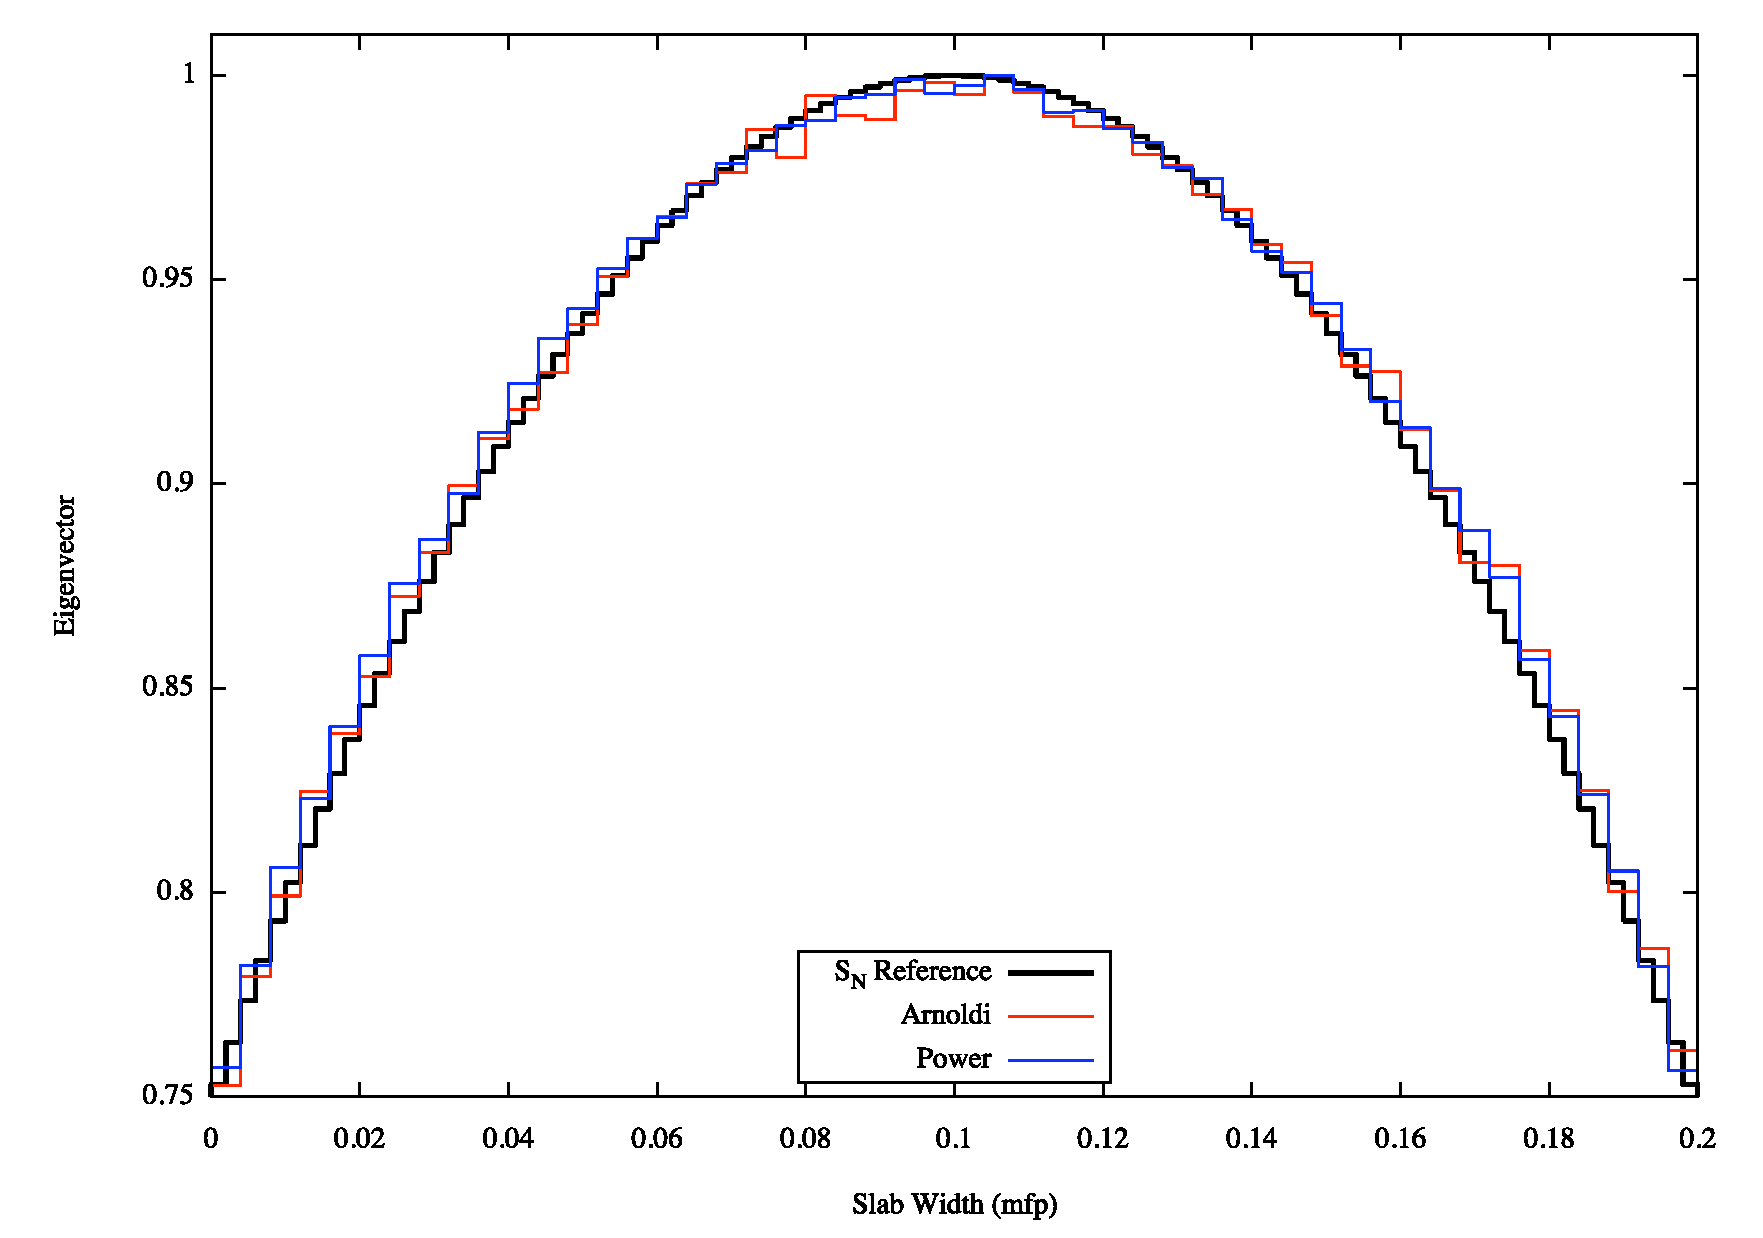
\includegraphics[width=\textwidth, keepaspectratio]{Arnoldi/Data/BasicFundamental-w02}
    % GNUPLOT: LaTeX picture with Postscript
\begingroup%
\makeatletter%
\newcommand{\GNUPLOTspecial}{%
  \@sanitize\catcode`\%=14\relax\special}%
\setlength{\unitlength}{0.0500bp}%
\begin{picture}(12960,8640)(0,0)%
  {\GNUPLOTspecial{"
%!PS-Adobe-2.0 EPSF-2.0
%%Title: BasicFundamental-w0.2.tex
%%Creator: gnuplot 4.3 patchlevel 0
%%CreationDate: Tue Jul 28 13:52:06 2009
%%DocumentFonts: 
%%BoundingBox: 0 0 648 432
%%EndComments
%%BeginProlog
/gnudict 256 dict def
gnudict begin
%
% The following true/false flags may be edited by hand if desired.
% The unit line width and grayscale image gamma correction may also be changed.
%
/Color true def
/Blacktext true def
/Solid true def
/Dashlength 1 def
/Landscape false def
/Level1 false def
/Rounded false def
/ClipToBoundingBox false def
/TransparentPatterns false def
/gnulinewidth 5.000 def
/userlinewidth gnulinewidth def
/Gamma 1.0 def
%
/vshift -66 def
/dl1 {
  10.0 Dashlength mul mul
  Rounded { currentlinewidth 0.75 mul sub dup 0 le { pop 0.01 } if } if
} def
/dl2 {
  10.0 Dashlength mul mul
  Rounded { currentlinewidth 0.75 mul add } if
} def
/hpt_ 31.5 def
/vpt_ 31.5 def
/hpt hpt_ def
/vpt vpt_ def
Level1 {} {
/SDict 10 dict def
systemdict /pdfmark known not {
  userdict /pdfmark systemdict /cleartomark get put
} if
SDict begin [
  /Title (BasicFundamental-w0.2.tex)
  /Subject (gnuplot plot)
  /Creator (gnuplot 4.3 patchlevel 0)
  /Author (Jeremy Conlin)
%  /Producer (gnuplot)
%  /Keywords ()
  /CreationDate (Tue Jul 28 13:52:06 2009)
  /DOCINFO pdfmark
end
} ifelse
/doclip {
  ClipToBoundingBox {
    newpath 0 0 moveto 648 0 lineto 648 432 lineto 0 432 lineto closepath
    clip
  } if
} def
%
% Gnuplot Prolog Version 4.2 (November 2007)
%
/M {moveto} bind def
/L {lineto} bind def
/R {rmoveto} bind def
/V {rlineto} bind def
/N {newpath moveto} bind def
/Z {closepath} bind def
/C {setrgbcolor} bind def
/f {rlineto fill} bind def
/Gshow {show} def   % May be redefined later in the file to support UTF-8
/vpt2 vpt 2 mul def
/hpt2 hpt 2 mul def
/Lshow {currentpoint stroke M 0 vshift R 
	Blacktext {gsave 0 setgray show grestore} {show} ifelse} def
/Rshow {currentpoint stroke M dup stringwidth pop neg vshift R
	Blacktext {gsave 0 setgray show grestore} {show} ifelse} def
/Cshow {currentpoint stroke M dup stringwidth pop -2 div vshift R 
	Blacktext {gsave 0 setgray show grestore} {show} ifelse} def
/UP {dup vpt_ mul /vpt exch def hpt_ mul /hpt exch def
  /hpt2 hpt 2 mul def /vpt2 vpt 2 mul def} def
/DL {Color {setrgbcolor Solid {pop []} if 0 setdash}
 {pop pop pop 0 setgray Solid {pop []} if 0 setdash} ifelse} def
/BL {stroke userlinewidth 2 mul setlinewidth
	Rounded {1 setlinejoin 1 setlinecap} if} def
/AL {stroke userlinewidth 2 div setlinewidth
	Rounded {1 setlinejoin 1 setlinecap} if} def
/UL {dup gnulinewidth mul /userlinewidth exch def
	dup 1 lt {pop 1} if 10 mul /udl exch def} def
/PL {stroke userlinewidth setlinewidth
	Rounded {1 setlinejoin 1 setlinecap} if} def
% Default Line colors
/LCw {1 1 1} def
/LCb {0 0 0} def
/LCa {0 0 0} def
/LC0 {1 0 0} def
/LC1 {0 1 0} def
/LC2 {0 0 1} def
/LC3 {1 0 1} def
/LC4 {0 1 1} def
/LC5 {1 1 0} def
/LC6 {0 0 0} def
/LC7 {1 0.3 0} def
/LC8 {0.5 0.5 0.5} def
% Default Line Types
/LTw {PL [] 1 setgray} def
/LTb {BL [] LCb DL} def
/LTa {AL [1 udl mul 2 udl mul] 0 setdash LCa setrgbcolor} def
/LT0 {PL [] LC0 DL} def
/LT1 {PL [4 dl1 2 dl2] LC1 DL} def
/LT2 {PL [2 dl1 3 dl2] LC2 DL} def
/LT3 {PL [1 dl1 1.5 dl2] LC3 DL} def
/LT4 {PL [6 dl1 2 dl2 1 dl1 2 dl2] LC4 DL} def
/LT5 {PL [3 dl1 3 dl2 1 dl1 3 dl2] LC5 DL} def
/LT6 {PL [2 dl1 2 dl2 2 dl1 6 dl2] LC6 DL} def
/LT7 {PL [1 dl1 2 dl2 6 dl1 2 dl2 1 dl1 2 dl2] LC7 DL} def
/LT8 {PL [2 dl1 2 dl2 2 dl1 2 dl2 2 dl1 2 dl2 2 dl1 4 dl2] LC8 DL} def
/Pnt {stroke [] 0 setdash gsave 1 setlinecap M 0 0 V stroke grestore} def
/Dia {stroke [] 0 setdash 2 copy vpt add M
  hpt neg vpt neg V hpt vpt neg V
  hpt vpt V hpt neg vpt V closepath stroke
  Pnt} def
/Pls {stroke [] 0 setdash vpt sub M 0 vpt2 V
  currentpoint stroke M
  hpt neg vpt neg R hpt2 0 V stroke
 } def
/Box {stroke [] 0 setdash 2 copy exch hpt sub exch vpt add M
  0 vpt2 neg V hpt2 0 V 0 vpt2 V
  hpt2 neg 0 V closepath stroke
  Pnt} def
/Crs {stroke [] 0 setdash exch hpt sub exch vpt add M
  hpt2 vpt2 neg V currentpoint stroke M
  hpt2 neg 0 R hpt2 vpt2 V stroke} def
/TriU {stroke [] 0 setdash 2 copy vpt 1.12 mul add M
  hpt neg vpt -1.62 mul V
  hpt 2 mul 0 V
  hpt neg vpt 1.62 mul V closepath stroke
  Pnt} def
/Star {2 copy Pls Crs} def
/BoxF {stroke [] 0 setdash exch hpt sub exch vpt add M
  0 vpt2 neg V hpt2 0 V 0 vpt2 V
  hpt2 neg 0 V closepath fill} def
/TriUF {stroke [] 0 setdash vpt 1.12 mul add M
  hpt neg vpt -1.62 mul V
  hpt 2 mul 0 V
  hpt neg vpt 1.62 mul V closepath fill} def
/TriD {stroke [] 0 setdash 2 copy vpt 1.12 mul sub M
  hpt neg vpt 1.62 mul V
  hpt 2 mul 0 V
  hpt neg vpt -1.62 mul V closepath stroke
  Pnt} def
/TriDF {stroke [] 0 setdash vpt 1.12 mul sub M
  hpt neg vpt 1.62 mul V
  hpt 2 mul 0 V
  hpt neg vpt -1.62 mul V closepath fill} def
/DiaF {stroke [] 0 setdash vpt add M
  hpt neg vpt neg V hpt vpt neg V
  hpt vpt V hpt neg vpt V closepath fill} def
/Pent {stroke [] 0 setdash 2 copy gsave
  translate 0 hpt M 4 {72 rotate 0 hpt L} repeat
  closepath stroke grestore Pnt} def
/PentF {stroke [] 0 setdash gsave
  translate 0 hpt M 4 {72 rotate 0 hpt L} repeat
  closepath fill grestore} def
/Circle {stroke [] 0 setdash 2 copy
  hpt 0 360 arc stroke Pnt} def
/CircleF {stroke [] 0 setdash hpt 0 360 arc fill} def
/C0 {BL [] 0 setdash 2 copy moveto vpt 90 450 arc} bind def
/C1 {BL [] 0 setdash 2 copy moveto
	2 copy vpt 0 90 arc closepath fill
	vpt 0 360 arc closepath} bind def
/C2 {BL [] 0 setdash 2 copy moveto
	2 copy vpt 90 180 arc closepath fill
	vpt 0 360 arc closepath} bind def
/C3 {BL [] 0 setdash 2 copy moveto
	2 copy vpt 0 180 arc closepath fill
	vpt 0 360 arc closepath} bind def
/C4 {BL [] 0 setdash 2 copy moveto
	2 copy vpt 180 270 arc closepath fill
	vpt 0 360 arc closepath} bind def
/C5 {BL [] 0 setdash 2 copy moveto
	2 copy vpt 0 90 arc
	2 copy moveto
	2 copy vpt 180 270 arc closepath fill
	vpt 0 360 arc} bind def
/C6 {BL [] 0 setdash 2 copy moveto
	2 copy vpt 90 270 arc closepath fill
	vpt 0 360 arc closepath} bind def
/C7 {BL [] 0 setdash 2 copy moveto
	2 copy vpt 0 270 arc closepath fill
	vpt 0 360 arc closepath} bind def
/C8 {BL [] 0 setdash 2 copy moveto
	2 copy vpt 270 360 arc closepath fill
	vpt 0 360 arc closepath} bind def
/C9 {BL [] 0 setdash 2 copy moveto
	2 copy vpt 270 450 arc closepath fill
	vpt 0 360 arc closepath} bind def
/C10 {BL [] 0 setdash 2 copy 2 copy moveto vpt 270 360 arc closepath fill
	2 copy moveto
	2 copy vpt 90 180 arc closepath fill
	vpt 0 360 arc closepath} bind def
/C11 {BL [] 0 setdash 2 copy moveto
	2 copy vpt 0 180 arc closepath fill
	2 copy moveto
	2 copy vpt 270 360 arc closepath fill
	vpt 0 360 arc closepath} bind def
/C12 {BL [] 0 setdash 2 copy moveto
	2 copy vpt 180 360 arc closepath fill
	vpt 0 360 arc closepath} bind def
/C13 {BL [] 0 setdash 2 copy moveto
	2 copy vpt 0 90 arc closepath fill
	2 copy moveto
	2 copy vpt 180 360 arc closepath fill
	vpt 0 360 arc closepath} bind def
/C14 {BL [] 0 setdash 2 copy moveto
	2 copy vpt 90 360 arc closepath fill
	vpt 0 360 arc} bind def
/C15 {BL [] 0 setdash 2 copy vpt 0 360 arc closepath fill
	vpt 0 360 arc closepath} bind def
/Rec {newpath 4 2 roll moveto 1 index 0 rlineto 0 exch rlineto
	neg 0 rlineto closepath} bind def
/Square {dup Rec} bind def
/Bsquare {vpt sub exch vpt sub exch vpt2 Square} bind def
/S0 {BL [] 0 setdash 2 copy moveto 0 vpt rlineto BL Bsquare} bind def
/S1 {BL [] 0 setdash 2 copy vpt Square fill Bsquare} bind def
/S2 {BL [] 0 setdash 2 copy exch vpt sub exch vpt Square fill Bsquare} bind def
/S3 {BL [] 0 setdash 2 copy exch vpt sub exch vpt2 vpt Rec fill Bsquare} bind def
/S4 {BL [] 0 setdash 2 copy exch vpt sub exch vpt sub vpt Square fill Bsquare} bind def
/S5 {BL [] 0 setdash 2 copy 2 copy vpt Square fill
	exch vpt sub exch vpt sub vpt Square fill Bsquare} bind def
/S6 {BL [] 0 setdash 2 copy exch vpt sub exch vpt sub vpt vpt2 Rec fill Bsquare} bind def
/S7 {BL [] 0 setdash 2 copy exch vpt sub exch vpt sub vpt vpt2 Rec fill
	2 copy vpt Square fill Bsquare} bind def
/S8 {BL [] 0 setdash 2 copy vpt sub vpt Square fill Bsquare} bind def
/S9 {BL [] 0 setdash 2 copy vpt sub vpt vpt2 Rec fill Bsquare} bind def
/S10 {BL [] 0 setdash 2 copy vpt sub vpt Square fill 2 copy exch vpt sub exch vpt Square fill
	Bsquare} bind def
/S11 {BL [] 0 setdash 2 copy vpt sub vpt Square fill 2 copy exch vpt sub exch vpt2 vpt Rec fill
	Bsquare} bind def
/S12 {BL [] 0 setdash 2 copy exch vpt sub exch vpt sub vpt2 vpt Rec fill Bsquare} bind def
/S13 {BL [] 0 setdash 2 copy exch vpt sub exch vpt sub vpt2 vpt Rec fill
	2 copy vpt Square fill Bsquare} bind def
/S14 {BL [] 0 setdash 2 copy exch vpt sub exch vpt sub vpt2 vpt Rec fill
	2 copy exch vpt sub exch vpt Square fill Bsquare} bind def
/S15 {BL [] 0 setdash 2 copy Bsquare fill Bsquare} bind def
/D0 {gsave translate 45 rotate 0 0 S0 stroke grestore} bind def
/D1 {gsave translate 45 rotate 0 0 S1 stroke grestore} bind def
/D2 {gsave translate 45 rotate 0 0 S2 stroke grestore} bind def
/D3 {gsave translate 45 rotate 0 0 S3 stroke grestore} bind def
/D4 {gsave translate 45 rotate 0 0 S4 stroke grestore} bind def
/D5 {gsave translate 45 rotate 0 0 S5 stroke grestore} bind def
/D6 {gsave translate 45 rotate 0 0 S6 stroke grestore} bind def
/D7 {gsave translate 45 rotate 0 0 S7 stroke grestore} bind def
/D8 {gsave translate 45 rotate 0 0 S8 stroke grestore} bind def
/D9 {gsave translate 45 rotate 0 0 S9 stroke grestore} bind def
/D10 {gsave translate 45 rotate 0 0 S10 stroke grestore} bind def
/D11 {gsave translate 45 rotate 0 0 S11 stroke grestore} bind def
/D12 {gsave translate 45 rotate 0 0 S12 stroke grestore} bind def
/D13 {gsave translate 45 rotate 0 0 S13 stroke grestore} bind def
/D14 {gsave translate 45 rotate 0 0 S14 stroke grestore} bind def
/D15 {gsave translate 45 rotate 0 0 S15 stroke grestore} bind def
/DiaE {stroke [] 0 setdash vpt add M
  hpt neg vpt neg V hpt vpt neg V
  hpt vpt V hpt neg vpt V closepath stroke} def
/BoxE {stroke [] 0 setdash exch hpt sub exch vpt add M
  0 vpt2 neg V hpt2 0 V 0 vpt2 V
  hpt2 neg 0 V closepath stroke} def
/TriUE {stroke [] 0 setdash vpt 1.12 mul add M
  hpt neg vpt -1.62 mul V
  hpt 2 mul 0 V
  hpt neg vpt 1.62 mul V closepath stroke} def
/TriDE {stroke [] 0 setdash vpt 1.12 mul sub M
  hpt neg vpt 1.62 mul V
  hpt 2 mul 0 V
  hpt neg vpt -1.62 mul V closepath stroke} def
/PentE {stroke [] 0 setdash gsave
  translate 0 hpt M 4 {72 rotate 0 hpt L} repeat
  closepath stroke grestore} def
/CircE {stroke [] 0 setdash 
  hpt 0 360 arc stroke} def
/Opaque {gsave closepath 1 setgray fill grestore 0 setgray closepath} def
/DiaW {stroke [] 0 setdash vpt add M
  hpt neg vpt neg V hpt vpt neg V
  hpt vpt V hpt neg vpt V Opaque stroke} def
/BoxW {stroke [] 0 setdash exch hpt sub exch vpt add M
  0 vpt2 neg V hpt2 0 V 0 vpt2 V
  hpt2 neg 0 V Opaque stroke} def
/TriUW {stroke [] 0 setdash vpt 1.12 mul add M
  hpt neg vpt -1.62 mul V
  hpt 2 mul 0 V
  hpt neg vpt 1.62 mul V Opaque stroke} def
/TriDW {stroke [] 0 setdash vpt 1.12 mul sub M
  hpt neg vpt 1.62 mul V
  hpt 2 mul 0 V
  hpt neg vpt -1.62 mul V Opaque stroke} def
/PentW {stroke [] 0 setdash gsave
  translate 0 hpt M 4 {72 rotate 0 hpt L} repeat
  Opaque stroke grestore} def
/CircW {stroke [] 0 setdash 
  hpt 0 360 arc Opaque stroke} def
/BoxFill {gsave Rec 1 setgray fill grestore} def
/Density {
  /Fillden exch def
  currentrgbcolor
  /ColB exch def /ColG exch def /ColR exch def
  /ColR ColR Fillden mul Fillden sub 1 add def
  /ColG ColG Fillden mul Fillden sub 1 add def
  /ColB ColB Fillden mul Fillden sub 1 add def
  ColR ColG ColB setrgbcolor} def
/BoxColFill {gsave Rec PolyFill} def
/PolyFill {gsave Density fill grestore grestore} def
/h {rlineto rlineto rlineto gsave closepath fill grestore} bind def
%
% PostScript Level 1 Pattern Fill routine for rectangles
% Usage: x y w h s a XX PatternFill
%	x,y = lower left corner of box to be filled
%	w,h = width and height of box
%	  a = angle in degrees between lines and x-axis
%	 XX = 0/1 for no/yes cross-hatch
%
/PatternFill {gsave /PFa [ 9 2 roll ] def
  PFa 0 get PFa 2 get 2 div add PFa 1 get PFa 3 get 2 div add translate
  PFa 2 get -2 div PFa 3 get -2 div PFa 2 get PFa 3 get Rec
  gsave 1 setgray fill grestore clip
  currentlinewidth 0.5 mul setlinewidth
  /PFs PFa 2 get dup mul PFa 3 get dup mul add sqrt def
  0 0 M PFa 5 get rotate PFs -2 div dup translate
  0 1 PFs PFa 4 get div 1 add floor cvi
	{PFa 4 get mul 0 M 0 PFs V} for
  0 PFa 6 get ne {
	0 1 PFs PFa 4 get div 1 add floor cvi
	{PFa 4 get mul 0 2 1 roll M PFs 0 V} for
 } if
  stroke grestore} def
%
/languagelevel where
 {pop languagelevel} {1} ifelse
 2 lt
	{/InterpretLevel1 true def}
	{/InterpretLevel1 Level1 def}
 ifelse
%
% PostScript level 2 pattern fill definitions
%
/Level2PatternFill {
/Tile8x8 {/PaintType 2 /PatternType 1 /TilingType 1 /BBox [0 0 8 8] /XStep 8 /YStep 8}
	bind def
/KeepColor {currentrgbcolor [/Pattern /DeviceRGB] setcolorspace} bind def
<< Tile8x8
 /PaintProc {0.5 setlinewidth pop 0 0 M 8 8 L 0 8 M 8 0 L stroke} 
>> matrix makepattern
/Pat1 exch def
<< Tile8x8
 /PaintProc {0.5 setlinewidth pop 0 0 M 8 8 L 0 8 M 8 0 L stroke
	0 4 M 4 8 L 8 4 L 4 0 L 0 4 L stroke}
>> matrix makepattern
/Pat2 exch def
<< Tile8x8
 /PaintProc {0.5 setlinewidth pop 0 0 M 0 8 L
	8 8 L 8 0 L 0 0 L fill}
>> matrix makepattern
/Pat3 exch def
<< Tile8x8
 /PaintProc {0.5 setlinewidth pop -4 8 M 8 -4 L
	0 12 M 12 0 L stroke}
>> matrix makepattern
/Pat4 exch def
<< Tile8x8
 /PaintProc {0.5 setlinewidth pop -4 0 M 8 12 L
	0 -4 M 12 8 L stroke}
>> matrix makepattern
/Pat5 exch def
<< Tile8x8
 /PaintProc {0.5 setlinewidth pop -2 8 M 4 -4 L
	0 12 M 8 -4 L 4 12 M 10 0 L stroke}
>> matrix makepattern
/Pat6 exch def
<< Tile8x8
 /PaintProc {0.5 setlinewidth pop -2 0 M 4 12 L
	0 -4 M 8 12 L 4 -4 M 10 8 L stroke}
>> matrix makepattern
/Pat7 exch def
<< Tile8x8
 /PaintProc {0.5 setlinewidth pop 8 -2 M -4 4 L
	12 0 M -4 8 L 12 4 M 0 10 L stroke}
>> matrix makepattern
/Pat8 exch def
<< Tile8x8
 /PaintProc {0.5 setlinewidth pop 0 -2 M 12 4 L
	-4 0 M 12 8 L -4 4 M 8 10 L stroke}
>> matrix makepattern
/Pat9 exch def
/Pattern1 {PatternBgnd KeepColor Pat1 setpattern} bind def
/Pattern2 {PatternBgnd KeepColor Pat2 setpattern} bind def
/Pattern3 {PatternBgnd KeepColor Pat3 setpattern} bind def
/Pattern4 {PatternBgnd KeepColor Landscape {Pat5} {Pat4} ifelse setpattern} bind def
/Pattern5 {PatternBgnd KeepColor Landscape {Pat4} {Pat5} ifelse setpattern} bind def
/Pattern6 {PatternBgnd KeepColor Landscape {Pat9} {Pat6} ifelse setpattern} bind def
/Pattern7 {PatternBgnd KeepColor Landscape {Pat8} {Pat7} ifelse setpattern} bind def
} def
%
%
%End of PostScript Level 2 code
%
/PatternBgnd {
  TransparentPatterns {} {gsave 1 setgray fill grestore} ifelse
} def
%
% Substitute for Level 2 pattern fill codes with
% grayscale if Level 2 support is not selected.
%
/Level1PatternFill {
/Pattern1 {0.250 Density} bind def
/Pattern2 {0.500 Density} bind def
/Pattern3 {0.750 Density} bind def
/Pattern4 {0.125 Density} bind def
/Pattern5 {0.375 Density} bind def
/Pattern6 {0.625 Density} bind def
/Pattern7 {0.875 Density} bind def
} def
%
% Now test for support of Level 2 code
%
Level1 {Level1PatternFill} {Level2PatternFill} ifelse
%
/Symbol-Oblique /Symbol findfont [1 0 .167 1 0 0] makefont
dup length dict begin {1 index /FID eq {pop pop} {def} ifelse} forall
currentdict end definefont pop
end
%%EndProlog
gnudict begin
gsave
doclip
0 0 translate
0.050 0.050 scale
0 setgray
newpath
1.000 UL
LTb
1220 640 M
63 0 V
11276 0 R
-63 0 V
1220 2132 M
63 0 V
11276 0 R
-63 0 V
1220 3624 M
63 0 V
11276 0 R
-63 0 V
1220 5116 M
63 0 V
11276 0 R
-63 0 V
1220 6608 M
63 0 V
11276 0 R
-63 0 V
1220 8101 M
63 0 V
11276 0 R
-63 0 V
1220 640 M
0 63 V
0 7696 R
0 -63 V
2354 640 M
0 63 V
0 7696 R
0 -63 V
3488 640 M
0 63 V
0 7696 R
0 -63 V
4622 640 M
0 63 V
0 7696 R
0 -63 V
5756 640 M
0 63 V
0 7696 R
0 -63 V
6890 640 M
0 63 V
0 7696 R
0 -63 V
8023 640 M
0 63 V
0 7696 R
0 -63 V
9157 640 M
0 63 V
0 7696 R
0 -63 V
10291 640 M
0 63 V
0 7696 R
0 -63 V
11425 640 M
0 63 V
0 7696 R
0 -63 V
12559 640 M
0 63 V
0 7696 R
0 -63 V
stroke
1220 8399 N
0 -7759 V
11339 0 V
0 7759 V
-11339 0 V
Z stroke
LCb setrgbcolor
LTb
LCb setrgbcolor
LTb
LCb setrgbcolor
LTb
LCb setrgbcolor
LTb
1.000 UP
1.000 UL
LTb
1.000 UL
LTb
5718 703 N
0 800 V
2342 0 V
0 -800 V
-2342 0 V
Z stroke
5718 1503 M
2342 0 V
stroke
2.000 UL
LTb
LCb setrgbcolor
LTb
7398 1303 M
543 0 V
1220 640 M
0 90 V
113 0 V
0 310 V
114 0 V
0 302 V
113 0 V
0 296 V
114 0 V
0 287 V
113 0 V
0 280 V
113 0 V
0 272 V
114 0 V
0 266 V
113 0 V
0 258 V
114 0 V
0 251 V
113 0 V
0 244 V
113 0 V
0 238 V
114 0 V
0 230 V
113 0 V
0 224 V
113 0 V
0 217 V
114 0 V
0 209 V
113 0 V
0 205 V
114 0 V
0 196 V
113 0 V
0 191 V
113 0 V
0 185 V
114 0 V
0 177 V
113 0 V
0 172 V
114 0 V
0 165 V
113 0 V
0 159 V
113 0 V
0 153 V
114 0 V
0 146 V
113 0 V
0 141 V
114 0 V
0 134 V
113 0 V
0 129 V
113 0 V
0 121 V
114 0 V
0 117 V
113 0 V
0 111 V
113 0 V
0 104 V
114 0 V
0 98 V
113 0 V
0 93 V
114 0 V
0 87 V
113 0 V
0 80 V
113 0 V
0 76 V
114 0 V
0 69 V
113 0 V
0 62 V
114 0 V
0 58 V
113 0 V
0 52 V
113 0 V
0 46 V
114 0 V
0 39 V
113 0 V
0 35 V
114 0 V
0 29 V
113 0 V
0 23 V
113 0 V
0 17 V
114 0 V
0 11 V
113 0 V
0 6 V
170 0 V
0 -6 V
170 0 V
stroke 7116 8095 M
0 -11 V
114 0 V
0 -17 V
113 0 V
0 -23 V
113 0 V
0 -29 V
114 0 V
0 -35 V
113 0 V
0 -39 V
114 0 V
0 -46 V
113 0 V
0 -52 V
113 0 V
0 -58 V
114 0 V
0 -62 V
113 0 V
0 -69 V
114 0 V
0 -76 V
113 0 V
0 -80 V
113 0 V
0 -87 V
114 0 V
0 -93 V
113 0 V
0 -98 V
114 0 V
0 -104 V
113 0 V
0 -111 V
113 0 V
0 -117 V
114 0 V
0 -121 V
113 0 V
0 -129 V
113 0 V
0 -134 V
114 0 V
0 -141 V
113 0 V
0 -146 V
114 0 V
0 -153 V
113 0 V
0 -159 V
113 0 V
0 -165 V
114 0 V
0 -172 V
113 0 V
0 -177 V
114 0 V
0 -185 V
113 0 V
0 -191 V
113 0 V
0 -196 V
114 0 V
0 -205 V
113 0 V
0 -209 V
114 0 V
0 -217 V
113 0 V
0 -224 V
113 0 V
0 -230 V
114 0 V
0 -238 V
113 0 V
0 -244 V
113 0 V
0 -251 V
114 0 V
0 -258 V
113 0 V
0 -266 V
114 0 V
0 -272 V
113 0 V
0 -280 V
113 0 V
0 -287 V
114 0 V
0 -296 V
113 0 V
0 -302 V
114 0 V
0 -310 V
113 0 V
0 -90 V
stroke
1.000 UL
LT0
LCb setrgbcolor
LT0
7398 1103 M
543 0 V
1220 640 M
0 279 V
227 0 V
0 753 V
227 0 V
0 620 V
226 0 V
0 544 V
227 0 V
0 637 V
227 0 V
0 460 V
227 0 V
0 391 V
226 0 V
0 547 V
227 0 V
0 324 V
227 0 V
0 346 V
227 0 V
0 323 V
227 0 V
0 228 V
226 0 V
0 387 V
227 0 V
0 247 V
227 0 V
0 216 V
227 0 V
0 208 V
226 0 V
0 223 V
227 0 V
0 88 V
227 0 V
0 153 V
227 0 V
0 196 V
227 0 V
0 71 V
226 0 V
0 76 V
227 0 V
0 50 V
227 0 V
0 4 V
227 0 V
0 -19 V
226 0 V
0 109 V
227 0 V
0 -97 V
227 0 V
0 15 V
227 0 V
0 -33 V
227 0 V
0 -106 V
226 0 V
0 -85 V
227 0 V
0 -175 V
227 0 V
0 -74 V
227 0 V
0 -175 V
227 0 V
0 -186 V
226 0 V
0 -254 V
227 0 V
0 -268 V
227 0 V
0 -177 V
227 0 V
0 -284 V
226 0 V
0 -341 V
227 0 V
0 -341 V
227 0 V
0 -349 V
227 0 V
0 -394 V
227 0 V
0 -393 V
226 0 V
0 -411 V
227 0 V
0 -505 V
227 0 V
0 -586 V
227 0 V
0 -654 V
226 0 V
0 -550 V
227 0 V
0 -820 V
227 0 V
0 -218 V
stroke
LT2
LCb setrgbcolor
LT2
7398 903 M
543 0 V
1220 640 M
0 7461 V
227 0 V
0 298 V
10885 0 R
0 -161 V
227 0 V
0 -7598 V
stroke
LTb
1220 8399 N
0 -7759 V
11339 0 V
0 7759 V
-11339 0 V
Z stroke
1.000 UP
1.000 UL
LTb
stroke
grestore
end
showpage
  }}%
  \put(7278,903){\makebox(0,0)[r]{\strut{}Arnoldi}}%
  \put(7278,1103){\makebox(0,0)[r]{\strut{}Power}}%
  \put(7278,1303){\makebox(0,0)[r]{\strut{}$S_N$ Reference}}%
  \put(6889,140){\makebox(0,0){\strut{}Slab Width (mfp)}}%
  \put(280,4519){%
  \special{ps: gsave currentpoint currentpoint translate
270 rotate neg exch neg exch translate}%
  \makebox(0,0){\strut{}Eigenvector}%
  \special{ps: currentpoint grestore moveto}%
  }%
  \put(12559,440){\makebox(0,0){\strut{} 0.2}}%
  \put(11425,440){\makebox(0,0){\strut{} 0.18}}%
  \put(10291,440){\makebox(0,0){\strut{} 0.16}}%
  \put(9157,440){\makebox(0,0){\strut{} 0.14}}%
  \put(8023,440){\makebox(0,0){\strut{} 0.12}}%
  \put(6890,440){\makebox(0,0){\strut{} 0.1}}%
  \put(5756,440){\makebox(0,0){\strut{} 0.08}}%
  \put(4622,440){\makebox(0,0){\strut{} 0.06}}%
  \put(3488,440){\makebox(0,0){\strut{} 0.04}}%
  \put(2354,440){\makebox(0,0){\strut{} 0.02}}%
  \put(1220,440){\makebox(0,0){\strut{} 0}}%
  \put(1100,8101){\makebox(0,0)[r]{\strut{} 1}}%
  \put(1100,6608){\makebox(0,0)[r]{\strut{} 0.95}}%
  \put(1100,5116){\makebox(0,0)[r]{\strut{} 0.9}}%
  \put(1100,3624){\makebox(0,0)[r]{\strut{} 0.85}}%
  \put(1100,2132){\makebox(0,0)[r]{\strut{} 0.8}}%
  \put(1100,640){\makebox(0,0)[r]{\strut{} 0.75}}%
\end{picture}%
\endgroup
\endinput

    \caption{Fundamental eigenvector estimates from the power method and Arnoldi's method for the 0.2 mfp wide slab.  The heavy line shows the S$_\mathrm{N}$ solution.}
    \label{fig:BasicFundamentalW02}
\end{sidewaysfigure}
\end{comment}

\begin{figure}\centering
    \subfloat[Eigenvalue estimates]{\label{fig:BasicValuesW2}% GNUPLOT: LaTeX picture with Postscript
\begingroup%
\makeatletter%
\newcommand{\GNUPLOTspecial}{%
  \@sanitize\catcode`\%=14\relax\special}%
\setlength{\unitlength}{0.0500bp}%
\begin{picture}(8640,5760)(0,0)%
  {\GNUPLOTspecial{"
%!PS-Adobe-2.0 EPSF-2.0
%%Title: BasicValues-w2.tex
%%Creator: gnuplot 4.3 patchlevel 0
%%CreationDate: Tue Jul 28 13:52:07 2009
%%DocumentFonts: 
%%BoundingBox: 0 0 432 288
%%EndComments
%%BeginProlog
/gnudict 256 dict def
gnudict begin
%
% The following true/false flags may be edited by hand if desired.
% The unit line width and grayscale image gamma correction may also be changed.
%
/Color true def
/Blacktext true def
/Solid true def
/Dashlength 1 def
/Landscape false def
/Level1 false def
/Rounded false def
/ClipToBoundingBox false def
/TransparentPatterns false def
/gnulinewidth 5.000 def
/userlinewidth gnulinewidth def
/Gamma 1.0 def
%
/vshift -66 def
/dl1 {
  10.0 Dashlength mul mul
  Rounded { currentlinewidth 0.75 mul sub dup 0 le { pop 0.01 } if } if
} def
/dl2 {
  10.0 Dashlength mul mul
  Rounded { currentlinewidth 0.75 mul add } if
} def
/hpt_ 31.5 def
/vpt_ 31.5 def
/hpt hpt_ def
/vpt vpt_ def
Level1 {} {
/SDict 10 dict def
systemdict /pdfmark known not {
  userdict /pdfmark systemdict /cleartomark get put
} if
SDict begin [
  /Title (BasicValues-w2.tex)
  /Subject (gnuplot plot)
  /Creator (gnuplot 4.3 patchlevel 0)
  /Author (Jeremy Conlin)
%  /Producer (gnuplot)
%  /Keywords ()
  /CreationDate (Tue Jul 28 13:52:07 2009)
  /DOCINFO pdfmark
end
} ifelse
/doclip {
  ClipToBoundingBox {
    newpath 0 0 moveto 432 0 lineto 432 288 lineto 0 288 lineto closepath
    clip
  } if
} def
%
% Gnuplot Prolog Version 4.2 (November 2007)
%
/M {moveto} bind def
/L {lineto} bind def
/R {rmoveto} bind def
/V {rlineto} bind def
/N {newpath moveto} bind def
/Z {closepath} bind def
/C {setrgbcolor} bind def
/f {rlineto fill} bind def
/Gshow {show} def   % May be redefined later in the file to support UTF-8
/vpt2 vpt 2 mul def
/hpt2 hpt 2 mul def
/Lshow {currentpoint stroke M 0 vshift R 
	Blacktext {gsave 0 setgray show grestore} {show} ifelse} def
/Rshow {currentpoint stroke M dup stringwidth pop neg vshift R
	Blacktext {gsave 0 setgray show grestore} {show} ifelse} def
/Cshow {currentpoint stroke M dup stringwidth pop -2 div vshift R 
	Blacktext {gsave 0 setgray show grestore} {show} ifelse} def
/UP {dup vpt_ mul /vpt exch def hpt_ mul /hpt exch def
  /hpt2 hpt 2 mul def /vpt2 vpt 2 mul def} def
/DL {Color {setrgbcolor Solid {pop []} if 0 setdash}
 {pop pop pop 0 setgray Solid {pop []} if 0 setdash} ifelse} def
/BL {stroke userlinewidth 2 mul setlinewidth
	Rounded {1 setlinejoin 1 setlinecap} if} def
/AL {stroke userlinewidth 2 div setlinewidth
	Rounded {1 setlinejoin 1 setlinecap} if} def
/UL {dup gnulinewidth mul /userlinewidth exch def
	dup 1 lt {pop 1} if 10 mul /udl exch def} def
/PL {stroke userlinewidth setlinewidth
	Rounded {1 setlinejoin 1 setlinecap} if} def
% Default Line colors
/LCw {1 1 1} def
/LCb {0 0 0} def
/LCa {0 0 0} def
/LC0 {1 0 0} def
/LC1 {0 1 0} def
/LC2 {0 0 1} def
/LC3 {1 0 1} def
/LC4 {0 1 1} def
/LC5 {1 1 0} def
/LC6 {0 0 0} def
/LC7 {1 0.3 0} def
/LC8 {0.5 0.5 0.5} def
% Default Line Types
/LTw {PL [] 1 setgray} def
/LTb {BL [] LCb DL} def
/LTa {AL [1 udl mul 2 udl mul] 0 setdash LCa setrgbcolor} def
/LT0 {PL [] LC0 DL} def
/LT1 {PL [4 dl1 2 dl2] LC1 DL} def
/LT2 {PL [2 dl1 3 dl2] LC2 DL} def
/LT3 {PL [1 dl1 1.5 dl2] LC3 DL} def
/LT4 {PL [6 dl1 2 dl2 1 dl1 2 dl2] LC4 DL} def
/LT5 {PL [3 dl1 3 dl2 1 dl1 3 dl2] LC5 DL} def
/LT6 {PL [2 dl1 2 dl2 2 dl1 6 dl2] LC6 DL} def
/LT7 {PL [1 dl1 2 dl2 6 dl1 2 dl2 1 dl1 2 dl2] LC7 DL} def
/LT8 {PL [2 dl1 2 dl2 2 dl1 2 dl2 2 dl1 2 dl2 2 dl1 4 dl2] LC8 DL} def
/Pnt {stroke [] 0 setdash gsave 1 setlinecap M 0 0 V stroke grestore} def
/Dia {stroke [] 0 setdash 2 copy vpt add M
  hpt neg vpt neg V hpt vpt neg V
  hpt vpt V hpt neg vpt V closepath stroke
  Pnt} def
/Pls {stroke [] 0 setdash vpt sub M 0 vpt2 V
  currentpoint stroke M
  hpt neg vpt neg R hpt2 0 V stroke
 } def
/Box {stroke [] 0 setdash 2 copy exch hpt sub exch vpt add M
  0 vpt2 neg V hpt2 0 V 0 vpt2 V
  hpt2 neg 0 V closepath stroke
  Pnt} def
/Crs {stroke [] 0 setdash exch hpt sub exch vpt add M
  hpt2 vpt2 neg V currentpoint stroke M
  hpt2 neg 0 R hpt2 vpt2 V stroke} def
/TriU {stroke [] 0 setdash 2 copy vpt 1.12 mul add M
  hpt neg vpt -1.62 mul V
  hpt 2 mul 0 V
  hpt neg vpt 1.62 mul V closepath stroke
  Pnt} def
/Star {2 copy Pls Crs} def
/BoxF {stroke [] 0 setdash exch hpt sub exch vpt add M
  0 vpt2 neg V hpt2 0 V 0 vpt2 V
  hpt2 neg 0 V closepath fill} def
/TriUF {stroke [] 0 setdash vpt 1.12 mul add M
  hpt neg vpt -1.62 mul V
  hpt 2 mul 0 V
  hpt neg vpt 1.62 mul V closepath fill} def
/TriD {stroke [] 0 setdash 2 copy vpt 1.12 mul sub M
  hpt neg vpt 1.62 mul V
  hpt 2 mul 0 V
  hpt neg vpt -1.62 mul V closepath stroke
  Pnt} def
/TriDF {stroke [] 0 setdash vpt 1.12 mul sub M
  hpt neg vpt 1.62 mul V
  hpt 2 mul 0 V
  hpt neg vpt -1.62 mul V closepath fill} def
/DiaF {stroke [] 0 setdash vpt add M
  hpt neg vpt neg V hpt vpt neg V
  hpt vpt V hpt neg vpt V closepath fill} def
/Pent {stroke [] 0 setdash 2 copy gsave
  translate 0 hpt M 4 {72 rotate 0 hpt L} repeat
  closepath stroke grestore Pnt} def
/PentF {stroke [] 0 setdash gsave
  translate 0 hpt M 4 {72 rotate 0 hpt L} repeat
  closepath fill grestore} def
/Circle {stroke [] 0 setdash 2 copy
  hpt 0 360 arc stroke Pnt} def
/CircleF {stroke [] 0 setdash hpt 0 360 arc fill} def
/C0 {BL [] 0 setdash 2 copy moveto vpt 90 450 arc} bind def
/C1 {BL [] 0 setdash 2 copy moveto
	2 copy vpt 0 90 arc closepath fill
	vpt 0 360 arc closepath} bind def
/C2 {BL [] 0 setdash 2 copy moveto
	2 copy vpt 90 180 arc closepath fill
	vpt 0 360 arc closepath} bind def
/C3 {BL [] 0 setdash 2 copy moveto
	2 copy vpt 0 180 arc closepath fill
	vpt 0 360 arc closepath} bind def
/C4 {BL [] 0 setdash 2 copy moveto
	2 copy vpt 180 270 arc closepath fill
	vpt 0 360 arc closepath} bind def
/C5 {BL [] 0 setdash 2 copy moveto
	2 copy vpt 0 90 arc
	2 copy moveto
	2 copy vpt 180 270 arc closepath fill
	vpt 0 360 arc} bind def
/C6 {BL [] 0 setdash 2 copy moveto
	2 copy vpt 90 270 arc closepath fill
	vpt 0 360 arc closepath} bind def
/C7 {BL [] 0 setdash 2 copy moveto
	2 copy vpt 0 270 arc closepath fill
	vpt 0 360 arc closepath} bind def
/C8 {BL [] 0 setdash 2 copy moveto
	2 copy vpt 270 360 arc closepath fill
	vpt 0 360 arc closepath} bind def
/C9 {BL [] 0 setdash 2 copy moveto
	2 copy vpt 270 450 arc closepath fill
	vpt 0 360 arc closepath} bind def
/C10 {BL [] 0 setdash 2 copy 2 copy moveto vpt 270 360 arc closepath fill
	2 copy moveto
	2 copy vpt 90 180 arc closepath fill
	vpt 0 360 arc closepath} bind def
/C11 {BL [] 0 setdash 2 copy moveto
	2 copy vpt 0 180 arc closepath fill
	2 copy moveto
	2 copy vpt 270 360 arc closepath fill
	vpt 0 360 arc closepath} bind def
/C12 {BL [] 0 setdash 2 copy moveto
	2 copy vpt 180 360 arc closepath fill
	vpt 0 360 arc closepath} bind def
/C13 {BL [] 0 setdash 2 copy moveto
	2 copy vpt 0 90 arc closepath fill
	2 copy moveto
	2 copy vpt 180 360 arc closepath fill
	vpt 0 360 arc closepath} bind def
/C14 {BL [] 0 setdash 2 copy moveto
	2 copy vpt 90 360 arc closepath fill
	vpt 0 360 arc} bind def
/C15 {BL [] 0 setdash 2 copy vpt 0 360 arc closepath fill
	vpt 0 360 arc closepath} bind def
/Rec {newpath 4 2 roll moveto 1 index 0 rlineto 0 exch rlineto
	neg 0 rlineto closepath} bind def
/Square {dup Rec} bind def
/Bsquare {vpt sub exch vpt sub exch vpt2 Square} bind def
/S0 {BL [] 0 setdash 2 copy moveto 0 vpt rlineto BL Bsquare} bind def
/S1 {BL [] 0 setdash 2 copy vpt Square fill Bsquare} bind def
/S2 {BL [] 0 setdash 2 copy exch vpt sub exch vpt Square fill Bsquare} bind def
/S3 {BL [] 0 setdash 2 copy exch vpt sub exch vpt2 vpt Rec fill Bsquare} bind def
/S4 {BL [] 0 setdash 2 copy exch vpt sub exch vpt sub vpt Square fill Bsquare} bind def
/S5 {BL [] 0 setdash 2 copy 2 copy vpt Square fill
	exch vpt sub exch vpt sub vpt Square fill Bsquare} bind def
/S6 {BL [] 0 setdash 2 copy exch vpt sub exch vpt sub vpt vpt2 Rec fill Bsquare} bind def
/S7 {BL [] 0 setdash 2 copy exch vpt sub exch vpt sub vpt vpt2 Rec fill
	2 copy vpt Square fill Bsquare} bind def
/S8 {BL [] 0 setdash 2 copy vpt sub vpt Square fill Bsquare} bind def
/S9 {BL [] 0 setdash 2 copy vpt sub vpt vpt2 Rec fill Bsquare} bind def
/S10 {BL [] 0 setdash 2 copy vpt sub vpt Square fill 2 copy exch vpt sub exch vpt Square fill
	Bsquare} bind def
/S11 {BL [] 0 setdash 2 copy vpt sub vpt Square fill 2 copy exch vpt sub exch vpt2 vpt Rec fill
	Bsquare} bind def
/S12 {BL [] 0 setdash 2 copy exch vpt sub exch vpt sub vpt2 vpt Rec fill Bsquare} bind def
/S13 {BL [] 0 setdash 2 copy exch vpt sub exch vpt sub vpt2 vpt Rec fill
	2 copy vpt Square fill Bsquare} bind def
/S14 {BL [] 0 setdash 2 copy exch vpt sub exch vpt sub vpt2 vpt Rec fill
	2 copy exch vpt sub exch vpt Square fill Bsquare} bind def
/S15 {BL [] 0 setdash 2 copy Bsquare fill Bsquare} bind def
/D0 {gsave translate 45 rotate 0 0 S0 stroke grestore} bind def
/D1 {gsave translate 45 rotate 0 0 S1 stroke grestore} bind def
/D2 {gsave translate 45 rotate 0 0 S2 stroke grestore} bind def
/D3 {gsave translate 45 rotate 0 0 S3 stroke grestore} bind def
/D4 {gsave translate 45 rotate 0 0 S4 stroke grestore} bind def
/D5 {gsave translate 45 rotate 0 0 S5 stroke grestore} bind def
/D6 {gsave translate 45 rotate 0 0 S6 stroke grestore} bind def
/D7 {gsave translate 45 rotate 0 0 S7 stroke grestore} bind def
/D8 {gsave translate 45 rotate 0 0 S8 stroke grestore} bind def
/D9 {gsave translate 45 rotate 0 0 S9 stroke grestore} bind def
/D10 {gsave translate 45 rotate 0 0 S10 stroke grestore} bind def
/D11 {gsave translate 45 rotate 0 0 S11 stroke grestore} bind def
/D12 {gsave translate 45 rotate 0 0 S12 stroke grestore} bind def
/D13 {gsave translate 45 rotate 0 0 S13 stroke grestore} bind def
/D14 {gsave translate 45 rotate 0 0 S14 stroke grestore} bind def
/D15 {gsave translate 45 rotate 0 0 S15 stroke grestore} bind def
/DiaE {stroke [] 0 setdash vpt add M
  hpt neg vpt neg V hpt vpt neg V
  hpt vpt V hpt neg vpt V closepath stroke} def
/BoxE {stroke [] 0 setdash exch hpt sub exch vpt add M
  0 vpt2 neg V hpt2 0 V 0 vpt2 V
  hpt2 neg 0 V closepath stroke} def
/TriUE {stroke [] 0 setdash vpt 1.12 mul add M
  hpt neg vpt -1.62 mul V
  hpt 2 mul 0 V
  hpt neg vpt 1.62 mul V closepath stroke} def
/TriDE {stroke [] 0 setdash vpt 1.12 mul sub M
  hpt neg vpt 1.62 mul V
  hpt 2 mul 0 V
  hpt neg vpt -1.62 mul V closepath stroke} def
/PentE {stroke [] 0 setdash gsave
  translate 0 hpt M 4 {72 rotate 0 hpt L} repeat
  closepath stroke grestore} def
/CircE {stroke [] 0 setdash 
  hpt 0 360 arc stroke} def
/Opaque {gsave closepath 1 setgray fill grestore 0 setgray closepath} def
/DiaW {stroke [] 0 setdash vpt add M
  hpt neg vpt neg V hpt vpt neg V
  hpt vpt V hpt neg vpt V Opaque stroke} def
/BoxW {stroke [] 0 setdash exch hpt sub exch vpt add M
  0 vpt2 neg V hpt2 0 V 0 vpt2 V
  hpt2 neg 0 V Opaque stroke} def
/TriUW {stroke [] 0 setdash vpt 1.12 mul add M
  hpt neg vpt -1.62 mul V
  hpt 2 mul 0 V
  hpt neg vpt 1.62 mul V Opaque stroke} def
/TriDW {stroke [] 0 setdash vpt 1.12 mul sub M
  hpt neg vpt 1.62 mul V
  hpt 2 mul 0 V
  hpt neg vpt -1.62 mul V Opaque stroke} def
/PentW {stroke [] 0 setdash gsave
  translate 0 hpt M 4 {72 rotate 0 hpt L} repeat
  Opaque stroke grestore} def
/CircW {stroke [] 0 setdash 
  hpt 0 360 arc Opaque stroke} def
/BoxFill {gsave Rec 1 setgray fill grestore} def
/Density {
  /Fillden exch def
  currentrgbcolor
  /ColB exch def /ColG exch def /ColR exch def
  /ColR ColR Fillden mul Fillden sub 1 add def
  /ColG ColG Fillden mul Fillden sub 1 add def
  /ColB ColB Fillden mul Fillden sub 1 add def
  ColR ColG ColB setrgbcolor} def
/BoxColFill {gsave Rec PolyFill} def
/PolyFill {gsave Density fill grestore grestore} def
/h {rlineto rlineto rlineto gsave closepath fill grestore} bind def
%
% PostScript Level 1 Pattern Fill routine for rectangles
% Usage: x y w h s a XX PatternFill
%	x,y = lower left corner of box to be filled
%	w,h = width and height of box
%	  a = angle in degrees between lines and x-axis
%	 XX = 0/1 for no/yes cross-hatch
%
/PatternFill {gsave /PFa [ 9 2 roll ] def
  PFa 0 get PFa 2 get 2 div add PFa 1 get PFa 3 get 2 div add translate
  PFa 2 get -2 div PFa 3 get -2 div PFa 2 get PFa 3 get Rec
  gsave 1 setgray fill grestore clip
  currentlinewidth 0.5 mul setlinewidth
  /PFs PFa 2 get dup mul PFa 3 get dup mul add sqrt def
  0 0 M PFa 5 get rotate PFs -2 div dup translate
  0 1 PFs PFa 4 get div 1 add floor cvi
	{PFa 4 get mul 0 M 0 PFs V} for
  0 PFa 6 get ne {
	0 1 PFs PFa 4 get div 1 add floor cvi
	{PFa 4 get mul 0 2 1 roll M PFs 0 V} for
 } if
  stroke grestore} def
%
/languagelevel where
 {pop languagelevel} {1} ifelse
 2 lt
	{/InterpretLevel1 true def}
	{/InterpretLevel1 Level1 def}
 ifelse
%
% PostScript level 2 pattern fill definitions
%
/Level2PatternFill {
/Tile8x8 {/PaintType 2 /PatternType 1 /TilingType 1 /BBox [0 0 8 8] /XStep 8 /YStep 8}
	bind def
/KeepColor {currentrgbcolor [/Pattern /DeviceRGB] setcolorspace} bind def
<< Tile8x8
 /PaintProc {0.5 setlinewidth pop 0 0 M 8 8 L 0 8 M 8 0 L stroke} 
>> matrix makepattern
/Pat1 exch def
<< Tile8x8
 /PaintProc {0.5 setlinewidth pop 0 0 M 8 8 L 0 8 M 8 0 L stroke
	0 4 M 4 8 L 8 4 L 4 0 L 0 4 L stroke}
>> matrix makepattern
/Pat2 exch def
<< Tile8x8
 /PaintProc {0.5 setlinewidth pop 0 0 M 0 8 L
	8 8 L 8 0 L 0 0 L fill}
>> matrix makepattern
/Pat3 exch def
<< Tile8x8
 /PaintProc {0.5 setlinewidth pop -4 8 M 8 -4 L
	0 12 M 12 0 L stroke}
>> matrix makepattern
/Pat4 exch def
<< Tile8x8
 /PaintProc {0.5 setlinewidth pop -4 0 M 8 12 L
	0 -4 M 12 8 L stroke}
>> matrix makepattern
/Pat5 exch def
<< Tile8x8
 /PaintProc {0.5 setlinewidth pop -2 8 M 4 -4 L
	0 12 M 8 -4 L 4 12 M 10 0 L stroke}
>> matrix makepattern
/Pat6 exch def
<< Tile8x8
 /PaintProc {0.5 setlinewidth pop -2 0 M 4 12 L
	0 -4 M 8 12 L 4 -4 M 10 8 L stroke}
>> matrix makepattern
/Pat7 exch def
<< Tile8x8
 /PaintProc {0.5 setlinewidth pop 8 -2 M -4 4 L
	12 0 M -4 8 L 12 4 M 0 10 L stroke}
>> matrix makepattern
/Pat8 exch def
<< Tile8x8
 /PaintProc {0.5 setlinewidth pop 0 -2 M 12 4 L
	-4 0 M 12 8 L -4 4 M 8 10 L stroke}
>> matrix makepattern
/Pat9 exch def
/Pattern1 {PatternBgnd KeepColor Pat1 setpattern} bind def
/Pattern2 {PatternBgnd KeepColor Pat2 setpattern} bind def
/Pattern3 {PatternBgnd KeepColor Pat3 setpattern} bind def
/Pattern4 {PatternBgnd KeepColor Landscape {Pat5} {Pat4} ifelse setpattern} bind def
/Pattern5 {PatternBgnd KeepColor Landscape {Pat4} {Pat5} ifelse setpattern} bind def
/Pattern6 {PatternBgnd KeepColor Landscape {Pat9} {Pat6} ifelse setpattern} bind def
/Pattern7 {PatternBgnd KeepColor Landscape {Pat8} {Pat7} ifelse setpattern} bind def
} def
%
%
%End of PostScript Level 2 code
%
/PatternBgnd {
  TransparentPatterns {} {gsave 1 setgray fill grestore} ifelse
} def
%
% Substitute for Level 2 pattern fill codes with
% grayscale if Level 2 support is not selected.
%
/Level1PatternFill {
/Pattern1 {0.250 Density} bind def
/Pattern2 {0.500 Density} bind def
/Pattern3 {0.750 Density} bind def
/Pattern4 {0.125 Density} bind def
/Pattern5 {0.375 Density} bind def
/Pattern6 {0.625 Density} bind def
/Pattern7 {0.875 Density} bind def
} def
%
% Now test for support of Level 2 code
%
Level1 {Level1PatternFill} {Level2PatternFill} ifelse
%
/Symbol-Oblique /Symbol findfont [1 0 .167 1 0 0] makefont
dup length dict begin {1 index /FID eq {pop pop} {def} ifelse} forall
currentdict end definefont pop
end
%%EndProlog
gnudict begin
gsave
doclip
0 0 translate
0.050 0.050 scale
0 setgray
newpath
1.000 UL
LTb
1100 640 M
63 0 V
7076 0 R
-63 0 V
1100 1182 M
63 0 V
7076 0 R
-63 0 V
1100 1724 M
63 0 V
7076 0 R
-63 0 V
1100 2266 M
63 0 V
7076 0 R
-63 0 V
1100 2808 M
63 0 V
7076 0 R
-63 0 V
1100 3351 M
63 0 V
7076 0 R
-63 0 V
1100 3893 M
63 0 V
7076 0 R
-63 0 V
1100 4435 M
63 0 V
7076 0 R
-63 0 V
1100 4977 M
63 0 V
7076 0 R
-63 0 V
1100 5519 M
63 0 V
7076 0 R
-63 0 V
1100 640 M
0 63 V
0 4816 R
0 -63 V
2120 640 M
0 63 V
0 4816 R
0 -63 V
3140 640 M
0 63 V
0 4816 R
0 -63 V
4160 640 M
0 63 V
0 4816 R
0 -63 V
5179 640 M
0 63 V
0 4816 R
0 -63 V
6199 640 M
0 63 V
0 4816 R
0 -63 V
7219 640 M
0 63 V
0 4816 R
0 -63 V
8239 640 M
0 63 V
0 4816 R
0 -63 V
stroke
1100 5519 N
0 -4879 V
7139 0 V
0 4879 V
-7139 0 V
Z stroke
LCb setrgbcolor
LTb
LCb setrgbcolor
LTb
LCb setrgbcolor
LTb
LCb setrgbcolor
LTb
1.000 UP
1.000 UL
LTb
1.000 UL
LTb
5776 2579 N
0 1000 V
2343 0 V
0 -1000 V
-2343 0 V
Z stroke
5776 3579 M
2343 0 V
1.000 UP
stroke
LT0
LCb setrgbcolor
LT0
7456 3379 M
543 0 V
-543 31 R
0 -62 V
543 62 R
0 -62 V
1105 2932 M
-31 0 R
62 0 V
-62 0 R
62 0 V
-26 1875 R
-31 0 R
62 0 V
-62 0 R
62 0 V
-26 327 R
-31 0 R
62 0 V
-62 0 R
62 0 V
-26 78 R
-31 0 R
62 0 V
-62 0 R
62 0 V
-26 7 R
-31 0 R
62 0 V
-62 0 R
62 0 V
-25 3 R
-31 0 R
62 0 V
-62 0 R
62 0 V
-26 46 R
-31 0 R
62 0 V
-62 0 R
62 0 V
-26 -40 R
-31 0 R
62 0 V
-62 0 R
62 0 V
-26 -8 R
-31 0 R
62 0 V
-62 0 R
62 0 V
-26 8 R
-31 0 R
62 0 V
-62 0 R
62 0 V
-26 -1 R
-31 0 R
62 0 V
-62 0 R
62 0 V
-26 -11 R
-31 0 R
62 0 V
-62 0 R
62 0 V
-26 14 R
-31 0 R
62 0 V
-62 0 R
62 0 V
-26 51 R
-31 0 R
62 0 V
-62 0 R
62 0 V
-26 -65 R
-31 0 R
62 0 V
-62 0 R
62 0 V
-25 16 R
-31 0 R
62 0 V
-62 0 R
62 0 V
-26 -25 R
-31 0 R
62 0 V
-62 0 R
62 0 V
-26 43 R
-31 0 R
62 0 V
-62 0 R
62 0 V
-26 -20 R
-31 0 R
62 0 V
-62 0 R
62 0 V
-26 4 R
-31 0 R
62 0 V
-62 0 R
62 0 V
stroke 1233 5234 M
-26 -6 R
-31 0 R
62 0 V
-62 0 R
62 0 V
-26 -40 R
-31 0 R
62 0 V
-62 0 R
62 0 V
-26 43 R
-31 0 R
62 0 V
-62 0 R
62 0 V
-26 40 R
-31 0 R
62 0 V
-62 0 R
62 0 V
-26 -54 R
-31 0 R
62 0 V
-62 0 R
62 0 V
-25 41 R
-31 0 R
62 0 V
-62 0 R
62 0 V
-26 -28 R
-31 0 R
62 0 V
-62 0 R
62 0 V
-26 -16 R
-31 0 R
62 0 V
-62 0 R
62 0 V
-26 -4 R
-31 0 R
62 0 V
-62 0 R
62 0 V
-26 -12 R
-31 0 R
62 0 V
-62 0 R
62 0 V
-26 26 R
-31 0 R
62 0 V
-62 0 R
62 0 V
-26 13 R
-31 0 R
62 0 V
-62 0 R
62 0 V
-26 -27 R
-31 0 R
62 0 V
-62 0 R
62 0 V
-26 34 R
-31 0 R
62 0 V
-62 0 R
62 0 V
-26 14 R
-31 0 R
62 0 V
-62 0 R
62 0 V
-25 -46 R
-31 0 R
62 0 V
-62 0 R
62 0 V
-26 63 R
-31 0 R
62 0 V
-62 0 R
62 0 V
-26 -67 R
-31 0 R
62 0 V
-62 0 R
62 0 V
-26 54 R
-31 0 R
62 0 V
-62 0 R
62 0 V
-26 7 R
-31 0 R
62 0 V
-62 0 R
62 0 V
-26 -10 R
-31 0 R
62 0 V
-62 0 R
62 0 V
stroke 1340 5259 M
-26 -27 R
-31 0 R
62 0 V
-62 0 R
62 0 V
-26 19 R
-31 0 R
62 0 V
-62 0 R
62 0 V
-26 -40 R
-31 0 R
62 0 V
-62 0 R
62 0 V
-26 35 R
-31 0 R
62 0 V
-62 0 R
62 0 V
-25 2 R
-31 0 R
62 0 V
-62 0 R
62 0 V
-26 -43 R
-31 0 R
62 0 V
-62 0 R
62 0 V
-26 89 R
-31 0 R
62 0 V
-62 0 R
62 0 V
-26 -68 R
-31 0 R
62 0 V
-62 0 R
62 0 V
-26 19 R
-31 0 R
62 0 V
-62 0 R
62 0 V
-26 8 R
-31 0 R
62 0 V
-62 0 R
62 0 V
-26 -18 R
-31 0 R
62 0 V
-62 0 R
62 0 V
-26 6 R
-31 0 R
62 0 V
-62 0 R
62 0 V
-26 -6 R
-31 0 R
62 0 V
-62 0 R
62 0 V
-26 16 R
-31 0 R
62 0 V
-62 0 R
62 0 V
-25 -41 R
-31 0 R
62 0 V
-62 0 R
62 0 V
-26 35 R
-31 0 R
62 0 V
-62 0 R
62 0 V
-26 -37 R
-31 0 R
62 0 V
-62 0 R
62 0 V
-26 54 R
-31 0 R
62 0 V
-62 0 R
62 0 V
-26 -23 R
-31 0 R
62 0 V
-62 0 R
62 0 V
-26 -3 R
-31 0 R
62 0 V
-62 0 R
62 0 V
-26 -30 R
-31 0 R
62 0 V
-62 0 R
62 0 V
stroke 1447 5206 M
-26 28 R
-31 0 R
62 0 V
-62 0 R
62 0 V
-26 -23 R
-31 0 R
62 0 V
-62 0 R
62 0 V
-26 50 R
-31 0 R
62 0 V
-62 0 R
62 0 V
-25 26 R
-31 0 R
62 0 V
-62 0 R
62 0 V
-26 -56 R
-31 0 R
62 0 V
-62 0 R
62 0 V
-26 21 R
-31 0 R
62 0 V
-62 0 R
62 0 V
-26 -24 R
-31 0 R
62 0 V
-62 0 R
62 0 V
-26 52 R
-31 0 R
62 0 V
-62 0 R
62 0 V
-26 -39 R
-31 0 R
62 0 V
-62 0 R
62 0 V
-26 -8 R
-31 0 R
62 0 V
-62 0 R
62 0 V
-26 14 R
-31 0 R
62 0 V
-62 0 R
62 0 V
-26 -16 R
-31 0 R
62 0 V
-62 0 R
62 0 V
-26 43 R
-31 0 R
62 0 V
-62 0 R
62 0 V
-25 -21 R
-31 0 R
62 0 V
-62 0 R
62 0 V
-26 -52 R
-31 0 R
62 0 V
-62 0 R
62 0 V
-26 57 R
-31 0 R
62 0 V
-62 0 R
62 0 V
-26 -30 R
-31 0 R
62 0 V
-62 0 R
62 0 V
-26 38 R
-31 0 R
62 0 V
-62 0 R
62 0 V
-26 24 R
-31 0 R
62 0 V
-62 0 R
62 0 V
-26 -62 R
-31 0 R
62 0 V
-62 0 R
62 0 V
-26 16 R
-31 0 R
62 0 V
-62 0 R
62 0 V
stroke 1554 5244 M
-26 2 R
-31 0 R
62 0 V
-62 0 R
62 0 V
-26 -29 R
-31 0 R
62 0 V
-62 0 R
62 0 V
-25 22 R
-31 0 R
62 0 V
-62 0 R
62 0 V
-26 6 R
-31 0 R
62 0 V
-62 0 R
62 0 V
-26 -21 R
-31 0 R
62 0 V
-62 0 R
62 0 V
-26 -16 R
-31 0 R
62 0 V
-62 0 R
62 0 V
-26 56 R
-31 0 R
62 0 V
-62 0 R
62 0 V
-26 -56 R
-31 0 R
62 0 V
-62 0 R
62 0 V
-26 32 R
-31 0 R
62 0 V
-62 0 R
62 0 V
-26 -3 R
-31 0 R
62 0 V
-62 0 R
62 0 V
-26 -12 R
-31 0 R
62 0 V
-62 0 R
62 0 V
-26 10 R
-31 0 R
62 0 V
-62 0 R
62 0 V
-25 -9 R
-31 0 R
62 0 V
-62 0 R
62 0 V
-26 2 R
-31 0 R
62 0 V
-62 0 R
62 0 V
-26 19 R
-31 0 R
62 0 V
-62 0 R
62 0 V
-26 3 R
-31 0 R
62 0 V
-62 0 R
62 0 V
-26 -5 R
-31 0 R
62 0 V
-62 0 R
62 0 V
-26 -59 R
-31 0 R
62 0 V
-62 0 R
62 0 V
-26 7 R
-31 0 R
62 0 V
-62 0 R
62 0 V
-26 39 R
-31 0 R
62 0 V
-62 0 R
62 0 V
-26 -42 R
-31 0 R
62 0 V
-62 0 R
62 0 V
stroke 1661 5190 M
-26 69 R
-31 0 R
62 0 V
-62 0 R
62 0 V
-25 3 R
-31 0 R
62 0 V
-62 0 R
62 0 V
-26 -35 R
-31 0 R
62 0 V
-62 0 R
62 0 V
-26 22 R
-31 0 R
62 0 V
-62 0 R
62 0 V
-26 -50 R
-31 0 R
62 0 V
-62 0 R
62 0 V
-26 8 R
-31 0 R
62 0 V
-62 0 R
62 0 V
-26 15 R
-31 0 R
62 0 V
-62 0 R
62 0 V
-26 40 R
-31 0 R
62 0 V
-62 0 R
62 0 V
-26 -13 R
-31 0 R
62 0 V
-62 0 R
62 0 V
-26 -15 R
-31 0 R
62 0 V
-62 0 R
62 0 V
-26 14 R
-31 0 R
62 0 V
-62 0 R
62 0 V
-25 -50 R
-31 0 R
62 0 V
-62 0 R
62 0 V
-26 50 R
-31 0 R
62 0 V
-62 0 R
62 0 V
-26 12 R
-31 0 R
62 0 V
-62 0 R
62 0 V
-26 -21 R
-31 0 R
62 0 V
-62 0 R
62 0 V
-26 -6 R
-31 0 R
62 0 V
-62 0 R
62 0 V
-26 15 R
-31 0 R
62 0 V
-62 0 R
62 0 V
-26 -26 R
-31 0 R
62 0 V
-62 0 R
62 0 V
-26 33 R
-31 0 R
62 0 V
-62 0 R
62 0 V
-26 4 R
-31 0 R
62 0 V
-62 0 R
62 0 V
-26 -13 R
-31 0 R
62 0 V
-62 0 R
62 0 V
stroke 1768 5246 M
-25 -17 R
-31 0 R
62 0 V
-62 0 R
62 0 V
-26 32 R
-31 0 R
62 0 V
-62 0 R
62 0 V
-26 -75 R
-31 0 R
62 0 V
-62 0 R
62 0 V
-26 25 R
-31 0 R
62 0 V
-62 0 R
62 0 V
-26 18 R
-31 0 R
62 0 V
-62 0 R
62 0 V
-26 19 R
-31 0 R
62 0 V
-62 0 R
62 0 V
-26 20 R
-31 0 R
62 0 V
-62 0 R
62 0 V
-26 -17 R
-31 0 R
62 0 V
-62 0 R
62 0 V
-26 -33 R
-31 0 R
62 0 V
-62 0 R
62 0 V
-26 22 R
-31 0 R
62 0 V
-62 0 R
62 0 V
-25 -17 R
-31 0 R
62 0 V
-62 0 R
62 0 V
-26 -13 R
-31 0 R
62 0 V
-62 0 R
62 0 V
-26 26 R
-31 0 R
62 0 V
-62 0 R
62 0 V
-26 -5 R
-31 0 R
62 0 V
-62 0 R
62 0 V
-26 7 R
-31 0 R
62 0 V
-62 0 R
62 0 V
-26 55 R
-31 0 R
62 0 V
-62 0 R
62 0 V
-26 -72 R
-31 0 R
62 0 V
-62 0 R
62 0 V
-26 25 R
-31 0 R
62 0 V
-62 0 R
62 0 V
-26 -12 R
-31 0 R
62 0 V
-62 0 R
62 0 V
-26 23 R
-31 0 R
62 0 V
-62 0 R
62 0 V
-26 -40 R
-31 0 R
62 0 V
-62 0 R
62 0 V
stroke 1875 5217 M
-25 30 R
-31 0 R
62 0 V
-62 0 R
62 0 V
-26 8 R
-31 0 R
62 0 V
-62 0 R
62 0 V
-26 10 R
-31 0 R
62 0 V
-62 0 R
62 0 V
-26 -4 R
-31 0 R
62 0 V
-62 0 R
62 0 V
-26 -19 R
-31 0 R
62 0 V
-62 0 R
62 0 V
-26 -23 R
-31 0 R
62 0 V
-62 0 R
62 0 V
-26 21 R
-31 0 R
62 0 V
-62 0 R
62 0 V
-26 -11 R
-31 0 R
62 0 V
-62 0 R
62 0 V
-26 28 R
-31 0 R
62 0 V
-62 0 R
62 0 V
-26 -19 R
-31 0 R
62 0 V
-62 0 R
62 0 V
-25 7 R
-31 0 R
62 0 V
-62 0 R
62 0 V
-26 -52 R
-31 0 R
62 0 V
-62 0 R
62 0 V
-26 53 R
-31 0 R
62 0 V
-62 0 R
62 0 V
-26 -17 R
-31 0 R
62 0 V
-62 0 R
62 0 V
-26 20 R
-31 0 R
62 0 V
-62 0 R
62 0 V
-26 55 R
-31 0 R
62 0 V
-62 0 R
62 0 V
-26 -38 R
-31 0 R
62 0 V
-62 0 R
62 0 V
-26 -31 R
-31 0 R
62 0 V
-62 0 R
62 0 V
-26 -22 R
-31 0 R
62 0 V
-62 0 R
62 0 V
-26 29 R
-31 0 R
62 0 V
-62 0 R
62 0 V
-25 2 R
-31 0 R
62 0 V
-62 0 R
62 0 V
stroke 1983 5244 M
-26 -18 R
-31 0 R
62 0 V
-62 0 R
62 0 V
-26 41 R
-31 0 R
62 0 V
-62 0 R
62 0 V
-26 -38 R
-31 0 R
62 0 V
-62 0 R
62 0 V
-26 14 R
-31 0 R
62 0 V
-62 0 R
62 0 V
-26 -2 R
-31 0 R
62 0 V
-62 0 R
62 0 V
-26 -20 R
-31 0 R
62 0 V
-62 0 R
62 0 V
-26 5 R
-31 0 R
62 0 V
-62 0 R
62 0 V
-26 23 R
-31 0 R
62 0 V
-62 0 R
62 0 V
-26 -18 R
-31 0 R
62 0 V
-62 0 R
62 0 V
-25 7 R
-31 0 R
62 0 V
-62 0 R
62 0 V
-26 -55 R
-31 0 R
62 0 V
-62 0 R
62 0 V
-26 74 R
-31 0 R
62 0 V
-62 0 R
62 0 V
-26 -28 R
-31 0 R
62 0 V
-62 0 R
62 0 V
-26 -9 R
-31 0 R
62 0 V
-62 0 R
62 0 V
-26 20 R
-31 0 R
62 0 V
-62 0 R
62 0 V
-26 -18 R
-31 0 R
62 0 V
-62 0 R
62 0 V
-26 20 R
-31 0 R
62 0 V
-62 0 R
62 0 V
-26 29 R
-31 0 R
62 0 V
-62 0 R
62 0 V
-26 -34 R
-31 0 R
62 0 V
-62 0 R
62 0 V
-25 -11 R
-31 0 R
62 0 V
-62 0 R
62 0 V
-26 53 R
-31 0 R
62 0 V
-62 0 R
62 0 V
stroke 2090 5279 M
-26 -1 R
-31 0 R
62 0 V
-62 0 R
62 0 V
-26 -10 R
-31 0 R
62 0 V
-62 0 R
62 0 V
-26 -48 R
-31 0 R
62 0 V
-62 0 R
62 0 V
-26 22 R
-31 0 R
62 0 V
-62 0 R
62 0 V
-26 -23 R
-31 0 R
62 0 V
-62 0 R
62 0 V
-26 34 R
-31 0 R
62 0 V
-62 0 R
62 0 V
-26 -40 R
-31 0 R
62 0 V
-62 0 R
62 0 V
-26 -7 R
-31 0 R
62 0 V
-62 0 R
62 0 V
-25 41 R
-31 0 R
62 0 V
-62 0 R
62 0 V
-26 -5 R
-31 0 R
62 0 V
-62 0 R
62 0 V
-26 -5 R
-31 0 R
62 0 V
-62 0 R
62 0 V
-26 29 R
-31 0 R
62 0 V
-62 0 R
62 0 V
-26 -41 R
-31 0 R
62 0 V
-62 0 R
62 0 V
-26 45 R
-31 0 R
62 0 V
-62 0 R
62 0 V
-26 -15 R
-31 0 R
62 0 V
-62 0 R
62 0 V
-26 17 R
-31 0 R
62 0 V
-62 0 R
62 0 V
-26 -66 R
-31 0 R
62 0 V
-62 0 R
62 0 V
-26 18 R
-31 0 R
62 0 V
-62 0 R
62 0 V
-25 18 R
-31 0 R
62 0 V
-62 0 R
62 0 V
-26 -12 R
-31 0 R
62 0 V
-62 0 R
62 0 V
-26 15 R
-31 0 R
62 0 V
-62 0 R
62 0 V
stroke 2197 5245 M
-26 7 R
-31 0 R
62 0 V
-62 0 R
62 0 V
-26 -1 R
-31 0 R
62 0 V
-62 0 R
62 0 V
-26 -13 R
-31 0 R
62 0 V
-62 0 R
62 0 V
-26 22 R
-31 0 R
62 0 V
-62 0 R
62 0 V
-26 -42 R
-31 0 R
62 0 V
-62 0 R
62 0 V
-26 53 R
-31 0 R
62 0 V
-62 0 R
62 0 V
-26 -45 R
-31 0 R
62 0 V
-62 0 R
62 0 V
-25 -15 R
-31 0 R
62 0 V
-62 0 R
62 0 V
-26 12 R
-31 0 R
62 0 V
-62 0 R
62 0 V
-26 -22 R
-31 0 R
62 0 V
-62 0 R
62 0 V
-26 38 R
-31 0 R
62 0 V
-62 0 R
62 0 V
-26 -24 R
-31 0 R
62 0 V
-62 0 R
62 0 V
-26 53 R
-31 0 R
62 0 V
-62 0 R
62 0 V
-26 -33 R
-31 0 R
62 0 V
-62 0 R
62 0 V
-26 31 R
-31 0 R
62 0 V
-62 0 R
62 0 V
-26 -46 R
-31 0 R
62 0 V
-62 0 R
62 0 V
-26 -19 R
-31 0 R
62 0 V
-62 0 R
62 0 V
-25 10 R
-31 0 R
62 0 V
-62 0 R
62 0 V
-26 38 R
-31 0 R
62 0 V
-62 0 R
62 0 V
-26 -53 R
-31 0 R
62 0 V
-62 0 R
62 0 V
-26 25 R
-31 0 R
62 0 V
-62 0 R
62 0 V
stroke 2304 5221 M
-26 10 R
-31 0 R
62 0 V
-62 0 R
62 0 V
-26 5 R
-31 0 R
62 0 V
-62 0 R
62 0 V
-26 19 R
-31 0 R
62 0 V
-62 0 R
62 0 V
-26 -43 R
-31 0 R
62 0 V
-62 0 R
62 0 V
-26 30 R
-31 0 R
62 0 V
-62 0 R
62 0 V
-26 24 R
-31 0 R
62 0 V
-62 0 R
62 0 V
-25 0 R
-31 0 R
62 0 V
-62 0 R
62 0 V
-26 -39 R
-31 0 R
62 0 V
-62 0 R
62 0 V
-26 -8 R
-31 0 R
62 0 V
-62 0 R
62 0 V
-26 7 R
-31 0 R
62 0 V
-62 0 R
62 0 V
-26 26 R
-31 0 R
62 0 V
-62 0 R
62 0 V
-26 -6 R
-31 0 R
62 0 V
-62 0 R
62 0 V
-26 -17 R
-31 0 R
62 0 V
-62 0 R
62 0 V
-26 -21 R
-31 0 R
62 0 V
-62 0 R
62 0 V
-26 58 R
-31 0 R
62 0 V
-62 0 R
62 0 V
-26 -11 R
-31 0 R
62 0 V
-62 0 R
62 0 V
-25 -52 R
-31 0 R
62 0 V
-62 0 R
62 0 V
-26 30 R
-31 0 R
62 0 V
-62 0 R
62 0 V
-26 0 R
-31 0 R
62 0 V
-62 0 R
62 0 V
-26 4 R
-31 0 R
62 0 V
-62 0 R
62 0 V
-26 -13 R
-31 0 R
62 0 V
-62 0 R
62 0 V
stroke 2411 5224 M
-26 3 R
0 16 V
-31 -16 R
62 0 V
-62 16 R
62 0 V
-26 -14 R
0 10 V
-31 -10 R
62 0 V
-62 10 R
62 0 V
-26 -17 R
0 13 V
-31 -13 R
62 0 V
-62 13 R
62 0 V
-26 -10 R
0 11 V
-31 -11 R
62 0 V
-62 11 R
62 0 V
-26 -12 R
0 10 V
-31 -10 R
62 0 V
-62 10 R
62 0 V
-25 -15 R
0 12 V
-31 -12 R
62 0 V
-62 12 R
62 0 V
-26 -7 R
0 18 V
-31 -18 R
62 0 V
-62 18 R
62 0 V
-26 -13 R
0 18 V
-31 -18 R
62 0 V
-62 18 R
62 0 V
-26 -17 R
0 16 V
-31 -16 R
62 0 V
-62 16 R
62 0 V
-26 -15 R
0 15 V
-31 -15 R
62 0 V
-62 15 R
62 0 V
-26 -15 R
0 14 V
-31 -14 R
62 0 V
-62 14 R
62 0 V
-26 -13 R
0 13 V
-31 -13 R
62 0 V
-62 13 R
62 0 V
-26 -12 R
0 12 V
-31 -12 R
62 0 V
-62 12 R
62 0 V
-26 -13 R
0 11 V
-31 -11 R
62 0 V
-62 11 R
62 0 V
-26 -12 R
0 11 V
-31 -11 R
62 0 V
-62 11 R
62 0 V
-25 -10 R
0 10 V
-31 -10 R
62 0 V
-62 10 R
62 0 V
-26 -10 R
0 10 V
-31 -10 R
62 0 V
-62 10 R
62 0 V
-26 -11 R
0 10 V
stroke 2472 5241 M
-31 -10 R
62 0 V
-62 10 R
62 0 V
-26 -11 R
0 9 V
-31 -9 R
62 0 V
-62 9 R
62 0 V
-26 -12 R
0 10 V
-31 -10 R
62 0 V
-62 10 R
62 0 V
-26 -10 R
0 10 V
-31 -10 R
62 0 V
-62 10 R
62 0 V
-26 -10 R
0 9 V
-31 -9 R
62 0 V
-62 9 R
62 0 V
-26 -10 R
0 9 V
-31 -9 R
62 0 V
-62 9 R
62 0 V
-26 -9 R
0 9 V
-31 -9 R
62 0 V
-62 9 R
62 0 V
-26 -9 R
0 9 V
-31 -9 R
62 0 V
-62 9 R
62 0 V
-25 -9 R
0 8 V
-31 -8 R
62 0 V
-62 8 R
62 0 V
-26 -7 R
0 8 V
-31 -8 R
62 0 V
-62 8 R
62 0 V
-26 -9 R
0 8 V
-31 -8 R
62 0 V
-62 8 R
62 0 V
-26 -7 R
0 9 V
-31 -9 R
62 0 V
-62 9 R
62 0 V
-26 -9 R
0 8 V
-31 -8 R
62 0 V
-62 8 R
62 0 V
-26 -9 R
0 8 V
-31 -8 R
62 0 V
-62 8 R
62 0 V
-26 -8 R
0 8 V
-31 -8 R
62 0 V
-62 8 R
62 0 V
-26 -8 R
0 8 V
-31 -8 R
62 0 V
-62 8 R
62 0 V
-26 -7 R
0 8 V
-31 -8 R
62 0 V
-62 8 R
62 0 V
-26 -7 R
0 8 V
-31 -8 R
62 0 V
stroke 2589 5228 M
-62 8 R
62 0 V
-26 -8 R
0 7 V
-31 -7 R
62 0 V
-62 7 R
62 0 V
-25 -6 R
0 7 V
-31 -7 R
62 0 V
-62 7 R
62 0 V
-26 -8 R
0 7 V
-31 -7 R
62 0 V
-62 7 R
62 0 V
-26 -7 R
0 7 V
-31 -7 R
62 0 V
-62 7 R
62 0 V
-26 -6 R
0 7 V
-31 -7 R
62 0 V
-62 7 R
62 0 V
-26 -8 R
0 7 V
-31 -7 R
62 0 V
-62 7 R
62 0 V
-26 -7 R
0 7 V
-31 -7 R
62 0 V
-62 7 R
62 0 V
-26 -6 R
0 6 V
-31 -6 R
62 0 V
-62 6 R
62 0 V
-26 -6 R
0 6 V
-31 -6 R
62 0 V
-62 6 R
62 0 V
-26 -6 R
0 6 V
-31 -6 R
62 0 V
-62 6 R
62 0 V
-26 -6 R
0 6 V
-31 -6 R
62 0 V
-62 6 R
62 0 V
-25 -6 R
0 6 V
-31 -6 R
62 0 V
-62 6 R
62 0 V
-26 -6 R
0 6 V
-31 -6 R
62 0 V
-62 6 R
62 0 V
-26 -6 R
0 6 V
-31 -6 R
62 0 V
-62 6 R
62 0 V
-26 -6 R
0 6 V
-31 -6 R
62 0 V
-62 6 R
62 0 V
-26 -6 R
0 6 V
-31 -6 R
62 0 V
-62 6 R
62 0 V
-26 -6 R
0 6 V
-31 -6 R
62 0 V
-62 6 R
62 0 V
stroke 2676 5235 M
-26 -5 R
0 5 V
-31 -5 R
62 0 V
-62 5 R
62 0 V
-26 -5 R
0 6 V
-31 -6 R
62 0 V
-62 6 R
62 0 V
-26 -5 R
0 5 V
-31 -5 R
62 0 V
-62 5 R
62 0 V
-26 -5 R
0 6 V
-31 -6 R
62 0 V
-62 6 R
62 0 V
-25 -6 R
0 6 V
-31 -6 R
62 0 V
-62 6 R
62 0 V
-26 -6 R
0 6 V
-31 -6 R
62 0 V
-62 6 R
62 0 V
-26 -5 R
0 5 V
-31 -5 R
62 0 V
-62 5 R
62 0 V
-26 -5 R
0 6 V
-31 -6 R
62 0 V
-62 6 R
62 0 V
-26 -5 R
0 5 V
-31 -5 R
62 0 V
-62 5 R
62 0 V
-26 -5 R
0 6 V
-31 -6 R
62 0 V
-62 6 R
62 0 V
-26 -5 R
0 5 V
-31 -5 R
62 0 V
-62 5 R
62 0 V
-26 -6 R
0 6 V
-31 -6 R
62 0 V
-62 6 R
62 0 V
-26 -6 R
0 6 V
-31 -6 R
62 0 V
-62 6 R
62 0 V
-26 -6 R
0 6 V
-31 -6 R
62 0 V
-62 6 R
62 0 V
-25 -5 R
0 5 V
-31 -5 R
62 0 V
-62 5 R
62 0 V
-26 -6 R
0 5 V
-31 -5 R
62 0 V
-62 5 R
62 0 V
-26 -5 R
0 5 V
-31 -5 R
62 0 V
-62 5 R
62 0 V
-26 -4 R
0 5 V
stroke 2737 5239 M
-31 -5 R
62 0 V
-62 5 R
62 0 V
-26 -5 R
0 5 V
-31 -5 R
62 0 V
-62 5 R
62 0 V
-26 -5 R
0 5 V
-31 -5 R
62 0 V
-62 5 R
62 0 V
-26 -5 R
0 5 V
-31 -5 R
62 0 V
-62 5 R
62 0 V
-26 -5 R
0 5 V
-31 -5 R
62 0 V
-62 5 R
62 0 V
-26 -6 R
0 5 V
-31 -5 R
62 0 V
-62 5 R
62 0 V
-26 -4 R
0 5 V
-31 -5 R
62 0 V
-62 5 R
62 0 V
-25 -5 R
0 5 V
-31 -5 R
62 0 V
-62 5 R
62 0 V
-26 -5 R
0 4 V
-31 -4 R
62 0 V
-62 4 R
62 0 V
-26 -4 R
0 4 V
-31 -4 R
62 0 V
-62 4 R
62 0 V
-26 -5 R
0 5 V
-31 -5 R
62 0 V
-62 5 R
62 0 V
-26 -4 R
0 4 V
-31 -4 R
62 0 V
-62 4 R
62 0 V
-26 -4 R
0 4 V
-31 -4 R
62 0 V
-62 4 R
62 0 V
-26 -4 R
0 4 V
-31 -4 R
62 0 V
-62 4 R
62 0 V
-26 -5 R
0 5 V
-31 -5 R
62 0 V
-62 5 R
62 0 V
-26 -4 R
0 5 V
-31 -5 R
62 0 V
-62 5 R
62 0 V
-26 -5 R
0 4 V
-31 -4 R
62 0 V
-62 4 R
62 0 V
-25 -5 R
0 5 V
-31 -5 R
62 0 V
stroke 2855 5233 M
-62 5 R
62 0 V
-26 -5 R
0 5 V
-31 -5 R
62 0 V
-62 5 R
62 0 V
-26 -4 R
0 4 V
-31 -4 R
62 0 V
-62 4 R
62 0 V
-26 -5 R
0 5 V
-31 -5 R
62 0 V
-62 5 R
62 0 V
-26 -5 R
0 5 V
-31 -5 R
62 0 V
-62 5 R
62 0 V
-26 -5 R
0 5 V
-31 -5 R
62 0 V
-62 5 R
62 0 V
-26 -5 R
0 4 V
-31 -4 R
62 0 V
-62 4 R
62 0 V
-26 -5 R
0 5 V
-31 -5 R
62 0 V
-62 5 R
62 0 V
-26 -5 R
0 5 V
-31 -5 R
62 0 V
-62 5 R
62 0 V
-26 -5 R
0 5 V
-31 -5 R
62 0 V
-62 5 R
62 0 V
-25 -5 R
0 5 V
-31 -5 R
62 0 V
-62 5 R
62 0 V
-26 -5 R
0 5 V
-31 -5 R
62 0 V
-62 5 R
62 0 V
-26 -5 R
0 5 V
-31 -5 R
62 0 V
-62 5 R
62 0 V
-26 -5 R
0 4 V
-31 -4 R
62 0 V
-62 4 R
62 0 V
-26 -4 R
0 4 V
-31 -4 R
62 0 V
-62 4 R
62 0 V
-26 -4 R
0 4 V
-31 -4 R
62 0 V
-62 4 R
62 0 V
-26 -4 R
0 5 V
-31 -5 R
62 0 V
-62 5 R
62 0 V
-26 -5 R
0 5 V
-31 -5 R
62 0 V
-62 5 R
62 0 V
stroke 2941 5237 M
-26 -5 R
0 4 V
-31 -4 R
62 0 V
-62 4 R
62 0 V
-26 -4 R
0 5 V
-31 -5 R
62 0 V
-62 5 R
62 0 V
-25 -5 R
0 5 V
-31 -5 R
62 0 V
-62 5 R
62 0 V
-26 -5 R
0 5 V
-31 -5 R
62 0 V
-62 5 R
62 0 V
-26 -5 R
0 5 V
-31 -5 R
62 0 V
-62 5 R
62 0 V
-26 -5 R
0 4 V
-31 -4 R
62 0 V
-62 4 R
62 0 V
-26 -4 R
0 4 V
-31 -4 R
62 0 V
-62 4 R
62 0 V
-26 -4 R
0 4 V
-31 -4 R
62 0 V
-62 4 R
62 0 V
-26 -4 R
0 4 V
-31 -4 R
62 0 V
-62 4 R
62 0 V
-26 -4 R
0 4 V
-31 -4 R
62 0 V
-62 4 R
62 0 V
-26 -4 R
0 4 V
-31 -4 R
62 0 V
-62 4 R
62 0 V
-26 -4 R
0 4 V
-31 -4 R
62 0 V
-62 4 R
62 0 V
-25 -4 R
0 5 V
-31 -5 R
62 0 V
-62 5 R
62 0 V
-26 -4 R
0 4 V
-31 -4 R
62 0 V
-62 4 R
62 0 V
-26 -4 R
0 4 V
-31 -4 R
62 0 V
-62 4 R
62 0 V
-26 -4 R
0 4 V
-31 -4 R
62 0 V
-62 4 R
62 0 V
-26 -4 R
0 4 V
-31 -4 R
62 0 V
-62 4 R
62 0 V
-26 -4 R
0 4 V
stroke 3002 5237 M
-31 -4 R
62 0 V
-62 4 R
62 0 V
-26 -4 R
0 4 V
-31 -4 R
62 0 V
-62 4 R
62 0 V
-26 -4 R
0 4 V
-31 -4 R
62 0 V
-62 4 R
62 0 V
-26 -3 R
0 4 V
-31 -4 R
62 0 V
-62 4 R
62 0 V
-26 -5 R
0 4 V
-31 -4 R
62 0 V
-62 4 R
62 0 V
-25 -4 R
0 4 V
-31 -4 R
62 0 V
-62 4 R
62 0 V
-26 -4 R
0 4 V
-31 -4 R
62 0 V
-62 4 R
62 0 V
-26 -4 R
0 5 V
-31 -5 R
62 0 V
-62 5 R
62 0 V
-26 -5 R
0 4 V
-31 -4 R
62 0 V
-62 4 R
62 0 V
-26 -4 R
0 4 V
-31 -4 R
62 0 V
-62 4 R
62 0 V
-26 -4 R
0 4 V
-31 -4 R
62 0 V
-62 4 R
62 0 V
-26 -4 R
0 4 V
-31 -4 R
62 0 V
-62 4 R
62 0 V
-26 -4 R
0 4 V
-31 -4 R
62 0 V
-62 4 R
62 0 V
-26 -4 R
0 4 V
-31 -4 R
62 0 V
-62 4 R
62 0 V
-26 -4 R
0 4 V
-31 -4 R
62 0 V
-62 4 R
62 0 V
-25 -4 R
0 4 V
-31 -4 R
62 0 V
-62 4 R
62 0 V
-26 -4 R
0 4 V
-31 -4 R
62 0 V
-62 4 R
62 0 V
-26 -4 R
0 4 V
-31 -4 R
62 0 V
stroke 3120 5233 M
-62 4 R
62 0 V
-26 -4 R
0 4 V
-31 -4 R
62 0 V
-62 4 R
62 0 V
-26 -4 R
0 4 V
-31 -4 R
62 0 V
-62 4 R
62 0 V
-26 -4 R
0 4 V
-31 -4 R
62 0 V
-62 4 R
62 0 V
-26 -4 R
0 4 V
-31 -4 R
62 0 V
-62 4 R
62 0 V
-26 -4 R
0 4 V
-31 -4 R
62 0 V
-62 4 R
62 0 V
-26 -4 R
0 4 V
-31 -4 R
62 0 V
-62 4 R
62 0 V
-26 -3 R
0 3 V
-31 -3 R
62 0 V
-62 3 R
62 0 V
-25 -3 R
0 4 V
-31 -4 R
62 0 V
-62 4 R
62 0 V
-26 -4 R
0 4 V
-31 -4 R
62 0 V
-62 4 R
62 0 V
-26 -4 R
0 4 V
-31 -4 R
62 0 V
-62 4 R
62 0 V
-26 -4 R
0 3 V
-31 -3 R
62 0 V
-62 3 R
62 0 V
-26 -3 R
0 4 V
-31 -4 R
62 0 V
-62 4 R
62 0 V
-26 -4 R
0 3 V
-31 -3 R
62 0 V
-62 3 R
62 0 V
-26 -3 R
0 4 V
-31 -4 R
62 0 V
-62 4 R
62 0 V
-26 -4 R
0 3 V
-31 -3 R
62 0 V
-62 3 R
62 0 V
-26 -3 R
0 3 V
-31 -3 R
62 0 V
-62 3 R
62 0 V
-26 -3 R
0 3 V
-31 -3 R
62 0 V
-62 3 R
62 0 V
stroke 3206 5237 M
-25 -3 R
0 3 V
-31 -3 R
62 0 V
-62 3 R
62 0 V
-26 -3 R
0 3 V
-31 -3 R
62 0 V
-62 3 R
62 0 V
-26 -3 R
0 4 V
-31 -4 R
62 0 V
-62 4 R
62 0 V
-26 -4 R
0 4 V
-31 -4 R
62 0 V
-62 4 R
62 0 V
-26 -4 R
0 4 V
-31 -4 R
62 0 V
-62 4 R
62 0 V
-26 -4 R
0 3 V
-31 -3 R
62 0 V
-62 3 R
62 0 V
-26 -3 R
0 3 V
-31 -3 R
62 0 V
-62 3 R
62 0 V
-26 -3 R
0 3 V
-31 -3 R
62 0 V
-62 3 R
62 0 V
-26 -3 R
0 3 V
-31 -3 R
62 0 V
-62 3 R
62 0 V
-26 -3 R
0 3 V
-31 -3 R
62 0 V
-62 3 R
62 0 V
-25 -3 R
0 3 V
-31 -3 R
62 0 V
-62 3 R
62 0 V
-26 -3 R
0 3 V
-31 -3 R
62 0 V
-62 3 R
62 0 V
-26 -4 R
0 4 V
-31 -4 R
62 0 V
-62 4 R
62 0 V
-26 -4 R
0 4 V
-31 -4 R
62 0 V
-62 4 R
62 0 V
-26 -4 R
0 4 V
-31 -4 R
62 0 V
-62 4 R
62 0 V
-26 -4 R
0 4 V
-31 -4 R
62 0 V
-62 4 R
62 0 V
-26 -4 R
0 4 V
-31 -4 R
62 0 V
-62 4 R
62 0 V
-26 -4 R
0 4 V
stroke 3267 5237 M
-31 -4 R
62 0 V
-62 4 R
62 0 V
-26 -4 R
0 4 V
-31 -4 R
62 0 V
-62 4 R
62 0 V
-26 -4 R
0 4 V
-31 -4 R
62 0 V
-62 4 R
62 0 V
-26 -4 R
0 4 V
-31 -4 R
62 0 V
-62 4 R
62 0 V
-25 -3 R
0 3 V
-31 -3 R
62 0 V
-62 3 R
62 0 V
-26 -3 R
0 3 V
-31 -3 R
62 0 V
-62 3 R
62 0 V
-26 -3 R
0 3 V
-31 -3 R
62 0 V
-62 3 R
62 0 V
-26 -3 R
0 3 V
-31 -3 R
62 0 V
-62 3 R
62 0 V
-26 -4 R
0 4 V
-31 -4 R
62 0 V
-62 4 R
62 0 V
-26 -4 R
0 4 V
-31 -4 R
62 0 V
-62 4 R
62 0 V
-26 -4 R
0 4 V
-31 -4 R
62 0 V
-62 4 R
62 0 V
-26 -4 R
0 4 V
-31 -4 R
62 0 V
-62 4 R
62 0 V
-26 -4 R
0 4 V
-31 -4 R
62 0 V
-62 4 R
62 0 V
-26 -4 R
0 4 V
-31 -4 R
62 0 V
-62 4 R
62 0 V
-25 -4 R
0 4 V
-31 -4 R
62 0 V
-62 4 R
62 0 V
-26 -4 R
0 4 V
-31 -4 R
62 0 V
-62 4 R
62 0 V
-26 -4 R
0 4 V
-31 -4 R
62 0 V
-62 4 R
62 0 V
-26 -4 R
0 4 V
-31 -4 R
62 0 V
stroke 3385 5233 M
-62 4 R
62 0 V
-26 -3 R
0 3 V
-31 -3 R
62 0 V
-62 3 R
62 0 V
-26 -4 R
0 4 V
-31 -4 R
62 0 V
-62 4 R
62 0 V
-26 -4 R
0 4 V
-31 -4 R
62 0 V
-62 4 R
62 0 V
-26 -4 R
0 4 V
-31 -4 R
62 0 V
-62 4 R
62 0 V
-26 -4 R
0 4 V
-31 -4 R
62 0 V
-62 4 R
62 0 V
-26 -4 R
0 3 V
-31 -3 R
62 0 V
-62 3 R
62 0 V
-25 -3 R
0 4 V
-31 -4 R
62 0 V
-62 4 R
62 0 V
-26 -4 R
0 3 V
-31 -3 R
62 0 V
-62 3 R
62 0 V
-26 -3 R
0 3 V
-31 -3 R
62 0 V
-62 3 R
62 0 V
-26 -3 R
0 3 V
-31 -3 R
62 0 V
-62 3 R
62 0 V
-26 -3 R
0 3 V
-31 -3 R
62 0 V
-62 3 R
62 0 V
-26 -3 R
0 3 V
-31 -3 R
62 0 V
-62 3 R
62 0 V
-26 -3 R
0 3 V
-31 -3 R
62 0 V
-62 3 R
62 0 V
-26 -3 R
0 3 V
-31 -3 R
62 0 V
-62 3 R
62 0 V
-26 -3 R
0 3 V
-31 -3 R
62 0 V
-62 3 R
62 0 V
-26 -3 R
0 3 V
-31 -3 R
62 0 V
-62 3 R
62 0 V
-25 -3 R
0 3 V
-31 -3 R
62 0 V
-62 3 R
62 0 V
stroke 3472 5236 M
-26 -3 R
0 3 V
-31 -3 R
62 0 V
-62 3 R
62 0 V
-26 -3 R
0 3 V
-31 -3 R
62 0 V
-62 3 R
62 0 V
-26 -3 R
0 3 V
-31 -3 R
62 0 V
-62 3 R
62 0 V
-26 -3 R
0 3 V
-31 -3 R
62 0 V
-62 3 R
62 0 V
-26 -3 R
0 3 V
-31 -3 R
62 0 V
-62 3 R
62 0 V
-26 -3 R
0 3 V
-31 -3 R
62 0 V
-62 3 R
62 0 V
-26 -3 R
0 3 V
-31 -3 R
62 0 V
-62 3 R
62 0 V
-26 -3 R
0 3 V
-31 -3 R
62 0 V
-62 3 R
62 0 V
-26 -3 R
0 3 V
-31 -3 R
62 0 V
-62 3 R
62 0 V
-25 -3 R
0 3 V
-31 -3 R
62 0 V
-62 3 R
62 0 V
-26 -3 R
0 3 V
-31 -3 R
62 0 V
-62 3 R
62 0 V
-26 -3 R
0 3 V
-31 -3 R
62 0 V
-62 3 R
62 0 V
-26 -3 R
0 3 V
-31 -3 R
62 0 V
-62 3 R
62 0 V
-26 -3 R
0 3 V
-31 -3 R
62 0 V
-62 3 R
62 0 V
-26 -3 R
0 3 V
-31 -3 R
62 0 V
-62 3 R
62 0 V
-26 -3 R
0 3 V
-31 -3 R
62 0 V
-62 3 R
62 0 V
-26 -3 R
0 3 V
-31 -3 R
62 0 V
-62 3 R
62 0 V
-26 -3 R
0 3 V
stroke 3532 5236 M
-31 -3 R
62 0 V
-62 3 R
62 0 V
-26 -3 R
0 3 V
-31 -3 R
62 0 V
-62 3 R
62 0 V
-25 -3 R
0 3 V
-31 -3 R
62 0 V
-62 3 R
62 0 V
-26 -3 R
0 3 V
-31 -3 R
62 0 V
-62 3 R
62 0 V
-26 -3 R
0 3 V
-31 -3 R
62 0 V
-62 3 R
62 0 V
-26 -3 R
0 3 V
-31 -3 R
62 0 V
-62 3 R
62 0 V
-26 -3 R
0 3 V
-31 -3 R
62 0 V
-62 3 R
62 0 V
-26 -3 R
0 3 V
-31 -3 R
62 0 V
-62 3 R
62 0 V
-26 -3 R
0 3 V
-31 -3 R
62 0 V
-62 3 R
62 0 V
-26 -3 R
0 3 V
-31 -3 R
62 0 V
-62 3 R
62 0 V
-26 -3 R
0 3 V
-31 -3 R
62 0 V
-62 3 R
62 0 V
-26 -3 R
0 3 V
-31 -3 R
62 0 V
-62 3 R
62 0 V
-25 -3 R
0 3 V
-31 -3 R
62 0 V
-62 3 R
62 0 V
-26 -3 R
0 3 V
-31 -3 R
62 0 V
-62 3 R
62 0 V
-26 -3 R
0 3 V
-31 -3 R
62 0 V
-62 3 R
62 0 V
-26 -3 R
0 3 V
-31 -3 R
62 0 V
-62 3 R
62 0 V
-26 -3 R
0 3 V
-31 -3 R
62 0 V
-62 3 R
62 0 V
-26 -3 R
0 3 V
-31 -3 R
62 0 V
stroke 3650 5233 M
-62 3 R
62 0 V
-26 -3 R
0 3 V
-31 -3 R
62 0 V
-62 3 R
62 0 V
-26 -3 R
0 3 V
-31 -3 R
62 0 V
-62 3 R
62 0 V
-26 -3 R
0 3 V
-31 -3 R
62 0 V
-62 3 R
62 0 V
-26 -3 R
0 3 V
-31 -3 R
62 0 V
-62 3 R
62 0 V
-25 -3 R
0 3 V
-31 -3 R
62 0 V
-62 3 R
62 0 V
-26 -3 R
0 3 V
-31 -3 R
62 0 V
-62 3 R
62 0 V
-26 -3 R
0 3 V
-31 -3 R
62 0 V
-62 3 R
62 0 V
-26 -3 R
0 3 V
-31 -3 R
62 0 V
-62 3 R
62 0 V
-26 -3 R
0 3 V
-31 -3 R
62 0 V
-62 3 R
62 0 V
-26 -3 R
0 3 V
-31 -3 R
62 0 V
-62 3 R
62 0 V
-26 -3 R
0 3 V
-31 -3 R
62 0 V
-62 3 R
62 0 V
-26 -3 R
0 3 V
-31 -3 R
62 0 V
-62 3 R
62 0 V
-26 -3 R
0 3 V
-31 -3 R
62 0 V
-62 3 R
62 0 V
-26 -3 R
0 3 V
-31 -3 R
62 0 V
-62 3 R
62 0 V
-25 -3 R
0 3 V
-31 -3 R
62 0 V
-62 3 R
62 0 V
-26 -3 R
0 2 V
-31 -2 R
62 0 V
-62 2 R
62 0 V
-26 -2 R
0 3 V
-31 -3 R
62 0 V
-62 3 R
62 0 V
stroke 3737 5236 M
-26 -3 R
0 2 V
-31 -2 R
62 0 V
-62 2 R
62 0 V
-26 -2 R
0 2 V
-31 -2 R
62 0 V
-62 2 R
62 0 V
-26 -2 R
0 2 V
-31 -2 R
62 0 V
-62 2 R
62 0 V
-26 -2 R
0 2 V
-31 -2 R
62 0 V
-62 2 R
62 0 V
-26 -2 R
0 3 V
-31 -3 R
62 0 V
-62 3 R
62 0 V
-26 -3 R
0 3 V
-31 -3 R
62 0 V
-62 3 R
62 0 V
-26 -3 R
0 3 V
-31 -3 R
62 0 V
-62 3 R
62 0 V
-25 -3 R
0 3 V
-31 -3 R
62 0 V
-62 3 R
62 0 V
-26 -3 R
0 3 V
-31 -3 R
62 0 V
-62 3 R
62 0 V
-26 -3 R
0 3 V
-31 -3 R
62 0 V
-62 3 R
62 0 V
-26 -3 R
0 3 V
-31 -3 R
62 0 V
-62 3 R
62 0 V
-26 -3 R
0 3 V
-31 -3 R
62 0 V
-62 3 R
62 0 V
-26 -3 R
0 3 V
-31 -3 R
62 0 V
-62 3 R
62 0 V
-26 -3 R
0 3 V
-31 -3 R
62 0 V
-62 3 R
62 0 V
-26 -3 R
0 3 V
-31 -3 R
62 0 V
-62 3 R
62 0 V
-26 -3 R
0 3 V
-31 -3 R
62 0 V
-62 3 R
62 0 V
-26 -3 R
0 3 V
-31 -3 R
62 0 V
-62 3 R
62 0 V
-25 -3 R
0 3 V
stroke 3798 5236 M
-31 -3 R
62 0 V
-62 3 R
62 0 V
-26 -3 R
0 3 V
-31 -3 R
62 0 V
-62 3 R
62 0 V
-26 -3 R
0 3 V
-31 -3 R
62 0 V
-62 3 R
62 0 V
-26 -3 R
0 3 V
-31 -3 R
62 0 V
-62 3 R
62 0 V
-26 -3 R
0 3 V
-31 -3 R
62 0 V
-62 3 R
62 0 V
-26 -3 R
0 3 V
-31 -3 R
62 0 V
-62 3 R
62 0 V
-26 -3 R
0 3 V
-31 -3 R
62 0 V
-62 3 R
62 0 V
-26 -3 R
0 3 V
-31 -3 R
62 0 V
-62 3 R
62 0 V
-26 -3 R
0 3 V
-31 -3 R
62 0 V
-62 3 R
62 0 V
-26 -3 R
0 3 V
-31 -3 R
62 0 V
-62 3 R
62 0 V
-25 -3 R
0 3 V
-31 -3 R
62 0 V
-62 3 R
62 0 V
-26 -3 R
0 3 V
-31 -3 R
62 0 V
-62 3 R
62 0 V
-26 -3 R
0 3 V
-31 -3 R
62 0 V
-62 3 R
62 0 V
-26 -3 R
0 3 V
-31 -3 R
62 0 V
-62 3 R
62 0 V
-26 -3 R
0 3 V
-31 -3 R
62 0 V
-62 3 R
62 0 V
-26 -3 R
0 3 V
-31 -3 R
62 0 V
-62 3 R
62 0 V
-26 -3 R
0 3 V
-31 -3 R
62 0 V
-62 3 R
62 0 V
-26 -3 R
0 3 V
-31 -3 R
62 0 V
stroke 3915 5233 M
-62 3 R
62 0 V
-26 -3 R
0 3 V
-31 -3 R
62 0 V
-62 3 R
62 0 V
-26 -3 R
0 3 V
-31 -3 R
62 0 V
-62 3 R
62 0 V
-25 -3 R
0 3 V
-31 -3 R
62 0 V
-62 3 R
62 0 V
-26 -3 R
0 3 V
-31 -3 R
62 0 V
-62 3 R
62 0 V
-26 -3 R
0 3 V
-31 -3 R
62 0 V
-62 3 R
62 0 V
-26 -3 R
0 3 V
-31 -3 R
62 0 V
-62 3 R
62 0 V
-26 -3 R
0 3 V
-31 -3 R
62 0 V
-62 3 R
62 0 V
-26 -3 R
0 3 V
-31 -3 R
62 0 V
-62 3 R
62 0 V
-26 -3 R
0 3 V
-31 -3 R
62 0 V
-62 3 R
62 0 V
-26 -3 R
0 3 V
-31 -3 R
62 0 V
-62 3 R
62 0 V
-26 -3 R
0 3 V
-31 -3 R
62 0 V
-62 3 R
62 0 V
-26 -3 R
0 3 V
-31 -3 R
62 0 V
-62 3 R
62 0 V
-25 -3 R
0 3 V
-31 -3 R
62 0 V
-62 3 R
62 0 V
-26 -3 R
0 3 V
-31 -3 R
62 0 V
-62 3 R
62 0 V
-26 -2 R
0 2 V
-31 -2 R
62 0 V
-62 2 R
62 0 V
-26 -2 R
0 2 V
-31 -2 R
62 0 V
-62 2 R
62 0 V
-26 -2 R
0 2 V
-31 -2 R
62 0 V
-62 2 R
62 0 V
stroke 4002 5236 M
-26 -2 R
0 2 V
-31 -2 R
62 0 V
-62 2 R
62 0 V
-26 -2 R
0 2 V
-31 -2 R
62 0 V
-62 2 R
62 0 V
-26 -2 R
0 2 V
-31 -2 R
62 0 V
-62 2 R
62 0 V
-26 -2 R
0 2 V
-31 -2 R
62 0 V
-62 2 R
62 0 V
-26 -2 R
0 2 V
-31 -2 R
62 0 V
-62 2 R
62 0 V
-26 -2 R
0 2 V
-31 -2 R
62 0 V
-62 2 R
62 0 V
-25 -2 R
0 2 V
-31 -2 R
62 0 V
-62 2 R
62 0 V
-26 -2 R
0 2 V
-31 -2 R
62 0 V
-62 2 R
62 0 V
-26 -2 R
0 2 V
-31 -2 R
62 0 V
-62 2 R
62 0 V
-26 -2 R
0 2 V
-31 -2 R
62 0 V
-62 2 R
62 0 V
-26 -2 R
0 2 V
-31 -2 R
62 0 V
-62 2 R
62 0 V
-26 -2 R
0 2 V
-31 -2 R
62 0 V
-62 2 R
62 0 V
-26 -2 R
0 2 V
-31 -2 R
62 0 V
-62 2 R
62 0 V
-26 -2 R
0 2 V
-31 -2 R
62 0 V
-62 2 R
62 0 V
-26 -2 R
0 2 V
-31 -2 R
62 0 V
-62 2 R
62 0 V
-26 -2 R
0 2 V
-31 -2 R
62 0 V
-62 2 R
62 0 V
-25 -2 R
0 2 V
-31 -2 R
62 0 V
-62 2 R
62 0 V
-26 -2 R
0 2 V
stroke 4063 5236 M
-31 -2 R
62 0 V
-62 2 R
62 0 V
-26 -2 R
0 2 V
-31 -2 R
62 0 V
-62 2 R
62 0 V
-26 -2 R
0 2 V
-31 -2 R
62 0 V
-62 2 R
62 0 V
-26 -2 R
0 2 V
-31 -2 R
62 0 V
-62 2 R
62 0 V
-26 -2 R
0 2 V
-31 -2 R
62 0 V
-62 2 R
62 0 V
-26 -2 R
0 2 V
-31 -2 R
62 0 V
-62 2 R
62 0 V
-26 -2 R
0 2 V
-31 -2 R
62 0 V
-62 2 R
62 0 V
-26 -2 R
0 3 V
-31 -3 R
62 0 V
-62 3 R
62 0 V
-26 -3 R
0 2 V
-31 -2 R
62 0 V
-62 2 R
62 0 V
-25 -2 R
0 3 V
-31 -3 R
62 0 V
-62 3 R
62 0 V
-26 -3 R
0 3 V
-31 -3 R
62 0 V
-62 3 R
62 0 V
-26 -3 R
0 3 V
-31 -3 R
62 0 V
-62 3 R
62 0 V
-26 -3 R
0 2 V
-31 -2 R
62 0 V
-62 2 R
62 0 V
-26 -2 R
0 2 V
-31 -2 R
62 0 V
-62 2 R
62 0 V
-26 -2 R
0 2 V
-31 -2 R
62 0 V
-62 2 R
62 0 V
-26 -2 R
0 2 V
-31 -2 R
62 0 V
-62 2 R
62 0 V
-26 -2 R
0 3 V
-31 -3 R
62 0 V
-62 3 R
62 0 V
-26 -3 R
0 3 V
-31 -3 R
62 0 V
stroke 4180 5234 M
-62 3 R
62 0 V
-26 -3 R
0 3 V
-31 -3 R
62 0 V
-62 3 R
62 0 V
-25 -3 R
0 3 V
-31 -3 R
62 0 V
-62 3 R
62 0 V
-26 -3 R
0 3 V
-31 -3 R
62 0 V
-62 3 R
62 0 V
-26 -3 R
0 3 V
-31 -3 R
62 0 V
-62 3 R
62 0 V
-26 -3 R
0 3 V
-31 -3 R
62 0 V
-62 3 R
62 0 V
-26 -3 R
0 3 V
-31 -3 R
62 0 V
-62 3 R
62 0 V
-26 -3 R
0 3 V
-31 -3 R
62 0 V
-62 3 R
62 0 V
-26 -3 R
0 3 V
-31 -3 R
62 0 V
-62 3 R
62 0 V
-26 -3 R
0 3 V
-31 -3 R
62 0 V
-62 3 R
62 0 V
-26 -3 R
0 3 V
-31 -3 R
62 0 V
-62 3 R
62 0 V
-26 -3 R
0 3 V
-31 -3 R
62 0 V
-62 3 R
62 0 V
-25 -3 R
0 3 V
-31 -3 R
62 0 V
-62 3 R
62 0 V
-26 -3 R
0 3 V
-31 -3 R
62 0 V
-62 3 R
62 0 V
-26 -3 R
0 3 V
-31 -3 R
62 0 V
-62 3 R
62 0 V
-26 -3 R
0 3 V
-31 -3 R
62 0 V
-62 3 R
62 0 V
-26 -2 R
0 2 V
-31 -2 R
62 0 V
-62 2 R
62 0 V
-26 -2 R
0 2 V
-31 -2 R
62 0 V
-62 2 R
62 0 V
stroke 4267 5237 M
-26 -3 R
0 3 V
-31 -3 R
62 0 V
-62 3 R
62 0 V
-26 -3 R
0 3 V
-31 -3 R
62 0 V
-62 3 R
62 0 V
-26 -3 R
0 3 V
-31 -3 R
62 0 V
-62 3 R
62 0 V
-26 -3 R
0 3 V
-31 -3 R
62 0 V
-62 3 R
62 0 V
-25 -3 R
0 3 V
-31 -3 R
62 0 V
-62 3 R
62 0 V
-26 -3 R
0 3 V
-31 -3 R
62 0 V
-62 3 R
62 0 V
-26 -3 R
0 3 V
-31 -3 R
62 0 V
-62 3 R
62 0 V
-26 -3 R
0 3 V
-31 -3 R
62 0 V
-62 3 R
62 0 V
-26 -3 R
0 3 V
-31 -3 R
62 0 V
-62 3 R
62 0 V
-26 -3 R
0 3 V
-31 -3 R
62 0 V
-62 3 R
62 0 V
-26 -3 R
0 3 V
-31 -3 R
62 0 V
-62 3 R
62 0 V
-26 -3 R
0 3 V
-31 -3 R
62 0 V
-62 3 R
62 0 V
-26 -3 R
0 3 V
-31 -3 R
62 0 V
-62 3 R
62 0 V
-26 -3 R
0 3 V
-31 -3 R
62 0 V
-62 3 R
62 0 V
-25 -3 R
0 3 V
-31 -3 R
62 0 V
-62 3 R
62 0 V
-26 -3 R
0 3 V
-31 -3 R
62 0 V
-62 3 R
62 0 V
-26 -3 R
0 3 V
-31 -3 R
62 0 V
-62 3 R
62 0 V
-26 -3 R
0 3 V
stroke 4328 5237 M
-31 -3 R
62 0 V
-62 3 R
62 0 V
-26 -3 R
0 3 V
-31 -3 R
62 0 V
-62 3 R
62 0 V
-26 -3 R
0 3 V
-31 -3 R
62 0 V
-62 3 R
62 0 V
-26 -3 R
0 3 V
-31 -3 R
62 0 V
-62 3 R
62 0 V
-26 -3 R
0 3 V
-31 -3 R
62 0 V
-62 3 R
62 0 V
-26 -2 R
0 2 V
-31 -2 R
62 0 V
-62 2 R
62 0 V
-26 -2 R
0 2 V
-31 -2 R
62 0 V
-62 2 R
62 0 V
-25 -2 R
0 2 V
-31 -2 R
62 0 V
-62 2 R
62 0 V
-26 -2 R
0 2 V
-31 -2 R
62 0 V
-62 2 R
62 0 V
-26 -2 R
0 2 V
-31 -2 R
62 0 V
-62 2 R
62 0 V
-26 -2 R
0 2 V
-31 -2 R
62 0 V
-62 2 R
62 0 V
-26 -2 R
0 2 V
-31 -2 R
62 0 V
-62 2 R
62 0 V
-26 -2 R
0 2 V
-31 -2 R
62 0 V
-62 2 R
62 0 V
-26 -2 R
0 2 V
-31 -2 R
62 0 V
-62 2 R
62 0 V
-26 -2 R
0 2 V
-31 -2 R
62 0 V
-62 2 R
62 0 V
-26 -2 R
0 2 V
-31 -2 R
62 0 V
-62 2 R
62 0 V
-26 -2 R
0 2 V
-31 -2 R
62 0 V
-62 2 R
62 0 V
-25 -2 R
0 2 V
-31 -2 R
62 0 V
stroke 4446 5235 M
-62 2 R
62 0 V
-26 -2 R
0 2 V
-31 -2 R
62 0 V
-62 2 R
62 0 V
-26 -2 R
0 2 V
-31 -2 R
62 0 V
-62 2 R
62 0 V
-26 -2 R
0 2 V
-31 -2 R
62 0 V
-62 2 R
62 0 V
-26 -2 R
0 2 V
-31 -2 R
62 0 V
-62 2 R
62 0 V
-26 -2 R
0 2 V
-31 -2 R
62 0 V
-62 2 R
62 0 V
-26 -2 R
0 2 V
-31 -2 R
62 0 V
-62 2 R
62 0 V
-26 -2 R
0 2 V
-31 -2 R
62 0 V
-62 2 R
62 0 V
-26 -2 R
0 2 V
-31 -2 R
62 0 V
-62 2 R
62 0 V
-26 -2 R
0 2 V
-31 -2 R
62 0 V
-62 2 R
62 0 V
-25 -2 R
0 2 V
-31 -2 R
62 0 V
-62 2 R
62 0 V
-26 -2 R
0 2 V
-31 -2 R
62 0 V
-62 2 R
62 0 V
-26 -2 R
0 2 V
-31 -2 R
62 0 V
-62 2 R
62 0 V
-26 -2 R
0 2 V
-31 -2 R
62 0 V
-62 2 R
62 0 V
-26 -2 R
0 2 V
-31 -2 R
62 0 V
-62 2 R
62 0 V
-26 -2 R
0 2 V
-31 -2 R
62 0 V
-62 2 R
62 0 V
-26 -2 R
0 2 V
-31 -2 R
62 0 V
-62 2 R
62 0 V
-26 -2 R
0 2 V
-31 -2 R
62 0 V
-62 2 R
62 0 V
stroke 4532 5237 M
-26 -2 R
0 2 V
-31 -2 R
62 0 V
-62 2 R
62 0 V
-26 -2 R
0 2 V
-31 -2 R
62 0 V
-62 2 R
62 0 V
-25 -2 R
0 2 V
-31 -2 R
62 0 V
-62 2 R
62 0 V
-26 -2 R
0 2 V
-31 -2 R
62 0 V
-62 2 R
62 0 V
-26 -2 R
0 2 V
-31 -2 R
62 0 V
-62 2 R
62 0 V
-26 -2 R
0 2 V
-31 -2 R
62 0 V
-62 2 R
62 0 V
-26 -2 R
0 2 V
-31 -2 R
62 0 V
-62 2 R
62 0 V
-26 -2 R
0 2 V
-31 -2 R
62 0 V
-62 2 R
62 0 V
-26 -2 R
0 2 V
-31 -2 R
62 0 V
-62 2 R
62 0 V
-26 -2 R
0 2 V
-31 -2 R
62 0 V
-62 2 R
62 0 V
-26 -2 R
0 2 V
-31 -2 R
62 0 V
-62 2 R
62 0 V
-26 -2 R
0 2 V
-31 -2 R
62 0 V
-62 2 R
62 0 V
-25 -2 R
0 2 V
-31 -2 R
62 0 V
-62 2 R
62 0 V
-26 -2 R
0 2 V
-31 -2 R
62 0 V
-62 2 R
62 0 V
-26 -2 R
0 2 V
-31 -2 R
62 0 V
-62 2 R
62 0 V
-26 -2 R
0 2 V
-31 -2 R
62 0 V
-62 2 R
62 0 V
-26 -3 R
0 3 V
-31 -3 R
62 0 V
-62 3 R
62 0 V
-26 -3 R
0 3 V
stroke 4593 5237 M
-31 -3 R
62 0 V
-62 3 R
62 0 V
-26 -3 R
0 3 V
-31 -3 R
62 0 V
-62 3 R
62 0 V
-26 -3 R
0 3 V
-31 -3 R
62 0 V
-62 3 R
62 0 V
-26 -3 R
0 2 V
-31 -2 R
62 0 V
-62 2 R
62 0 V
-26 -2 R
0 2 V
-31 -2 R
62 0 V
-62 2 R
62 0 V
-25 -2 R
0 2 V
-31 -2 R
62 0 V
-62 2 R
62 0 V
-26 -2 R
0 3 V
-31 -3 R
62 0 V
-62 3 R
62 0 V
-26 -3 R
0 3 V
-31 -3 R
62 0 V
-62 3 R
62 0 V
-26 -3 R
0 3 V
-31 -3 R
62 0 V
-62 3 R
62 0 V
-26 -3 R
0 3 V
-31 -3 R
62 0 V
-62 3 R
62 0 V
-26 -3 R
0 3 V
-31 -3 R
62 0 V
-62 3 R
62 0 V
-26 -3 R
0 3 V
-31 -3 R
62 0 V
-62 3 R
62 0 V
-26 -3 R
0 3 V
-31 -3 R
62 0 V
-62 3 R
62 0 V
-26 -3 R
0 3 V
-31 -3 R
62 0 V
-62 3 R
62 0 V
-26 -3 R
0 2 V
-31 -2 R
62 0 V
-62 2 R
62 0 V
-25 -2 R
0 3 V
-31 -3 R
62 0 V
-62 3 R
62 0 V
-26 -2 R
0 2 V
-31 -2 R
62 0 V
-62 2 R
62 0 V
-26 -2 R
0 2 V
-31 -2 R
62 0 V
stroke 4711 5235 M
-62 2 R
62 0 V
-26 -2 R
0 2 V
-31 -2 R
62 0 V
-62 2 R
62 0 V
-26 -2 R
0 2 V
-31 -2 R
62 0 V
-62 2 R
62 0 V
-26 -2 R
0 2 V
-31 -2 R
62 0 V
-62 2 R
62 0 V
-26 -2 R
0 2 V
-31 -2 R
62 0 V
-62 2 R
62 0 V
-26 -2 R
0 2 V
-31 -2 R
62 0 V
-62 2 R
62 0 V
-26 -2 R
0 2 V
-31 -2 R
62 0 V
-62 2 R
62 0 V
-26 -2 R
0 2 V
-31 -2 R
62 0 V
-62 2 R
62 0 V
-26 -3 R
0 3 V
-31 -3 R
62 0 V
-62 3 R
62 0 V
-25 -3 R
0 3 V
-31 -3 R
62 0 V
-62 3 R
62 0 V
-26 -3 R
0 3 V
-31 -3 R
62 0 V
-62 3 R
62 0 V
-26 -3 R
0 2 V
-31 -2 R
62 0 V
-62 2 R
62 0 V
-26 -2 R
0 3 V
-31 -3 R
62 0 V
-62 3 R
62 0 V
-26 -3 R
0 3 V
-31 -3 R
62 0 V
-62 3 R
62 0 V
-26 -3 R
0 3 V
-31 -3 R
62 0 V
-62 3 R
62 0 V
-26 -2 R
0 2 V
-31 -2 R
62 0 V
-62 2 R
62 0 V
-26 -2 R
0 2 V
-31 -2 R
62 0 V
-62 2 R
62 0 V
-26 -2 R
0 2 V
-31 -2 R
62 0 V
-62 2 R
62 0 V
stroke 4797 5237 M
-26 -2 R
0 2 V
-31 -2 R
62 0 V
-62 2 R
62 0 V
-25 -3 R
0 3 V
-31 -3 R
62 0 V
-62 3 R
62 0 V
-26 -2 R
0 2 V
-31 -2 R
62 0 V
-62 2 R
62 0 V
-26 -2 R
0 2 V
-31 -2 R
62 0 V
-62 2 R
62 0 V
-26 -2 R
0 2 V
-31 -2 R
62 0 V
-62 2 R
62 0 V
-26 -2 R
0 2 V
-31 -2 R
62 0 V
-62 2 R
62 0 V
-26 -2 R
0 2 V
-31 -2 R
62 0 V
-62 2 R
62 0 V
-26 -2 R
0 2 V
-31 -2 R
62 0 V
-62 2 R
62 0 V
-26 -2 R
0 2 V
-31 -2 R
62 0 V
-62 2 R
62 0 V
-26 -2 R
0 2 V
-31 -2 R
62 0 V
-62 2 R
62 0 V
-26 -2 R
0 2 V
-31 -2 R
62 0 V
-62 2 R
62 0 V
-25 -2 R
0 2 V
-31 -2 R
62 0 V
-62 2 R
62 0 V
-26 -2 R
0 2 V
-31 -2 R
62 0 V
-62 2 R
62 0 V
-26 -3 R
0 3 V
-31 -3 R
62 0 V
-62 3 R
62 0 V
-26 -2 R
0 2 V
-31 -2 R
62 0 V
-62 2 R
62 0 V
-26 -2 R
0 2 V
-31 -2 R
62 0 V
-62 2 R
62 0 V
-26 -2 R
0 2 V
-31 -2 R
62 0 V
-62 2 R
62 0 V
-26 -2 R
0 2 V
stroke 4858 5237 M
-31 -2 R
62 0 V
-62 2 R
62 0 V
-26 -2 R
0 2 V
-31 -2 R
62 0 V
-62 2 R
62 0 V
-26 -2 R
0 2 V
-31 -2 R
62 0 V
-62 2 R
62 0 V
-26 -2 R
0 2 V
-31 -2 R
62 0 V
-62 2 R
62 0 V
-25 -2 R
0 2 V
-31 -2 R
62 0 V
-62 2 R
62 0 V
-26 -2 R
0 2 V
-31 -2 R
62 0 V
-62 2 R
62 0 V
-26 -2 R
0 2 V
-31 -2 R
62 0 V
-62 2 R
62 0 V
-26 -2 R
0 2 V
-31 -2 R
62 0 V
-62 2 R
62 0 V
-26 -2 R
0 2 V
-31 -2 R
62 0 V
-62 2 R
62 0 V
-26 -2 R
0 2 V
-31 -2 R
62 0 V
-62 2 R
62 0 V
-26 -2 R
0 2 V
-31 -2 R
62 0 V
-62 2 R
62 0 V
-26 -2 R
0 2 V
-31 -2 R
62 0 V
-62 2 R
62 0 V
-26 -2 R
0 2 V
-31 -2 R
62 0 V
-62 2 R
62 0 V
-26 -2 R
0 2 V
-31 -2 R
62 0 V
-62 2 R
62 0 V
-25 -2 R
0 2 V
-31 -2 R
62 0 V
-62 2 R
62 0 V
-26 -2 R
0 2 V
-31 -2 R
62 0 V
-62 2 R
62 0 V
-26 -2 R
0 2 V
-31 -2 R
62 0 V
-62 2 R
62 0 V
-26 -2 R
0 2 V
-31 -2 R
62 0 V
stroke 4976 5235 M
-62 2 R
62 0 V
-26 -2 R
0 2 V
-31 -2 R
62 0 V
-62 2 R
62 0 V
-26 -2 R
0 2 V
-31 -2 R
62 0 V
-62 2 R
62 0 V
-26 -2 R
0 2 V
-31 -2 R
62 0 V
-62 2 R
62 0 V
-26 -2 R
0 2 V
-31 -2 R
62 0 V
-62 2 R
62 0 V
-26 -2 R
0 2 V
-31 -2 R
62 0 V
-62 2 R
62 0 V
-26 -2 R
0 2 V
-31 -2 R
62 0 V
-62 2 R
62 0 V
-25 -2 R
0 2 V
-31 -2 R
62 0 V
-62 2 R
62 0 V
-26 -2 R
0 2 V
-31 -2 R
62 0 V
-62 2 R
62 0 V
-26 -2 R
0 2 V
-31 -2 R
62 0 V
-62 2 R
62 0 V
-26 -2 R
0 2 V
-31 -2 R
62 0 V
-62 2 R
62 0 V
-26 -2 R
0 2 V
-31 -2 R
62 0 V
-62 2 R
62 0 V
-26 -2 R
0 2 V
-31 -2 R
62 0 V
-62 2 R
62 0 V
-26 -2 R
0 2 V
-31 -2 R
62 0 V
-62 2 R
62 0 V
-26 -2 R
0 2 V
-31 -2 R
62 0 V
-62 2 R
62 0 V
-26 -2 R
0 2 V
-31 -2 R
62 0 V
-62 2 R
62 0 V
-26 -2 R
0 2 V
-31 -2 R
62 0 V
-62 2 R
62 0 V
-25 -2 R
0 2 V
-31 -2 R
62 0 V
-62 2 R
62 0 V
stroke 5063 5237 M
-26 -2 R
0 2 V
-31 -2 R
62 0 V
-62 2 R
62 0 V
-26 -2 R
0 2 V
-31 -2 R
62 0 V
-62 2 R
62 0 V
-26 -2 R
0 2 V
-31 -2 R
62 0 V
-62 2 R
62 0 V
-26 -2 R
0 2 V
-31 -2 R
62 0 V
-62 2 R
62 0 V
-26 -2 R
0 2 V
-31 -2 R
62 0 V
-62 2 R
62 0 V
-26 -2 R
0 2 V
-31 -2 R
62 0 V
-62 2 R
62 0 V
-26 -2 R
0 2 V
-31 -2 R
62 0 V
-62 2 R
62 0 V
-26 -2 R
0 2 V
-31 -2 R
62 0 V
-62 2 R
62 0 V
-26 -2 R
0 2 V
-31 -2 R
62 0 V
-62 2 R
62 0 V
-25 -2 R
0 2 V
-31 -2 R
62 0 V
-62 2 R
62 0 V
-26 -2 R
0 2 V
-31 -2 R
62 0 V
-62 2 R
62 0 V
-26 -2 R
0 2 V
-31 -2 R
62 0 V
-62 2 R
62 0 V
-26 -2 R
0 2 V
-31 -2 R
62 0 V
-62 2 R
62 0 V
-26 -2 R
0 2 V
-31 -2 R
62 0 V
-62 2 R
62 0 V
-26 -2 R
0 2 V
-31 -2 R
62 0 V
-62 2 R
62 0 V
-26 -2 R
0 2 V
-31 -2 R
62 0 V
-62 2 R
62 0 V
-26 -2 R
0 2 V
-31 -2 R
62 0 V
-62 2 R
62 0 V
-26 -2 R
0 2 V
stroke 5123 5237 M
-31 -2 R
62 0 V
-62 2 R
62 0 V
-26 -2 R
0 2 V
-31 -2 R
62 0 V
-62 2 R
62 0 V
-25 -2 R
0 2 V
-31 -2 R
62 0 V
-62 2 R
62 0 V
-26 -2 R
0 2 V
-31 -2 R
62 0 V
-62 2 R
62 0 V
-26 -2 R
0 2 V
-31 -2 R
62 0 V
-62 2 R
62 0 V
-26 -2 R
0 2 V
-31 -2 R
62 0 V
-62 2 R
62 0 V
-26 -2 R
0 2 V
-31 -2 R
62 0 V
-62 2 R
62 0 V
-26 -2 R
0 2 V
-31 -2 R
62 0 V
-62 2 R
62 0 V
-26 -2 R
0 2 V
-31 -2 R
62 0 V
-62 2 R
62 0 V
-26 -2 R
0 2 V
-31 -2 R
62 0 V
-62 2 R
62 0 V
-26 -2 R
0 2 V
-31 -2 R
62 0 V
-62 2 R
62 0 V
-26 -2 R
0 2 V
-31 -2 R
62 0 V
-62 2 R
62 0 V
-25 -2 R
0 2 V
-31 -2 R
62 0 V
-62 2 R
62 0 V
-26 -2 R
0 2 V
-31 -2 R
62 0 V
-62 2 R
62 0 V
-26 -2 R
0 2 V
-31 -2 R
62 0 V
-62 2 R
62 0 V
-26 -2 R
0 2 V
-31 -2 R
62 0 V
-62 2 R
62 0 V
-26 -2 R
0 2 V
-31 -2 R
62 0 V
-62 2 R
62 0 V
-26 -2 R
0 2 V
-31 -2 R
62 0 V
stroke 5241 5235 M
-62 2 R
62 0 V
-26 -2 R
0 2 V
-31 -2 R
62 0 V
-62 2 R
62 0 V
-26 -2 R
0 2 V
-31 -2 R
62 0 V
-62 2 R
62 0 V
-26 -2 R
0 2 V
-31 -2 R
62 0 V
-62 2 R
62 0 V
-26 -2 R
0 2 V
-31 -2 R
62 0 V
-62 2 R
62 0 V
-25 -2 R
0 2 V
-31 -2 R
62 0 V
-62 2 R
62 0 V
-26 -2 R
0 2 V
-31 -2 R
62 0 V
-62 2 R
62 0 V
-26 -2 R
0 2 V
-31 -2 R
62 0 V
-62 2 R
62 0 V
-26 -2 R
0 2 V
-31 -2 R
62 0 V
-62 2 R
62 0 V
-26 -2 R
0 2 V
-31 -2 R
62 0 V
-62 2 R
62 0 V
-26 -2 R
0 2 V
-31 -2 R
62 0 V
-62 2 R
62 0 V
-26 -2 R
0 2 V
-31 -2 R
62 0 V
-62 2 R
62 0 V
-26 -2 R
0 2 V
-31 -2 R
62 0 V
-62 2 R
62 0 V
-26 -2 R
0 2 V
-31 -2 R
62 0 V
-62 2 R
62 0 V
-26 -2 R
0 2 V
-31 -2 R
62 0 V
-62 2 R
62 0 V
-25 -2 R
0 2 V
-31 -2 R
62 0 V
-62 2 R
62 0 V
-26 -2 R
0 2 V
-31 -2 R
62 0 V
-62 2 R
62 0 V
-26 -2 R
0 2 V
-31 -2 R
62 0 V
-62 2 R
62 0 V
stroke 5328 5237 M
-26 -2 R
0 2 V
-31 -2 R
62 0 V
-62 2 R
62 0 V
-26 -2 R
0 2 V
-31 -2 R
62 0 V
-62 2 R
62 0 V
-26 -2 R
0 2 V
-31 -2 R
62 0 V
-62 2 R
62 0 V
-26 -2 R
0 2 V
-31 -2 R
62 0 V
-62 2 R
62 0 V
-26 -2 R
0 2 V
-31 -2 R
62 0 V
-62 2 R
62 0 V
-26 -2 R
0 2 V
-31 -2 R
62 0 V
-62 2 R
62 0 V
-26 -2 R
0 2 V
-31 -2 R
62 0 V
-62 2 R
62 0 V
-25 -2 R
0 2 V
-31 -2 R
62 0 V
-62 2 R
62 0 V
-26 -2 R
0 2 V
-31 -2 R
62 0 V
-62 2 R
62 0 V
-26 -2 R
0 2 V
-31 -2 R
62 0 V
-62 2 R
62 0 V
-26 -2 R
0 2 V
-31 -2 R
62 0 V
-62 2 R
62 0 V
-26 -2 R
0 2 V
-31 -2 R
62 0 V
-62 2 R
62 0 V
-26 -2 R
0 2 V
-31 -2 R
62 0 V
-62 2 R
62 0 V
-26 -2 R
0 2 V
-31 -2 R
62 0 V
-62 2 R
62 0 V
-26 -2 R
0 2 V
-31 -2 R
62 0 V
-62 2 R
62 0 V
-26 -2 R
0 2 V
-31 -2 R
62 0 V
-62 2 R
62 0 V
-26 -2 R
0 2 V
-31 -2 R
62 0 V
-62 2 R
62 0 V
-26 -2 R
0 2 V
stroke 5388 5237 M
-31 -2 R
62 0 V
-62 2 R
62 0 V
-25 -2 R
0 2 V
-31 -2 R
62 0 V
-62 2 R
62 0 V
-26 -2 R
0 2 V
-31 -2 R
62 0 V
-62 2 R
62 0 V
-26 -2 R
0 2 V
-31 -2 R
62 0 V
-62 2 R
62 0 V
-26 -2 R
0 2 V
-31 -2 R
62 0 V
-62 2 R
62 0 V
-26 -2 R
0 2 V
-31 -2 R
62 0 V
-62 2 R
62 0 V
-26 -2 R
0 2 V
-31 -2 R
62 0 V
-62 2 R
62 0 V
-26 -2 R
0 2 V
-31 -2 R
62 0 V
-62 2 R
62 0 V
-26 -2 R
0 2 V
-31 -2 R
62 0 V
-62 2 R
62 0 V
-26 -2 R
0 2 V
-31 -2 R
62 0 V
-62 2 R
62 0 V
-26 -2 R
0 2 V
-31 -2 R
62 0 V
-62 2 R
62 0 V
-25 -2 R
0 2 V
-31 -2 R
62 0 V
-62 2 R
62 0 V
-26 -2 R
0 2 V
-31 -2 R
62 0 V
-62 2 R
62 0 V
-26 -2 R
0 2 V
-31 -2 R
62 0 V
-62 2 R
62 0 V
-26 -2 R
0 2 V
-31 -2 R
62 0 V
-62 2 R
62 0 V
-26 -2 R
0 2 V
-31 -2 R
62 0 V
-62 2 R
62 0 V
-26 -2 R
0 2 V
-31 -2 R
62 0 V
-62 2 R
62 0 V
-26 -2 R
0 2 V
-31 -2 R
62 0 V
stroke 5506 5235 M
-62 2 R
62 0 V
-26 -2 R
0 2 V
-31 -2 R
62 0 V
-62 2 R
62 0 V
-26 -2 R
0 2 V
-31 -2 R
62 0 V
-62 2 R
62 0 V
-26 -2 R
0 2 V
-31 -2 R
62 0 V
-62 2 R
62 0 V
-25 -2 R
0 2 V
-31 -2 R
62 0 V
-62 2 R
62 0 V
-26 -2 R
0 2 V
-31 -2 R
62 0 V
-62 2 R
62 0 V
-26 -2 R
0 2 V
-31 -2 R
62 0 V
-62 2 R
62 0 V
-26 -2 R
0 2 V
-31 -2 R
62 0 V
-62 2 R
62 0 V
-26 -2 R
0 2 V
-31 -2 R
62 0 V
-62 2 R
62 0 V
-26 -2 R
0 2 V
-31 -2 R
62 0 V
-62 2 R
62 0 V
-26 -2 R
0 2 V
-31 -2 R
62 0 V
-62 2 R
62 0 V
-26 -2 R
0 2 V
-31 -2 R
62 0 V
-62 2 R
62 0 V
-26 -2 R
0 2 V
-31 -2 R
62 0 V
-62 2 R
62 0 V
-26 -2 R
0 2 V
-31 -2 R
62 0 V
-62 2 R
62 0 V
-25 -2 R
0 2 V
-31 -2 R
62 0 V
-62 2 R
62 0 V
-26 -2 R
0 2 V
-31 -2 R
62 0 V
-62 2 R
62 0 V
-26 -2 R
0 2 V
-31 -2 R
62 0 V
-62 2 R
62 0 V
-26 -2 R
0 2 V
-31 -2 R
62 0 V
-62 2 R
62 0 V
stroke 5593 5237 M
-26 -2 R
0 2 V
-31 -2 R
62 0 V
-62 2 R
62 0 V
-26 -2 R
0 2 V
-31 -2 R
62 0 V
-62 2 R
62 0 V
-26 -2 R
0 2 V
-31 -2 R
62 0 V
-62 2 R
62 0 V
-26 -2 R
0 2 V
-31 -2 R
62 0 V
-62 2 R
62 0 V
-26 -2 R
0 2 V
-31 -2 R
62 0 V
-62 2 R
62 0 V
-26 -2 R
0 2 V
-31 -2 R
62 0 V
-62 2 R
62 0 V
-25 -2 R
0 2 V
-31 -2 R
62 0 V
-62 2 R
62 0 V
-26 -2 R
0 2 V
-31 -2 R
62 0 V
-62 2 R
62 0 V
-26 -2 R
0 2 V
-31 -2 R
62 0 V
-62 2 R
62 0 V
-26 -2 R
0 2 V
-31 -2 R
62 0 V
-62 2 R
62 0 V
-26 -2 R
0 2 V
-31 -2 R
62 0 V
-62 2 R
62 0 V
-26 -2 R
0 2 V
-31 -2 R
62 0 V
-62 2 R
62 0 V
-26 -2 R
0 2 V
-31 -2 R
62 0 V
-62 2 R
62 0 V
-26 -2 R
0 2 V
-31 -2 R
62 0 V
-62 2 R
62 0 V
-26 -2 R
0 2 V
-31 -2 R
62 0 V
-62 2 R
62 0 V
-26 -2 R
0 2 V
-31 -2 R
62 0 V
-62 2 R
62 0 V
-25 -2 R
0 2 V
-31 -2 R
62 0 V
-62 2 R
62 0 V
-26 -2 R
0 2 V
stroke 5654 5237 M
-31 -2 R
62 0 V
-62 2 R
62 0 V
-26 -2 R
0 2 V
-31 -2 R
62 0 V
-62 2 R
62 0 V
-26 -2 R
0 2 V
-31 -2 R
62 0 V
-62 2 R
62 0 V
-26 -2 R
0 2 V
-31 -2 R
62 0 V
-62 2 R
62 0 V
-26 -2 R
0 2 V
-31 -2 R
62 0 V
-62 2 R
62 0 V
-26 -2 R
0 2 V
-31 -2 R
62 0 V
-62 2 R
62 0 V
-26 -2 R
0 2 V
-31 -2 R
62 0 V
-62 2 R
62 0 V
-26 -2 R
0 2 V
-31 -2 R
62 0 V
-62 2 R
62 0 V
-26 -2 R
0 2 V
-31 -2 R
62 0 V
-62 2 R
62 0 V
-25 -2 R
0 2 V
-31 -2 R
62 0 V
-62 2 R
62 0 V
-26 -2 R
0 2 V
-31 -2 R
62 0 V
-62 2 R
62 0 V
-26 -2 R
0 2 V
-31 -2 R
62 0 V
-62 2 R
62 0 V
-26 -2 R
0 2 V
-31 -2 R
62 0 V
-62 2 R
62 0 V
-26 -2 R
0 2 V
-31 -2 R
62 0 V
-62 2 R
62 0 V
-26 -2 R
0 2 V
-31 -2 R
62 0 V
-62 2 R
62 0 V
-26 -2 R
0 2 V
-31 -2 R
62 0 V
-62 2 R
62 0 V
-26 -2 R
0 2 V
-31 -2 R
62 0 V
-62 2 R
62 0 V
-26 -2 R
0 2 V
-31 -2 R
62 0 V
stroke 5771 5235 M
-62 2 R
62 0 V
-26 -2 R
0 2 V
-31 -2 R
62 0 V
-62 2 R
62 0 V
-25 -2 R
0 2 V
-31 -2 R
62 0 V
-62 2 R
62 0 V
-26 -2 R
0 2 V
-31 -2 R
62 0 V
-62 2 R
62 0 V
-26 -2 R
0 2 V
-31 -2 R
62 0 V
-62 2 R
62 0 V
-26 -2 R
0 2 V
-31 -2 R
62 0 V
-62 2 R
62 0 V
-26 -2 R
0 2 V
-31 -2 R
62 0 V
-62 2 R
62 0 V
-26 -2 R
0 2 V
-31 -2 R
62 0 V
-62 2 R
62 0 V
-26 -2 R
0 2 V
-31 -2 R
62 0 V
-62 2 R
62 0 V
-26 -2 R
0 2 V
-31 -2 R
62 0 V
-62 2 R
62 0 V
-26 -2 R
0 2 V
-31 -2 R
62 0 V
-62 2 R
62 0 V
-26 -2 R
0 2 V
-31 -2 R
62 0 V
-62 2 R
62 0 V
-25 -2 R
0 2 V
-31 -2 R
62 0 V
-62 2 R
62 0 V
-26 -2 R
0 2 V
-31 -2 R
62 0 V
-62 2 R
62 0 V
-26 -2 R
0 2 V
-31 -2 R
62 0 V
-62 2 R
62 0 V
-26 -2 R
0 2 V
-31 -2 R
62 0 V
-62 2 R
62 0 V
-26 -2 R
0 2 V
-31 -2 R
62 0 V
-62 2 R
62 0 V
-26 -2 R
0 2 V
-31 -2 R
62 0 V
-62 2 R
62 0 V
stroke 5858 5237 M
-26 -2 R
0 2 V
-31 -2 R
62 0 V
-62 2 R
62 0 V
-26 -2 R
0 2 V
-31 -2 R
62 0 V
-62 2 R
62 0 V
-26 -2 R
0 2 V
-31 -2 R
62 0 V
-62 2 R
62 0 V
-26 -2 R
0 2 V
-31 -2 R
62 0 V
-62 2 R
62 0 V
-25 -2 R
0 2 V
-31 -2 R
62 0 V
-62 2 R
62 0 V
-26 -2 R
0 2 V
-31 -2 R
62 0 V
-62 2 R
62 0 V
-26 -2 R
0 2 V
-31 -2 R
62 0 V
-62 2 R
62 0 V
-26 -2 R
0 2 V
-31 -2 R
62 0 V
-62 2 R
62 0 V
-26 -2 R
0 2 V
-31 -2 R
62 0 V
-62 2 R
62 0 V
-26 -2 R
0 2 V
-31 -2 R
62 0 V
-62 2 R
62 0 V
-26 -2 R
0 2 V
-31 -2 R
62 0 V
-62 2 R
62 0 V
-26 -2 R
0 2 V
-31 -2 R
62 0 V
-62 2 R
62 0 V
-26 -2 R
0 2 V
-31 -2 R
62 0 V
-62 2 R
62 0 V
-26 -2 R
0 2 V
-31 -2 R
62 0 V
-62 2 R
62 0 V
-25 -2 R
0 2 V
-31 -2 R
62 0 V
-62 2 R
62 0 V
-26 -2 R
0 2 V
-31 -2 R
62 0 V
-62 2 R
62 0 V
-26 -2 R
0 2 V
-31 -2 R
62 0 V
-62 2 R
62 0 V
-26 -2 R
0 2 V
stroke 5919 5237 M
-31 -2 R
62 0 V
-62 2 R
62 0 V
-26 -2 R
0 2 V
-31 -2 R
62 0 V
-62 2 R
62 0 V
-26 -2 R
0 2 V
-31 -2 R
62 0 V
-62 2 R
62 0 V
-26 -2 R
0 2 V
-31 -2 R
62 0 V
-62 2 R
62 0 V
-26 -2 R
0 2 V
-31 -2 R
62 0 V
-62 2 R
62 0 V
-26 -2 R
0 2 V
-31 -2 R
62 0 V
-62 2 R
62 0 V
-26 -2 R
0 2 V
-31 -2 R
62 0 V
-62 2 R
62 0 V
-25 -2 R
0 2 V
-31 -2 R
62 0 V
-62 2 R
62 0 V
-26 -2 R
0 2 V
-31 -2 R
62 0 V
-62 2 R
62 0 V
-26 -2 R
0 2 V
-31 -2 R
62 0 V
-62 2 R
62 0 V
-26 -2 R
0 2 V
-31 -2 R
62 0 V
-62 2 R
62 0 V
-26 -2 R
0 2 V
-31 -2 R
62 0 V
-62 2 R
62 0 V
-26 -2 R
0 2 V
-31 -2 R
62 0 V
-62 2 R
62 0 V
-26 -2 R
0 2 V
-31 -2 R
62 0 V
-62 2 R
62 0 V
-26 -2 R
0 2 V
-31 -2 R
62 0 V
-62 2 R
62 0 V
-26 -2 R
0 2 V
-31 -2 R
62 0 V
-62 2 R
62 0 V
-26 -2 R
0 2 V
-31 -2 R
62 0 V
-62 2 R
62 0 V
-25 -2 R
0 2 V
-31 -2 R
62 0 V
stroke 6037 5235 M
-62 2 R
62 0 V
-26 -2 R
0 2 V
-31 -2 R
62 0 V
-62 2 R
62 0 V
-26 -2 R
0 2 V
-31 -2 R
62 0 V
-62 2 R
62 0 V
-26 -2 R
0 2 V
-31 -2 R
62 0 V
-62 2 R
62 0 V
-26 -2 R
0 2 V
-31 -2 R
62 0 V
-62 2 R
62 0 V
-26 -2 R
0 2 V
-31 -2 R
62 0 V
-62 2 R
62 0 V
-26 -2 R
0 2 V
-31 -2 R
62 0 V
-62 2 R
62 0 V
-26 -2 R
0 2 V
-31 -2 R
62 0 V
-62 2 R
62 0 V
-26 -1 R
0 1 V
-31 -1 R
62 0 V
-62 1 R
62 0 V
-26 -2 R
0 2 V
-31 -2 R
62 0 V
-62 2 R
62 0 V
-25 -2 R
0 2 V
-31 -2 R
62 0 V
-62 2 R
62 0 V
-26 -2 R
0 2 V
-31 -2 R
62 0 V
-62 2 R
62 0 V
-26 -2 R
0 2 V
-31 -2 R
62 0 V
-62 2 R
62 0 V
-26 -2 R
0 2 V
-31 -2 R
62 0 V
-62 2 R
62 0 V
-26 -2 R
0 2 V
-31 -2 R
62 0 V
-62 2 R
62 0 V
-26 -2 R
0 2 V
-31 -2 R
62 0 V
-62 2 R
62 0 V
-26 -2 R
0 2 V
-31 -2 R
62 0 V
-62 2 R
62 0 V
-26 -2 R
0 2 V
-31 -2 R
62 0 V
-62 2 R
62 0 V
stroke 6123 5237 M
-26 -2 R
0 2 V
-31 -2 R
62 0 V
-62 2 R
62 0 V
-26 -2 R
0 2 V
-31 -2 R
62 0 V
-62 2 R
62 0 V
-26 -2 R
0 2 V
-31 -2 R
62 0 V
-62 2 R
62 0 V
-25 -2 R
0 2 V
-31 -2 R
62 0 V
-62 2 R
62 0 V
-26 -2 R
0 2 V
-31 -2 R
62 0 V
-62 2 R
62 0 V
-26 -2 R
0 2 V
-31 -2 R
62 0 V
-62 2 R
62 0 V
-26 -2 R
0 2 V
-31 -2 R
62 0 V
-62 2 R
62 0 V
-26 -2 R
0 2 V
-31 -2 R
62 0 V
-62 2 R
62 0 V
-26 -2 R
0 2 V
-31 -2 R
62 0 V
-62 2 R
62 0 V
-26 -2 R
0 2 V
-31 -2 R
62 0 V
-62 2 R
62 0 V
-26 -2 R
0 2 V
-31 -2 R
62 0 V
-62 2 R
62 0 V
-26 -2 R
0 2 V
-31 -2 R
62 0 V
-62 2 R
62 0 V
-26 -2 R
0 2 V
-31 -2 R
62 0 V
-62 2 R
62 0 V
-25 -2 R
0 2 V
-31 -2 R
62 0 V
-62 2 R
62 0 V
-26 -2 R
0 2 V
-31 -2 R
62 0 V
-62 2 R
62 0 V
-26 -2 R
0 2 V
-31 -2 R
62 0 V
-62 2 R
62 0 V
-26 -1 R
0 1 V
-31 -1 R
62 0 V
-62 1 R
62 0 V
-26 -1 R
0 1 V
stroke 6184 5237 M
-31 -1 R
62 0 V
-62 1 R
62 0 V
-26 -2 R
0 2 V
-31 -2 R
62 0 V
-62 2 R
62 0 V
-26 -2 R
0 2 V
-31 -2 R
62 0 V
-62 2 R
62 0 V
-26 -2 R
0 2 V
-31 -2 R
62 0 V
-62 2 R
62 0 V
-26 -2 R
0 2 V
-31 -2 R
62 0 V
-62 2 R
62 0 V
-26 -2 R
0 2 V
-31 -2 R
62 0 V
-62 2 R
62 0 V
-25 -2 R
0 2 V
-31 -2 R
62 0 V
-62 2 R
62 0 V
-26 -2 R
0 2 V
-31 -2 R
62 0 V
-62 2 R
62 0 V
-26 -2 R
0 2 V
-31 -2 R
62 0 V
-62 2 R
62 0 V
-26 -1 R
0 1 V
-31 -1 R
62 0 V
-62 1 R
62 0 V
-26 -1 R
0 1 V
-31 -1 R
62 0 V
-62 1 R
62 0 V
-26 -1 R
0 1 V
-31 -1 R
62 0 V
-62 1 R
62 0 V
-26 -1 R
0 1 V
-31 -1 R
62 0 V
-62 1 R
62 0 V
-26 -1 R
0 1 V
-31 -1 R
62 0 V
-62 1 R
62 0 V
-26 -1 R
0 1 V
-31 -1 R
62 0 V
-62 1 R
62 0 V
-26 -1 R
0 1 V
-31 -1 R
62 0 V
-62 1 R
62 0 V
-25 -1 R
0 1 V
-31 -1 R
62 0 V
-62 1 R
62 0 V
-26 -1 R
0 1 V
-31 -1 R
62 0 V
stroke 6302 5236 M
-62 1 R
62 0 V
-26 -1 R
0 1 V
-31 -1 R
62 0 V
-62 1 R
62 0 V
-26 -1 R
0 1 V
-31 -1 R
62 0 V
-62 1 R
62 0 V
-26 -2 R
0 2 V
-31 -2 R
62 0 V
-62 2 R
62 0 V
-26 -1 R
0 1 V
-31 -1 R
62 0 V
-62 1 R
62 0 V
-26 -1 R
0 1 V
-31 -1 R
62 0 V
-62 1 R
62 0 V
-26 -1 R
0 1 V
-31 -1 R
62 0 V
-62 1 R
62 0 V
-26 -1 R
0 1 V
-31 -1 R
62 0 V
-62 1 R
62 0 V
-26 -1 R
0 1 V
-31 -1 R
62 0 V
-62 1 R
62 0 V
-25 -1 R
0 1 V
-31 -1 R
62 0 V
-62 1 R
62 0 V
-26 -1 R
0 1 V
-31 -1 R
62 0 V
-62 1 R
62 0 V
-26 -1 R
0 1 V
-31 -1 R
62 0 V
-62 1 R
62 0 V
-26 -1 R
0 1 V
-31 -1 R
62 0 V
-62 1 R
62 0 V
-26 -1 R
0 1 V
-31 -1 R
62 0 V
-62 1 R
62 0 V
-26 -1 R
0 1 V
-31 -1 R
62 0 V
-62 1 R
62 0 V
-26 -1 R
0 1 V
-31 -1 R
62 0 V
-62 1 R
62 0 V
-26 -1 R
0 1 V
-31 -1 R
62 0 V
-62 1 R
62 0 V
-26 -1 R
0 1 V
-31 -1 R
62 0 V
-62 1 R
62 0 V
stroke 6388 5237 M
-26 -1 R
0 1 V
-31 -1 R
62 0 V
-62 1 R
62 0 V
-25 -1 R
0 1 V
-31 -1 R
62 0 V
-62 1 R
62 0 V
-26 -1 R
0 1 V
-31 -1 R
62 0 V
-62 1 R
62 0 V
-26 -1 R
0 2 V
-31 -2 R
62 0 V
-62 2 R
62 0 V
-26 -2 R
0 2 V
-31 -2 R
62 0 V
-62 2 R
62 0 V
-26 -2 R
0 2 V
-31 -2 R
62 0 V
-62 2 R
62 0 V
-26 -2 R
0 2 V
-31 -2 R
62 0 V
-62 2 R
62 0 V
-26 -2 R
0 2 V
-31 -2 R
62 0 V
-62 2 R
62 0 V
-26 -2 R
0 2 V
-31 -2 R
62 0 V
-62 2 R
62 0 V
-26 -2 R
0 2 V
-31 -2 R
62 0 V
-62 2 R
62 0 V
-26 -2 R
0 2 V
-31 -2 R
62 0 V
-62 2 R
62 0 V
-25 -2 R
0 2 V
-31 -2 R
62 0 V
-62 2 R
62 0 V
-26 -2 R
0 2 V
-31 -2 R
62 0 V
-62 2 R
62 0 V
-26 -2 R
0 2 V
-31 -2 R
62 0 V
-62 2 R
62 0 V
-26 -2 R
0 2 V
-31 -2 R
62 0 V
-62 2 R
62 0 V
-26 -2 R
0 2 V
-31 -2 R
62 0 V
-62 2 R
62 0 V
-26 -2 R
0 2 V
-31 -2 R
62 0 V
-62 2 R
62 0 V
-26 -2 R
0 2 V
stroke 6449 5238 M
-31 -2 R
62 0 V
-62 2 R
62 0 V
-26 -2 R
0 2 V
-31 -2 R
62 0 V
-62 2 R
62 0 V
-26 -2 R
0 2 V
-31 -2 R
62 0 V
-62 2 R
62 0 V
-26 -2 R
0 2 V
-31 -2 R
62 0 V
-62 2 R
62 0 V
-25 -2 R
0 2 V
-31 -2 R
62 0 V
-62 2 R
62 0 V
-26 -2 R
0 2 V
-31 -2 R
62 0 V
-62 2 R
62 0 V
-26 -2 R
0 2 V
-31 -2 R
62 0 V
-62 2 R
62 0 V
-26 -2 R
0 2 V
-31 -2 R
62 0 V
-62 2 R
62 0 V
-26 -2 R
0 2 V
-31 -2 R
62 0 V
-62 2 R
62 0 V
-26 -2 R
0 2 V
-31 -2 R
62 0 V
-62 2 R
62 0 V
-26 -2 R
0 2 V
-31 -2 R
62 0 V
-62 2 R
62 0 V
-26 -2 R
0 2 V
-31 -2 R
62 0 V
-62 2 R
62 0 V
-26 -2 R
0 2 V
-31 -2 R
62 0 V
-62 2 R
62 0 V
-26 -2 R
0 2 V
-31 -2 R
62 0 V
-62 2 R
62 0 V
-25 -2 R
0 2 V
-31 -2 R
62 0 V
-62 2 R
62 0 V
-26 -2 R
0 2 V
-31 -2 R
62 0 V
-62 2 R
62 0 V
-26 -2 R
0 2 V
-31 -2 R
62 0 V
-62 2 R
62 0 V
-26 -2 R
0 2 V
-31 -2 R
62 0 V
stroke 6567 5236 M
-62 2 R
62 0 V
-26 -2 R
0 2 V
-31 -2 R
62 0 V
-62 2 R
62 0 V
-26 -2 R
0 2 V
-31 -2 R
62 0 V
-62 2 R
62 0 V
-26 -2 R
0 2 V
-31 -2 R
62 0 V
-62 2 R
62 0 V
-26 -2 R
0 2 V
-31 -2 R
62 0 V
-62 2 R
62 0 V
-26 -2 R
0 2 V
-31 -2 R
62 0 V
-62 2 R
62 0 V
-26 -2 R
0 2 V
-31 -2 R
62 0 V
-62 2 R
62 0 V
-25 -2 R
0 2 V
-31 -2 R
62 0 V
-62 2 R
62 0 V
-26 -2 R
0 2 V
-31 -2 R
62 0 V
-62 2 R
62 0 V
-26 -2 R
0 2 V
-31 -2 R
62 0 V
-62 2 R
62 0 V
-26 -2 R
0 2 V
-31 -2 R
62 0 V
-62 2 R
62 0 V
-26 -2 R
0 2 V
-31 -2 R
62 0 V
-62 2 R
62 0 V
-26 -2 R
0 2 V
-31 -2 R
62 0 V
-62 2 R
62 0 V
-26 -2 R
0 2 V
-31 -2 R
62 0 V
-62 2 R
62 0 V
-26 -2 R
0 2 V
-31 -2 R
62 0 V
-62 2 R
62 0 V
-26 -2 R
0 2 V
-31 -2 R
62 0 V
-62 2 R
62 0 V
-26 -2 R
0 2 V
-31 -2 R
62 0 V
-62 2 R
62 0 V
-25 -2 R
0 2 V
-31 -2 R
62 0 V
-62 2 R
62 0 V
stroke 6654 5238 M
-26 -2 R
0 2 V
-31 -2 R
62 0 V
-62 2 R
62 0 V
-26 -2 R
0 2 V
-31 -2 R
62 0 V
-62 2 R
62 0 V
-26 -2 R
0 2 V
-31 -2 R
62 0 V
-62 2 R
62 0 V
-26 -2 R
0 2 V
-31 -2 R
62 0 V
-62 2 R
62 0 V
-26 -2 R
0 2 V
-31 -2 R
62 0 V
-62 2 R
62 0 V
-26 -2 R
0 2 V
-31 -2 R
62 0 V
-62 2 R
62 0 V
-26 -2 R
0 2 V
-31 -2 R
62 0 V
-62 2 R
62 0 V
-26 -2 R
0 2 V
-31 -2 R
62 0 V
-62 2 R
62 0 V
-26 -2 R
0 2 V
-31 -2 R
62 0 V
-62 2 R
62 0 V
-25 -2 R
0 2 V
-31 -2 R
62 0 V
-62 2 R
62 0 V
-26 -2 R
0 2 V
-31 -2 R
62 0 V
-62 2 R
62 0 V
-26 -2 R
0 2 V
-31 -2 R
62 0 V
-62 2 R
62 0 V
-26 -2 R
0 2 V
-31 -2 R
62 0 V
-62 2 R
62 0 V
-26 -2 R
0 2 V
-31 -2 R
62 0 V
-62 2 R
62 0 V
-26 -2 R
0 2 V
-31 -2 R
62 0 V
-62 2 R
62 0 V
-26 -2 R
0 2 V
-31 -2 R
62 0 V
-62 2 R
62 0 V
-26 -2 R
0 2 V
-31 -2 R
62 0 V
-62 2 R
62 0 V
-26 -2 R
0 2 V
stroke 6714 5238 M
-31 -2 R
62 0 V
-62 2 R
62 0 V
-26 -2 R
0 2 V
-31 -2 R
62 0 V
-62 2 R
62 0 V
-25 -2 R
0 2 V
-31 -2 R
62 0 V
-62 2 R
62 0 V
-26 -2 R
0 2 V
-31 -2 R
62 0 V
-62 2 R
62 0 V
-26 -2 R
0 2 V
-31 -2 R
62 0 V
-62 2 R
62 0 V
-26 -2 R
0 2 V
-31 -2 R
62 0 V
-62 2 R
62 0 V
-26 -2 R
0 2 V
-31 -2 R
62 0 V
-62 2 R
62 0 V
-26 -2 R
0 2 V
-31 -2 R
62 0 V
-62 2 R
62 0 V
-26 -2 R
0 2 V
-31 -2 R
62 0 V
-62 2 R
62 0 V
-26 -2 R
0 2 V
-31 -2 R
62 0 V
-62 2 R
62 0 V
-26 -2 R
0 2 V
-31 -2 R
62 0 V
-62 2 R
62 0 V
-26 -2 R
0 2 V
-31 -2 R
62 0 V
-62 2 R
62 0 V
-25 -2 R
0 2 V
-31 -2 R
62 0 V
-62 2 R
62 0 V
-26 -2 R
0 2 V
-31 -2 R
62 0 V
-62 2 R
62 0 V
-26 -2 R
0 2 V
-31 -2 R
62 0 V
-62 2 R
62 0 V
-26 -2 R
0 2 V
-31 -2 R
62 0 V
-62 2 R
62 0 V
-26 -2 R
0 2 V
-31 -2 R
62 0 V
-62 2 R
62 0 V
-26 -2 R
0 2 V
-31 -2 R
62 0 V
stroke 6832 5236 M
-62 2 R
62 0 V
-26 -2 R
0 2 V
-31 -2 R
62 0 V
-62 2 R
62 0 V
-26 -2 R
0 2 V
-31 -2 R
62 0 V
-62 2 R
62 0 V
-26 -2 R
0 2 V
-31 -2 R
62 0 V
-62 2 R
62 0 V
-26 -2 R
0 2 V
-31 -2 R
62 0 V
-62 2 R
62 0 V
-26 -2 R
0 2 V
-31 -2 R
62 0 V
-62 2 R
62 0 V
-25 -2 R
0 2 V
-31 -2 R
62 0 V
-62 2 R
62 0 V
-26 -2 R
0 2 V
-31 -2 R
62 0 V
-62 2 R
62 0 V
-26 -2 R
0 2 V
-31 -2 R
62 0 V
-62 2 R
62 0 V
-26 -2 R
0 2 V
-31 -2 R
62 0 V
-62 2 R
62 0 V
-26 -2 R
0 2 V
-31 -2 R
62 0 V
-62 2 R
62 0 V
-26 -2 R
0 2 V
-31 -2 R
62 0 V
-62 2 R
62 0 V
-26 -2 R
0 2 V
-31 -2 R
62 0 V
-62 2 R
62 0 V
-26 -2 R
0 2 V
-31 -2 R
62 0 V
-62 2 R
62 0 V
-26 -2 R
0 2 V
-31 -2 R
62 0 V
-62 2 R
62 0 V
-26 -2 R
0 2 V
-31 -2 R
62 0 V
-62 2 R
62 0 V
-25 -2 R
0 2 V
-31 -2 R
62 0 V
-62 2 R
62 0 V
-26 -2 R
0 2 V
-31 -2 R
62 0 V
-62 2 R
62 0 V
stroke 6919 5238 M
-26 -2 R
0 2 V
-31 -2 R
62 0 V
-62 2 R
62 0 V
-26 -2 R
0 2 V
-31 -2 R
62 0 V
-62 2 R
62 0 V
-26 -2 R
0 2 V
-31 -2 R
62 0 V
-62 2 R
62 0 V
-26 -2 R
0 2 V
-31 -2 R
62 0 V
-62 2 R
62 0 V
-26 -2 R
0 2 V
-31 -2 R
62 0 V
-62 2 R
62 0 V
-26 -2 R
0 2 V
-31 -2 R
62 0 V
-62 2 R
62 0 V
-26 -2 R
0 2 V
-31 -2 R
62 0 V
-62 2 R
62 0 V
-26 -2 R
0 2 V
-31 -2 R
62 0 V
-62 2 R
62 0 V
-25 -2 R
0 2 V
-31 -2 R
62 0 V
-62 2 R
62 0 V
-26 -2 R
0 2 V
-31 -2 R
62 0 V
-62 2 R
62 0 V
-26 -2 R
0 2 V
-31 -2 R
62 0 V
-62 2 R
62 0 V
-26 -2 R
0 2 V
-31 -2 R
62 0 V
-62 2 R
62 0 V
-26 -2 R
0 2 V
-31 -2 R
62 0 V
-62 2 R
62 0 V
-26 -2 R
0 2 V
-31 -2 R
62 0 V
-62 2 R
62 0 V
-26 -2 R
0 2 V
-31 -2 R
62 0 V
-62 2 R
62 0 V
-26 -2 R
0 2 V
-31 -2 R
62 0 V
-62 2 R
62 0 V
-26 -2 R
0 2 V
-31 -2 R
62 0 V
-62 2 R
62 0 V
-26 -2 R
0 2 V
stroke 6979 5238 M
-31 -2 R
62 0 V
-62 2 R
62 0 V
-25 -2 R
0 2 V
-31 -2 R
62 0 V
-62 2 R
62 0 V
-26 -2 R
0 2 V
-31 -2 R
62 0 V
-62 2 R
62 0 V
-26 -2 R
0 2 V
-31 -2 R
62 0 V
-62 2 R
62 0 V
-26 -2 R
0 2 V
-31 -2 R
62 0 V
-62 2 R
62 0 V
-26 -2 R
0 2 V
-31 -2 R
62 0 V
-62 2 R
62 0 V
-26 -2 R
0 2 V
-31 -2 R
62 0 V
-62 2 R
62 0 V
-26 -2 R
0 2 V
-31 -2 R
62 0 V
-62 2 R
62 0 V
-26 -2 R
0 2 V
-31 -2 R
62 0 V
-62 2 R
62 0 V
-26 -2 R
0 2 V
-31 -2 R
62 0 V
-62 2 R
62 0 V
-26 -2 R
0 2 V
-31 -2 R
62 0 V
-62 2 R
62 0 V
-25 -2 R
0 2 V
-31 -2 R
62 0 V
-62 2 R
62 0 V
-26 -2 R
0 2 V
-31 -2 R
62 0 V
-62 2 R
62 0 V
-26 -2 R
0 2 V
-31 -2 R
62 0 V
-62 2 R
62 0 V
-26 -2 R
0 2 V
-31 -2 R
62 0 V
-62 2 R
62 0 V
-26 -2 R
0 2 V
-31 -2 R
62 0 V
-62 2 R
62 0 V
-26 -2 R
0 2 V
-31 -2 R
62 0 V
-62 2 R
62 0 V
-26 -2 R
0 2 V
-31 -2 R
62 0 V
stroke 7097 5236 M
-62 2 R
62 0 V
-26 -2 R
0 2 V
-31 -2 R
62 0 V
-62 2 R
62 0 V
-26 -2 R
0 2 V
-31 -2 R
62 0 V
-62 2 R
62 0 V
-26 -2 R
0 2 V
-31 -2 R
62 0 V
-62 2 R
62 0 V
-25 -2 R
0 2 V
-31 -2 R
62 0 V
-62 2 R
62 0 V
-26 -2 R
0 2 V
-31 -2 R
62 0 V
-62 2 R
62 0 V
-26 -2 R
0 2 V
-31 -2 R
62 0 V
-62 2 R
62 0 V
-26 -2 R
0 2 V
-31 -2 R
62 0 V
-62 2 R
62 0 V
-26 -2 R
0 2 V
-31 -2 R
62 0 V
-62 2 R
62 0 V
-26 -2 R
0 2 V
-31 -2 R
62 0 V
-62 2 R
62 0 V
-26 -2 R
0 2 V
-31 -2 R
62 0 V
-62 2 R
62 0 V
-26 -2 R
0 2 V
-31 -2 R
62 0 V
-62 2 R
62 0 V
-26 -2 R
0 2 V
-31 -2 R
62 0 V
-62 2 R
62 0 V
-26 -2 R
0 2 V
-31 -2 R
62 0 V
-62 2 R
62 0 V
-25 -2 R
0 2 V
-31 -2 R
62 0 V
-62 2 R
62 0 V
-26 -2 R
0 2 V
-31 -2 R
62 0 V
-62 2 R
62 0 V
-26 -2 R
0 2 V
-31 -2 R
62 0 V
-62 2 R
62 0 V
-26 -2 R
0 2 V
-31 -2 R
62 0 V
-62 2 R
62 0 V
stroke 7184 5238 M
-26 -2 R
0 2 V
-31 -2 R
62 0 V
-62 2 R
62 0 V
-26 -2 R
0 2 V
-31 -2 R
62 0 V
-62 2 R
62 0 V
-26 -2 R
0 2 V
-31 -2 R
62 0 V
-62 2 R
62 0 V
-26 -2 R
0 2 V
-31 -2 R
62 0 V
-62 2 R
62 0 V
-26 -2 R
0 2 V
-31 -2 R
62 0 V
-62 2 R
62 0 V
-26 -2 R
0 2 V
-31 -2 R
62 0 V
-62 2 R
62 0 V
-25 -2 R
0 2 V
-31 -2 R
62 0 V
-62 2 R
62 0 V
-26 -2 R
0 2 V
-31 -2 R
62 0 V
-62 2 R
62 0 V
-26 -2 R
0 2 V
-31 -2 R
62 0 V
-62 2 R
62 0 V
-26 -2 R
0 2 V
-31 -2 R
62 0 V
-62 2 R
62 0 V
-26 -2 R
0 2 V
-31 -2 R
62 0 V
-62 2 R
62 0 V
-26 -2 R
0 2 V
-31 -2 R
62 0 V
-62 2 R
62 0 V
-26 -2 R
0 2 V
-31 -2 R
62 0 V
-62 2 R
62 0 V
-26 -2 R
0 2 V
-31 -2 R
62 0 V
-62 2 R
62 0 V
-26 -2 R
0 2 V
-31 -2 R
62 0 V
-62 2 R
62 0 V
-26 -2 R
0 2 V
-31 -2 R
62 0 V
-62 2 R
62 0 V
-25 -2 R
0 2 V
-31 -2 R
62 0 V
-62 2 R
62 0 V
-26 -2 R
0 2 V
stroke 7245 5238 M
-31 -2 R
62 0 V
-62 2 R
62 0 V
-26 -2 R
0 2 V
-31 -2 R
62 0 V
-62 2 R
62 0 V
-26 -2 R
0 2 V
-31 -2 R
62 0 V
-62 2 R
62 0 V
-26 -2 R
0 2 V
-31 -2 R
62 0 V
-62 2 R
62 0 V
-26 -2 R
0 2 V
-31 -2 R
62 0 V
-62 2 R
62 0 V
-26 -2 R
0 2 V
-31 -2 R
62 0 V
-62 2 R
62 0 V
-26 -2 R
0 2 V
-31 -2 R
62 0 V
-62 2 R
62 0 V
-26 -2 R
0 2 V
-31 -2 R
62 0 V
-62 2 R
62 0 V
-26 -2 R
0 2 V
-31 -2 R
62 0 V
-62 2 R
62 0 V
-25 -2 R
0 2 V
-31 -2 R
62 0 V
-62 2 R
62 0 V
-26 -2 R
0 2 V
-31 -2 R
62 0 V
-62 2 R
62 0 V
-26 -2 R
0 2 V
-31 -2 R
62 0 V
-62 2 R
62 0 V
-26 -2 R
0 2 V
-31 -2 R
62 0 V
-62 2 R
62 0 V
-26 -2 R
0 2 V
-31 -2 R
62 0 V
-62 2 R
62 0 V
-26 -2 R
0 2 V
-31 -2 R
62 0 V
-62 2 R
62 0 V
-26 -2 R
0 2 V
-31 -2 R
62 0 V
-62 2 R
62 0 V
-26 -2 R
0 2 V
-31 -2 R
62 0 V
-62 2 R
62 0 V
-26 -2 R
0 2 V
-31 -2 R
62 0 V
stroke 7362 5236 M
-62 2 R
62 0 V
-26 -2 R
0 2 V
-31 -2 R
62 0 V
-62 2 R
62 0 V
-25 -2 R
0 2 V
-31 -2 R
62 0 V
-62 2 R
62 0 V
-26 -2 R
0 2 V
-31 -2 R
62 0 V
-62 2 R
62 0 V
-26 -2 R
0 2 V
-31 -2 R
62 0 V
-62 2 R
62 0 V
-26 -2 R
0 2 V
-31 -2 R
62 0 V
-62 2 R
62 0 V
-26 -2 R
0 2 V
-31 -2 R
62 0 V
-62 2 R
62 0 V
-26 -2 R
0 2 V
-31 -2 R
62 0 V
-62 2 R
62 0 V
-26 -2 R
0 2 V
-31 -2 R
62 0 V
-62 2 R
62 0 V
-26 -2 R
0 2 V
-31 -2 R
62 0 V
-62 2 R
62 0 V
-26 -2 R
0 2 V
-31 -2 R
62 0 V
-62 2 R
62 0 V
-26 -2 R
0 2 V
-31 -2 R
62 0 V
-62 2 R
62 0 V
-25 -2 R
0 2 V
-31 -2 R
62 0 V
-62 2 R
62 0 V
-26 -2 R
0 2 V
-31 -2 R
62 0 V
-62 2 R
62 0 V
-26 -2 R
0 2 V
-31 -2 R
62 0 V
-62 2 R
62 0 V
-26 -2 R
0 2 V
-31 -2 R
62 0 V
-62 2 R
62 0 V
-26 -2 R
0 2 V
-31 -2 R
62 0 V
-62 2 R
62 0 V
-26 -2 R
0 2 V
-31 -2 R
62 0 V
-62 2 R
62 0 V
stroke 7449 5238 M
-26 -2 R
0 2 V
-31 -2 R
62 0 V
-62 2 R
62 0 V
-26 -2 R
0 2 V
-31 -2 R
62 0 V
-62 2 R
62 0 V
-26 -2 R
0 2 V
-31 -2 R
62 0 V
-62 2 R
62 0 V
-26 -2 R
0 2 V
-31 -2 R
62 0 V
-62 2 R
62 0 V
-25 -2 R
0 2 V
-31 -2 R
62 0 V
-62 2 R
62 0 V
-26 -2 R
0 2 V
-31 -2 R
62 0 V
-62 2 R
62 0 V
-26 -2 R
0 2 V
-31 -2 R
62 0 V
-62 2 R
62 0 V
-26 -2 R
0 2 V
-31 -2 R
62 0 V
-62 2 R
62 0 V
-26 -2 R
0 2 V
-31 -2 R
62 0 V
-62 2 R
62 0 V
-26 -2 R
0 2 V
-31 -2 R
62 0 V
-62 2 R
62 0 V
-26 -2 R
0 2 V
-31 -2 R
62 0 V
-62 2 R
62 0 V
1105 2932 Pls
1110 4807 Pls
1115 5134 Pls
1120 5212 Pls
1125 5219 Pls
1131 5222 Pls
1136 5268 Pls
1141 5228 Pls
1146 5220 Pls
1151 5228 Pls
1156 5227 Pls
1161 5216 Pls
1166 5230 Pls
1171 5281 Pls
1176 5216 Pls
1182 5232 Pls
1187 5207 Pls
1192 5250 Pls
1197 5230 Pls
1202 5234 Pls
1207 5228 Pls
1212 5188 Pls
1217 5231 Pls
1222 5271 Pls
1227 5217 Pls
1233 5258 Pls
1238 5230 Pls
1243 5214 Pls
1248 5210 Pls
1253 5198 Pls
1258 5224 Pls
1263 5237 Pls
1268 5210 Pls
1273 5244 Pls
1278 5258 Pls
1284 5212 Pls
1289 5275 Pls
1294 5208 Pls
1299 5262 Pls
1304 5269 Pls
1309 5259 Pls
1314 5232 Pls
1319 5251 Pls
1324 5211 Pls
1329 5246 Pls
1335 5248 Pls
1340 5205 Pls
1345 5294 Pls
1350 5226 Pls
1355 5245 Pls
1360 5253 Pls
1365 5235 Pls
1370 5241 Pls
1375 5235 Pls
1380 5251 Pls
1386 5210 Pls
1391 5245 Pls
1396 5208 Pls
1401 5262 Pls
1406 5239 Pls
1411 5236 Pls
1416 5206 Pls
1421 5234 Pls
1426 5211 Pls
1431 5261 Pls
1437 5287 Pls
1442 5231 Pls
1447 5252 Pls
1452 5228 Pls
1457 5280 Pls
1462 5241 Pls
1467 5233 Pls
1472 5247 Pls
1477 5231 Pls
1482 5274 Pls
1488 5253 Pls
1493 5201 Pls
1498 5258 Pls
1503 5228 Pls
1508 5266 Pls
1513 5290 Pls
1518 5228 Pls
1523 5244 Pls
1528 5246 Pls
1533 5217 Pls
1539 5239 Pls
1544 5245 Pls
1549 5224 Pls
1554 5208 Pls
1559 5264 Pls
1564 5208 Pls
1569 5240 Pls
1574 5237 Pls
1579 5225 Pls
1584 5235 Pls
1590 5226 Pls
1595 5228 Pls
1600 5247 Pls
1605 5250 Pls
1610 5245 Pls
1615 5186 Pls
1620 5193 Pls
1625 5232 Pls
1630 5190 Pls
1635 5259 Pls
1641 5262 Pls
1646 5227 Pls
1651 5249 Pls
1656 5199 Pls
1661 5207 Pls
1666 5222 Pls
1671 5262 Pls
1676 5249 Pls
1681 5234 Pls
1686 5248 Pls
1692 5198 Pls
1697 5248 Pls
1702 5260 Pls
1707 5239 Pls
1712 5233 Pls
1717 5248 Pls
1722 5222 Pls
1727 5255 Pls
1732 5259 Pls
1737 5246 Pls
1743 5229 Pls
1748 5261 Pls
1753 5186 Pls
1758 5211 Pls
1763 5229 Pls
1768 5248 Pls
1773 5268 Pls
1778 5251 Pls
1783 5218 Pls
1788 5240 Pls
1794 5223 Pls
1799 5210 Pls
1804 5236 Pls
1809 5231 Pls
1814 5238 Pls
1819 5293 Pls
1824 5221 Pls
1829 5246 Pls
1834 5234 Pls
1839 5257 Pls
1844 5217 Pls
1850 5247 Pls
1855 5255 Pls
1860 5265 Pls
1865 5261 Pls
1870 5242 Pls
1875 5219 Pls
1880 5240 Pls
1885 5229 Pls
1890 5257 Pls
1895 5238 Pls
1901 5245 Pls
1906 5193 Pls
1911 5246 Pls
1916 5229 Pls
1921 5249 Pls
1926 5304 Pls
1931 5266 Pls
1936 5235 Pls
1941 5213 Pls
1946 5242 Pls
1952 5244 Pls
1957 5226 Pls
1962 5267 Pls
1967 5229 Pls
1972 5243 Pls
1977 5241 Pls
1982 5221 Pls
1987 5226 Pls
1992 5249 Pls
1997 5231 Pls
2003 5238 Pls
2008 5183 Pls
2013 5257 Pls
2018 5229 Pls
2023 5220 Pls
2028 5240 Pls
2033 5222 Pls
2038 5242 Pls
2043 5271 Pls
2048 5237 Pls
2054 5226 Pls
2059 5279 Pls
2064 5278 Pls
2069 5268 Pls
2074 5220 Pls
2079 5242 Pls
2084 5219 Pls
2089 5253 Pls
2094 5213 Pls
2099 5206 Pls
2105 5247 Pls
2110 5242 Pls
2115 5237 Pls
2120 5266 Pls
2125 5225 Pls
2130 5270 Pls
2135 5255 Pls
2140 5272 Pls
2145 5206 Pls
2150 5224 Pls
2156 5242 Pls
2161 5230 Pls
2166 5245 Pls
2171 5252 Pls
2176 5251 Pls
2181 5238 Pls
2186 5260 Pls
2191 5218 Pls
2196 5271 Pls
2201 5226 Pls
2207 5211 Pls
2212 5223 Pls
2217 5201 Pls
2222 5239 Pls
2227 5215 Pls
2232 5268 Pls
2237 5235 Pls
2242 5266 Pls
2247 5220 Pls
2252 5201 Pls
2258 5211 Pls
2263 5249 Pls
2268 5196 Pls
2273 5221 Pls
2278 5231 Pls
2283 5236 Pls
2288 5255 Pls
2293 5212 Pls
2298 5242 Pls
2303 5266 Pls
2309 5266 Pls
2314 5227 Pls
2319 5219 Pls
2324 5226 Pls
2329 5252 Pls
2334 5246 Pls
2339 5229 Pls
2344 5208 Pls
2349 5266 Pls
2354 5255 Pls
2360 5203 Pls
2365 5233 Pls
2370 5233 Pls
2375 5237 Pls
2380 5224 Pls
2385 5235 Pls
2390 5234 Pls
2395 5228 Pls
2400 5231 Pls
2405 5229 Pls
2411 5225 Pls
2416 5233 Pls
2421 5238 Pls
2426 5238 Pls
2431 5239 Pls
2436 5238 Pls
2441 5238 Pls
2446 5239 Pls
2451 5238 Pls
2456 5236 Pls
2462 5237 Pls
2467 5237 Pls
2472 5236 Pls
2477 5234 Pls
2482 5232 Pls
2487 5232 Pls
2492 5231 Pls
2497 5230 Pls
2502 5230 Pls
2507 5231 Pls
2513 5230 Pls
2518 5231 Pls
2523 5230 Pls
2528 5231 Pls
2533 5231 Pls
2538 5230 Pls
2543 5230 Pls
2548 5230 Pls
2553 5231 Pls
2558 5232 Pls
2563 5232 Pls
2569 5232 Pls
2574 5232 Pls
2579 5232 Pls
2584 5232 Pls
2589 5232 Pls
2594 5232 Pls
2599 5232 Pls
2604 5232 Pls
2609 5232 Pls
2614 5232 Pls
2620 5232 Pls
2625 5232 Pls
2630 5232 Pls
2635 5232 Pls
2640 5232 Pls
2645 5232 Pls
2650 5232 Pls
2655 5233 Pls
2660 5234 Pls
2665 5234 Pls
2671 5234 Pls
2676 5234 Pls
2681 5235 Pls
2686 5235 Pls
2691 5235 Pls
2696 5236 Pls
2701 5236 Pls
2706 5236 Pls
2711 5236 Pls
2716 5236 Pls
2722 5236 Pls
2727 5236 Pls
2732 5236 Pls
2737 5236 Pls
2742 5236 Pls
2747 5236 Pls
2752 5236 Pls
2757 5236 Pls
2762 5236 Pls
2767 5236 Pls
2773 5236 Pls
2778 5236 Pls
2783 5236 Pls
2788 5236 Pls
2793 5236 Pls
2798 5236 Pls
2803 5236 Pls
2808 5236 Pls
2813 5236 Pls
2818 5236 Pls
2824 5236 Pls
2829 5236 Pls
2834 5236 Pls
2839 5236 Pls
2844 5235 Pls
2849 5235 Pls
2854 5235 Pls
2859 5235 Pls
2864 5235 Pls
2869 5235 Pls
2875 5235 Pls
2880 5234 Pls
2885 5234 Pls
2890 5234 Pls
2895 5234 Pls
2900 5234 Pls
2905 5234 Pls
2910 5235 Pls
2915 5234 Pls
2920 5235 Pls
2926 5235 Pls
2931 5234 Pls
2936 5234 Pls
2941 5234 Pls
2946 5234 Pls
2951 5234 Pls
2956 5234 Pls
2961 5234 Pls
2966 5234 Pls
2971 5234 Pls
2977 5234 Pls
2982 5235 Pls
2987 5235 Pls
2992 5235 Pls
2997 5235 Pls
3002 5235 Pls
3007 5235 Pls
3012 5235 Pls
3017 5236 Pls
3022 5235 Pls
3028 5235 Pls
3033 5235 Pls
3038 5235 Pls
3043 5235 Pls
3048 5235 Pls
3053 5235 Pls
3058 5235 Pls
3063 5235 Pls
3068 5235 Pls
3073 5235 Pls
3079 5235 Pls
3084 5235 Pls
3089 5235 Pls
3094 5235 Pls
3099 5235 Pls
3104 5235 Pls
3109 5235 Pls
3114 5235 Pls
3119 5235 Pls
3124 5236 Pls
3130 5236 Pls
3135 5236 Pls
3140 5236 Pls
3145 5236 Pls
3150 5236 Pls
3155 5236 Pls
3160 5236 Pls
3165 5236 Pls
3170 5235 Pls
3175 5235 Pls
3181 5236 Pls
3186 5236 Pls
3191 5236 Pls
3196 5236 Pls
3201 5236 Pls
3206 5236 Pls
3211 5236 Pls
3216 5235 Pls
3221 5236 Pls
3226 5236 Pls
3232 5235 Pls
3237 5235 Pls
3242 5235 Pls
3247 5235 Pls
3252 5235 Pls
3257 5235 Pls
3262 5235 Pls
3267 5235 Pls
3272 5235 Pls
3277 5235 Pls
3282 5235 Pls
3288 5235 Pls
3293 5235 Pls
3298 5235 Pls
3303 5235 Pls
3308 5235 Pls
3313 5235 Pls
3318 5235 Pls
3323 5235 Pls
3328 5235 Pls
3333 5235 Pls
3339 5235 Pls
3344 5235 Pls
3349 5235 Pls
3354 5235 Pls
3359 5235 Pls
3364 5235 Pls
3369 5235 Pls
3374 5235 Pls
3379 5235 Pls
3384 5235 Pls
3390 5235 Pls
3395 5235 Pls
3400 5235 Pls
3405 5235 Pls
3410 5235 Pls
3415 5234 Pls
3420 5234 Pls
3425 5234 Pls
3430 5235 Pls
3435 5235 Pls
3441 5235 Pls
3446 5234 Pls
3451 5234 Pls
3456 5234 Pls
3461 5234 Pls
3466 5234 Pls
3471 5234 Pls
3476 5235 Pls
3481 5235 Pls
3486 5235 Pls
3492 5235 Pls
3497 5235 Pls
3502 5234 Pls
3507 5234 Pls
3512 5234 Pls
3517 5234 Pls
3522 5235 Pls
3527 5235 Pls
3532 5235 Pls
3537 5235 Pls
3543 5235 Pls
3548 5235 Pls
3553 5235 Pls
3558 5235 Pls
3563 5234 Pls
3568 5234 Pls
3573 5235 Pls
3578 5235 Pls
3583 5234 Pls
3588 5235 Pls
3594 5235 Pls
3599 5234 Pls
3604 5234 Pls
3609 5234 Pls
3614 5234 Pls
3619 5234 Pls
3624 5234 Pls
3629 5234 Pls
3634 5234 Pls
3639 5234 Pls
3645 5234 Pls
3650 5234 Pls
3655 5234 Pls
3660 5234 Pls
3665 5234 Pls
3670 5234 Pls
3675 5234 Pls
3680 5234 Pls
3685 5234 Pls
3690 5234 Pls
3696 5234 Pls
3701 5234 Pls
3706 5234 Pls
3711 5234 Pls
3716 5234 Pls
3721 5234 Pls
3726 5234 Pls
3731 5234 Pls
3736 5234 Pls
3741 5234 Pls
3747 5234 Pls
3752 5234 Pls
3757 5234 Pls
3762 5235 Pls
3767 5234 Pls
3772 5234 Pls
3777 5234 Pls
3782 5234 Pls
3787 5235 Pls
3792 5235 Pls
3798 5235 Pls
3803 5235 Pls
3808 5235 Pls
3813 5235 Pls
3818 5234 Pls
3823 5234 Pls
3828 5234 Pls
3833 5235 Pls
3838 5235 Pls
3843 5235 Pls
3849 5235 Pls
3854 5235 Pls
3859 5235 Pls
3864 5235 Pls
3869 5235 Pls
3874 5235 Pls
3879 5235 Pls
3884 5235 Pls
3889 5234 Pls
3894 5234 Pls
3900 5234 Pls
3905 5234 Pls
3910 5234 Pls
3915 5235 Pls
3920 5235 Pls
3925 5235 Pls
3930 5235 Pls
3935 5235 Pls
3940 5235 Pls
3945 5235 Pls
3951 5235 Pls
3956 5235 Pls
3961 5235 Pls
3966 5235 Pls
3971 5235 Pls
3976 5235 Pls
3981 5235 Pls
3986 5235 Pls
3991 5235 Pls
3996 5235 Pls
4001 5235 Pls
4007 5235 Pls
4012 5235 Pls
4017 5235 Pls
4022 5235 Pls
4027 5235 Pls
4032 5235 Pls
4037 5235 Pls
4042 5235 Pls
4047 5235 Pls
4052 5235 Pls
4058 5235 Pls
4063 5235 Pls
4068 5235 Pls
4073 5235 Pls
4078 5235 Pls
4083 5235 Pls
4088 5235 Pls
4093 5235 Pls
4098 5235 Pls
4103 5235 Pls
4109 5235 Pls
4114 5235 Pls
4119 5235 Pls
4124 5235 Pls
4129 5235 Pls
4134 5235 Pls
4139 5235 Pls
4144 5235 Pls
4149 5235 Pls
4154 5235 Pls
4160 5236 Pls
4165 5235 Pls
4170 5235 Pls
4175 5235 Pls
4180 5235 Pls
4185 5235 Pls
4190 5236 Pls
4195 5236 Pls
4200 5235 Pls
4205 5236 Pls
4211 5236 Pls
4216 5236 Pls
4221 5236 Pls
4226 5236 Pls
4231 5236 Pls
4236 5236 Pls
4241 5236 Pls
4246 5236 Pls
4251 5236 Pls
4256 5236 Pls
4262 5236 Pls
4267 5236 Pls
4272 5235 Pls
4277 5236 Pls
4282 5236 Pls
4287 5236 Pls
4292 5236 Pls
4297 5236 Pls
4302 5236 Pls
4307 5236 Pls
4313 5235 Pls
4318 5235 Pls
4323 5236 Pls
4328 5235 Pls
4333 5235 Pls
4338 5236 Pls
4343 5236 Pls
4348 5236 Pls
4353 5236 Pls
4358 5236 Pls
4364 5236 Pls
4369 5236 Pls
4374 5236 Pls
4379 5236 Pls
4384 5236 Pls
4389 5236 Pls
4394 5236 Pls
4399 5236 Pls
4404 5236 Pls
4409 5236 Pls
4415 5236 Pls
4420 5236 Pls
4425 5236 Pls
4430 5236 Pls
4435 5236 Pls
4440 5236 Pls
4445 5236 Pls
4450 5236 Pls
4455 5236 Pls
4460 5236 Pls
4466 5236 Pls
4471 5236 Pls
4476 5236 Pls
4481 5236 Pls
4486 5236 Pls
4491 5236 Pls
4496 5236 Pls
4501 5236 Pls
4506 5236 Pls
4511 5236 Pls
4517 5236 Pls
4522 5236 Pls
4527 5236 Pls
4532 5236 Pls
4537 5236 Pls
4542 5236 Pls
4547 5236 Pls
4552 5236 Pls
4557 5236 Pls
4562 5236 Pls
4568 5236 Pls
4573 5236 Pls
4578 5236 Pls
4583 5236 Pls
4588 5236 Pls
4593 5236 Pls
4598 5236 Pls
4603 5236 Pls
4608 5235 Pls
4613 5235 Pls
4619 5235 Pls
4624 5235 Pls
4629 5235 Pls
4634 5235 Pls
4639 5236 Pls
4644 5236 Pls
4649 5236 Pls
4654 5235 Pls
4659 5235 Pls
4664 5235 Pls
4670 5236 Pls
4675 5236 Pls
4680 5236 Pls
4685 5236 Pls
4690 5236 Pls
4695 5236 Pls
4700 5236 Pls
4705 5236 Pls
4710 5236 Pls
4715 5236 Pls
4720 5236 Pls
4726 5236 Pls
4731 5235 Pls
4736 5235 Pls
4741 5235 Pls
4746 5235 Pls
4751 5236 Pls
4756 5236 Pls
4761 5236 Pls
4766 5236 Pls
4771 5236 Pls
4777 5236 Pls
4782 5236 Pls
4787 5236 Pls
4792 5236 Pls
4797 5236 Pls
4802 5236 Pls
4807 5236 Pls
4812 5236 Pls
4817 5236 Pls
4822 5236 Pls
4828 5236 Pls
4833 5236 Pls
4838 5236 Pls
4843 5236 Pls
4848 5236 Pls
4853 5236 Pls
4858 5236 Pls
4863 5236 Pls
4868 5236 Pls
4873 5236 Pls
4879 5236 Pls
4884 5236 Pls
4889 5236 Pls
4894 5236 Pls
4899 5236 Pls
4904 5236 Pls
4909 5236 Pls
4914 5236 Pls
4919 5236 Pls
4924 5236 Pls
4930 5236 Pls
4935 5236 Pls
4940 5236 Pls
4945 5236 Pls
4950 5236 Pls
4955 5236 Pls
4960 5236 Pls
4965 5236 Pls
4970 5236 Pls
4975 5236 Pls
4981 5236 Pls
4986 5236 Pls
4991 5236 Pls
4996 5236 Pls
5001 5236 Pls
5006 5236 Pls
5011 5236 Pls
5016 5236 Pls
5021 5236 Pls
5026 5236 Pls
5032 5236 Pls
5037 5236 Pls
5042 5236 Pls
5047 5236 Pls
5052 5236 Pls
5057 5236 Pls
5062 5236 Pls
5067 5236 Pls
5072 5236 Pls
5077 5236 Pls
5083 5236 Pls
5088 5236 Pls
5093 5236 Pls
5098 5236 Pls
5103 5236 Pls
5108 5236 Pls
5113 5236 Pls
5118 5236 Pls
5123 5236 Pls
5128 5236 Pls
5134 5236 Pls
5139 5236 Pls
5144 5236 Pls
5149 5236 Pls
5154 5236 Pls
5159 5236 Pls
5164 5236 Pls
5169 5236 Pls
5174 5236 Pls
5179 5236 Pls
5185 5236 Pls
5190 5236 Pls
5195 5236 Pls
5200 5236 Pls
5205 5236 Pls
5210 5236 Pls
5215 5236 Pls
5220 5236 Pls
5225 5236 Pls
5230 5236 Pls
5236 5236 Pls
5241 5236 Pls
5246 5236 Pls
5251 5236 Pls
5256 5236 Pls
5261 5236 Pls
5266 5236 Pls
5271 5236 Pls
5276 5236 Pls
5281 5236 Pls
5287 5236 Pls
5292 5236 Pls
5297 5236 Pls
5302 5236 Pls
5307 5236 Pls
5312 5236 Pls
5317 5236 Pls
5322 5236 Pls
5327 5236 Pls
5332 5236 Pls
5338 5236 Pls
5343 5236 Pls
5348 5236 Pls
5353 5236 Pls
5358 5236 Pls
5363 5236 Pls
5368 5236 Pls
5373 5236 Pls
5378 5236 Pls
5383 5236 Pls
5388 5236 Pls
5394 5236 Pls
5399 5236 Pls
5404 5236 Pls
5409 5236 Pls
5414 5236 Pls
5419 5236 Pls
5424 5236 Pls
5429 5236 Pls
5434 5236 Pls
5439 5236 Pls
5445 5236 Pls
5450 5236 Pls
5455 5236 Pls
5460 5236 Pls
5465 5236 Pls
5470 5236 Pls
5475 5236 Pls
5480 5236 Pls
5485 5236 Pls
5490 5236 Pls
5496 5236 Pls
5501 5236 Pls
5506 5236 Pls
5511 5236 Pls
5516 5236 Pls
5521 5236 Pls
5526 5236 Pls
5531 5236 Pls
5536 5236 Pls
5541 5236 Pls
5547 5236 Pls
5552 5236 Pls
5557 5236 Pls
5562 5236 Pls
5567 5236 Pls
5572 5236 Pls
5577 5236 Pls
5582 5236 Pls
5587 5236 Pls
5592 5236 Pls
5598 5236 Pls
5603 5236 Pls
5608 5236 Pls
5613 5236 Pls
5618 5236 Pls
5623 5236 Pls
5628 5236 Pls
5633 5236 Pls
5638 5236 Pls
5643 5236 Pls
5649 5236 Pls
5654 5236 Pls
5659 5236 Pls
5664 5236 Pls
5669 5236 Pls
5674 5236 Pls
5679 5236 Pls
5684 5236 Pls
5689 5236 Pls
5694 5236 Pls
5700 5236 Pls
5705 5236 Pls
5710 5236 Pls
5715 5236 Pls
5720 5236 Pls
5725 5236 Pls
5730 5236 Pls
5735 5236 Pls
5740 5236 Pls
5745 5236 Pls
5751 5236 Pls
5756 5236 Pls
5761 5236 Pls
5766 5236 Pls
5771 5236 Pls
5776 5236 Pls
5781 5236 Pls
5786 5236 Pls
5791 5236 Pls
5796 5236 Pls
5802 5236 Pls
5807 5236 Pls
5812 5236 Pls
5817 5236 Pls
5822 5236 Pls
5827 5236 Pls
5832 5236 Pls
5837 5236 Pls
5842 5236 Pls
5847 5236 Pls
5853 5236 Pls
5858 5236 Pls
5863 5236 Pls
5868 5236 Pls
5873 5236 Pls
5878 5236 Pls
5883 5236 Pls
5888 5236 Pls
5893 5236 Pls
5898 5236 Pls
5904 5236 Pls
5909 5236 Pls
5914 5236 Pls
5919 5236 Pls
5924 5236 Pls
5929 5236 Pls
5934 5236 Pls
5939 5236 Pls
5944 5236 Pls
5949 5236 Pls
5955 5236 Pls
5960 5236 Pls
5965 5236 Pls
5970 5236 Pls
5975 5236 Pls
5980 5236 Pls
5985 5236 Pls
5990 5236 Pls
5995 5236 Pls
6000 5236 Pls
6006 5236 Pls
6011 5236 Pls
6016 5236 Pls
6021 5236 Pls
6026 5236 Pls
6031 5236 Pls
6036 5236 Pls
6041 5236 Pls
6046 5236 Pls
6051 5236 Pls
6057 5236 Pls
6062 5236 Pls
6067 5236 Pls
6072 5236 Pls
6077 5236 Pls
6082 5236 Pls
6087 5236 Pls
6092 5236 Pls
6097 5236 Pls
6102 5236 Pls
6107 5236 Pls
6113 5236 Pls
6118 5236 Pls
6123 5236 Pls
6128 5236 Pls
6133 5236 Pls
6138 5236 Pls
6143 5236 Pls
6148 5236 Pls
6153 5236 Pls
6158 5236 Pls
6164 5236 Pls
6169 5236 Pls
6174 5236 Pls
6179 5236 Pls
6184 5236 Pls
6189 5236 Pls
6194 5236 Pls
6199 5236 Pls
6204 5236 Pls
6209 5236 Pls
6215 5236 Pls
6220 5236 Pls
6225 5236 Pls
6230 5236 Pls
6235 5236 Pls
6240 5236 Pls
6245 5236 Pls
6250 5236 Pls
6255 5236 Pls
6260 5236 Pls
6266 5236 Pls
6271 5236 Pls
6276 5236 Pls
6281 5236 Pls
6286 5236 Pls
6291 5236 Pls
6296 5236 Pls
6301 5236 Pls
6306 5236 Pls
6311 5236 Pls
6317 5236 Pls
6322 5236 Pls
6327 5236 Pls
6332 5236 Pls
6337 5237 Pls
6342 5236 Pls
6347 5237 Pls
6352 5237 Pls
6357 5237 Pls
6362 5237 Pls
6368 5237 Pls
6373 5237 Pls
6378 5237 Pls
6383 5237 Pls
6388 5237 Pls
6393 5237 Pls
6398 5237 Pls
6403 5237 Pls
6408 5237 Pls
6413 5237 Pls
6419 5237 Pls
6424 5237 Pls
6429 5237 Pls
6434 5237 Pls
6439 5237 Pls
6444 5237 Pls
6449 5237 Pls
6454 5237 Pls
6459 5237 Pls
6464 5237 Pls
6470 5237 Pls
6475 5237 Pls
6480 5237 Pls
6485 5237 Pls
6490 5237 Pls
6495 5237 Pls
6500 5237 Pls
6505 5237 Pls
6510 5237 Pls
6515 5237 Pls
6521 5237 Pls
6526 5237 Pls
6531 5237 Pls
6536 5237 Pls
6541 5237 Pls
6546 5237 Pls
6551 5237 Pls
6556 5237 Pls
6561 5237 Pls
6566 5237 Pls
6572 5237 Pls
6577 5237 Pls
6582 5237 Pls
6587 5237 Pls
6592 5237 Pls
6597 5237 Pls
6602 5237 Pls
6607 5237 Pls
6612 5237 Pls
6617 5237 Pls
6623 5237 Pls
6628 5237 Pls
6633 5237 Pls
6638 5237 Pls
6643 5237 Pls
6648 5237 Pls
6653 5237 Pls
6658 5237 Pls
6663 5237 Pls
6668 5237 Pls
6674 5237 Pls
6679 5237 Pls
6684 5237 Pls
6689 5237 Pls
6694 5237 Pls
6699 5237 Pls
6704 5237 Pls
6709 5237 Pls
6714 5237 Pls
6719 5237 Pls
6725 5237 Pls
6730 5237 Pls
6735 5237 Pls
6740 5237 Pls
6745 5237 Pls
6750 5237 Pls
6755 5237 Pls
6760 5237 Pls
6765 5237 Pls
6770 5237 Pls
6776 5237 Pls
6781 5237 Pls
6786 5237 Pls
6791 5237 Pls
6796 5237 Pls
6801 5237 Pls
6806 5237 Pls
6811 5237 Pls
6816 5237 Pls
6821 5237 Pls
6826 5237 Pls
6832 5237 Pls
6837 5237 Pls
6842 5237 Pls
6847 5237 Pls
6852 5237 Pls
6857 5237 Pls
6862 5237 Pls
6867 5237 Pls
6872 5237 Pls
6877 5237 Pls
6883 5237 Pls
6888 5237 Pls
6893 5237 Pls
6898 5237 Pls
6903 5237 Pls
6908 5237 Pls
6913 5237 Pls
6918 5237 Pls
6923 5237 Pls
6928 5237 Pls
6934 5237 Pls
6939 5237 Pls
6944 5237 Pls
6949 5237 Pls
6954 5237 Pls
6959 5237 Pls
6964 5237 Pls
6969 5237 Pls
6974 5237 Pls
6979 5237 Pls
6985 5237 Pls
6990 5237 Pls
6995 5237 Pls
7000 5237 Pls
7005 5237 Pls
7010 5237 Pls
7015 5237 Pls
7020 5237 Pls
7025 5237 Pls
7030 5237 Pls
7036 5237 Pls
7041 5237 Pls
7046 5237 Pls
7051 5237 Pls
7056 5237 Pls
7061 5237 Pls
7066 5237 Pls
7071 5237 Pls
7076 5237 Pls
7081 5237 Pls
7087 5237 Pls
7092 5237 Pls
7097 5237 Pls
7102 5237 Pls
7107 5237 Pls
7112 5237 Pls
7117 5237 Pls
7122 5237 Pls
7127 5237 Pls
7132 5237 Pls
7138 5237 Pls
7143 5237 Pls
7148 5237 Pls
7153 5237 Pls
7158 5237 Pls
7163 5237 Pls
7168 5237 Pls
7173 5237 Pls
7178 5237 Pls
7183 5237 Pls
7189 5237 Pls
7194 5237 Pls
7199 5237 Pls
7204 5237 Pls
7209 5237 Pls
7214 5237 Pls
7219 5237 Pls
7224 5237 Pls
7229 5237 Pls
7234 5237 Pls
7240 5237 Pls
7245 5237 Pls
7250 5237 Pls
7255 5237 Pls
7260 5237 Pls
7265 5237 Pls
7270 5237 Pls
7275 5237 Pls
7280 5237 Pls
7285 5237 Pls
7291 5237 Pls
7296 5237 Pls
7301 5237 Pls
7306 5237 Pls
7311 5237 Pls
7316 5237 Pls
7321 5237 Pls
7326 5237 Pls
7331 5237 Pls
7336 5237 Pls
7342 5237 Pls
7347 5237 Pls
7352 5237 Pls
7357 5237 Pls
7362 5237 Pls
7367 5237 Pls
7372 5237 Pls
7377 5237 Pls
7382 5237 Pls
7387 5237 Pls
7393 5237 Pls
7398 5237 Pls
7403 5237 Pls
7408 5237 Pls
7413 5237 Pls
7418 5237 Pls
7423 5237 Pls
7428 5237 Pls
7433 5237 Pls
7438 5237 Pls
7444 5237 Pls
7449 5237 Pls
7454 5237 Pls
7459 5237 Pls
7464 5237 Pls
7469 5237 Pls
7474 5237 Pls
7727 3379 Pls
1.000 UP
1.000 UL
LT2
LCb setrgbcolor
LT2
7456 3179 M
543 0 V
-543 31 R
0 -62 V
543 62 R
0 -62 V
1151 5227 M
-31 0 R
62 0 V
-62 0 R
62 0 V
20 18 R
-31 0 R
62 0 V
-62 0 R
62 0 V
20 1 R
-31 0 R
62 0 V
-62 0 R
62 0 V
20 36 R
-31 0 R
62 0 V
-62 0 R
62 0 V
20 -23 R
-31 0 R
62 0 V
-62 0 R
62 0 V
20 -29 R
-31 0 R
62 0 V
-62 0 R
62 0 V
20 -2 R
-31 0 R
62 0 V
-62 0 R
62 0 V
20 21 R
-31 0 R
62 0 V
-62 0 R
62 0 V
20 -30 R
-31 0 R
62 0 V
-62 0 R
62 0 V
20 -10 R
-31 0 R
62 0 V
-62 0 R
62 0 V
20 34 R
-31 0 R
62 0 V
-62 0 R
62 0 V
20 -1 R
-31 0 R
62 0 V
-62 0 R
62 0 V
20 -16 R
-31 0 R
62 0 V
-62 0 R
62 0 V
20 -6 R
-31 0 R
62 0 V
-62 0 R
62 0 V
20 22 R
-31 0 R
62 0 V
-62 0 R
62 0 V
20 -28 R
-31 0 R
62 0 V
-62 0 R
62 0 V
20 51 R
-31 0 R
62 0 V
-62 0 R
62 0 V
20 -41 R
-31 0 R
62 0 V
-62 0 R
62 0 V
20 -11 R
-31 0 R
62 0 V
-62 0 R
62 0 V
20 -15 R
-31 0 R
62 0 V
-62 0 R
62 0 V
stroke 2151 5198 M
20 35 R
-31 0 R
62 0 V
-62 0 R
62 0 V
20 -8 R
-31 0 R
62 0 V
-62 0 R
62 0 V
20 6 R
-31 0 R
62 0 V
-62 0 R
62 0 V
20 -18 R
-31 0 R
62 0 V
-62 0 R
62 0 V
20 -3 R
-31 0 R
62 0 V
-62 0 R
62 0 V
20 32 R
-31 0 R
62 0 V
-62 0 R
62 0 V
20 -5 R
0 4 V
-31 -4 R
62 0 V
-62 4 R
62 0 V
20 -1 R
0 9 V
-31 -9 R
62 0 V
-62 9 R
62 0 V
20 -8 R
0 7 V
-31 -7 R
62 0 V
-62 7 R
62 0 V
20 -5 R
0 6 V
-31 -6 R
62 0 V
-62 6 R
62 0 V
20 -7 R
0 6 V
-31 -6 R
62 0 V
-62 6 R
62 0 V
20 -6 R
0 4 V
-31 -4 R
62 0 V
-62 4 R
62 0 V
20 -6 R
0 5 V
-31 -5 R
62 0 V
-62 5 R
62 0 V
20 -7 R
0 6 V
-31 -6 R
62 0 V
-62 6 R
62 0 V
20 -4 R
0 7 V
-31 -7 R
62 0 V
-62 7 R
62 0 V
20 -7 R
0 7 V
-31 -7 R
62 0 V
-62 7 R
62 0 V
20 -5 R
0 6 V
-31 -6 R
62 0 V
-62 6 R
62 0 V
20 -11 R
0 9 V
-31 -9 R
62 0 V
-62 9 R
62 0 V
20 -8 R
0 8 V
stroke 3089 5246 M
-31 -8 R
62 0 V
-62 8 R
62 0 V
20 -7 R
0 8 V
-31 -8 R
62 0 V
-62 8 R
62 0 V
20 -8 R
0 8 V
-31 -8 R
62 0 V
-62 8 R
62 0 V
20 -10 R
0 8 V
-31 -8 R
62 0 V
-62 8 R
62 0 V
20 -7 R
0 9 V
-31 -9 R
62 0 V
-62 9 R
62 0 V
20 -8 R
0 8 V
-31 -8 R
62 0 V
-62 8 R
62 0 V
20 -7 R
0 8 V
-31 -8 R
62 0 V
-62 8 R
62 0 V
20 -8 R
0 7 V
-31 -7 R
62 0 V
-62 7 R
62 0 V
20 -8 R
0 7 V
-31 -7 R
62 0 V
-62 7 R
62 0 V
20 -9 R
0 8 V
-31 -8 R
62 0 V
-62 8 R
62 0 V
20 -8 R
0 7 V
-31 -7 R
62 0 V
-62 7 R
62 0 V
20 -8 R
0 8 V
-31 -8 R
62 0 V
-62 8 R
62 0 V
20 -8 R
0 7 V
-31 -7 R
62 0 V
-62 7 R
62 0 V
20 -6 R
0 7 V
-31 -7 R
62 0 V
-62 7 R
62 0 V
20 -7 R
0 6 V
-31 -6 R
62 0 V
-62 6 R
62 0 V
20 -6 R
0 6 V
-31 -6 R
62 0 V
-62 6 R
62 0 V
20 -5 R
0 6 V
-31 -6 R
62 0 V
-62 6 R
62 0 V
20 -7 R
0 6 V
-31 -6 R
62 0 V
stroke 3987 5237 M
-62 6 R
62 0 V
20 -6 R
0 6 V
-31 -6 R
62 0 V
-62 6 R
62 0 V
20 -6 R
0 6 V
-31 -6 R
62 0 V
-62 6 R
62 0 V
20 -6 R
0 6 V
-31 -6 R
62 0 V
-62 6 R
62 0 V
20 -5 R
0 6 V
-31 -6 R
62 0 V
-62 6 R
62 0 V
20 -5 R
0 5 V
-31 -5 R
62 0 V
-62 5 R
62 0 V
20 -5 R
0 5 V
-31 -5 R
62 0 V
-62 5 R
62 0 V
20 -6 R
0 6 V
-31 -6 R
62 0 V
-62 6 R
62 0 V
20 -6 R
0 6 V
-31 -6 R
62 0 V
-62 6 R
62 0 V
20 -5 R
0 5 V
-31 -5 R
62 0 V
-62 5 R
62 0 V
20 -5 R
0 6 V
-31 -6 R
62 0 V
-62 6 R
62 0 V
20 -6 R
0 5 V
-31 -5 R
62 0 V
-62 5 R
62 0 V
20 -4 R
0 5 V
-31 -5 R
62 0 V
-62 5 R
62 0 V
20 -6 R
0 6 V
-31 -6 R
62 0 V
-62 6 R
62 0 V
20 -5 R
0 5 V
-31 -5 R
62 0 V
-62 5 R
62 0 V
19 -6 R
0 5 V
-31 -5 R
62 0 V
-62 5 R
62 0 V
20 -5 R
0 5 V
-31 -5 R
62 0 V
-62 5 R
62 0 V
20 -4 R
0 4 V
-31 -4 R
62 0 V
-62 4 R
62 0 V
stroke 4853 5244 M
20 -6 R
0 6 V
-31 -6 R
62 0 V
-62 6 R
62 0 V
20 -6 R
0 5 V
-31 -5 R
62 0 V
-62 5 R
62 0 V
20 -4 R
0 5 V
-31 -5 R
62 0 V
-62 5 R
62 0 V
20 -5 R
0 5 V
-31 -5 R
62 0 V
-62 5 R
62 0 V
20 -6 R
0 5 V
-31 -5 R
62 0 V
-62 5 R
62 0 V
20 -4 R
0 5 V
-31 -5 R
62 0 V
-62 5 R
62 0 V
20 -5 R
0 5 V
-31 -5 R
62 0 V
-62 5 R
62 0 V
20 -5 R
0 5 V
-31 -5 R
62 0 V
-62 5 R
62 0 V
20 -6 R
0 5 V
-31 -5 R
62 0 V
-62 5 R
62 0 V
20 -4 R
0 5 V
-31 -5 R
62 0 V
-62 5 R
62 0 V
20 -5 R
0 5 V
-31 -5 R
62 0 V
-62 5 R
62 0 V
20 -6 R
0 5 V
-31 -5 R
62 0 V
-62 5 R
62 0 V
20 -5 R
0 5 V
-31 -5 R
62 0 V
-62 5 R
62 0 V
20 -5 R
0 5 V
-31 -5 R
62 0 V
-62 5 R
62 0 V
20 -5 R
0 5 V
-31 -5 R
62 0 V
-62 5 R
62 0 V
20 -5 R
0 5 V
-31 -5 R
62 0 V
-62 5 R
62 0 V
20 -5 R
0 4 V
-31 -4 R
62 0 V
-62 4 R
62 0 V
20 -5 R
0 5 V
stroke 5740 5242 M
-31 -5 R
62 0 V
-62 5 R
62 0 V
20 -5 R
0 5 V
-31 -5 R
62 0 V
-62 5 R
62 0 V
20 -5 R
0 5 V
-31 -5 R
62 0 V
-62 5 R
62 0 V
20 -5 R
0 5 V
-31 -5 R
62 0 V
-62 5 R
62 0 V
20 -5 R
0 5 V
-31 -5 R
62 0 V
-62 5 R
62 0 V
20 -5 R
0 5 V
-31 -5 R
62 0 V
-62 5 R
62 0 V
20 -5 R
0 5 V
-31 -5 R
62 0 V
-62 5 R
62 0 V
20 -4 R
0 4 V
-31 -4 R
62 0 V
-62 4 R
62 0 V
20 -5 R
0 5 V
-31 -5 R
62 0 V
-62 5 R
62 0 V
20 -5 R
0 4 V
-31 -4 R
62 0 V
-62 4 R
62 0 V
20 -4 R
0 4 V
-31 -4 R
62 0 V
-62 4 R
62 0 V
20 -4 R
0 4 V
-31 -4 R
62 0 V
-62 4 R
62 0 V
20 -4 R
0 4 V
-31 -4 R
62 0 V
-62 4 R
62 0 V
20 -4 R
0 4 V
-31 -4 R
62 0 V
-62 4 R
62 0 V
20 -4 R
0 4 V
-31 -4 R
62 0 V
-62 4 R
62 0 V
20 -4 R
0 4 V
-31 -4 R
62 0 V
-62 4 R
62 0 V
20 -4 R
0 4 V
-31 -4 R
62 0 V
-62 4 R
62 0 V
20 -4 R
0 4 V
-31 -4 R
62 0 V
stroke 6638 5237 M
-62 4 R
62 0 V
20 -4 R
0 4 V
-31 -4 R
62 0 V
-62 4 R
62 0 V
20 -4 R
0 4 V
-31 -4 R
62 0 V
-62 4 R
62 0 V
20 -4 R
0 4 V
-31 -4 R
62 0 V
-62 4 R
62 0 V
20 -4 R
0 4 V
-31 -4 R
62 0 V
-62 4 R
62 0 V
20 -4 R
0 4 V
-31 -4 R
62 0 V
-62 4 R
62 0 V
20 -4 R
0 4 V
-31 -4 R
62 0 V
-62 4 R
62 0 V
20 -3 R
0 3 V
-31 -3 R
62 0 V
-62 3 R
62 0 V
20 -4 R
0 4 V
-31 -4 R
62 0 V
-62 4 R
62 0 V
20 -3 R
0 3 V
-31 -3 R
62 0 V
-62 3 R
62 0 V
20 -4 R
0 4 V
-31 -4 R
62 0 V
-62 4 R
62 0 V
20 -5 R
0 4 V
-31 -4 R
62 0 V
-62 4 R
62 0 V
20 -4 R
0 4 V
-31 -4 R
62 0 V
-62 4 R
62 0 V
20 -3 R
0 4 V
-31 -4 R
62 0 V
-62 4 R
62 0 V
20 -4 R
0 3 V
-31 -3 R
62 0 V
-62 3 R
62 0 V
20 -3 R
0 4 V
-31 -4 R
62 0 V
-62 4 R
62 0 V
20 -4 R
0 3 V
-31 -3 R
62 0 V
-62 3 R
62 0 V
20 -3 R
0 3 V
-31 -3 R
62 0 V
-62 3 R
62 0 V
stroke 7505 5240 M
1151 5227 Star
1202 5245 Star
1253 5246 Star
1304 5282 Star
1355 5259 Star
1406 5230 Star
1457 5228 Star
1508 5249 Star
1559 5219 Star
1610 5209 Star
1661 5243 Star
1712 5242 Star
1763 5226 Star
1814 5220 Star
1865 5242 Star
1916 5214 Star
1967 5265 Star
2018 5224 Star
2069 5213 Star
2120 5198 Star
2171 5233 Star
2222 5225 Star
2273 5231 Star
2324 5213 Star
2375 5210 Star
2426 5242 Star
2477 5239 Star
2528 5244 Star
2579 5244 Star
2630 5246 Star
2681 5245 Star
2732 5244 Star
2783 5243 Star
2834 5241 Star
2885 5243 Star
2936 5244 Star
2987 5245 Star
3038 5241 Star
3089 5242 Star
3140 5243 Star
3191 5243 Star
3242 5241 Star
3293 5243 Star
3344 5243 Star
3395 5244 Star
3446 5244 Star
3497 5243 Star
3548 5241 Star
3599 5241 Star
3650 5240 Star
3701 5239 Star
3752 5240 Star
3803 5240 Star
3854 5240 Star
3905 5241 Star
3956 5240 Star
4007 5240 Star
4058 5240 Star
4109 5240 Star
4160 5241 Star
4211 5241 Star
4262 5242 Star
4313 5241 Star
4364 5241 Star
4415 5241 Star
4466 5242 Star
4517 5242 Star
4568 5242 Star
4619 5242 Star
4670 5242 Star
4720 5241 Star
4771 5242 Star
4822 5242 Star
4873 5241 Star
4924 5241 Star
4975 5241 Star
5026 5241 Star
5077 5241 Star
5128 5241 Star
5179 5241 Star
5230 5241 Star
5281 5241 Star
5332 5241 Star
5383 5241 Star
5434 5241 Star
5485 5241 Star
5536 5241 Star
5587 5240 Star
5638 5240 Star
5689 5240 Star
5740 5240 Star
5791 5239 Star
5842 5239 Star
5893 5240 Star
5944 5240 Star
5995 5239 Star
6046 5240 Star
6097 5240 Star
6148 5240 Star
6199 5239 Star
6250 5239 Star
6301 5239 Star
6352 5239 Star
6403 5239 Star
6454 5239 Star
6505 5239 Star
6556 5239 Star
6607 5239 Star
6658 5239 Star
6709 5239 Star
6760 5239 Star
6811 5239 Star
6862 5239 Star
6913 5239 Star
6964 5240 Star
7015 5239 Star
7066 5239 Star
7117 5239 Star
7168 5238 Star
7219 5238 Star
7270 5239 Star
7321 5239 Star
7372 5239 Star
7423 5239 Star
7474 5239 Star
7727 3179 Star
1.000 UP
1.000 UL
LT3
LCb setrgbcolor
LT3
7456 2979 M
543 0 V
-543 31 R
0 -62 V
543 62 R
0 -62 V
1151 1864 M
-31 0 R
62 0 V
-62 0 R
62 0 V
20 -19 R
-31 0 R
62 0 V
-62 0 R
62 0 V
20 -24 R
-31 0 R
62 0 V
-62 0 R
62 0 V
20 11 R
-31 0 R
62 0 V
-62 0 R
62 0 V
20 -12 R
-31 0 R
62 0 V
-62 0 R
62 0 V
20 29 R
-31 0 R
62 0 V
-62 0 R
62 0 V
20 -27 R
-31 0 R
62 0 V
-62 0 R
62 0 V
20 3 R
-31 0 R
62 0 V
-62 0 R
62 0 V
20 10 R
-31 0 R
62 0 V
-62 0 R
62 0 V
20 -16 R
-31 0 R
62 0 V
-62 0 R
62 0 V
20 23 R
-31 0 R
62 0 V
-62 0 R
62 0 V
20 0 R
-31 0 R
62 0 V
-62 0 R
62 0 V
20 7 R
-31 0 R
62 0 V
-62 0 R
62 0 V
20 -8 R
-31 0 R
62 0 V
-62 0 R
62 0 V
20 -1 R
-31 0 R
62 0 V
-62 0 R
62 0 V
20 13 R
-31 0 R
62 0 V
-62 0 R
62 0 V
20 -22 R
-31 0 R
62 0 V
-62 0 R
62 0 V
20 -4 R
-31 0 R
62 0 V
-62 0 R
62 0 V
20 14 R
-31 0 R
62 0 V
-62 0 R
62 0 V
20 -7 R
-31 0 R
62 0 V
-62 0 R
62 0 V
stroke 2151 1834 M
20 6 R
-31 0 R
62 0 V
-62 0 R
62 0 V
20 -3 R
-31 0 R
62 0 V
-62 0 R
62 0 V
20 -17 R
-31 0 R
62 0 V
-62 0 R
62 0 V
20 -6 R
-31 0 R
62 0 V
-62 0 R
62 0 V
20 30 R
-31 0 R
62 0 V
-62 0 R
62 0 V
20 -12 R
-31 0 R
62 0 V
-62 0 R
62 0 V
20 1 R
0 5 V
-31 -5 R
62 0 V
-62 5 R
62 0 V
20 -5 R
0 4 V
-31 -4 R
62 0 V
-62 4 R
62 0 V
20 -9 R
0 7 V
-31 -7 R
62 0 V
-62 7 R
62 0 V
20 -13 R
0 10 V
-31 -10 R
62 0 V
-62 10 R
62 0 V
20 -9 R
0 8 V
-31 -8 R
62 0 V
-62 8 R
62 0 V
20 -6 R
0 7 V
-31 -7 R
62 0 V
-62 7 R
62 0 V
20 -5 R
0 10 V
-31 -10 R
62 0 V
-62 10 R
62 0 V
20 -8 R
0 9 V
-31 -9 R
62 0 V
-62 9 R
62 0 V
20 -11 R
0 9 V
-31 -9 R
62 0 V
-62 9 R
62 0 V
20 -8 R
0 8 V
-31 -8 R
62 0 V
-62 8 R
62 0 V
20 -8 R
0 8 V
-31 -8 R
62 0 V
-62 8 R
62 0 V
20 -6 R
0 7 V
-31 -7 R
62 0 V
-62 7 R
62 0 V
20 -7 R
0 7 V
stroke 3089 1837 M
-31 -7 R
62 0 V
-62 7 R
62 0 V
20 -6 R
0 7 V
-31 -7 R
62 0 V
-62 7 R
62 0 V
20 -6 R
0 7 V
-31 -7 R
62 0 V
-62 7 R
62 0 V
20 -6 R
0 6 V
-31 -6 R
62 0 V
-62 6 R
62 0 V
20 -6 R
0 6 V
-31 -6 R
62 0 V
-62 6 R
62 0 V
20 -7 R
0 6 V
-31 -6 R
62 0 V
-62 6 R
62 0 V
20 -6 R
0 6 V
-31 -6 R
62 0 V
-62 6 R
62 0 V
20 -6 R
0 6 V
-31 -6 R
62 0 V
-62 6 R
62 0 V
20 -5 R
0 6 V
-31 -6 R
62 0 V
-62 6 R
62 0 V
20 -5 R
0 6 V
-31 -6 R
62 0 V
-62 6 R
62 0 V
20 -6 R
0 6 V
-31 -6 R
62 0 V
-62 6 R
62 0 V
20 -5 R
0 5 V
-31 -5 R
62 0 V
-62 5 R
62 0 V
20 -5 R
0 5 V
-31 -5 R
62 0 V
-62 5 R
62 0 V
20 -5 R
0 5 V
-31 -5 R
62 0 V
-62 5 R
62 0 V
20 -5 R
0 5 V
-31 -5 R
62 0 V
-62 5 R
62 0 V
20 -6 R
0 5 V
-31 -5 R
62 0 V
-62 5 R
62 0 V
20 -5 R
0 5 V
-31 -5 R
62 0 V
-62 5 R
62 0 V
20 -4 R
0 5 V
-31 -5 R
62 0 V
stroke 3987 1835 M
-62 5 R
62 0 V
20 -5 R
0 5 V
-31 -5 R
62 0 V
-62 5 R
62 0 V
20 -5 R
0 5 V
-31 -5 R
62 0 V
-62 5 R
62 0 V
20 -4 R
0 5 V
-31 -5 R
62 0 V
-62 5 R
62 0 V
20 -5 R
0 5 V
-31 -5 R
62 0 V
-62 5 R
62 0 V
20 -5 R
0 4 V
-31 -4 R
62 0 V
-62 4 R
62 0 V
20 -4 R
0 5 V
-31 -5 R
62 0 V
-62 5 R
62 0 V
20 -4 R
0 5 V
-31 -5 R
62 0 V
-62 5 R
62 0 V
20 -5 R
0 5 V
-31 -5 R
62 0 V
-62 5 R
62 0 V
20 -5 R
0 5 V
-31 -5 R
62 0 V
-62 5 R
62 0 V
20 -4 R
0 5 V
-31 -5 R
62 0 V
-62 5 R
62 0 V
20 -5 R
0 5 V
-31 -5 R
62 0 V
-62 5 R
62 0 V
20 -5 R
0 4 V
-31 -4 R
62 0 V
-62 4 R
62 0 V
20 -5 R
0 5 V
-31 -5 R
62 0 V
-62 5 R
62 0 V
20 -5 R
0 5 V
-31 -5 R
62 0 V
-62 5 R
62 0 V
19 -4 R
0 4 V
-31 -4 R
62 0 V
-62 4 R
62 0 V
20 -4 R
0 4 V
-31 -4 R
62 0 V
-62 4 R
62 0 V
20 -5 R
0 5 V
-31 -5 R
62 0 V
-62 5 R
62 0 V
stroke 4853 1842 M
20 -5 R
0 5 V
-31 -5 R
62 0 V
-62 5 R
62 0 V
20 -5 R
0 5 V
-31 -5 R
62 0 V
-62 5 R
62 0 V
20 -5 R
0 4 V
-31 -4 R
62 0 V
-62 4 R
62 0 V
20 -5 R
0 5 V
-31 -5 R
62 0 V
-62 5 R
62 0 V
20 -5 R
0 5 V
-31 -5 R
62 0 V
-62 5 R
62 0 V
20 -4 R
0 4 V
-31 -4 R
62 0 V
-62 4 R
62 0 V
20 -5 R
0 4 V
-31 -4 R
62 0 V
-62 4 R
62 0 V
20 -4 R
0 5 V
-31 -5 R
62 0 V
-62 5 R
62 0 V
20 -4 R
0 4 V
-31 -4 R
62 0 V
-62 4 R
62 0 V
20 -4 R
0 4 V
-31 -4 R
62 0 V
-62 4 R
62 0 V
20 -5 R
0 4 V
-31 -4 R
62 0 V
-62 4 R
62 0 V
20 -4 R
0 4 V
-31 -4 R
62 0 V
-62 4 R
62 0 V
20 -3 R
0 4 V
-31 -4 R
62 0 V
-62 4 R
62 0 V
20 -4 R
0 4 V
-31 -4 R
62 0 V
-62 4 R
62 0 V
20 -5 R
0 4 V
-31 -4 R
62 0 V
-62 4 R
62 0 V
20 -3 R
0 3 V
-31 -3 R
62 0 V
-62 3 R
62 0 V
20 -3 R
0 3 V
-31 -3 R
62 0 V
-62 3 R
62 0 V
20 -3 R
0 3 V
stroke 5740 1840 M
-31 -3 R
62 0 V
-62 3 R
62 0 V
20 -3 R
0 3 V
-31 -3 R
62 0 V
-62 3 R
62 0 V
20 -3 R
0 4 V
-31 -4 R
62 0 V
-62 4 R
62 0 V
20 -4 R
0 3 V
-31 -3 R
62 0 V
-62 3 R
62 0 V
20 -3 R
0 4 V
-31 -4 R
62 0 V
-62 4 R
62 0 V
20 -4 R
0 3 V
-31 -3 R
62 0 V
-62 3 R
62 0 V
20 -3 R
0 3 V
-31 -3 R
62 0 V
-62 3 R
62 0 V
20 -3 R
0 3 V
-31 -3 R
62 0 V
-62 3 R
62 0 V
20 -4 R
0 4 V
-31 -4 R
62 0 V
-62 4 R
62 0 V
20 -3 R
0 3 V
-31 -3 R
62 0 V
-62 3 R
62 0 V
20 -3 R
0 3 V
-31 -3 R
62 0 V
-62 3 R
62 0 V
20 -3 R
0 3 V
-31 -3 R
62 0 V
-62 3 R
62 0 V
20 -3 R
0 3 V
-31 -3 R
62 0 V
-62 3 R
62 0 V
20 -3 R
0 3 V
-31 -3 R
62 0 V
-62 3 R
62 0 V
20 -3 R
0 3 V
-31 -3 R
62 0 V
-62 3 R
62 0 V
20 -4 R
0 4 V
-31 -4 R
62 0 V
-62 4 R
62 0 V
20 -4 R
0 4 V
-31 -4 R
62 0 V
-62 4 R
62 0 V
20 -4 R
0 4 V
-31 -4 R
62 0 V
stroke 6638 1836 M
-62 4 R
62 0 V
20 -4 R
0 4 V
-31 -4 R
62 0 V
-62 4 R
62 0 V
20 -4 R
0 4 V
-31 -4 R
62 0 V
-62 4 R
62 0 V
20 -4 R
0 3 V
-31 -3 R
62 0 V
-62 3 R
62 0 V
20 -3 R
0 3 V
-31 -3 R
62 0 V
-62 3 R
62 0 V
20 -3 R
0 3 V
-31 -3 R
62 0 V
-62 3 R
62 0 V
20 -3 R
0 4 V
-31 -4 R
62 0 V
-62 4 R
62 0 V
20 -4 R
0 3 V
-31 -3 R
62 0 V
-62 3 R
62 0 V
20 -3 R
0 3 V
-31 -3 R
62 0 V
-62 3 R
62 0 V
20 -3 R
0 3 V
-31 -3 R
62 0 V
-62 3 R
62 0 V
20 -3 R
0 3 V
-31 -3 R
62 0 V
-62 3 R
62 0 V
20 -3 R
0 3 V
-31 -3 R
62 0 V
-62 3 R
62 0 V
20 -3 R
0 3 V
-31 -3 R
62 0 V
-62 3 R
62 0 V
20 -3 R
0 3 V
-31 -3 R
62 0 V
-62 3 R
62 0 V
20 -3 R
0 3 V
-31 -3 R
62 0 V
-62 3 R
62 0 V
20 -3 R
0 3 V
-31 -3 R
62 0 V
-62 3 R
62 0 V
20 -3 R
0 3 V
-31 -3 R
62 0 V
-62 3 R
62 0 V
20 -3 R
0 3 V
-31 -3 R
62 0 V
-62 3 R
62 0 V
stroke 7505 1839 M
1151 1864 Box
1202 1845 Box
1253 1821 Box
1304 1832 Box
1355 1820 Box
1406 1849 Box
1457 1822 Box
1508 1825 Box
1559 1835 Box
1610 1819 Box
1661 1842 Box
1712 1842 Box
1763 1849 Box
1814 1841 Box
1865 1840 Box
1916 1853 Box
1967 1831 Box
2018 1827 Box
2069 1841 Box
2120 1834 Box
2171 1840 Box
2222 1837 Box
2273 1820 Box
2324 1814 Box
2375 1844 Box
2426 1832 Box
2477 1836 Box
2528 1835 Box
2579 1831 Box
2630 1827 Box
2681 1827 Box
2732 1828 Box
2783 1832 Box
2834 1833 Box
2885 1831 Box
2936 1832 Box
2987 1832 Box
3038 1833 Box
3089 1834 Box
3140 1834 Box
3191 1836 Box
3242 1836 Box
3293 1836 Box
3344 1835 Box
3395 1835 Box
3446 1835 Box
3497 1836 Box
3548 1837 Box
3599 1837 Box
3650 1837 Box
3701 1838 Box
3752 1837 Box
3803 1838 Box
3854 1837 Box
3905 1836 Box
3956 1837 Box
4007 1837 Box
4058 1838 Box
4109 1839 Box
4160 1838 Box
4211 1838 Box
4262 1838 Box
4313 1840 Box
4364 1840 Box
4415 1840 Box
4466 1840 Box
4517 1840 Box
4568 1840 Box
4619 1840 Box
4670 1840 Box
4720 1840 Box
4771 1840 Box
4822 1839 Box
4873 1839 Box
4924 1839 Box
4975 1839 Box
5026 1839 Box
5077 1839 Box
5128 1839 Box
5179 1838 Box
5230 1839 Box
5281 1839 Box
5332 1839 Box
5383 1838 Box
5434 1838 Box
5485 1839 Box
5536 1839 Box
5587 1838 Box
5638 1839 Box
5689 1839 Box
5740 1838 Box
5791 1839 Box
5842 1839 Box
5893 1839 Box
5944 1839 Box
5995 1838 Box
6046 1839 Box
6097 1839 Box
6148 1838 Box
6199 1839 Box
6250 1838 Box
6301 1839 Box
6352 1839 Box
6403 1838 Box
6454 1838 Box
6505 1838 Box
6556 1838 Box
6607 1838 Box
6658 1838 Box
6709 1838 Box
6760 1838 Box
6811 1838 Box
6862 1838 Box
6913 1838 Box
6964 1838 Box
7015 1837 Box
7066 1838 Box
7117 1838 Box
7168 1838 Box
7219 1838 Box
7270 1838 Box
7321 1838 Box
7372 1838 Box
7423 1838 Box
7474 1838 Box
7727 2979 Box
1.000 UP
1.000 UL
LT7
LCb setrgbcolor
LT7
7456 2779 M
543 0 V
-543 31 R
0 -62 V
543 62 R
0 -62 V
1151 879 M
-31 0 R
62 0 V
-62 0 R
62 0 V
20 -16 R
-31 0 R
62 0 V
-62 0 R
62 0 V
20 21 R
-31 0 R
62 0 V
-62 0 R
62 0 V
20 -21 R
-31 0 R
62 0 V
-62 0 R
62 0 V
20 9 R
-31 0 R
62 0 V
-62 0 R
62 0 V
20 3 R
-31 0 R
62 0 V
-62 0 R
62 0 V
20 -21 R
-31 0 R
62 0 V
-62 0 R
62 0 V
20 11 R
-31 0 R
62 0 V
-62 0 R
62 0 V
20 -7 R
-31 0 R
62 0 V
-62 0 R
62 0 V
20 -2 R
-31 0 R
62 0 V
-62 0 R
62 0 V
20 -3 R
-31 0 R
62 0 V
-62 0 R
62 0 V
20 2 R
-31 0 R
62 0 V
-62 0 R
62 0 V
20 -3 R
-31 0 R
62 0 V
-62 0 R
62 0 V
20 16 R
-31 0 R
62 0 V
-62 0 R
62 0 V
20 -3 R
-31 0 R
62 0 V
-62 0 R
62 0 V
20 -6 R
-31 0 R
62 0 V
-62 0 R
62 0 V
20 -8 R
-31 0 R
62 0 V
-62 0 R
62 0 V
20 20 R
-31 0 R
62 0 V
-62 0 R
62 0 V
20 2 R
-31 0 R
62 0 V
-62 0 R
62 0 V
20 -35 R
-31 0 R
62 0 V
-62 0 R
62 0 V
stroke 2151 838 M
20 48 R
-31 0 R
62 0 V
-62 0 R
62 0 V
20 -8 R
-31 0 R
62 0 V
-62 0 R
62 0 V
20 -2 R
-31 0 R
62 0 V
-62 0 R
62 0 V
20 -18 R
-31 0 R
62 0 V
-62 0 R
62 0 V
20 -7 R
-31 0 R
62 0 V
-62 0 R
62 0 V
20 10 R
-31 0 R
62 0 V
-62 0 R
62 0 V
20 1 R
0 8 V
-31 -8 R
62 0 V
-62 8 R
62 0 V
20 -15 R
0 11 V
-31 -11 R
62 0 V
-62 11 R
62 0 V
20 -10 R
0 8 V
-31 -8 R
62 0 V
-62 8 R
62 0 V
20 -13 R
0 10 V
-31 -10 R
62 0 V
-62 10 R
62 0 V
20 -6 R
0 12 V
-31 -12 R
62 0 V
-62 12 R
62 0 V
20 -10 R
0 10 V
-31 -10 R
62 0 V
-62 10 R
62 0 V
20 -10 R
0 9 V
-31 -9 R
62 0 V
-62 9 R
62 0 V
20 -9 R
0 8 V
-31 -8 R
62 0 V
-62 8 R
62 0 V
20 -8 R
0 8 V
-31 -8 R
62 0 V
-62 8 R
62 0 V
20 -8 R
0 7 V
-31 -7 R
62 0 V
-62 7 R
62 0 V
20 -9 R
0 7 V
-31 -7 R
62 0 V
-62 7 R
62 0 V
20 -6 R
0 7 V
-31 -7 R
62 0 V
-62 7 R
62 0 V
20 -6 R
0 7 V
stroke 3089 864 M
-31 -7 R
62 0 V
-62 7 R
62 0 V
20 -8 R
0 7 V
-31 -7 R
62 0 V
-62 7 R
62 0 V
20 -6 R
0 6 V
-31 -6 R
62 0 V
-62 6 R
62 0 V
20 -6 R
0 6 V
-31 -6 R
62 0 V
-62 6 R
62 0 V
20 -5 R
0 6 V
-31 -6 R
62 0 V
-62 6 R
62 0 V
20 -7 R
0 6 V
-31 -6 R
62 0 V
-62 6 R
62 0 V
20 -5 R
0 5 V
-31 -5 R
62 0 V
-62 5 R
62 0 V
20 -5 R
0 6 V
-31 -6 R
62 0 V
-62 6 R
62 0 V
20 -6 R
0 5 V
-31 -5 R
62 0 V
-62 5 R
62 0 V
20 -4 R
0 4 V
-31 -4 R
62 0 V
-62 4 R
62 0 V
20 -4 R
0 5 V
-31 -5 R
62 0 V
-62 5 R
62 0 V
20 -6 R
0 5 V
-31 -5 R
62 0 V
-62 5 R
62 0 V
20 -5 R
0 5 V
-31 -5 R
62 0 V
-62 5 R
62 0 V
20 -4 R
0 5 V
-31 -5 R
62 0 V
-62 5 R
62 0 V
20 -4 R
0 4 V
-31 -4 R
62 0 V
-62 4 R
62 0 V
20 -4 R
0 4 V
-31 -4 R
62 0 V
-62 4 R
62 0 V
20 -5 R
0 4 V
-31 -4 R
62 0 V
-62 4 R
62 0 V
20 -3 R
0 4 V
-31 -4 R
62 0 V
stroke 3987 860 M
-62 4 R
62 0 V
20 -4 R
0 5 V
-31 -5 R
62 0 V
-62 5 R
62 0 V
20 -5 R
0 5 V
-31 -5 R
62 0 V
-62 5 R
62 0 V
20 -4 R
0 4 V
-31 -4 R
62 0 V
-62 4 R
62 0 V
20 -4 R
0 4 V
-31 -4 R
62 0 V
-62 4 R
62 0 V
20 -4 R
0 4 V
-31 -4 R
62 0 V
-62 4 R
62 0 V
20 -4 R
0 4 V
-31 -4 R
62 0 V
-62 4 R
62 0 V
20 -4 R
0 4 V
-31 -4 R
62 0 V
-62 4 R
62 0 V
20 -5 R
0 5 V
-31 -5 R
62 0 V
-62 5 R
62 0 V
20 -5 R
0 5 V
-31 -5 R
62 0 V
-62 5 R
62 0 V
20 -5 R
0 5 V
-31 -5 R
62 0 V
-62 5 R
62 0 V
20 -4 R
0 4 V
-31 -4 R
62 0 V
-62 4 R
62 0 V
20 -5 R
0 4 V
-31 -4 R
62 0 V
-62 4 R
62 0 V
20 -3 R
0 4 V
-31 -4 R
62 0 V
-62 4 R
62 0 V
20 -5 R
0 4 V
-31 -4 R
62 0 V
-62 4 R
62 0 V
19 -3 R
0 3 V
-31 -3 R
62 0 V
-62 3 R
62 0 V
20 -3 R
0 4 V
-31 -4 R
62 0 V
-62 4 R
62 0 V
20 -4 R
0 4 V
-31 -4 R
62 0 V
-62 4 R
62 0 V
stroke 4853 865 M
20 -4 R
0 4 V
-31 -4 R
62 0 V
-62 4 R
62 0 V
20 -3 R
0 3 V
-31 -3 R
62 0 V
-62 3 R
62 0 V
20 -3 R
0 3 V
-31 -3 R
62 0 V
-62 3 R
62 0 V
20 -4 R
0 4 V
-31 -4 R
62 0 V
-62 4 R
62 0 V
20 -3 R
0 3 V
-31 -3 R
62 0 V
-62 3 R
62 0 V
20 -3 R
0 3 V
-31 -3 R
62 0 V
-62 3 R
62 0 V
20 -3 R
0 3 V
-31 -3 R
62 0 V
-62 3 R
62 0 V
20 -4 R
0 4 V
-31 -4 R
62 0 V
-62 4 R
62 0 V
20 -4 R
0 4 V
-31 -4 R
62 0 V
-62 4 R
62 0 V
20 -3 R
0 3 V
-31 -3 R
62 0 V
-62 3 R
62 0 V
20 -3 R
0 3 V
-31 -3 R
62 0 V
-62 3 R
62 0 V
20 -3 R
0 4 V
-31 -4 R
62 0 V
-62 4 R
62 0 V
20 -4 R
0 4 V
-31 -4 R
62 0 V
-62 4 R
62 0 V
20 -4 R
0 3 V
-31 -3 R
62 0 V
-62 3 R
62 0 V
20 -3 R
0 3 V
-31 -3 R
62 0 V
-62 3 R
62 0 V
20 -3 R
0 3 V
-31 -3 R
62 0 V
-62 3 R
62 0 V
20 -3 R
0 3 V
-31 -3 R
62 0 V
-62 3 R
62 0 V
20 -3 R
0 3 V
stroke 5740 865 M
-31 -3 R
62 0 V
-62 3 R
62 0 V
20 -3 R
0 3 V
-31 -3 R
62 0 V
-62 3 R
62 0 V
20 -3 R
0 3 V
-31 -3 R
62 0 V
-62 3 R
62 0 V
20 -3 R
0 3 V
-31 -3 R
62 0 V
-62 3 R
62 0 V
20 -3 R
0 3 V
-31 -3 R
62 0 V
-62 3 R
62 0 V
20 -3 R
0 3 V
-31 -3 R
62 0 V
-62 3 R
62 0 V
20 -2 R
0 2 V
-31 -2 R
62 0 V
-62 2 R
62 0 V
20 -2 R
0 2 V
-31 -2 R
62 0 V
-62 2 R
62 0 V
20 -2 R
0 2 V
-31 -2 R
62 0 V
-62 2 R
62 0 V
20 -2 R
0 2 V
-31 -2 R
62 0 V
-62 2 R
62 0 V
20 -2 R
0 2 V
-31 -2 R
62 0 V
-62 2 R
62 0 V
20 -2 R
0 2 V
-31 -2 R
62 0 V
-62 2 R
62 0 V
20 -2 R
0 2 V
-31 -2 R
62 0 V
-62 2 R
62 0 V
20 -3 R
0 3 V
-31 -3 R
62 0 V
-62 3 R
62 0 V
20 -2 R
0 2 V
-31 -2 R
62 0 V
-62 2 R
62 0 V
20 -2 R
0 3 V
-31 -3 R
62 0 V
-62 3 R
62 0 V
20 -3 R
0 2 V
-31 -2 R
62 0 V
-62 2 R
62 0 V
20 -2 R
0 3 V
-31 -3 R
62 0 V
stroke 6638 863 M
-62 3 R
62 0 V
20 -3 R
0 2 V
-31 -2 R
62 0 V
-62 2 R
62 0 V
20 -2 R
0 2 V
-31 -2 R
62 0 V
-62 2 R
62 0 V
20 -3 R
0 3 V
-31 -3 R
62 0 V
-62 3 R
62 0 V
20 -2 R
0 2 V
-31 -2 R
62 0 V
-62 2 R
62 0 V
20 -3 R
0 3 V
-31 -3 R
62 0 V
-62 3 R
62 0 V
20 -3 R
0 3 V
-31 -3 R
62 0 V
-62 3 R
62 0 V
20 -3 R
0 3 V
-31 -3 R
62 0 V
-62 3 R
62 0 V
20 -3 R
0 3 V
-31 -3 R
62 0 V
-62 3 R
62 0 V
20 -2 R
0 2 V
-31 -2 R
62 0 V
-62 2 R
62 0 V
20 -2 R
0 2 V
-31 -2 R
62 0 V
-62 2 R
62 0 V
20 -2 R
0 2 V
-31 -2 R
62 0 V
-62 2 R
62 0 V
20 -2 R
0 2 V
-31 -2 R
62 0 V
-62 2 R
62 0 V
20 -2 R
0 2 V
-31 -2 R
62 0 V
-62 2 R
62 0 V
20 -2 R
0 2 V
-31 -2 R
62 0 V
-62 2 R
62 0 V
20 -2 R
0 2 V
-31 -2 R
62 0 V
-62 2 R
62 0 V
20 -2 R
0 3 V
-31 -3 R
62 0 V
-62 3 R
62 0 V
20 -3 R
0 3 V
-31 -3 R
62 0 V
-62 3 R
62 0 V
stroke 7505 866 M
1151 879 TriU
1202 863 TriU
1253 884 TriU
1304 863 TriU
1355 872 TriU
1406 875 TriU
1457 854 TriU
1508 865 TriU
1559 858 TriU
1610 856 TriU
1661 853 TriU
1712 855 TriU
1763 852 TriU
1814 868 TriU
1865 865 TriU
1916 859 TriU
1967 851 TriU
2018 871 TriU
2069 873 TriU
2120 838 TriU
2171 886 TriU
2222 878 TriU
2273 876 TriU
2324 858 TriU
2375 851 TriU
2426 861 TriU
2477 866 TriU
2528 861 TriU
2579 860 TriU
2630 856 TriU
2681 861 TriU
2732 862 TriU
2783 862 TriU
2834 861 TriU
2885 861 TriU
2936 861 TriU
2987 858 TriU
3038 860 TriU
3089 861 TriU
3140 860 TriU
3191 860 TriU
3242 860 TriU
3293 861 TriU
3344 860 TriU
3395 861 TriU
3446 861 TriU
3497 861 TriU
3548 861 TriU
3599 861 TriU
3650 861 TriU
3701 861 TriU
3752 862 TriU
3803 862 TriU
3854 862 TriU
3905 861 TriU
3956 862 TriU
4007 863 TriU
4058 863 TriU
4109 863 TriU
4160 863 TriU
4211 863 TriU
4262 863 TriU
4313 863 TriU
4364 862 TriU
4415 862 TriU
4466 862 TriU
4517 863 TriU
4568 862 TriU
4619 863 TriU
4670 862 TriU
4720 863 TriU
4771 863 TriU
4822 863 TriU
4873 863 TriU
4924 863 TriU
4975 863 TriU
5026 863 TriU
5077 863 TriU
5128 863 TriU
5179 863 TriU
5230 863 TriU
5281 863 TriU
5332 863 TriU
5383 864 TriU
5434 864 TriU
5485 864 TriU
5536 864 TriU
5587 864 TriU
5638 864 TriU
5689 864 TriU
5740 864 TriU
5791 864 TriU
5842 863 TriU
5893 864 TriU
5944 864 TriU
5995 864 TriU
6046 864 TriU
6097 864 TriU
6148 864 TriU
6199 864 TriU
6250 864 TriU
6301 864 TriU
6352 864 TriU
6403 864 TriU
6454 864 TriU
6505 864 TriU
6556 864 TriU
6607 864 TriU
6658 864 TriU
6709 864 TriU
6760 864 TriU
6811 864 TriU
6862 864 TriU
6913 864 TriU
6964 864 TriU
7015 863 TriU
7066 864 TriU
7117 864 TriU
7168 864 TriU
7219 864 TriU
7270 864 TriU
7321 864 TriU
7372 864 TriU
7423 864 TriU
7474 864 TriU
7727 2779 TriU
2.000 UL
LTb
1105 5237 M
64 0 V
65 0 V
64 0 V
64 0 V
65 0 V
64 0 V
64 0 V
65 0 V
64 0 V
64 0 V
65 0 V
64 0 V
64 0 V
65 0 V
64 0 V
64 0 V
65 0 V
64 0 V
64 0 V
65 0 V
64 0 V
64 0 V
65 0 V
64 0 V
64 0 V
65 0 V
64 0 V
64 0 V
65 0 V
64 0 V
64 0 V
65 0 V
64 0 V
64 0 V
65 0 V
64 0 V
64 0 V
65 0 V
64 0 V
64 0 V
65 0 V
64 0 V
64 0 V
65 0 V
64 0 V
64 0 V
65 0 V
64 0 V
64 0 V
65 0 V
64 0 V
64 0 V
65 0 V
64 0 V
64 0 V
65 0 V
64 0 V
64 0 V
65 0 V
64 0 V
64 0 V
65 0 V
64 0 V
64 0 V
65 0 V
64 0 V
64 0 V
65 0 V
64 0 V
64 0 V
65 0 V
64 0 V
64 0 V
65 0 V
64 0 V
64 0 V
65 0 V
64 0 V
64 0 V
65 0 V
64 0 V
64 0 V
65 0 V
64 0 V
64 0 V
65 0 V
64 0 V
64 0 V
65 0 V
64 0 V
64 0 V
65 0 V
64 0 V
64 0 V
65 0 V
64 0 V
64 0 V
65 0 V
64 0 V
1105 1837 M
64 0 V
65 0 V
64 0 V
64 0 V
stroke 1362 1837 M
65 0 V
64 0 V
64 0 V
65 0 V
64 0 V
64 0 V
65 0 V
64 0 V
64 0 V
65 0 V
64 0 V
64 0 V
65 0 V
64 0 V
64 0 V
65 0 V
64 0 V
64 0 V
65 0 V
64 0 V
64 0 V
65 0 V
64 0 V
64 0 V
65 0 V
64 0 V
64 0 V
65 0 V
64 0 V
64 0 V
65 0 V
64 0 V
64 0 V
65 0 V
64 0 V
64 0 V
65 0 V
64 0 V
64 0 V
65 0 V
64 0 V
64 0 V
65 0 V
64 0 V
64 0 V
65 0 V
64 0 V
64 0 V
65 0 V
64 0 V
64 0 V
65 0 V
64 0 V
64 0 V
65 0 V
64 0 V
64 0 V
65 0 V
64 0 V
64 0 V
65 0 V
64 0 V
64 0 V
65 0 V
64 0 V
64 0 V
65 0 V
64 0 V
64 0 V
65 0 V
64 0 V
64 0 V
65 0 V
64 0 V
64 0 V
65 0 V
64 0 V
64 0 V
65 0 V
64 0 V
64 0 V
65 0 V
64 0 V
64 0 V
65 0 V
64 0 V
64 0 V
65 0 V
64 0 V
64 0 V
65 0 V
64 0 V
64 0 V
65 0 V
64 0 V
1105 863 M
64 0 V
65 0 V
64 0 V
64 0 V
65 0 V
64 0 V
64 0 V
65 0 V
stroke 1620 863 M
64 0 V
64 0 V
65 0 V
64 0 V
64 0 V
65 0 V
64 0 V
64 0 V
65 0 V
64 0 V
64 0 V
65 0 V
64 0 V
64 0 V
65 0 V
64 0 V
64 0 V
65 0 V
64 0 V
64 0 V
65 0 V
64 0 V
64 0 V
65 0 V
64 0 V
64 0 V
65 0 V
64 0 V
64 0 V
65 0 V
64 0 V
64 0 V
65 0 V
64 0 V
64 0 V
65 0 V
64 0 V
64 0 V
65 0 V
64 0 V
64 0 V
65 0 V
64 0 V
64 0 V
65 0 V
64 0 V
64 0 V
65 0 V
64 0 V
64 0 V
65 0 V
64 0 V
64 0 V
65 0 V
64 0 V
64 0 V
65 0 V
64 0 V
64 0 V
65 0 V
64 0 V
64 0 V
65 0 V
64 0 V
64 0 V
65 0 V
64 0 V
64 0 V
65 0 V
64 0 V
64 0 V
65 0 V
64 0 V
64 0 V
65 0 V
64 0 V
64 0 V
65 0 V
64 0 V
64 0 V
65 0 V
64 0 V
64 0 V
65 0 V
64 0 V
64 0 V
65 0 V
64 0 V
64 0 V
65 0 V
64 0 V
stroke
1.000 UL
LTb
1100 5519 N
0 -4879 V
7139 0 V
0 4879 V
-7139 0 V
Z stroke
1.000 UP
1.000 UL
LTb
stroke
grestore
end
showpage
  }}%
  \put(7336,2779){\makebox(0,0)[r]{\strut{}Arnoldi-$\lambda_2$}}%
  \put(7336,2979){\makebox(0,0)[r]{\strut{}Arnoldi-$\lambda_1$}}%
  \put(7336,3179){\makebox(0,0)[r]{\strut{}Arnoldi-$\lambda_0$}}%
  \put(7336,3379){\makebox(0,0)[r]{\strut{}Power-$\lambda_0$}}%
  \put(4669,140){\makebox(0,0){\strut{}Histories}}%
  \put(280,3079){%
  \special{ps: gsave currentpoint currentpoint translate
270 rotate neg exch neg exch translate}%
  \makebox(0,0){\strut{}Eigenvalue Estimate}%
  \special{ps: currentpoint grestore moveto}%
  }%
  \put(8239,440){\makebox(0,0){\strut{} 1.4e+08}}%
  \put(7219,440){\makebox(0,0){\strut{} 1.2e+08}}%
  \put(6199,440){\makebox(0,0){\strut{} 1e+08}}%
  \put(5179,440){\makebox(0,0){\strut{} 8e+07}}%
  \put(4160,440){\makebox(0,0){\strut{} 6e+07}}%
  \put(3140,440){\makebox(0,0){\strut{} 4e+07}}%
  \put(2120,440){\makebox(0,0){\strut{} 2e+07}}%
  \put(1100,440){\makebox(0,0){\strut{} 0}}%
  \put(980,5519){\makebox(0,0)[r]{\strut{} 2.2}}%
  \put(980,4977){\makebox(0,0)[r]{\strut{} 2}}%
  \put(980,4435){\makebox(0,0)[r]{\strut{} 1.8}}%
  \put(980,3893){\makebox(0,0)[r]{\strut{} 1.6}}%
  \put(980,3351){\makebox(0,0)[r]{\strut{} 1.4}}%
  \put(980,2808){\makebox(0,0)[r]{\strut{} 1.2}}%
  \put(980,2266){\makebox(0,0)[r]{\strut{} 1}}%
  \put(980,1724){\makebox(0,0)[r]{\strut{} 0.8}}%
  \put(980,1182){\makebox(0,0)[r]{\strut{} 0.6}}%
  \put(980,640){\makebox(0,0)[r]{\strut{} 0.4}}%
\end{picture}%
\endgroup
\endinput
}
    
    \subfloat[Eigenvector estimates]{\label{fig:BasicVectorsW2}% GNUPLOT: LaTeX picture with Postscript
\begingroup%
\makeatletter%
\newcommand{\GNUPLOTspecial}{%
  \@sanitize\catcode`\%=14\relax\special}%
\setlength{\unitlength}{0.0500bp}%
\begin{picture}(8640,5760)(0,0)%
  {\GNUPLOTspecial{"
%!PS-Adobe-2.0 EPSF-2.0
%%Title: BasicVectors-w2.tex
%%Creator: gnuplot 4.3 patchlevel 0
%%CreationDate: Tue Jul 28 13:52:07 2009
%%DocumentFonts: 
%%BoundingBox: 0 0 432 288
%%EndComments
%%BeginProlog
/gnudict 256 dict def
gnudict begin
%
% The following true/false flags may be edited by hand if desired.
% The unit line width and grayscale image gamma correction may also be changed.
%
/Color true def
/Blacktext true def
/Solid true def
/Dashlength 1 def
/Landscape false def
/Level1 false def
/Rounded false def
/ClipToBoundingBox false def
/TransparentPatterns false def
/gnulinewidth 5.000 def
/userlinewidth gnulinewidth def
/Gamma 1.0 def
%
/vshift -66 def
/dl1 {
  10.0 Dashlength mul mul
  Rounded { currentlinewidth 0.75 mul sub dup 0 le { pop 0.01 } if } if
} def
/dl2 {
  10.0 Dashlength mul mul
  Rounded { currentlinewidth 0.75 mul add } if
} def
/hpt_ 31.5 def
/vpt_ 31.5 def
/hpt hpt_ def
/vpt vpt_ def
Level1 {} {
/SDict 10 dict def
systemdict /pdfmark known not {
  userdict /pdfmark systemdict /cleartomark get put
} if
SDict begin [
  /Title (BasicVectors-w2.tex)
  /Subject (gnuplot plot)
  /Creator (gnuplot 4.3 patchlevel 0)
  /Author (Jeremy Conlin)
%  /Producer (gnuplot)
%  /Keywords ()
  /CreationDate (Tue Jul 28 13:52:07 2009)
  /DOCINFO pdfmark
end
} ifelse
/doclip {
  ClipToBoundingBox {
    newpath 0 0 moveto 432 0 lineto 432 288 lineto 0 288 lineto closepath
    clip
  } if
} def
%
% Gnuplot Prolog Version 4.2 (November 2007)
%
/M {moveto} bind def
/L {lineto} bind def
/R {rmoveto} bind def
/V {rlineto} bind def
/N {newpath moveto} bind def
/Z {closepath} bind def
/C {setrgbcolor} bind def
/f {rlineto fill} bind def
/Gshow {show} def   % May be redefined later in the file to support UTF-8
/vpt2 vpt 2 mul def
/hpt2 hpt 2 mul def
/Lshow {currentpoint stroke M 0 vshift R 
	Blacktext {gsave 0 setgray show grestore} {show} ifelse} def
/Rshow {currentpoint stroke M dup stringwidth pop neg vshift R
	Blacktext {gsave 0 setgray show grestore} {show} ifelse} def
/Cshow {currentpoint stroke M dup stringwidth pop -2 div vshift R 
	Blacktext {gsave 0 setgray show grestore} {show} ifelse} def
/UP {dup vpt_ mul /vpt exch def hpt_ mul /hpt exch def
  /hpt2 hpt 2 mul def /vpt2 vpt 2 mul def} def
/DL {Color {setrgbcolor Solid {pop []} if 0 setdash}
 {pop pop pop 0 setgray Solid {pop []} if 0 setdash} ifelse} def
/BL {stroke userlinewidth 2 mul setlinewidth
	Rounded {1 setlinejoin 1 setlinecap} if} def
/AL {stroke userlinewidth 2 div setlinewidth
	Rounded {1 setlinejoin 1 setlinecap} if} def
/UL {dup gnulinewidth mul /userlinewidth exch def
	dup 1 lt {pop 1} if 10 mul /udl exch def} def
/PL {stroke userlinewidth setlinewidth
	Rounded {1 setlinejoin 1 setlinecap} if} def
% Default Line colors
/LCw {1 1 1} def
/LCb {0 0 0} def
/LCa {0 0 0} def
/LC0 {1 0 0} def
/LC1 {0 1 0} def
/LC2 {0 0 1} def
/LC3 {1 0 1} def
/LC4 {0 1 1} def
/LC5 {1 1 0} def
/LC6 {0 0 0} def
/LC7 {1 0.3 0} def
/LC8 {0.5 0.5 0.5} def
% Default Line Types
/LTw {PL [] 1 setgray} def
/LTb {BL [] LCb DL} def
/LTa {AL [1 udl mul 2 udl mul] 0 setdash LCa setrgbcolor} def
/LT0 {PL [] LC0 DL} def
/LT1 {PL [4 dl1 2 dl2] LC1 DL} def
/LT2 {PL [2 dl1 3 dl2] LC2 DL} def
/LT3 {PL [1 dl1 1.5 dl2] LC3 DL} def
/LT4 {PL [6 dl1 2 dl2 1 dl1 2 dl2] LC4 DL} def
/LT5 {PL [3 dl1 3 dl2 1 dl1 3 dl2] LC5 DL} def
/LT6 {PL [2 dl1 2 dl2 2 dl1 6 dl2] LC6 DL} def
/LT7 {PL [1 dl1 2 dl2 6 dl1 2 dl2 1 dl1 2 dl2] LC7 DL} def
/LT8 {PL [2 dl1 2 dl2 2 dl1 2 dl2 2 dl1 2 dl2 2 dl1 4 dl2] LC8 DL} def
/Pnt {stroke [] 0 setdash gsave 1 setlinecap M 0 0 V stroke grestore} def
/Dia {stroke [] 0 setdash 2 copy vpt add M
  hpt neg vpt neg V hpt vpt neg V
  hpt vpt V hpt neg vpt V closepath stroke
  Pnt} def
/Pls {stroke [] 0 setdash vpt sub M 0 vpt2 V
  currentpoint stroke M
  hpt neg vpt neg R hpt2 0 V stroke
 } def
/Box {stroke [] 0 setdash 2 copy exch hpt sub exch vpt add M
  0 vpt2 neg V hpt2 0 V 0 vpt2 V
  hpt2 neg 0 V closepath stroke
  Pnt} def
/Crs {stroke [] 0 setdash exch hpt sub exch vpt add M
  hpt2 vpt2 neg V currentpoint stroke M
  hpt2 neg 0 R hpt2 vpt2 V stroke} def
/TriU {stroke [] 0 setdash 2 copy vpt 1.12 mul add M
  hpt neg vpt -1.62 mul V
  hpt 2 mul 0 V
  hpt neg vpt 1.62 mul V closepath stroke
  Pnt} def
/Star {2 copy Pls Crs} def
/BoxF {stroke [] 0 setdash exch hpt sub exch vpt add M
  0 vpt2 neg V hpt2 0 V 0 vpt2 V
  hpt2 neg 0 V closepath fill} def
/TriUF {stroke [] 0 setdash vpt 1.12 mul add M
  hpt neg vpt -1.62 mul V
  hpt 2 mul 0 V
  hpt neg vpt 1.62 mul V closepath fill} def
/TriD {stroke [] 0 setdash 2 copy vpt 1.12 mul sub M
  hpt neg vpt 1.62 mul V
  hpt 2 mul 0 V
  hpt neg vpt -1.62 mul V closepath stroke
  Pnt} def
/TriDF {stroke [] 0 setdash vpt 1.12 mul sub M
  hpt neg vpt 1.62 mul V
  hpt 2 mul 0 V
  hpt neg vpt -1.62 mul V closepath fill} def
/DiaF {stroke [] 0 setdash vpt add M
  hpt neg vpt neg V hpt vpt neg V
  hpt vpt V hpt neg vpt V closepath fill} def
/Pent {stroke [] 0 setdash 2 copy gsave
  translate 0 hpt M 4 {72 rotate 0 hpt L} repeat
  closepath stroke grestore Pnt} def
/PentF {stroke [] 0 setdash gsave
  translate 0 hpt M 4 {72 rotate 0 hpt L} repeat
  closepath fill grestore} def
/Circle {stroke [] 0 setdash 2 copy
  hpt 0 360 arc stroke Pnt} def
/CircleF {stroke [] 0 setdash hpt 0 360 arc fill} def
/C0 {BL [] 0 setdash 2 copy moveto vpt 90 450 arc} bind def
/C1 {BL [] 0 setdash 2 copy moveto
	2 copy vpt 0 90 arc closepath fill
	vpt 0 360 arc closepath} bind def
/C2 {BL [] 0 setdash 2 copy moveto
	2 copy vpt 90 180 arc closepath fill
	vpt 0 360 arc closepath} bind def
/C3 {BL [] 0 setdash 2 copy moveto
	2 copy vpt 0 180 arc closepath fill
	vpt 0 360 arc closepath} bind def
/C4 {BL [] 0 setdash 2 copy moveto
	2 copy vpt 180 270 arc closepath fill
	vpt 0 360 arc closepath} bind def
/C5 {BL [] 0 setdash 2 copy moveto
	2 copy vpt 0 90 arc
	2 copy moveto
	2 copy vpt 180 270 arc closepath fill
	vpt 0 360 arc} bind def
/C6 {BL [] 0 setdash 2 copy moveto
	2 copy vpt 90 270 arc closepath fill
	vpt 0 360 arc closepath} bind def
/C7 {BL [] 0 setdash 2 copy moveto
	2 copy vpt 0 270 arc closepath fill
	vpt 0 360 arc closepath} bind def
/C8 {BL [] 0 setdash 2 copy moveto
	2 copy vpt 270 360 arc closepath fill
	vpt 0 360 arc closepath} bind def
/C9 {BL [] 0 setdash 2 copy moveto
	2 copy vpt 270 450 arc closepath fill
	vpt 0 360 arc closepath} bind def
/C10 {BL [] 0 setdash 2 copy 2 copy moveto vpt 270 360 arc closepath fill
	2 copy moveto
	2 copy vpt 90 180 arc closepath fill
	vpt 0 360 arc closepath} bind def
/C11 {BL [] 0 setdash 2 copy moveto
	2 copy vpt 0 180 arc closepath fill
	2 copy moveto
	2 copy vpt 270 360 arc closepath fill
	vpt 0 360 arc closepath} bind def
/C12 {BL [] 0 setdash 2 copy moveto
	2 copy vpt 180 360 arc closepath fill
	vpt 0 360 arc closepath} bind def
/C13 {BL [] 0 setdash 2 copy moveto
	2 copy vpt 0 90 arc closepath fill
	2 copy moveto
	2 copy vpt 180 360 arc closepath fill
	vpt 0 360 arc closepath} bind def
/C14 {BL [] 0 setdash 2 copy moveto
	2 copy vpt 90 360 arc closepath fill
	vpt 0 360 arc} bind def
/C15 {BL [] 0 setdash 2 copy vpt 0 360 arc closepath fill
	vpt 0 360 arc closepath} bind def
/Rec {newpath 4 2 roll moveto 1 index 0 rlineto 0 exch rlineto
	neg 0 rlineto closepath} bind def
/Square {dup Rec} bind def
/Bsquare {vpt sub exch vpt sub exch vpt2 Square} bind def
/S0 {BL [] 0 setdash 2 copy moveto 0 vpt rlineto BL Bsquare} bind def
/S1 {BL [] 0 setdash 2 copy vpt Square fill Bsquare} bind def
/S2 {BL [] 0 setdash 2 copy exch vpt sub exch vpt Square fill Bsquare} bind def
/S3 {BL [] 0 setdash 2 copy exch vpt sub exch vpt2 vpt Rec fill Bsquare} bind def
/S4 {BL [] 0 setdash 2 copy exch vpt sub exch vpt sub vpt Square fill Bsquare} bind def
/S5 {BL [] 0 setdash 2 copy 2 copy vpt Square fill
	exch vpt sub exch vpt sub vpt Square fill Bsquare} bind def
/S6 {BL [] 0 setdash 2 copy exch vpt sub exch vpt sub vpt vpt2 Rec fill Bsquare} bind def
/S7 {BL [] 0 setdash 2 copy exch vpt sub exch vpt sub vpt vpt2 Rec fill
	2 copy vpt Square fill Bsquare} bind def
/S8 {BL [] 0 setdash 2 copy vpt sub vpt Square fill Bsquare} bind def
/S9 {BL [] 0 setdash 2 copy vpt sub vpt vpt2 Rec fill Bsquare} bind def
/S10 {BL [] 0 setdash 2 copy vpt sub vpt Square fill 2 copy exch vpt sub exch vpt Square fill
	Bsquare} bind def
/S11 {BL [] 0 setdash 2 copy vpt sub vpt Square fill 2 copy exch vpt sub exch vpt2 vpt Rec fill
	Bsquare} bind def
/S12 {BL [] 0 setdash 2 copy exch vpt sub exch vpt sub vpt2 vpt Rec fill Bsquare} bind def
/S13 {BL [] 0 setdash 2 copy exch vpt sub exch vpt sub vpt2 vpt Rec fill
	2 copy vpt Square fill Bsquare} bind def
/S14 {BL [] 0 setdash 2 copy exch vpt sub exch vpt sub vpt2 vpt Rec fill
	2 copy exch vpt sub exch vpt Square fill Bsquare} bind def
/S15 {BL [] 0 setdash 2 copy Bsquare fill Bsquare} bind def
/D0 {gsave translate 45 rotate 0 0 S0 stroke grestore} bind def
/D1 {gsave translate 45 rotate 0 0 S1 stroke grestore} bind def
/D2 {gsave translate 45 rotate 0 0 S2 stroke grestore} bind def
/D3 {gsave translate 45 rotate 0 0 S3 stroke grestore} bind def
/D4 {gsave translate 45 rotate 0 0 S4 stroke grestore} bind def
/D5 {gsave translate 45 rotate 0 0 S5 stroke grestore} bind def
/D6 {gsave translate 45 rotate 0 0 S6 stroke grestore} bind def
/D7 {gsave translate 45 rotate 0 0 S7 stroke grestore} bind def
/D8 {gsave translate 45 rotate 0 0 S8 stroke grestore} bind def
/D9 {gsave translate 45 rotate 0 0 S9 stroke grestore} bind def
/D10 {gsave translate 45 rotate 0 0 S10 stroke grestore} bind def
/D11 {gsave translate 45 rotate 0 0 S11 stroke grestore} bind def
/D12 {gsave translate 45 rotate 0 0 S12 stroke grestore} bind def
/D13 {gsave translate 45 rotate 0 0 S13 stroke grestore} bind def
/D14 {gsave translate 45 rotate 0 0 S14 stroke grestore} bind def
/D15 {gsave translate 45 rotate 0 0 S15 stroke grestore} bind def
/DiaE {stroke [] 0 setdash vpt add M
  hpt neg vpt neg V hpt vpt neg V
  hpt vpt V hpt neg vpt V closepath stroke} def
/BoxE {stroke [] 0 setdash exch hpt sub exch vpt add M
  0 vpt2 neg V hpt2 0 V 0 vpt2 V
  hpt2 neg 0 V closepath stroke} def
/TriUE {stroke [] 0 setdash vpt 1.12 mul add M
  hpt neg vpt -1.62 mul V
  hpt 2 mul 0 V
  hpt neg vpt 1.62 mul V closepath stroke} def
/TriDE {stroke [] 0 setdash vpt 1.12 mul sub M
  hpt neg vpt 1.62 mul V
  hpt 2 mul 0 V
  hpt neg vpt -1.62 mul V closepath stroke} def
/PentE {stroke [] 0 setdash gsave
  translate 0 hpt M 4 {72 rotate 0 hpt L} repeat
  closepath stroke grestore} def
/CircE {stroke [] 0 setdash 
  hpt 0 360 arc stroke} def
/Opaque {gsave closepath 1 setgray fill grestore 0 setgray closepath} def
/DiaW {stroke [] 0 setdash vpt add M
  hpt neg vpt neg V hpt vpt neg V
  hpt vpt V hpt neg vpt V Opaque stroke} def
/BoxW {stroke [] 0 setdash exch hpt sub exch vpt add M
  0 vpt2 neg V hpt2 0 V 0 vpt2 V
  hpt2 neg 0 V Opaque stroke} def
/TriUW {stroke [] 0 setdash vpt 1.12 mul add M
  hpt neg vpt -1.62 mul V
  hpt 2 mul 0 V
  hpt neg vpt 1.62 mul V Opaque stroke} def
/TriDW {stroke [] 0 setdash vpt 1.12 mul sub M
  hpt neg vpt 1.62 mul V
  hpt 2 mul 0 V
  hpt neg vpt -1.62 mul V Opaque stroke} def
/PentW {stroke [] 0 setdash gsave
  translate 0 hpt M 4 {72 rotate 0 hpt L} repeat
  Opaque stroke grestore} def
/CircW {stroke [] 0 setdash 
  hpt 0 360 arc Opaque stroke} def
/BoxFill {gsave Rec 1 setgray fill grestore} def
/Density {
  /Fillden exch def
  currentrgbcolor
  /ColB exch def /ColG exch def /ColR exch def
  /ColR ColR Fillden mul Fillden sub 1 add def
  /ColG ColG Fillden mul Fillden sub 1 add def
  /ColB ColB Fillden mul Fillden sub 1 add def
  ColR ColG ColB setrgbcolor} def
/BoxColFill {gsave Rec PolyFill} def
/PolyFill {gsave Density fill grestore grestore} def
/h {rlineto rlineto rlineto gsave closepath fill grestore} bind def
%
% PostScript Level 1 Pattern Fill routine for rectangles
% Usage: x y w h s a XX PatternFill
%	x,y = lower left corner of box to be filled
%	w,h = width and height of box
%	  a = angle in degrees between lines and x-axis
%	 XX = 0/1 for no/yes cross-hatch
%
/PatternFill {gsave /PFa [ 9 2 roll ] def
  PFa 0 get PFa 2 get 2 div add PFa 1 get PFa 3 get 2 div add translate
  PFa 2 get -2 div PFa 3 get -2 div PFa 2 get PFa 3 get Rec
  gsave 1 setgray fill grestore clip
  currentlinewidth 0.5 mul setlinewidth
  /PFs PFa 2 get dup mul PFa 3 get dup mul add sqrt def
  0 0 M PFa 5 get rotate PFs -2 div dup translate
  0 1 PFs PFa 4 get div 1 add floor cvi
	{PFa 4 get mul 0 M 0 PFs V} for
  0 PFa 6 get ne {
	0 1 PFs PFa 4 get div 1 add floor cvi
	{PFa 4 get mul 0 2 1 roll M PFs 0 V} for
 } if
  stroke grestore} def
%
/languagelevel where
 {pop languagelevel} {1} ifelse
 2 lt
	{/InterpretLevel1 true def}
	{/InterpretLevel1 Level1 def}
 ifelse
%
% PostScript level 2 pattern fill definitions
%
/Level2PatternFill {
/Tile8x8 {/PaintType 2 /PatternType 1 /TilingType 1 /BBox [0 0 8 8] /XStep 8 /YStep 8}
	bind def
/KeepColor {currentrgbcolor [/Pattern /DeviceRGB] setcolorspace} bind def
<< Tile8x8
 /PaintProc {0.5 setlinewidth pop 0 0 M 8 8 L 0 8 M 8 0 L stroke} 
>> matrix makepattern
/Pat1 exch def
<< Tile8x8
 /PaintProc {0.5 setlinewidth pop 0 0 M 8 8 L 0 8 M 8 0 L stroke
	0 4 M 4 8 L 8 4 L 4 0 L 0 4 L stroke}
>> matrix makepattern
/Pat2 exch def
<< Tile8x8
 /PaintProc {0.5 setlinewidth pop 0 0 M 0 8 L
	8 8 L 8 0 L 0 0 L fill}
>> matrix makepattern
/Pat3 exch def
<< Tile8x8
 /PaintProc {0.5 setlinewidth pop -4 8 M 8 -4 L
	0 12 M 12 0 L stroke}
>> matrix makepattern
/Pat4 exch def
<< Tile8x8
 /PaintProc {0.5 setlinewidth pop -4 0 M 8 12 L
	0 -4 M 12 8 L stroke}
>> matrix makepattern
/Pat5 exch def
<< Tile8x8
 /PaintProc {0.5 setlinewidth pop -2 8 M 4 -4 L
	0 12 M 8 -4 L 4 12 M 10 0 L stroke}
>> matrix makepattern
/Pat6 exch def
<< Tile8x8
 /PaintProc {0.5 setlinewidth pop -2 0 M 4 12 L
	0 -4 M 8 12 L 4 -4 M 10 8 L stroke}
>> matrix makepattern
/Pat7 exch def
<< Tile8x8
 /PaintProc {0.5 setlinewidth pop 8 -2 M -4 4 L
	12 0 M -4 8 L 12 4 M 0 10 L stroke}
>> matrix makepattern
/Pat8 exch def
<< Tile8x8
 /PaintProc {0.5 setlinewidth pop 0 -2 M 12 4 L
	-4 0 M 12 8 L -4 4 M 8 10 L stroke}
>> matrix makepattern
/Pat9 exch def
/Pattern1 {PatternBgnd KeepColor Pat1 setpattern} bind def
/Pattern2 {PatternBgnd KeepColor Pat2 setpattern} bind def
/Pattern3 {PatternBgnd KeepColor Pat3 setpattern} bind def
/Pattern4 {PatternBgnd KeepColor Landscape {Pat5} {Pat4} ifelse setpattern} bind def
/Pattern5 {PatternBgnd KeepColor Landscape {Pat4} {Pat5} ifelse setpattern} bind def
/Pattern6 {PatternBgnd KeepColor Landscape {Pat9} {Pat6} ifelse setpattern} bind def
/Pattern7 {PatternBgnd KeepColor Landscape {Pat8} {Pat7} ifelse setpattern} bind def
} def
%
%
%End of PostScript Level 2 code
%
/PatternBgnd {
  TransparentPatterns {} {gsave 1 setgray fill grestore} ifelse
} def
%
% Substitute for Level 2 pattern fill codes with
% grayscale if Level 2 support is not selected.
%
/Level1PatternFill {
/Pattern1 {0.250 Density} bind def
/Pattern2 {0.500 Density} bind def
/Pattern3 {0.750 Density} bind def
/Pattern4 {0.125 Density} bind def
/Pattern5 {0.375 Density} bind def
/Pattern6 {0.625 Density} bind def
/Pattern7 {0.875 Density} bind def
} def
%
% Now test for support of Level 2 code
%
Level1 {Level1PatternFill} {Level2PatternFill} ifelse
%
/Symbol-Oblique /Symbol findfont [1 0 .167 1 0 0] makefont
dup length dict begin {1 index /FID eq {pop pop} {def} ifelse} forall
currentdict end definefont pop
end
%%EndProlog
gnudict begin
gsave
doclip
0 0 translate
0.050 0.050 scale
0 setgray
newpath
1.000 UL
LTb
1100 756 M
63 0 V
7076 0 R
-63 0 V
1100 1918 M
63 0 V
7076 0 R
-63 0 V
1100 3080 M
63 0 V
7076 0 R
-63 0 V
1100 4241 M
63 0 V
7076 0 R
-63 0 V
1100 5403 M
63 0 V
7076 0 R
-63 0 V
1100 640 M
0 63 V
0 4816 R
0 -63 V
1814 640 M
0 63 V
0 4816 R
0 -63 V
2528 640 M
0 63 V
0 4816 R
0 -63 V
3242 640 M
0 63 V
0 4816 R
0 -63 V
3956 640 M
0 63 V
0 4816 R
0 -63 V
4670 640 M
0 63 V
0 4816 R
0 -63 V
5383 640 M
0 63 V
0 4816 R
0 -63 V
6097 640 M
0 63 V
0 4816 R
0 -63 V
6811 640 M
0 63 V
0 4816 R
0 -63 V
7525 640 M
0 63 V
0 4816 R
0 -63 V
8239 640 M
0 63 V
0 4816 R
0 -63 V
stroke
1100 5519 N
0 -4879 V
7139 0 V
0 4879 V
-7139 0 V
Z stroke
LCb setrgbcolor
LTb
LCb setrgbcolor
LTb
LCb setrgbcolor
LTb
LCb setrgbcolor
LTb
1.000 UP
1.000 UL
LTb
1.000 UL
LTb
5776 703 N
0 1200 V
2343 0 V
0 -1200 V
-2343 0 V
Z stroke
5776 1903 M
2343 0 V
stroke
2.000 UL
LTb
LCb setrgbcolor
LTb
7456 1703 M
543 0 V
1100 3080 M
0 1044 V
71 0 V
0 67 V
72 0 V
0 60 V
71 0 V
0 56 V
72 0 V
0 52 V
71 0 V
0 49 V
71 0 V
0 47 V
72 0 V
0 44 V
71 0 V
0 44 V
72 0 V
0 41 V
71 0 V
0 41 V
71 0 V
0 39 V
72 0 V
0 38 V
71 0 V
0 37 V
71 0 V
0 35 V
72 0 V
0 35 V
71 0 V
0 34 V
72 0 V
0 33 V
71 0 V
0 31 V
71 0 V
0 31 V
72 0 V
0 30 V
71 0 V
0 28 V
72 0 V
0 28 V
71 0 V
0 27 V
71 0 V
0 26 V
72 0 V
0 25 V
71 0 V
0 24 V
72 0 V
0 23 V
71 0 V
0 22 V
71 0 V
0 21 V
72 0 V
0 20 V
71 0 V
0 19 V
71 0 V
0 18 V
72 0 V
0 17 V
71 0 V
0 16 V
72 0 V
0 15 V
71 0 V
0 14 V
71 0 V
0 13 V
72 0 V
0 12 V
71 0 V
0 11 V
72 0 V
0 10 V
71 0 V
0 9 V
71 0 V
0 8 V
72 0 V
0 8 V
71 0 V
0 6 V
72 0 V
0 5 V
71 0 V
0 4 V
71 0 V
0 3 V
72 0 V
0 2 V
71 0 V
0 1 V
107 0 V
0 -1 V
107 0 V
stroke 4812 5402 M
0 -2 V
72 0 V
0 -3 V
71 0 V
0 -4 V
71 0 V
0 -5 V
72 0 V
0 -6 V
71 0 V
0 -8 V
72 0 V
0 -8 V
71 0 V
0 -9 V
71 0 V
0 -10 V
72 0 V
0 -11 V
71 0 V
0 -12 V
72 0 V
0 -13 V
71 0 V
0 -14 V
71 0 V
0 -15 V
72 0 V
0 -16 V
71 0 V
0 -17 V
72 0 V
0 -18 V
71 0 V
0 -19 V
71 0 V
0 -20 V
72 0 V
0 -21 V
71 0 V
0 -22 V
71 0 V
0 -23 V
72 0 V
0 -24 V
71 0 V
0 -25 V
72 0 V
0 -26 V
71 0 V
0 -27 V
71 0 V
0 -28 V
72 0 V
0 -28 V
71 0 V
0 -30 V
72 0 V
0 -31 V
71 0 V
0 -31 V
71 0 V
0 -33 V
72 0 V
0 -34 V
71 0 V
0 -35 V
72 0 V
0 -35 V
71 0 V
0 -37 V
71 0 V
0 -38 V
72 0 V
0 -39 V
71 0 V
0 -41 V
71 0 V
0 -41 V
72 0 V
0 -44 V
71 0 V
0 -44 V
72 0 V
0 -47 V
71 0 V
0 -49 V
71 0 V
0 -52 V
72 0 V
0 -56 V
71 0 V
0 -60 V
72 0 V
0 -67 V
71 0 V
0 -1044 V
stroke
1.000 UL
LT0
LCb setrgbcolor
LT0
7456 1503 M
543 0 V
1100 3080 M
0 1061 R
95 0 V
0 87 V
95 0 V
0 72 V
96 0 V
0 66 V
95 0 V
0 64 V
95 0 V
0 60 V
95 0 V
0 63 V
95 0 V
0 53 V
95 0 V
0 51 V
96 0 V
0 52 V
95 0 V
0 50 V
95 0 V
0 42 V
95 0 V
0 49 V
95 0 V
0 42 V
96 0 V
0 42 V
95 0 V
0 38 V
95 0 V
0 42 V
95 0 V
0 34 V
95 0 V
0 35 V
96 0 V
0 33 V
95 0 V
0 27 V
95 0 V
0 33 V
95 0 V
0 26 V
95 0 V
0 26 V
95 0 V
0 22 V
96 0 V
0 28 V
95 0 V
0 17 V
95 0 V
0 19 V
95 0 V
0 15 V
95 0 V
0 18 V
96 0 V
0 15 V
95 0 V
0 12 V
95 0 V
0 9 V
95 0 V
0 10 V
95 0 V
0 6 V
96 0 V
0 1 V
95 0 V
0 2 V
95 0 V
0 1 V
95 0 V
0 -2 V
95 0 V
0 -1 V
95 0 V
0 -4 V
96 0 V
0 -5 V
95 0 V
0 -8 V
95 0 V
0 -12 V
95 0 V
0 -12 V
95 0 V
0 -14 V
96 0 V
0 -13 V
95 0 V
0 -19 V
95 0 V
0 -18 V
95 0 V
0 -22 V
95 0 V
0 -17 V
96 0 V
stroke 5955 5256 M
0 -26 V
95 0 V
0 -26 V
95 0 V
0 -32 V
95 0 V
0 -31 V
95 0 V
0 -25 V
96 0 V
0 -35 V
95 0 V
0 -34 V
95 0 V
0 -35 V
95 0 V
0 -40 V
95 0 V
0 -37 V
95 0 V
0 -41 V
96 0 V
0 -46 V
95 0 V
0 -46 V
95 0 V
0 -44 V
95 0 V
0 -50 V
95 0 V
0 -49 V
95 0 V
0 -54 V
96 0 V
0 -56 V
95 0 V
0 -56 V
95 0 V
0 -59 V
95 0 V
0 -63 V
95 0 V
0 -69 V
96 0 V
0 -76 V
95 0 V
0 -84 V
95 0 V
stroke
LT2
LCb setrgbcolor
LT2
7456 1303 M
543 0 V
1100 3080 M
0 1058 R
95 0 V
0 85 V
95 0 V
0 72 V
96 0 V
0 74 V
95 0 V
0 60 V
95 0 V
0 59 V
95 0 V
0 57 V
95 0 V
0 56 V
95 0 V
0 51 V
96 0 V
0 55 V
95 0 V
0 49 V
95 0 V
0 43 V
95 0 V
0 45 V
95 0 V
0 43 V
96 0 V
0 43 V
95 0 V
0 35 V
95 0 V
0 48 V
95 0 V
0 36 V
95 0 V
0 26 V
96 0 V
0 40 V
95 0 V
0 29 V
95 0 V
0 24 V
95 0 V
0 32 V
95 0 V
0 16 V
95 0 V
0 32 V
96 0 V
0 22 V
95 0 V
0 18 V
95 0 V
0 28 V
95 0 V
0 8 V
95 0 V
0 16 V
96 0 V
0 16 V
95 0 V
0 8 V
95 0 V
0 15 V
95 0 V
95 0 V
0 13 V
96 0 V
0 5 V
95 0 V
0 2 V
95 0 V
0 4 V
95 0 V
0 -4 V
95 0 V
95 0 V
0 -8 V
96 0 V
0 -8 V
95 0 V
0 -4 V
95 0 V
0 -17 V
95 0 V
0 -7 V
95 0 V
0 -13 V
96 0 V
0 -12 V
95 0 V
0 -16 V
95 0 V
0 -25 V
95 0 V
0 -17 V
95 0 V
0 -20 V
96 0 V
0 -25 V
95 0 V
stroke 6050 5227 M
0 -22 V
95 0 V
0 -33 V
95 0 V
0 -33 V
95 0 V
0 -29 V
96 0 V
0 -33 V
95 0 V
0 -40 V
95 0 V
0 -34 V
95 0 V
0 -39 V
95 0 V
0 -32 V
95 0 V
0 -40 V
96 0 V
0 -40 V
95 0 V
0 -56 V
95 0 V
0 -41 V
95 0 V
0 -49 V
95 0 V
0 -51 V
95 0 V
0 -51 V
96 0 V
0 -54 V
95 0 V
0 -61 V
95 0 V
0 -58 V
95 0 V
0 -61 V
95 0 V
0 -67 V
96 0 V
0 -80 V
95 0 V
0 -81 V
95 0 V
stroke
LT3
LCb setrgbcolor
LT3
7456 1103 M
543 0 V
1100 3080 M
0 -1495 R
95 0 V
0 -151 V
95 0 V
0 -112 V
96 0 V
0 -119 V
95 0 V
0 -92 V
95 0 V
0 -97 V
95 0 V
0 -50 V
95 0 V
0 -60 V
95 0 V
0 -53 V
96 0 V
0 -33 V
95 0 V
0 -22 V
95 0 V
0 -14 V
95 0 V
0 -10 V
95 0 V
0 6 V
96 0 V
0 20 V
95 0 V
0 15 V
95 0 V
0 27 V
95 0 V
0 22 V
95 0 V
0 74 V
96 0 V
0 50 V
95 0 V
0 78 V
95 0 V
0 69 V
95 0 V
0 62 V
95 0 V
0 100 V
95 0 V
0 88 V
96 0 V
0 101 V
95 0 V
0 128 V
95 0 V
0 89 V
95 0 V
0 135 V
95 0 V
0 134 V
96 0 V
0 101 V
95 0 V
0 156 V
95 0 V
0 136 V
95 0 V
0 155 V
95 0 V
0 111 V
96 0 V
0 159 V
95 0 V
0 139 V
95 0 V
0 159 V
95 0 V
0 141 V
95 0 V
0 151 V
95 0 V
0 136 V
96 0 V
0 145 V
95 0 V
0 141 V
95 0 V
0 130 V
95 0 V
0 122 V
95 0 V
0 132 V
96 0 V
0 135 V
95 0 V
0 128 V
95 0 V
0 95 V
95 0 V
0 118 V
95 0 V
0 113 V
96 0 V
stroke 5955 4773 M
0 96 V
95 0 V
0 89 V
95 0 V
0 86 V
95 0 V
0 67 V
95 0 V
0 64 V
96 0 V
0 62 V
95 0 V
0 50 V
95 0 V
0 36 V
95 0 V
0 24 V
95 0 V
0 35 V
95 0 V
0 3 V
96 0 V
0 18 V
95 0 V
0 -27 V
95 0 V
0 -13 V
95 0 V
0 -24 V
95 0 V
0 -39 V
95 0 V
0 -42 V
96 0 V
0 -60 V
95 0 V
0 -73 V
95 0 V
0 -93 V
95 0 V
0 -74 V
95 0 V
0 -100 V
96 0 V
0 -130 V
95 0 V
0 -150 V
95 0 V
stroke
LT7
LCb setrgbcolor
LT7
7456 903 M
543 0 V
1100 3080 M
0 1717 R
95 0 V
0 186 V
95 0 V
0 158 V
96 0 V
0 98 V
95 0 V
0 83 V
95 0 V
0 66 V
95 0 V
0 15 V
95 0 V
0 -2 V
95 0 V
0 -31 V
96 0 V
0 -91 V
95 0 V
0 -85 V
95 0 V
0 -67 V
95 0 V
0 -153 V
95 0 V
0 -141 V
96 0 V
0 -178 V
95 0 V
0 -136 V
95 0 V
0 -227 V
95 0 V
0 -216 V
95 0 V
0 -211 V
96 0 V
0 -271 V
95 0 V
0 -211 V
95 0 V
0 -252 V
95 0 V
0 -257 V
95 0 V
0 -219 V
95 0 V
0 -239 V
96 0 V
0 -223 V
95 0 V
0 -221 V
95 0 V
0 -232 V
95 0 V
0 -182 V
95 0 V
0 -207 V
96 0 V
0 -169 V
95 0 V
0 -140 V
95 0 V
0 -133 V
95 0 V
0 -118 V
95 0 V
0 -97 V
96 0 V
0 -50 V
95 0 V
0 -4 V
285 0 R
0 24 V
95 0 V
0 48 V
96 0 V
0 94 V
95 0 V
0 103 V
95 0 V
0 109 V
95 0 V
0 183 V
95 0 V
0 160 V
96 0 V
0 169 V
95 0 V
0 194 V
95 0 V
0 238 V
95 0 V
0 210 V
95 0 V
0 241 V
96 0 V
0 221 V
95 0 V
0 253 V
95 0 V
stroke 6145 2887 M
0 276 V
95 0 V
0 225 V
95 0 V
0 226 V
96 0 V
0 222 V
95 0 V
0 235 V
95 0 V
0 212 V
95 0 V
0 199 V
95 0 V
0 176 V
95 0 V
0 189 V
96 0 V
0 162 V
95 0 V
0 107 V
95 0 V
0 125 V
95 0 V
0 66 V
95 0 V
0 45 V
95 0 V
0 39 V
96 0 V
0 5 V
95 0 V
0 -28 V
95 0 V
0 -40 V
95 0 V
0 -69 V
95 0 V
0 -140 V
96 0 V
0 -127 V
95 0 V
0 -213 V
95 0 V
stroke
LTb
1100 5519 N
0 -4879 V
7139 0 V
0 4879 V
-7139 0 V
Z stroke
1.000 UP
1.000 UL
LTb
stroke
grestore
end
showpage
  }}%
  \put(7336,903){\makebox(0,0)[r]{\strut{}Arnoldi-$\lambda_2$}}%
  \put(7336,1103){\makebox(0,0)[r]{\strut{}Arnoldi-$\lambda_1$}}%
  \put(7336,1303){\makebox(0,0)[r]{\strut{}Arnoldi-$\lambda_0$}}%
  \put(7336,1503){\makebox(0,0)[r]{\strut{}Power}}%
  \put(7336,1703){\makebox(0,0)[r]{\strut{}$S_N$ Reference}}%
  \put(4669,140){\makebox(0,0){\strut{}Slab Width (mfp)}}%
  \put(280,3079){%
  \special{ps: gsave currentpoint currentpoint translate
270 rotate neg exch neg exch translate}%
  \makebox(0,0){\strut{}Eigenvector}%
  \special{ps: currentpoint grestore moveto}%
  }%
  \put(8239,440){\makebox(0,0){\strut{} 2}}%
  \put(7525,440){\makebox(0,0){\strut{} 1.8}}%
  \put(6811,440){\makebox(0,0){\strut{} 1.6}}%
  \put(6097,440){\makebox(0,0){\strut{} 1.4}}%
  \put(5383,440){\makebox(0,0){\strut{} 1.2}}%
  \put(4670,440){\makebox(0,0){\strut{} 1}}%
  \put(3956,440){\makebox(0,0){\strut{} 0.8}}%
  \put(3242,440){\makebox(0,0){\strut{} 0.6}}%
  \put(2528,440){\makebox(0,0){\strut{} 0.4}}%
  \put(1814,440){\makebox(0,0){\strut{} 0.2}}%
  \put(1100,440){\makebox(0,0){\strut{} 0}}%
  \put(980,5403){\makebox(0,0)[r]{\strut{} 1}}%
  \put(980,4241){\makebox(0,0)[r]{\strut{} 0.5}}%
  \put(980,3080){\makebox(0,0)[r]{\strut{} 0}}%
  \put(980,1918){\makebox(0,0)[r]{\strut{}-0.5}}%
  \put(980,756){\makebox(0,0)[r]{\strut{}-1}}%
\end{picture}%
\endgroup
\endinput
}
    \caption{Eigenvalue and eigenvector estimates from power method and Arnoldi's method for the 2.0 mfp thick slab.  Heavy lines show reference solution from \cite{Garis:1991One-s-0} and \cite{Dahl:1979Eigen-0}.}
    
\end{figure}

\begin{comment}
\begin{sidewaysfigure}[hp]\centering
%    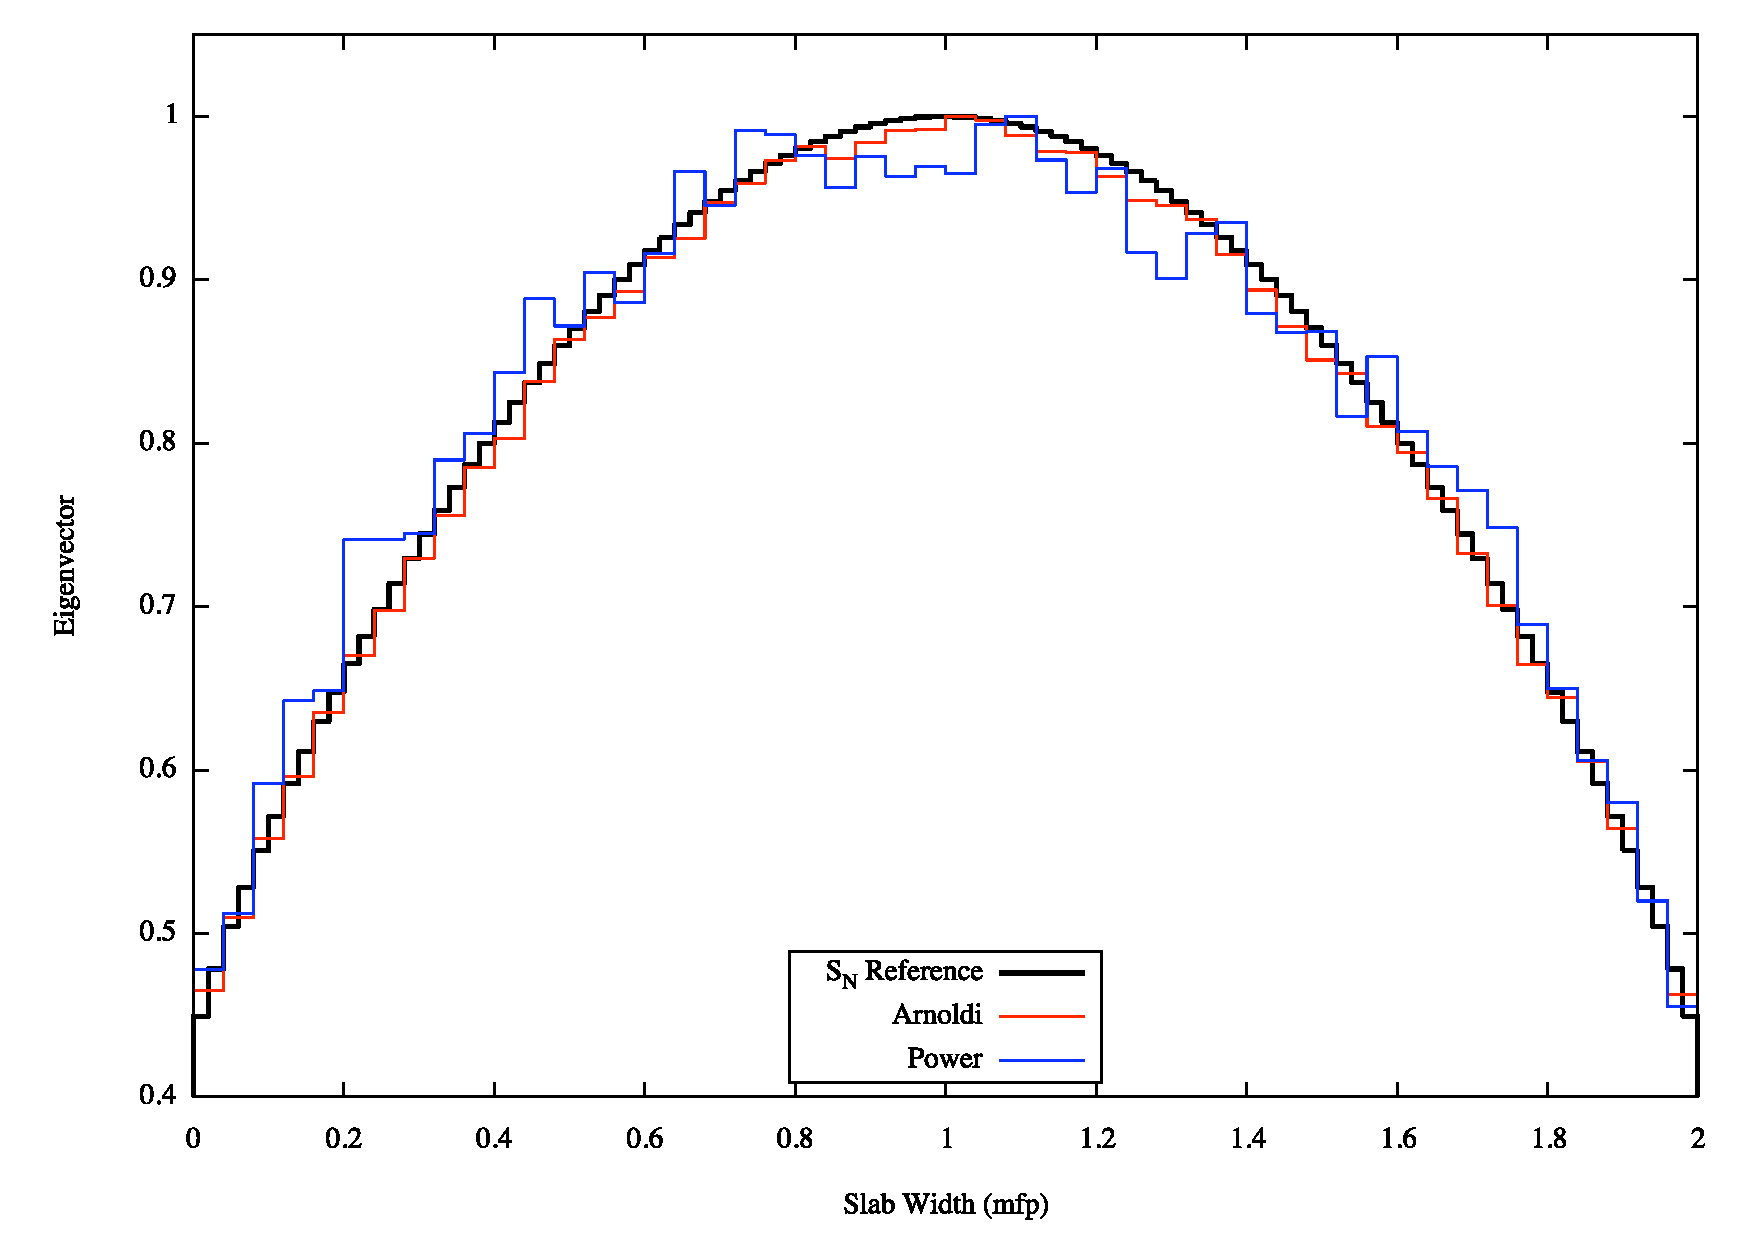
\includegraphics[width=\textwidth, keepaspectratio]{Arnoldi/Data/BasicFundamental-w2}
    % GNUPLOT: LaTeX picture with Postscript
\begingroup%
\makeatletter%
\newcommand{\GNUPLOTspecial}{%
  \@sanitize\catcode`\%=14\relax\special}%
\setlength{\unitlength}{0.0500bp}%
\begin{picture}(12960,8640)(0,0)%
  {\GNUPLOTspecial{"
%!PS-Adobe-2.0 EPSF-2.0
%%Title: BasicFundamental-w2.tex
%%Creator: gnuplot 4.3 patchlevel 0
%%CreationDate: Tue Jul 28 13:52:06 2009
%%DocumentFonts: 
%%BoundingBox: 0 0 648 432
%%EndComments
%%BeginProlog
/gnudict 256 dict def
gnudict begin
%
% The following true/false flags may be edited by hand if desired.
% The unit line width and grayscale image gamma correction may also be changed.
%
/Color true def
/Blacktext true def
/Solid true def
/Dashlength 1 def
/Landscape false def
/Level1 false def
/Rounded false def
/ClipToBoundingBox false def
/TransparentPatterns false def
/gnulinewidth 5.000 def
/userlinewidth gnulinewidth def
/Gamma 1.0 def
%
/vshift -66 def
/dl1 {
  10.0 Dashlength mul mul
  Rounded { currentlinewidth 0.75 mul sub dup 0 le { pop 0.01 } if } if
} def
/dl2 {
  10.0 Dashlength mul mul
  Rounded { currentlinewidth 0.75 mul add } if
} def
/hpt_ 31.5 def
/vpt_ 31.5 def
/hpt hpt_ def
/vpt vpt_ def
Level1 {} {
/SDict 10 dict def
systemdict /pdfmark known not {
  userdict /pdfmark systemdict /cleartomark get put
} if
SDict begin [
  /Title (BasicFundamental-w2.tex)
  /Subject (gnuplot plot)
  /Creator (gnuplot 4.3 patchlevel 0)
  /Author (Jeremy Conlin)
%  /Producer (gnuplot)
%  /Keywords ()
  /CreationDate (Tue Jul 28 13:52:06 2009)
  /DOCINFO pdfmark
end
} ifelse
/doclip {
  ClipToBoundingBox {
    newpath 0 0 moveto 648 0 lineto 648 432 lineto 0 432 lineto closepath
    clip
  } if
} def
%
% Gnuplot Prolog Version 4.2 (November 2007)
%
/M {moveto} bind def
/L {lineto} bind def
/R {rmoveto} bind def
/V {rlineto} bind def
/N {newpath moveto} bind def
/Z {closepath} bind def
/C {setrgbcolor} bind def
/f {rlineto fill} bind def
/Gshow {show} def   % May be redefined later in the file to support UTF-8
/vpt2 vpt 2 mul def
/hpt2 hpt 2 mul def
/Lshow {currentpoint stroke M 0 vshift R 
	Blacktext {gsave 0 setgray show grestore} {show} ifelse} def
/Rshow {currentpoint stroke M dup stringwidth pop neg vshift R
	Blacktext {gsave 0 setgray show grestore} {show} ifelse} def
/Cshow {currentpoint stroke M dup stringwidth pop -2 div vshift R 
	Blacktext {gsave 0 setgray show grestore} {show} ifelse} def
/UP {dup vpt_ mul /vpt exch def hpt_ mul /hpt exch def
  /hpt2 hpt 2 mul def /vpt2 vpt 2 mul def} def
/DL {Color {setrgbcolor Solid {pop []} if 0 setdash}
 {pop pop pop 0 setgray Solid {pop []} if 0 setdash} ifelse} def
/BL {stroke userlinewidth 2 mul setlinewidth
	Rounded {1 setlinejoin 1 setlinecap} if} def
/AL {stroke userlinewidth 2 div setlinewidth
	Rounded {1 setlinejoin 1 setlinecap} if} def
/UL {dup gnulinewidth mul /userlinewidth exch def
	dup 1 lt {pop 1} if 10 mul /udl exch def} def
/PL {stroke userlinewidth setlinewidth
	Rounded {1 setlinejoin 1 setlinecap} if} def
% Default Line colors
/LCw {1 1 1} def
/LCb {0 0 0} def
/LCa {0 0 0} def
/LC0 {1 0 0} def
/LC1 {0 1 0} def
/LC2 {0 0 1} def
/LC3 {1 0 1} def
/LC4 {0 1 1} def
/LC5 {1 1 0} def
/LC6 {0 0 0} def
/LC7 {1 0.3 0} def
/LC8 {0.5 0.5 0.5} def
% Default Line Types
/LTw {PL [] 1 setgray} def
/LTb {BL [] LCb DL} def
/LTa {AL [1 udl mul 2 udl mul] 0 setdash LCa setrgbcolor} def
/LT0 {PL [] LC0 DL} def
/LT1 {PL [4 dl1 2 dl2] LC1 DL} def
/LT2 {PL [2 dl1 3 dl2] LC2 DL} def
/LT3 {PL [1 dl1 1.5 dl2] LC3 DL} def
/LT4 {PL [6 dl1 2 dl2 1 dl1 2 dl2] LC4 DL} def
/LT5 {PL [3 dl1 3 dl2 1 dl1 3 dl2] LC5 DL} def
/LT6 {PL [2 dl1 2 dl2 2 dl1 6 dl2] LC6 DL} def
/LT7 {PL [1 dl1 2 dl2 6 dl1 2 dl2 1 dl1 2 dl2] LC7 DL} def
/LT8 {PL [2 dl1 2 dl2 2 dl1 2 dl2 2 dl1 2 dl2 2 dl1 4 dl2] LC8 DL} def
/Pnt {stroke [] 0 setdash gsave 1 setlinecap M 0 0 V stroke grestore} def
/Dia {stroke [] 0 setdash 2 copy vpt add M
  hpt neg vpt neg V hpt vpt neg V
  hpt vpt V hpt neg vpt V closepath stroke
  Pnt} def
/Pls {stroke [] 0 setdash vpt sub M 0 vpt2 V
  currentpoint stroke M
  hpt neg vpt neg R hpt2 0 V stroke
 } def
/Box {stroke [] 0 setdash 2 copy exch hpt sub exch vpt add M
  0 vpt2 neg V hpt2 0 V 0 vpt2 V
  hpt2 neg 0 V closepath stroke
  Pnt} def
/Crs {stroke [] 0 setdash exch hpt sub exch vpt add M
  hpt2 vpt2 neg V currentpoint stroke M
  hpt2 neg 0 R hpt2 vpt2 V stroke} def
/TriU {stroke [] 0 setdash 2 copy vpt 1.12 mul add M
  hpt neg vpt -1.62 mul V
  hpt 2 mul 0 V
  hpt neg vpt 1.62 mul V closepath stroke
  Pnt} def
/Star {2 copy Pls Crs} def
/BoxF {stroke [] 0 setdash exch hpt sub exch vpt add M
  0 vpt2 neg V hpt2 0 V 0 vpt2 V
  hpt2 neg 0 V closepath fill} def
/TriUF {stroke [] 0 setdash vpt 1.12 mul add M
  hpt neg vpt -1.62 mul V
  hpt 2 mul 0 V
  hpt neg vpt 1.62 mul V closepath fill} def
/TriD {stroke [] 0 setdash 2 copy vpt 1.12 mul sub M
  hpt neg vpt 1.62 mul V
  hpt 2 mul 0 V
  hpt neg vpt -1.62 mul V closepath stroke
  Pnt} def
/TriDF {stroke [] 0 setdash vpt 1.12 mul sub M
  hpt neg vpt 1.62 mul V
  hpt 2 mul 0 V
  hpt neg vpt -1.62 mul V closepath fill} def
/DiaF {stroke [] 0 setdash vpt add M
  hpt neg vpt neg V hpt vpt neg V
  hpt vpt V hpt neg vpt V closepath fill} def
/Pent {stroke [] 0 setdash 2 copy gsave
  translate 0 hpt M 4 {72 rotate 0 hpt L} repeat
  closepath stroke grestore Pnt} def
/PentF {stroke [] 0 setdash gsave
  translate 0 hpt M 4 {72 rotate 0 hpt L} repeat
  closepath fill grestore} def
/Circle {stroke [] 0 setdash 2 copy
  hpt 0 360 arc stroke Pnt} def
/CircleF {stroke [] 0 setdash hpt 0 360 arc fill} def
/C0 {BL [] 0 setdash 2 copy moveto vpt 90 450 arc} bind def
/C1 {BL [] 0 setdash 2 copy moveto
	2 copy vpt 0 90 arc closepath fill
	vpt 0 360 arc closepath} bind def
/C2 {BL [] 0 setdash 2 copy moveto
	2 copy vpt 90 180 arc closepath fill
	vpt 0 360 arc closepath} bind def
/C3 {BL [] 0 setdash 2 copy moveto
	2 copy vpt 0 180 arc closepath fill
	vpt 0 360 arc closepath} bind def
/C4 {BL [] 0 setdash 2 copy moveto
	2 copy vpt 180 270 arc closepath fill
	vpt 0 360 arc closepath} bind def
/C5 {BL [] 0 setdash 2 copy moveto
	2 copy vpt 0 90 arc
	2 copy moveto
	2 copy vpt 180 270 arc closepath fill
	vpt 0 360 arc} bind def
/C6 {BL [] 0 setdash 2 copy moveto
	2 copy vpt 90 270 arc closepath fill
	vpt 0 360 arc closepath} bind def
/C7 {BL [] 0 setdash 2 copy moveto
	2 copy vpt 0 270 arc closepath fill
	vpt 0 360 arc closepath} bind def
/C8 {BL [] 0 setdash 2 copy moveto
	2 copy vpt 270 360 arc closepath fill
	vpt 0 360 arc closepath} bind def
/C9 {BL [] 0 setdash 2 copy moveto
	2 copy vpt 270 450 arc closepath fill
	vpt 0 360 arc closepath} bind def
/C10 {BL [] 0 setdash 2 copy 2 copy moveto vpt 270 360 arc closepath fill
	2 copy moveto
	2 copy vpt 90 180 arc closepath fill
	vpt 0 360 arc closepath} bind def
/C11 {BL [] 0 setdash 2 copy moveto
	2 copy vpt 0 180 arc closepath fill
	2 copy moveto
	2 copy vpt 270 360 arc closepath fill
	vpt 0 360 arc closepath} bind def
/C12 {BL [] 0 setdash 2 copy moveto
	2 copy vpt 180 360 arc closepath fill
	vpt 0 360 arc closepath} bind def
/C13 {BL [] 0 setdash 2 copy moveto
	2 copy vpt 0 90 arc closepath fill
	2 copy moveto
	2 copy vpt 180 360 arc closepath fill
	vpt 0 360 arc closepath} bind def
/C14 {BL [] 0 setdash 2 copy moveto
	2 copy vpt 90 360 arc closepath fill
	vpt 0 360 arc} bind def
/C15 {BL [] 0 setdash 2 copy vpt 0 360 arc closepath fill
	vpt 0 360 arc closepath} bind def
/Rec {newpath 4 2 roll moveto 1 index 0 rlineto 0 exch rlineto
	neg 0 rlineto closepath} bind def
/Square {dup Rec} bind def
/Bsquare {vpt sub exch vpt sub exch vpt2 Square} bind def
/S0 {BL [] 0 setdash 2 copy moveto 0 vpt rlineto BL Bsquare} bind def
/S1 {BL [] 0 setdash 2 copy vpt Square fill Bsquare} bind def
/S2 {BL [] 0 setdash 2 copy exch vpt sub exch vpt Square fill Bsquare} bind def
/S3 {BL [] 0 setdash 2 copy exch vpt sub exch vpt2 vpt Rec fill Bsquare} bind def
/S4 {BL [] 0 setdash 2 copy exch vpt sub exch vpt sub vpt Square fill Bsquare} bind def
/S5 {BL [] 0 setdash 2 copy 2 copy vpt Square fill
	exch vpt sub exch vpt sub vpt Square fill Bsquare} bind def
/S6 {BL [] 0 setdash 2 copy exch vpt sub exch vpt sub vpt vpt2 Rec fill Bsquare} bind def
/S7 {BL [] 0 setdash 2 copy exch vpt sub exch vpt sub vpt vpt2 Rec fill
	2 copy vpt Square fill Bsquare} bind def
/S8 {BL [] 0 setdash 2 copy vpt sub vpt Square fill Bsquare} bind def
/S9 {BL [] 0 setdash 2 copy vpt sub vpt vpt2 Rec fill Bsquare} bind def
/S10 {BL [] 0 setdash 2 copy vpt sub vpt Square fill 2 copy exch vpt sub exch vpt Square fill
	Bsquare} bind def
/S11 {BL [] 0 setdash 2 copy vpt sub vpt Square fill 2 copy exch vpt sub exch vpt2 vpt Rec fill
	Bsquare} bind def
/S12 {BL [] 0 setdash 2 copy exch vpt sub exch vpt sub vpt2 vpt Rec fill Bsquare} bind def
/S13 {BL [] 0 setdash 2 copy exch vpt sub exch vpt sub vpt2 vpt Rec fill
	2 copy vpt Square fill Bsquare} bind def
/S14 {BL [] 0 setdash 2 copy exch vpt sub exch vpt sub vpt2 vpt Rec fill
	2 copy exch vpt sub exch vpt Square fill Bsquare} bind def
/S15 {BL [] 0 setdash 2 copy Bsquare fill Bsquare} bind def
/D0 {gsave translate 45 rotate 0 0 S0 stroke grestore} bind def
/D1 {gsave translate 45 rotate 0 0 S1 stroke grestore} bind def
/D2 {gsave translate 45 rotate 0 0 S2 stroke grestore} bind def
/D3 {gsave translate 45 rotate 0 0 S3 stroke grestore} bind def
/D4 {gsave translate 45 rotate 0 0 S4 stroke grestore} bind def
/D5 {gsave translate 45 rotate 0 0 S5 stroke grestore} bind def
/D6 {gsave translate 45 rotate 0 0 S6 stroke grestore} bind def
/D7 {gsave translate 45 rotate 0 0 S7 stroke grestore} bind def
/D8 {gsave translate 45 rotate 0 0 S8 stroke grestore} bind def
/D9 {gsave translate 45 rotate 0 0 S9 stroke grestore} bind def
/D10 {gsave translate 45 rotate 0 0 S10 stroke grestore} bind def
/D11 {gsave translate 45 rotate 0 0 S11 stroke grestore} bind def
/D12 {gsave translate 45 rotate 0 0 S12 stroke grestore} bind def
/D13 {gsave translate 45 rotate 0 0 S13 stroke grestore} bind def
/D14 {gsave translate 45 rotate 0 0 S14 stroke grestore} bind def
/D15 {gsave translate 45 rotate 0 0 S15 stroke grestore} bind def
/DiaE {stroke [] 0 setdash vpt add M
  hpt neg vpt neg V hpt vpt neg V
  hpt vpt V hpt neg vpt V closepath stroke} def
/BoxE {stroke [] 0 setdash exch hpt sub exch vpt add M
  0 vpt2 neg V hpt2 0 V 0 vpt2 V
  hpt2 neg 0 V closepath stroke} def
/TriUE {stroke [] 0 setdash vpt 1.12 mul add M
  hpt neg vpt -1.62 mul V
  hpt 2 mul 0 V
  hpt neg vpt 1.62 mul V closepath stroke} def
/TriDE {stroke [] 0 setdash vpt 1.12 mul sub M
  hpt neg vpt 1.62 mul V
  hpt 2 mul 0 V
  hpt neg vpt -1.62 mul V closepath stroke} def
/PentE {stroke [] 0 setdash gsave
  translate 0 hpt M 4 {72 rotate 0 hpt L} repeat
  closepath stroke grestore} def
/CircE {stroke [] 0 setdash 
  hpt 0 360 arc stroke} def
/Opaque {gsave closepath 1 setgray fill grestore 0 setgray closepath} def
/DiaW {stroke [] 0 setdash vpt add M
  hpt neg vpt neg V hpt vpt neg V
  hpt vpt V hpt neg vpt V Opaque stroke} def
/BoxW {stroke [] 0 setdash exch hpt sub exch vpt add M
  0 vpt2 neg V hpt2 0 V 0 vpt2 V
  hpt2 neg 0 V Opaque stroke} def
/TriUW {stroke [] 0 setdash vpt 1.12 mul add M
  hpt neg vpt -1.62 mul V
  hpt 2 mul 0 V
  hpt neg vpt 1.62 mul V Opaque stroke} def
/TriDW {stroke [] 0 setdash vpt 1.12 mul sub M
  hpt neg vpt 1.62 mul V
  hpt 2 mul 0 V
  hpt neg vpt -1.62 mul V Opaque stroke} def
/PentW {stroke [] 0 setdash gsave
  translate 0 hpt M 4 {72 rotate 0 hpt L} repeat
  Opaque stroke grestore} def
/CircW {stroke [] 0 setdash 
  hpt 0 360 arc Opaque stroke} def
/BoxFill {gsave Rec 1 setgray fill grestore} def
/Density {
  /Fillden exch def
  currentrgbcolor
  /ColB exch def /ColG exch def /ColR exch def
  /ColR ColR Fillden mul Fillden sub 1 add def
  /ColG ColG Fillden mul Fillden sub 1 add def
  /ColB ColB Fillden mul Fillden sub 1 add def
  ColR ColG ColB setrgbcolor} def
/BoxColFill {gsave Rec PolyFill} def
/PolyFill {gsave Density fill grestore grestore} def
/h {rlineto rlineto rlineto gsave closepath fill grestore} bind def
%
% PostScript Level 1 Pattern Fill routine for rectangles
% Usage: x y w h s a XX PatternFill
%	x,y = lower left corner of box to be filled
%	w,h = width and height of box
%	  a = angle in degrees between lines and x-axis
%	 XX = 0/1 for no/yes cross-hatch
%
/PatternFill {gsave /PFa [ 9 2 roll ] def
  PFa 0 get PFa 2 get 2 div add PFa 1 get PFa 3 get 2 div add translate
  PFa 2 get -2 div PFa 3 get -2 div PFa 2 get PFa 3 get Rec
  gsave 1 setgray fill grestore clip
  currentlinewidth 0.5 mul setlinewidth
  /PFs PFa 2 get dup mul PFa 3 get dup mul add sqrt def
  0 0 M PFa 5 get rotate PFs -2 div dup translate
  0 1 PFs PFa 4 get div 1 add floor cvi
	{PFa 4 get mul 0 M 0 PFs V} for
  0 PFa 6 get ne {
	0 1 PFs PFa 4 get div 1 add floor cvi
	{PFa 4 get mul 0 2 1 roll M PFs 0 V} for
 } if
  stroke grestore} def
%
/languagelevel where
 {pop languagelevel} {1} ifelse
 2 lt
	{/InterpretLevel1 true def}
	{/InterpretLevel1 Level1 def}
 ifelse
%
% PostScript level 2 pattern fill definitions
%
/Level2PatternFill {
/Tile8x8 {/PaintType 2 /PatternType 1 /TilingType 1 /BBox [0 0 8 8] /XStep 8 /YStep 8}
	bind def
/KeepColor {currentrgbcolor [/Pattern /DeviceRGB] setcolorspace} bind def
<< Tile8x8
 /PaintProc {0.5 setlinewidth pop 0 0 M 8 8 L 0 8 M 8 0 L stroke} 
>> matrix makepattern
/Pat1 exch def
<< Tile8x8
 /PaintProc {0.5 setlinewidth pop 0 0 M 8 8 L 0 8 M 8 0 L stroke
	0 4 M 4 8 L 8 4 L 4 0 L 0 4 L stroke}
>> matrix makepattern
/Pat2 exch def
<< Tile8x8
 /PaintProc {0.5 setlinewidth pop 0 0 M 0 8 L
	8 8 L 8 0 L 0 0 L fill}
>> matrix makepattern
/Pat3 exch def
<< Tile8x8
 /PaintProc {0.5 setlinewidth pop -4 8 M 8 -4 L
	0 12 M 12 0 L stroke}
>> matrix makepattern
/Pat4 exch def
<< Tile8x8
 /PaintProc {0.5 setlinewidth pop -4 0 M 8 12 L
	0 -4 M 12 8 L stroke}
>> matrix makepattern
/Pat5 exch def
<< Tile8x8
 /PaintProc {0.5 setlinewidth pop -2 8 M 4 -4 L
	0 12 M 8 -4 L 4 12 M 10 0 L stroke}
>> matrix makepattern
/Pat6 exch def
<< Tile8x8
 /PaintProc {0.5 setlinewidth pop -2 0 M 4 12 L
	0 -4 M 8 12 L 4 -4 M 10 8 L stroke}
>> matrix makepattern
/Pat7 exch def
<< Tile8x8
 /PaintProc {0.5 setlinewidth pop 8 -2 M -4 4 L
	12 0 M -4 8 L 12 4 M 0 10 L stroke}
>> matrix makepattern
/Pat8 exch def
<< Tile8x8
 /PaintProc {0.5 setlinewidth pop 0 -2 M 12 4 L
	-4 0 M 12 8 L -4 4 M 8 10 L stroke}
>> matrix makepattern
/Pat9 exch def
/Pattern1 {PatternBgnd KeepColor Pat1 setpattern} bind def
/Pattern2 {PatternBgnd KeepColor Pat2 setpattern} bind def
/Pattern3 {PatternBgnd KeepColor Pat3 setpattern} bind def
/Pattern4 {PatternBgnd KeepColor Landscape {Pat5} {Pat4} ifelse setpattern} bind def
/Pattern5 {PatternBgnd KeepColor Landscape {Pat4} {Pat5} ifelse setpattern} bind def
/Pattern6 {PatternBgnd KeepColor Landscape {Pat9} {Pat6} ifelse setpattern} bind def
/Pattern7 {PatternBgnd KeepColor Landscape {Pat8} {Pat7} ifelse setpattern} bind def
} def
%
%
%End of PostScript Level 2 code
%
/PatternBgnd {
  TransparentPatterns {} {gsave 1 setgray fill grestore} ifelse
} def
%
% Substitute for Level 2 pattern fill codes with
% grayscale if Level 2 support is not selected.
%
/Level1PatternFill {
/Pattern1 {0.250 Density} bind def
/Pattern2 {0.500 Density} bind def
/Pattern3 {0.750 Density} bind def
/Pattern4 {0.125 Density} bind def
/Pattern5 {0.375 Density} bind def
/Pattern6 {0.625 Density} bind def
/Pattern7 {0.875 Density} bind def
} def
%
% Now test for support of Level 2 code
%
Level1 {Level1PatternFill} {Level2PatternFill} ifelse
%
/Symbol-Oblique /Symbol findfont [1 0 .167 1 0 0] makefont
dup length dict begin {1 index /FID eq {pop pop} {def} ifelse} forall
currentdict end definefont pop
end
%%EndProlog
gnudict begin
gsave
doclip
0 0 translate
0.050 0.050 scale
0 setgray
newpath
1.000 UL
LTb
1100 640 M
63 0 V
11396 0 R
-63 0 V
1100 1834 M
63 0 V
11396 0 R
-63 0 V
1100 3027 M
63 0 V
11396 0 R
-63 0 V
1100 4221 M
63 0 V
11396 0 R
-63 0 V
1100 5415 M
63 0 V
11396 0 R
-63 0 V
1100 6608 M
63 0 V
11396 0 R
-63 0 V
1100 7802 M
63 0 V
11396 0 R
-63 0 V
1100 640 M
0 63 V
0 7696 R
0 -63 V
2246 640 M
0 63 V
0 7696 R
0 -63 V
3392 640 M
0 63 V
0 7696 R
0 -63 V
4538 640 M
0 63 V
0 7696 R
0 -63 V
5684 640 M
0 63 V
0 7696 R
0 -63 V
6830 640 M
0 63 V
0 7696 R
0 -63 V
7975 640 M
0 63 V
0 7696 R
0 -63 V
9121 640 M
0 63 V
0 7696 R
0 -63 V
10267 640 M
0 63 V
0 7696 R
0 -63 V
11413 640 M
0 63 V
0 7696 R
0 -63 V
12559 640 M
0 63 V
0 7696 R
0 -63 V
stroke
1100 8399 N
0 -7759 V
11459 0 V
0 7759 V
-11459 0 V
Z stroke
LCb setrgbcolor
LTb
LCb setrgbcolor
LTb
LCb setrgbcolor
LTb
LCb setrgbcolor
LTb
1.000 UP
1.000 UL
LTb
1.000 UL
LTb
5658 703 N
0 800 V
2342 0 V
0 -800 V
-2342 0 V
Z stroke
5658 1503 M
2342 0 V
stroke
2.000 UL
LTb
LCb setrgbcolor
LTb
7338 1303 M
543 0 V
1100 640 M
0 591 V
115 0 V
0 344 V
114 0 V
0 311 V
115 0 V
0 286 V
114 0 V
0 266 V
115 0 V
0 253 V
115 0 V
0 240 V
114 0 V
0 229 V
115 0 V
0 222 V
114 0 V
0 214 V
115 0 V
0 208 V
114 0 V
0 201 V
115 0 V
0 195 V
115 0 V
0 189 V
114 0 V
0 184 V
115 0 V
0 178 V
114 0 V
0 174 V
115 0 V
0 168 V
115 0 V
0 163 V
114 0 V
0 158 V
115 0 V
0 152 V
114 0 V
0 148 V
115 0 V
0 143 V
115 0 V
0 138 V
114 0 V
0 132 V
115 0 V
0 128 V
114 0 V
0 123 V
115 0 V
0 118 V
115 0 V
0 113 V
114 0 V
0 108 V
115 0 V
0 103 V
114 0 V
0 97 V
115 0 V
0 93 V
114 0 V
0 87 V
115 0 V
0 83 V
115 0 V
0 77 V
114 0 V
0 73 V
115 0 V
0 67 V
114 0 V
0 62 V
115 0 V
0 57 V
115 0 V
0 52 V
114 0 V
0 47 V
115 0 V
0 41 V
114 0 V
0 37 V
115 0 V
0 31 V
115 0 V
0 26 V
114 0 V
0 21 V
115 0 V
0 15 V
114 0 V
0 11 V
115 0 V
0 5 V
172 0 V
0 -5 V
172 0 V
stroke 7059 7797 M
0 -11 V
114 0 V
0 -15 V
115 0 V
0 -21 V
114 0 V
0 -26 V
115 0 V
0 -31 V
115 0 V
0 -37 V
114 0 V
0 -41 V
115 0 V
0 -47 V
114 0 V
0 -52 V
115 0 V
0 -57 V
115 0 V
0 -62 V
114 0 V
0 -67 V
115 0 V
0 -73 V
114 0 V
0 -77 V
115 0 V
0 -83 V
115 0 V
0 -87 V
114 0 V
0 -93 V
115 0 V
0 -97 V
114 0 V
0 -103 V
115 0 V
0 -108 V
114 0 V
0 -113 V
115 0 V
0 -118 V
115 0 V
0 -123 V
114 0 V
0 -128 V
115 0 V
0 -132 V
114 0 V
0 -138 V
115 0 V
0 -143 V
115 0 V
0 -148 V
114 0 V
0 -152 V
115 0 V
0 -158 V
114 0 V
0 -163 V
115 0 V
0 -168 V
115 0 V
0 -174 V
114 0 V
0 -178 V
115 0 V
0 -184 V
114 0 V
0 -189 V
115 0 V
0 -195 V
115 0 V
0 -201 V
114 0 V
0 -208 V
115 0 V
0 -214 V
114 0 V
0 -222 V
115 0 V
0 -229 V
114 0 V
0 -240 V
115 0 V
0 -253 V
115 0 V
0 -266 V
114 0 V
0 -286 V
115 0 V
0 -311 V
114 0 V
0 -344 V
115 0 V
0 -591 V
stroke
1.000 UL
LT0
LCb setrgbcolor
LT0
7338 1103 M
543 0 V
1100 1318 M
153 0 V
0 446 V
153 0 V
0 371 V
152 0 V
0 338 V
153 0 V
0 332 V
153 0 V
0 309 V
153 0 V
0 320 V
152 0 V
0 277 V
153 0 V
0 261 V
153 0 V
0 266 V
153 0 V
0 255 V
153 0 V
0 218 V
152 0 V
0 250 V
153 0 V
0 215 V
153 0 V
0 216 V
153 0 V
0 197 V
153 0 V
0 216 V
152 0 V
0 175 V
153 0 V
0 178 V
153 0 V
0 169 V
153 0 V
0 141 V
153 0 V
0 166 V
152 0 V
0 135 V
153 0 V
0 133 V
153 0 V
0 116 V
153 0 V
0 145 V
152 0 V
0 83 V
153 0 V
0 102 V
153 0 V
0 73 V
153 0 V
0 92 V
153 0 V
0 80 V
152 0 V
0 63 V
153 0 V
0 46 V
153 0 V
0 51 V
153 0 V
0 31 V
153 0 V
0 1 V
152 0 V
0 14 V
153 0 V
0 3 V
153 0 V
0 -7 V
153 0 V
0 -5 V
152 0 V
0 -23 V
153 0 V
0 -25 V
153 0 V
0 -44 V
153 0 V
0 -57 V
153 0 V
0 -65 V
152 0 V
0 -72 V
153 0 V
0 -63 V
153 0 V
0 -102 V
153 0 V
0 -93 V
152 0 V
0 -110 V
153 0 V
0 -90 V
153 0 V
0 -134 V
stroke 8892 6912 M
153 0 V
0 -131 V
153 0 V
0 -163 V
152 0 V
0 -159 V
153 0 V
0 -131 V
153 0 V
0 -180 V
153 0 V
0 -175 V
153 0 V
0 -177 V
153 0 V
0 -206 V
152 0 V
0 -192 V
153 0 V
0 -210 V
153 0 V
0 -234 V
153 0 V
0 -240 V
152 0 V
0 -222 V
153 0 V
0 -261 V
153 0 V
0 -250 V
153 0 V
0 -279 V
153 0 V
0 -289 V
152 0 V
0 -288 V
153 0 V
0 -299 V
153 0 V
0 -326 V
153 0 V
0 -354 V
152 0 V
0 -390 V
153 0 V
0 -431 V
153 0 V
stroke
LT2
LCb setrgbcolor
LT2
7338 903 M
543 0 V
1100 1304 M
153 0 V
0 435 V
153 0 V
0 372 V
152 0 V
0 380 V
153 0 V
0 305 V
153 0 V
0 304 V
153 0 V
0 294 V
152 0 V
0 290 V
153 0 V
0 261 V
153 0 V
0 284 V
153 0 V
0 251 V
153 0 V
0 219 V
152 0 V
0 231 V
153 0 V
0 223 V
153 0 V
0 220 V
153 0 V
0 182 V
153 0 V
0 242 V
152 0 V
0 188 V
153 0 V
0 131 V
153 0 V
0 205 V
153 0 V
0 153 V
153 0 V
0 122 V
152 0 V
0 163 V
153 0 V
0 84 V
153 0 V
0 164 V
153 0 V
0 111 V
152 0 V
0 95 V
153 0 V
0 142 V
153 0 V
0 41 V
153 0 V
0 84 V
153 0 V
0 79 V
152 0 V
0 43 V
153 0 V
0 78 V
153 0 V
0 1 V
153 0 V
0 65 V
153 0 V
0 29 V
152 0 V
0 5 V
153 0 V
0 22 V
153 0 V
0 -19 V
153 0 V
152 0 V
0 -42 V
153 0 V
0 -42 V
153 0 V
0 -19 V
153 0 V
0 -90 V
153 0 V
0 -33 V
152 0 V
0 -66 V
153 0 V
0 -64 V
153 0 V
0 -80 V
153 0 V
0 -132 V
152 0 V
0 -83 V
153 0 V
0 -106 V
153 0 V
0 -127 V
153 0 V
stroke 9045 6899 M
0 -115 V
153 0 V
0 -167 V
152 0 V
0 -170 V
153 0 V
0 -148 V
153 0 V
0 -169 V
153 0 V
0 -208 V
153 0 V
0 -174 V
153 0 V
0 -198 V
152 0 V
0 -165 V
153 0 V
0 -206 V
153 0 V
0 -207 V
153 0 V
0 -287 V
152 0 V
0 -211 V
153 0 V
0 -250 V
153 0 V
0 -264 V
153 0 V
0 -261 V
153 0 V
0 -278 V
152 0 V
0 -313 V
153 0 V
0 -299 V
153 0 V
0 -312 V
153 0 V
0 -347 V
152 0 V
0 -411 V
153 0 V
0 -416 V
153 0 V
stroke
LTb
1100 8399 N
0 -7759 V
11459 0 V
0 7759 V
-11459 0 V
Z stroke
1.000 UP
1.000 UL
LTb
stroke
grestore
end
showpage
  }}%
  \put(7218,903){\makebox(0,0)[r]{\strut{}Arnoldi}}%
  \put(7218,1103){\makebox(0,0)[r]{\strut{}Power}}%
  \put(7218,1303){\makebox(0,0)[r]{\strut{}$S_N$ Reference}}%
  \put(6829,140){\makebox(0,0){\strut{}Slab Width (mfp)}}%
  \put(280,4519){%
  \special{ps: gsave currentpoint currentpoint translate
270 rotate neg exch neg exch translate}%
  \makebox(0,0){\strut{}Eigenvector}%
  \special{ps: currentpoint grestore moveto}%
  }%
  \put(12559,440){\makebox(0,0){\strut{} 2}}%
  \put(11413,440){\makebox(0,0){\strut{} 1.8}}%
  \put(10267,440){\makebox(0,0){\strut{} 1.6}}%
  \put(9121,440){\makebox(0,0){\strut{} 1.4}}%
  \put(7975,440){\makebox(0,0){\strut{} 1.2}}%
  \put(6830,440){\makebox(0,0){\strut{} 1}}%
  \put(5684,440){\makebox(0,0){\strut{} 0.8}}%
  \put(4538,440){\makebox(0,0){\strut{} 0.6}}%
  \put(3392,440){\makebox(0,0){\strut{} 0.4}}%
  \put(2246,440){\makebox(0,0){\strut{} 0.2}}%
  \put(1100,440){\makebox(0,0){\strut{} 0}}%
  \put(980,7802){\makebox(0,0)[r]{\strut{} 1}}%
  \put(980,6608){\makebox(0,0)[r]{\strut{} 0.9}}%
  \put(980,5415){\makebox(0,0)[r]{\strut{} 0.8}}%
  \put(980,4221){\makebox(0,0)[r]{\strut{} 0.7}}%
  \put(980,3027){\makebox(0,0)[r]{\strut{} 0.6}}%
  \put(980,1834){\makebox(0,0)[r]{\strut{} 0.5}}%
  \put(980,640){\makebox(0,0)[r]{\strut{} 0.4}}%
\end{picture}%
\endgroup
\endinput

    \caption{Fundamental eigenvector estimates from the power method and Arnoldi's method for the 2.0 mfp wide slab.  The heavy line shows the S$_\mathrm{N}$ solution.}
    \label{fig:BasicFundamentalW2}
\end{sidewaysfigure}
\end{comment}

\clearpage
\subsection{Discretization Error \label{sec:DiscretizationBias}} 

One of the benefits of Monte Carlo particle transport is the ability to use exact geometry without discretization.  This is true for the transport of particles in the power method, but the fission source must be discretized for tallying.  Arnoldi's method, on the other hand, must have a discretized source  in order to orthogonalize the Arnoldi vectors, as described in \Fref{sec:SpatialDiscretization}.

The discretization of the fission source can lead to an error in the estimated eigenvalue if an insufficient number of spatial bins are used to represent the fission source.  To illustrate this effect a series of simulations is shown using the same slab of multiplying material with varying number of spatial bins.  The slab here is exactly the same as for the 20 mfp problem shown earlier (\mbox{$\nu\Sigma_f = 1.0$}, \mbox{$\Sigma_a = 0.2$}, \mbox{$\Sigma_s = 0.8$} with \mbox{$\Sigma_t = 1.0$}).  This time $10^5$ histories are tracked per iteration with 50 inactive restarts and 500 active restarts.  The increase in the number of histories and restarts is to reduce the statistical uncertainty to ensure the error can be seen outside the noise.  This simulation was performed eleven times varying the number of spatial discretization bins from 10 to 150.  

The results of these simulations are shown in \Fref{tab:Discretization} for the fundamental eigenvalue.  We can see that the uncertainty in the eigenvalue estimate (standard deviation) is relatively independent of the number of spatial bins.  The error in the eigenvalue estimate is the absolute value of the difference between the eigenvalue estimate and the reference solution.  We see that the error in the eigenvalue estimate is larger than the statistical uncertainty for bin widths \mbox{$\leq 0.5$} mfp thick.  For bin widths greater than 0.5 mfp thick the error is less than the statistical uncertainty. 

The data from \Fref{tab:Discretization} is shown graphically in \Fref{fig:BasicBias}.  The error in the eigenvalue estimate for the first two harmonics are also shown in \Fref{fig:BasicBias}.  The error in the eigenvalue estimate is denoted marked as $\mathcal{B}$ for each of the eigenvalue estimates.  Best fit lines are drawn through the points on the graph.  We see that there is a very good linear fit to these data points.  

\begin{table}[h] \centering
    \begin{tabular}{cccccc}
        \toprule
        \# of Bins & Bin Width (mfp) & Eigenvalue & Uncertainty & Error & FOM\\
        \midrule
         10 & 2.00 & 4.8003 & 6.6\e{-4} & 2.7\e{-2} & 831.2 \\
         25 & 0.80 & 4.8224 & 6.8\e{-4} & 5.3\e{-3} & 773.2 \\
         40 & 0.50 & 4.8251 & 6.3\e{-4} & 2.6\e{-3} & 872.0 \\
         50 & 0.40 & 4.8273 & 6.5\e{-4} & 4.2\e{-4} & 829.0 \\
         60 & 0.33 & 4.8258 & 6.9\e{-4} & 2.0\e{-3} & 704.3 \\
         75 & 0.27 & 4.8275 & 6.7\e{-4} & 2.4\e{-4} & 753.0 \\
         90 & 0.22 & 4.8277 & 6.7\e{-4} & 4.2\e{-5} & 746.1 \\
        105 & 0.19 & 4.8277 & 6.9\e{-4} & 5.2\e{-5} & 698.3 \\
        120 & 0.17 & 4.8282 & 6.5\e{-4} & 4.1\e{-4} & 767.8 \\
        135 & 0.15 & 4.8274 & 7.0\e{-4} & 3.1\e{-4} & 656.9 \\
        150 & 0.13 & 4.8285 & 6.4\e{-4} & 7.5\e{-4} & 792.0 \\
        \bottomrule
    \end{tabular}
    \caption{Eigenvalue estimates of the fundamental eigenvalue from Arnoldi's method and the error in the estimate.  The error is the difference between the estimate and the reference value ($\lambda_0 = 4.8278$, see \cite{Garis:1991One-s-0} and \cite{Dahl:1979Eigen-0}).}
    \label{tab:Discretization}
\end{table}

\begin{sidewaysfigure}[h] \centering
    % GNUPLOT: LaTeX picture with Postscript
\begingroup%
\makeatletter%
\newcommand{\GNUPLOTspecial}{%
  \@sanitize\catcode`\%=14\relax\special}%
\setlength{\unitlength}{0.0500bp}%
\begin{picture}(8640,6480)(0,0)%
  {\GNUPLOTspecial{"
%!PS-Adobe-2.0 EPSF-2.0
%%Title: BiasHistogram.tex
%%Creator: gnuplot 4.3 patchlevel 0
%%CreationDate: Wed Aug 12 16:28:22 2009
%%DocumentFonts: 
%%BoundingBox: 0 0 432 324
%%EndComments
%%BeginProlog
/gnudict 256 dict def
gnudict begin
%
% The following true/false flags may be edited by hand if desired.
% The unit line width and grayscale image gamma correction may also be changed.
%
/Color true def
/Blacktext true def
/Solid true def
/Dashlength 1 def
/Landscape false def
/Level1 false def
/Rounded false def
/ClipToBoundingBox false def
/TransparentPatterns false def
/gnulinewidth 5.000 def
/userlinewidth gnulinewidth def
/Gamma 1.0 def
%
/vshift -66 def
/dl1 {
  10.0 Dashlength mul mul
  Rounded { currentlinewidth 0.75 mul sub dup 0 le { pop 0.01 } if } if
} def
/dl2 {
  10.0 Dashlength mul mul
  Rounded { currentlinewidth 0.75 mul add } if
} def
/hpt_ 31.5 def
/vpt_ 31.5 def
/hpt hpt_ def
/vpt vpt_ def
Level1 {} {
/SDict 10 dict def
systemdict /pdfmark known not {
  userdict /pdfmark systemdict /cleartomark get put
} if
SDict begin [
  /Title (BiasHistogram.tex)
  /Subject (gnuplot plot)
  /Creator (gnuplot 4.3 patchlevel 0)
  /Author (Jeremy Conlin)
%  /Producer (gnuplot)
%  /Keywords ()
  /CreationDate (Wed Aug 12 16:28:22 2009)
  /DOCINFO pdfmark
end
} ifelse
/doclip {
  ClipToBoundingBox {
    newpath 0 0 moveto 432 0 lineto 432 324 lineto 0 324 lineto closepath
    clip
  } if
} def
%
% Gnuplot Prolog Version 4.2 (November 2007)
%
/M {moveto} bind def
/L {lineto} bind def
/R {rmoveto} bind def
/V {rlineto} bind def
/N {newpath moveto} bind def
/Z {closepath} bind def
/C {setrgbcolor} bind def
/f {rlineto fill} bind def
/Gshow {show} def   % May be redefined later in the file to support UTF-8
/vpt2 vpt 2 mul def
/hpt2 hpt 2 mul def
/Lshow {currentpoint stroke M 0 vshift R 
	Blacktext {gsave 0 setgray show grestore} {show} ifelse} def
/Rshow {currentpoint stroke M dup stringwidth pop neg vshift R
	Blacktext {gsave 0 setgray show grestore} {show} ifelse} def
/Cshow {currentpoint stroke M dup stringwidth pop -2 div vshift R 
	Blacktext {gsave 0 setgray show grestore} {show} ifelse} def
/UP {dup vpt_ mul /vpt exch def hpt_ mul /hpt exch def
  /hpt2 hpt 2 mul def /vpt2 vpt 2 mul def} def
/DL {Color {setrgbcolor Solid {pop []} if 0 setdash}
 {pop pop pop 0 setgray Solid {pop []} if 0 setdash} ifelse} def
/BL {stroke userlinewidth 2 mul setlinewidth
	Rounded {1 setlinejoin 1 setlinecap} if} def
/AL {stroke userlinewidth 2 div setlinewidth
	Rounded {1 setlinejoin 1 setlinecap} if} def
/UL {dup gnulinewidth mul /userlinewidth exch def
	dup 1 lt {pop 1} if 10 mul /udl exch def} def
/PL {stroke userlinewidth setlinewidth
	Rounded {1 setlinejoin 1 setlinecap} if} def
% Default Line colors
/LCw {1 1 1} def
/LCb {0 0 0} def
/LCa {0 0 0} def
/LC0 {1 0 0} def
/LC1 {0 1 0} def
/LC2 {0 0 1} def
/LC3 {1 0 1} def
/LC4 {0 1 1} def
/LC5 {1 1 0} def
/LC6 {0 0 0} def
/LC7 {1 0.3 0} def
/LC8 {0.5 0.5 0.5} def
% Default Line Types
/LTw {PL [] 1 setgray} def
/LTb {BL [] LCb DL} def
/LTa {AL [1 udl mul 2 udl mul] 0 setdash LCa setrgbcolor} def
/LT0 {PL [] LC0 DL} def
/LT1 {PL [4 dl1 2 dl2] LC1 DL} def
/LT2 {PL [2 dl1 3 dl2] LC2 DL} def
/LT3 {PL [1 dl1 1.5 dl2] LC3 DL} def
/LT4 {PL [6 dl1 2 dl2 1 dl1 2 dl2] LC4 DL} def
/LT5 {PL [3 dl1 3 dl2 1 dl1 3 dl2] LC5 DL} def
/LT6 {PL [2 dl1 2 dl2 2 dl1 6 dl2] LC6 DL} def
/LT7 {PL [1 dl1 2 dl2 6 dl1 2 dl2 1 dl1 2 dl2] LC7 DL} def
/LT8 {PL [2 dl1 2 dl2 2 dl1 2 dl2 2 dl1 2 dl2 2 dl1 4 dl2] LC8 DL} def
/Pnt {stroke [] 0 setdash gsave 1 setlinecap M 0 0 V stroke grestore} def
/Dia {stroke [] 0 setdash 2 copy vpt add M
  hpt neg vpt neg V hpt vpt neg V
  hpt vpt V hpt neg vpt V closepath stroke
  Pnt} def
/Pls {stroke [] 0 setdash vpt sub M 0 vpt2 V
  currentpoint stroke M
  hpt neg vpt neg R hpt2 0 V stroke
 } def
/Box {stroke [] 0 setdash 2 copy exch hpt sub exch vpt add M
  0 vpt2 neg V hpt2 0 V 0 vpt2 V
  hpt2 neg 0 V closepath stroke
  Pnt} def
/Crs {stroke [] 0 setdash exch hpt sub exch vpt add M
  hpt2 vpt2 neg V currentpoint stroke M
  hpt2 neg 0 R hpt2 vpt2 V stroke} def
/TriU {stroke [] 0 setdash 2 copy vpt 1.12 mul add M
  hpt neg vpt -1.62 mul V
  hpt 2 mul 0 V
  hpt neg vpt 1.62 mul V closepath stroke
  Pnt} def
/Star {2 copy Pls Crs} def
/BoxF {stroke [] 0 setdash exch hpt sub exch vpt add M
  0 vpt2 neg V hpt2 0 V 0 vpt2 V
  hpt2 neg 0 V closepath fill} def
/TriUF {stroke [] 0 setdash vpt 1.12 mul add M
  hpt neg vpt -1.62 mul V
  hpt 2 mul 0 V
  hpt neg vpt 1.62 mul V closepath fill} def
/TriD {stroke [] 0 setdash 2 copy vpt 1.12 mul sub M
  hpt neg vpt 1.62 mul V
  hpt 2 mul 0 V
  hpt neg vpt -1.62 mul V closepath stroke
  Pnt} def
/TriDF {stroke [] 0 setdash vpt 1.12 mul sub M
  hpt neg vpt 1.62 mul V
  hpt 2 mul 0 V
  hpt neg vpt -1.62 mul V closepath fill} def
/DiaF {stroke [] 0 setdash vpt add M
  hpt neg vpt neg V hpt vpt neg V
  hpt vpt V hpt neg vpt V closepath fill} def
/Pent {stroke [] 0 setdash 2 copy gsave
  translate 0 hpt M 4 {72 rotate 0 hpt L} repeat
  closepath stroke grestore Pnt} def
/PentF {stroke [] 0 setdash gsave
  translate 0 hpt M 4 {72 rotate 0 hpt L} repeat
  closepath fill grestore} def
/Circle {stroke [] 0 setdash 2 copy
  hpt 0 360 arc stroke Pnt} def
/CircleF {stroke [] 0 setdash hpt 0 360 arc fill} def
/C0 {BL [] 0 setdash 2 copy moveto vpt 90 450 arc} bind def
/C1 {BL [] 0 setdash 2 copy moveto
	2 copy vpt 0 90 arc closepath fill
	vpt 0 360 arc closepath} bind def
/C2 {BL [] 0 setdash 2 copy moveto
	2 copy vpt 90 180 arc closepath fill
	vpt 0 360 arc closepath} bind def
/C3 {BL [] 0 setdash 2 copy moveto
	2 copy vpt 0 180 arc closepath fill
	vpt 0 360 arc closepath} bind def
/C4 {BL [] 0 setdash 2 copy moveto
	2 copy vpt 180 270 arc closepath fill
	vpt 0 360 arc closepath} bind def
/C5 {BL [] 0 setdash 2 copy moveto
	2 copy vpt 0 90 arc
	2 copy moveto
	2 copy vpt 180 270 arc closepath fill
	vpt 0 360 arc} bind def
/C6 {BL [] 0 setdash 2 copy moveto
	2 copy vpt 90 270 arc closepath fill
	vpt 0 360 arc closepath} bind def
/C7 {BL [] 0 setdash 2 copy moveto
	2 copy vpt 0 270 arc closepath fill
	vpt 0 360 arc closepath} bind def
/C8 {BL [] 0 setdash 2 copy moveto
	2 copy vpt 270 360 arc closepath fill
	vpt 0 360 arc closepath} bind def
/C9 {BL [] 0 setdash 2 copy moveto
	2 copy vpt 270 450 arc closepath fill
	vpt 0 360 arc closepath} bind def
/C10 {BL [] 0 setdash 2 copy 2 copy moveto vpt 270 360 arc closepath fill
	2 copy moveto
	2 copy vpt 90 180 arc closepath fill
	vpt 0 360 arc closepath} bind def
/C11 {BL [] 0 setdash 2 copy moveto
	2 copy vpt 0 180 arc closepath fill
	2 copy moveto
	2 copy vpt 270 360 arc closepath fill
	vpt 0 360 arc closepath} bind def
/C12 {BL [] 0 setdash 2 copy moveto
	2 copy vpt 180 360 arc closepath fill
	vpt 0 360 arc closepath} bind def
/C13 {BL [] 0 setdash 2 copy moveto
	2 copy vpt 0 90 arc closepath fill
	2 copy moveto
	2 copy vpt 180 360 arc closepath fill
	vpt 0 360 arc closepath} bind def
/C14 {BL [] 0 setdash 2 copy moveto
	2 copy vpt 90 360 arc closepath fill
	vpt 0 360 arc} bind def
/C15 {BL [] 0 setdash 2 copy vpt 0 360 arc closepath fill
	vpt 0 360 arc closepath} bind def
/Rec {newpath 4 2 roll moveto 1 index 0 rlineto 0 exch rlineto
	neg 0 rlineto closepath} bind def
/Square {dup Rec} bind def
/Bsquare {vpt sub exch vpt sub exch vpt2 Square} bind def
/S0 {BL [] 0 setdash 2 copy moveto 0 vpt rlineto BL Bsquare} bind def
/S1 {BL [] 0 setdash 2 copy vpt Square fill Bsquare} bind def
/S2 {BL [] 0 setdash 2 copy exch vpt sub exch vpt Square fill Bsquare} bind def
/S3 {BL [] 0 setdash 2 copy exch vpt sub exch vpt2 vpt Rec fill Bsquare} bind def
/S4 {BL [] 0 setdash 2 copy exch vpt sub exch vpt sub vpt Square fill Bsquare} bind def
/S5 {BL [] 0 setdash 2 copy 2 copy vpt Square fill
	exch vpt sub exch vpt sub vpt Square fill Bsquare} bind def
/S6 {BL [] 0 setdash 2 copy exch vpt sub exch vpt sub vpt vpt2 Rec fill Bsquare} bind def
/S7 {BL [] 0 setdash 2 copy exch vpt sub exch vpt sub vpt vpt2 Rec fill
	2 copy vpt Square fill Bsquare} bind def
/S8 {BL [] 0 setdash 2 copy vpt sub vpt Square fill Bsquare} bind def
/S9 {BL [] 0 setdash 2 copy vpt sub vpt vpt2 Rec fill Bsquare} bind def
/S10 {BL [] 0 setdash 2 copy vpt sub vpt Square fill 2 copy exch vpt sub exch vpt Square fill
	Bsquare} bind def
/S11 {BL [] 0 setdash 2 copy vpt sub vpt Square fill 2 copy exch vpt sub exch vpt2 vpt Rec fill
	Bsquare} bind def
/S12 {BL [] 0 setdash 2 copy exch vpt sub exch vpt sub vpt2 vpt Rec fill Bsquare} bind def
/S13 {BL [] 0 setdash 2 copy exch vpt sub exch vpt sub vpt2 vpt Rec fill
	2 copy vpt Square fill Bsquare} bind def
/S14 {BL [] 0 setdash 2 copy exch vpt sub exch vpt sub vpt2 vpt Rec fill
	2 copy exch vpt sub exch vpt Square fill Bsquare} bind def
/S15 {BL [] 0 setdash 2 copy Bsquare fill Bsquare} bind def
/D0 {gsave translate 45 rotate 0 0 S0 stroke grestore} bind def
/D1 {gsave translate 45 rotate 0 0 S1 stroke grestore} bind def
/D2 {gsave translate 45 rotate 0 0 S2 stroke grestore} bind def
/D3 {gsave translate 45 rotate 0 0 S3 stroke grestore} bind def
/D4 {gsave translate 45 rotate 0 0 S4 stroke grestore} bind def
/D5 {gsave translate 45 rotate 0 0 S5 stroke grestore} bind def
/D6 {gsave translate 45 rotate 0 0 S6 stroke grestore} bind def
/D7 {gsave translate 45 rotate 0 0 S7 stroke grestore} bind def
/D8 {gsave translate 45 rotate 0 0 S8 stroke grestore} bind def
/D9 {gsave translate 45 rotate 0 0 S9 stroke grestore} bind def
/D10 {gsave translate 45 rotate 0 0 S10 stroke grestore} bind def
/D11 {gsave translate 45 rotate 0 0 S11 stroke grestore} bind def
/D12 {gsave translate 45 rotate 0 0 S12 stroke grestore} bind def
/D13 {gsave translate 45 rotate 0 0 S13 stroke grestore} bind def
/D14 {gsave translate 45 rotate 0 0 S14 stroke grestore} bind def
/D15 {gsave translate 45 rotate 0 0 S15 stroke grestore} bind def
/DiaE {stroke [] 0 setdash vpt add M
  hpt neg vpt neg V hpt vpt neg V
  hpt vpt V hpt neg vpt V closepath stroke} def
/BoxE {stroke [] 0 setdash exch hpt sub exch vpt add M
  0 vpt2 neg V hpt2 0 V 0 vpt2 V
  hpt2 neg 0 V closepath stroke} def
/TriUE {stroke [] 0 setdash vpt 1.12 mul add M
  hpt neg vpt -1.62 mul V
  hpt 2 mul 0 V
  hpt neg vpt 1.62 mul V closepath stroke} def
/TriDE {stroke [] 0 setdash vpt 1.12 mul sub M
  hpt neg vpt 1.62 mul V
  hpt 2 mul 0 V
  hpt neg vpt -1.62 mul V closepath stroke} def
/PentE {stroke [] 0 setdash gsave
  translate 0 hpt M 4 {72 rotate 0 hpt L} repeat
  closepath stroke grestore} def
/CircE {stroke [] 0 setdash 
  hpt 0 360 arc stroke} def
/Opaque {gsave closepath 1 setgray fill grestore 0 setgray closepath} def
/DiaW {stroke [] 0 setdash vpt add M
  hpt neg vpt neg V hpt vpt neg V
  hpt vpt V hpt neg vpt V Opaque stroke} def
/BoxW {stroke [] 0 setdash exch hpt sub exch vpt add M
  0 vpt2 neg V hpt2 0 V 0 vpt2 V
  hpt2 neg 0 V Opaque stroke} def
/TriUW {stroke [] 0 setdash vpt 1.12 mul add M
  hpt neg vpt -1.62 mul V
  hpt 2 mul 0 V
  hpt neg vpt 1.62 mul V Opaque stroke} def
/TriDW {stroke [] 0 setdash vpt 1.12 mul sub M
  hpt neg vpt 1.62 mul V
  hpt 2 mul 0 V
  hpt neg vpt -1.62 mul V Opaque stroke} def
/PentW {stroke [] 0 setdash gsave
  translate 0 hpt M 4 {72 rotate 0 hpt L} repeat
  Opaque stroke grestore} def
/CircW {stroke [] 0 setdash 
  hpt 0 360 arc Opaque stroke} def
/BoxFill {gsave Rec 1 setgray fill grestore} def
/Density {
  /Fillden exch def
  currentrgbcolor
  /ColB exch def /ColG exch def /ColR exch def
  /ColR ColR Fillden mul Fillden sub 1 add def
  /ColG ColG Fillden mul Fillden sub 1 add def
  /ColB ColB Fillden mul Fillden sub 1 add def
  ColR ColG ColB setrgbcolor} def
/BoxColFill {gsave Rec PolyFill} def
/PolyFill {gsave Density fill grestore grestore} def
/h {rlineto rlineto rlineto gsave closepath fill grestore} bind def
%
% PostScript Level 1 Pattern Fill routine for rectangles
% Usage: x y w h s a XX PatternFill
%	x,y = lower left corner of box to be filled
%	w,h = width and height of box
%	  a = angle in degrees between lines and x-axis
%	 XX = 0/1 for no/yes cross-hatch
%
/PatternFill {gsave /PFa [ 9 2 roll ] def
  PFa 0 get PFa 2 get 2 div add PFa 1 get PFa 3 get 2 div add translate
  PFa 2 get -2 div PFa 3 get -2 div PFa 2 get PFa 3 get Rec
  gsave 1 setgray fill grestore clip
  currentlinewidth 0.5 mul setlinewidth
  /PFs PFa 2 get dup mul PFa 3 get dup mul add sqrt def
  0 0 M PFa 5 get rotate PFs -2 div dup translate
  0 1 PFs PFa 4 get div 1 add floor cvi
	{PFa 4 get mul 0 M 0 PFs V} for
  0 PFa 6 get ne {
	0 1 PFs PFa 4 get div 1 add floor cvi
	{PFa 4 get mul 0 2 1 roll M PFs 0 V} for
 } if
  stroke grestore} def
%
/languagelevel where
 {pop languagelevel} {1} ifelse
 2 lt
	{/InterpretLevel1 true def}
	{/InterpretLevel1 Level1 def}
 ifelse
%
% PostScript level 2 pattern fill definitions
%
/Level2PatternFill {
/Tile8x8 {/PaintType 2 /PatternType 1 /TilingType 1 /BBox [0 0 8 8] /XStep 8 /YStep 8}
	bind def
/KeepColor {currentrgbcolor [/Pattern /DeviceRGB] setcolorspace} bind def
<< Tile8x8
 /PaintProc {0.5 setlinewidth pop 0 0 M 8 8 L 0 8 M 8 0 L stroke} 
>> matrix makepattern
/Pat1 exch def
<< Tile8x8
 /PaintProc {0.5 setlinewidth pop 0 0 M 8 8 L 0 8 M 8 0 L stroke
	0 4 M 4 8 L 8 4 L 4 0 L 0 4 L stroke}
>> matrix makepattern
/Pat2 exch def
<< Tile8x8
 /PaintProc {0.5 setlinewidth pop 0 0 M 0 8 L
	8 8 L 8 0 L 0 0 L fill}
>> matrix makepattern
/Pat3 exch def
<< Tile8x8
 /PaintProc {0.5 setlinewidth pop -4 8 M 8 -4 L
	0 12 M 12 0 L stroke}
>> matrix makepattern
/Pat4 exch def
<< Tile8x8
 /PaintProc {0.5 setlinewidth pop -4 0 M 8 12 L
	0 -4 M 12 8 L stroke}
>> matrix makepattern
/Pat5 exch def
<< Tile8x8
 /PaintProc {0.5 setlinewidth pop -2 8 M 4 -4 L
	0 12 M 8 -4 L 4 12 M 10 0 L stroke}
>> matrix makepattern
/Pat6 exch def
<< Tile8x8
 /PaintProc {0.5 setlinewidth pop -2 0 M 4 12 L
	0 -4 M 8 12 L 4 -4 M 10 8 L stroke}
>> matrix makepattern
/Pat7 exch def
<< Tile8x8
 /PaintProc {0.5 setlinewidth pop 8 -2 M -4 4 L
	12 0 M -4 8 L 12 4 M 0 10 L stroke}
>> matrix makepattern
/Pat8 exch def
<< Tile8x8
 /PaintProc {0.5 setlinewidth pop 0 -2 M 12 4 L
	-4 0 M 12 8 L -4 4 M 8 10 L stroke}
>> matrix makepattern
/Pat9 exch def
/Pattern1 {PatternBgnd KeepColor Pat1 setpattern} bind def
/Pattern2 {PatternBgnd KeepColor Pat2 setpattern} bind def
/Pattern3 {PatternBgnd KeepColor Pat3 setpattern} bind def
/Pattern4 {PatternBgnd KeepColor Landscape {Pat5} {Pat4} ifelse setpattern} bind def
/Pattern5 {PatternBgnd KeepColor Landscape {Pat4} {Pat5} ifelse setpattern} bind def
/Pattern6 {PatternBgnd KeepColor Landscape {Pat9} {Pat6} ifelse setpattern} bind def
/Pattern7 {PatternBgnd KeepColor Landscape {Pat8} {Pat7} ifelse setpattern} bind def
} def
%
%
%End of PostScript Level 2 code
%
/PatternBgnd {
  TransparentPatterns {} {gsave 1 setgray fill grestore} ifelse
} def
%
% Substitute for Level 2 pattern fill codes with
% grayscale if Level 2 support is not selected.
%
/Level1PatternFill {
/Pattern1 {0.250 Density} bind def
/Pattern2 {0.500 Density} bind def
/Pattern3 {0.750 Density} bind def
/Pattern4 {0.125 Density} bind def
/Pattern5 {0.375 Density} bind def
/Pattern6 {0.625 Density} bind def
/Pattern7 {0.875 Density} bind def
} def
%
% Now test for support of Level 2 code
%
Level1 {Level1PatternFill} {Level2PatternFill} ifelse
%
/Symbol-Oblique /Symbol findfont [1 0 .167 1 0 0] makefont
dup length dict begin {1 index /FID eq {pop pop} {def} ifelse} forall
currentdict end definefont pop
end
%%EndProlog
gnudict begin
gsave
doclip
0 0 translate
0.050 0.050 scale
0 setgray
newpath
1.000 UL
LTb
1460 640 M
63 0 V
6716 0 R
-63 0 V
1460 977 M
31 0 V
6748 0 R
-31 0 V
1460 1423 M
31 0 V
6748 0 R
-31 0 V
1460 1651 M
31 0 V
6748 0 R
-31 0 V
1460 1760 M
63 0 V
6716 0 R
-63 0 V
1460 2097 M
31 0 V
6748 0 R
-31 0 V
1460 2543 M
31 0 V
6748 0 R
-31 0 V
1460 2771 M
31 0 V
6748 0 R
-31 0 V
1460 2880 M
63 0 V
6716 0 R
-63 0 V
1460 3217 M
31 0 V
6748 0 R
-31 0 V
1460 3662 M
31 0 V
6748 0 R
-31 0 V
1460 3891 M
31 0 V
6748 0 R
-31 0 V
1460 3999 M
63 0 V
6716 0 R
-63 0 V
1460 4336 M
31 0 V
6748 0 R
-31 0 V
1460 4782 M
31 0 V
6748 0 R
-31 0 V
1460 5011 M
31 0 V
6748 0 R
-31 0 V
1460 5119 M
63 0 V
6716 0 R
-63 0 V
1460 5456 M
31 0 V
6748 0 R
-31 0 V
1460 5902 M
31 0 V
6748 0 R
-31 0 V
1460 6130 M
31 0 V
6748 0 R
-31 0 V
1460 6239 M
63 0 V
6716 0 R
-63 0 V
1460 640 M
0 63 V
0 5536 R
0 -63 V
2920 640 M
0 31 V
0 5568 R
0 -31 V
3774 640 M
0 31 V
0 5568 R
0 -31 V
4380 640 M
0 31 V
0 5568 R
0 -31 V
4850 640 M
0 31 V
0 5568 R
0 -31 V
5233 640 M
0 31 V
stroke 5233 671 M
0 5568 R
0 -31 V
5558 640 M
0 31 V
0 5568 R
0 -31 V
5839 640 M
0 31 V
0 5568 R
0 -31 V
6087 640 M
0 31 V
0 5568 R
0 -31 V
6309 640 M
0 63 V
0 5536 R
0 -63 V
7769 640 M
0 31 V
0 5568 R
0 -31 V
stroke
1460 6239 N
0 -5599 V
6779 0 V
0 5599 V
-6779 0 V
Z stroke
LCb setrgbcolor
LTb
LCb setrgbcolor
LTb
LCb setrgbcolor
LTb
LCb setrgbcolor
LTb
0.500 UP
1.000 UL
LTb
1.000 UL
LTb
7008 703 N
0 800 V
1111 0 V
0 -800 V
-1111 0 V
Z stroke
7008 1503 M
1111 0 V
0.500 UP
stroke
LT0
LCb setrgbcolor
LT0
7488 1303 M
511 0 V
-511 31 R
0 -62 V
511 62 R
0 -62 V
7769 4479 M
0 24 V
-31 -24 R
62 0 V
-62 24 R
62 0 V
5839 3628 M
0 124 V
-31 -124 R
62 0 V
-62 124 R
62 0 V
4850 3219 M
0 237 V
-31 -237 R
62 0 V
-62 237 R
62 0 V
4380 640 M
0 2272 V
4349 640 M
62 0 V
-62 2272 R
62 0 V
-415 94 R
0 354 V
-31 -354 R
62 0 V
-62 354 R
62 0 V
3526 640 M
0 2195 V
3495 640 M
62 0 V
-62 2195 R
62 0 V
3142 640 M
0 2076 V
3111 640 M
62 0 V
-62 2076 R
62 0 V
2817 640 M
0 2096 V
2786 640 M
62 0 V
-62 2096 R
62 0 V
2536 640 M
0 2269 V
2505 640 M
62 0 V
-62 2269 R
62 0 V
2288 640 M
0 2247 V
2257 640 M
62 0 V
-62 2247 R
62 0 V
2066 1786 M
0 1254 V
2035 1786 M
62 0 V
-62 1254 R
62 0 V
7769 4491 Pls
5839 3694 Pls
4850 3352 Pls
4380 2460 Pls
3996 3215 Pls
3526 2190 Pls
3142 1338 Pls
2817 1442 Pls
2536 2444 Pls
2288 2313 Pls
2066 2738 Pls
7743 1303 Pls
0.500 UP
1.000 UL
LT1
LCb setrgbcolor
LT1
7488 1103 M
511 0 V
-511 31 R
0 -62 V
511 62 R
0 -62 V
7769 5112 M
0 6 V
-31 -6 R
62 0 V
-62 6 R
62 0 V
5839 4265 M
0 36 V
-31 -36 R
62 0 V
-62 36 R
62 0 V
4850 3832 M
0 78 V
-31 -78 R
62 0 V
-62 78 R
62 0 V
4380 3432 M
0 153 V
-31 -153 R
62 0 V
-62 153 R
62 0 V
3996 3399 M
0 175 V
-31 -175 R
62 0 V
-62 175 R
62 0 V
3526 3169 M
0 259 V
-31 -259 R
62 0 V
-62 259 R
62 0 V
3142 2615 M
0 562 V
-31 -562 R
62 0 V
-62 562 R
62 0 V
-356 25 R
0 244 V
-31 -244 R
62 0 V
-62 244 R
62 0 V
2536 2594 M
0 562 V
-31 -562 R
62 0 V
-62 562 R
62 0 V
-279 -97 R
0 303 V
-31 -303 R
62 0 V
-62 303 R
62 0 V
2066 640 M
0 2252 V
2035 640 M
62 0 V
-62 2252 R
62 0 V
7769 5115 Crs
5839 4283 Crs
4850 3872 Crs
4380 3515 Crs
3996 3495 Crs
3526 3316 Crs
3142 2973 Crs
2817 3339 Crs
2536 2952 Crs
2288 3234 Crs
2066 2423 Crs
7743 1103 Crs
0.500 UP
1.000 UL
LT2
LCb setrgbcolor
LT2
7488 903 M
511 0 V
-511 31 R
0 -62 V
511 62 R
0 -62 V
7769 5418 M
0 3 V
-31 -3 R
62 0 V
-62 3 R
62 0 V
5839 4599 M
0 17 V
-31 -17 R
62 0 V
-62 17 R
62 0 V
4850 4152 M
0 40 V
-31 -40 R
62 0 V
-62 40 R
62 0 V
4380 3876 M
0 67 V
-31 -67 R
62 0 V
-62 67 R
62 0 V
3996 3760 M
0 85 V
-31 -85 R
62 0 V
-62 85 R
62 0 V
3526 3567 M
0 127 V
-31 -127 R
62 0 V
-62 127 R
62 0 V
3142 3162 M
0 231 V
-31 -231 R
62 0 V
-62 231 R
62 0 V
2817 3249 M
0 209 V
-31 -209 R
62 0 V
-62 209 R
62 0 V
2536 640 M
0 2202 V
2505 640 M
62 0 V
-62 2202 R
62 0 V
2288 2225 M
0 810 V
-31 -810 R
62 0 V
-62 810 R
62 0 V
2066 1909 M
0 1121 V
2035 1909 M
62 0 V
-62 1121 R
62 0 V
7769 5419 Star
5839 4607 Star
4850 4173 Star
4380 3910 Star
3996 3805 Star
3526 3634 Star
3142 3291 Star
2817 3364 Star
2536 2368 Star
2288 2782 Star
2066 2739 Star
7743 903 Star
2.000 UL
LT0
2066 2099 M
62 26 V
63 26 V
62 26 V
62 27 V
63 26 V
62 26 V
62 26 V
63 26 V
62 26 V
62 26 V
63 27 V
62 26 V
62 26 V
63 26 V
62 26 V
62 26 V
63 27 V
62 26 V
63 26 V
62 26 V
62 26 V
63 26 V
62 27 V
62 26 V
63 26 V
62 26 V
62 26 V
63 26 V
62 26 V
62 27 V
63 26 V
62 26 V
63 26 V
62 26 V
62 26 V
63 27 V
62 26 V
62 26 V
63 26 V
62 26 V
62 26 V
63 27 V
62 26 V
62 26 V
63 26 V
62 26 V
63 26 V
62 26 V
62 27 V
63 26 V
62 26 V
62 26 V
63 26 V
62 26 V
62 27 V
63 26 V
62 26 V
62 26 V
63 26 V
62 26 V
62 26 V
63 27 V
62 26 V
63 26 V
62 26 V
62 26 V
63 26 V
62 27 V
62 26 V
63 26 V
62 26 V
62 26 V
63 26 V
62 27 V
62 26 V
63 26 V
62 26 V
63 26 V
62 26 V
62 26 V
63 27 V
62 26 V
62 26 V
63 26 V
62 26 V
62 26 V
63 27 V
62 26 V
62 26 V
63 26 V
62 26 V
63 26 V
62 27 V
62 26 V
63 26 V
62 26 V
62 26 V
63 26 V
62 26 V
stroke
3.000 UL
LT1
2066 2650 M
62 26 V
63 27 V
62 27 V
62 27 V
63 27 V
62 27 V
62 27 V
63 27 V
62 27 V
62 27 V
63 27 V
62 27 V
62 27 V
63 27 V
62 27 V
62 27 V
63 27 V
62 27 V
63 27 V
62 27 V
62 27 V
63 27 V
62 27 V
62 27 V
63 26 V
62 27 V
62 27 V
63 27 V
62 27 V
62 27 V
63 27 V
62 27 V
63 27 V
62 27 V
62 27 V
63 27 V
62 27 V
62 27 V
63 27 V
62 27 V
62 27 V
63 27 V
62 27 V
62 27 V
63 27 V
62 27 V
63 27 V
62 26 V
62 27 V
63 27 V
62 27 V
62 27 V
63 27 V
62 27 V
62 27 V
63 27 V
62 27 V
62 27 V
63 27 V
62 27 V
62 27 V
63 27 V
62 27 V
63 27 V
62 27 V
62 27 V
63 27 V
62 27 V
62 27 V
63 27 V
62 26 V
62 27 V
63 27 V
62 27 V
62 27 V
63 27 V
62 27 V
63 27 V
62 27 V
62 27 V
63 27 V
62 27 V
62 27 V
63 27 V
62 27 V
62 27 V
63 27 V
62 27 V
62 27 V
63 27 V
62 27 V
63 27 V
62 27 V
62 27 V
63 26 V
62 27 V
62 27 V
63 27 V
62 27 V
stroke
2.000 UL
LT2
2066 2977 M
62 27 V
63 27 V
62 26 V
62 27 V
63 27 V
62 26 V
62 27 V
63 27 V
62 26 V
62 27 V
63 27 V
62 27 V
62 26 V
63 27 V
62 27 V
62 26 V
63 27 V
62 27 V
63 27 V
62 26 V
62 27 V
63 27 V
62 26 V
62 27 V
63 27 V
62 26 V
62 27 V
63 27 V
62 27 V
62 26 V
63 27 V
62 27 V
63 26 V
62 27 V
62 27 V
63 26 V
62 27 V
62 27 V
63 27 V
62 26 V
62 27 V
63 27 V
62 26 V
62 27 V
63 27 V
62 27 V
63 26 V
62 27 V
62 27 V
63 26 V
62 27 V
62 27 V
63 26 V
62 27 V
62 27 V
63 27 V
62 26 V
62 27 V
63 27 V
62 26 V
62 27 V
63 27 V
62 26 V
63 27 V
62 27 V
62 27 V
63 26 V
62 27 V
62 27 V
63 26 V
62 27 V
62 27 V
63 26 V
62 27 V
62 27 V
63 27 V
62 26 V
63 27 V
62 27 V
62 26 V
63 27 V
62 27 V
62 27 V
63 26 V
62 27 V
62 27 V
63 26 V
62 27 V
62 27 V
63 26 V
62 27 V
63 27 V
62 27 V
62 26 V
63 27 V
62 27 V
62 26 V
63 27 V
62 27 V
stroke
1.000 UL
LTb
1460 6239 N
0 -5599 V
6779 0 V
0 5599 V
-6779 0 V
Z stroke
0.500 UP
LC0 setrgbcolor
LC1 setrgbcolor
LC2 setrgbcolor
1.000 UL
LTb
stroke
grestore
end
showpage
  }}%
  \put(5826,4793){%
  \special{ps: gsave currentpoint currentpoint translate
340 rotate neg exch neg exch translate}%
  \makebox(0,0){\strut{}slope  = 1.85 +- 0.02}%
  \special{ps: currentpoint grestore moveto}%
  }%
  \put(5826,4431){%
  \special{ps: gsave currentpoint currentpoint translate
340 rotate neg exch neg exch translate}%
  \makebox(0,0){\strut{}slope  = 1.87 +- 0.035}%
  \special{ps: currentpoint grestore moveto}%
  }%
  \put(5826,3882){%
  \special{ps: gsave currentpoint currentpoint translate
340 rotate neg exch neg exch translate}%
  \makebox(0,0){\strut{}slope  = 1.82 +- 0.087}%
  \special{ps: currentpoint grestore moveto}%
  }%
  \put(7368,903){\makebox(0,0)[r]{\strut{}$\mathcal{B}_2$}}%
  \put(7368,1103){\makebox(0,0)[r]{\strut{}$\mathcal{B}_1$}}%
  \put(7368,1303){\makebox(0,0)[r]{\strut{}$\mathcal{B}_0$}}%
  \put(4849,140){\makebox(0,0){\strut{}Bin Width (mfp)}}%
  \put(280,3439){%
  \special{ps: gsave currentpoint currentpoint translate
270 rotate neg exch neg exch translate}%
  \makebox(0,0){\strut{}Eigenvalue Estimate Error}%
  \special{ps: currentpoint grestore moveto}%
  }%
  \put(6309,440){\makebox(0,0){\strut{} 1}}%
  \put(1460,440){\makebox(0,0){\strut{} 0.1}}%
  \put(1340,6239){\makebox(0,0)[r]{\strut{} 1}}%
  \put(1340,5119){\makebox(0,0)[r]{\strut{} 0.1}}%
  \put(1340,3999){\makebox(0,0)[r]{\strut{} 0.01}}%
  \put(1340,2880){\makebox(0,0)[r]{\strut{} 0.001}}%
  \put(1340,1760){\makebox(0,0)[r]{\strut{} 0.0001}}%
  \put(1340,640){\makebox(0,0)[r]{\strut{} 1e-05}}%
\end{picture}%
\endgroup
\endinput

# Curve 0 of 1, 11 points
# Curve title: ""BiasHistogram1E6.dat" using 0:($0==1?(xf=$1):$1)"
# x y type
-8.98847e+307  0.30103  o
 0 -0.09691  i
 0.30103 -0.30103  i
 0.477121 -0.39794  o
 0.60206 -0.477126  o
 0.69897 -0.574026  o
 0.778151 -0.653217  o
 0.845098 -0.720151  o
 0.90309 -0.778143  o
 0.954243 -0.829298  o
 1 -0.875072  o


    \caption{Discretization error for Arnoldi's method.  The error is the difference between the eigenvalue estimate from Arnoldi's method and the reference value given in \Fref{tab:BasicResults}.}
    \label{fig:BasicBias}
\end{sidewaysfigure}

\section{Variance}
One of the problems with Monte Carlo particle transport is the underestimation of the variance of the mean eigenvalue estimate.  This topic has received considerable attention lately \cite{Brown:2009A-Rev-0}.  In this section I will investigate how this issue manifests itself in Arnoldi's method.

The process of using the fission source calculated in a previous iteration as the source of neutrons for the current iteration causes the uncertainty in the eigenvalue (or some other tally) to be too small.  The mean $\overline{X}$ and standard deviation $\sigma_{\overline{X}}$ for some tally $X$ are calculated as
\begin{subequations}
    \begin{gather}
        \overline{X} = \frac{1}{N}\sum_{n=1}^N X_n, \label{eq:Mean} \\
        \sigma_{\overline{X}} = \left[\frac{1}{N-1}\left(\frac{1}{N}\sum_{n=1}^NX_n^2\right) - \overline{X}^2\right]^{\sfrac{1}{2}}, \label{eq:StD}
    \end{gather}
    \label{eq:MeanStD}
\end{subequations}
where $X_n$ is one estimate of the tally and $N$ is the number of estimates.  Equations \eqref{eq:MeanStD} assume that each estimate is independent of all the others.  Because of the procedure of using previous sources to generate the next source, the sources are correlated.  \citet{Kiedrowski:1009An-In-0} explain it best, ``If the concentration of fission neutrons at a location within a cycle [iteration] is statistically high, the concentration of fission neutrons in the next cycle is likely to be higher than average as well.  The same applies if the concentration is statistically low.  This implies a positive correlation between the fission source distributions.''

Using \Fref{eq:StD} to estimate the standard deviation with correlated estimates causes the calculated standard deviation to be too small \cite[see][]{Brown:2009A-Rev-0}.  A standard deviation that is too small would give immoderate confidence in the eigenvalue.  

\subsection{Numerical Results}
While there is no immediate way to reduce or eliminate the correlation between iterations, we can calculate the true standard deviation by running many independent, identical simulations and compute the mean and standard deviation of all of these.  This can then be compared to the standard deviation of an individual run.  

For this calculation a 50 mfp thick, homogeneous slab is used with cross sections: \mbox{$\nu\Sigma_f = 1.0$}, \mbox{$\Sigma_a = 0.2$}, and \mbox{$\Sigma_s = 0.8$}; \mbox{$\Sigma_t = 1.0$}.  The fundamental eigenvalue for this geometry is 0.997520.  Both the power method and Arnoldi's method are run so as to compare the results.  In Arnoldi's method, 100 inactive and 100 active restarts are used with 25 iterations per restart.  For the power method 2500 inactive and 2500 active iterations are used.  Both methods track 500,000 particles per iteration.  Each method has 100 independent simulations.

The results of this study are shown in \Fref{tab:TrueVariance}.  I show the mean of the eigenvalue estimate from the 100 simulations, the mean of the standard deviations from the simulations and the true standard deviation.  The true standard deviation is the standard deviation of eigenvalue estimates from all the simulations, while the mean reported standard deviation is the mean of the reported standard deviations from the simulations.
\begin{table}[h]\centering
    \begin{tabular}{ccccc}
        \toprule
        \multirow{2}{*}{Method} & Mean & Mean Reported & True Standard & Percent\\
        & Eigenvalue & Standard Deviation & Deviation & Difference \\
        \midrule
        Power   &  0.99752 & 2.4\e{-5} & 2.7\e{-5} & -11.1 \\
        Arnoldi &  0.9974  & 1.1\e{-4} & 9.7\e{-5} &  13.4 \\
        \bottomrule
    \end{tabular}
    \caption{Mean eigenvalue estimate of fundamental eigenvalue from Arnoldi's method and the power method from 100 independent simulations.  The mean reported standard deviation is the mean of the standard deviation from the 100 independent simulations.  The true standard deviation is the standard deviation of the eigenvalue estimates from the 100 independent simulations.  The difference is (Reported-True)/True.}
    \label{tab:TrueVariance}
\end{table}

We see from these results that both Arnoldi's method and the power method report a standard deviation that is different from the true standard deviation by about 10\%.  The problem is that the power method underpredicts the standard deviation.  For Arnoldi's method we can have confidence that---at least for this problem---the reported standard deviation is larger than true standard deviation.

\section{Summary}
In this chapter the basic explicitly restarted Arnoldi's method for Monte Carlo particle transport has been described.  It has been shown that Monte Carlo Arnoldi's method estimates the fundamental eigenvalue as well as first two higher-order eigenmodes within statistical uncertainty of published results; the eigenvectors are similar to cosine functions as they are expected to be.

Arnoldi's method suffers from two problems; the discretization of the fission source causes an error in the estimate of the eigenvalue, and a smaller figure of merit than the power method.  These issues are addressed in \Fref{ch:SpatialDiscretization} and \Fref{ch:RelaxedArnoldi} respectively.  
